\documentclass[12pt, oneside]{book}

%% troque h ou h! -> H para ter colocação de floats mais robusta
\usepackage{float}
%%

\usepackage{etoolbox}
\usepackage[brazil]{babel}
\usepackage[shortlabels]{enumitem}
%%%%%
\usepackage[fixlanguage]{babelbib}
\selectbiblanguage{brazil}
%%%%%
\usepackage[utf8]{inputenc}
\usepackage[T1]{fontenc}
%%%%% Subapendices
\usepackage{appendix}
\usepackage{chngcntr}
\usepackage{lipsum}
\usepackage{bm}

%%%%%% Configuração de Numeração dos SubApêndices
\AtBeginEnvironment{subappendices}{%
\chapter*{Ap\^{e}ndice}
\addcontentsline{toc}{chapter}{Ap\^endice}
\counterwithin{figure}{section}
\counterwithin{table}{section}
}

\usepackage{amsfonts}		% Fonte do texto
%%%%%%%%%%%%%%%%%%%%% PACOTES USADOS PARA FAZER A CAPA
%

\usepackage[a4paper,bottom=2cm]{geometry} % geometry/margins of page
\savegeometry{origin}
\geometry{rmargin=2cm,lmargin=2cm}% for the title page
\usepackage{multicol}		% multicolumn environments
\usepackage{tikz}			% used for the 'logo' (remove if unwanted)
\usepackage{subfig}			% Usada para alinhar o logo da capa
\usepackage{enumitem}        % Usado para personalizar o ambiente de enumeração
\usepackage{dsfont}
\usepackage{graphicx}
%\usepackage{times}
%
%%%%%%%%%%%%%%%%%%%%%%
\usepackage[nottoc,numbib]{tocbibind}

%\usepackage{imakeidx}\makeindex
\usepackage{makeidx}
\makeindex
	
\usepackage{amsmath, amsthm, amssymb, color}
%\usepackage[Lenny]{fncychap} % Usado para decorar Headers and footers
%
%
\usepackage{mathrsfs}
\usepackage[pdfstartview=FitH, %
            backref, %
            colorlinks, %
            bookmarksnumbered, %
            bookmarksopen, %
            linktocpage, %
            urlcolor=blue, %
            linkcolor=cyan]{hyperref}
\usepackage[font={scriptsize}]{caption}


%\usepackage{ccicons} % Pacote usado para Inclusão de ícone de copyright

%Permite quebra de páginas em equações longas no ambiente align e align*
\allowdisplaybreaks

% Retira a enumeração dos Capítulos
\def\numberline#1{}




% Muda de Chapter ou Capítulos para Aulas
%\addto\captionsbrazil{\renewcommand{\chaptername}{Semana}}
\addto\captionsbrazil{\renewcommand{\partname}{M\'odulo}}
%\addto\captionsbrazil{\renewcommand{\contentsname}{\textbf{\'Indice}}}




%%%%%%%%%%%%% INICIO - Alguns Comandos Úteis
\newcommand{\C}{\mathbb{C}}
\newcommand{\R}{\mathbb{R}}
\newcommand{\Q}{\mathbb{Q}}
\newcommand{\Z}{\mathbb{Z}}
\newcommand{\N}{\mathbb{N}}
\renewcommand{\P}{\mathbb{P}}
\newcommand{\F}{\mathcal{F}}
\renewcommand{\Re}{\mathrm{Re}}
\renewcommand{\Im}{\mathrm{Im}}

% shortcuts dos mandrake
\newcommand{\y}{\gamma}
\newcommand{\e}{\varepsilon} % overwrite do operador na linha 112
\newcommand{\D}{\mathbb{D}}
\newcommand{\Leb}{\mathrm{Leb}}
\newcommand{\dis}{\displaystyle}
%

\newtheorem{teorema}{Teorema}[chapter]
\newtheorem{proposicao}[teorema]{Proposição}
\newtheorem{lema}[teorema]{Lema}
\newtheorem{corolario}[teorema]{Corolário}
\newtheorem{definicao}[teorema]{Definição}
\newtheorem{observacao}[teorema]{Observação}
\newtheorem{exemplo}[teorema]{Exemplo}
\newtheorem{exercicio}[teorema]{Exercício}
%
\renewenvironment{proof}[1][Demonstração]
{\noindent\textbf{#1. \ }}{\hspace{\stretch{1}}\rule{1ex}{1ex}}
%


% operadores matemáticos
% os não usados foram comentados -- Thiago
% \DeclareMathOperator{\e}{e}
% \DeclareMathOperator{\vol}{vol}
% \DeclareMathOperator{\Id}{Id}
% \DeclareMathOperator{\Graf}{Graf}
% \DeclareMathOperator{\intt}{int}
\DeclareMathOperator{\sen}{sen}
\DeclareMathOperator{\senh}{senh} % não foi usado, mas deve ser útil
\DeclareMathOperator{\arcsen}{arcsen}
% \renewcommand{\ker}{Nuc}
\DeclareMathOperator{\supp}{supp} % não foi usado, mas deve ser útil
\DeclareMathOperator{\res}{res}
%%%%%%%%%%%%% FIM    - Alguns Comandos Úteis



%   Comandos para gerar texto em cores
\definecolor{Red}{cmyk}{0,1,1,0}
\def\red{\color{Red}}
% \definecolor{Blue}{cmyk}{1,1,0,0}
% \def\blue{\color{Blue}}
% \definecolor{White}{cmyk}{0,0,0,0}
% \def\white{\color{White}}
%  


% Novos Comandos
% \newcommand{\tn}{\textnormal}



% não mostra avisos de badness <= 10.000 e overfull/underfull <= 30 pt
% obs.: 30 pt ~ 10,545 mm 
\hfuzz = 30pt
\vfuzz = 30pt
\hbadness = 10001
\vbadness = \maxdimen



% Begin document
% ---------------
\begin{document}

%%%%%%%%%%%%%%%%%%  Capa
\frontmatter 
%%%% Este arquivo não deve ser compilado
%%%% Ele possui as informações necessárias 
%%%% para fazer a capa das notas de aulas
%
\newgeometry{margin=0cm}

\begin{titlepage} % environment specially for titlepages
    \begin{tikzpicture}[remember picture, overlay] 
        \node at (current page.center) {
            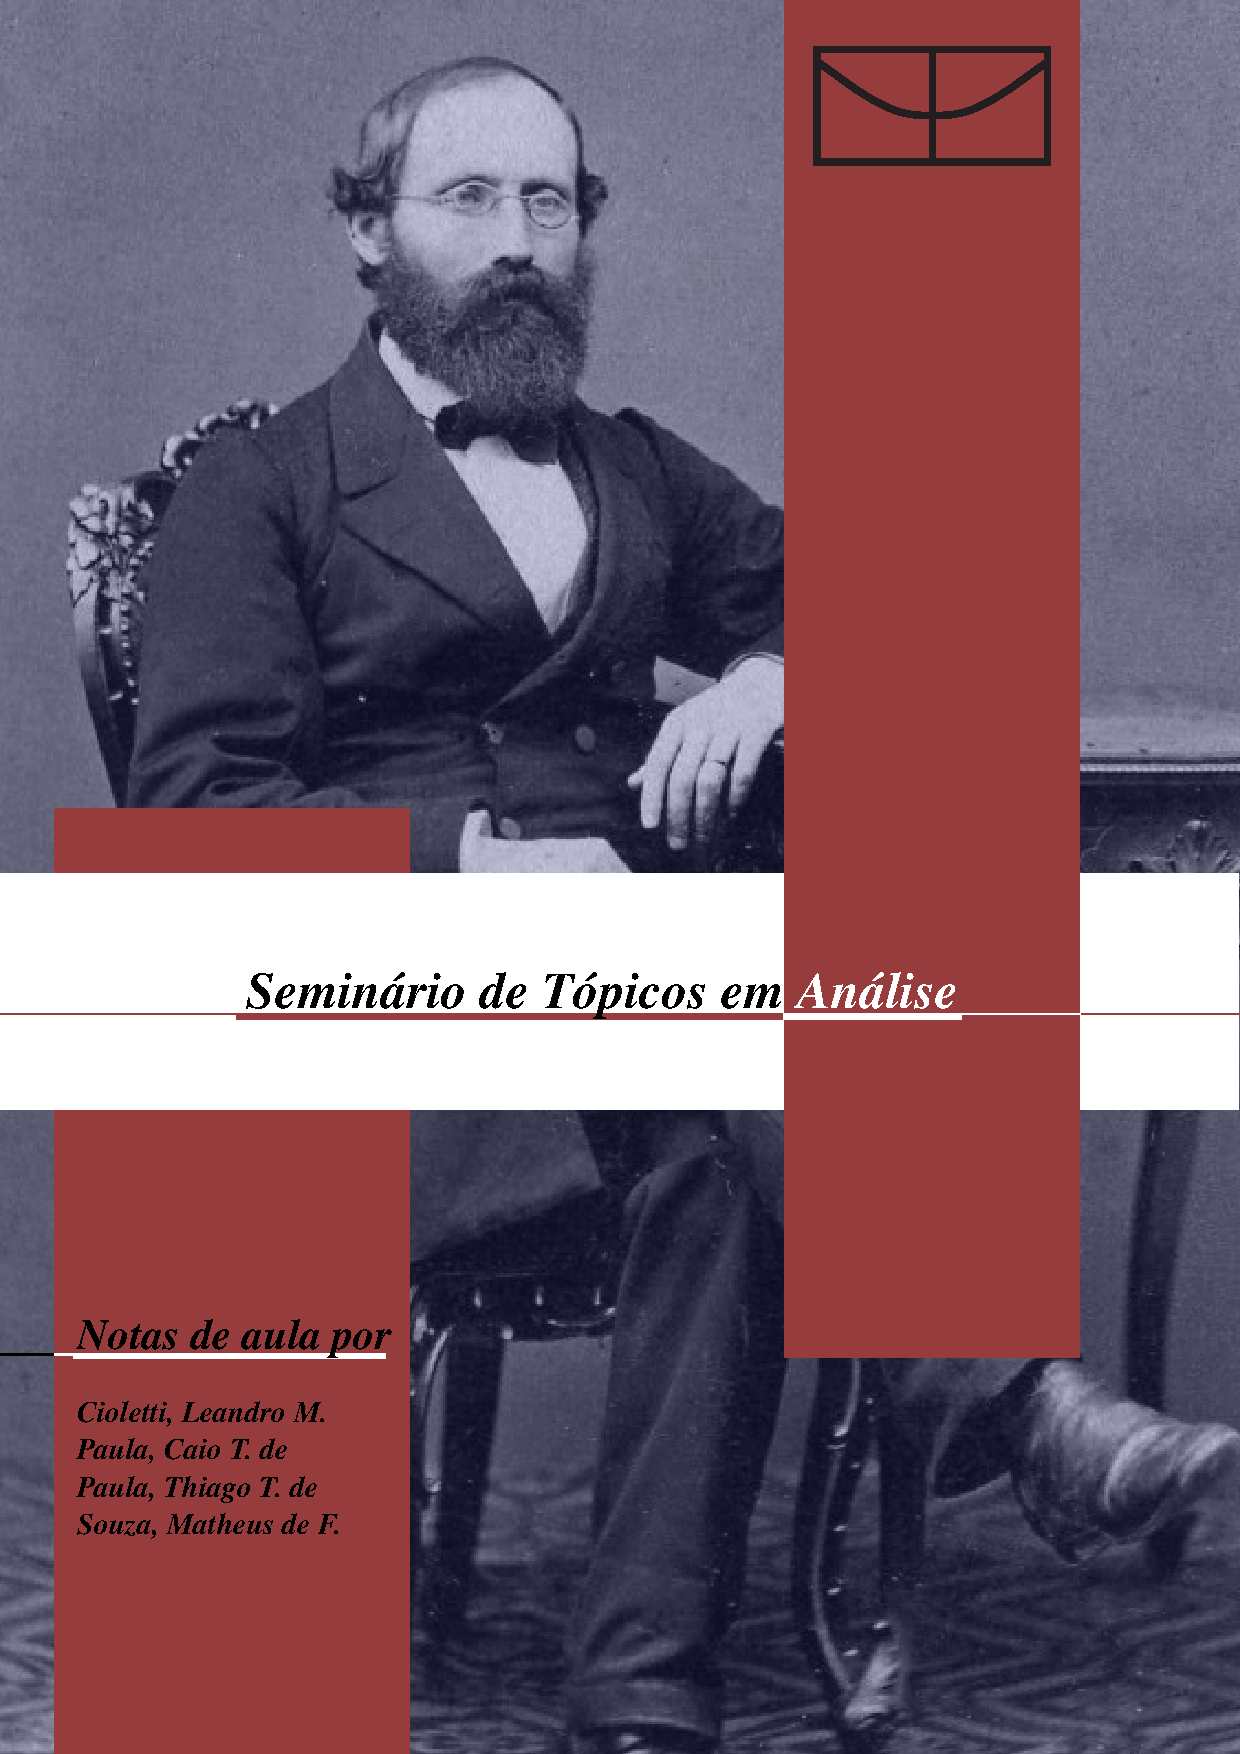
\includegraphics{Figuras/capa.pdf}
        };
    \end{tikzpicture}
\end{titlepage}

\loadgeometry{origin}% restore the origin margin setting

%%%%%%%%%%%%%%%%%%%%%%%

\noindent
{\huge Autores}
\\[0.3cm]
Leandro Cioletti, Caio Tomás, Matheus Freitas, Thiago Tomás
\\
\bigskip
\\[-0.1cm]
Versão 1.  Janeiro -- Maio de 2022
\\[0.3cm]
\noindent



\vfill
{\fontsize{14pt}{14pt}\selectfont
	\noindent
   \textbf{Seminário de Tópicos em Análise \\ Notas de Aula.  Janeiro -- Maio de 2022}
   \footnote{
   		Copyright \copyright\ 
   		\textbf{2022 Leandro Cioletti, Caio Tomás, Matheus Freitas, Thiago Tomás -- Todos os direitos reservados.}
   	}
 }



%%%%%%%%%%%%%%%%%%%%  Índice
\tableofcontents
\addtocontents{toc}{~\hfill\textbf{Página}\par}



% Cria o ambiente de Lista de Exercicios
% Não numerado e com a decoração igual ao
% das Aulas - Isto é na verdade apenas uma
% modificação do chapter*
%%\makeatletter
%%
%%\ChNameVar{\fontsize{14}{16}\usefont{OT1}{phv}{m}{n}\selectfont}
%%\ChNumVar{\fontsize{60}{62}\usefont{OT1}{ptm}{m}{n}\selectfont}
%%\ChTitleVar{\Huge\bfseries\rm}
%%\ChRuleWidth{1pt}
%%
%%
%%\renewcommand{\DOTIS}[1]{%
%%
%%\settowidth{\px}{\CNV\FmN{Lista de Exerc\'icios}}
%%    \addtolength{\px}{2pt}
%%    \settoheight{\py}{\CNV\FmN{Lista de Exerc\'icios}}
%%    \addtolength{\py}{1pt}
%%
%%    \settoheight{\pyy}{\CNoV\thechapter}
%%    \addtolength{\pyy}{-2pt}
%%    \setlength{\myhi}{\pyy}
%%    \addtolength{\myhi}{-1\py}
%%    \par
%%    \parbox[b]{\textwidth}{%
%%    \rule[\py]{\RW}{\myhi}%
%%    \hskip -\RW%
%%    \rule[\pyy]{\px}{\RW}%
%%    \hskip -\px%
%%    \raggedright%
%%    \CNV\FmN{Lista de Exerc\'icios}\space\CNoV %
%%    \hskip1pt%
%%    \mghrulefill{\RW}%
%%    \rule{\RW}{\pyy}\par\nobreak%
%%    \vskip -\baselineskip%
%%    \vskip -\pyy%
%%    \hskip \mylen%
%%    \mghrulefill{\RW}\par\nobreak%
%%    \vskip \pyy}%
%%    \vskip -2\p@}
%%\makeatother
%%%
 
%%%%%%%%%%%%%%%%%%%% Conteúdo das aulas    
\mainmatter 

\addcontentsline{toc}{part}{%
    \fontfamily{ptm}\selectfont\textit{Preliminares}
}
\part*{%
    \fontfamily{ptm}\selectfont\textit{Preliminares}
}

%\chapter{Background necessário}

% def integral complexa
% teo resíduos
% séries de potência (talvez resumir)
% princípio da identidade
% conceitos de topologia

\section{Introdução}
% apresentar o que é o texto, em que contexto foi feito...

\section{Conceito de Topologia}


\section{A integral complexa}


\section{O Teorema dos Resíduos}


\section{Séries de potência}


\section{Princípio da Identidade}

% Semana 1 
%% !TeX spellcheck = pt_BR
\chapter[Semana 1]{}
\chaptermark{}


\hfill%
\begin{minipage}{10cm}
\begin{flushright}
\rightskip=0.5cm
\textit{``You know also that the beginning is the most important part of any work''}
\\[0.1cm]
\rightskip=0.5cm
---Plato's Republic
\end{flushright}
\end{minipage}


\section{Introdução}

O conjunto dos números complexos $\mathbb{C}$
pode ser construído de diversas maneiras.
Algumas destas construções adotam abordagens puramente algébricas,
enquanto outras são um pouco mais geométricas. O objetivo desta seção 
é apresentar três alternativas para se construir o conjunto dos números complexos. 

Sem dúvida, entre todas as construções conhecidas a mais simples (porém abstrata) é aquela que introduz 
o conjunto dos número complexos como um conjunto abstrato de símbolos munido de duas operações binárias (soma e produto). 
Seus elementos são simplesmente símbolos da forma $a+ib$, onde $a$ e $b$ podem ser quaisquer números reais 
e a letra ``$i$\,'' é simplesmente um símbolo especial que será chamado de 
unidade imaginária.\index{Unidade imaginária} 
Por exemplo, $1+i\pi$ é um elemento deste conjunto. Mas como nada foi dito ainda sobre as operações algébricas, 
por enquanto o símbolo $1+i\pi$ só tem o significado de ser um amontoado 
4 caracteres escritos numa ordem especial. Em particular, nesta notação, apesar de sugerir, 
o símbolo ``$+$'' ainda não tem significado de uma soma e nem o símbolo $i\pi$
de um produto. Poderíamos prosseguir com a brincadeira 
(sem graça e aparentemente sem sentido) de listar mais elementos deste conjunto, escrevendo por exemplo símbolos como
$7+i3$ ou $\frac{1}{2}+i9$ e assim por diante. 
Claramente, nada de interessante apareceria disto e muito menos claro ainda seria qual a 
relação deste conjunto com a ideia intuitiva de que já temos do que sejam números. 

As responsáveis por estabelecer a relação entre o conjunto dos símbolos da forma $a+ib$ e a ideia de números 
são as operações algébricas de soma e produto definidas abaixo:
\begin{itemize}
\item $(a+ib)+(c+id) = (a+c)+i(b+d)$
\item $(a+ib)\cdot (c+id) = (ac-bd)+i(ad+bc)$.
\end{itemize}

Vamos ver agora um pouco do porquê a introdução destas operações dá vida 
à notação que usamos
para apresentar o conjunto $\mathbb{C}$. 
Primeiro observe que se identificamos um elemento da forma $a+i0$ 
com o número real $a$, então podemos pensar que as operações 
definidas acima são extensões das operações usuais de soma e produto de números reais. 
Isto é, a soma dos números complexos identificados com os números reais $a$ e $c$ é dada por 
$(a+i0)+(c+i0)=(a+c)+i0$ e portanto identificada com o número real $a+c$. Analogamente, 
o produto dos números complexos identificados com os números reais $a$ e $c$, é dado pela expressão
$(a+i0)\cdot(c+i0)=ac+i0$ que por sua vez é identificada com o número real $ac$. 

Da forma como foram definidas as operações em $\mathbb{C}$
somos levados naturalmente a identificar a unidade imaginária $i$ com o 
número complexo $0+i1$. Consequentemente, temos a relação
$i^2 = i\cdot i = (0+i1)\cdot(0+i1)= -1+0i = -1$. 
Desta simples observação podemos concluir que existe pelo menos 
um número complexo $z=a+ib\in \mathbb{C}$ 
que resolve a equação $z^2+1=0$. Este fato enfatiza a importância 
da unidade imaginária dentro do conjunto $\mathbb{C}$, já que não existe nenhum número 
real $x$ tal que $x^2+1=0$. Seguindo, vemos que a definição de produto nos permite interpretar 
o símbolo $ib$ em $a+ib$ como um produto da unidade imaginária pelo número real $b$. 
Para isto usamos primeiros as identificações mencionadas acima, em seguida que  
$i\cdot b = (0+i1)(b+0i)=0+ib$ e por último identificamos $0+ib$ com $ib$ obtendo 
a interpretação desejada. 
O leitor mais atento deve ter observado que até este momento fomos cuidadosos com a ordem dos termos da
nossa notação. Vamos voltar a este assunto mais a frente. 

%Mas a verdade é que usando as identificações já mencionadas e as operações 
%definidas acima, podemos verificar, por exemplo, que $i\cdot d$ e $d\cdot i$ representam o mesmo 
%número complexo. De fato, $i\cdot d = (0+i1)(d+i0) = 0+id = (d+i0)(0+id) = d\cdot i$.
%Mais geralmente, dados quaisquer números complexos $a+ib$ e $c+id$ temos que  
%Consequentemente, podemos olhar para 

Com o exposto até aqui já podemos imaginar como proceder para extrair
as demais propriedades algébricas básicas dos números complexos.
Por outro lado, uma boa parcela dos leitores deve ter ficado com a sensação de que esta é uma 
construção muito abstrata e um tanto quanto artificial. Para remediar isto, vamos
apresentar, em seguida, outra construção de caráter também algébrico, porém feita a partir de objetos matemáticos
bem mais familiares, matrizes! 

\bigskip 


Antes de prosseguir observamos que independentemente de como seja construído o conjunto dos números 
complexos nele sempre devem existir três elementos muito especiais: 
\begin{itemize}
	\item uma unidade imaginária, tradicionalmente denotada por $i$;
	\item um elemento neutro para a operação de produto, frequentemente denotado por $1$ ou $\mathds{1}$; 
	\item um elemento neutro para a operação de soma, frequentemente denotado pelo símbolo $0$.
\end{itemize}
Além do mais, é fundamental, em qualquer que seja a construção, que a seguinte
propriedade seja válida:
\\[0.3cm]
(P1) - o quadrado da unidade imaginária (quadrado com relação ao produto definido) somado ao elemento neutro do produto
de ser igual ao elemento neutro da soma. 
\\[0.3cm]

A fim de apresentar uma nova construção do conjunto dos números complexos 
satisfazendo a propriedade (P1) vamos explorar o espaço de matrizes. A exposição feita aqui é semelhante
à apresentada na referência \cite{MSoa16}. 
A princípio esta estratégia poderia soar um pouco estranha, mas a verdade é que o conjunto 
de matrizes com suas operações usuais é uma das poucas estruturas algébricas fora da lista
$\mathbb{N}$, $\mathbb{Z}$, $\mathbb{Q}$ e $\mathbb{R}$ que conhecemos quando estamos começando a estudar
matemática.

Como já mencionamos, certos espaços de matrizes já possuem estruturas naturais 
de soma e produto e assim parte das tarefas
da construção (que consiste em apresentar as propriedades algébricas) já estariam realizadas.
Por questão de simplicidade, é mais prudente iniciar nossa exploração pelo mundo das matrizes $2\times 2$ com entradas reais.
É claro que mais simples ainda seria começar pelas matrizes $1\times 1$ com entradas reais, 
porém este espaço com suas operações usuais é idêntico (do ponto de vista algébrico) ao 
conjunto dos números reais. Desta forma não seria possível 
escolher nenhum elemento dentro deste conjunto para fazer o papel da unidade imaginária de 
forma que a propriedade (P1), nele, fosse satisfeita.

Denote por $\mathbb{M}_{2\times 2}(\mathbb{R})$ o conjunto de todas as matrizes $2\times 2$ com entradas reais.
Vamos adotar as notações $\mathds{1}$ e $0$ para denotar, respectivamente, as matrizes: identidade e nula em $\mathbb{M}_{2\times 2}(\mathbb{R})$. Isto é, 
\[
\mathds{1}
\equiv
\begin{pmatrix}
1&0\\
0&1
\end{pmatrix} 
\qquad\text{e}\qquad 
0 
\equiv
\begin{pmatrix}
0&0\\
0&0
\end{pmatrix}.  
\]
Lembre-se que $\mathds{1}$ é o elemento neutro da operação usual de produto em $\mathbb{M}_{2\times 2}(\mathbb{R})$
e $0$ é o elemento neutro da soma, neste conjunto. 
Portanto, perguntar se a propriedade (P1) é satisfeita
em $\mathbb{M}_{2\times 2}(\mathbb{R})$ é equivalente a perguntar se existe
alguma matriz $X\in \mathbb{M}_{2\times 2}(\mathbb{R})$ satisfazendo 
\[
X\cdot X +\mathds{1} =0
\qquad \text{equivalentemente} \qquad 
X^2+\mathds{1}= 0.
\]
Se tal matriz existir ela é candidata natural para representar a unidade imaginária. 

Para resolver a equação acima, precisamos verificar se existem $x,y,z,w\in\mathbb{R}$ tais que 
\[
\begin{pmatrix}
x&y\\
z&w
\end{pmatrix}
\cdot
\begin{pmatrix}
x&y\\
z&w
\end{pmatrix}
+
\begin{pmatrix}
1&0\\
0&1
\end{pmatrix}
=
\begin{pmatrix}
0&0\\
0&0
\end{pmatrix}.
\] 
Com um pouco de paciência e utilizando o velho método de tentativa e erro, descobrimos rapidamente que 
o problema acima admite a solução $x=0$, $y=-1$, $z=1$ e $w=0$. Desta forma temos um candidato a unidade 
imaginária, que respeitando a tradição será denotado por
\[
i
=
\begin{pmatrix}
0&-1\\
1&0
\end{pmatrix}.
\]

Apesar da propriedade (P1) ser satisfeita em $\mathbb{M}_{2\times 2}(\mathbb{R})$, não podemos
usar o espaço como um todo para construir o conjunto $\mathbb{C}$. Uma das razões, que não mencionamos anteriormente, 
é que independentemente de como construímos $\mathbb{C}$ a operação de produto deve ser comutativa.
Por outro lado, é bem conhecido que a operação de produto em $\mathbb{M}_{2\times 2}(\mathbb{R})$ não é comutativa. 
Apesar desta nossa tentativa inicial ter sido frustrada rapidamente por esta obstrução, 
restaria ainda a esperança de se prosseguir
com a construção considerando um subconjunto próprio de $\mathbb{M}_{2\times 2}(\mathbb{R})$ 
em que a operação de produto fosse comutativa. 
Adotando esta estratégia a primeira coisa que viria em mente é restringir nossa atenção apenas ao subconjunto 
das matrizes diagonais em $\mathbb{M}_{2\times 2}(\mathbb{R})$, pois sabemos que a multiplicação de matrizes restritas 
a este subconjunto é certamente comutativa. 
Mas, infelizmente, isto nos causaria outro problema. A candidata à unidade imaginária, 
construída acima, não é um elemento do conjunto das matrizes diagonais. 
Já que a candidata a unidade imaginária proposta acima foi construída pelo método de erro e tentativa,  
poderíamos voltar à equação $X^2+\mathds{1}=0$ e verificar 
se seria possível encontrar uma matriz diagonal em $\mathbb{M}_{2\times 2}(\mathbb{R})$ 
que resolvesse este problema. Após alguns poucos cálculos descobriríamos que nenhuma matriz 
diagonal em $\mathbb{M}_{2\times 2}(\mathbb{R})$ pode ser uma solução desta equação.


Para continuar nossa busca precisamos investigar se existem outros 
subconjuntos de $\mathbb{M}_{2\times 2}(\mathbb{R})$ que além de possuir a nossa já construída unidade imaginária 
seja tal que a operação de produto restrita a ele é comutativa. 
Isto nos leva naturalmente a considerar a seguinte pergunta. 
\\
{\bf Pergunta.} Existe algum subconjunto de 
$\mathscr{C}\subset \mathbb{M}_{2\times 2}(\mathbb{R})$ possuindo a nossa candidata à unidade imaginária e também satisfazendo a seguinte propriedade: para quaisquer $A,B\in \mathscr{C}$ temos 
$A\cdot B = B\cdot A$? 

Uma maneira de atacar este problema é começar construindo uma coleção matrizes, a mais simples possível, 
de forma que todos os elementos deste conjunto comutem entre si e também com a matriz
\[
i= 
\begin{pmatrix}
0&-1\\
1&0
\end{pmatrix}.
\]

Para isto vamos usar o fato bem conhecido de que a matriz identidade $\mathds{1}$ comuta com qualquer
matriz e em particular com a matriz $i$. Na verdade, para todo $a\in\mathbb{R}$ 
temos que a matriz 
\[
a\mathds{1} 
= 
\begin{pmatrix}
a&0\\
0&a
\end{pmatrix}
\] 
comuta com a matriz $i$. De forma mais geral, dados quaisquer $a,b\in\mathbb{R}$
temos que as matrizes
\[
a\mathds{1} 
= 
\begin{pmatrix}
a&0\\
0&a
\end{pmatrix}
\qquad \text{e}\qquad 
bi= 
\begin{pmatrix}
0&-b\\
b&0
\end{pmatrix}
\]
comutam. 

Antes de prosseguir aproveitamos para observar que este é um bom momento 
para falarmos sobre a operação de soma, que permaneceu por um tempo 
esquecida da nossa discussão. O que queremos dizer é que em qualquer construção de $\mathbb{C}$
a soma de quaisquer dois elementos deste conjunto deve também ser um elemento deste conjunto. 
Desta forma nossa construção dos números complexos precisa possuir o elemento 
\[
a\mathds{1}+b i = 
\begin{pmatrix}
a&0\\
0&a
\end{pmatrix}
+
\begin{pmatrix}
0&-b\\
b&0
\end{pmatrix}
=
\begin{pmatrix}
a&-b\\
b&a
\end{pmatrix}.
\]
Isto nos motiva a propor o seguinte conjunto de $\mathbb{M}_{2\times 2}(\mathbb{R})$ 
como uma construção do conjunto dos números complexos
\[
\mathbb{C}
= 
\left\{
\begin{pmatrix}
a&-b\\
b&a
\end{pmatrix}
:
a,b\in \mathbb{R}
\right\}.
\] 

Várias propriedades exigidas de uma construção do conjunto dos números complexos já 
foram verificadas para este conjunto. Seguindo nossas notações uma matriz arbitrária 
pertencente ao nosso conjunto $\mathbb{C}$ pode ser escrita 
como $a\mathds{1}+ bi$ onde $a,b\in\mathbb{R}$.

Uma outra propriedade importante que ainda não mencionamos sobre a construção de $\mathbb{C}$
é que todo elemento não-nulo deve possuir um inverso multiplicativo. 
Isto é, para todo $a\mathds{1}+ bi$ em $\mathbb{C}$ deve existir um elemento $c\mathds{1}+ di$ em $\mathbb{C}$
tal que $(a\mathds{1}+ bi)\cdot (c\mathds{1}+ di) = \mathds{1}$. 
O inverso multiplicativo de $a\mathds{1}+ bi$ é normalmente denotado por $(a\mathds{1}+ bi)^{-1}$.

Apesar da nossa construção
não ter levado isto em conta, esta propriedade será válida. Para verificar este fato, vamos começar 
recordando que uma matriz $A\in \mathbb{M}_{2\times 2}(\mathbb{R})$  possui uma inversa se, e somente se,
$\mbox{det}(A)\neq 0$. No nosso caso temos
\[
\mbox{det}(a\mathds{1}+ bi) 
= 
\mbox{det}
\begin{pmatrix}
a&-b\\
b&a
\end{pmatrix}
=
a^2+b^2.
\]
Portanto, se $a$ ou $b$ for não-nulo então existe a inversa de $a\mathds{1}+ bi$. 
Como estamos trabalhando com matrizes $2\times 2$, conhecemos explicitamente a forma de sua inversa.
Mais precisamente, nos casos em que $a$ ou $b$ são não-nulos o inverso multiplicativo de $a\mathds{1}+ib$
sempre existe e é dado por
\[
(a\mathds{1}+ bi)^{-1} 
= 
\begin{pmatrix}
a&-b\\
b&a
\end{pmatrix}^{-1}
=
\frac{1}{a^2+b^2}
\begin{pmatrix}
a&b\\
-b&a
\end{pmatrix}
=
\frac{a}{a^2+b^2}\mathds{1}
+
\frac{-b}{a^2+b^2}i,
\]
o que permite verificar imediatamente que a matrix $(a\mathds{1}+ bi)^{-1}$ 
está no nosso conjunto $\mathbb{C}$. 

Resta ainda mostrar que o produto entre duas matrizes do conjunto definido acima 
resulta em outra matriz que também pertence a este conjunto e que 
elas comutam entre si. 
De fato, dados dois elementos arbitrários $(a\mathds{1}+ bi)$ e $(c\mathds{1}+ di)$ 
do nosso conjunto $\mathbb{C}$, temos que
\begin{align*}
(a\mathds{1}+ bi)\cdot(c\mathds{1}+ di)
&=
\begin{pmatrix}
a&-b\\
b&a
\end{pmatrix}
\begin{pmatrix}
c&-d\\
d&c
\end{pmatrix}
\\
&=\begin{pmatrix}
ac-bd& -(ad+bc)\\
(ad+bc)&ac-bd
\end{pmatrix}
\\
&=
(ac-bd)\mathds{1}+ (ad+bc)i.
\end{align*}
Procedendo das mesma maneira podemos verificar que 
\begin{align*}
(a\mathds{1}+ bi)\cdot(c\mathds{1}+ di)
&=
\begin{pmatrix}
a&-b\\
b&a
\end{pmatrix}
\begin{pmatrix}
c&-d\\
d&c
\end{pmatrix}
\\
&=
\begin{pmatrix}
c&-d\\
d&c
\end{pmatrix}
\begin{pmatrix}
a&-b\\
b&a
\end{pmatrix}
=
(c\mathds{1}+ di)\cdot(a\mathds{1}+ bi).
\end{align*}

Este argumento conclui a nossa construção do conjunto do números complexos. 
Antes de passar para a próxima construção que terá um caráter mais geométrico
observamos que se, por um abuso de notação, omitimos o símbolo $\mathds{1}$ 
da notação $a\mathds{1}+ib$, então ficamos com simplesmente com $a+ib$. 
Este pequeno abuso de notação tornaria a notação dos elementos desta nova 
construção praticamente indistinguível 
daquela usada na construção apresentada no inicio deste capítulo. 


\section{O Corpo dos Números Complexos}

%%%%%%%%%%% Fancy Quote 
\vspace{0.5cm}
\hfill%
\begin{minipage}{10cm}
\begin{flushright}
\rightskip=0.5cm
\textit{``The sweeping development of mathematics during the last two centuries is
due in large part to the introduction of complex numbers; paradoxically, this is based
on the seemingly absurd notion that there are numbers whose squares are negative''}
\\[0.1cm]
\rightskip=0.5cm
---E. Borel, 1952
\end{flushright}
\end{minipage}
\vspace{1cm}


Nesta seção vamos apresentar a prometida construção geométrica dos números complexos $\mathbb{C}$
e em seguida vamos apresentar a definição do que é uma estrutura algébrica chamada de corpo.

O caráter geométrico presente nesta nossa próxima construção vem do 
fato que de agora vamos pensar o conjunto $\mathbb{C}$ como sendo o conjunto de todos
os pontos do espaço Euclideano bi-dimensional $\mathbb{R}^2 = \{(x,y) : x,y\in \mathbb{R}\}$.
Desta forma um ponto $z\in\mathbb{C}$ é representado por $z=(x,y)$ e portanto podemos
pensar que os pontos de $\mathbb{C}$ são vetores. 
Agora precisamos definir as operações de soma e produto entre estes elementos. 
A soma é definida como sendo a soma usual de vetores, isto é, se $z=(a,b)$ e $w=(c,d)$
então $z+w=(a+c,b+d)$. A multiplicação, por sua vez, é definida da seguinte maneira 
$z\cdot w = (ac-bd,ad+bc)$. 

Desta forma o elemento neutro da operação de soma é dado pelo vetor 
$(0,0)$ que denotaremos simplesmente por $0$. 
Já o  neutro da multiplicação será o vetor $(1,0)$, que denotaremos por $\mathds{1}$. 
Por último verificamos que a unidade imaginária é representada pelo vetor $(0,1)$,
que também será denotado simplesmente por $i$. Desta forma um número complexo $z=(a,b)$ pode ser 
escrito como $a\mathds{1}+ib$, onde $ib$ representa simplesmente a multiplicação do escalar $b$
pelo vetor $(0,1)$. Podemos novamente abusar da notação e omitir como na construção anterior o 
símbolo $\mathds{1}$ e assim escrever um número complexo simplesmente na forma $a+ib$.

Antes de continuar é importante entender a diferença do significado da notação $a+ib$ nos 
três contextos discutidos até agora: 

\begin{itemize}
\item na primeira construção $a+ib$ significava apenas uma concatenação de 4 caracteres;

\item na segunda construção $a+ib$ representava a matriz 
$\begin{pmatrix}
a&-b\\
b&a
\end{pmatrix}
\in
\mathbb{M}_{2\times 2}(\mathbb{R})
$;

\item nesta terceira construção $a+ib$ representa o vetor $(a,b)\in \mathbb{R}^2$.
\end{itemize}

Afinal de contas o que há de comum nesta três construções? Existem então três conjuntos distintos 
de números complexos? Ou melhor o que é ``o'' conjunto dos números complexos?


A resposta para a primeira pergunta está ligada ao conceito de \textit{corpo}. 


\begin{definicao}[Corpo] 
\index{Corpo}
Um conjunto não-vazio $\mathscr{C}$ munido de duas operações 
binárias, digamos ``$+$'' e ``$\cdot$'' é chamado de corpo se as seguintes propriedades são satisfeitas.
Dados $z,z_1,z_2,z_3\in \mathscr{C}$ temos:
\begin{enumerate}[\bf (1)] 
\item comutatividade: $z_1+z_2=z_2+z_1$ \quad e \quad $z_1\cdot z_2 = z_2\cdot z_1$;

\item associatividade: $(z_1+z_2)+z_3 = z_1+(z_2+z_3)$ 
\quad e \quad $z_1\cdot(z_2\cdot z_3)=(z_1\cdot z_2)\cdot z_3$;

\item distributividade: $z_1\cdot (z_2+z_3)=z_1\cdot z_2+ z_1\cdot z_3$;

\item elemento neutro para operação ``$+$'': isto é, existe um elemento em $\mathscr{C}$ denotado por $0$
satisfazendo $0+z=z$;

\item elemento neutro para operação ``$\cdot$'': isto é, existe um elemento em $\mathscr{C}$ denotado por $1$
satisfazendo $1\cdot z=z$;

\item todo elemento $z\in \mathscr{C}$ possui um simétrico para operação ``$+$'', denotado por $(-z)$, tal que 
$z+(-z)=0$;

\item  todo elemento $z\in \mathscr{C}$ diferente do elemento $0$ possui um inverso para operação ``$\cdot$'', ou seja
existe um elemento denotado por $z^{-1}$ tal que $z\cdot z^{-1}=1$. 
\end{enumerate}
\end{definicao}

A operação ``$+$'' que aparece na definição acima é em muitos contextos chamada de soma e a operação
``$\cdot$'' é chamada de produto. A última, por sua vez, é até frequentemente omitida. 
Um corpo é então um conjunto $\mathscr{C}$ munido de duas operações binárias ``$+$'' e ``$\cdot$''
de forma que as condições de (1) a (7) da definição acima são satisfeitas.
Desta maneira um corpo deve ser entendido como o trio ordenado $(\mathscr{C},+,\cdot)$. 
Quando não houver perigo de confusão com relação a quem são as operações binárias,
vamos denotá-lo simplesmente por $\mathscr{C}$.

\bigskip 

Seguimos agora com resposta para a segunda pergunta. 
A rigor a resposta é afirmativa já que os conjuntos em cada uma das três construções
apresentadas são completamente distintos. Por outro lado, estas três estruturas algébricas
têm algo em comum que fazem com que do ponto de vista algébrica elas sejam indistinguíveis 
entre si. Isto é expresso de maneira precisa pela ideia 
de \textit{isomorfismo} de corpos. 


\begin{definicao}[Isomorfismos de Corpos]\label{def-isomorfismo-corpos}
\index{Isomorfismo}
Dizemos os dois corpos $(\mathscr{C},+,\cdot)$ e $(\mathscr{D},\oplus,\odot)$ são 
isomorfos se existe uma bijeção $\varphi:\mathscr{C}\to\mathscr{D}$ tal que $\varphi$ 
e sua inversa $\varphi^{-1}$ preservam 
as operações binárias. Isto é, para todos $x,y\in\mathscr{C}$ e $u,v \in\mathscr{D}$
temos que:
\begin{itemize} 
\item 
$\varphi(x+y)=\varphi(x)\oplus\varphi(y)$ \quad e \quad $\varphi(x\cdot y)=\varphi(x)\odot \varphi(y)$;
\item 
$\varphi^{-1}(u\oplus v)=\varphi^{-1}(u)+\varphi^{-1}(v)$ \quad e \quad
$\varphi^{-1}(u\odot v)= \varphi^{-1}(u)\cdot \varphi^{-1}(v)$.
\end{itemize}
\end{definicao} 


É possível mostrar que as três construções apresentadas nestas notas definem três corpos distintos e
além do mais que estes três corpos são dois-a-dois isomorfos, no sentido da definição dada acima.


Agora estamos prontos para responder a última pergunta. O que é o conjunto dos números complexos?
Neste texto o conjunto dos números complexos $\mathbb{C}$
será definido como o conjunto apresentado na primeira
construção. É claro pelos comentários anteriores que não há diferença de pensar nos pontos 
de $\mathbb{C}$ como vetores de $\mathbb{R}^2$ ou mesmo como matrizes $2\times 2$. Estes pontos
de vista vão ajudar a compreender melhor os problemas a serem estudados. 
Para exemplificar isto, observamos que é mais fácil entender o significado da operação da soma $z+w$
pensando nos pontos $z$ e $w$ sendo vetores. É mais fácil lembrar como funciona o produto
$z\cdot w$ pensando na representação matricial da segunda construção. E por último é mais
fácil fazer manipulações algébricas usando a primeira construção. 
Muito provavelmente em pouco tempo o leitor deve notar que estará 
trabalhando com as três construções/representações 
simultaneamente, sem perceber!


No restante desta seção faremos alguns cálculos simples para nos familiarizarmos com as operações
com números complexos. Começamos observando que para efetuar o produto de $z=x_1+iy_1$ 
e $w=x_2+iy_2$ basta usar as propriedades distributiva e comutativa juntamente 
com a identidade $i^2=-1$ como segue:
\begin{align*}
z\cdot w
=
(x_1+iy_1)\cdot(x_2+iy_2) 
&= 
x_1x_2+x_1iy_2+iy_1x_2+iy_1iy_2
\\
&=
x_1x_2+ix_1y_2+ix_2y_1+i^2y_1y_2
\\
&=
x_1x_2+i(x_1y_2+x_2y_1)-y_1y_2
\\
&=
x_1x_2-y_1y_2+i(x_1y_2+x_2y_1).
\end{align*}
Em particular, temos 
\begin{align}\label{eq-zvesesconjz}
(x+iy)(x-iy) = x^2+y^2.
\end{align}
Esta igualdade é bastante útil para ajudar a expressar quocientes de números complexos.
O seguinte exemplo ilustra este fato. Para reduzir
\[
\frac{(5+i\pi)+(-1+4i)}{\sqrt{3}+4i}
\]
à forma $x+iy$, primeiro simplificamos o numerador:
\[
\frac{(5+i\pi)+(-1+4i)}{\sqrt{3}+4i}
=
\frac{4+i(\pi+4)}{\sqrt{3}+4i}.
\]
Próximo passo consiste em observar que a expressão acima permanece inalterada 
se a multiplicamos e dividimos pelo número complexo $\sqrt{3}-4i$ 
\begin{align*}
\frac{4+i(\pi+4)}{\sqrt{3}+4i}
&=
\frac{4+i(\pi+4)}{\sqrt{3}+4i}\cdot 
\frac{\sqrt{3}-4i}{\sqrt{3}-4i}
\\
&=
\frac{(4+i(\pi+4)) (\sqrt{3}-4i)}{3^2+4^2}
\\
&=
\frac{(4\sqrt{3}+4\pi+16)+i(\sqrt{3}\pi+4\sqrt{3}-16)}{25}
\\
&=
\frac{(4\sqrt{3}+4\pi+16)}{25}+i\frac{(\sqrt{3}\pi+4\sqrt{3}-16)}{25}.
\end{align*}

Observe que uma identidade análoga a \eqref{eq-zvesesconjz} pode ser 
obtida considerando o caso mais geral em que os números reais $x$ e $y$ são substituídos por números complexos 
arbitrários $z$ e $w$, isto é, 
\[
(z+iw)\cdot(z-iw) = z^2-izw+w^2+iwz = z^2+w^2.
\]
Entretanto, neste caso mais geral, não é possível assegurar que 
o lado direito da igualdade acima seja um número positivo. Aliás é muito simples
construir diversos exemplos que este resultado é inclusive um número negativo!
Sugerimos que o leitor pense neste instante em um exemplo, 
para não cair na armadilha de pensar em $z^2$ como um número positivo.  

Vamos encerrar esta seção chamando atenção para duas propriedades importantíssimas 
ligadas a estrutura algébrica de corpo que o conjunto dos números complexos possui.

Um fato bem conhecido sobre os números reais é que se $x,y\in\mathbb{R}$ são tais 
que $x\cdot y=0$ então $x=0$ ou $y=0$. No conjunto dos números complexos esta 
propriedade permanece válida. Já que a operação de produto em $\mathbb{C}$ é bastante peculiar
esta generalização requer então uma prova. 

\begin{proposicao}
Sejam $z=a+ib$ e $w=c+id$ números complexos. 
Se $z\cdot w= 0$ então $z=0$ ou $w=0$.
\end{proposicao} 

\begin{proof}
Primeiro observamos que o produto de qualquer número complexo por zero é sempre zero.
Portanto se multiplicamos ambos os lados da igualdade $z\cdot w = 0$ pelo número complexo $(a-ib)(c-id)$
ficamos com 
\begin{align*}
z\cdot w\cdot (a-ib)(c-id) = 0\cdot (a-ib)(c-id) =0.
\end{align*}
Lembrando da identidade $(x+iy)(x-iy) = x^2+y^2$ podemos verificar que o lado esquerdo da igualdade acima
é dado por 
\begin{align*}
z\cdot w\cdot (a-ib)(c-id)
&=
(a+ib)(c+id) (a-ib)(c+id)
\\
&=
(a+ib)(a-ib)(c+id)(c+id)
\\
&=
(a^2+b^2)(c^2+d^2).
\end{align*}
Substituindo esta expressão na igualdade anterior concluímos que  
$(a^2+b^2)(c^2+d^2)=0$. Mas agora temos um produto de dois números reais igual zero.
Portanto pelo menos um dos fatores deve ser zero. Se for o primeiro, então $a^2+b^2=0$
mas então $a=0$ e $b=0$ logo $z=a+ib=0$. No outro caso o argumento é análogo.
\end{proof}


A afirmação da proposição acima é na verdade válida para um corpo qualquer. 
Explorando a estrutura de corpo somos conduzidos inclusive a apresentar uma prova
bem mais simples deste fato, usando uma ideia semelhante àquela empregada na prova 
acima. Basta observar que se $\mathscr{C}$ é um corpo e $u,v\in\mathscr{C}$ são tais 
que $u\cdot v =0$, então ou temos $u=v=0$ ou um deles é diferente de zero. Digamos $u\neq 0$.
Como estamos em um corpo e $u\neq 0$ então exite o inverso multiplicativo de $u$, isto é $u^{-1}$.
Multiplicando ambos lados da equação $u\cdot v =0$ por $u^{-1}$ ficamos com 
$u^{-1}\cdot u\cdot v = 0\cdot u^{-1}$. Simplificando as expressões em ambos os lados
concluímos que $v=0$. No caso $v\neq 0$ podemos usar argumentação semelhante já que a operação 
de produto é comutativa, o que permitiria trocar a ordem dos produtos e chegar à conclusão que $u=0$. 
Este é exemplo muito interessante em que considerar a estrutura abstrata inspira a escrita
de provas mais simples. 

A outra propriedade que queremos destacar é que diferentemente do conjunto dos números
reais o conjunto dos números complexos não admite uma relação de ordem compatível 
com a relação de ordem da reta. Vamos elaborar um pouco sobre isto. Em $\mathbb{R}$ 
sabemos que dados dois números distintos $x$ e $y$ uma das seguintes alternativas sempre é válida.
Ou $x<y$ ou $y<x$. Deste fato segue que o quadrado de qualquer número real não-nulo é sempre positivo.
Desta observação podemos concluir que não existe nenhuma relação de ordem 
em $\mathbb{C}$ compatível com a relação de ordem da reta já que $i^2=-1$. 


\section{Módulo, Conjugado, Partes Real e Imaginária}

Seja $z\in \mathbb{C}$ da forma $z=x+iy$, onde $x$ e $y$ são reais. 
Chamamos $x$ de parte real de $z$ e $y$ de parte imaginária de $z$ e nos referimos a elas 
usando as seguintes notações $x=\text{Re}(z)$ e $y=\text{Im}(z)$.
\index{Parte real}\index{Parte imaginária}
Pensando no número complexo $z$ como um ponto de $\mathbb{R}^2$, 
os números reais $\text{Re}(z)$ e $\text{Im}(z)$ representam as coordenadas de $z$.
O subconjunto de todos os pontos de $\mathbb{C}$ que satisfazem $\text{Im}(z)=0$ é
chamado às vezes de eixo real e pensando em $\mathbb{C}$ como $\mathbb{R}^2$
este conjunto então seria correspondente ao eixo $x$. Definimos também o eixo imaginário
como sendo o conjunto dos números complexos satisfazendo $\text{Re}(z)=0$. 

A noção de distância em $\mathbb{C}$ será definida de maneira semelhante a $\mathbb{R}^2$.
Primeiro definimos o módulo
\index{Módulo de $z$} de um número complexo $z=x+iy$ como sendo $|z|=\sqrt{x^2+y^2}$.
Note que o módulo de $z$ é exatamente a norma Euclideana do vetor de coordenadas $(x,y)$.
Em seguida, dados $z,w\in\mathbb{C}$ definimos a distância entre eles como sendo $|z-w|$.
Da observação anterior, segue que se pensamos que $z$ e $w$ são pontos
de $\mathbb{R}^2$ então $|z-w|$ representa exatamente a distância Euclidiana entre este dois pontos. 
Feita esta observação podemos concluir imediatamente que vale a desigualdade triangular 
\index{Desigualdade!Triangular}
também é válida em $\mathbb{C}$, isto é, 
\[
|z+w|\leq |z|+|w|,\quad \forall z,w\in\mathbb{C}.
\]

De maneira geral, podemos dizer que conceito de módulo importa para o conjunto dos números complexos
toda a geometria Euclidiana. Sendo assim é natural imaginar que novas relações geométricas devam surgir
da estrutura de produto presente em $\mathbb{C}$. Para explorar estas possibilidades vamos 
introduzir mais um conceito fundamental sobre números complexos.

\begin{definicao}
\index{Conjugado}
O conjugado de um número complexo $z=x+iy$ é definido por
$\bar{z}=x-iy$. 
\end{definicao}
\begin{figure}[h]
\centering
\vspace*{-0.4cm}
\includegraphics[scale=0.55]{"./Figuras/fig-conjugado-enquadrado"}
\caption{Os números complexos $z$ e $w$ representados no plano Euclidiano com seus respectivos conjugados.}
\label{fig:conjugado}
\end{figure}

Como ilustrado na Figura \ref{fig:conjugado}, $\bar{z}$ 
pode ser interpretado geometricamente como sendo a reflexão de $z$ em torno
do eixo real. 


Além do mais, podemos por meio da conjugação estabelecer uma forte relação entre produto (álgebra)
e o norma (geometria) em $\mathbb{C}$ que é dada pela identidade
\begin{align}\label{eq-zXzbarra}
z \bar{z} = (x+iy)(x-iy)=x^2+y^2 = |z|^2.
\end{align}


Abaixo vamos explorar o poder desta conexão apresentando uma prova da importantíssima
desigualdade triangular usando majoritariamente a estrutura algébrica de $\mathbb{C}$.
Antes, será conveniente apresentar algumas outras identidades que seguem diretamente
das definições de conjugado e módulo e algumas de suas consequências. 

\medskip 

Para todo $z,w\in \mathbb{C}$ com $z=x+iy$ as seguintes identidades são válidas:
\label{page:eq-prop-basicas-conjugado}
\begin{enumerate}[({I}.1)]
\item $x=\mathrm{Re}(z) = \frac{1}{2}(z+\bar{z})$;
\item $y= \mathrm{Im}(z) = \frac{1}{2i}(z-\bar{z})$;
\item $z$ está no eixo real, se e somente se, $z=\bar{z}$;
\item $\overline{\,\overline{z}\,}=z$;
\item $\overline{z+w}= \overline{z}+\overline{w}$;
\item $\overline{z\cdot w}=\overline{z}\cdot \overline{w}$;
\item $|zw|=|z||w|$;
\item se $w\neq 0$ então $\displaystyle \left| \frac{z}{w}\right| = \frac{|z|}{|w|}$;
\item $|\overline{z}| = |z|$.
\end{enumerate}

Observamos que (I.7)-(I.9) são consequências de (I.6). 
A prova destas identidades podem ser feitas de diversas maneiras. Abaixo mostramos
um argumento simples que fornece, por exemplo, (I.7) sem a 
necessidade de se trabalhar explicitamente das coordenadas dos
números complexos $z$ e $w$. 

Para obter (I.7) a partir de (I.6) basta proceder da seguinte maneira. 
Primeiro usamos a identidade \eqref{eq-zXzbarra} para o número complexo $zw$ e logo em seguida a 
identidade (I.6) para obter
\[
|zw|^2 
= 
zw\overline{zw} 
= 
zw\overline{z}\,\overline{w}= z\overline{z}w\overline{w} = |z|^2|w|^2.
\]
Para finalizar basta tomar raíz-quadrada de ambos os lados da igualdade acima
e lembrar que se $x$ e $y$ são números reais não-negativos, então $\sqrt{xy}=\sqrt{x}\sqrt{y}$.


\begin{proposicao}\label{eq-quadrado-modulo}
Para todos $z,w\in\mathbb{C}$ temos:
\begin{enumerate}[i)]
 \item $|z+w|^2= |z|^2+2\mathrm{Re}(z\bar{w})+|w|^2$;
 \item $|z-w|^2= |z|^2-2\mathrm{Re}(z\bar{w})+|w|^2$;
 \item $|z+w|^2+|z-w|^2 = 2(|z|^2+|w|^2)$.
\end{enumerate}
\end{proposicao}
\begin{proof}
Primeiro vamos mostar que a igualdade enunciada no item \textit{i)} é verdadeira para todo
$z,w\in\mathbb{C}$.  

Note que segue da igualdade \eqref{eq-zXzbarra} que 
\begin{align*}
|z+w|^2
&=
(z+w)\overline{(z+w)}
=
(z+w)(\overline{z}+\overline{w})
\\
&=
z\overline{z}+z\overline{w}+w\overline{z}+w\overline{w}.
\end{align*}
Usando (I.6) e (I.4) temos que 
$
\overline{\,z\overline{w}\,} 
= 
\overline{z}\overline{\,\overline{w}\,} 
=
\overline{z}w
=
w\overline{z}
$.
O que mostra que a segunda e a terceira parcelas do lado direito da igualdade
acima são conjugados uma da outra e vice-versa. 
Aplicando a identidade (I.1) ao número complexo $z\overline{w}$ e em seguida usando a observação 
feita no início deste parágrafo podemos concluir que 
$2\Re(z\overline{w}) = z\bar{w}+ \overline{z\overline{w}} = z\bar{w}+w\overline{z}$. 
Usando esta igualdade na expressão que obtivemos acima para $|z+w|^2$ 
e lembrando que $z\overline{z}=|z|^2$ concluímos finalmente que 
\[
|z+w|^2
=
z\overline{z}+z\overline{w}+w\overline{z}+w\overline{w}
=
|z|^2+2\Re(z\overline{w})+|w|^2.
\]

A prova de \textit{ii)} é consequência imediata do item \textit{i)}. De fato, basta substituir $w$ por $-w$,
aplicar (I.6) depois (I.3) para verificar que 
\[
\Re\big(z\overline{(-w)}\big)
= 
\Re\big(z\overline{(-1)w}\big) 
=  
\Re\big(z\overline{(-1)}\overline{w}\big)
=
- \Re(z\overline{w})
\] 
e observar que $|w|=|-w|$. 

Para provar o item \textit{iii)} basta somar lado-a-lado os dois itens anteriores.
\end{proof}

\bigskip 

Precisamos estabelecer mais dois fatos antes de apresentarmos a nossa 
prometida prova puramente algébrica da desigualdade triangular.
Este fatos são na verdade estimativas das partes real e imaginária
de um número complexo. Apesar da prova destas estimativas serem bastante simples, elas serão muito úteis por todo o texto.

\begin{lema}\label{lema-re-im-modulo}
Para qualquer $z\in\mathbb{C}$ temos 
\begin{align*}
-|z|\leqslant \Re(z)\leqslant |z|\phantom{.}
\\[0.3cm]
-|z|\leqslant \Im(z)\leqslant |z|.
\end{align*}
\end{lema}
\begin{proof}
Esta prova é baseada em alguns fatos simples sobre números reais que serão recordados neste momento.
O primeiro deles é o seguinte: se $x$ e $y$ são quaisquer números reais satisfazendo $|x|\leq |y|$,
então $-|y|\leqslant x\leqslant |y|$. Outros fatos importantes que vamos utilizar são:
\begin{itemize}
\item a função raíz-quadrada é uma função monótona não-decrescente, isto é, 
para todo $0\leqslant x\leqslant y$ temos $\sqrt{x}\leqslant\sqrt{y}$; e 
\item $\sqrt{x^2}=|x|$. 
\end{itemize}

Já que para quaisquer $x,y\in\mathbb{R}$
temos sempre $x^2\leqslant x^2+y^2$ e também $y^2\leqslant x^2+y^2$ 
segue dos fatos citados acima que  
\[
|x| = \sqrt{x^2}\leqslant\sqrt{x^2+y^2}
\quad\text{e}\quad
|y| = \sqrt{y^2}\leqslant\sqrt{x^2+y^2}.
\]


Já que qualquer número complexo $z$ pode sempre ser escrito da seguinte forma $z=\Re(z)+i\Im(z)$,
temos da definição de módulo de um número complexo e das desigualdades acima para $x=\Re(z)$ e $y=\Im(z)$ que 
\[
|\Re(z)| \leqslant  \sqrt{(\Re(z))^2+(\Im(z))^2} = |z|
\]
e
\[
|\Im(z)| \leqslant  \sqrt{(\Re(z))^2+(\Im(z))^2} = |z|
\]
Destas duas desigualdades e da observação sobre números reais feita no primeiro parágrafo desta prova, temos que 
\begin{align*}
-|z|\leqslant \Re(z)\leqslant |z|\phantom{.}
\\[0.3cm]
-|z|\leqslant \Im(z)\leqslant |z|.
\end{align*}
\end{proof}

Após estes longos preparativos, agora temos tudo pronto para finalmente apresentar nossa prova 
algébrica para a desigualdade triangular.
\begin{teorema}[Desigualdade Triangular]
\label{teo-des-triang}
\index{Desigualdade!Triangular}
Para todo $z,w\in\mathbb{C}$ temos 
\[|z+w|\leqslant |z|+|w|.\]
\end{teorema}
\begin{proof}
Sejam $z,w\in\mathbb{C}$. Pelo item \textit{i)} da Proposição \ref{eq-quadrado-modulo} 
temos
\[
|z+w|^2 = |z|^2+2\Re(z\overline{w})+|w|^2.
\]
Pelo Lema \ref{lema-re-im-modulo}, (I.6) e (I.9) 
temos que $\Re(z\overline{w})\leq |z\overline{w}| = |z|\, |\overline{w}|=|z|\,|w|$.
Usando esta desigualdade na igualdade acima ficamos com 
\[
|z+w|^2 = |z|^2+2\Re(z\overline{w})+|w|^2\leq |z|^2+2|z|\,|w|+|w|^2.
\]
Observando agora que o lado direito da desigualdade acima é um quadrado perfeito ficamos
com
\[
|z+w|^2
\leq 
|z|^2+2|z|\,|w|+|w|^2
=(|z|+|w|)^2.
\]
Para finalizar basta
lembrar que se $x$ e $y$ são números reais não-negativos e $x^2\leq y^2$, então temos $x\leq y$.
\end{proof}




\section[Representação Polar e as Raízes $n$-ésimas da Unidade]{Representação Polar e as Raízes da Unidade}

A principal ideia desta seção é que se pensamos em um número complexo como um vetor em $\mathbb{R}^2$
então podemos descrevê-lo por suas coordenadas polares. 
Por causa da Fórumla de De Moivre (que será apresentada abaixo) 
veremos que este tipo de descrição será extremamente útil para trabalharmos sem dificuldades 
com potências de um número complexo $z$. Assim poderemos obter expressões matemáticas
sucintas para $z^n$, qualquer que seja $n\in\mathbb{N}$. 

Nesta seção será mais conveniente considerar um número complexo $z=x+iy$ como um ponto no espaço Euclidiano
$\mathbb{R}^2$ de coordenadas $(x,y)$. Lembre-se que todo ponto $(x,y)\in\mathbb{R}^2$ 
não-nulo admite uma representação única em coordenadas polares $(r,\theta)$, 
com $0<r$ e $0\leqslant \theta<2\pi$.  Em coordenadas polares a coordenada $r$ do ponto $(x,y)$ é dada pela
norma deste vetor, isto é, $r=\|(x,y)\|=\sqrt{x^2+y^2}$ e a coordenada $\theta$ é o angulo determinado
pelo segmento reta que une o ponto à origem e o semi-eixo positivo dos $x$, medido em radianos e
no sentido anti-horário. As coordenadas cartesianas e polares estão relacionadas pelas seguintes
expressões:
\begin{align*}
x = r\cos \theta
\\[0.1cm]
y= r \sen \theta
\end{align*}
\begin{figure}[h]
\centering
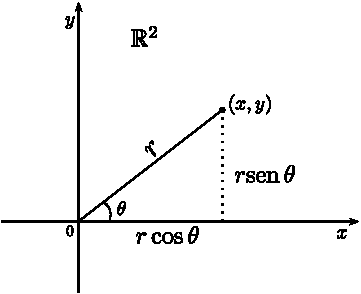
\includegraphics[scale=1.2]{Figuras/fig-coordenadas-polares}
\caption{A descrição em coordenadas polares de um número complexo $z=x+iy$.}
\label{fig-coord-polares}
\end{figure}

Daí segue que qualquer número complexo não-nulo $z=x+iy$ pode ser escrito como
$z=r(\cos\theta+i\sen\theta)$, onde $r=|z|=\sqrt{x^2+y^2}$. 
Esta é chamada de representação ou forma polar do número complexo $z$.
\index{Forma polar}
O ângulo $\theta$ da forma polar é chamado de \textit{um argumento} de $z$. 
Já que as funções seno e cosseno são funções periódicas de período $2\pi$ é 
natural pensar no angulo $\theta+2k\pi$, com $k\in\mathbb{Z}$, como 
também sendo um argumento de $z$. Para evitar este tipo de multiplicidade na determinação 
de um argumento é que restringimos acima as medidas de ângulos ao intervalo $[0,2\pi)$.
Desta maneira, cada número complexo não-nulo tem um argumento definido de forma única.
Mais a frente quando estivermos trabalhando com as funções exponencial e logaritmo 
complexo vamos discutir em detalhes o conceito de \textit{ramo do argumento}. 

Exemplificando, o número complexo $z=1+1i$ é identificado com o ponto $(1,1)\in\mathbb{R}^2$
que tem norma $\|(1,1)\|=\sqrt{2}$ e está localizado na bissetriz do primeiro quadrante 
sendo assim representado em coordenadas polares 
por $x=\sqrt{2}\cos(\pi/4)$ e $y=\sqrt{2}\sen(\pi/4)$.
Portanto a representação polar de $z=\sqrt{2}(\cos(\pi/4)+i\sen(\pi/4))$.


Vamos ver agora como fica a representação polar de um produto de dois números
complexos. Sejam $z,w\in\mathbb{C}$ cujas representações polares são dadas por
\begin{align*}
z = r(\cos\theta+i\sen\theta)\\
w = s(\cos\beta+i\sen\beta).
\end{align*}
Para obter a representação polar de $zw$ basta efetuar o produto destes dois números
em suas representações polares e usar as fórmulas bem conhecidas para seno e cosseno
da soma de dois ângulos como segue:
\begin{align}\label{eq-formula-prod-zw-coord-polares}
zw
&=
r(\cos\theta+i\sen\beta)s(\cos\beta+i\sen\beta)
\nonumber\\
&=
rs \big( (\cos\theta\cos\beta-\sen\theta\sen\beta) +i(\cos\theta\sen\beta+\sen\theta\cos\beta)\big)
\nonumber\\
&=
rs (\cos(\theta+\beta)+i\sen(\theta+\beta)).
\end{align}

É muito importante observar que $\theta+\beta$ não é necessariamente um argumento 
de $zw$, no sentido de que este ângulo pode estar fora do intervalo $[0,2\pi)$.
Isto poderia acontecer se os argumentos de $z$ e $w$ fossem, por exemplo, ambos
maiores que $\pi$. Veja o exemplo da figura abaixo:
\begin{figure}[h]
\centering
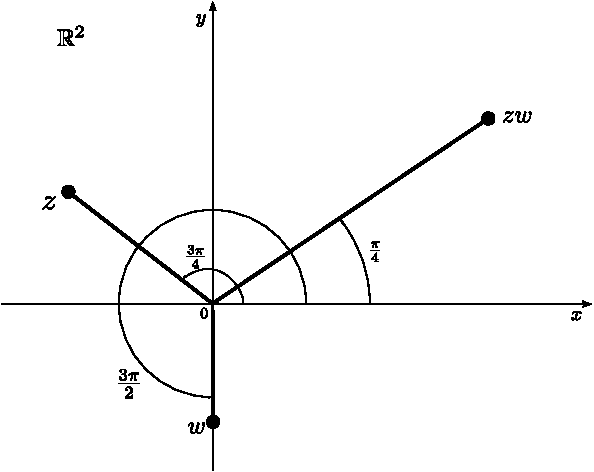
\includegraphics[scale=0.9]{Figuras/fig-prod-argumento}
\caption{Um argumento do produto $zw$}
\label{fig-coord-polares2}
\end{figure}

No exemplo da figura acima temos 
\begin{align*}
z=|z|(\cos(3\pi/4)+i\sen(3\pi/4))
\\[0.2cm]
w=|w|(\cos(3\pi/2)+i\sen(3\pi/2)).
\end{align*}
Aplicando a fórmula que deduzimos acima, ficamos com 
\[
zw=|z||w|(\cos(9\pi/4)+i\sen(9\pi/4)).
\]
Note que tudo está correto, mas como o ângulo que nossa fórmula para o produto fornece resulta em um valor 
maior que $2\pi$ quem de fato representará o argumento do produto $zw$, 
no intervalo anteriormente especificado $[0,2\pi)$, 
será o ângulo $\pi/4$, como mostrado na figura acima.

Este exemplo alerta para o fato de que, em geral, não é verdade que um argumento de um produto $zw$
é igual a soma dos argumentos de $z$ e $w$. Porém a menos de múltiplos inteiros de $2\pi$ isto 
é de fato verdadeiro. Mais a frente, quando apresentarmos a definição de ramo do argumento, 
de um número complexo $z$, que será denotado por $\mathrm{arg}(z)$, 
poderemos escrever esta última observação de modo mais sucinto através da notação abaixo
\[
\mathrm{arg}(zw) \equiv \mathrm{arg}(z)+\mathrm{arg}(w) \quad  (\mathrm{mod}\ 2\pi),
\] 
onde para qualquer $\alpha\in\mathbb{R}$ o símbolo $\alpha\ (\mathrm{mod}\ 2\pi)$
denota o único ângulo $\theta\in [0,2\pi)$ com a propriedade
que existe um único inteiro $k$ tal que $\theta +2k\pi= \alpha$.



Tomando $w=z$ em \eqref{eq-formula-prod-zw-coord-polares} obtemos
\[
z^2 = r^2(\cos(2\theta)+i\sen(2\theta)).
\] 
Esta igualdade sugere que as potencias sucessivas $z$ admite a seguinte representação
\[
z^n = r^n (\cos(n\theta)+i\sen(n\theta)), \quad \forall n\in\mathbb{N}.
\]
Esta afirmação é de fato verdadeira e pode ser facilmente obtida 
procedendo uma indução formal em $n$ e usando a identidade \eqref{eq-formula-prod-zw-coord-polares}.
Esta identidade é conhecida como Fórmula de De Moivre.
\index{Formula@Fórmula!De Moivre} 
Vamos usá-la no que segue para extrair 
raízes de um número complexo não-nulo arbitrário. 

Seja $w$ um número complexo não-nulo. Uma raíz $n$-ésima (ou de ordem $n$)
de $w$ é um número complexo $z$ satisfazendo a equação 
\[
z^n = w.
\]
Para procurar uma raíz $n$-ésima de $w$ vamos reescrever a equação acima 
usando coordenadas polares. Sejam $\beta\in [0,2\pi)$ um argumento de $w$ e $s=|w|$ 
a norma de $w$. Vamos escrever $z$ em coordenadas como $z=r(\cos\theta+i\sen\theta)$.
Pela Fórmula de De Moivre temos que $z^n=r^n(\cos(n\theta)+i\sen(n\theta))$.
Portanto 
\begin{align}\label{eq-aux-raiz-nesima-w}
z^n=w \quad \Longleftrightarrow \quad r^n(\cos(n\theta)+i\sen(n\theta)) = s(\cos\beta+i\sen\beta).
\end{align}
Tomando módulo dos dois lados da última igualdade acima, usando (I.7), $s>0$, $r\geqslant 0$ 
e que $|\cos\alpha+i\sen\alpha|=1$ para qualquer $\alpha\in\mathbb{R}$ temos que 
\begin{eqnarray*}
&|r^n(\cos(n\theta)+i\sen(n\theta))| = |s(\cos\beta+i\sen\beta)|&
\\[0.3cm]
&\Downarrow&
\\[0.3cm]
&r^n|\cos(n\theta)+i\sen(n\theta))| = s|(\cos\beta+i\sen\beta)|&
\\[0.3cm]
&\Downarrow&
\\[0.3cm]
&r^n=s.&
\end{eqnarray*}
Portanto $r = \sqrt[n]{s}$ e isto implica que qualquer solução $z$ da 
equação $z^n=w$ é tal que $|z|=  \sqrt[n]{s}$. Já que $s>0$ e $r^n=s$ podemos
concluir de \eqref{eq-aux-raiz-nesima-w} que o argumento $\theta$ de qualquer solução 
da equação satisfaz
$
\cos(n\theta)+i\sen(n\theta) = \cos\beta+i\sen\beta.
$
Já que dois números complexos são iguais se e somente se suas partes real e imaginária
coincidem, podemos afirmar que $\theta$ é solução do sistema não-linear
\[
\begin{cases}
\cos(n\theta)=\cos\beta
\\[0.1cm]
\sen(n\theta)=\sen(\beta).
\end{cases}
\]

Usando que as funções seno e cosseno são funções periódicas de período $2\pi$
concluímos que para cada $k\in\mathbb{Z}$ fixado o ângulo $\theta\equiv \theta(k,\beta)$ 
satisfazendo a igualdade $n\theta = \beta + 2k\pi$ é uma solução do sistema acima.
Para representar $z$ em coordenadas polares é preciso escolher dentre todas estas 
soluções apenas aquelas que satisfazem a condição $\theta\in [0,2\pi)$.
Desta forma só nos interessa os valores de $k$ para os quais 
temos 
\begin{align}\label{eq-aux2-raiz-nesima-w}
0\leqslant \frac{\beta}{n}+ \frac{2k\pi}{n}<2\pi. 
\end{align}
Lembrando que $\beta\in [0,2\pi)$ temos que 
\begin{align}\label{eq-aux3-raiz-nesima-w}
0\leqslant \frac{\beta}{n}<\frac{2\pi}{n}.
\end{align}
Usando a primeira desigualdade que aparece em \eqref{eq-aux2-raiz-nesima-w} e em seguida
a segunda desigualdade em \eqref{eq-aux3-raiz-nesima-w} obtemos a seguinte as seguintes desigualdades
\[
-\frac{2\pi k}{n}\leqslant \frac{\beta}{n}<\frac{2\pi}{n}
\quad \Longrightarrow \quad 
-\frac{2\pi k}{n}<\frac{2\pi}{n}
\quad \Longrightarrow \quad
\quad -k<1\quad 
\Longrightarrow \quad 
k>-1.
\]
Já que $k$ tem que ser um número inteiro então $k$ deve ser escolhido de forma que 
$k\geqslant 0$. 

Usando agora a segunda desigualdade em \eqref{eq-aux2-raiz-nesima-w} e a primeira 
desigualdade em \eqref{eq-aux3-raiz-nesima-w} temos que 
\[
\frac{\beta}{n}+ \frac{2k\pi}{n}<2\pi
\quad \Longrightarrow \quad 
\frac{2k\pi}{n}<2\pi-\frac{\beta}{n}
<
2\pi
\quad \Longrightarrow \quad 
2k\pi<2n\pi
\quad \Longrightarrow \quad 
k<n.
\]
Juntando esta restrição com a anterior podemos ver que devemos escolher $k\in \{0,1,2,\ldots,n-1\}$.


Desta forma cada um dos números complexos 
\begin{align}\label{eq-sol-ZN=w}
z_k = 
\sqrt[n]{s}
	\left(
		\cos\Big(\frac{\beta}{n}+ \frac{2k\pi}{n}\Big)+i\sen\Big(\frac{\beta}{n}+ \frac{2k\pi}{n}\Big)
	\right),
	\qquad 0\leqslant k\leqslant n-1
\end{align}
é uma solução de $z^n=w$. Como esta equação admite no máximo $n$ soluções e a lista acima 
possui exatamente $n$ elementos concluímos finalmente que os 
números $\{z_0,z_1,\ldots, z_{n-1}\}$ são todas as soluções possíveis desta equação. 


Um caso particular muito importante é o caso em que $w=1$. Neste caso as soluções da equação 
$z^n=1$ são chamadas de raízes $n$-ésimas da unidade. 
\index{Raízes da unidade}
Para $w=1$, temos $s=1$ e $\beta=0$. 
Logo fórmula das raízes $n$-ésimas obtida acima se reduz a 
\[
z_k = 
		\cos\Big(\frac{2k\pi}{n}\Big)+i\sen\Big(\frac{2k\pi}{n}\Big),
	\qquad 0\leqslant k\leqslant n-1.
\]
Este conjunto é chamado do conjunto das raízes $n$-ésimas da unidade. 
Ele pode ser também descrito, graças a Fórmula de De Moivre, 
de uma maneira ainda mais sucinta, isto é, como um conjunto de potências
sucessivas do número complexo 
$\omega = z_1 = $
isto é, $\{1,\omega,\omega^{2},\ldots,\omega^{n-1}\}$.


A título de exemplo vamos calcular as raízes cúbicas e quarta da unidade. 
Primeiro as raízes cúbicas da unidade. 
Usando a fórmula deduzida acima temos que as raízes cúbicas da unidade
são dadas por $\{1,\omega,\omega^2\}$, onde 
\[
\omega 
= 
\cos\Big(\frac{2\pi}{3}\Big)+i\sen\Big(\frac{2\pi}{3}\Big)
=
-\frac{1}{2}+i\frac{\sqrt{3}}{2}
\]
e pela Fórmula de De Moivre 
\[
\omega^2
= 
\cos\Big(\frac{4\pi}{3}\Big)+i\sen\Big(\frac{4\pi}{3}\Big)
=
-\frac{1}{2}-i\frac{\sqrt{3}}{2}.
\]

Para calcular as raízes quartas da unidade basta proceder como acima, mas 
observando que agora o conjunto é dado por $\{1,\omega,\omega^2,\omega^3\}$,
com $\omega$ neste caso dado por 
\[
\omega 
= 
\cos\Big(\frac{2\pi}{4}\Big)+i\sen\Big(\frac{2\pi}{4}\Big)
=
i.
\]
Logo $\omega^2 = i^2 =-1$ e $\omega^{3}=-i$.

\begin{figure}[h]
\centering
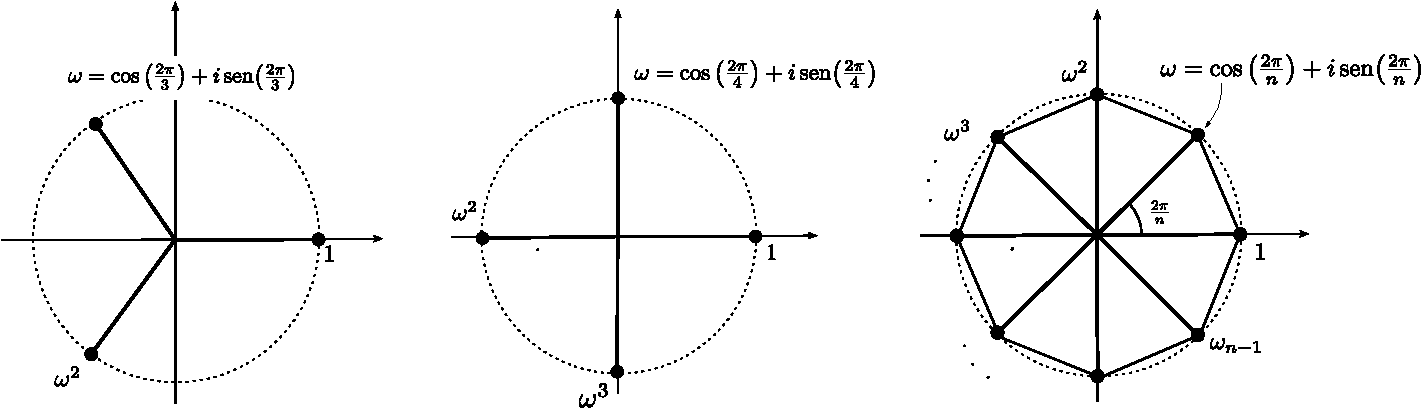
\includegraphics[scale=0.6]{Figuras/raizes-da-unidade}
\caption{Primeira figura representa as raízes cúbicas da unidade, a segunda as raízes quartas da unidade, e a última
o caso geral das raízes $n$-ésimas da unidade.}
\label{fig-raizes-unidade}
\end{figure}

\break 

Para finalizar esta seção observamos que as raízes $n$-ésimas da unidade 
determina o conjunto de vértices de um polígono regular $n$ lados inscrito 
no círculo de centro zero e raio um, como mostrado na Figura \ref{fig-raizes-unidade}.

%%%% Para escrever os apendices basta usar os comandos abaixo.
\begin{subappendices}
\markboth{Ap\^{e}ndice 1}{Ap\^{e}ndice 1}

Esta seção é baseada em um dos volumes da fantástica coleção de livros de Análise 
escritas por Barry Simon. Fora o exemplo que é totalmente desenvolvido aqui 
as demais informações seguem de perto a exposição de Barry Simon e
podem ser encontradas no Capítulo 1 da referência \cite{MR3443339}.



\section{Observações Históricas}
O uso de expressões como ``imaginário'' e ``complexo'' atestam que o processo de aceitação 
dos números complexos foi bastante difícil. Podemos pensar que, 
dada a fórmula para soluções da equação quadrática, que raízes quadradas 
de números negativos tivessem um passado muito antigo. 
Muitos imaginam que a motivação para se introduzir números complexos
tenha vindo de tempos antigos e de pessoas 
que se sentiam desconfortáveis com o fato de equações como $x^2+1=0$ 
não ter solução. A verdade é que os números complexo vieram mesmo do estudo 
de equações cúbicas, da forma 
\[
x^3-ax-b=0.
\]
Em 1515, Scipione del Ferro (1465-1526) deduziu que 
\begin{align}\label{formula-del-Ferro}
x
=
\sqrt[3]{ \frac{b}{2} +  \sqrt[2]{ \frac{b^2}{4}-\frac{a^3}{27} }  }
+
\sqrt[3]{ \frac{b}{2} -  \sqrt[2]{ \frac{b^2}{4}-\frac{a^3}{27} }  }
\end{align}
era uma solução desta cúbica, mas nunca publicou sua descoberta.
O mais intrigante e que mesmo em casos onde 
\begin{align}\label{eq-aux1-del-Ferro} 
\frac{b^2}{4}-\frac{a^3}{27}<0
\end{align}
a solução de del Ferro fornecia, depois de simplificada, um número real como solução da cúbica!

Um caso muito particular mas que ilustra bem como deve ter sido desafiante para del Ferro 
entender o que estava acontecendo é o caso em que tomamos $b=2$ e $a=3\sqrt[3]{2}$.
Estes valores foram escolhidos para fazer com que a expressão do lado esquerdo da desigualdade \eqref{eq-aux1-del-Ferro}
seja exatamente $-1$ e portanto
\[
x =
\sqrt[3]{1+\sqrt[2]{(-1)}}
+
\sqrt[3]{1-\sqrt[2]{(-1)}}
\]
O que obviamente era uma expressão que del Ferro, na época, deveria considerar muito intrigante,
principalmente porque o número $x$ que aparece acima (apesar desta representação complexa) 
é na realidade um número real! Vamos provar este 
fato abaixo, porém, usando ferramentas do século XX.

Primeiro precisamos fazer uma escolha para $\sqrt[2]{(-1)}$. A escolha mais 
natural hoje em dia é definir este número como sendo uma das duas soluções distintas da equação $z^2=-1$. 
Na seção anterior vimos como calcular as raízes desta equação e que elas são dadas por 
$z=i$ e $z=-i$.
A simetria presente na expressão de del Ferro fará com que o valor $x$ seja o mesmo para qualquer uma 
das duas escolhas $\sqrt[2]{(-1)}=i$ 
ou $\sqrt[2]{(-1)}=-i$.
Por simplicidade vamos tomar $\sqrt{(-1)}=i$. Substituindo na expressão acima 
ficamos com 
\[
x =
\sqrt[3]{1+i}
+
\sqrt[3]{1-i}.
\]
Raciocinando de maneira análoga, podemos definir $\sqrt[3]{1+i}$ 
como sendo (na notação da seção anterior) a solução $z_0$ da equação $z^3=1+i$. 
Para isto basta escrever $1+i$ em coordenadas polares $1+i = \sqrt{2}(\cos\pi/4+i\sen\pi/4)$
e usar a fórmula dada para $z_0$, obtendo a seguinte expressão:
\[
\sqrt[3]{1+i} = (\sqrt{2})^{\frac{1}{3}}\Big(\cos\big(\frac{\pi}{12}\big)+i\sen\big(\frac{\pi}{12})\Big)
\]
Repetimos o mesmo procedimento para $\sqrt[3]{1-i}$. 
Novamente, para encontrar a solução $z_0$ da equação $z^3=1-i$ primeiro escrevemos $1-i$ em coordenadas polares
$1-i = \sqrt{2}\big(\cos(7\pi/4) +i\sen(7\pi/4)\big)$. Depois aplicamos a fórmula para $z_0$ e temos
que 
\[
\sqrt[3]{1-i} = (\sqrt{2})^{\frac{1}{3}}\Big(\cos\big(\frac{7\pi}{12}\big)+i\sen\big(\frac{7\pi}{12})\Big).
\]

Já que os senos que aparecem nas duas expressões em destaque acima, quando somados, 
se anulam e os cossenos têm o mesmo valor descobrimos que 
\[
x= 
2\sqrt[6]{2}\cos\big(\frac{\pi}{12}\big) 
= 
2\sqrt[6]{2}\cdot \frac{1+\sqrt{3}}{2\sqrt{2}}
=
\frac{1+\sqrt{3}}{\sqrt[3]{2}}.
\]

Com esta raíz em mãos é simples descobrir quais são as outras duas, basta 
aplicar o algoritmo da divisão de polinômios e em seguida a Fórmula de Bhaskara. 
Feito isto descobrimos que todas as suas raízes são reais e dadas por
\[
x= \frac{1+\sqrt{3}}{\sqrt[3]{2}},\quad 
x= -\sqrt[3]{4} \quad \text{e}\quad x= \frac{1-\sqrt{3}}{\sqrt[3]{2}}.
\]

A fórmula de del Ferro \eqref{formula-del-Ferro} foi publicada em um livro de Girolamo Cardano (1501-1576) em 1545.
Apesar do livro de Cardano ter exemplos onde $b^2/4-a^3/27<0$ ele nunca aplicou 
a fórmula neste casos!


Vinte e sete anos mais tarde, Rafael Bombelli (1526-1572) publicou um livro
que continha instruções do que viria a ser no futuro as regras da aritmética no 
conjunto dos números complexo e as usou para encontrar raízes reais de cúbicas
a partir da fórmula de del Ferro. A publicação chave para deslanchar a teoria
dos números complexos foi o trabalho de Wallis e Euler que apareceram por volta de 1748.
Em particular, nesta época Euler esclarece como deveriam ser entendidas as raízes da unidade.
Usando suas técnicas ele mostra que \eqref{formula-del-Ferro} 
era uma fórmula que na verdade representa não apenas uma, mas em diversos casos 
várias das raízes da cúbica. Mesmo após estas grandes descobertas ainda foram necessários
mais cem anos para a comunidade matemática aceitar completamente os números complexos.
Assim muito do trabalho de Cauchy (que é um dos pais fundadores da teria do cálculo integral e diferencial
de funções complexas) foi realizado em uma atmosfera em que mesmo o próprio Cauchy não se sentia muito 
confortável. 

O ponto de vista geométrico dos números complexos, como pontos do plano Euclidiano, 
foi introduzido por Jean-Robert Argand(1768-1822) e Caspar Wessel (1745-1818) e defendida
por Gauss. Argand e Wessel não eram matemáticos profissionais. Wessel era um agrimensor
e apresentou sua interpretação geométrica para a Acadêmia Real Dinamarquesa em 1797.
Em seguida, em 1799 seu trabalho foi publicado e pouco depois esquecido e não teve
nenhum impacto. Mais tarde a abordagem geométrica foi redesenvolvida por 
dois matemáticos dinamarqueses Sophus Christian Juel e o famoso Sophus Lie.

Argand era um contador e livreiro, e em 1806 publicou por conta própria seu 
trabalho em um livro que apareceu sem o seu nome! Em 1813 um matemático Francês,
Jacques Français, publicou um artigo que dava sequência ao trabalho de Argand,
onde ele solicitou que o autor do misterioso livro se revelasse. Desta forma 
Argand recebeu reconhecimento por seu trabalho e figuras 
geométricas como as da Figura \ref{fig-coord-polares} são frequentemente chamadas de diagramas
de Argand. 



\end{subappendices}

% Lista 1
%\chapter*{Lista 1}
\addcontentsline{toc}{chapter}{Lista 1}
\markboth{Lista 1}{Lista 1}
%%%%%%%%%%%%%%%%%%%%%%%%%%%%%%%%%%%%%%%%%%%%%%%%




% Inicio da Lista de Exercícios 
\begin{enumerate}[leftmargin=*]

	\item Reduza à forma $x+iy$
	\begin{itemize}
		\item[a)] $(1-5i)^2-4i$;
		\item[b)] $-i(-1+i)+2$;
		\item[c)] $(3+i)(1-11i)$;
		\item[d)] $(\sqrt{2}-i\sqrt{5})(\sqrt{5}+i\sqrt{2})$;
	\end{itemize}
	\item Novamente reduza à forma $x+iy$ 
	\begin{itemize}
		\item[a)] $\displaystyle\frac{3-4i}{2i}$;\\
		\item[b)] $\displaystyle\frac{2+5i}{-1+i\sqrt{3}}$;\\
		\item[c)] $\displaystyle\frac{(2-2i)^2}{1+i}$;\\
		\item[d)] $\displaystyle\frac{z-\overline{z}i}{\overline{z}-zi}$;\\[-0.3cm]
	\end{itemize}
	\item Faça o esboço e identifique os seguintes conjuntos 
	\begin{itemize}
		\item[a)] $|z|=|z-2|$;
		\item[b)] $|z|=|\overline{z}-1|$;
		\item[c)] $a|z|=|z-1|$, com $a\in\mathbb{R}\setminus\{0,1\}$;
		\item[d)] $\Re(z)=\Im(z-1)$;
		\item[e)] $\Im(z-1)=|z+1|$;
		\item[f)] $|\overline{z}|=|z-1|$;
	\end{itemize}
	\item Usando a primeira desigualdade triangular, mostre que $||z_1|-|z_2||\leq |z_1-z_2|$.
	\item Deduza a desigualdade $|z_1+z_2+z_3|\leq |z_1|+|z_2|+|z_3|$.
	\item Mostre que, se $z_2\neq -z_3$ então $\displaystyle\left|\frac{z_1}{z_2+z_3}\right|\leq \frac{|z_1|}{||z_2|-|z_3||}$.\\
	\item Resolva as equações\\ a) $z-\overline{z}=1$;\\ b) $z+\overline{z}i=2+i$;\\ c) $z+2\overline{z}=1-i$.
	\item Mostre que $|z_1+z_2|< |1+\overline{z_1}z_2|$, desde que $|z_1|< 1$ e $|z_2|<1$.
	\item Encontre todas as soluções das equações\\ a) $z^2=1-i\sqrt{3}$;\\ b) $z^5=-1$;\\ c) $\overline{z}^3=1$;\\ d) $z^7=-(1+i)$.
	\item Seja $P(x)=ax^2+bx+c$ um polinômio de grau 2 com coeficientes reais e suponha que $\Delta=b^2-4ac<0$. Então 
	as soluções da equação $P(x)=0$ são números complexos com parte imaginária não nula. Se $z_1$ e $z_2$ são estas soluções,
	mostre que $z_1=\overline{z_2}$. Mais geralmente, se $P(x)=a_nx^n+a_{n-1}x^{n-1}+\ldots+a_1x+a_0$ é um polinômio de 
	grau $n>0$ arbitrário, com coeficientes reais, e se $z_0\in \mathbb{C}$ é tal que $P(z_0)=0$, então tem-se que 
	$P(\overline{z_0})=0$. 
	\item Considere a equação $az^2+bz+c=0$, onde $a,b$ e $c\in \mathbb{C}$. Deduza uma expressão para suas raízes.
	\item Deduza a fórmula $1+z+z^2+\ldots+z^{n-1}=\displaystyle\frac{1-z^n}{1-z}$, se $z\neq 1$.
	\item Use o exercício anterior para mostrar que se $\omega\neq 1$, satisfaz a equação $\omega^n=1$, então 
	$1+\omega+\omega^2+\ldots+ \omega^{n-1}=0$.
	\item Demonstre a fórmula De Moivre 
	$$
	(\cos\theta+i\,\text{sen}\, \theta)^n=\cos n\theta+i\,\text{sen}\, n\theta.
	$$
	\item Usa o exercício anterior para mostrar que \\
	a) $\cos 2\theta =\cos^2\theta-\sen^2\theta$;\\
	b) $\sen 2\theta =2\,\sen\theta\cos\theta$;\\
	c) $\cos 3\theta =\cos^3\theta-3\cos\theta\, \sen^2\theta$;\\
	d) $\sen 3\theta =3\cos^2\theta\,\sen\theta-\sen^3\theta$.
	\item Use o exercício anterior para deduzir expressões para 
	$\sen 4\theta$ e $\cos 4\theta$.
	\item Calcule $(2+i)(3+i)$ e deduza a igualdade 
	$$
	\frac{\pi}{4}=\arctan\left( \frac{1}{2}\right)+\arctan\left( \frac{1}{3}\right).
	$$
	\item Calcule $(5-i)^4(1+i)$ e deduza a igualdade 
	$$
	\frac{\pi}{4}=4\arctan\left( \frac{1}{5}\right)-\arctan\left( \frac{1}{239}\right).
	$$
	\item Mostre que três pontos $a,b$ e $c$ no plano complexo são colineares, se e somente se, 
	$$
	\det\begin{bmatrix}
	    	1\ &a\ &\overline{a}\ \\
	    	1\ &b\ &\overline{b}\ \\
	    	1\ &c\ &\overline{c}\ 
	    \end{bmatrix}=0.
	$$


	\item Uma maneira de definir uma ordem ``$<$'' em um corpo $\mathscr{C}$ 
	consiste um dar um subconjunto $\mathscr{C}^+$ de 
	$\mathscr{C}$ tal que: 
	\begin{itemize}
		\item[i)] se $x,y\in\mathscr{C}^+$ então $x+y\in\mathscr{C}^+$ e $xy\in\mathscr{C}^+$ 
		(o conjunto $\mathscr{C}^+$ é chamado de conjunto dos números positivos);
		\item[ii)] dado $x\in\mathscr{C}$ então apenas uma das possibilidades se verifica: 
		ou $x\in\mathscr{C}^+$, ou $x=0$ ou $-x\in\,\mathscr{C}^+$.  
	\end{itemize}
	Em seguida dizemos que $x<y$ se e somente se $y-x\in \mathscr{C}^{+}$.
	Note que segue das propriedades i) e ii) que o quadrado de 
	qualquer elemento não-nulo de $\mathscr{C}$ é um elemento do subconjunto dos positivos.
	De fato, se $x\in\mathscr{C}^+$ então $x^2\in\mathscr{C}^+$ por i). Por outro lado, se $-x\in\mathscr{C}$ então 
	 $(-x)^2=(-x)(-x)=x^2\in \mathscr{C}^+$, por i) novamente. Conclua que o corpo $\mathbb{C}$ 
	 não pode admitir nenhuma ordem do tipo definido acima.
	
	
	

\end{enumerate}
%  Fim da Lista de Exercícios





% Semana 2 
% !TeX spellcheck = pt_BR
%\chapter[Semana 2]{}
\chapter[Noções de Topologia]{Noções de Topologia}
\chaptermark{}


\hfill%
\begin{minipage}{14cm}
\begin{flushright}
\rightskip=0.5cm
\textit{``Talk with M. Hermite. He never evokes a concrete image, yet you soon perceive that: the more abstract entities are to him like living creatures.''}
\\[0.1cm]
\rightskip=0.5cm
---Henri Poincare
\end{flushright}
\end{minipage}

\section{Noções de Topologia no Plano Complexo}\label{sec-nocoes-top}

Nesta seção vamos apresentar de forma mais simples possível alguns conceitos topológicos necessários 
para desenvolvimento da teoria de funções contínuas e deriváveis de uma variável complexa.
A abordagem adotada aqui não é a mais geral possível, como feita em livros de topologia, mas sim 
baseada nos textos sobre Espaços Métricos. Uma boa referência para uma exposição mais completa 
sobre os aspectos métricos e a topologia de $\mathbb{C}$ é o Capítulo II da referência 
\cite{MR503901}. A vantagem desta abordagem é que a grande maioria dos conceitos topológicos
podem ser apresentados usando sequências. 

\subsection{Convergência de Sequências de Números Complexos}

Dizemos que uma sequência $\{z_1,z_2,\ldots\}$, notação $(z_n)_{n\in\mathbb{N}}$, 
de números complexos converge para um número complexo 
\index{Sequência!convergente}
$w\in\mathbb{C}$ se 
\[
\lim_{n\to\infty} |z_n-w| = 0 \qquad\text{e escrevemos}\qquad \lim_{n\to\infty}z_n = w.
\]
Em alguma ocasiões vamos optar também por uma das seguintes notações alternativas 
para nos referir ao limite acima: 
\begin{itemize}
	\item $z_n\to w$, quando $n\to\infty$;
	\item $z_n\xrightarrow{n\to\infty}w$.
\end{itemize}

Observamos que esta noção de convergência não é nova, já que o módulo em $\mathbb{C}$
coincide com a distância Euclidiana em $\mathbb{R}^2$. Isto quer dizer que olhando para 
$z_n$ e $w$ como pontos de $\mathbb{R}^2$ a condição $|z_n-w|\to 0$ se traduz no fato
que a distância entre os elementos da sequência $z_n$ e $w$ em $\mathbb{R}^2$ 
fica arbitrariamente pequena quando $n$ tende a infinito. 

Para os mais aficionados pelas definições matematicamente rigorosas a noção de convergência
apresentada acima pode se definida como segue.

\begin{definicao}[Limite de uma sequência]\label{def-limite-seq}
\index{Limite!de uma sequência}
Dizemos que uma sequência de números complexos $(z_n)_{n\in\mathbb{N}}$ converge para um número 
complexo $w\in \mathbb{C}$ se para cada $\epsilon>0$ dado, existe $N_0\in\mathbb{N}$ 
(que pode depender de $\varepsilon$) tal que para todo $n\geqslant N_0$ temos 
$|z_n-w|<\varepsilon$. 
\end{definicao}

\begin{figure}[h]
\centering
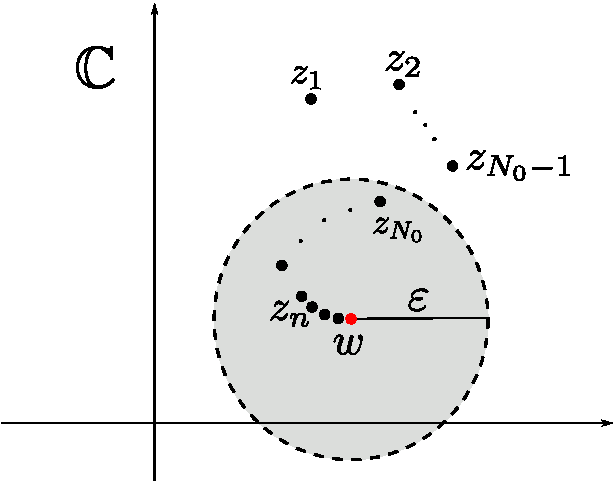
\includegraphics[scale=0.6]{Figuras/fig-sequencia-convergente}
\caption{Definição de limite de uma sequência. Neste figura podemos ver que para $\varepsilon>0$ escolhido, todos os elementos da sequência $(z_n)_{n\in\mathbb{N}}$ cujos índices são maiores ou iguais a um certo $N_0$, são tais que a distância deles à $w$ é menor do que $\varepsilon$.}
\label{fig-sequencia-cauchy1}
\end{figure}


Uma observação importante. 
Já que o objetivo deste texto é ser um texto introdutório à teoria de funções de uma variável complexa, 
vamos evitar ao máximo trabalhar com a definição rigorosa de limite dada acima. Em alguns poucos 
casos, em que isto não for possível, fornecemos figuras ilustrando os argumentos ou conceitos de forma que 
o leitor seja capaz de absolver boa parte das ideias envolvidas.
 
\begin{lema}
\label{lema-conv-parte-real-im-seq}
Seja $(z_n)_{n\in\mathbb{N}}$ é uma
sequência em $\mathbb{C}$. A sequência $z_n\to w$, quando $n\to \infty$, se e somente
se, as sequências de números reais $(\Re(z_n))_{n\in\mathbb{N}}$ e $(\Im(z_n))_{n\in\mathbb{N}}$ convergem, quando $n\to\infty$. Além do mais,
\[
\lim_{n\to\infty} \Re(z_n) = \Re(w)
\qquad \text{e} \qquad 
\lim_{n\to\infty} \Im(z_n) = \Im(w).
\]
\end{lema} 
%\begin{proof}
%A prova deste lema é uma simples aplicação do 
%Lema \ref{lema-re-im-modulo}, da Desigualdade Triangular (Teorema \ref{teo-des-triang})
%e da identidade (I.7) (página \pageref{page:eq-prop-basicas-conjugado}).

%Primeiro assumimos que $z_n\to w$,
%quando $n\to\infty$. 
%Neste caso, temos que 
%\begin{align*}
%\left| 
%\Big(\lim_{n\to\infty}\Re(z_n)\Big) -\Re(w)
%\right|
%&=
%\left| 
%\lim_{n\to\infty}\big(\Re(z_n) -\Re(w)\big)
%\right|
%\\[0.2cm]
%&=
%\lim_{n\to\infty}|\Re(z_n)-\Re(w)|
%\\[0.2cm]
%&=
%\lim_{n\to\infty}|\Re(z_n-w)|
%\\[0.2cm]
%&\leq 
%\lim_{n\to\infty}|z_n-w|
%=
%0,
%\end{align*}
%onde na terceira igualdade usamos que para todo $z,w\in\mathbb{C}$ temos
%$\Re(z)-\Re(w) = \Re(z-w)$. Analogamente provamos a convergência da 
%sequência das partes imaginárias. 

%Reciprocamente, vamos supor que $\Re(z_n)\to a$ e $\Im(z_n)\to b$,
%quando $n\to\infty$. Seja $w=a+ib$. Então para todo $n\in\mathbb{N}$
%temos a seguinte desigualdade 
%\begin{align*}
%|z_n-w|
%&=
%|\Re(z_n)+i\,\Im(z_n) - (a+ib)|
%\\
%&=
%|(\Re(z_n)-a)+i(\Im(z_n)-b)|
%\\
%&\leqslant
%|(\Re(z_n)-a)|+|i(\Im(z_n)-b)|
%\\
%&\leqslant
%|\Re(z_n)-a|+|\Im(z_n)-b|.
%\end{align*} 
%Portanto tomando o limite em ambos os lados verificamos que 
%\[
%\lim_{n\to\infty}|z_n-w|
%\leqslant 
%\lim_{n\to\infty}|\Re(z_n)-a| + 
%\lim_{n\to\infty}|\Im(z_n)-b|
%=0.
%\]

%\end{proof}

Uma grande dificuldade que enfrentamos para trabalhar com o conceito de limite é que, em geral,
não é fácil determinar o ponto para onde nossa sequência converge, mesmo sabendo \textit{a priori} que ela é 
convergente. Por esta razão é conveniente ter em mãos outras condições equivalente para facilitar nossa
tarefa. Uma das mais famosas e utilizadas caracterizações de convergência é a 
de sequências de Cauchy. 

\begin{definicao}\label{def-seq-Cauchy}
\index{Sequência!de Cauchy}
Dizemos que uma sequência $(z_n)_{n\in\mathbb{N}}$ é uma sequência de Cauchy se 
para todo $\varepsilon>0$ dado existe $N_0\in\mathbb{N}$ tal que para todo $m,n\geqslant N_0$
temos 
\[
|z_n-z_m|<\varepsilon.
\]
\end{definicao}
\begin{figure}[h]
\centering
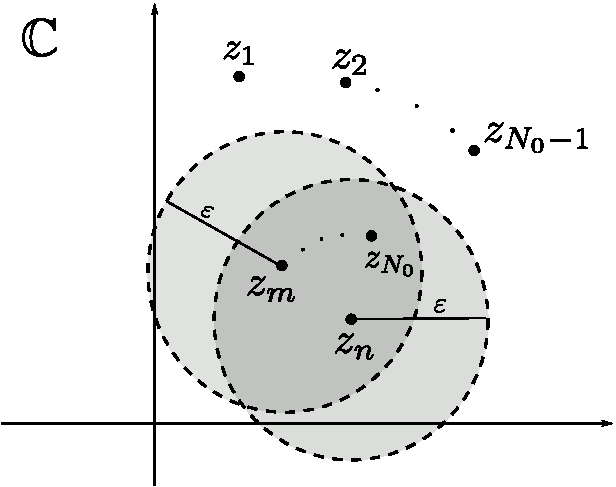
\includegraphics[scale=0.6]{Figuras/fig-sequencia-Cauchy-2}
\caption{Sequência de Cauchy. Segundo a definição para uma sequência ser uma sequência de Cauchy dado $\varepsilon>0$
é possível encontrar um índice $N_0$ tal que se $m$ e $n$ são ambos maiores ou iguais a $N_0$ então 
a distância entre $z_n$ e $z_m$ é no máximo $\varepsilon$. Em outras palavras, para índices suficientemente
grandes os todos os elementos estarão $\varepsilon$-próximos um dos outros.}
\label{fig:fig-sequencia-cauchy}
\end{figure}


Um fato muito importante sobre o conjunto dos números reais é que ele munido de suas operações usuais 
forma um \textit{corpo ordenado} e \textit{completo}.
O adjetivo completo, significa que toda sequência de Cauchy de números reais é convergente
e vice-versa. Como consequência de $\mathbb{R}$ ser completo e das
partes reais e imaginárias serem limitadas por $|z|$, 
segue que $\mathbb{C}$ também é completo. 
De fato, seja $(z_n)_{n\in\mathbb{N}}$ uma sequência de Cauchy em $\mathbb{C}$.  
Nosso primeiro passo é mostrar que a limitação das partes real
e imaginária pode ser usada para mostrar
que as sequências de números reais $(\Re(z_n))_{n\in\mathbb{N}}$ e $(\Im(z_n))_{n\in\mathbb{N}}$
são sequências de Cauchy em $\mathbb{R}$. Já que $(z_n)_{n\in\mathbb{N}}$ uma sequência de Cauchy em $\mathbb{C}$,
sabemos que para qualquer $\varepsilon>0$, existe um $N_0\in\mathbb{N}$ tal que para todo $n,m\geqslant N_0$
temos $|z_n-z_m|<\varepsilon$. Pela limitação das partes real
e imaginária, temos então que 
\begin{align*}
|\Re(z_n)-\Re(z_m)| = |\Re(z_n-z_m)|\leqslant |z_n-z_m|<\varepsilon
\\[0.2cm]
|\Im(z_n)-\Im(z_m)| = |\Im(z_n-z_m)|\leqslant |z_n-z_m|<\varepsilon.
\end{align*}
Mostrando que as partes real e imaginária da sequência $(z_n)_{n\in\mathbb{N}}$ são 
ambas sequências de Cauchy. Como $\mathbb{R}$ é completo então cada uma destas sequências 
é convergente, isto é, existem $x,y\in\mathbb{R}$ tais que 
\[
x=\lim_{n\to\infty} \Re(z_n) \qquad \text{e}\qquad 
y=\lim_{n\to\infty} \Im(z_n).
\]
Ainda resta mostrar que $z_n$ converge para $z=x+iy$, quando $n\to\infty$. 
Mas para basta aplicar o Lema \ref{lema-conv-parte-real-im-seq}.

\subsection{Topologia no Plano Complexo}

Vamos voltar nossa atenção agora para alguns conceitos topológicos que serão necessários
para o desenvolvimento do nosso estudo. A maioria das conceitos deve ser razoavelmente 
familiar para a maioria dos estudantes de cálculo e portanto não serão muito novos e
podem ser visto apenas como os antigos mas apresentados em um novo vocabulário. 


\medskip 

Dado um ponto $z\in\mathbb{C}$ e $r>0$ definimos o {\bf disco aberto} de centro 
$z$ e raio $r$, notação $D(z,r)$,
como sendo o conjunto de todos os números complexos que estão a distância no máximo $r$ de $z$,
isto é, $D(z,r) \equiv \{w\in\mathbb{C}: |z-w|<r \}$.
\index{Disco!aberto}
Definimos o {\bf disco fechado} de centro $z$ e raio $r$, notação $\overline{D}(z,r)$, 
como sendo o conjunto de todos os números complexos que estão a distância menor ou igual a $r$ 
do número complexo $z$, isto é, $\overline{D}(z,r)\equiv \{w\in\mathbb{C}: |w-z|\leqslant r\}$.
\index{Disco!fechado}
A fronteira de ambos $D(z,r)$ e $\overline{D}(z,r)$ é definida como sendo o conjunto 
de todos os pontos do plano complexo que estão a distância exatamente $r$ do ponto $z$,
isto, $\{w\in \mathbb{C}: |w-z|=r\}$. Este conjunto será denotado, em geral, por $\partial D(z,r)$, 
mas caso seja conveniente também podemos denotá-lo por $\partial \overline{D}(z,r)$. 
Como o disco aberto de centro zero e raio um irá desempenhar um papel de destaque neste texto,
vamos reservar uma notação especial para este conjunto. Ao invés de usar a notação $D(0,1)$
vamos nos referir a este disco pela notação $\mathbb{D}$, isto é $\mathbb{D}\equiv \{w\in \mathbb{C}: |w|<1\}$.
O conjunto $\mathbb{D}$ também será chamado as vezes de disco unitário.
\index{Disco!unitário}


\begin{figure}[h]
\centering
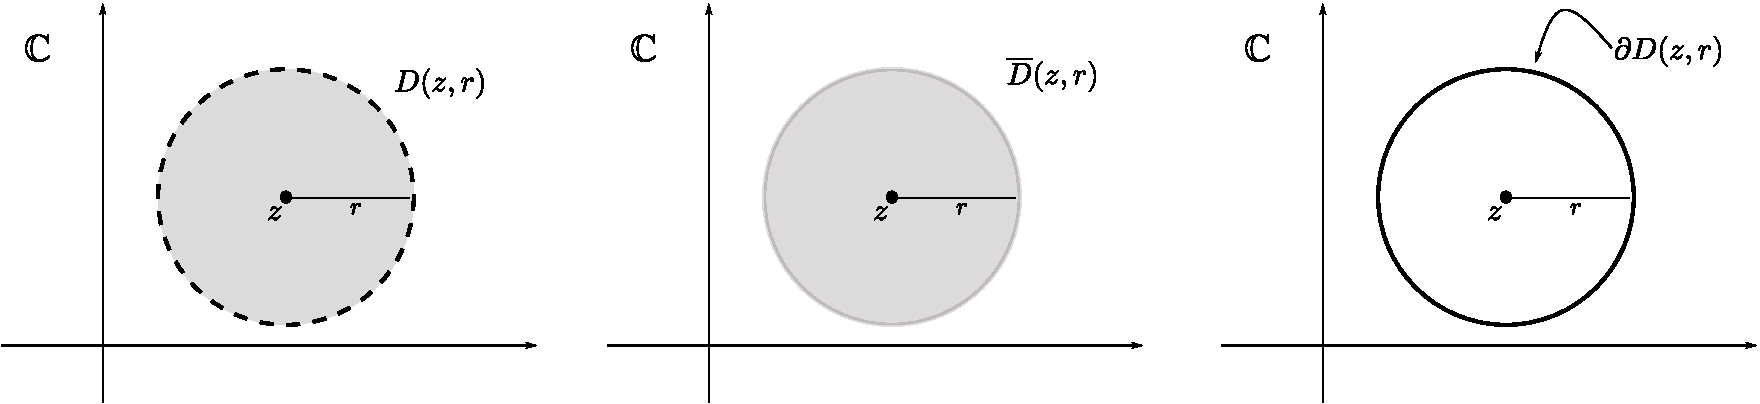
\includegraphics[width=1\linewidth]{Figuras/discos-fronteira}
\caption{Os dicos abertos e fechados de centro $z$ e raio $r>0$ e a fronteira destes discos.}
\label{fig:discos-fronteira}
\end{figure}


\medskip 

Dado um conjunto $U\subset \mathbb{C}$ vamos dizer que $z\in U$ é um {\bf ponto interior} de $U$
\index{Ponto!interior}
se existe algum $r>0$ tal que o disco aberto $D(z,r)$ esteja inteiramente contido em $U$ ou 
em outras palavras $D(z,r)\subset U$. 
O conjunto de todos os pontos interiores de $U$
\index{Interior!de um conjunto}
será denotado por $\mathrm{int}(U)$ e chamado de \textbf{interior de} $U$.
Dizemos que um conjunto $U\subset \mathbb{C}$ é um {\bf conjunto aberto} se todo ponto $z\in U$ é 
\index{Conjunto!aberto}
um ponto interior de $U$. 
Equivalentemente, um subconjunto $U\subset\mathbb{C}$ é aberto se, e somente se, 
$\mathrm{int}(U)=U$.

\begin{figure}[h]
\centering
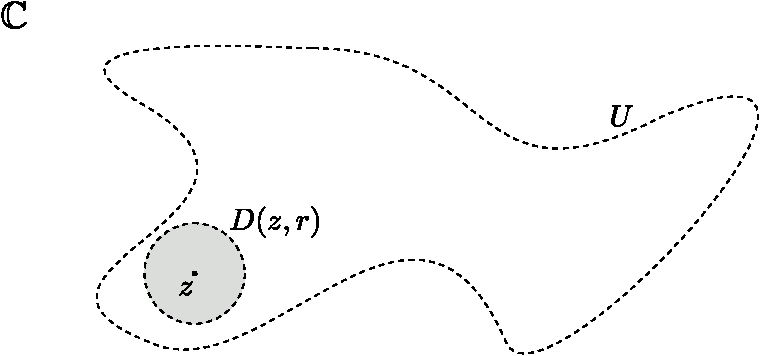
\includegraphics[scale=0.8]{Figuras/ponto-interior}
\caption{Nesta figura $z$ representa um ponto interior de um subconjunto $U\subset \mathbb{C}$.}
\label{fig:ponto-interior}
\end{figure}


Observe que esta definição de conjunto aberto do plano complexo é totalmente semelhante a definição de 
conjunto aberto em $\mathbb{R}^2$. É conveniente usar a convenção que o conjunto vazio é um conjunto aberto.
Observamos que existem diversos subconjuntos $B\subset \mathbb{C}$ com interior vazio, isto é, 
$\mathrm{int}(B)=\empty$. Mesmo assim é sempre verdade que $\mathrm{int}(B)$ é um conjunto
aberto, qualquer que seja $B\subset \mathbb{C}$. 

\medskip 

Um conjunto $F\subset V$ é dito {\bf conjunto fechado} se seu 
complementar $F^c\equiv \mathbb{C}\setminus F \equiv \{z\in \mathbb{C}: z\notin F\}$
\index{Conjunto!fechado}
é um conjunto aberto. 
Já que convencionamos que o conjunto vazio é aberto e já que todo o plano complexo $\mathbb{C}$
também é um conjunto aberto, então o complementar do vazio que é igual a todo plano complexo $\mathbb{C}$ é
um conjunto fechado; bem como o complementar de $\mathbb{C}$ que é igual ao conjunto vazio também é um conjunto
fechado. Podemos mostrar que os únicos subconjuntos de $\mathbb{C}$ que são simultaneamente abertos e fechados
são apenas: $\emptyset$ (conjunto vazio) e $\mathbb{C}$.

Um fato muito importante sobre os conjuntos fechados de $\mathbb{C}$ é que eles 
podem ser completamente caracterizados por sequências. Para isto precisamos de mais uma definição.
Um ponto $z\in\mathbb{C}$ é chamado de {\bf ponto de acumulação}\index{Ponto!de acumulação} de
um subconjunto $B\subset\mathbb{C}$ se existe uma sequência $(z_n)_{n\in\mathbb{N}}$
tal que para todo $n\in\mathbb{N}$ temos: $z_n\in B$ e $z_n\to z$,
quando $n\to\infty$. 


Um ponto $z\in B$ é chamado de {\bf ponto isolado}\index{Ponto!isolado} 
se existe algum $r>0$ de forma que $D(z,r)\cap B = \{z\}$. Ou seja um ponto $z$ de um conjunto $B$
é um ponto isolado se existe um disco de centro em $z$ e raio $r>0$ tal que 
o único ponto de $B$ que está dentro deste disco aberto é o próprio ponto $z$.

\begin{proposicao}\label{prop-caract-fechados-sequencias}
Um subconjunto não-vazio $F\subset\mathbb{C}$ é um conjunto fechado se, e somente se, todo ponto 
de acumulação de $F$ pertence a $F$. 
\end{proposicao}
Já que o complementar de um conjunto fechado é um conjunto aberto segue da proposição 
acima que os conjuntos abertos também podem ser completamente caracterizados 
por sequências.

\medskip 

O {\bf fecho}\index{Fecho} de um subconjunto arbitrário $B\subset \mathbb{C}$ é definido como sendo 
a união de todos os pontos de acumulação do conjunto $B$. O fecho de $B$ é denotado por $\overline{B}$. 
Note que se $B\neq \emptyset$, então $\overline{B}\neq \emptyset$. Além do mais 
qualquer que seja $B\subset\mathbb{C}$ temos sempre $B\subset \overline{B}$.
O leitor é convidado a verificar que o fecho do disco aberto de centro $z$ e raio $r>0$
é exatamente o disco fechado de centro $z$ e raio $r$.

\medskip 

Dado um subconjunto arbitrário $B\subset \mathbb{C}$ definimos a {\bf fronteira}\index{Fronteira} de $B$
como sendo o conjunto $\partial B \equiv \overline{B}\setminus \mathrm{int}(B)$.
Em outras palavras, $\partial B$ é o conjunto formado por todos os pontos do fecho de $B$
que não pertencem ao interior de $B$. 
Convidamos o leitor a pensar em exemplos de subconjuntos de $\mathbb{C}$ 
que possuem fronteira vazia. 
Note que as definições de fronteira de discos (abertos e fechados) dada anteriormente 
coincidem com a noção de fronteira definida neste parágrafo. 


\begin{figure}
\centering
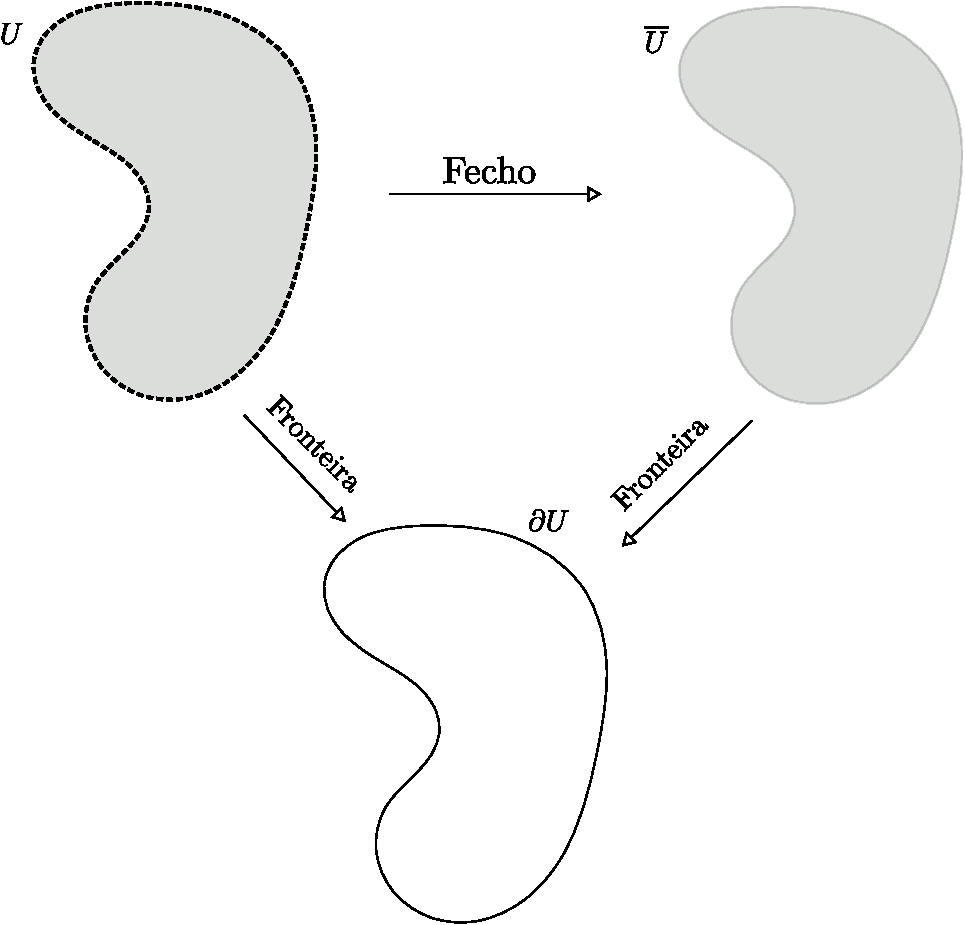
\includegraphics[width=0.7\linewidth]{Figuras/fecho-fronteira}
\caption{A esquerda um subconjunto $U$ do plano complexo. A direita o fecho e em baixo a fronteira de $U$.
Esta figura também destaca que $\partial U = \partial \overline{U}$.}
\label{fig:fecho-fronteira}
\end{figure}


\medskip 
Um subconjunto $B\subset \mathbb{C}$ é chamado de {\bf conjunto limitado}\index{Conjunto!limitado} 
se existe algum número real (finito) $r>0$ tal que 
$B\subset D(0,r)$, isto é, $B$ é limitado se ele está inteiramente contido em um disco de raio
$r>0$. Alternativamente, $B$ é limitado se existe $r>0$ tal que 
para todo $z\in B$ temos que  $|z|<r$. Se $B\subset \mathbb{C}$ é um conjunto limitado,
então definimo o {\bf diâmetro} de $B$ como sendo o número real 
\[
\mathrm{diam}(B) \equiv \sup_{z,w\in B}|z-w|,
\] 
onde ``$\sup$'' denota o supremo do conjunto de todas as distâncias $|z-w|$ com $z$ e $w$
variando por todo conjunto $B$. A única propriedade que vamos precisar nesta seção sobre
supremo é que se $z$ e $w$ são dois pontos arbitrários em $B$ então a seguinte desigualdade é satisfeita
\[
|z-w|\leqslant \mathrm{diam}(B).
\]
%Veja o Apêndice \ref{Apend-sup-inf}, para maiores detalhes
%sobre a definição precisa e propriedades básicas de supremos.


\medskip

Finalmente estamos prontos para apresentar uma das noções mais importantes desta seção
que é a noção de compacidade. Dizemos que um subconjunto $K\subset \mathbb{C}$ é um 
{\bf conjunto compacto}\index{Conjunto!compacto} se $K$ é ao mesmo tempo um conjunto 
fechado e limitado. 

Existe uma caracterização, muito importante, dos compactos de $\mathbb{C}$ 
em termos de sequências. Para enunciarmos este resultado precisamos antes da definição 
do que é uma subsequência.\index{Subsequência}

Uma {\bf subsequência}\index{Subsequência} de uma 
sequência $(z_n)_{n\in\mathbb{N}}\equiv \{z_1,z_2,z_3,\ldots\}$ de números complexo 
é simplesmente uma sequência $(z_{n_k})_{k\in\mathbb{N}}$ construída selecionando-se da sequência original
somente os elementos de índice $1\leqslant n_1<n_2<n_3<\ldots$, onde $(n_k)_{k\in\mathbb{N}}$ pode ser escolhida como 
sendo qualquer sequência infinita estritamente crescente de números naturais.

Por exemplo, $\{z_{4},z_{7},z_{39},z_{100},\ldots\}$ é um exemplo de uma subsequência da 
sequência $\{z_1,z_2,z_3,z_4,\ldots\}$. Neste exemplo $n_1=4, n_2=7, n_3=39, n_4=100$ e assim por diante.
Em geral, qualquer função estritamente crescente $f:\mathbb{N}\to\mathbb{N}$ 
determina uma subsequência e vice-versa. Mais precisamente, dada uma sequência 
$(z_n)_{n\in\mathbb{N}}\equiv\{z_1,z_2,z_3,\ldots\}$ a subsequência determinada por $f$ é 
definida como sendo a sequência $\{z_{f(1)},z_{f(2)},z_{f(3)},\ldots\}$. 
Esta subsequência é denotada por $(z_{f(n)})_{n\in\mathbb{N}}$. Apesar de ser bastante
clara e sugestiva, esta notação é menos usada que a notação anterior $(z_{n_k})_{k\in\mathbb{N}}$.
Mas elas podem ser encaradas do mesmo ponto de vista pensando que $n_k=f(k)$, para todo $k\in\mathbb{N}$,
para alguma função $f:\mathbb{N}\to\mathbb{N}$ estritamente crescente. 
Um fato importante de se observar é que, vista como um conjunto, uma subsequência deve ser sempre 
um subconjunto da sequência original, isto é, $(z_{n_k})_{k\in\mathbb{N}}\equiv \{z_{n_1},z_{n_2},\ldots\}
\subset \{z_1,z_2,\ldots\}\equiv (z_n)_{n\in\mathbb{N}}$. Uma grande vantagem da notação 
$(z_{n_k})_{k\in\mathbb{N}}$ é que 
se quisermos considerar uma subsequência desta subsequência, 
basta modificar a notação acrescentando mais um subíndice ficando, por exemplo, 
com $(z_{n_{k_{p}}})_{p\in\mathbb{N}}$, onde fica subentendido que $k_1<k_2<k_3\ldots$ e  
$\{n_{k_1},n_{k_2},\ldots\}\subset \{n_1,n_2,\ldots\}$.


\begin{teorema}
Um conjunto $K\subset \mathbb{C}$ é compacto se, e somente se, toda sequência $(z_n)_{n\in\mathbb{N}}$
contida em $K$, possui alguma subsequência que converge para algum ponto pertencente a $K$.
\end{teorema}

% \begin{proof}
% Vamos mostrar primeiro que se $K$ é compacto então qualquer sequência $(z_n)_{n\in\mathbb{N}}$
% contida em $K$, possui alguma subsequência convergente.
% Para isto vamos considerar as seguintes duas sequências de números reais associadas à $(z_n)_{n\in\mathbb{R}}$ dadas por
% \begin{align*}
% x_n \equiv \Re(z_n) \qquad\text{e}\qquad y_n\equiv \Im(z_n).
% \end{align*}
% Já que estamos assumindo que $K$ é compacto e $(z_n)_{n\in\mathbb{N}}$
% está contida em $K$, então $K$ é limitado. Assim existe 
% $r>0$ tal que $|z_n|<r$. Aplicando o Lema \ref{lema-re-im-modulo} 
% concluímos que $|x_n|< r$ e $|y_n|< r$, para todo $n\in\mathbb{N}$. 
% Agora usamos o fato que toda sequência de números reais limitada, possui
% uma subsequência convergente. Logo existe uma subsequência $(x_{n_k})_{k\in\mathbb{N}}$ 
% tal que $x_{n_k}\to x$ quando $k\to\infty$. Agora olhamos para a 
% subsequência $(y_{n_k})_{k\in\mathbb{N}}$. Já que ela é uma subsequência de $(y_n)_{n\in\mathbb{N}}$ então 
% ela é limita. Portanto podemos garantir que ela possui 
% uma subsequência $(y_{n_{k_p}})_{p\in\mathbb{N}}$ tal que $y_{n_{k_p}}\to y$, quando $p\to\infty$.  
% Note que $x_{n_{k_p}}\to x$, quando $p\to\infty$ uma vez que qualquer subsequência de uma sequência 
% convergente também é convergente e o limite é o mesmo. 
% Para finalizar esta parte da prova vamos mostrar que $(z_{n_{k_p}})_{p\in\mathbb{N}}$ converge
% para $z=x+iy$, quando $p\to\infty$. De fato, pela desigualdade triangular temos que 
% \begin{align*}
% \lim_{k\to\infty} |z_{n_{k_p}} -z |
% &=
% \lim_{k\to\infty} |\Re(z_{n_{k_p}})+i\Im(z_{n_{k_p}}) - (x+iy)|
% \\
% &=
% \lim_{k\to\infty} |x_{n_{k_p}}+iy_{n_{k_p}} - (x+iy)|
% \\
% &=
% \lim_{k\to\infty} |x_{n_{k_p}}+iy_{n_{k_p}} - (x+iy)|
% \\
% &=
% \lim_{k\to\infty} |(x_{n_{k_p}}-x)+i (y_{n_{k_p}}-y)|
% \\
% &\leqslant 
% \lim_{k\to\infty} |(x_{n_{k_p}}-x)|
% +
% \lim_{k\to\infty} |(y_{n_{k_p}}-y)|=0.
% \end{align*}

% Vamos mostrar agora que se $K$ tem a propriedade de que qualquer sequência em $K$ possui 
% subsequência que converge para um ponto em $K$, então $K$ é limitado e fechado. 


% Suponha por absurdo que $K$ não é limitado.
% Então para cada $n\in\mathbb{N}$ existe $z_n\in K$ tal que $n<|z_n|$. Logo qualquer subsequência
% $(z_{n_k})_{k\in\mathbb{N}}$ satisfaz $n_k<|z_{n_k}|$ e portanto não converge o que é um absurdo.


% Resta mostrar que $K$ é fechado. Pela Proposição \ref{prop-caract-fechados-sequencias} 
% sabemos que isto é equivalente a mostrar que $K$ possui todos seus pontos de acumulação,
% isto é, $K=\overline{K}$. 
% Seja $z\in \overline{K}$. Então pela definição do fecho de $K$, podemos afirmar que 
% existe uma sequência $(z_n)_{n\in\mathbb{N}}$ tal que $z_n\in K$ para todo $n\in\mathbb{N}$ 
% e além do mais $z_n\to z$. Já que a sequência $(z_n)_{n\in\mathbb{N}}$ é convergente, qualquer
% de suas subsequências também convergem e para o mesmo limite, que no caso é $z$.
% Da propriedade do nosso conjunto $K$ existe pelo menos uma subsequência 
% $(z_{n_{k}})_{k\in\mathbb{N}}$
% que converge para um ponto de $K$, mas como acabamos de mencionar o limite desta subsequência é 
% exatamente $z$ e portanto pela nossa hipótese, este deve ser um ponto de $K$. O que mostra que 
% todo ponto de $\overline{K}$ é também um ponto de $K$, isto é, $\overline{K}\subset K$.
% Mas por outro lado, sabemos que a inclusão reversa $K\subset \overline{K}$ é sempre válida para qualquer 
% conjunto. Logo $K=\overline{K}$ e portanto $K$ é fechado e isto encerra a prova do teorema.
% \end{proof}



Outra propriedade importante sobre conjuntos compactos, que é usada na prova do importante
Teorema de Cauchy-Goursat, é enunciada no teorema abaixo. 

\begin{teorema}[Teorema de Cantor]
Para cada $n\in\mathbb{N}$ seja $K_n\subset \mathbb{C}$ um conjunto compacto não-vazio. Suponha que $K_{n}\supset K_{n+1}$ e $\mathrm{diam}(K_n)\to 0$, quando $n\to\infty$. Então existe um único ponto $z\in\mathbb{C}$ tal que $z\in K_n$ para todo $n\in\mathbb{N}$, ou seja, 
\[
z\in \bigcap_{n=1}^{\infty} K_n.
\]


\end{teorema}

\begin{proof}
Já que para cada $n\in\mathbb{N}$ estamos assumindo que $K_n$ é não-vazio, então existe algum
$z_n\in K_n$. Como $\mathrm{diam}(K_n)\to 0$ temos que a sequência $(z_n)_{n\in\mathbb{N}}$
é uma sequência de Cauchy. 

\begin{figure}[h]
\centering
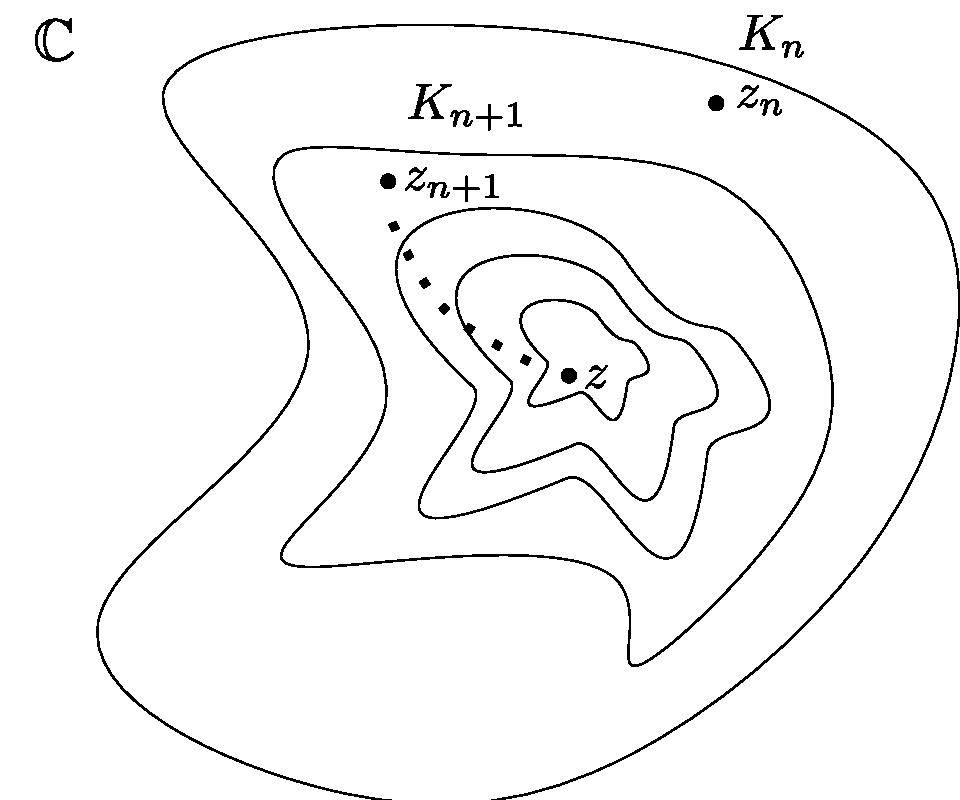
\includegraphics[scale=0.6]{Figuras/teorema-cantor}
\caption{A construção da sequência $(z_n)_{n\in\mathbb{N}}$.}
\label{fig:teorema-cantor}
\end{figure}


De fato, já que $\mathrm{diam}(K_n)\to 0$ sabemos que para qualquer $\varepsilon>0$ vai existir existe $N_0\in\mathbb{N}$ tal que se $n\geqslant N_0$ então 
$\mathrm{diam}(K_n)<\varepsilon$. Por hipótese, 
para qualquer $j\geqslant N_{0}$ temos $K_{N_0}\supset K_{j}$
e portanto os pontos $z_n$ e $z_{m}$ pertencem a $K_{N_0}$. 
Desta observação e da definição de supremo segue
que $|z_n-z_m|\leq \mathrm{diam}(K_n)<\varepsilon$
para todo $m,n\geqslant N_0$ mostrando assim que $(z_n)_{n\in\mathbb{N}}$
é uma sequência de Cauchy. Como $\mathbb{C}$ é completo. Sabemos que existe $z\in\mathbb{C}$
tal que $z_n\to z$, quando $n\to\infty$. Como para cada $n\in\mathbb{N}$ temos que $K_n$ é compacto e $\{z_n,z_{n+1},\ldots\}$
é uma sequência em $K_n$. Então $z=\lim_{n\to\infty} z_n$ também pertence a $K_n$.
Portanto $\cap_{n=1}^{\infty}K_n$ é não-vazio. Para mostrar que $z$ é o único ponto 
que pertence a esta interseção infinita argumentamos por absurdo. Suponha que exista $z'\in \cap_{n=1}^{\infty}K_n$ com $z'\neq z$. Então $|z'-z|>0$. Por outro lado, como $z,z'\in K_n$ 
para todo $n\in\mathbb{N}$ logo
\[
0<|z-z'|\leqslant \mathrm{diam}(K_n), \qquad \forall n\in\mathbb{N}
\]
o que é um absurdo já que $\lim_{n\to\infty}\mathrm{diam}(K_n)=0$.
\end{proof}

\subsection{Conjuntos Conexos e Domínios}
\label{subsec-coonj-conexos-dominios}

A última noção de topologia que vamos precisar é a de conexidade. 
Um conjunto $B\subset \mathbb{C}$ é dito {\bf conexo}\index{Conjunto!conexo} 
se não é possível encontrar dois subconjuntos do plano complexo $U$ e $V$ abertos, 
disjuntos ($U\cap V = \emptyset)$, não-vazios e tais que: 
\begin{itemize}
	\item $B\cap U\neq \emptyset$;  
	\item $B\cap V\neq \emptyset$; e
	\item $B\subset V\cup U$.
\end{itemize}

\begin{figure}[h]
\centering
\includegraphics[width=0.9\linewidth]{"Figuras/fig-conjuntos-conexos"}
\caption[Conjunto Conexo]{Exemplo de um conjunto $B$ conexo. No lado esquerdo da figura temos um exemplo de um conjunto conexo $B$. 
No lado direito, podemos ver que o $B$ não pode ser separado 
por abertos $U$ e $V$ não-vazios, disjuntos, ambos interceptando $B$, e que cobrem $B$ ($B\subset U\cup V$).
Informalmente, vemos que $B$ não pode ser separado em dois pedaços (em que cada pedaço é um 
conjunto aberto). }
\label{fig:conjuntos-conexos}
\end{figure}


Esta definição de conexidade, formaliza, em um grande número de casos, a ideia do que seria 
um subconjunto do plano complexo formado por apenas um ``pedaço''. 
Excetuando alguns casos patológicos como, por exemplo, 
o do conjunto mostrado na Figura \ref{fig-pente}, podemos pensar em um 
conjunto conexo como sendo realmente um conjunto formado por um único ``pedaço''. 
Este é o caso quando o conjunto em questão é um \textit{domínio}.  


Na figura abaixo temos um exemplo simples de um conjunto $B$ que não é conexo.
Às vezes, nos referimos a tais conjuntos como desconexos. 


\begin{figure}[h]
\centering
\includegraphics[width=0.9\linewidth]{"Figuras/fig-conjunto-desconexo"}
\caption[Conjunto Conexo]{Exemplo de um conjunto $B$ que é desconexo. 
O conjunto $B$, formado pela união dos pontos pertencentes às duas regiões pintadas na
cor cinza escuro, no lado esquerdo da figura acima, é um exemplo de um conjunto que não é conexo. 
A direita mostramos como é possível separar $B$ 
por abertos $U$ e $V$ disjuntos não-vazios que: ambos interceptam $B$; e o cobrem.}
\label{fig:conjunto-desconexo}
\end{figure}


Um subconjunto $U\subset\mathbb{C}$ que é ao mesmo tempo aberto e conexo, 
será chamado de 
{\bf domínio}\index{Domínio}. Na próxima seção vamos mostrar que 
um domínio $U\subset \mathbb{C}$ por ser caracterizado pelos
caminhos existente nele. 



\section{Caminhos no Plano Complexo}

\begin{definicao}[Caminho Suave]\label{def-caminho-em-C}
Seja $I=[a,b]\subset\mathbb{R}$ um intervalo não degenerado, isto é, $a<b$. 
Um caminho suave\index{Caminho!suave} 
em $\mathbb{C}$ é uma aplicação $\gamma:I\to \mathbb{C}$
possuindo derivada contínua em todos os pontos de $I$.
\end{definicao}

Antes de prosseguir devemos fazer algumas observações sobre a definição acima.
Primeira observação é que a condição de diferenciabilidade imposta nesta definição, 
deve ser entendida da seguinte forma.
Para cada $t\in I$ lembre-se que podemos escrever $\gamma(t) = \Re(\gamma(t))+i\Im(\gamma(t))$.
As funções $t\longmapsto \Re(\gamma(t))$ e $t\longmapsto \Im(\gamma(t))$ definem
duas funções reais chamadas de coordenadas do caminho $\gamma$.
Por simplicidade, vamos denotá-las por $x(t)\equiv\Re(\gamma(t))$ e 
$y(t)\equiv\Im(\gamma(t))$. 
Finalmente, a condição de suavidade
é que as funções coordenadas sejam deriváveis e que suas derivadas 
$t\longmapsto x'(t)$ e $t\longmapsto y'(t)$ sejam funções contínuas para todo $a<t<b$ e 
nos pontos $t=a$ e $t=b$ exigimos que os seguintes limites laterais existam e satisfaçam as seguintes
igualdades:
\[
\lim_{t\to a^{+}}x'(t) = x'(a)\equiv\lim_{h\to 0^{+}}\frac{x(a+h)-x(a)}{h}  
\]
e
\[
\lim_{t\to a^{+}}y'(t) = x'(b)\equiv \lim_{h\to 0^{-}}\frac{x(b+h)-x(b)}{h}  
\]

É claro que poderíamos também enunciar a condição de suavidade diretamente para $\gamma$
sem ter que apelar para suas funções coordenadas. Para isto tomaríamos, para cada $t$ no intervalo aberto $(a,b)$
\[
\gamma'(t) = \lim_{h\to 0} \frac{\gamma(t+h)-\gamma(t)}{h}
\]
e similarmente, 
\[
\gamma'(a) = \lim_{h\to 0^{+}} \frac{\gamma(a+h)-\gamma(a)}{h}
\qquad \text{e}\qquad 
\gamma'(b) = \lim_{h\to 0^{-}} \frac{\gamma(b+h)-\gamma(b)}{h}.
\]
Em seguida, exigiríamos que $\gamma'(t)$ variasse continuamente em $[a,b]$.
Esta definição seria mais elegante, mas para torná-la completamente precisa seria necessário antes
atentarmos para um detalhe, ainda não falamos o que é continuidade de funções 
a valores em $\mathbb{C}$. Muito provavelmente 
o leitor já deva estar imaginando que isto será feito com a base na definição de continuidade
de funções tomando valores em $\mathbb{R}^2$, já que na seção passada todos os conceitos topológicos
em $\mathbb{C}$ foram construídos em analogia aos de $\mathbb{R}^2$. 

Considerando então o caminho $\gamma$, como uma função tomando valores em $\mathbb{R}^2$
temos para cada $a<t<b$ a seguinte igualdade 
\begin{align*}
\gamma'(t) 
&= 
\lim_{h\to 0} \frac{\gamma(t+h)-\gamma(t)}{h}
=
\lim_{h\to 0} \frac{1}{h}\big(x(t+h),y(t+h)\big) - \big(x(t),y(t)\big)
\\[0.3cm]
&=
\lim_{h\to 0} \left( \frac{x(t+h)-x(t)}{h},\frac{y(t+h)-y(t)}{h} \right)
\\[0.3cm]
&=
(x'(t),y'(t)).
\end{align*}
Voltando para o plano complexo temos
\[
\gamma'(t) = x'(t)+iy'(t).
\]
De maneira análoga, estendemos a igualdade para os pontos $t=a$ e $t=b$.


\bigskip 

Se $\gamma:I\to\mathbb{C}$ é um caminho suave em $\mathbb{C}$ o ponto
$\gamma(a)$ é chamado de {\bf ponto inicial}\index{Ponto!inicial} 
e $\gamma(b)$ {\bf ponto terminal}\index{Ponto!terminal} do 
caminho $\gamma$. O conjunto imagem do caminho $\gamma$, isto é, 
o conjunto $\gamma(I)\subset\mathbb{C}$ é chamado de {\bf curva} no plano complexo
determinada por $\gamma$.
Em muitas situações abusamos da notação e chamamos a curva determinada por $\gamma$
de caminho $\gamma$. 
Quando $\gamma(a)=\gamma(b)$ dizemos que $\gamma$ é um 
{\bf caminho fechado}\index{Caminho!fechado} ou alternativamente que $\gamma$ é
um curva fechada.

\begin{exemplo}\label{exemplo-param-segreta}
O segmento de reta em $\mathbb{C}$ unindo os pontos quaisquer fixados 
$z_1=x_1+iy_1$ e $z_2=x_2+iy_2$
pode ser visto como um caminho suave representado pela função $\gamma:[0,1]\to\mathbb{C}$
dada por 
\[
\gamma(t) = z_1+t(z_2-z_1) = \big((1-t)x_1+tx_2\big)+i\big((1-t)y_1+ty_2\big).
\] 
\end{exemplo}

\begin{exemplo}\label{exemplo-param-circ}
A fronteira de um disco de centro $z=x+iy$ e raio $r>0$, isto é, $\partial D(z,r)$ 
pode ser vista como a imagem do caminho $\gamma:[0,2\pi]\to\mathbb{C}$ dado por
\[
\gamma(\theta) = z+r(\cos\theta+i\sen\theta) = (x+r\cos\theta)+i(y+r\sen\theta).
\]
\end{exemplo}

Da maneira como introduzimos o conceito de um caminho $\gamma:[a,b]\to\mathbb{C}$, 
temos automaticamente uma maneira de definir sua orientação. 
Intuitivamente, a orientação é dada pelo percurso 
do caminho a medida que o parâmetro $t$ cresce de $a$ para $b$. 
Assim dizemos que o caminho $\gamma$ está orientado do ponto 
inicial $\gamma(a)$ para o ponto terminal $\gamma(b)$. 

Definimos também o caminho reverso\index{Caminho!reverso} do $\gamma:[a,b]\to\mathbb{C}$
pela aplicação $\gamma^{-}:[a,b]\to\mathbb{C}$ dada por 
\begin{align}\label{formula-caminho-reverso}
\gamma^{-}(t) \equiv \gamma(a+b-t), \quad \text{para todo}\ t\in[a,b].
\end{align}
Note que as curvas $\gamma([a,b])$ e $\gamma^{-}([a,b])$ associadas à ambos $\gamma$ e seu reverso, 
são exatamente as mesmas, mas do ponto de vista de caminhos temos que o ponto inicial de um é o ponto 
terminal do outro e vice-versa. 


\begin{figure}[h]
\centering
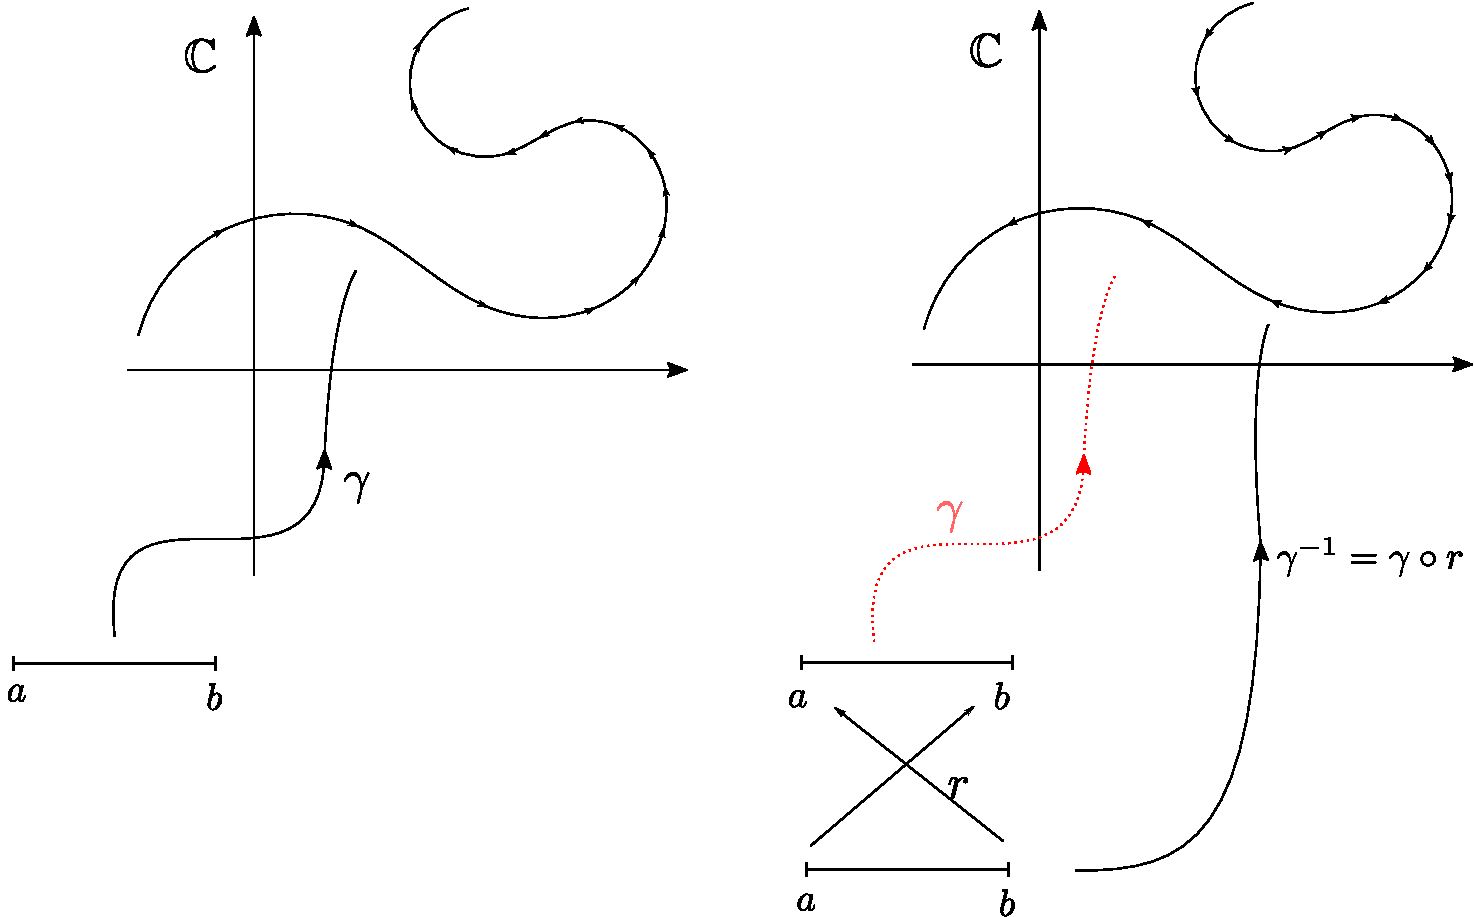
\includegraphics[width=0.9\linewidth]{Figuras/fig-gamma-gamma-reverso}
\caption{Um caminho suave $\gamma:[a,b]\to\mathbb{C}$ e seu reverso $\gamma^{-1}= \gamma\circ r$, onde $r(t)=a+b-t$.
Note que $r$ envia $a$ em $b$ e vice-versa, revertendo assim a orientação do intervalo $[a,b]$ e 
consequentemente o caminho $\gamma$.}
\label{fig-gamma-gamma-reverso}
\end{figure}



Exemplificamos agora como obter os caminhos reversos dos caminhos definidos no exemplos dados
acima.
No Exemplo \ref{exemplo-param-segreta} temos $\gamma(t) = z_1+t(z_2-z_1),\ t\in[0,1]$. Para obter a
expressão de $\gamma^{-1}$ basta aplicar a fórmula \eqref{formula-caminho-reverso} com $a=0$ e $b=1$
obtendo assim $\gamma^{-1}(t) = z_1+(1-t)(z_2-z_1)$. 
No caso do caminho do Exemplo \ref{exemplo-param-circ} temos 
$\gamma(\theta) = z+r(\cos\theta+i\sen\theta),\ t\in[0,2\pi]$. Agora aplicamos a fórmula 
\eqref{formula-caminho-reverso} com $a=0$ e $b=2\pi$ obtendo portanto 
$\gamma^{-1}(\theta) = z+r(\cos(2\pi-\theta)+i\sen(2\pi-\theta)),\ t\in[0,2\pi]$.

\begin{definicao}[Caminho suave por partes]
\label{def-caminho-suave-partes}
\index{Caminho!suave por partes}
Um caminho suave por partes em $\mathbb{C}$ é uma coleção finita de caminhos suaves
$\gamma_{1}:[a_1,b_1]\to\mathbb{C}$, $\gamma_{2}:[a_2,b_2]\to\mathbb{C}$, \ldots, 
$\gamma_{n}:[a_n,b_n]\to\mathbb{C}$, satisfazendo para cada $1\leqslant i\leqslant n-1$
as seguintes relações $\gamma_{i}(b_i)=\gamma_{i+1}(a_{i+1})$.
\end{definicao}


Será conveniente usar a notação $\gamma_1*\gamma_2*\ldots*\gamma_n$ para denotar um caminho suave
por partes $\gamma$ como na definição acima. Analogamente, tal caminho suave por partes é dito
fechado se $\gamma_1(a_1)=\gamma_{n}(b_n)$. Como no caso de caminhos suaves, 
o ponto $\gamma_1(a_1)$ é chamado de ponto inicial e o ponto 
$\gamma_n(b_n)$ é chamado de ponto terminal. 


Por exemplo, podemos ver um polígono de 6 lados cujos vértices são os 
pontos $z_1,z_2,\ldots, z_6\in\mathbb{C}$ mostrados na Figura \ref{fig-polig-6-lados}
como um caminho $\gamma = \gamma_1*\gamma_2*\ldots*\gamma_6$.

\begin{figure}[h]
\centering
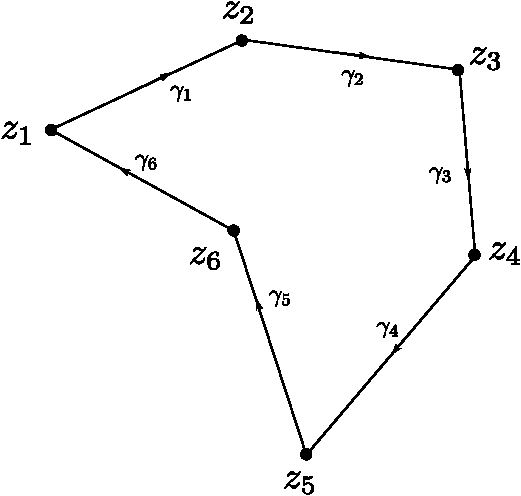
\includegraphics[scale=0.6]{Figuras/fig-polig-6-lados}
\caption{O polígono determinado pelo caminho suave por partes $\gamma= \gamma_1*\ldots*\gamma_6$}
\label{fig-polig-6-lados}
\end{figure}


onde para cada $1\leqslant i\leqslant 6$ temos 
\begin{align*}
\gamma_1(t) = z_1+t(z_2-z_1), \quad t\in [0,1];\\
\gamma_2(t) = z_2+t(z_3-z_2), \quad t\in [0,1];\\
\vdots\qquad \qquad\qquad \qquad \\
\gamma_6(t) = z_6+t(z_1-z_6), \quad t\in[0,1].
\end{align*}

\bigskip 





Em muitas situações é mais conveniente ter os caminhos $\gamma_i$'s de 
$\gamma=\gamma_1*\gamma_2*\ldots*\gamma_n$
parametrizados de forma que seus domínios sejam intervalos ``consecutivos'', isto é, seus pontos
de bordo satisfazem 
\[
a_1<b_1=a_2<b_2=a_3<\ldots<b_{n-1}=a_{n}<b_n.
\]
Mais conveniente ainda é poder trabalhar com caminhos cujos intervalos de definição 
formem uma coleção consecutiva de $n$ subintervalos do intervalo $[0,1]$. 

Dado um caminho suave por partes $\gamma= \gamma_1*\gamma_2*\ldots*\gamma_n$
podemos associar a ele um novo caminho suave por partes 
que será chamado de {\bf normalizado}\index{Caminho!normalizado}.
Para fazer isto, primeiro dividimos o intervalo $[0,1]$ em $n$ subintervalos de
mesmo comprimento
\[
\left[0,\frac{1}{n} \right],
\left[\frac{1}{n},\frac{2}{n} \right],
\ldots
\left[\frac{n-1}{n},1 \right].
\]
Em seguida, para cada $1\leqslant j\leqslant n$, vamos definir uma aplicação bijetiva (afim) 
$r_{j}:[j-1/n,j/n]\to [a_j,b_j]$ que mapeia o subintervalo $[j-1/n,j/n]$ no intervalo $[a_j,b_j]$. 
Esta bijeção é dada por 
\[
r_j(t) = n(b_j-a_j)t-j(b_j-a_j)+b_j, \quad t\in\left[\frac{j-1}{n},\frac{j}{n}\right].
\]
Estas aplicações $r_j$'s são muitas vezes chamadas de re-parametrizações. 
Agora consideramos os caminhos $\gamma_{j}\circ r_j$ com $1\leqslant j\leqslant n$.
Então é fácil ver que $\gamma_{j}\circ r_j$ é um caminho suave em $\mathbb{C}$ e além do 
mais o ponto final de $\gamma_{j-1}\circ r_{j-1}$ coincide com o ponto inicial de 
$\gamma_{j}\circ r_j$. Desta maneira o caminho $\gamma$ pode ser visto como definido 
no intervalo $[0,1]$. 

Dizemos que um caminho suave por partes (normalizado como acima) 
é {\bf simples}\index{Caminho!simples}, se aplicação $\gamma:[0,1]\to\mathbb{C}$ que o define
é injetiva, exceto possivelmente pelos pontos $t=0$ e $t=1$. Mais precisamente, $\gamma(s)\neq \gamma(t)$
para $0\leqslant s<t<1$ e é permitido $\gamma(0)=\gamma(1)$. 
Do ponto de vista geométrico, um caminho simples representa uma curva no plano sem 
auto-interseção, exceto possivelmente pelos pontos inicial e terminal. 


Já temos todos terreno preparado para introduzir uma classe de curvas 
que serão de enorme importância no estudo de integração no plano 
complexo. 

\begin{definicao}
[Curva de Jordan]
\label{def-curva-jordan}
\index{Curva!de Jordan}
Uma curva de Jordan suave por partes é a imagem de um caminho suave por partes, fechado e simples. 
\end{definicao}


\begin{figure}[h]
\centering
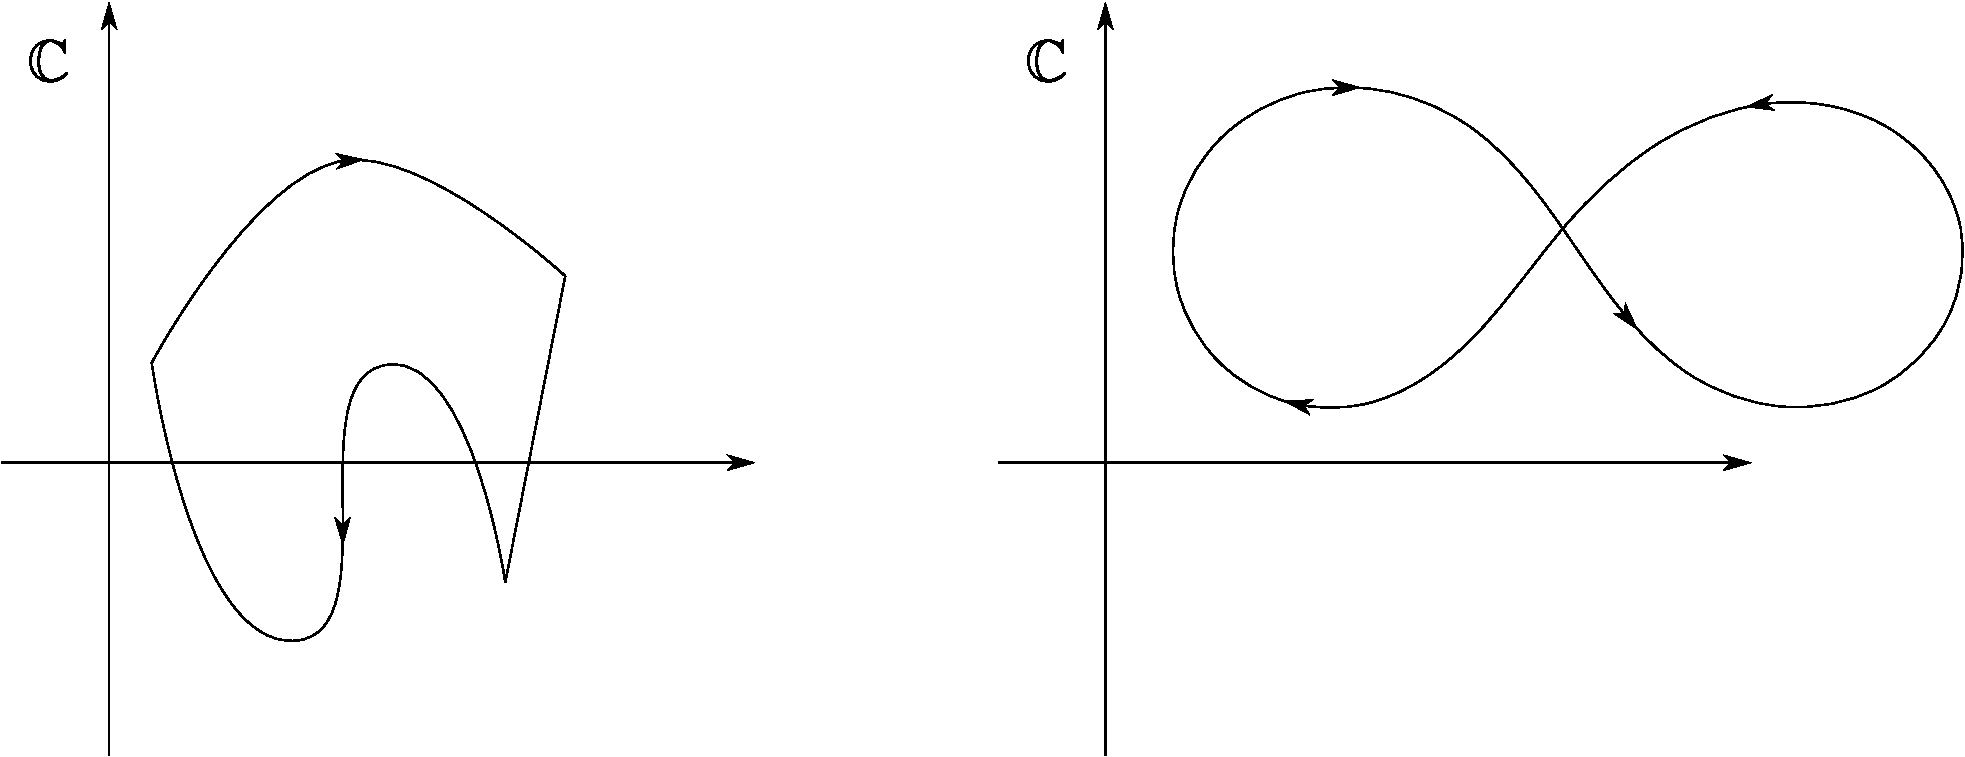
\includegraphics[scale=0.4]{Figuras/fig-curvas-fechadas}
\caption{Caminhos fechados suaves por partes. O caminho da esquerda está associado a uma curva de Jordan. A curva a direita não é uma curva de Jordan pois ela possui um ponto de auto-interseção.}
\label{fig-curvas-fechadas}
\end{figure}



Um dos resultados mais importantes sobre curvas de Jordan é um teorema devido a Jordan.
Ele afirma que uma curva de Jordan suave por partes $\gamma$ divide o plano $\mathbb{R}^2$
em exatamente dois abertos disjuntos, um deles limitado e o outro ilimitado, sendo 
$\gamma$ a fronteira comum entre estes dois abertos. Esse resultado, embora de fácil 
intuição é de demostração bastante elaborada. Atualmente existem vários textos que provam
este teorema. O leitor interessado pode encontrar uma prova deste teorema um pouco 
mais moderna e bem detalhada no Apêndice B da referência \cite{MR1976398}.


\begin{definicao}
\label{def-comp-caminho}
\index{Comprimento!de um caminho}
O comprimento de um caminho suave $\gamma:[a,b]\to\mathbb{C}$ é definido como sendo o número real
\[
\ell(\gamma)\equiv 
\int_{a}^{b} |\gamma'(t)|\, dt.
\]
Se $\gamma$ é um caminho suave por partes da forma $\gamma=\gamma_1*\gamma_2*\ldots*\gamma_n$
então definimos o comprimento de $\gamma$ como sendo $\ell(\gamma)\equiv \ell(\gamma_1)+\ldots+\ell(\gamma_n)$.
\end{definicao}


\begin{exemplo}
Se $\gamma:[0,2\pi]\to\mathbb{C}$ é o caminho dado por $\gamma(\theta)=z+r(\cos\theta+i\sen\theta)$,
com $0\leqslant \theta\leqslant 2\pi$ temos que 
\[
\gamma'(\theta) = \frac{d}{d\theta}[z+r(\cos\theta+i\sen\theta)]=r(-\sen\theta+i\cos\theta).
\]
Portanto $|\gamma'(\theta)|=r$ e assim 
\[
\ell(\gamma) 
= 
\int_{0}^{2\pi} |\gamma'(\theta)|\, d\theta 
= 
r\int_{0}^{2\pi}\, d\theta 
=
2\pi r.
\]
\end{exemplo}

Pensando em um caminho $\gamma:[a,b]\to\mathbb{C}$ como uma função descrevendo a posição de uma partícula
no instante $t$ o número $\ell(\gamma)$ pode ser interpretado como a distância total percorrida pela 
partícula durante o intervalo de tempo $[a,b]$. Portanto se ela se percorre várias vezes certos
trechos da curva determinada por $\gamma$ o resultado da distância percorrida pode ser
maior que o comprimento da curva em si. Se no exemplo anterior substituímos o domínio de $\gamma$
pelo intervalo $[0,4\pi]$ vamos verificar que o novo comprimento deste caminho será duas vezes maior que
o comprimento encontrado no exemplo anterior. Isto se deve ao fato de que neste novo caminho percorremos
o círculo de centro $z$ e raio $r$ duas vezes.  


\bigskip 


\subsection{Conjuntos Conexos e Conexidade por Caminhos}

Introduzimos na Subseção \ref{subsec-coonj-conexos-dominios} 
o conceito de conexidade e de domínio no plano complexo. 
Vamos encerrar esta seção falando novamente sobre domínios 
e suas relações com o conceito de caminho, visto nesta seção.

\begin{definicao}[Conexidade por Caminhos]
\label{def-conexo-caminho}
\index{Conjunto!conexo por caminhos}
Um subconjunto $B\subset \mathbb{C}$ é dito conexo por caminhos se dados quaisquer 
$z,w\in B$ existe um caminho suave por partes $\gamma:[0,1]\to\mathbb{C}$ tal que 
$\gamma([0,1])\subset B$, $\gamma(0)=z$ e $\gamma(1)=w$.
\end{definicao}


\begin{proposicao}
Se $U\subset\mathbb{C}$ é um conjunto conexo por caminhos então $U$ é conexo.
\end{proposicao}
Apesar de ser bastante intuitiva a afirmação da proposição acima, sua prova pode ser um pouco
desafiante para o leitor menos experiente. Uma maneira de provar esta proposição é por absurdo.
Supomos que $U$ admite uma cisão não-trivial, isto é, existem abertos disjuntos $V_1,V_2$, não-vazios 
tais que $V_1\cup V_2 =U$. Já que ambos $V_1$ e $V_2$ são não-vazios podemos escolher $z\in V_1$ e $w\in V_2$.
Como estamos assumindo que $U$ é conexo por caminhos, 
então deve existir um caminho suave por partes 
$\gamma:[0,1]\to\mathbb{C}$ tal que $\gamma([0,1])\subset U$.
Próximo passo seria mostra que esta última inclusão implica que $V_1\cap V_2\neq \emptyset$
o que é absurdo. Esta parte é a parte mais elaborada deste argumento. 
Os detalhes serão apresentados em uma série de exercícios guiados no final desta seção. 


Devemos advertir que, em geral, a recíproca da proposição acima é falsa. 

\begin{figure}[h]
\centering
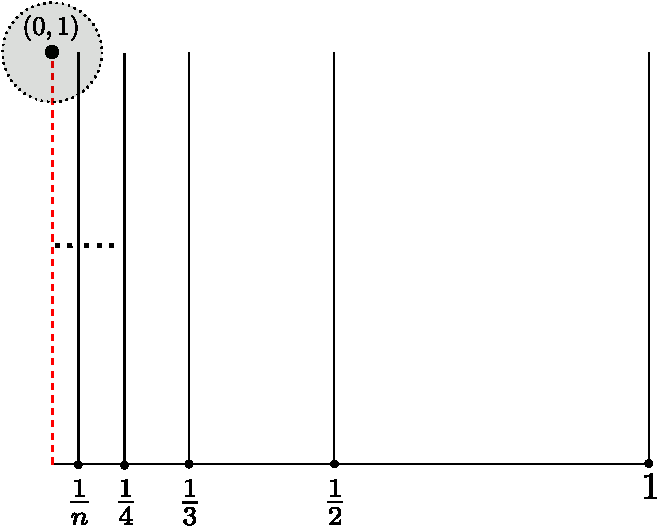
\includegraphics[scale=0.55]{Figuras/fig-pente}
\caption{O Pente Infinito}
\label{fig-pente}
\end{figure}

O ``pente infinito'' é um exemplo 
clássico de subconjunto conexo do plano que não é conexo por caminho.
O pente infinito é o subconjunto $\mathscr{P}$ do plano complexo, composto pelo ponto $(0,1)\in\mathbb{C}$
unido com os seguintes segmentos de reta: o segmento unindo o ponto $(0,0)$ ao ponto $(1,0)$ (base do pente);
e para cada $n\in\mathbb{N}$, o segmento unindo o ponto $(1/n,0)$ a $(1/n,1)$ (os ``dentes''do pente), 
veja a Figura \ref{fig-pente}.



A parte mais delicada de mostrar a conexidade do pente está relacionada 
a ideia intuitiva de que pente parece ter dois ``pedaços'': um contendo a ``base'' e os 
``dentes'' do pente; e outro contendo o ponto $(0,1)$. Isto porque não existe nenhum ``dente''
unindo o ponto $(0,0)$ da base do pente ao ponto $(0,1)$. 

Por outro lado, como sugere a figura acima, é impossível encontrar abertos disjuntos não-vazios
$U$ e $V$ tais que $\mathscr{P}\subset U\cup V$ e $(0,1)\in U$ e 
$\mathscr{P}\cap V\neq \emptyset$.
De fato, se existissem tais conjuntos existiria uma bola aberta centrada em $(0,1)$ 
com raio positivo, mas esta boa necessariamente interceptaria infinitos ``dentes'' 
evitando assim que o ponto $(0,1)$ e os demais pontos do pente possam ser separados
por abertos.

\medskip 

Vamos mostrar a seguir um resultado muito importante sobre a relação de conexidade e de 
conexidade por caminhos. Ele afirma que se $U\mathbb{C}$ é um 
conjunto aberto e conexo então 
quaisquer par de pontos em $U$ podem ser ligados por um caminho, suave por partes, inteiramente 
contido em $U$ e vice-versa. 

Alertamos o leitor menos experiente que a prova deste teorema pode ser omitida numa primeira
leitura e que as ideias envolvidas nela não são usadas no restante do texto.

\begin{teorema}\label{teo-conexo-conexo-caminhos}
Seja $U$ um subconjunto aberto  de $\mathbb{C}$. Então $U$ é conexo se, e somente se, 
$U$ é conexo por caminhos.
\end{teorema}

% \begin{proof}
% Vamos mostrar primeiro que se $U$ é um aberto conexo, então $U$ é conexo por caminhos. 
% De fato, primeiro para cada $z\in U$ seja $\mathscr{C}_{U}(z)$ o conjunto de todos os pontos
% $w\in U$ tais que $z$ e $w$ podem ser unidos por um caminho suave por partes inteiramente 
% contido em $U$, isto é, 
% \[
% \mathscr{C}_{U}(z) = 
% \left\{
% w\in U: 
% \begin{array}{l}
% \text{existe um caminho suave por partes}\ \gamma:[0,1]\to\mathbb{C}\\
% \text{tal que}\ \gamma([0,1])\subset U,\  \gamma(0)=z\ \text{e}\ \gamma(1)=w
% \end{array}
% \right\}.
% \] 
% Desta forma mostrar que $U$ é conexo por caminho se reduz a mostrar que 
% dado qualquer $z\in U$, então temos que $\mathscr{C}_{U}(z)=U$, uma vez que esta 
% igualdade significaria que se escolhemos qualquer ponto $w\in U$, então somos capazes 
% de encontrar um caminho, completamente contido em $U$, ligando $z$ a $w$. 

% Para mostrar que a igualdade acima é válida vamos mostrar primeiro que 
% para qualquer $z\in U$ dado que $\mathscr{C}_{U}(z)$ é um subconjunto aberto do plano complexo.
% Observe que independentemente da escolha de $z\in U$ o conjunto $\mathscr{C}_{U}(z)$ é não-vazio
% já que caminho constante liga $z$ a si mesmo. Continuando, para verificar 
% $\mathscr{C}_{U}(z)$ é aberto tomamos um ponto $w$ arbitrário em $\mathscr{C}_{U}(z)$.
% Como $\mathscr{C}_{U}(z)$ é sempre um subconjunto de $U$ então $w$ é um ponto de $U$, logo
% existe algum $r>0$ tal que $D(w,r)\subset U$. Vamos mostrar que todos os 
% pontos deste disco estão também contidos em $\mathscr{C}_{U}(z)$. 
% Feito isto podemos concluir que $w$ é um ponto interior de $\mathscr{C}_{U}(z)$. 
% Para mostrar isto basta observar que pela definição de 
% $\mathscr{C}_{U}(z)$ que existe algum caminho $\gamma_1:[0,1]\to\mathbb{C}$ totalmente contido em $U$
% unindo $z$ a $w$. Por outro lado, dado um ponto arbitrário $w' \in D(w,r)$ 
% temos que o caminho $\gamma_2:[1,2]\to\mathbb{C}$ dado por $\gamma_2(t)=w+(t-1)(w'-w)$,
% cuja curva associada é o segmento de reta unindo $w$ a $w'$ 
% é também um caminho totalmente contido em $D(w,r)\subset U$.
% Logo $\gamma_1*\gamma_2$ é um caminho suave por partes totalmente contido em $U$ unindo $z$ a $w'$.
% O que mostra que $w'\in \mathscr{C}_{U}(z)$. Como $w'$ foi escolhido arbitrariamente 
% em $D(w,r)$ temos que todo este disco está contido em $\mathscr{C}_{U}(z)$ o que implica que $w$
% é um ponto interior de $\mathscr{C}_{U}(z)$. Já que $w$ também foi escolhido arbitrariamente em 
% $\mathscr{C}_{U}(z)$ concluímos que este conjunto é aberto, pois todos seus pontos são pontos 
% interiores.

% Suponha, por absurdo, que 
% $V\equiv U\setminus \mathscr{C}_{U}(z)$ é um conjunto não-vazio.
% Seja $z'$ um ponto qualquer de $V$. Observe que $\mathscr{C}_{U}(z')$ 
% é disjunto de $\mathscr{C}_{U}(z)$, pois se existisse 
% um ponto $z''\in \mathscr{C}_{U}(z)\cap \mathscr{C}_{U}(z')$ 
% existiria um caminho $\gamma_1$ suave por partes totalmente contido em $U$ unindo
% $z$ a $z''$ e da mesma forma existiria um caminho $\gamma_2$ suave por partes 
% totalmente contido em $U$ unindo $z''$ a $z'$. Mas então $\gamma_1*\gamma_2$
% seria um caminho suave por partes totalmente contido em $U$ unindo $z$ a $z'$ 
% o que contraria a definição de $V$.
% Além de termos $\mathscr{C}_{U}(z)\cap \mathscr{C}_{U}(z')=\emptyset$ também temos que 
% \[
% V = \bigcup_{z'\in V} \mathscr{C}_{U}(z')
% \]
% é um conjunto aberto, já que ele é dado como uma união de conjuntos abertos. 
% Desta forma temos $U=\mathscr{C}_{U}(z)\cup V$ é uma união de dois abertos não-vazios 
% disjuntos o que é um absurdo, já que estamos assumindo que $U$ é conexo. 
% Esta contradição vem do fato de termos assumido 
% que $\mathscr{C}_{U}(z)\neq U$. Assim concluímos que todo aberto
% conexo de $\mathbb{C}$ é conexo por caminhos. 

% \medskip 
% Agora vamos provar a recíproca, isto é, se $U\subset \mathbb{C}$ é conexo 
% por caminhos então $U$ é conexo. 
% Para isto, seja $U$ um subconjunto de $\mathbb{C}$ conexo por caminhos.  
% Suponha, por absurdo, que $U=V_1\cup V_2$, onde $V_1$ e $V_2$ são 
% abertos não-vazios e disjuntos. Escolha arbitrariamente $z_1\in V_1$ e $z_2\in V_2$. 
% Por hipótese, existe algum caminho suave por partes $\gamma:[0,1]\to\mathbb{C}$ totalmente
% contido em $U$ unindo $z_1=\gamma(0)$ à $z_2=\gamma(1)$.
% Como $\gamma$ está totalmente contida em $U$ para todo $t\in [0,1]$ temos que
% $\gamma(t)\in V_1\cup V_2$. Já que $\gamma(0)=z_1$, $V_1$ e $V_2$ são abertos e $\gamma:[0,1]\to\mathbb{C}$
% é uma aplicação contínua então 
% o número 
% \[ 
% t^* \equiv \sup_{t\in [0,1]}\{ \gamma(t)\in V_1\}
% \]
% pertence ao intervalo aberto $(0,1)\subset\mathbb{R}$.
% Vamos mostrar a seguir que $\gamma(t^*)\in \partial V_2$.
% De fato, para qualquer $\varepsilon>0$ o disco $D(\gamma(t^*),\varepsilon)$
% intercepta $V_1$ e $V_1^c$ bem como $V_2$ e $V_2^c$. Para provar isto  usamos a continuidade de 
% $\gamma$ para verificar que para todo $\varepsilon>0$ existe $\delta>0$
% tal que se $|t-t^{*}|<\delta$ então $|\gamma(t)-\gamma(t^*)|<\varepsilon$. Em outras palavras
% para todo $t$ suficientemente próximo de $t^{*}$ temos $\gamma(t)\in D(\gamma(t^*),\varepsilon)$.
% Em seguida, observamos que pela definição de $t^*$ para qualquer $t$ fixado satisfazendo
% $t^{*}<t\leqslant 1$ temos $\gamma(t)\in V_2$. Se além desta condição impomos que 
% $|t-t^{*}|<\delta$ temos que este mesmo ponto $\gamma(t)\in D(\gamma(t^*),\varepsilon)$, pelas 
% escolhas de $\varepsilon$ e $\delta$. 
% Destas duas observações segue que a interseção $D(\gamma(t^*),\varepsilon)\cap V_2$
% é não-vazia. Por outro lado, como $t^{*}$ é o supremo dos $t$'s tais que $\gamma(t)\in V_1$
% sabemos que existe uma sequência $(t_n)_{n\in\mathbb{N}}$ tal que para todo $n\in\mathbb{N}$ 
% temos $0<t_n < t^*$, $t_n\to t^{*}$ e $\gamma(t_n)\in V_1$, para todo $n\in\mathbb{N}$.
% Pela definição de convergência de sequências existe $N_0\in\mathbb{N}$ tal que se $n\geqslant N_0$
% então $|t_n-t^{*}|<\delta$. Por esta última condição ser verdadeira segue que para qualquer $n\geqslant N_0$ temos
% $\gamma(t_n)\in D(\gamma(t^*),\varepsilon)$. Pela definição de $t_n$ temos que $\gamma(t_n)\in V_1$
% como $V_1$ e $V_2$ são disjuntos temos que $\gamma(t_n)\in V_2^c$ e portanto também é não vazia 
% a interseção $D(\gamma(t^*),\varepsilon)\cap V_2^c$. Destes argumentos podemos concluir que
% para todo $\varepsilon>0$ dado que 
% \[
% D(\gamma(t^*),\varepsilon)\cap V_2 \neq \emptyset 
% \qquad\text{e}\qquad
% D(\gamma(t^*),\varepsilon)\cap V_2^c \neq \emptyset.
% \]
% e finalmente que $\gamma(t^{*})\in \partial V_2$.
% Mas isto é um absurdo porque como $V_2$ é aberto sabemos que qualquer ponto de sua fronteira 
% está no seu complemento, mas como $\gamma$ está completamente contido em $U$ e também temos
% $U=V_1\cup V_2$ então segue que $\gamma(t^*)$ está necessariamente em $V_1$. Mas
% como $V_1$ é aberto existe algum $r>0$ tal que $D(\gamma(t^{*}),r)\subset V_1$.
% Tomando qualquer $\varepsilon>0$ tal que $\varepsilon<r$ concluiríamos que
% o disco $D(\gamma(t^{*}),\varepsilon)\subset D(\gamma(t^{*}),r)\subset V_1$
% mas como $D(\gamma(t^*),\varepsilon)\cap V_2 \neq \emptyset$ 
% então teríamos $V_1\cap V_2\neq\emptyset$ o que é um absurdo.

% \end{proof}


% \section{Limites e Continuidade de funções em $\mathbb{R}^2$}

% Nesta seção revisamos alguns conceitos básicos sobre limites e continuidade de funções 
% definidas em subconjuntos de $\mathbb{R}^2$ e tomando valores em $\mathbb{R}^2$. 
% Os conceitos topológicos considerados nesta seção são definidos de maneira
% análoga aos das seções anteriores usando a identificação natural
% de $\mathbb{C}$ com $\mathbb{R}^2$. 


% %Quando formos falar de distâncias nesta seção ao invés de usarmos a notação 
% %do módulo de $|z|$, onde $z=x+iy$ vamos usar a notação de norma do vetor $(x,y)$
% %isto é, $\|(x,y)\|=\sqrt{x^2+y^2}$, simplesmente para enfatizar que as ideias
% %discutidas não dependem da estrutura de produto de $\mathbb{C}$.


% Vamos nos restringir a aplicações definidas em conjuntos cujo o interior é não-vazio. 
% Para facilitar o leitor pode ter em mente conjuntos de $\mathbb{R}^2$ 
% correspondentes aos discos abertos de raio positivo ou 
% conjuntos como $D(z,r)\setminus\{z\}$ (o disco aberto de centro $z$ e raio $r$ exceto o ponto $z$).
% Como a estrutura de produto complexo não terá nenhuma relevância nesta seção vamos 
% conduzir as discussões usando a notação usual $(x,y)$ de vetores no plano. Já que esta
% seção tem caráter de revisão para
% manter semelhança com os textos de Cálculo em $\mathbb{R}^n$, vamos usar a linguagem 
% e notação de norma de vetor no lugar de falar do módulo de um número complexo. 

% O primeiro conceito que vamos recordar é o conceito de limite. 
% Seja $A\subset \mathbb{R}^2$ um conjunto de interior não-vazio. Vamos dizer que 
% um vetor $(a,b)\in\mathbb{R}^2$ é o limite de uma função 
% $f:A\subset \mathbb{R}^2\to\mathbb{R}^2$ quando $(x,y)\to (x_0,y_0)\in \overline{A}$
% se o vetor $f(x,y)$ fica arbitrariamente próximo do vetor $(a,b)$,  
% quando $(x,y)$ ficar arbitrariamente próximo de $(x_0,y_0)$. 
% Para denotar este fato usamos a notação 
% \[
% \lim_{(x,y)\to (x_0,y_0)} f(x,y) = (a,b).
% \]

% O problema com esta descrição intuitiva de limite  
% é que nela não temos um significa preciso do que é ``arbitrariamente próximo''. 
% Para remediar este problema vamos apresentar abaixo a definição formal de limite e 
% depois mostrar algumas outras formas equivalente dela.

% No que segue usamos a notação $\|\cdot\|$ para denotar a norma Euclidiana de um vetor
% em $\mathbb{R}^2$, isto é, 
% \[
% \|(x,y)\| = \sqrt{x^2+y^2}.
% \]



% \begin{definicao}\label{definicao-limite-R2}
% \index{Limite!de uma função}
% Seja $A\subset\mathbb{R}^2$ tal que interior de $A$ é não vazio e $f:A\to\mathbb{R}^2$ uma função.
% Dizemos que $f$ tem limite quando $(x,y)$ tende a $(x_0,y_0)\in \overline{A}$ (fecho de $A$) 
% se existe um vetor $(a,b)\in\mathbb{R}^2$ tal que para todo $\varepsilon>0$ dado existe um $\delta>0$
% tal que para todo ponto $(x,y)\in A$ satisfazendo $0<\|(x,y)-(x_0,y_0)\|<\delta$ 
% temos $\|f(x,y)-(a,b)\|<\varepsilon$. 
% Usamos a notação 
% \[
% \lim_{(x,y)\to (x_0,y_0)} f(x,y) = (a,b),
% \]
% para indicar que o ponto $(a,b)\in\mathbb{R}^2$ é o limite da função $f$ 
% quando $(x,y)$ tende a $(x_0,y_0)$. 
% \end{definicao}

% Uma observação importante a cerca desta definição é que não é necessário para falar de limite 
% que o ponto $(x_0,y_0)$ esteja no domínio da função $f$, isto é, não é necessário que a função $f$
% esteja definida no ponto $(x_0,y_0)$. Na verdade, basta que ela esteja definida em pontos suficientemente próximos
% deste ponto, o que de maneira mais precisa significa dizer que $(x_0,y_0)$ é um ponto do fecho do domínio de $f$
% que poderia não estar no domínio da função $f$. Este é inclusive um dos casos mais interessantes quando estamos 
% falando de limites. 


% Lembramos que cada função $f:A\subset\mathbb{R}^2\to\mathbb{R}^2$ é determinada por suas funções coordenadas, 
% isto é, existem funções reais $u:A\subset\mathbb{R}^2\to\mathbb{R}$ e 
% $v:A\subset\mathbb{R}^2\to\mathbb{R}$ tais que
% para todo $(x,y)\in A$ temos $f(x,y)=(u(x,y),v(x,y))$.
% Além do mais podemos verificar que existe o limite 
% \[
% \lim_{(x,y)\to (x_0,y_0)} f(x,y) = (a,b),
% \]
% se e somente se,
% \[
% \lim_{(x,y)\to (x_0,y_0)} u(x,y) = a
% \qquad \text{e} \qquad 
% \lim_{(x,y)\to (x_0,y_0)} v(x,y) = b,
% \]
% onde a definição destes limites acima são feitas de maneira análoga à 
% Definição \ref{definicao-limite-R2}, mas substituindo onde aparece $\|f(x,y)-(a,b)\|<\varepsilon$
% por $|u(x,y)-a|<\varepsilon$ e $|v(x,y)-b|<\varepsilon$, respectivamente. 


% Uma função $f$ pode ter limite quando $(x,y)$ tende a um ponto $(x_0,y_0)$, o ponto 
% $(x_0,y_0)$ pode ser um ponto do domínio de $f$, mas a imagem do ponto $(x_0,y_0)$ pela 
% função $f$ pode não coincidir com este limite. Este é o caso do seguinte exemplo.

% Seja $f:\mathbb{R}^2\to\mathbb{R}^2$ a função dada por
% \[
% f(x,y)
% =
% \begin{cases}
% (0,0),&\text{se}\ (x,y)\neq (0,0);
% \\
% (0,1),&\text{se}\ (x,y)=(0,0).
% \end{cases}
% \]
% Então podemos verificar que 
% \[
% \lim_{(x,y)\to (0,0)}f(x,y) = (0,0), 
% \quad\text{porém}\quad 
% \lim_{(x,y)\to (0,0)}f(x,y) \neq  f(0,0). 
% \]

% Funções que, ao contrário destas do exemplo, têm a propriedade de que 
% para qualquer ponto de seu domínio $(x_0,y_0)$ temos
% \[
% \lim_{(x,y)\to (x_0,y_0)}f(x,y) =  f(x_0,y_0) 
% \]
% são chamadas de funções contínuas. Tais funções possuem uma série de propriedades muito 
% especiais e formam um classe de funções razoavelmente grande, 
% onde uma teoria rica de resultados 
% interessantes pode ser desenvolvida.

% \begin{definicao}\label{func-cont-plano}
% \index{Função!contínua}
% Sejam $A\subset \mathbb{R}^2$ um aberto e $f:A\to\mathbb{R}^2$ uma função.
% Dizemos que $f$ é contínua em um ponto $(x_0,y_0)\in A$ se 
% \[
% \lim_{(x,y)\to (x_0,y_0)}f(x,y) =  f(x_0,y_0).
% \]
% Se $f$ é contínua em todos os pontos de $A$, dizemos que $f$ é contínua em $A$.
% \end{definicao}

% A continuidade de um certo ponto de vista é uma propriedade de regularidade muito importante.
% Outra classe de funções com propriedades muito interessantes também é a classe das funções 
% que admitem derivadas parciais.

% \begin{definicao}\label{def-deriv-parciais}
% \index{Derivadas!parciais}
% Sejam $A\subset \mathbb{R}^2$ um aberto e $f:A\to\mathbb{R}^2$ uma função.
% Dizemos que $f$ tem derivada parcial em relação a $x$ no ponto $(x_0,y_0)\in A$
% se existe o seguinte limite
% \[
% \lim_{h\to 0} \frac{f(x_0+h,y_0)-f(x_0,y_0)}{h},
% \]
% Analogamente, $f$ tem derivada parcial em relação a $y$ no ponto $(x_0,y_0)\in A$
% se existe o seguinte limite 
% \[
% \lim_{k\to 0} \frac{f(x_0,y_0+k)-f(x_0,y_0)}{h}.
% \]
% \end{definicao}
% Caso existam as derivadas parciais em relação a $x$ e $y$
% elas são denotadas por, respectivamente, por
% \[
% \frac{\partial }{\partial x}f(x_0,y_0)
% \quad \text{e}\quad
% \frac{\partial }{\partial y}f(x_0,y_0).
% \]
% Observamos que estas duas derivadas parciais são vetores em $\mathbb{R}^2$.
% Se $u$ e $v$ são as coordenadas de $f$ então as derivadas parciais acima são dadas por
% \[
% \frac{\partial }{\partial x}f(x_0,y_0)
% =
% \left(\frac{\partial }{\partial x}u(x_0,y_0), \frac{\partial }{\partial x}v(x_0,y_0)  \right)
% \]
% e
% \[
% \frac{\partial}{\partial y}f(x_0,y_0)
% =
% \left(\frac{\partial}{\partial y}u(x_0,y_0), \frac{\partial}{\partial y}v(x_0,y_0)  \right).
% \]

% Se as derivadas parciais de $f$ em relação a $x$ e$y$ existem em todos os pontos de $A$,
% podemos definir duas novas funções definidas em $A$ e tomando em $\mathbb{R}^2$ como segue:
% \[
% (x,y)\longmapsto \frac{\partial}{\partial x}f(x,y)
% \quad \text{e}\quad 
% (x,y)\longmapsto \frac{\partial}{\partial y}f(x,y).
% \]
% Caso estas aplicações sejam contínuas em $A$, vamos dizer que $f$ é uma aplicação 
% de classe $C^1$ em $A$. Note que a função $f=(u,v)$ é de classe $C^1$ em $A$ 
% se, e somente se, as seguintes funções 
% \[
% \frac{\partial}{\partial x}u(x,y),
% \quad
% \frac{\partial}{\partial y}u(x,y),
% \quad 
% \frac{\partial}{\partial x}v(x,y)
% \ \text{e}\quad 
% \frac{\partial}{\partial y}v(x,y)
% \]
% são contínuas em $A$.

% \begin{exemplo} A função $f:\mathbb{R}^2\setminus\{(0,0)\}$ dada por 
% \[
% f(x,y)
% =
% \left( \frac{-y}{x^2+y^2}, \frac{x}{x^2+y^2} \right)
% \]
% é uma função de classe $C^1$ em $A$, já que suas derivadas parciais são dadas por 
% \[
% \frac{\partial}{\partial x}f(x,y)
% =
% \left( \frac{2xy}{(x^2+y^2)^2}, \frac{y^2-x^2}{(x^2+y^2)^2}  \right)
% \]
% e
% \[
% \frac{\partial}{\partial x}f(x,y)
% =
% \left( \frac{y^2-x^2}{(x^2+y^2)^2}, \frac{-2xy}{(x^2+y^2)^2}  \right).
% \]
% \end{exemplo}


% \section{Integrais de Linha e o Teorema de Green}

% Nesta seção vamos recordar um dos resultados mais importante sobre integrais de linha 
% em $\mathbb{R}^2$ que é o Teorema de Green. As integrais de linha serão usadas para
% desenvolvermos a teoria de integração no plano complexo. Embora a integral complexa não seja 
% exatamente igual a integral de linha, que será definida a seguir, elas se relacionam. 
% É importante explorar estas relações para podermos aplicar o Teorema de Green 
% para provar um dos resultados mais importantes sobre integração complexa, 
% que serão discutidos neste texto. Por esta razão vamos dedicar esta seção ao 
% Teorema de Green. 

% Esta seção está organizada da seguinte maneira. Primeiro recordamos algumas 
% definições e conceitos básicos e em seguida apresentamos uma prova elementar 
% do Teorema de Green, válida em situações bastante gerais. 


% \bigskip 


% Para simplificar os enunciados das definições e teoremas desta seção, 
% vamos assumir que daqui por diante 
% $A\subset\mathbb{R}^2$ sempre denotará um domínio (aberto e conexo) e
% que $f:A\to\mathbb{R}^2$ é 
% uma função de classe $C^1$ em $A$ e dada em coordenadas por $f(x,y)=(u(x,y),v(x,y))$.

% \begin{definicao}[Integral de Linha]
% \label{def-int-linha-R2}
% \index{Integral!de linha em $\mathbb{R}^2$}
% Seja $\gamma:[a,b]\to\mathbb{C}$ um caminho suave inteiramente contido em $A$. 
% Definimos a integral de $f$ ao longo de $\gamma$
% (ou integral de linha de $f$ ao longo de $\gamma$) pela seguinte expressão
% \[
% \int_{\gamma} f 
% \equiv
% \int_{a}^{b} \langle f\circ\gamma(t),\gamma'(t) \rangle \, dt,
% \]
% onde $\langle\cdot,\cdot\rangle$ denota o produto interno canônico de $\mathbb{R}^2$.
% \end{definicao}

% Apresentamos a definição de integral de linha sem especificá-la a partir de coordenadas
% por motivos de comparação com a integral complexa que será introduzida mais a frente.

% De qualquer forma é muito importante ter em mente como se escreve esta integral em coordenadas.
% Portanto, se $\gamma(t)=(x(t),y(t))$ então temos  
% \begin{align}\label{eq1-forma-dif-int-linha}
% \int_{\gamma} f 
% &\equiv
% \int_{a}^{b} \langle f\circ\gamma(t),\gamma'(t) \rangle \, dt
% \nonumber \\
% &=
% \int_{a}^{b} u(x(t),y(t))x'(t) \, dt + \int_{a}^{b} v(x(t),y(t))y'(t) \, dt.
% \end{align}
% Note que esta identidade também revela que a integral de $f$ ao longo de $\gamma$ está bem definida
% para classe de funções e caminhos que estamos considerando neste texto já que 
% as funções $u,v,x'$ e $y'$ são funções contínuas
% e $[a,b]$ é um intervalo de comprimento finito da reta.


% Esta identidade também sugere a introdução da seguinte notação alternativa para integral 
% de linha de $f$ ao longo de $\gamma$
% \begin{align}\label{eq2-forma-dif-int-linha}
% \int_{\gamma} f
% \equiv 
% \int_{\gamma} u\, dx + \int_{\gamma} v \, dy,
% \end{align}
% onde o significado preciso das primeira e segunda parcelas do lado direito acima 
% são dados pelas parcelas que aparecem em \eqref{eq1-forma-dif-int-linha},
% respectivamente.

% %Mas de qualquer forma é importante também recordar como calcular uma integral de linha 
% %em casos concretos onde conhecemos as coordenadas do caminho $\gamma$ bem como da função $f$.
% %
% %Observamos que se para cada $t\in [a,b]$ o caminho suave $\gamma$ é dado
% %em coordenadas por $\gamma(t)=(x(t),y(t))$ então temos:
% %\begin{align*}
% %\int_{\gamma} f 
% %&=
% %\int_{a}^{b} \langle f\circ\gamma(t),\gamma'(t) \rangle \, dt,
% %\\[0.3cm]
% %&=
% %\int_{a}^{b} \Big\langle \big(u(x(t),y(t)),v((x(t),y(t))\big), \big(x'(t),y'(t)\big) \Big\rangle\, dt
% %\\
% %&=
% %\int_{a}^{b} u(x(t),y(t))x'(t)+ v((x(t),y(t))y'(t)\, dt.
% %\end{align*}


% Observamos  que a definição estende-se naturalmente para o caso de caminhos suaves por partes.
% Mais precisamente, se $\gamma_1*\ldots*\gamma_n$ é um caminho suave por partes em $A$, 
% então definimos a integral de linha de $f$ ao longo de $\gamma$ pela seguinte expressão
% \[
% \int_{\gamma_1*\ldots*\gamma_n} f
% \equiv 
% \int_{\gamma_1}f +\ldots+\int_{\gamma_n}f.
% \]

% Em geral, é mais prático adotar notações um pouco mais curtas para denotar a integral de linha 
% acima. Por exemplo, para simplificar a expressão no lado esquerdo 
% da definição acima. chamamos de $\gamma$ o caminho suave por partes $\gamma_1*\ldots*\gamma_n$. 
% Quanto ao lado direito podemos usar a notação de somatório. Desta 
% forma a definição pode ser reescrita em uma notação mais condensada como segue
% \[
% \int_{\gamma} = \sum_{j=1}^n \int_{\gamma_j}f\, .
% \]


% \begin{exemplo}
% Seja $A=\mathbb{R}^2\setminus\{(0,0)\}$ e $f:A\to\mathbb{R}^2$ dada por 
% \[
% f(x,y) = \left( \frac{-y}{x^2+y^2},\frac{x}{x^2+y^2} \right).
% \]
% Então a integral de $f$ ao longo do caminho suave $\gamma:[0,2\pi]\to \mathbb{C}$
% definido em coordenadas por $\gamma(t)=(\cos t,\sen t)$ é dada por 
% \begin{align*}
% \int_{\gamma} f
% &=
% \int_{0}^{2\pi} \langle f\circ\gamma(t),\gamma'(t) \rangle \, dt
% \\[0.3cm]
% &=
% \int_{0}^{2\pi} 
% 	\left\langle 
% 		\left( \frac{-\sen t}{\sen^2 t+\cos^2 t}  , \frac{\cos t}{\sen^2 t+\cos^2 t} \right)
% 		\ , \ 
% 		(-\sen t,\cos t)    
% 	\right\rangle 
% 	dt
% \\[0.3cm]
% &=
% \int_{0}^{2\pi} \sen^2 t+\cos^2 t \  dt
% =
% 2\pi.
% \end{align*}
% \end{exemplo}


% \begin{exemplo}\label{exemplo-z2-em-R2}
% Neste exemplo consideramos $A=\mathbb{R}^2$ e $\gamma_1*\gamma_2*\gamma_3^{-}*\gamma_4^{-}$ 
% o caminho suave por partes, onde 
% \begin{align*}
% \gamma_1(t) = (0,t),\ 0\leqslant t\leqslant 1;
% \\[0.2cm]
% \gamma_2(t) = (t,1),\ 0\leqslant t\leqslant 1;
% \\[0.2cm]
% \gamma_3(t) = (1,t),\ 0\leqslant t\leqslant 1;
% \\[0.2cm]
% \gamma_4(t) = (t,0),\ 0\leqslant t\leqslant 1.
% \end{align*}
% Note que a curva associada a $\gamma_1*\gamma_2*\gamma_3^{-}*\gamma_4^{-}$  
% é justamente $\partial ([0,1]\times[0,1])$ orientado no sentido horário.

% Seja $f:\mathbb{R}^2\to\mathbb{R}^2$ dada por $f(x,y)=(x^2-y^2,2xy)$. Então a integral 
% de linha de $f$ ao longo de $\gamma_1*\gamma_2*\gamma_3^{-}*\gamma_4^{-}$ é dada por

% \begin{align*}
% \int_{\gamma_1*\gamma_2*\gamma_3^{-}*\gamma_4^{-}} f
% &=
% \int_{0}^{1} \langle f\circ\gamma_1(t),\gamma_1'(t) \rangle \, dt
% +
% \int_{0}^{1} \langle f\circ\gamma_2(t),\gamma_2'(t) \rangle \, dt
% \\
% &\quad +
% \int_{0}^{1} \langle f\circ\gamma^{-}_3(t),(\gamma^{-}_3)'(t) \rangle \, dt
% +
% \int_{0}^{1} \langle f\circ\gamma^{-}_4(t),(\gamma^{-}_4)'(t) \rangle \, dt.
% \end{align*}

% Observe que
% \[ 
% \begin{array}{lll}
% \gamma_1(t) = (0,t), 		& \qquad f\circ\gamma_1(t)=(-t^2,0),			& \qquad \gamma_{1}'(t)=(0,1) 
% \\[0.2cm]
% \gamma_2(t) = (t,1), 		& \qquad f \circ\gamma_2(t)=(t^2-1,2t),			& \qquad\gamma_{2}'(t)=(1,0) 
% \\[0.2cm]
% \gamma^{-}_3(t) = (1,1-t), 	& \qquad f \circ\gamma^{-}_3(t)=(2t-t^2,2-2t),& \qquad(\gamma_{3}^{-})'(t)=(0,-1) 
% \\[0.2cm]
% \gamma^{-}_4(t) = (1-t,0), 	& \qquad f\circ\gamma^{-}_4(t)=(1-2t+t^2,0), 	& \qquad(\gamma_{4}^{-})'(t)=(-1,0).
% \end{array}
% \]
% Portanto 
% \begin{align*}
% \int_{\gamma_1*\gamma_2*\gamma_3^{-}*\gamma_4^{-}} f
% &=
% \int_{0}^{1} (t^2-1)\, dt
% +
% \int_{0}^{1} (2t-2)\,  dt
% +
% \int_{0}^{1} (-t^2+2t-1)\, dt
% \\[0.2cm]
% &
% =
% 4\int_{0}^{1}t\, dt -4
% \\[0.2cm]
% &= 
% -2.
% \end{align*}
% \end{exemplo}


% Lembramos que as integrais de linha são sensíveis a orientação do caminho de forma
% que se invertemos a orientação do caminho então mudamos o sinal da integral, como mostrado abaixo
% \[
% \int_{\gamma^{-}} f = -\int_{\gamma} f.
% \]
% Esta relação pode ser facilmente deduzida da fórmula de mudança de variáveis para integrais
% como segue. Seja $\gamma:[a,b]\to\mathbb{R}^2$ um caminho suave. Como já vimos anteriormente
% $\gamma^{-}:[a,b]\to\mathbb{R}^2$ é dado por $\gamma\circ r(t)$, onde $r(t)=a+b-t$.
% \begin{align}\label{eq-int-linha-gamma-reverso}
% \int_{\gamma^{-}}f
% &=
% \int_{a}^{b} \langle f\circ\gamma^{-}(t),(\gamma^{-})'(t) \rangle \, dt
% \nonumber
% \\
% &=
% \int_{a}^{b} \langle (f\circ\gamma\circ r)(t),\frac{d}{dt}(\gamma\circ r)(t) \rangle \, dt
% \nonumber
% \\
% &=
% \int_{a}^{b} \langle f(\gamma(r(t))),\gamma'(r(t))r'(t) \rangle \, dt
% \nonumber
% \\
% &=
% \int_{a}^{b} \langle f(\gamma(r(t))),\gamma'(r(t))\rangle r'(t)\, dt.
% \end{align}
% Lembramos agora a fórmula de mudança de variáveis. Se $g:\mathbb{R}\to\mathbb{R}$ é uma função
% contínua e $r:\mathbb{R}\to\mathbb{R}$ é uma função derivável. Então 
% \[
% \int_{a}^{b} g(r(t))r'(t)\, dt = \int_{r(a)}^{r(b)} g(t)\, dt.
% \]
% Tomando $g(t)= \langle f(\gamma(t)),\gamma'(t)\rangle$ e aplicando a fórmula de mudanças
% de varíaveis no lado direito de \eqref{eq-int-linha-gamma-reverso} ficamos com
% \begin{align*}
% \int_{a}^{b} \langle f(\gamma(r(t))),\gamma'(r(t))\rangle r'(t)\, dt
% &=
% \int_{a}^{b} g(r(t))r'(t)\, dt
% \\[0.2cm]
% &=
% \int_{r(a)}^{r(b)} g(t)\, dt
% \\[0.2cm]
% &=
% \int_{b}^{a} \langle f(\gamma(t)),\gamma'(t)\rangle\, dt
% \\[0.2cm]
% &=
% -\int_{a}^{b} \langle f(\gamma(t)),\gamma'(t)\rangle\, dt
% \\[0.2cm]
% &=
% -\int_{\gamma} f.
% \end{align*}


% Antes de enunciarmos o Teorema de Green vamos lembrar a definição de compatibilidade 
% entre uma região e sua fronteira. 

% \begin{definicao}
% 	\index{Orientação!compatível}
% 	Suponha que $U\subset \mathbb{R}^2$ é um domínio e seja 
% 	$V\subset U$ um subconjunto compacto, cuja fronteira consiste de um 
% 	número finito de curvas de Jordan suaves por partes e tal que 
% 	$V\setminus \partial V$ é um domínio. Para cada uma dessas curvas,
% 	adotamos  o sentido de percurso para o qual o interior de $V$ está sempre 
% 	à esquerda quando a percorremos. Nestas condições dizemos que $V$ 
% 	e $\partial V$ têm sentido compatível.
% \end{definicao}

% Esta noção será empregada diversas vezes ao longo do texto e recomendamos que o leitor a tenha em mente.

% \begin{exemplo}
% Seja $U=\mathbb{R}^2$ e $V=D(0,r)$, cuja a fronteira é o conjunto $\partial V= \partial D(0,r)$. 
% Para que $V$ e $\partial V$ tenham orientação compatível $\partial V$ deve ser percorrida
% no sentido anti-horário como mostra a figura abaixo.
% \end{exemplo}


% \begin{exemplo}
% Neste exemplo tomamo novamente $U=\mathbb{R}^2$ e $V$ como 
% mostrado na figura abaixo. Para que $\partial V = \gamma_1*\gamma_2*\gamma_3$
% tenham orientação compatível com $V$ estas curvas devem ser percorridas como 
% mostrado no figura, isto é, $\gamma_1$ no sentido anti-horário; e $\gamma_2$ e $\gamma_3$
% no sentido horário.
% \end{exemplo}


% \begin{teorema}[Teorema de Green]
% \label{teo-Green}
% \index{Teorema! de Green}
% Sejam $U\subset \mathbb{R}^2$ um domínio e $f:U\to\mathbb{R}^2$ uma aplicação 
% de classe $C^1$. Seja $V\subset U$ um subconjunto satisfazendo
% \begin{itemize}
% 	\item $V$ é compacto;
% 	\item $\partial V = \gamma_1*\ldots*\gamma_n$ é formada por uma quantidade finita de curvas de 
% 	Jordan suaves por partes;
% 	\item $V\setminus\partial V$ é um domínio; 
% \end{itemize}
% Suponha que $V$ e $\partial V$ têm orientação compatível e que $f$ em coordenadas é 
% escrita como $f(x,y)=(u(x,y),v(x,y))$, então 
% \[
% \int_{\partial V} f = \iint_{V} \left(  \frac{\partial}{\partial x}v(x,y)- \frac{\partial}{\partial y}u(x,y) \right) \, dxdy.
% \]
% \end{teorema}


% \begin{proof}
% A prova deste teorema como enunciada exige ferramental mais sofisticado do que temos disponível neste momento.
% Entretanto podemos apresentar uma prova simples e ilustrativa para o caso em que o conjunto $V$ 
% pode ser descrito como uma região que é simultaneamente verticalmente e horizontalmente simples, ou seja,
% \begin{align*}
% V=
% \left\{ 
% 	(x,y)\in \mathbb{R}^2 : a\leqslant x\leqslant b, \
% 	\begin{array}{l}
% 		g_1(x)\leqslant y\leqslant g_2(x),\ \text{onde}\ g_1 \text{e}\ g_2 \ \text{são funções}
% 		\\
% 		\text{cujos gráficos são curvas suaves por partes} 
% 	\end{array}
% \right\}
% \end{align*}
% e 
% \begin{align*}
% V=
% \left\{ 
% 	(x,y)\in \mathbb{R}^2 : c\leqslant y\leqslant d, \
% 	\begin{array}{l}
% 		h_1(x)\leqslant x\leqslant h_2(x),\ \text{onde}\ h_1 \text{e}\ h_2 \ \text{são funções}
% 		\\
% 		\text{cujos gráficos são curvas suaves por partes} 
% 	\end{array}
% \right\},
% \end{align*}
% respectivamente.

% Lembrando \eqref{eq2-forma-dif-int-linha} podemos decompor a integral de linha de $f$ ao longo de $\partial V$
% como segue
% \[
% \int_{\partial V} f = \int_{\partial V} u\, dx +\int_{\partial V} v\, dy.
% \]
% A estratégia para provar o Teorema de Green  
% será primeiramente olhar para $V$ como um conjunto verticalmente simples 
% e deduzir a seguinte igualdade
% \begin{align}\label{eq-conclusao1-teo-green}
% \int_{\partial V} u\, dx = -\iint_{V} \frac{\partial}{\partial y}u(x,y)\, dxdy.
% \end{align}
% Em seguida, olhamos  para $V$ como um conjunto horizontalmente simples e mostramos
% que 
% \begin{align}\label{eq-conclusao2-teo-green}
% \int_{\partial V} v\, dy = \iint_{V} \frac{\partial}{\partial x}v(x,y)\, dxdy.
% \end{align}
% Após obtidas as duas igualdades acima basta somá-las para finalizar a prova.

% \bigskip 

% Para executar a primeira parte da nossa estratégia vamos olhar para $V$ como uma região 
% verticalmente simples. Para escrever sua fronteira como um caminho suave por partes consideramos
% os seguinte caminhos suaves:
% \[
% \begin{array}{lc}
% \gamma_1(t) = (t,g_1(t)),& a\leqslant t\leqslant b;
% \\
% \gamma_2(t) = (b,t),& g_1(b)\leqslant t\leqslant g_2(b);
% \\
% \gamma_{3}(t) = (t,g_2(t)),&  a\leqslant t\leqslant b;
% \\
% \gamma_{4}(t) = (a,t),& g_1(b)\leqslant t\leqslant g_2(b);
% \end{array} 
% \]

% Para que a região $V$ e sua fronteira tenham orientação compatível devemos ter 
% $\partial V  = \gamma_1*\gamma_2*\gamma^{-}_3*\gamma^{-}_4$ e portanto 
% \[
% \int_{\partial V} u \, dx
% =
% \int_{\gamma_1} u\, dx
% +
% \int_{\gamma_2} u\, dx
% +
% \int_{\gamma^{-}_3} u\, dx
% +
% \int_{\gamma^{-}_4} u\, dx.
% \]
% Já que $\gamma_2'(t)=(0,1)$ e $(\gamma_4^{-})'(t)=(0,-1)$ a segunda e quarta integrais,
% do lado direito da igualdade, acima são nulas. Assim ficamos com 
% \begin{align}\label{eq-aux1-teo-green}
% \int_{\partial V} u \, dx
% &=
% \int_{\gamma_1} u\, dx
% +
% \int_{\gamma^{-}_3} u\, dx
% \nonumber
% \\
% &=
% \int_{a}^{b} u(t,g_1(t))\, dt -\int_{a}^{b} u(t,g_2(t))\, dt
% \nonumber
% \\
% &=
% \int_{a}^{b} [u(t,g_1(t))-u(t,g_2(t))]\, dt.
% \end{align}

% Observe que para cada $t$ fixado entre $a$ e $b$ podemos usar o teorema fundamental do cálculo
% para representar 
% \[
% u(t,g_1(t))-u(t,g_2(t)) 
% =
% \int_{g_2(t)}^{g_1(t)} \frac{\partial}{\partial y}u(t,y)\, dy
% =
% -\int_{g_1(t)}^{g_2(t)} \frac{\partial}{\partial y}u(t,y)\, dy
% \]
% Substituindo esta expressão no lado direito de \eqref{eq-aux1-teo-green}
% e usando o Teorema de Fubini (que afirma que a integral dupla coincide com a integral iterada)
% ficamos com 
% \begin{align*}
% \int_{\partial V} u \, dx
% &=
% \int_{a}^{b} [u(t,g_1(t))-u(t,g_2(t))]\, dt
% \\[0.3cm]
% &=
% -\int_{a}^{b} \int_{g_1(t)}^{g_2(t)} \frac{\partial}{\partial y}u(t,y)\, dy dt
% \\[0.3cm]
% &=
% -\iint_{V} \frac{\partial }{\partial y}u(x,y) \, dxdy,
% \end{align*}
% o que encerra a prova de \eqref{eq-conclusao1-teo-green}.

% Passamos agora para a prova de \eqref{eq-conclusao2-teo-green}. Agora vamos olhar para $V$ como 
% uma região horizontalmente simples. Neste caso sua fronteira poderá ser descrita por meio das seguintes
% curvas suaves
% \[
% \begin{array}{lc}
% 	\gamma_1(t) = (t,c),& h_1(c)\leqslant t\leqslant h_2(c);
% 	\\[0.2cm]
% 	\gamma_2(t) = (h_2(t),t),& c\leqslant t\leqslant d;
% 	\\[0.2cm]
% 	\gamma_{3}(t) = (t,d),&  h_1(d)\leqslant t\leqslant h_2(d);
% 	\\[0.2cm]
% 	\gamma_{4}(t) = (h_1(t),t),& c\leqslant t\leqslant d;
% \end{array} 
% \]
% Agora
% \[
% \int_{\partial V} v\, dy
% =
% \int_{\gamma_1} v\, dy
% +
% \int_{\gamma_2} v\, dy
% +
% \int_{\gamma^{-}_3} v\, dy
% +
% \int_{\gamma^{-}_4} v\, dy.
% \]
% Já que $\gamma_1'(t)=(1,0)$ e $(\gamma^{-}_3)'(t)=(-1,0)$ podemos verificar que a primeira e terceira integrais no 
% lado direito da igualdade acima são nulas e que a seguinte igualdade é válida
% \begin{align*}
% \int_{\partial V} v\, dy
% &=
% \int_{\gamma_2} v\, dy
% +
% \int_{\gamma^{-}_4} v\, dy.	
% \\
% &=
% \int_{c}^{d} v(h_2(t),t)\, dt -\int_{c}^{d} v(h_1(t),t)\, dt
% \\
% &=
% \int_{c}^{d} [v(h_2(t),t) -  v(h_1(t),t)]\, dt.
% \end{align*}
% Analogamente ao caso anterior, para qualquer $t$ fixado entre $c$ e $d$ podemos aplicar o Teorema Fundamental 
% do Cálculo para representar 
% \[
% v(h_2(t),t) -  v(h_1(t),t) = \int_{h_1(t)}^{h_2(t)} \frac{\partial}{\partial x}v(x,t)\, dx.
% \]
% Substituindo a expressão acima no lado direito da igualdade anterior e em seguida
% aplicando novamente o Teorema de Fubini concluímos que 
% \[
% \int_{\partial V} v\, dy
% =
% \int_{c}^{d}  \int_{h_1(t)}^{h_2(t)} \frac{\partial}{\partial x}v(x,t)\, dx dt
% =
% \iint_{V} \frac{\partial}{\partial x}v(x,y)\, dx dy,
% \]
% o que prova \eqref{eq-conclusao2-teo-green}. Somando \eqref{eq-conclusao1-teo-green} e 
% \eqref{eq-conclusao2-teo-green} membro-a-membro encerramos finalmente 
% a prova do Teorema de Green.
% \end{proof}



% \begin{exemplo}
% Vamos usar o Teorema do Green para re-obter o resultado calculado no Exemplo \ref{exemplo-z2-em-R2}.
% Naquele exemplo a função $f$ estava definida em todo $\mathbb{R}^2$ que na terminologia do nosso enunciado
% do Teorema de Green corresponde ao domínio $U$. Observe também que a função $f$ daquele exemplo
% é de classe $C^1$.  Agora, o compacto $V$ do enunciado do Teorema de Green 
% é o conjunto  $V=[0,1]\times[0,1]$. Como sabemos sua fronteira é composta por quatro caminhos suaves.
% É claro que $V\setminus\partial V$ é um domínio. Um outro detalhe importante é que
% a integral de $f$ ao longo da fronteira de $V$ no Exemplo \ref{exemplo-z2-em-R2} 
% considerava $\partial V$ orientada no sentido horário. 
% Mas note que com esta orientação $V$ e $\partial V$ não estão compativelmente orientados. 
% Logo  para aplicar o Teorema de Green precisamos mudar a orientação de $\partial V$ considerada naquele exemplo.
% Então para re-obter o valor da integral de linha daquele exemplo, basta 
% aplicar o Teorema de Green e depois mudar o  sinal do resultado obtido aqui.

% Lembramos que $f(x,y)=(u(x,y),v(x,y))=(x^2-y^2,2xy)$ e portanto 
% \[
% -\frac{\partial }{\partial y}u(x,y) = -\frac{\partial}{\partial y}(x^2-y^2)= -2y
% \qquad\text{e}\qquad
% \frac{\partial}{\partial x}v(x,y) = \frac{\partial}{\partial x}2xy = 2y.
% \]
% Considerando $\partial V$ orientado no sentido anti-horário temos pelo Teorema de 
% Green que 
% \[
% \int_{\partial V} f = \iint_{[0,1]\times[0,1]} 2y-(-2y)\, dxdy = \int_{0}^{1}\int_{0}^{1} 4y \, dxdy = \int_{0}^{1}4y\, dy =2.
% \]

% \end{exemplo}




%\begin{subappendices}
%\markboth{Ap\^{e}ndice 1}{Ap\^{e}ndice 1}

% Neste apêndice relacionamos alguns tópicos e resultados que não são normalmente apresentados
% em um curso introdutório de cálculo em uma variável complexa. Em geral, os tópicos tratados
% aqui costumam ser discutido em detalhes e mais profundidade em quaisquer bons livros de 
% Análise Real e Complexa. Ao leitor interessado recomendamos a referência \cite{MR3331079}.

% \section{Supremo e Ínfimo de Subconjuntos da Reta}\label{Apend-sup-inf}

% Um conjunto $B\subset \mathbb{R}$ é dito limitado superiormente, se existe um número $c\in\mathbb{R}$
% tal que $b\leqslant c$ para todo $b\in B$. O número $c$ é chamado de uma {\bf cota superior} 
% de $B$. 
% Analogamente, um conjunto $B$ é dito limitado inferiormente, se existe um número $a\in\mathbb{R}$ 
% tal que $a\leqslant b$ para todo $b\in B$. Neste caso o número $a$ é chamado de cota inferior
% de $B$.

% \begin{definicao}[Supremo]\label{def-sup}\index{Supremo}
% Dizemos que um número real $s$ é a menor cota superior de um conjunto $B$ limitado superiormente se satisfaz as seguintes condições:
% \begin{enumerate}[i)]
% \item $s$ é uma cota superior de $B$; 
% \item  se $s'$ é qualquer outra cota superior de $B$ então $s\leq s'$. 
% \end{enumerate}
% O número $s$ que é menor cota superior de um conjunto $B$ é denotado 
% por $\sup(B)$ e chamado de supremo do conjunto $B$.
% \end{definicao}
% Quando o conjunto $B$ não é limitado superiormente, ele não possui nenhuma cota superior e nestes casos definimos $\sup(B)=+\infty$.

% O conjunto dos números reais goza da seguinte propriedade: qualquer subconjunto limitado de $\mathbb{R}$
% possui um supremo. 

% Na seção anterior nós trabalhamos com supremo. Lá o conjunto $B$ era um 
% conjunto de números reais da forma 
% $B= \{|w-z|\in\mathbb{R} : w,z\in U\}$ para algum $U\subset \mathbb{C}$.

% O conceito de supremo generaliza o conceito de máximo. Por exemplo,
% se $B$ é um conjunto finito digamos $B=\{b_1,b_2,\ldots,b_n\}$ podemos sempre
% encontrar pelo menos um índice $j\in \{1,\ldots,n\}$ tal que $b_i\leqslant b_j$
% para todo $i\in\{1,\ldots,n\}$. Neste caso o elemento $b_j$ é chamado de máximo de $B$,
% e denotado por $b_j=\max\{b_1,\ldots,b_j\}$.  Em alguns casos, muito especiais de conjuntos
% infinitos $B$, também podemos encontrar um elemento $s\in B$ tal que $b\leqslant s$
% para todo $b\in B$ e similarmente escrevemos $s=\max(B)$. Note que em ambos os casos
% o máximo de $B$ e o supremo de $B$ coincidem. É muito difícil e desconfortável trabalhar
% com o máximo, porque ele, em geral, pode não existir mesmo para conjuntos limitados superiormente. Este é, por exemplo, o caso do conjunto $B$ dado pelo intervalo aberto $(0,1)\subset \mathbb{R}$. 
% Por outro lado, como comentado acima, se $B$ for limitado então ele sempre terá um supremo.
% Desta forma para falar de supremo não precisamos nunca nos preocuparmos de antemão 
% com praticamente nenhuma característica particular do conjunto $B$. Este conforto,
% no entanto, é obtido às custas do supremo em muitos casos não ser um elemento do próprio conjunto $B$
% e por isto alguns cuidados especiais devem ser tomados se for necessário garantir que $\sup(B)\in B$.

% Uma das propriedades fundamentais e que será necessária em algumas partes do texto é que o 
% supremo pode ser caracterizado também por sequências, no seguinte sentido. 
% Dado um conjunto $B\subset\mathbb{R}$ limitado, sempre existe uma sequência $(b_n)_{n\in\mathbb{N}}$
% de elementos em $B$ tal que $b_n\to \sup(B)$, quando $n\to\infty$. Esta sequência pode ser tomada
% inclusive de forma que ela seja monótona não-decrescente, isto é, $b_n\leq b_{n+1}$ para todo $n\in\mathbb{N}$. 

% Analogamente, definimos o conceito de ínfimo de um conjunto limitado inferiormente.

% \begin{definicao}[Ínfimo]\label{def-inf}\index{Infimo@Ínfimo}
% Dizemos que um número real $l$ é a maior cota inferior de um conjunto $B$ limitado
% inferiormente se as seguintes condições são satisfeitas:
% \begin{enumerate}[i)]
% \item $l$ é uma cota inferior de $B$; 
% \item  se $l'$ é qualquer outra cota inferior de $B$ então $l'\leq l$. 
% \end{enumerate}
% O número $l$ que é a maior cota inferior de um conjunto $B$ é denotado 
% por $\inf(B)$ e chamado de ínfimo do conjunto $B$.
% \end{definicao}


% \begin{figure}[h]
% \centering
% 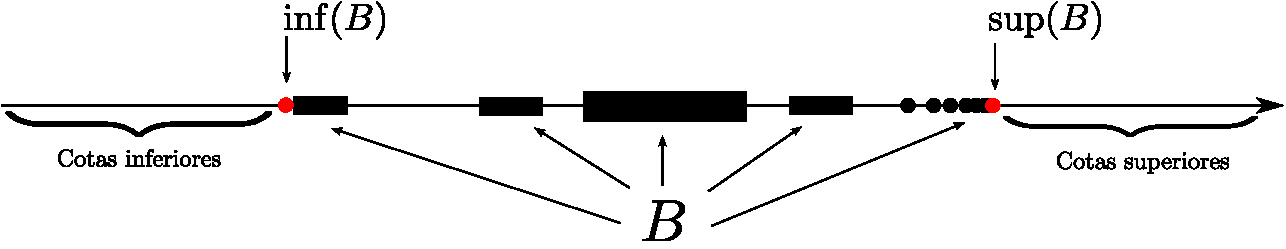
\includegraphics[width=0.98\linewidth]{Figuras/supremo-infimo}
% \caption{O supremo e o ínfimo de um conjunto $B$ limitado, representados pelo pontos indicados em vermelho. A direita indicamos os conjunto de todas as cotas superiores de $B$ e a esquerda o 
% conjunto de todas as cotas inferiores de $B$.}
% \label{fig:supremo-infimo}
% \end{figure}



% Dado um conjunto $B\subset \mathbb{R}$ defina o conjunto $-B\equiv \{-b\in\mathbb{R}: b\in B\}$.
% Então podemos verificar que se $B$ é um conjunto limitado (superiormente e inferiormente) então
% temos a seguinte igualdade 
% \[\inf(B) = - \sup(-B).\] 
% Desta forma as propriedades do ínfimo
% de conjuntos limitados podem ser obtidas por meio das propriedades do supremo e vice-versa.
% Esta equação poderia ter sido usada como definição de ínfimo. Apesar disto ter a vantagem
% de tornar a exposição mais curta, esta maneira acaba sendo pouco intuitiva para iniciantes.
% Além do mais conceitos introduzidos por negação de negação tendem a gerar bastante confusões. 

% Observamos que se levamos em conta as convenções listadas abaixo: 
% \begin{itemize}
% 	\item se $B$ não é limitado superiormente $\sup(B)=+\infty$;
% 	\item se $B$ não é limitado inferiormente $\inf(B)=-\infty$;
% 	\item $\sup \emptyset = -\infty$;
% 	\item $\inf \emptyset = +\infty$.
% \end{itemize} 
% então a igualdade $\inf(B) = - \sup(-B)$, 
% passa a ser válida para qualquer subconjunto $B\subset\mathbb{R}$.


% Por questão de conveniência relacionamos abaixo algumas propriedades do supremo e ínfimo
% que inevitavelmente serão usadas no texto. Antes, precisamos de algumas definições preliminares.
% A prova da validade das relações seguintes podem ser encontradas, por exemplo, em 
% \cite{MR0385023}. 

% \bigskip 


% Dados subconjuntos não-vazios arbitrários $A$ e $B$ contidos em $\mathbb{R}$ definimos
% \begin{itemize}
% 	\item $A+B\equiv \{ a+b\in\mathbb{R}: a\in A\ \text{e}\ b\in B\}$;
% 	\item $A\cdot C \equiv \{ a\cdot b\in\mathbb{R}: a\in A\ \text{e}\ b\in B\}$;
% 	\item $k\cdot A \equiv \{k\cdot a\in\mathbb{R}: a\in A \}$
% \end{itemize}



% \begin{teorema}\label{teo-prop-sup-inf}
% Sejam $A,B\subset \mathbb{R}$.
% \begin{enumerate}
	
% 	\item Se $A\subset B$ então $\sup(A)\leqslant \sup(B)$;
	
% 	\item Se $A\subset B$ então $\inf(B)\leqslant \inf(A)$;
	
% 	\item Se $B$ é limitado superiormente, então dado $\varepsilon>0$ existe $b\in B$ tal que 
% 	$\sup(B)<b+\varepsilon$; 
	
% 	\item Se $B$ é limitado inferiormente, então dado $\varepsilon>0$ existe $b\in B$ tal que\break
% 	$b-\varepsilon<\inf(B)$.  
	
% 	\item Se $A$ e $B$ são limitados superiormente então $\sup(A+B)=\sup(A)+\sup(B)$.
	
% 	\item Se $A$ e $B$ são limitados inferiormente então $\inf(A+B)=\inf(A)+\inf(B)$.
	
% 	\item Se $k\geqslant 0$ e $A$ limitado inferiormente então $\inf(k\cdot A)=k\inf(A)$.
	
% 	\item Se $k\geqslant 0$ e $A$ limitado superiormente então $\sup(k\cdot A)=k\sup(A)$.
	
% 	\item Se $k\leqslant 0$ e $A$ limitado superiormente então $\inf(k\cdot A)=k\sup(A)$.
	
% 	\item Se $k\leqslant 0$ e $A$ limitado inferiormente então $\sup(k\cdot A)=k\inf(A)$.
	
% 	\item Se $A,B\subset [0,+\infty)$ então $\inf(A\cdot B)= \inf(A)\cdot\inf(B)$;
	
% 	\item Se $A,B\subset [0,+\infty)$ então $\sup(A\cdot B)=\sup(A)\cdot\sup(B)$, 
% 	caso um dos conjuntos não seja limitado superiormente esta igualdade pode ser apenas  $+\infty=+\infty$.
% \end{enumerate}
% \end{teorema}

%\end{subappendices}
% Lista 2
%\chapter*{Lista 2}
\addcontentsline{toc}{chapter}{Lista 2}
\markboth{Lista 2}{Lista 2}
%%%%%%%%%%%%%%%%%%%%%%%%%%%%%%%%%%%%%%%%%%%%%%%%



% Inicio da Lista de Exercícios 
\begin{enumerate}[leftmargin=*]
	\item Neste exercício $z_0$ é um número complexo arbitrário fixado. 
	Esboce os conjuntos abaixo, diga se são fechados, abertos
	ou nenhum deles, esboce sua fronteira, diga quais são domínios e quais são limitados:
	\\
	a) $\Re(z)\geq \Re(z_0)$;\\
	b) $\Im(z_0)> \Re(z)$;\\
	c) $\Re(z^2)\geq 1$;\\
	d) $\Im(zz_0)>0$;\\
	e) $|z-z_0|<|\overline{z}-z_0|$;\\
	f) $|z-z_0|\leq |z-\overline{z_0}|$;\\
	g) $1\leq |z-\overline{z_0}|\leq 3$;\\
	h) $\Im(z^2)\leq 1$.
	\item Para cada um dos conjuntos abaixo sua fronteira é descrita 
	por uma curva suave por partes. Esboce o conjunto, sua fronteira e dê uma aplicação que a descreva\\
	a) $V=\{z\in\mathbb{C}: |z|\leq 1,\ \Re(z)\geq 1/2\}$;\\
	b) $V=\{z\in\mathbb{C}: 1/2\leq |z|\leq 1, \ \Re(z)\geq 0\}$;\\
	c) $V=\{z\in\mathbb{C}: 1/3\leq |z|\leq 1,\  \Re(z)\geq \Im(z)\geq 0\}$.

	\item Calcule a $\int_{\partial V} f$, onde $V$ é cada um dos conjuntos do exercício anterior ($V$ e a $\partial V$ tem orientação compatível) 
	e a função $f$ é dada por \\[0.2cm]
	a) $f(x,y)=\left(\displaystyle\frac{-y}{x^2+y^2},\frac{x}{x^2+y^2}\right)$;\\[0.3cm]
	b) $f(x,y)=\left(\displaystyle\frac{x}{x^2+y^2},\frac{-y}{x^2+y^2}\right)$;\\
	\item Calcule $\int_{\partial V}x^n\, dy$ e $\int_{\partial V}y^n\, dx$, onde $n\geq 1$ e $V$ é dado por \\
	a) o quadrado $[0,1]\times [0,1]$;\\
	b) o disco $\mathbb{D}\equiv \{z\in\mathbb{C}: |z|< 1\}$;\\ 
	levando em conta que $V$ e $\partial V$ estão compativelmente orientados.
	\item Seja $V$ como enunciado do Teorema de Green. Mostre que a área de $V$ é dada por 
	$$
	\int_{\partial V} x\, dy.
	$$
	\item Use o exercício anterior para calcular a área de\\
	a) $V=\{(x,y)\in\mathbb{R}^2: \frac{x^2}{a^2}+\frac{y^2}{b^2}\leq 1\}$;\\
	b) $V=\{(x,y)\in\mathbb{R}^2: 1\leq x^2-y^2\leq 9, \ 1\leq xy\leq 4\}$.
	\item Calcule 
	\\[0.2cm]
	a) $\displaystyle\int_{\partial V} (x^2-y^2)\, dx+ 2xy \, dy$\ ;\\[0.5cm]
	b) $\displaystyle \int_{\partial V} 2xy\, dx+ (y^2-x^2) \, dy$\ ,\\[0.5cm]
	onde $V$ é \\
	a) o retângulo delimitado pelas retas $y=x, y=-x+4, y=x+2, y=-x$;\\
	b) $\{(x,y)\in\mathbb{R}^2: 1\leq x^2-y^2\leq 9, \ 1\leq xy\leq 4\}$ ($V$ e $\partial V$ tem fronteira compatível). 
	\item Calcule 
	$$
	\int_{\partial V} \frac{y}{(x-1)^2+y^2}\ dx + \frac{x-1}{(1-x)^2+y^2}\ dy,
	$$
	onde $V$ é a região limitada pelos círculos $x^2+y^2=3$ e $(x-1)^2+y^2=9$ ($V$ e $\partial V$ tem fronteira compatível). 
	\item Calcule 
	$$
	\int_{\partial V} \frac{x^2y}{(x^2+y^2)^2}\ dx - \frac{x^3}{(x^2+y^2)^2}\ dy,
	$$
	onde $V$ é a região interior a elipse $\frac{x^2}{4}+\frac{y^2}{9}=1$ orientada no sentido anti-horário. 


\end{enumerate}

% Semana 3
%% !TeX spellcheck = pt_BR
\chapter[Semana 3]{}
\chaptermark{}



\hfill%
\begin{minipage}{12cm}
	\begin{flushright}
		\rightskip=0.5cm
		\textit{``At the basis of the distance concept lies, for example, 
		the concept of a convergent point sequence and their defined limits,
		and one can, choosing these ideas as those fundamental to the point 
		set theory, eliminate the notions of distance ... Thirdly, 
		we can associate with each point of the set certain parts of the space
		called neighborhoods, and these can again be made building stones of the 
		theory with the elimination of the distance concept. Here the view
		of a set is in consideration of the association between elements and
		subsets.''}
		\\[0.1cm]
		\rightskip=0.5cm
		---F. Hausdorff, 1949
	\end{flushright}
\end{minipage}




\section{Limites, Continuidade de Funções Complexas}

Uma função complexa é uma função $f:U\subset \mathbb{C}\to\mathbb{C}$ definida em algum 
subconjunto $U\subset \mathbb{C}$ e tomando valores em $\mathbb{C}$
que associa cada ponto $z\in U$ um número complexo $f(z)$.
Podemos também descrever tais funções usando coordenadas, isto é,
para $z=x+iy\in U$ temos 
$f(z)=f(x+iy)=u(x,y)+iv(x,y)$, onde $u(x,y)=\Re(f(x+iy))=$ e $v(x,y)=\Im(f(x+iy))$.


Por exemplo, a função $f:\mathbb{C}\to\mathbb{C}$ dada por $f(z)=z^2$ pode ser
descrita em coordenadas por 
$f(x+iy) = (x+iy)^2 = x^2-y^2+2ixy$.
Em geral, é prudente evitar trabalhar com coordenadas. 
Mas isto não quer dizer que não devemos usá-las, mas sim 
avaliar cuidadosamente se uso delas facilitará ou viabilizará o estudo 
do problema. Um dos resultados mais importantes da próxima seção
às chamadas Condições de Cauchy-Riemann, fornecem um exemplo 
importante de como a descrição de uma função complexa em termos de suas coordenadas
pode ser poderosa. 

\bigskip 

A noção de limite associado a uma função $f:A\subset \mathbb{C}\to\mathbb{C}$ 
consiste simplesmente numa tradução da Definição \ref{definicao-limite-R2}.
Por questão de simplicidade, como na seção anterior, vamos considera apenas 
funções definidas em algum conjunto $A\subset\mathbb{C}$
cujo o interior é não-vazio. 

\begin{definicao}\label{def-limite-func-complexa}
\index{Limite!de uma função complexa}
Sejam $A\subset \mathbb{C}$ um conjunto cujo interior é não-vazio, $f:A\to\mathbb{C}$ uma 
função e $z_0\in \overline{A}$. Dizemos que um número complexo $w_0$ 
é o limite de $f(z)$ quando $z$ tende a $z_0$ se, dado qualquer $\varepsilon>0$ é possível
encontrar $\delta>0$ tal que se $z\in A$ e  $0<|z-z_0|<\delta$ então  temos $|f(z)-w_0|<\varepsilon$.
O limite será denotado por
\[
\lim_{z\to z_0} f(z) = w_0\qquad \text{ou} \qquad f(z)\xrightarrow{\ z\to z_0\ }w_0.
\]
\end{definicao}
É comum referir-se ao fato de que $f(z)\xrightarrow{\ z\to z_0\ }w_0$, dizendo simplesmente
que $f(z)$ converge para $w_0$, quando $z$ tende a $z_0$.

A intuição deste conceito de limite é totalmente análoga a de limite de funções em $\mathbb{R}^2$.
Ou seja, dado qualquer $\varepsilon>0$ podemos encontrar um $\delta\equiv \delta(\varepsilon,z_0)$ 
tal que todo ponto $z$ que está $\delta$-próximo de $z_0$ é enviado por $f$ $\varepsilon$-próximo de $w_0$.

\begin{exemplo}
Seja $f:\mathbb{C}\to\mathbb{C}$ dada por $f(z)=z^2$.  Seja $z_0=i$. Então, segundo a definição acima 
temos 
\[
\lim_{z\to i } f(z) = -1.
\]
De fato, dado $\varepsilon>0$, tome $\delta = \sqrt{1+\varepsilon} -1$. Desta forma, sempre que tomamos
$z$ tal que $|z-(-i)|<\delta$, temos
\begin{align*}
|z^2-(-1)|=|z^2+1|= |(z+i)(z-i)| 
&= |z+i|\cdot |z-i|
\\
&<
(\sqrt{1+\varepsilon} -1) |z-i|
\\
&=
(\sqrt{1+\varepsilon} -1) |z+i-2i|
\\
&\leqslant
(\sqrt{1+\varepsilon} -1) (|z+i|+|2i|)
\\
&<
(\sqrt{1+\varepsilon} -1) (\sqrt{1+\varepsilon} -1+2)
\\
&=
(\sqrt{1+\varepsilon} -1) (\sqrt{1+\varepsilon} +1)
\\
&=
(\sqrt{1+\varepsilon})^2-1^2
\\
&=
\varepsilon.
\end{align*}
\end{exemplo}

Uma propriedade muito importante e naturalmente esperada de qualquer definição de limite é que o mesmo
seja único. Neste caso é simples verificar a unicidade do limite, basta aplicar a desigualdade triangular como
segue. Se $f(z)\to w_0$, quando $z\to z_0$ e $f(z)\to w_1$, quando $z\to z_0$, então dado $\varepsilon>0$
sabemos que existe $\delta>0$ tal que se $0<|z-z_0|<\delta$ 
então $|f(z)-w_0|<\varepsilon/2$ e $|f(z)-w_1|<\varepsilon/2$.
Logo $|w_0-w_1| = |w_0-f(z)+f(z)-w_1|\leq |f(z)-w_0|+|f(z)-w_1|<\varepsilon/2+\varepsilon/2 = \varepsilon$.
Para a desigualdade acima ser válida para todo $\varepsilon$ é necessário que $|w_0-w_1|=0$, o que queríamos
demonstrar.


\bigskip

O limite de uma função complexa pode ser expresso também em termos de suas coordenadas. Em outras palavras, 
uma função complexa tem limite se, e somente se, suas partes real e imaginária
têm limite. Mais precisamente, se escrevemos $f(z)=u(x,y)+iv(x,y)$, onde $z=x+iy$ e se existe 
o limite $\lim_{z\to z_0}f(z)=w_0$, onde $z_0=x_0+iy_0$ e $w_0=u_0+iv_0$, então temos
\begin{align*}
\lim_{(x,y)\to (x_0,y_0)} u(x,y) = u_0
\qquad\text{e}\qquad 
\lim_{(x,y)\to (x_0,y_0)} v(x,y) = v_0.
\end{align*}

Para verificar que ambas igualdades vamos aplicar o Lema \ref{lema-re-im-modulo} que 
garante
\[
|u(x,y)-u_0|\leqslant |f(z)-w_0|
\qquad \text{e}\qquad 
|v(x,y)-v_0|\leqslant |f(z)-w_0|.
\]
Assim, dado $\varepsilon>0$, existe $\delta>0$ tal que 
se $z\in A$ e  $|z-z_0|<\delta$ (ou  $\|(x,y)-(x_0,y_0)\|<\delta$), 
então $|f(z)-w_0|<\varepsilon$. Logo segue das últimas duas desigualdades que $|u(x,y)-u_0|<\varepsilon$
e $|v(x,y)-v_0|<\varepsilon$ o que prova a afirmação sobre os limites das funções coordenadas $u$ e $v$.
A recíproca pode ser provada de forma análoga simplesmente substituindo o argumento do Lema \ref{lema-re-im-modulo}
pela desigualdade triangular.

As propriedades do limite de uma função complexa são análogas às do limite de funções reais, já que 
tudo que são usadas em ambas definições são as estruturas de distância (que na reta é definida pelo valor absoluto e no 
plano complexo pela norma) e de corpo. Relacionamos abaixo algumas das mais básicas e úteis:


\begin{lema}\label{lema-limite-f-limitada}
Seja  $A\subset \mathbb{C}$ conjunto de interior não-vazio, $f:A\to\mathbb{C}$ uma função complexa
e $z_0\in \overline{A}$. Suponha 
\[
\lim_{z\to z_0} f(z) = w_0.
\]
Então existe algum $r>0$ tal que $f$ é limitada no conjunto $V(A,r)\equiv \{z\in A: 0<|z-z_0|<r\}$,
isto é, existe uma constante $M$ (que pode depender de $z_0$ e $r$) tal que   $|f(z)|\leq M$
para todo $z\in V(A,r)$.
\end{lema}
\begin{proof}
Pela definição de limite, dado $\varepsilon=1$ existe $\delta>0$ tal que para todo $z\in A$ com 
$0<|z-z_0|<\delta$, temos $|f(z)-w_0|<1$. Pela segunda desigualdade triangular segue que 
$|f(z)|-|w_0|\leqslant |f(z)-w_0|<1$, o que implica que $|f(z)|\leqslant 1+|w_0|$. 
Para finalizar a prova basta tomar $M\equiv 1+|w_0|$ e $r=\delta$.
\end{proof}


\begin{proposicao}\label{prop-propriedades-limite-funcao-complexa}
Sejam $A\subset \mathbb{C}$ conjunto de interior não-vazio, $f_1,f_2:A\to\mathbb{C}$ duas funções complexas
e $z_0\in \overline{A}$. Se 
\[
\lim_{z\to z_0} f_1(z) = w_1\qquad\text{e}\qquad \lim_{z\to z_0} f_2(z) = w_2
\]
então 
\begin{enumerate}
\item $\displaystyle \lim_{z\to z_0} cf_1(z) = c \lim_{z\to z_0} f_1(z) = cw_1$, onde $c$ é uma constante complexa;
\item $\displaystyle \lim_{z\to z_0} (f_1(z)+f_2(z)) = \lim_{z\to z_0} f_1(z) + \lim_{z\to z_0}f_2(z) = w_1+w_2$;
\item $\displaystyle \lim_{z\to z_0} (f_1(z)\cdot f_2(z)) = \lim_{z\to z_0} f_1(z) \cdot \lim_{z\to z_0}f_2(z) = w_1\cdot w_2$;
\item se $w_1\neq 0$ então $\displaystyle \lim_{z\to z_0}\frac{1}{f_1(z)} = \frac{1}{w_1}$.
\end{enumerate}
\end{proposicao}

\begin{proof}
Vamos provar os itens $\mathit{2}$ e $\mathit{3}$. A prova dos itens restantes é semelhante. 

Prova do item $\mathit{2}$. Pela definição de limite, dado $\varepsilon>0$ existem $\delta_1,\delta_2>0$ tais que se $|z-z_0|<\delta_1$
então $|f_1(z)-w_1|<\varepsilon/2$ e se $|z-z_0|<\delta_2$ então $|f_2(z)-w_2|<\varepsilon/2$.
Portanto, se $|z-z_0|<\delta\equiv \min\{\delta_1,\delta_2\}$ temos da desigualdade triangular que  
\[
|f_1(z)+f_2(z) - (w_1+w_2)|\leqslant |f_1(z)-w_1|+|f_2(z)-w_2| <\frac{\varepsilon}{2}+\frac{\varepsilon}{2} = \varepsilon,
\]
mostrando que $f_1(z)+f_2(z)\xrightarrow{\ z\to z_0\ }w_1+w_2$.

Prova do item $\mathit{3}$. Pela definição de limite dado $\varepsilon>0$ sabemos que existe $\delta_1>0$
tal que se $|z-z_0|<\delta_1$, então $|f_1(z)-w_1|<\varepsilon/2|w_2|$. Pelo Lema \ref{lema-limite-f-limitada}
existem $\delta_2>0$ e uma constante $M>0$ tal que se $|z-z_0|<\delta_2$, então $|f_1(z)|\leqslant M$.
Também pela definição de limite podemos encontrar $\delta_3>0$ tal que se $|z-z_0|<\delta_3$ 
então $|f_2(z)-w_2|<\varepsilon/2M$. Aplicando a desigualdade triangular temos
\begin{align*}
|f_1(z)f_2(z) - w_1w_2 | &=  |f_1(z)f_2(z)- f_1(z)w_2+f_1(z)w_2-w_1w_2|
\\
&\leqslant 
|f_1(z)f_2(z)- f_1(z)w_2|+|f_1(z)w_2-w_1w_2|
\\
&=
|f_1(z)|\, |f_2(z)-w_2| + |w_2|\, |f_1(z)-w_1|
\\
&\leqslant
M \frac{\varepsilon}{2M}+|w_2| \frac{\varepsilon}{2|w_2|}
=
\varepsilon.
\end{align*}
Mostrando assim que $f_1(z)\cdot f_2(z)\xrightarrow{\ z\to z_0\ }w_1\cdot w_2$.
\end{proof}

De maneira semelhante às funções de $\mathbb{R}ˆ2$ definimos o conceito de continuidade.  

\begin{definicao}[Função Contínua]
\label{def-func-complexa-continua}
\index{Função!contínua}
Sejam $A\subset \mathbb{C}$ um aberto e $f:A\to\mathbb{C}$ uma função. Dizemos que 
$f$ é contínua em $z_0\in A$ se 
\[
\lim_{z\to z_0} f(z) = f(z_0).
\]
Se $f$ é contínua em todo ponto $z_0\in A$, dizemos que $f$ é contínua em $A$.
\end{definicao}

Note que a continuidade de uma função complexa é equivalente a continuidade de 
suas funções coordenadas. Isto é, $f:A\to\mathbb{C}$ é contínua se, e somente se,
as funções $z\longmapsto \Re(z)$ e $z\longmapsto \Im(z)$ são contínuas em $A$.

Podemos também verificar diretamente à partir da definição 
que $f:\mathbb{C}\to\mathbb{C}$ dada por $f(z)=\overline{z}$ é uma função contínua em $\mathbb{C}$.
Usando a proposição anterior podemos também verificar facilmente que 
a função $g:\mathbb{C}^{*}\to\mathbb{C}$ dada por $g(z) = 1/z$ é contínua em $\mathbb{C}^{*}$.

A seguir vamos mostrar que uma versão da  Proposição \ref{prop-propriedades-limite-funcao-complexa}
para o caso de funções contínuas. Além disto vamos incluir nesta nova proposição uma afirmação sobre
a continuidade de composições e para isto vamos relembrar o conceito de composição de funções. 
Sejam $A,B\subset \mathbb{C}$ conjuntos abertos, $f:B\to\mathbb{C}$ e $g:A\to\mathbb{C}$
funções tais que $g(A)\subset B$. Sob estas condições podemos definir a função composta $f\circ g: A\to\mathbb{C}$
pela expressão $f\circ g(z) \equiv f(g(z))$, para cada $z\in A$.

\begin{proposicao}
Sejam $A,B\subset \mathbb{C}$ abertos e $f_1:B\to\mathbb{C}$, $f_2:B\to\mathbb{C}$ e $g:A\to\mathbb{C}$ 
funções complexas tais que $g(A)\subset B$. Suponha que $f_1$ e $f_2$ são contínuas em $z_0\in B$ e
que $f_1$ é contínua em $g(z_1)$, onde $z_1\in A$. Então 
\begin{enumerate}
	\item são contínuas em $z_0\in B$ as funções:
		\begin{itemize}
			\item  $cf_1:B\to\mathbb{C}$; 
			\item  $f_1+f_2:B\to\mathbb{C}$;
			\item $f_1\cdot f_2: B\to\mathbb{C}$.
		\end{itemize}

	\item se $f_1(z_0)\neq 0$ então a função $\displaystyle\frac{1}{f_1}:B\setminus\{z\in B: f_1(z)=0\} \to \mathbb{C}$
	é contínua em $z_0$;
	
	\item a função $f_1\circ g :A\to\mathbb{C}$ é contínua em $z_1$.
\end{enumerate}
\end{proposicao}

\begin{proof}
As provas dos itens $\mathit{1}$ e $\mathit{2}$ são idênticas aos respectivos itens da Proposição \ref{prop-propriedades-limite-funcao-complexa} por isto faremos apenas a prova do item $\mathit{3}$.
Dado $\varepsilon>0$ segue da continuidade de $f_1$ no ponto $g(z_1)$, 
que existe $\delta_1>0$ tal que se $|w-g(z_1)|<\delta_1$
então $|f_1(w)-f_1(g(z_1))|<\varepsilon$. Pela continuidade de $g$ em $z_1$ podemos encontrar $\delta_2>0$
tal que se $|z-z_1|<\delta_2$ então $|g(z)-g(z_1)|<\delta_1$. Assim,
tomando $\delta=\delta_2$ temos que se 
 se $|z-z_1|<\delta$ então $|f_1(g(z))-f_1(g(z_1))|<\varepsilon$.
\end{proof}


\section{A Derivada Complexa}

Nesta seção vamos definir a derivada complexa de uma função $f:A\subset\mathbb{C}\to\mathbb{C}$.
Para facilitar vamos trabalhar apenas com funções definidas em subconjuntos abertos de $\mathbb{C}$.
A noção de derivada complexa é uma noção que diferencia o cálculo de variáveis reais e complexas.
A partir dela veremos surgir uma teoria de cálculo diferencial completamente nova e rica de propriedades
interessantes. As novidades oriundas desta nova noção de derivada 
fazem desta, uma teoria extremamente útil em diversas aplicações em matemática pura e aplicada, 
física, engenharia e muitas outras áreas.

\begin{definicao}\label{def-derivada-complexa}
\index{Derivada!complexa}
Sejam $A\subset\mathbb{C}$ um aberto e $f:A\to\mathbb{C}$ uma função. Dizemos que $f$
tem derivada no sentido complexo em $z_0\in A$ se existe o seguinte limite 
\[
f'(z_0) \equiv \lim_{z\to z_0} \frac{f(z)-f(z_0)}{z-z_0}.
\]
\end{definicao}

A diferença marcante aqui é que apesar da derivada ser definida como no caso de funções reais,
pelo limite de quocientes de Newton, agora o quociente de Newton é tomado no sentido da divisão 
de números complexos. Esta que parece uma pequena diferença terá consequências fantásticas!

Observamos que analogamente ao caso de funções reais a derivada complexa
pode também ser obtida  pelo seguinte limite 
\[
f'(z_0) = \lim_{h\to 0} \frac{f(z_0+h)-f(z_0)}{h}.
\]

Abaixo analisamos a existência da derivada complexa de duas funções bastante simples e importantes
neste texto.

\begin{exemplo}
A função $f:\mathbb{C}\to\mathbb{C}$ tem derivada complexa em qualquer $z_0\in\mathbb{C}$, além do mais
$f'(z_0)=2z_0$. 
Para verificar este fato, basta observar que 
\[
\lim_{z\to z_0}\frac{ f(z)-f(z_0)}{z-z_0} 
=
\lim_{z\to z_0} \frac{z^2-z_0^2}{z-z_0}
=
\lim_{z\to z_0} \frac{(z-z_0)(z+z_0)}{z-z_0}
=
\lim_{z\to z_0} z+z_0
=
2z_0.
\]
\end{exemplo}
 
O próximo exemplo mostra como a derivada complexa pode ser radicalmente diferente da derivada 
no sentido real. 

\begin{exemplo}
Considere a função $f:\mathbb{C}\to\mathbb{C}$ dada por $f(z)=\overline{z}$, para todo $z\in\mathbb{C}$.
Então não existe nenhum ponto do plano complexo onde esta função tenha derivada.

Para verificar este fato vamos considerar $z_0$ um ponto arbitrário fixado e o quociente de Newton 
\begin{align*}
\frac{f(z)-f(z_0)}{z-z_0}
&=
\frac{\overline{z}-\overline{z_0}}{z-z_0}
\\
&=
\frac{\overline{z}-\overline{z_0}}{z-z_0} \cdot \frac{\overline{z}-\overline{z_0}}{\overline{z}-\overline{z_0}}
=
\frac{(\overline{z}-\overline{z_0})^2}{|z-z_0|^2} 
\\
&=
\frac{(x-x_0+i(y-y_0))^2}{(x-x_0)^2+(y-y_0)^2}
\\
&=
\frac{(x-x_0)^2-(y-y_0)^2+2i(x-x_0)(y-y_0)}{(x-x_0)^2+(y-y_0)^2}.
\end{align*}
Agora vamos fazer $z$ se aproximar de $z_0$ por retas paralelas aos eixos coordenados que passando por 
$z_0$.

Primeiro consideramos  $z$ da forma $z=t+iy_0$, onde $t\in\mathbb{R}$. Neste caso obtemos, das identidades acima,
para $t\neq x_0$ a seguinte igualdade
\begin{align*}
\frac{f(t+iy_0)-f(z_0)}{(t+iy_0)-z_0}
&=
\frac{(t-x_0)^2-(y_0-y_0)^2+2i(t-x_0)(y_0-y_0)}{(t-x_0)^2+(y_0-y_0)^2}
\\
&=
\frac{(t-x_0)^2}{(t-x_0)^2}=1.
\end{align*}

Por outro lado, se consideramos $z$ da forma $z=x_0+it$, onde $t\in\mathbb{R}$ temos para $t\neq y_0$
\begin{align*}
\frac{f(x_0+it)-f(z_0)}{(x_0+it)-z_0}
&=
\frac{(x_0-x_0)^2-(t-y_0)^2+2i(x_0-x_0)(t-y_0)}{(x_0-x_0)^2+(t-y_0)^2}
\\
&=
-\frac{(t-y_0)^2}{(t-y_0)^2}=-1.
\end{align*}
Como os limite quando $z$ tende a $z_0$ do quociente de Newton ao longo destes dois caminhos é distinto
segue que não pode existir a derivada de $f$ no ponto $z_0$. Mas já que $z_0$ é arbitrário, concluímos que
esta função não tem derivada em nenhum ponto do plano complexo.
\end{exemplo}

O exemplo acima, mostra como o conceito de derivada complexa é novo. Além do mais ele mostra
que em $\mathbb{C}$ é muito simples construir um função que é contínua em todos pontos
mas não é derivável em ponto algum. Existem funções com propriedades semelhantes definidas da reta na reta,
mas são muito mais complicadas de serem construídas. 


\begin{proposicao}\label{prop-diferenciavel-continua}
Sejam $A\subset\mathbb{C}$ um aberto e  $f:A\to\mathbb{C}$ uma função derivável em $z_0\in A$.
Então $f$ é contínua em $z_0$.
\end{proposicao}
\begin{proof}
Basta observar que 
\begin{align*}
\lim_{z\to z_0} (f(z)-f(z_0))
&=
\lim_{z\to z_0} (f(z)-f(z_0))\, \frac{z-z_0}{z-z_0}
\\
&=
\lim_{z\to z_0}  (z-z_0)\, \frac{f(z)-f(z_0)}{z-z_0}
\\
&=
0\cdot f'(z_0)=0.
\end{align*}
\end{proof}


\begin{proposicao}\label{prop-derivada}
Sejam $A\subset\mathbb{C}$ um aberto, $f$ e $g$ funções diferenciáveis em $z_0\in A$. 
Então temos 
\begin{enumerate}
	\item $(cf)'(z_0) = cf'(z_0)$, para qualquer constante $c\in\mathbb{C}$;
	\item $(f+g)'(z_0) = f'(z_0)+g'(z_0)$;
	\item $(f\cdot g)'(z_0) = f'(z_0)g(z_0)+f(z_0)g'(z_0)$;
	\item $\displaystyle\left( \frac{1}{f} \right)'(z_0) = -\frac{f'(z_0)}{f(z_0)^2}$, se $f(z_0)\neq 0$.
	\item $\displaystyle\left( \frac{f}{g} \right)'(z_0) = \frac{f'(z_0)g(z_0)-f(z_0)g'(z_0)}{g(z_0)^2}$, se $g(z_0)\neq 0$.
\end{enumerate}
\end{proposicao}

\begin{proof}
A prova dos itens $\mathit{1},\ \mathit{2}$ e $\mathit{3}$ são semelhantes a das proposições anteriores.
Por isto vamos apresentar somente a prova dos itens $\mathit{4}$ e $\mathit{5}$.

Para provar $\mathit{4}$ primeiro observamos que podemos reescrever o 
quociente de Newton de $1/f$ como segue já que  $f(z_0)\neq 0$. 
\begin{align*}
\frac{ \displaystyle \frac{1}{f(z)}  -  \frac{1}{f(z_0)}  }{z-z_0}
=
\frac{ \displaystyle  \frac{ f(z_0)-f(z) }{ f(z)f(z_0) }    }{z-z_0}
=
- \frac{1}{f(z)f(z_0)}\cdot   \frac{f(z)-f(z_0)}{z-z_0},
\end{align*}
Como estamos assumindo que $f$ é derivável em $z_0$ segue da Proposição \ref{prop-diferenciavel-continua}
que $f$ é contínua em $z_0$. Desta forma podemos tomar o limite, quando $z$ tende a $z_0$ na expressão 
à direita da igualdade acima obtendo 
\[
\lim_{z\to z_0} \frac{ \displaystyle \frac{1}{f(z)}  -  \frac{1}{f(z_0)}  }{z-z_0}
 = 
- \lim_{z\to z_0} \frac{1}{f(z)f(z_0)}\cdot   \frac{f(z)-f(z_0)}{z-z_0}
=
-\frac{f'(z_0)}{f(z_0)^2}.
\]

A prova do item $\mathit{5}$. Já que estamos assumindo que $g$ é derivável em $z_0$ e também $g(z_0)\neq 0$
podemos aplicar os itens $\mathit{3}$ e $\mathit{4}$ para concluir que 
\begin{align*}
\left( \frac{f}{g} \right)'(z_0) 
=
\left( f \cdot \frac{1}{g}\right)'(z_0)
&=
f'(z_0) \frac{1}{g(z_0)} + f(z_0)\left( \frac{1}{g}\right)'(z_0)
\\[0.3cm]
&=
 \frac{f'(z_0)}{g(z_0)}  -f(z_0)\frac{g'(z_0)}{g(z_0)^2}
\\[0.2cm]
&=
\frac{f'(z_0)g(z_0)-f(z_0)g'(z_0)}{g(z_0)^2}. 
\end{align*} 
\end{proof}

\begin{teorema}[Regra da Cadeia]
\label{teo-regra-da-cadeia}
\index{Regra da Cadeia}
Sejam $A, B$ abertos de $\mathbb{C}$ e $f:B\to\mathbb{C}$ e $g:A\to\mathbb{C}$ funções tais que $g(A)\subset B$.
Se $g$ é derivável em $z_0$ e $f$ é derivável em $f(g(z_0))$, então 
\[
(f\circ g)'(z_0) = f'(g(z_0))g'(z_0).
\]
\end{teorema}

\begin{proof}
Defina a função $h:B\to\mathbb{C}$ como segue
\[
h(w)
=
\begin{cases}
\displaystyle\frac{f(w)-f(g(z_0))}{w-g(z_0)}- f'(g(z_0)),&\text{se}\ w\neq g(z_0);\\
0,&\text{se}\ w=g(z_0).
\end{cases} 
\]
Observe que $h$ está bem definida em $B$ e é contínua em $g(z_0)$
uma vez que $f$, por hipótese, é derivável em $g(z_0)$. 
Como também é continuidade $g$ em $z_0$, temos
\begin{align}\label{eq-aux1-regra-cadeia}
\lim_{z\to z_0} (h\circ g)(z) = h(g(z_0))=0.
\end{align}
Para todo $w\in B$ temos a seguinte igualdade (válida também para $w=g(z_0)$)
\[
f(w)-f(g(z_0))= ( h(w)+f'(g(z_0)))\,(w-g(z_0)).
\]
Substituindo $w$ por $g(z)$ na identidade acima e dividindo ambos os lados por $z-z_0$ obtemos:
\[
\frac{ f(g(z)) - f(g(z_0))  }{ z-z_0 } 
=  
\big(  h(g(z))+ f'(g(z_0))   \big) 
\,\frac{g(z)-g(z_0)}{z-z_0}.
\]
Lembrando de \eqref{eq-aux1-regra-cadeia}  
podemos concluir  da expressão do lado direito da igualdade acima que existe a derivada de $f\circ g$
em $z_0$ e temos
\begin{align*}
(f\circ g)'(z_0)
&=
\lim_{z\to z_0}
\frac{ f(g(z)) - f(g(z_0))  }{ z-z_0 } 
\\[0.2cm]
&=  
\lim_{z\to z_0}
\big(  h(g(z))+ f'(g(z_0))   \big) \frac{g(z)-g(z_0)}{z-z_0}
\\[0.2cm]
&=
f'(g(z_0))g'(z_0).
\qedhere
\end{align*}
\end{proof}


\section{As Condições de Cauchy-Riemann}

Nesta seção vamos analisar algumas das consequências da existência da derivada complexa.
Em particular, estaremos interessados nas propriedades funções coordenadas de uma função 
que tem derivada complexa em uma certa região do plano complexo. Um dos resultados
principais são as condições de Cauchy-Riemann e sua recíproca enunciados na sequência.

\begin{proposicao}[Condições de Cauchy-Riemann]
\label{prop-cond-Cauchy-Riemann}
\index{Condições!de Cauchy-Riemann}
Seja $A\subset \mathbb{C}$ um aberto, $z_0=x_0+iy_0\in A$ e $f:A\to\mathbb{C}$
uma função da forma $f(x+iy)=u(x,y)+iv(x,y)$  derivável em $z_0$. Então
\[
\frac{\partial}{\partial x}u(x_0,y_0)=\frac{\partial}{\partial y}v(x_0,y_0)
\quad\text{e}\quad
\frac{\partial}{\partial x}v(x_0,y_0)=-\frac{\partial}{\partial y}u(x_0,y_0).
\]
\end{proposicao}

\begin{proof}
Primeiro passo é expressar em coordenadas o quociente de Newton de $f$ como segue:
\begin{align*}
\frac{f(z)-f(z_0)}{z-z_0}
&=
\frac{u(x,y)-u(x_0,y_0)+i(v(x,y)-v(x_0,y_0))}{x-x_0+i(y-y_0)}
\\[0.3cm]
&=
\frac{u(x,y)-u(x_0,y_0)+i(v(x,y)-v(x_0,y_0))}{x-x_0+i(y-y_0)}\cdot \frac{x-x_0-i(y-y_0)}{x-x_0-i(y-y_0)}
\\[0.3cm]
&=
\frac{u(x,y)-u(x_0,y_0)+i(v(x,y)-v(x_0,y_0))}{(x-x_0)^2+(y-y_0)^2}\cdot\big(x-x_0-i(y-y_0)\big)
\\[0.3cm]
&=
\frac{(u(x,y)-u(x_0,y_0))(x-x_0)+(v(x,y)-v(x_0,y_0))(y-y_0)}{(x-x_0)^2+(y-y_0)^2}
\\
&\quad +i
\frac{(v(x,y)-v(x_0,y_0))(x-x_0)-(u(x,y)-u(x_0,y_0))(y-y_0)}{(x-x_0)^2+(y-y_0)^2}.
\end{align*}

Já que estamos assumindo que $f$ é diferenciável em $z_0$ o limite, quando $z\to z_0$, 
do quociente de Newton acima existe e é independente do caminho.
Desta forma podemos tomá-lo ao longo dos segmentos de reta passando por $z_0$ e paralelos aos eixos 
coordenados. 

Tomando o limite, na igualdade acima, quando $z\to z_0$ ao longo da reta $t+iy_0$, com $t\to x_0$ obtemos
\begin{align*}
f'(z_0)
&=
\lim_{t\to x_0} 
\frac{f(t+iy_0)-f(z_0)}{t+iy_0-(x_0+iy_0)}
\\[0.3cm]
&=
\lim_{t\to x_0} 
\frac{(u(t,y_0)-u(x_0,y_0))(t-x_0)+(v(t,y_0)-v(x_0,y_0))(y_0-y_0)}{(t-x_0)^2+(y_0-y_0)^2}
\\
&\quad +i \lim_{t\to x_0} 
\frac{(v(t,y_0)-v(x_0,y_0))(t-x_0)-(u(t,y_0)-u(x_0,y_0))(y_0-y_0)}{(t-x_0)^2+(y_0-y_0)^2}
\\[0.3cm]
&=
\lim_{t\to x_0} 
\frac{u(t,y_0)-u(x_0,y_0)}{t-x_0} 
+i \lim_{t\to x_0} 
\frac{v(t,y_0)-v(x_0,y_0)}{t-x_0}
\\[0.3cm]
&=
\frac{\partial }{\partial x}u(x_0,y_0) + i\frac{\partial }{\partial x}v(x_0,y_0).
\end{align*}

Repetindo o procedimento acima, mas agora fazendo $z$ tender a $z_0$ pela reta 
$x_0+it$, com $t\to y_0$ temos

\begin{align*}
f'(z_0)
&=
\lim_{t\to y_0} 
\frac{f(x_0+it)-f(z_0)}{x_0+it-(x_0+iy_0)}
\\[0.3cm]
&=
\lim_{t\to y_0} 
\frac{(u(x_0,t)-u(x_0,y_0))(x_0-x_0)+(v(t,y_0)-v(x_0,y_0))(t-y_0)}{(x_0-x_0)^2+(t-y_0)^2}
\\
&\quad +i \lim_{t\to y_0} 
\frac{(v(x_0,t)-v(x_0,y_0))(x_0-x_0)-(u(x_0,t)-u(x_0,y_0))(t-y_0)}{(x_0-x_0)^2+(t-y_0)^2}
\\[0.3cm]
&=
\lim_{t\to y_0} 
\frac{v(x_0,t)-v(x_0,y_0)}{t-y_0} 
-i \lim_{t\to x_0} 
\frac{u(t,y_0)-u(x_0,y_0)}{t-y_0}
\\[0.3cm]
&=
\frac{\partial }{\partial y}v(x_0,y_0) -i \frac{\partial }{\partial y}u(x_0,y_0).
\end{align*}

Dos dois últimos conjuntos de igualdades segue o resultado.
\end{proof}

Uma maneira muito prática de lembrar das condições de Cauchy-Riemann consistem em lembrar que 
$f$ vista como função de $\mathbb{R}^2$ em $\mathbb{R}^2$ tem derivada total representada
por sua matriz Jacobiana (matriz dos gradientes das funções coordenadas) $2\times 2$ como mostrado abaixo:
\[
Df(x_0,y_0)
=
\begin{pmatrix}
\displaystyle \frac{\partial}{\partial x}u(x_0,y_0) & \displaystyle \frac{\partial}{\partial y} u(x_0,y_0)
\\[0.5cm] 
\displaystyle \frac{\partial}{\partial x}v(x_0,y_0) & \displaystyle \frac{\partial}{\partial y} v(x_0,y_0)
\end{pmatrix}.
\]
Desta forma para que este Jacobiano represente um número complexo e necessário que ele seja da forma 
\[
\begin{pmatrix}
a&b\\
-b&a
\end{pmatrix}
\]
o que se traduz precisamente nas condições de Cauchy-Riemann.

\bigskip 

Como vimos acima as condições de Cauchy-Riemann são necessárias para que $f$ seja derivável em um 
ponto $z_0$ em seu domínio. Mas o exemplo abaixo mostra que elas podem, em geral, não ser suficientes
para garantir a existência da derivada complexa

\begin{exemplo}
A função $f:\mathbb{C}\to\mathbb{C}$ dada por 
\[
f(x+iy)
=
\begin{cases}
0,& \text{se}\ xy=0;
\\
1,& \text{se}\ xy\neq 0.
\end{cases}
\]
satisfaz as condições de Cauchy-Riemann em $z_0=0$, pois as derivadas parciais das funçoões coordenadas $u$ e $v$
são nulas na origem. Porém ela não pode ter derivada complexa na origem
já que ela não é nem mesmo contínua neste ponto.
\end{exemplo}

Uma condição razoavelmente geral que a garante a existência da derivada complexa de uma função $f$
satisfazendo as condições de Cauchy-Riemann será dada na próxima proposição. Mas para prová-la
vamos precisar do seguinte lema auxiliar

\begin{lema}\label{lema-aux-reciproca-CR}
Sejam $A\subset\mathbb{R}^2$ aberto e $F:A\to\mathbb{R}$ uma função admitindo derivadas parciais contínuas 
em $(x_0,y_0)\in A$. Então temos 
\begin{align}\label{eq-aux1-lema-aux-reciproca-CR}
F(x,y)-F(x_0,y_0)
&=
(x-x_0)\left(  \frac{\partial }{\partial x}F(x_0,y_0) +H(x-x_0,y-y_0) \right)
\\
&\quad +
(y-y_0)\left(  \frac{\partial }{\partial y}F(x_0,y_0) +K(x-x_0,y-y_0) \right),
\end{align}
onde 
\begin{align*}
\lim_{(x,y)\to (x_0,y_0)} H(x-x_0,y-y_0)=0
\quad\text{e}\quad
\lim_{(x,y)\to (x_0,y_0)} H(x-x_0,y-y_0)=0.
\end{align*}
\end{lema}

\begin{proof}
A prova deste lema é baseada no Teorema do Valor Médio para funções definidas na reta.
Vamos considerar $x=x_0+h$ e $y=y_0+k$. Como $A$ é aberto existe $\delta>0$ tal que 
se $\|(h,k)\|<\delta$ então $(x_0+h,y_0+k)\in A$. 

Note que 
\begin{align}\label{eq-aux1-lema-prep-reciproca-CR}
F(x_0+h,y_0+k) -F(x_0,y_0) 
&= 
F(x_0+h,y_0+k)-F(x_0,y_0+k) 
\nonumber \\
&\quad + F(x_0,y_0+k)-F(x_0,y_0).
\end{align}
Aplicando o Teorema do Valor Médio a primeira diferença, do lado direito da igualdade acima, podemos
garantir que existe $0<t<1$ tal que 
\[
\frac{F(x_0+h,y_0+k)-F(x_0,y_0+k)}{h} = \frac{\partial }{\partial x}F(x_0+th,y_0+k).
\]
Como estamos assumindo que as derivadas parciais de $F$ são contínuas, temos que 
a diferença que aparece abaixo tende a zero, quando $(h,k)\to (0,0)$
\[
H(h,k) = \frac{\partial}{\partial x}F(x_0+th,y_0+k)-\frac{\partial}{\partial x}F(x_0,y_0).
\]
Isolando o termo $\frac{\partial}{\partial x}F(x_0+th,y_0+k)$ na igualdade acima 
e o substituindo na igualdade anterior, obtemos a seguinte identidade
\begin{align}\label{eq-aux2-lema-prep-reciproca-CR}
F(x_0+h,y_0+k)-F(x_0,y_0+k) = h \left( \frac{\partial}{\partial x}F(x_0,y_0) + H(h,k)  \right).
\end{align}

Similarmente, temos para a segunda diferença em \eqref{eq-aux1-lema-prep-reciproca-CR}
podemos mostrar que existe $0<t'<1$ tal que
\[
\frac{F(x_0,y_0+k)-F(x_0,y_0)}{t'}
=
\frac{\partial }{\partial x}F(x_0,y_0+t'k).
\]
Pela continuidade das derivadas parciais temos  
\[
K(h,k) = \frac{\partial }{\partial y}F(x_0,y_0+t'k)-\frac{\partial}{\partial y}F(x_0,y_0)
\]
tende a zero quando $(h,k)\to (0,0)$. Procedendo de maneira análoga obtemos 
\begin{align}\label{eq-aux3-lema-prep-reciproca-CR}
F(x_0,y_0+k)-F(x_0,y_0) = k\left( \frac{\partial }{\partial x}F(x_0,y_0) + K(h,k)  \right).
\end{align}
Para encerrar a prova basta somar as igualdades 
\eqref{eq-aux2-lema-prep-reciproca-CR} e \eqref{eq-aux3-lema-prep-reciproca-CR}.
\end{proof}


\begin{proposicao}\label{prop-reciproca-CR}
Sejam $A\subset\mathbb{C}$ um aberto e $f:A\to\mathbb{C}$ uma função complexa
dada por $f(x+iy)=u(x,y)+iv(x,y)$, admitindo derivadas parciais 
\[
\frac{\partial }{\partial x}u(x,y),\quad 
\frac{\partial }{\partial y}u(x,y),\quad 
\frac{\partial }{\partial x}v(x,y),\quad 
\frac{\partial }{\partial y}v(x,y),
\]
em todos os pontos de algum disco $D(z_0,r)\subset A$ e contínuas em $z_0=x_0+iy_0$.
Se as Condições de Cauchy-Riemann são satisfeitas em $z_0$ então $f$ possui derivada em $z_0$.
Além do mais, temos que $f'(z_0)$ pode ser descrita de duas formas alternativas:
\[
f'(z_0) 
=
\frac{\partial}{\partial x}u(x_0,y_0) +i \frac{\partial}{\partial x}v(x_0,y_0) 
\]
ou
\[
f'(z_0)
=
\frac{\partial }{\partial y}v(x_0,y_0) -i \frac{\partial }{\partial y}u(x_0,y_0).
\]
\end{proposicao}

\begin{proof}
Uma das ideias principais desta prova é escrever a função $f$ em termos de suas coordenadas e em
seguida usar o Lema \ref{lema-aux-reciproca-CR}. 

Para cada $z\in A$ temos 
\begin{align*}
f(z)-f(z_0)
&=
u(x,y)-u(x_0,y_0)+i(v(x,y)-v(x_0,y_0))
\\[0.3cm]
&=
(x-x_0)\left( \frac{\partial}{\partial x}u(x_0,y_0) +H_1(x-x_0,y-y_0)  \right)
\\
&\quad + 
(y-y_0)\left( \frac{\partial}{\partial y}u(x_0,y_0) +K_1(x-x_0,y-y_0)  \right)
\\
&\quad +
i (x-x_0)\left( \frac{\partial}{\partial x}v(x_0,y_0) +H_2(x-x_0,y-y_0)  \right)
\\
&\quad +
i (y-y_0)\left( \frac{\partial}{\partial y}v(x_0,y_0) +K_2(x-x_0,y-y_0)  \right).
\end{align*}
Usando as condições de Cauchy-Riemann podemos reescrever a igualdade acima como segue
\begin{align*}
f(z)-f(z_0)
&=
(z-z_0)\left(  \frac{\partial}{\partial x}u(x_0,y_0) +i \frac{\partial}{\partial x}v(x_0,y_0)   \right)
\\
&\quad +
(H_1(x-x_0,y-y_0) +i H_2(x-x_0,y-y_0)) (x-x_0)
\\
&\quad +
(K_1(x-x_0,y-y_0) +i K_2(x-x_0,y-y_0)) (y-y_0).
\end{align*}

Próximo passo é dividir ambos os lados da igualdade acima por $z-z_0$, ficando com a seguinte identidade
\begin{align}\label{eq-aux1-reciproca-CR}
\frac{f(z)-f(z_0)}{z-z_0}
&=
\frac{\partial}{\partial x}u(x_0,y_0) +i \frac{\partial}{\partial x}v(x_0,y_0) 
\nonumber\\
&\quad +
(H_1(x-x_0,y-y_0) +i H_2(x-x_0,y-y_0)) \frac{x-x_0}{z-z_0}
\nonumber\\
&\quad +
(K_1(x-x_0,y-y_0) +i K_2(x-x_0,y-y_0)) \frac{y-y_0}{z-z_0}.
\end{align}

Pelo Lema \ref{lema-re-im-modulo} temos para todo $z\neq z_0$
\[
\left| \frac{x-x_0}{z-z_0} \right|\leqslant 1
\qquad\text{e}\qquad 
\left| \frac{y-y_0}{z-z_0} \right|\leqslant 1.
\]
Estas duas estimativas junto com o fato que as quatro funções $H_1,H_2,K_1$ e $K_2$
tendem a zero quando $z\to z_0$ implicam em 
\[
\lim_{z\to z_0}
(H_1(x-x_0,y-y_0) +i H_2(x-x_0,y-y_0)) \frac{x-x_0}{z-z_0}
=
0
\]
e
\[
\lim_{z\to z_0}
(K_1(x-x_0,y-y_0) +i K_2(x-x_0,y-y_0)) \frac{x-x_0}{z-z_0}
=
0.
\]
Usando estes dois limites e a  igualdade \eqref{eq-aux1-reciproca-CR} podemos finalmente verificar que existe o limite
\[
f'(z_0)
=
\lim_{z\to z_0}\frac{f(z)-f(z_0)}{z-z_0}
=
\frac{\partial}{\partial x}u(x_0,y_0) +i \frac{\partial}{\partial x}v(x_0,y_0) .
\]
\end{proof}

\begin{exemplo}
Uma aplicação direta da Proposição \ref{prop-reciproca-CR} mostra que a função  
$f(z) =z\overline{z}$ só possui derivada na origem. De fato, neste caso temos 
$f(x+iy)= x+ 2+y^2$, logo $u(x,y)=x^2+y^2$ e $v(x,y)=0$ para todo $x+iy\in\mathbb{C}$. 
Logo
\[
\frac{\partial }{\partial x}u(x,y) = 2x,\quad 
\frac{\partial }{\partial y}u(x,y)= 2y,\quad 
\frac{\partial }{\partial x}v(x,y) = 0,\quad 
\frac{\partial }{\partial y}v(x,y) = 0.
\]

Da Proposição \ref{prop-cond-Cauchy-Riemann} segue que em todos os pontos onde $f$ 
tem derivada as Condições de Cauchy-Riemann devem ser satisfeitas. Analisando 
a derivads parciais acima verificamo que as condições de Cauchy-Riemann são verficadas apenas no ponto $z=0$.
Como  as derivadas parciais de $u$ e $v$ são contínuas podemos aplicar a  Proposição \ref{prop-reciproca-CR}
para garantir que existe $f'(0)=0$. Então $f$ possui derivada apenas em $z=0$.
\end{exemplo}



Podemos reformular, heuristicamente, as condições de Cauchy-Riemann em termos das variáveis $z$ e $\overline{z}$.
Para fazer isto usamos inicialmente as seguintes relações
\begin{align}\label{eq-CR-z-zbarra}
x = \frac{z+\overline{z}}{2}
\qquad\text{e}\qquad 
y=\frac{z-\overline{z}}{2i}.
\end{align}
Depois representamos uma função complexa, em coordenadas, em termos dessas variáveis como
mostrado abaixo
\begin{align*}
f(x+iy) = u(x,y)+iv(x,y) 
= 
u\left( \frac{z+\overline{z}}{2},\frac{z-\overline{z}}{2i} \right) 
+
v\left( \frac{z+\overline{z}}{2},\frac{z-\overline{z}}{2i} \right).
\end{align*}
Em seguida apelamos para uma suposta  Regra da Cadeia para concluir que 
\begin{align}\label{eq-aux1-CR-z-zbarra}
\frac{\partial f}{\partial \overline{z}}
=
\frac{\partial u}{\partial x}
\frac{\partial x}{\partial \overline{z}}
+
\frac{\partial u}{\partial y}
\frac{\partial y}{\partial \overline{z}}
+i
\left(
\frac{\partial v}{\partial x}
\frac{\partial x}{\partial \overline{z}}
+
\frac{\partial v}{\partial y}
\frac{\partial y}{\partial \overline{z}}
\right)
\end{align}
Pensando em $z$ e $\overline{z}$ nas igualdades \eqref{eq-CR-z-zbarra} como variáveis, temos que
\[
\frac{\partial x}{\partial \overline{z}} = \frac{\partial }{\partial \overline{z}}\left( \frac{z+\overline{z}}{2} \right) = \frac{1}{2}
\quad\text{e}\quad
\frac{\partial y}{\partial \overline{z}} = \frac{\partial }{\partial \overline{z}}\left( \frac{z-\overline{z}}{2i} \right)=-\frac{1}{2i}
\]
Usando estas duas relações em \eqref{eq-aux1-CR-z-zbarra} ficamos com
\[
\frac{\partial f}{\partial \overline{z}}
=
\frac{1}{2}
\frac{\partial u}{\partial x}
-
\frac{1}{2i}
\frac{\partial u}{\partial y}
+i
\left(
\frac{1}{2}
\frac{\partial v}{\partial x}
-
\frac{1}{2i}
\frac{\partial v}{\partial y}
\right)
=
\frac{1}{2} \left( \frac{\partial u}{\partial x}-\frac{\partial v}{\partial y} \right)
+
\frac{i}{2} \left( \frac{\partial u}{\partial y}+\frac{\partial v}{\partial x} \right).
\]
Assim é imediato verificar que as Condições de Cauchy-Riemann são válidas se, e somente se,
\[
\frac{\partial f}{\partial \overline{z}} = 0
\]
o que é o mesmo que dizer (no caso em que as todas derivadas parciais de $u$ e $v$ são contínuas) 
que se $f$ tem derivada complexa se, e somente se, ela não depende 
da ``variável'' $\overline{z}$.

\bigskip 

Podemos refazer a discussão acima de maneira completamente rigorosa, considerando a linguagem de 
operadores lineares agindo em determinados espaços vetoriais complexos 
de funções como, por exemplo, agindo em  
\[
C^1(A,\mathbb{C}) 
=
\left\{ 
	f:A\to\mathbb{C}:
		\begin{array}{c}
		f(x+iy)= u(x,y)+iv(x,y) 
		\ \text{e}
		\\[0.2cm]
		\displaystyle\frac{\partial u}{\partial x}, \frac{\partial u}{\partial y} , \frac{\partial v}{\partial x} \ \text{e} \ 
		\frac{\partial v}{\partial y} \ \text{são contínuas em}\ A
		\end{array}
\right\}.  
\]
Ao leitor não acostumado com este tipo de linguagem, observamos que $C^1(A,\mathbb{C}) $ 
é um conjunto, onde cada um dos seus elementos é uma função $f:A\to\mathbb{C}$
como definida acima.

Vamos definir então operadores lineares, conhecidos também como ``operadores de derivação'',
como sendo aplicações lineares que pegam uma função $f:A\to\mathbb{C}$ e levam em outra 
função. No nosso caso eles são:
\[
\frac{\partial }{\partial z}: C^1(A,\mathbb{C}) \to C(A,\mathbb{C})
\qquad\text{e}\qquad 
\frac{\partial }{\partial \overline{z}}: C^1(A,\mathbb{C}) \to (C(A),\mathbb{C}),
\]
onde $C(A,\mathbb{C})$ é o espaço vetorial sobre $\mathbb{C}$ das funções complexas 
contínuas definidas em $A$ e tomando valores em  $\mathbb{C}$. 
O primeiro deste operadores leva uma função $f\in C^1(A,\mathbb{C})$ 
em uma outra função $\frac{\partial}{\partial z}f$
\[
C^1(A,\mathbb{C}) \ni f\quad \longmapsto\quad \frac{\partial}{\partial z}f \in C(A,\mathbb{C})
\]
que é definida para cada $x+iy\in A$ pela seguinte expressão 
\begin{align*}
\frac{\partial}{\partial z}f(x+iy) 
&\equiv
\frac{1}{2}
\left( 
\frac{\partial}{\partial x} +\frac{1}{i}\frac{\partial  }{\partial y}\right)(u(x,y)+iv(x,y)) 
\\
&\equiv 
\frac{1}{2}
	\left( 
		\frac{\partial}{\partial x}u(x,y)
		+i\frac{\partial}{\partial x}v(x,y) 
		+\frac{1}{i}\frac{\partial  }{\partial y}u(x,y) 
		+\frac{\partial  }{\partial y}v(x,y) 
	\right) 
\\
&=
\frac{1}{2}
\left( 
\frac{\partial}{\partial x}u(x,y) +\frac{\partial  }{\partial y}v(x,y) 
+i
	\left( 
		\frac{\partial}{\partial x}v(x,y) 
		-\frac{\partial  }{\partial y}u(x,y) 
	\right)
\right),
\end{align*}
onde $\partial/\partial x$ e $\partial/\partial y$, como de costume, denotam as derivadas parciais
de funções de $\mathbb{R}^2$ para $\mathbb{R}$,
com respeito a $x$ e $y$, respectivamente. 

O segundo operador  é definido de maneira análoga e para ele temos a seguinte expressão
\begin{align*}
	\frac{\partial}{\partial \overline{z}}f(x+iy) 
	&\equiv
	\frac{1}{2}
	\left( 
	\frac{\partial}{\partial x} -\frac{1}{i}\frac{\partial  }{\partial y}\right)(u(x,y)+iv(x,y)) 
	\\
	&=
	\frac{1}{2}
	\left( 
	\frac{\partial}{\partial x}u(x,y) -\frac{\partial  }{\partial y}v(x,y) 
	+i
	\left( 
	\frac{\partial}{\partial x}v(x,y) 
	+\frac{\partial  }{\partial y}u(x,y) 
	\right)
	\right).
\end{align*}



De forma mais resumida podemos pensar nestes operadores formalmente como 
\[
\frac{\partial}{\partial z}  \equiv  \frac{1}{2}\left( \frac{\partial}{\partial x}+ \frac{1}{i}\frac{\partial}{\partial y} \right)
\qquad\text{e}\qquad
\frac{\partial}{\partial \overline{z}}  \equiv  \frac{1}{2}\left( \frac{\partial}{\partial x}-\frac{1}{i}\frac{\partial  }{\partial y} \right),
\]
respectivamente.

\begin{proposicao}[Versão Funcional das Condições de Cauchy-Riemann]
\label{prop-functional-CR}
Sejam $A\subset \mathbb{C}$ um conjunto aberto e $f\in C^1(A,\mathbb{C})$. 
Então $f$ é derivável no sentido complexo no ponto $z=x+iy\in A$
se, e somente se, 
\[
\frac{\partial}{\partial \overline{z}}f(x+iy) = 0.
\]
\end{proposicao}
\begin{proof}
Vamos supor inicialmente que $f$ é derivável no sentido complexo em $z\in A$.
Com visto acima, para toda $f\in C^1(A,\mathbb{C})$ temos
\begin{align*}
	\frac{\partial}{\partial \overline{z}}f(x+iy) 
=
	\frac{1}{2}
	\left( 
	\frac{\partial}{\partial x}u(x,y) -\frac{\partial  }{\partial y}v(x,y) 
	+i
	\left( 
	\frac{\partial}{\partial x}v(x,y) 
	+\frac{\partial  }{\partial y}u(x,y) 
	\right)
	\right).
\end{align*}
Já que $f$ é derivável em $z\in A$ segue da Proposição \ref{prop-cond-Cauchy-Riemann}
que as Condições de Cauchy-Riemann são válidas e portanto a parte real e imaginárias da igualdade
acima são nulas, ou seja 
\[
	\frac{\partial}{\partial \overline{z}}f(x+iy)  = 0.
\]

Reciprocamente, se $\frac{\partial}{\partial \overline{z}}f(x+iy) = 0$, então as Condições de Cauchy-Riemann
são satisfeitas. Como estamos assumindo que $f\in C^1(A,\mathbb{C})$ sabemos que as derivadas parciais
de $u$ e $v$ são contínuas em qualquer ponto $z\in A$. Assim podemos aplicar a Proposição \ref{prop-reciproca-CR}
para garantir que $f$ tem derivada no sentido complexo em $z$.
\end{proof}

\bigskip 


De maneira análoga para todo $r=2,3,4,\ldots$ podemos definir o espaço $C^r(A,\mathbb{C})$ 
como sendo o espaço das funções complexas definidas em $A$ cujas as funções coordenadas
$u$ e $v$ têm derivadas parciais de todas as ordens entre 1 e $r$, contínuas em $A$. Note que 
se $r\geqslant 2$ então $C^r(A,\mathbb{C})$ é um subespaço de $C^1(A,\mathbb{R})$.
Assim podemos considerar que nossos operadores lineares $\partial /\partial z$ e $\partial/\partial\overline{z}$
como operadores lineares definidos em $C^r(A,\mathbb{C})$. Para $r\geqslant 2$ faz sentido aplicar 
este operadores sucessivamente (no máximo duas vezes). 
Por exemplo, para $f\in C^2(A,\mathbb{R})$ está bem definida a seguinte 
função
\[
\frac{\partial}{\partial z} \frac{\partial}{\partial \overline{z}} f(x+iy).
\] 

Pelo Teorema de Clairaut-Schwarz (visto no Cálculo 2) 
sabemos que se as funções $u:A\subset\mathbb{R}^2\to\mathbb{R}$ e $v:A\subset\mathbb{R}^2\to\mathbb{R}$ 
são de classe $C^2$ em um aberto $A\subset\mathbb{R}^2$
então para qualquer ponto $(x,y)\in A$ temos
\[
\frac{\partial^2}{\partial x\partial y}u(x,y) = \frac{\partial^2}{\partial y\partial x}u(x,y)
\qquad\text{e}\qquad 
\frac{\partial^2}{\partial x\partial y}v(x,y) = \frac{\partial^2}{\partial y\partial x}v(x,y).
\]
Desta maneira, se consideramos o operador $\frac{\partial}{\partial z} \frac{\partial}{\partial \overline{z}}$ 
agindo em $C^2(A,\mathbb{R})$ podemos usar o  Teorema de Clairaut-Schwarz  para verificar que:
\begin{align*}
\frac{\partial}{\partial z} \frac{\partial}{\partial \overline{z}}
&=
\frac{1}{2}\left( \frac{\partial}{\partial x}+ \frac{1}{i}\frac{\partial}{\partial y} \right)
\frac{1}{2}\left( \frac{\partial}{\partial x}-\frac{1}{i}\frac{\partial  }{\partial y} \right)
\\
&=
\frac{1}{4}
\left( 
	\frac{\partial}{\partial x} \frac{\partial}{\partial x} 
	-
	\frac{1}{i}\frac{\partial}{\partial x}\frac{\partial  }{\partial y}
	+
	\frac{1}{i}\frac{\partial}{\partial y}\frac{\partial}{\partial x}
	-
	\frac{1}{i^2}\frac{\partial}{\partial y} \frac{\partial  }{\partial y}
\right)
\\
&=
\frac{1}{4}
\left( 
\frac{\partial}{\partial x} \frac{\partial}{\partial x} 
-
\frac{1}{i}\frac{\partial}{\partial x}\frac{\partial  }{\partial y}
+
\frac{1}{i}\frac{\partial}{\partial x}\frac{\partial}{\partial y}
+
\frac{\partial}{\partial y} \frac{\partial  }{\partial y}
\right)
\\
&=
\frac{1}{4}\left( \frac{\partial^2}{\partial x\partial x} + \frac{\partial^2}{\partial y\partial y}   \right)
\\
&=
\frac{1}{4} \Delta,
\end{align*}
onde $\Delta$ é o operador Laplaciano. Este fatos demostram que para toda $f\in C^2(A,\mathbb{C})$
com $f=u+iv$  temos
\begin{align}\label{eq-aux-CR-harmonica}
\frac{\partial}{\partial z} \frac{\partial}{\partial \overline{z}} f(x+iy)
=
\frac{1}{4}(\Delta u(x,y)+ i \Delta v(x,y)).
\end{align}

Lembramos que uma função $u:A\subset\mathbb{R}^2\to\mathbb{R}$ é dita uma {\bf função harmônica} em $A$,
\index{Função!harmônica}
se para todo $(x,y)\in A$ temos que 
\[
\Delta u(x,y) = 0,\quad \text{equivalentemente}\quad  \frac{\partial^2}{\partial x\partial x}u(x,y) + \frac{\partial^2}{\partial y\partial y}u(x,y)=0. 
\]

As funções harmônicas são muito presentes em várias das aplicações mais interessantes do Cálculo Diferencial e Integral
em Física, Engenharias, Biologia, Economia e em várias outras áreas; inclusive na Matemática pura.
Nosso próximo resultado estabelece uma relação forte entre funções harmônicas e funções deriváveis no sentido complexo.
\begin{lema}\label{lema-holomorfas-harmonicas}
Se uma função complexa $f:A\to\mathbb{C}$ definida em um aberto $A\subset\mathbb{C}$ e dada por
$f(z)=u(x,y)+iv(x,y)$  tem derivada, no sentido complexo, em todos os pontos de $A$ 
e as derivadas parciais de primeira e segunda ordem de $u$ e $v$ são contínuas em $A$, 
então a partes real e imaginárias de $f$ são funções harmônicas em $A$, isto é,  $u$ e $v$ são funções harmônicas em $A$.
\end{lema}

\begin{proof}
Já que $f$ tem derivada complexa em todo ponto de $A$ segue da  Proposição \ref{prop-functional-CR} 	
que 
\[
\frac{\partial}{\partial \overline{z}}f=0
\quad \Longrightarrow\quad 
\frac{\partial }{\partial z}\frac{\partial}{\partial \overline{z}}f=0.
\]
Deste fato e da identidade \eqref{eq-aux-CR-harmonica} concluímos que 
\[
\frac{1}{4}(\Delta u(x,y)+ i \Delta v(x,y))
=
\frac{\partial}{\partial z} \frac{\partial}{\partial \overline{z}} f(x+iy)
=
0
\]
e consequentemente que ambas $u$ e $v$ são funções harmônicas em $A$.
\end{proof}


\section{Funções Holomorfas}

Podemos finalmente definir o objeto central 
destas notas que é o conceito de função holomorfa.
Estas funções são conhecidas também na 
literatura (mais antiga) como funções regulares
ou diferenciáveis no sentido complexo. 
A última nomenclatura é bastante mais natural, 
dada que estas funções serão definidas em termos de limites de quocientes de Newton,
exatamente como ocorre no caso de funções da reta na reta. Mas apesar da semelhança,
uma função holomorfa de uma variável complexa irá satisfazer propriedades muito mais fortes
do que  uma função diferenciável da reta na reta. Por exemplo, iremos mostrar que uma função 
holomorfa é infinitamente derivável no sentido complexo! Este fato contrasta absurdamente
com o que pode ocorrer para funções reais. Pois uma função de $\mathbb{R}$ em $\mathbb{R}$  
pode ter uma derivada e não possuir uma segunda derivada. É simples imaginar diversos 
exemplos de funções reais satisfazendo esta propriedade. Na verdade, um fato muito mais 
impressionante é válido: uma função holomorfa é sempre analítica, no sentido que ela admite 
uma expansão em série de potências convergente em bolas em volta de cada um dos pontos de seu 
domínio (séries de potências complexas serão discutidas nas seções seguintes). Por 
esta razão, as funções holomorfas, muitas vezes, são chamadas de funções analíticas.
Esta propriedade é outra diferença marcante entre as funções que admitem derivadas no sentido complexo e
real. Já que existem diversos exemplos de funções deriváveis no sentido real possuindo 
infinitas derivadas e que não admitem representações em séries de potências em todos os 
pontos de seu domínio.



\begin{definicao}[Função Holomorfa]
\label{def-func-holomorfa}
\index{Função!holomorfa}
Seja $A\subset\mathbb{C}$ aberto e $f:A\to\mathbb{C}$ uma função. Dizemos que 
$f$ é holomorfa em $A$ se $f'(z)$ existe para todo $z\in A$. 
\end{definicao}

Note que a Proposição \ref{prop-reciproca-CR} fornece uma poderosa ferramenta
para verificar que se uma função complexa é holomorfa em um determinado aberto $A$.
Além do mais, vale a pena mencionar que a Proposição \ref{prop-functional-CR}
caracteriza as funções holomorfas como aquelas que não dependem da ``variável'' $\overline{z}$.

Na verdade, existe um resultado muito mais forte do que os mencionados acima, 
devido a Loomann e Menchoff, 
fornecendo condições suficientes para que uma função 
complexa $f:A\to\mathbb{C}$ seja holomorfa. Este resultado é conhecido hoje 
em dia como Teorema de Loomann-Menchof e ele afirma que se $f$ é uma função contínua 
e existem as derivadas parciais de $u$ e $v$ e estas por sua vez satisfazem as condições de 
Cauchy-Riemann em todos os pontos de $A$ então $f$ é holomorfa.
Este teorema foi enunciado inicialmente pelo famoso matemático Paul Montel em \cite{Montel13} e uma primeira ``prova'' foi dada por 
Herman Loomann em \cite{Loomann23}. Escrevemos  prova entre aspas, porque havia um problema no argumento de Loomann, 
e este foi posteriormente reparado por Menchoff em um livro \cite{Menchoff36} em 1936 editado por Paul Montel. 
Há hoje dia versões mais simples destas provas até mesmo
em livros didáticos como o de Narasimha-Nievergelt \cite{MR1803086}. 
Neste livro os autores provam este teorema no Capítulo 1, em uma seção que ocupa 6 páginas. 
Aos leitores realmente interessados nesta versão recomendamos começar a leitura desta prova
lendo o artigo de Gray e Morris de 1978, publicado na famosa American Mathematical Monthly \cite{MR470179}.
Neste artigo os autores abordam os aspectos históricos deste teorema, 
e também comentam sobre os pontos obscuros de vários trabalhos que abordaram este problema.

\bigskip


Um exemplo muito importante de função holomorfa é uma função polinomial de grau $n$,
isto é, $p:\mathbb{C}\to\mathbb{C}$ dada por 
\[
p(z)= a_0+a_1z+a_2z^2+\ldots +a_nz^n,
\]
onde $a_0,a_1,\ldots,a_n$ são números complexos fixados chamados de coeficientes de $p$.
Para verificar que esta função polinomial é de fato holomorfa em $\mathbb{C}$ basta mostrar
que a função $f:\mathbb{C}\to\mathbb{C}$ dada por $f(z)=z^m$ é holomorfa para qualquer $m\in \mathbb{N}$
e em seguida, aplicar sucessivamente a Proposição \ref{prop-derivada}.
Para isto observe que a seguinte identidade algébrica é satisfeita
\[
\frac{z^m-z_0^m}{z-z_0}
=
z^{m-1}+z^{m-2}z_0+z^{m-3}z_0^2+\ldots+z^{2}z_0^{m-2}+zz_0^{m-1}.
\] 
Já que o lado direito da igualdade acima é uma soma de funções contínuas em todo $\mathbb{C}$ 
podemos tomar o limite, quando $z\to z_0$, na igualdade acima e portanto temos que $f$ é derivável e além do mais
\begin{align*}
f'(z_0) 
&= 
\lim_{z\to z_0} \frac{z^m-z_0^m}{z-z_0}
\\
&=
\lim_{z\to z_0} 
z^{m-1}+z^{m-2}z_0+z^{m-3}z_0^2+\ldots+z^{2}z_0^{m-2}+zz_0^{m-1}
\\
&=
mz_{0}^{m-1}.
\end{align*}

Daí segue que qualquer que seja $z\in \mathbb{C}$ temos $f'(z)=mz^{m-1}$ logo
\[
p'(z) = a_1+2a_2z+3a_3z^2+\ldots +na_nz^{n-1}.
\]

Podemos usar este fato e novamente a Proposição \ref{prop-derivada} para verificar que 
uma função racional é holomorfa no conjunto onde seu denominador não se anula.
Mais precisamente, sejam $p:\mathbb{C}\to\mathbb{C}$ e $q:\mathbb{C}\to\mathbb{C}$ 
funções polinomiais. Seja $A$ o conjunto de todos os pontos do plano complexo 
exceto os zeros do polinômio $q$, isto é, 
$A=\mathbb{C}\setminus \{z\in \mathbb{C}: q(z)=0\}$. Vamos ver mais a frente
que o conjunto de zeros de qualquer polinômio de uma variável complexa com coeficientes
complexos é finito. Usando este fato podemos verificar que $A$ é um aberto do plano complexo. Agora 
considere a função racional $f:A\to\mathbb{C}$ definida por 
\[
f(z) =\frac{p(z)}{q(z)}.
\]
Pelo exemplo anterior e pela Proposição \ref{prop-derivada} temos que $f$ é holomorfa em $A$.

Observamos também que a regra da cadeia fornece uma ferramenta para construir novas funções 
holomorfas a partir de composições de funções holomorfas já conhecidas.


\begin{definicao}[Função Inteira]
\label{def-func-inteira}
\index{Função!inteira}
Uma função complexa $f:\mathbb{C}\to\mathbb{C}$ é dita uma função inteira se $f$ é holomorfa em todo $\mathbb{C}$.	
\end{definicao}


\begin{definicao}[Ponto Singular]
\label{def-singularidade}
\index{Ponto!singular}\index{Singularidade}
Um ponto singular de uma função complexa $f$ é um ponto $z_0$ do plano complexo 
tal que existe um disco $D(z_0,r)$ no qual $f$ é holomorfa, exceto em $z_0$. 	
\end{definicao}


Por exemplo, as funções constantes e polinômios são funções inteiras.
Já a função $f:\mathbb{C}\setminus\{0\}\to \mathbb{C}$ dada por $f(z)=1/z$ 
tem um ponto singular (ou uma singularidade isolada) na origem. Um exemplo de uma função 
possuindo dois pontos singulares é dado pela função racional
\[
f(z) = \frac{2}{(z+1)^2(z-2i)^3},
\]
Neste exemplo $z=-1$ e $z=2i$ são pontos singulares, ou singularidades isoladas da função $f$.

Por outro lado, a função $f(z)=\overline{z}$ não possui pontos singulares, pois esta função 
não é derivável em ponto algum.


\section{A Exponencial Complexa}

Nesta seção vamos apresentar a função exponencial complexa bem como várias de suas propriedades
elementares. Inicialmente vamos adotar uma notação especial para esta função $\exp(z)$.
Após estabelecer várias semelhanças desta com a função exponencial real $x\longmapsto e^x$,
com quem o leitor já está bem acostumado, passamos a usar, quando for conveniente 
a notação $e^z$. 


\begin{definicao}[Função Exponencial]
\label{def-func-exp}
\index{Função!exponencial complexa}
A função exponencial complexa será denotada por 
$\exp:\mathbb{C}\to\mathbb{C}$ e definida para cada ponto
$z=x+iy\in\mathbb{C}$ pela expressão 
\[
\exp(z) = e^{x}(\cos y+i\sen y).
\]	
\end{definicao} 

Para facilitar vamos nos referir a função exponencial complexa $z\longmapsto \exp(z)$ 
simplesmente por função exponencial. Descrita em coordenadas a função exponencial,
calculada em $z=x+iy$,
tem a seguinte forma $\exp(z)=u(x,y)+iv(x,y)$, onde
\[
u(x,y)= e^{x}\cos y   \qquad{e}\qquad v(x,y)=e^x\sen y. 
\]

Note que sua descrição é coordenadas é suficientemente simples 
de forma que podemos aplicar imediatamente os
resultados da seção anterior como, por exemplo, as Condições de 
Cauchy-Riemann e a Proposição \ref{prop-reciproca-CR} para
concluir que $z\longmapsto \exp(z)$ define uma função inteira. De fato,
já que para todo $x+iy\in\mathbb{C}$
\begin{align*}
&\frac{\partial}{\partial x}u(x,y) = e^{x}\cos y,
\qquad 
\frac{\partial}{\partial y}u(x,y) = -e^{x}\sen y,
\\[0.4cm]
&\frac{\partial}{\partial x}v(x,y) = e^{x}\sen y,
\qquad 
\frac{\partial}{\partial y}v(x,y) = e^{x}\cos y,
\end{align*}
as Condições de Cauchy-Riemann são válidas em todos os pontos do plano complexo.
Além do mais, como as funções $u$ e $v$ possuem derivadas parciais contínuas segue 
da Proposição \ref{prop-reciproca-CR} que $z\longmapsto \exp(z)$ é derivável em 
cada $z\in\mathbb{C}$ e portanto inteira.
Além do mais a Proposição \ref{prop-reciproca-CR} também 
fornece uma fórmula para derivada complexa em termos das funções coordenadas que é a seguinte:
\begin{align*}
\exp'(z) 
&= 
\frac{\partial}{\partial x}u(x,y) +i \frac{\partial}{\partial x}v(x,y) 
\\[0.2cm]
&=
e^{x}\cos y+i e^{x}\cos y 
\\[0.2cm]
&= e^x(\cos y+i\sen y)
\\[0.2cm]
&=
\exp(z).
\end{align*}

Note também que se $z$ é real, isto é, $z=x+i0$ então $\exp(x)=e^{x}$.
Como no caso caso da exponencial real a imagem de qualquer ponto pela 
função exponencial complexa é sempre diferente de zero. Uma maneira de 
ver isto é verificando o módulo de $\exp(z)$ é não-nulo. De fato,
para qualquer que seja $z=x+iy\in\mathbb{C}$ temos 
\begin{align*}
|\exp(z)| 
&= 
|e^{x}(\cos y+i\sen y)| 
\\[0.2cm]
&= |e^x|\cdot|\cos y +i\sen y|
\\[0.2cm]
&=
|e^x| \sqrt{\cos^2y+\sen^2y}
\\[0.2cm]
&= e^{x} > 0.
\end{align*}


A exponencial complexa possui uma propriedade análoga à uma das propriedades
fundamentais da exponencial real que é a identidade $e^{x}e^{y}=e^{x+y}$, válida
para todo par $x,y\in\mathbb{R}$. 
Dados quaisquer números complexos $z_1=x_1+iy_1$ e $z_2=x_2+iy_2$ temos que 
\[
\exp(z_1)\cdot \exp(z_2) = \exp(z_1+z_2).
\] 
Esta identidade é consequência direta da definição da função exponencial complexa e 
das identidades trigonométricas fundamentais, como mostrado abaixo:
\begin{align*}
\exp(z_1)&\cdot \exp(z_2)
=
e^{x_1}(\cos y_1+i\sen y_1)
\, 
e^{x_2}(\cos y_2+i\sen y_2)
\\[0.2cm]
&=
e^{x_1}e^{x_2}\, (\cos y_1+i\sen y_1)(\cos y_2+i\sen y_2)
\\[0.2cm]
&=
e^{x_1+x_2}(\cos y_1\cos y_2-\sen y_1\sen y_2 +i [\sen y_1\cos y_2+\cos y_1\sen y_2] )
\\[0.2cm]
&=
e^{x_1+x_2}(\cos(y_1+y_2)+i\sen(y_1+y_2))
\\[0.2cm]
&=
\exp( (x_1+x_2)+i(y_1+y_2) )
\\[0.2cm]
&=
\exp(z_1+z_2).
\end{align*}

A identidade $e^{-x}= 1/e^{x}$ também possui uma contrapartida na exponencial
complexa. Para provar esta generalização só precisamos 
usar a definição da exponencial complexa, as propriedades algébricas básicas
dos números complexos e lembrar que o cosseno é uma função
par, $\cos(-x)=\cos(x)$, e o seno é uma função ímpar, $\sen(-y)=-\sen(y)$.
Em seguida, proceder como segue
\begin{align*}
\frac{1}{\exp(z)}
&=
\frac{1}{e^{x}(\cos y+i\sen y)}
\\[0.3cm]
&=
\frac{1}{e^{x}(\cos y+i\sen y)}\cdot \frac{\cos y-i\sen y}{\cos y-i \sen y}
\\[0.3cm]
&=
\frac{e^{-x}(\cos y-i\sen y)}{\cos^2 y+\sen^2 y}
\\[0.3cm]
&=
e^{-x}(\cos(-y)+i\sen(-y))
\\[0.3cm]
&=
\exp(-x-iy)
\\[0.3cm]
&=
\exp(-z).
\end{align*}

Como consequência das identidades acima temos para quaisquer $z_1,z_2\in\mathbb{C}$
que 
\begin{align}\label{eq-razao-exps}
\frac{\exp(z_1)}{\exp(z_2)} = \exp(z_1)\exp(-z_2)=\exp(z_1-z_2).
\end{align}


Usando as identidades estabelecidas 
acima temos para quaisquer $z\in\mathbb{C}$ e $n\in\mathbb{Z}$ que 
\[
\exp(z)^n = \exp(nz).
\]
Para verificar a validade deste fato basta proceder uma indução formal em $n$.

\bigskip 

Agora vamos mostrar algumas diferenças entre a exponencial real e complexa. 
Em $\mathbb{R}$ temos bem definida a função $x\longmapsto e^{\frac{1}{n}x}$
para qualquer $n\in\mathbb{Z}$. O número $e^{\frac{1}{n}x}$ é caracterizado 
como sendo o único número real tal que o produto dele por ele mesmo $n$ vezes é
igual $e^x$. Em outras palavras, $y=e^{\frac{1}{n}x}$ é a única solução real 
da equção $y^n=e^x$. Considerando que a única solução real 
desta equação seja definição de $e^{\frac{1}{n}x}$, podemos nos perguntar o 
que aconteceria se considerarmos sua generalização natural para números complexos.
Isto é, $w^n=\exp(z)$. Para facilitar, consideramos separadamente os casos 
em que $n$ é positivo e negativo. Para $n$ inteiro positivo  
esta equação é um caso particular da equação $w^n=w_0$,
que como vimos, possui exatamente $n$ soluções distintas se $w_0\neq 0$, 
que é o caso de $w_0=\exp(z)\neq 0$. 

Desta forma não é possível pensar na relação $z\longmapsto \exp(z)^{\frac{1}{n}}$
como uma função. Pois, para cada $z$ podemos associar $n$ distintas 
raízes $n$-ésimas de $\exp(z)$ uma para cada solução da equação $w^n = \exp(z)$. 
Na literatura é comum entretanto se referir a relação $z\longmapsto \exp(z)^{\frac{1}{n}}$
como uma {\textit função multiforme}. 

Usando a fórmula deduzida em \eqref{eq-sol-ZN=w}, juntamente com a definição 
da exponencial complexa, temos para cada 
$0\leqslant j\leqslant n-1$ que o número complexo
\begin{align*}
e^{\frac{x}{n}} 
	\left( 
		\cos\Big( \frac{y+2\pi\, j}{n} \Big)  
		+i
		\sen\Big( \frac{y+2\pi\, j}{n} \Big)  
	\right)
=
\exp\Big( \frac{z+2\pi\, j}{n}  \Big)
\end{align*}
é uma raíz $n$-ésima de $\exp(z)$. As vezes, abusamos da notação 
e escrevemos 
\[
\exp(z)^{\frac{1}{n}} = \exp\Big( \frac{z+2\pi\, j}{n}  \Big),
\qquad \forall\, j\in\{0,1,\ldots,n-1\}.
\]

Discussão semelhante é válida para potencias racionais da exponencial, isto é 
$\exp(z)^{\frac{m}{n}}$, onde $m\in\mathbb{Z}$ e $n\in \mathbb{Z}\setminus\{0\}$.
Como no caso das raízes $n$-ésimas da função exponencial complexa, a relação 
$z\longmapsto \exp(z)^{\frac{m}{n}}$ não irá, em geral, definir uma função e 
sim um função multiforme que vamos denotar por 
\[
\exp(z)^{\frac{m}{n}} = \exp\Big( \frac{m}{n}(z+2\pi\, j)  \Big),
\qquad \forall\, j\in\{0,1,\ldots,n-1\}.
\]


Esta duas novidades são consequências da periodicidade da função 
exponencial complexa, isto é, 
\[
\exp(z+2i\pi) = e^{x}(\cos(y+2\pi)+i\sen(u+2\pi))=e^{x}(\cos y+i\sen y) = \exp(z).
\]

Desta forma a função exponencial mapeia retas paralelas ao eixo imaginário em 
círculos centrados na origem e retas paralelas ao eixo real são enviadas em
semi-retas saindo da origem. 


\bigskip 
Usando novamente que as funções trigonométricas cosseno e seno são 
funções par e ímpar, respectivamente, podemos verificar que o conjugado 
da exponencial é simplesmente a exponencial do conjugado, mais precisamente 
para todo $z\in\mathbb{C}$ temos:
\begin{align*}
\overline{\exp(z)}
&=
\overline{e^{x}(\cos y+i\sen y)}
\\
&=
e^{x}(\cos y-i\sen y)
=
e^{x}(\cos(-y)+i\sen(-y))
=
\exp(\overline{z}).
\end{align*}



Por último, mencionamos mais uma importante propriedade que a
exponencial é sobrejetora em $\mathbb{C}^{*}$, isto é,
$\exp:\mathbb{C}\to\mathbb{C}^{*}$ é uma aplicação sobrejetora.
Para verificar que $\exp(\mathbb{C})=\mathbb{C}^{*}$, escolha
um ponto arbitrário $w=a+ib\in \mathbb{C}^{*}$.
Considere a equação 
\[
e^{x}(\cos y+i\sen y) = \exp(z) = w = a+ib
\]
Como $w\neq 0$ podemos representá-lo em coordenadas polares como segue
$w=|w|(\cos \theta+i\sen\theta)$. Logo
\[
e^{x}(\cos y+i\sen y) = |w|(\cos \theta+i\sen\theta)
\]
e portanto tomando $x=\ln |w|$ e $y=\theta +2k\pi$, onde $k\in \mathbb{Z}$
temos que $\exp(x+iy)=w$,
mostrando que aplicação exponencial complexa é sobrejetiva em $\mathbb{C}^{*}$.



Note que se $z\in\mathbb{C}$ é imaginário puro, isto é, $z=iy$ 
para algum $y\in\mathbb{C}$ temos que $\exp(z)=\exp(iy)=\cos y+i\sen y$.
Esta observa mostra que podemos escrever um número complexo em sua forma
polar da seguinte maneira $w=r\exp(i\theta)$. 

Pelo fato da função exponencial complexa $\exp$ poder 
ser vista como uma extensão da função exponencial
real $x\longmapsto e^{x}$ e ter muitas propriedades semelhantes 
vamos adotar também no caso complexo a notação $e^z$. 
Observe que as propriedades demostradas acima permitem verificar que, por exemplo,
que se $z=x+iy$ então $e^z=e^xe^y$.


\section{Funções Trigonométricas e Trigonométricas Hiperbólicas Complexas}

Definimos as funções seno e cosseno complexos como segue 
\index{Função!seno complexo}\index{Função!cosseno complexo}
\[
\cos z = \frac{1}{2}\big( e^{iz}+e^{-iz} \big)
\qquad\text{e}\qquad 
\sen z = \frac{1}{2i}\big( e^{iz}-e^{-iz} \big)
\]

Observe que similarmente ao caso real, as derivadas destas funções são dadas por
\[
\frac{d}{dz}\cos z = -\sen z 
\qquad\text{e}\qquad
\frac{d}{dz}\sen z = \cos z,
\quad \forall z\in \mathbb{C}.
\]
Em particular, estas funções são inteiras. 

As funções seno e cosseno complexas definidas acima, 
podem ser vistas como extensões das funções trigonométricas 
reais. Para ver isto vamos determinar suas representações em coordenadas
\begin{align*}
\cos z 
&= 
\frac{1}{2}\big( e^{iz}+e^{-iz} \big)
\\
&=
\frac{1}{2}\big( e^{-y+ix}+e^{y-ix} \big)
\\
&=
\frac{1}{2}\big( e^{-y}(\cos x+i\sen x)+ e^{y}(\cos(-x)+i\sen(-x) \big)
\\
&=
\frac{1}{2}\big( (e^{y}+e^{-y}) \cos x +i\, (e^{y}-e^{-y}) \sen x  \big)
\\
&=
\cosh y \cos x +i \senh y \sen x.
\end{align*}
Agora fica claro que se $z=x+i0$ então $\cos z = \cos x$.  

Analogamente, podemos mostrar que se $z=x+iy$ então 
\[
\sen z =  \cosh y \sen x -i \senh y \cos x.
\]

Observe que as funções seno e cosseno complexos \textbf{não} são funções limitadas
em todo plano complexo.

Outra maneira interessante de definir estas funções é por meio dos seguintes
problemas de valor inicial (PVI) complexos

\[
z\longmapsto \sen z
\qquad \text{é a única solução do PVI}
\qquad 
\begin{cases}
f''(z)=-f(z);
\\[0.2cm]
f(0)=0 \ \text{e}\ f'(0)=1.
\end{cases}
\]
e
\[
z\longmapsto \cos z
\qquad \text{é a única solução do PVI}
\qquad 
\begin{cases}
f''(z)=-f(z);
\\[0.2cm]
f(0)=1 \ \text{e}\ f'(0)=0.
\end{cases}
\]
Vamos voltar a esta abordagem mais a frente depois de estabelecer 
analiticidade e a representação integral destas funções. \\


As funções trigonométricas hiperbólicas são definidas como segue
\index{Função!seno hiperbólico complexo}
\index{Função!cosseno hiperbólico complexo}
\[
\cosh z= \frac{e^z+e^{-z}}{2}
\qquad\text{e}\qquad
\senh z = \frac{e^{z}-e^{-z}}{2}.
\]

Estas duas funções possuem generalizações muito mais naturais do que de
as funções trigonométricas. Do ponto de vista de suas relações em termos 
de derivadas temos 
\[
\frac{d}{dz}\cosh z = \senh z 
\qquad \text{e}\qquad 
\frac{d}{dz}\senh z = \cosh z.
\]
Analogamente estas funções são soluções dos seguintes problemas de valor
inicial 
\[
\begin{cases}
f''(z)=f(z);
\\[0.2cm]
f(0)=0 \ \text{e}\ f'(0)=1,
\end{cases}
\qquad \text{e}\qquad 
\begin{cases}
f''(z)=f(z);
\\[0.2cm]
f(0)=0 \ \text{e}\ f'(0)=1,
\end{cases}
\]
respectivamente.

Do ponto de vistas da equações diferencias ou dos PVI's temos que
estas funções trigonométricas e as trigonométricas hiperbólicas 
são descritas de maneira totalmente similares em $\mathbb{R}$ e $\mathbb{C}$.
As diferenças entre elas, como por exemplo, a não limitação das funções seno e
cosseno complexos são devidas apenas à natureza dos domínios 
onde estas funções estão definidas bem como da derivada complexa.

As funções tagente, secante, cossecante e suas análogas hiperbólicas são
definidas de maneira análoga ao caso real.  




% Lista 3
%\chapter*{Lista 3}
\addcontentsline{toc}{chapter}{Lista 3}
\markboth{Lista 3}{Lista 3}
%%%%%%%%%%%%%%%%%%%%%%%%%%%%%%%%%%%%%%%%%%%%%%%%



% Inicio da Lista de Exercícios 
\begin{enumerate}[leftmargin=*]


	\item Seja $U\subset \mathbb{C}$ um domínio. Suponha que $f:U\to\mathbb{C}$
	seja uma função contínua tal que sua imagem está contida no conjunto dos números
	inteiros, isto é, $f(U)\subset\mathbb{Z}$. Mostre que existe $k\in\mathbb{Z}$ 
	tal que $f(z)\equiv k$, para todo $z\in U$.
	
	\item Dê um exemplo de um aberto $U\subset \mathbb{C}$ e uma 
	função complexa $f:U\to\mathbb{C}$ tais que
	$f$ é uma função contínua em $U$, sua imagem está contida em $\mathbb{Z}$,
	mas $f$ não é constante, como no exercício anterior.

	\item Em quais pontos do plano complexo cada uma das as seguintes funções  
			têm derivada (no sentido complexo)
			
			\begin{itemize}
				\item $f(z) = x$;
				\item $f(z)	= \overline{z}^2$;
				\item $f(z) = f(x + iy) = x^3-3xy^2+i(3x^2y -y^3)$;
				\item $f(z)	= |z|$;
			\end{itemize}
		
	\item Em quais pontos do plano complexo a função 
			$$
			f(z)=f(x+iy) = \frac{x}{x^2+y^2}- i\frac{y}{x^2+y^2}
			$$
			tem derivada ? Para tais pontos calcule $f'(z)$.




			
	\item Seja $g:\mathbb{C}\setminus\{0\}\to \mathbb{C}$ a função definida por 
	$$
	  g(z)=\frac{\overline{z}}{z}.
	$$
	Pergunta: existe o limite de $g(z)$ quando $z$ tende a zero ?
	

	
	
	\item Mostre {\bf usando as equações de Cauchy-Riemann} que a função $f:\mathbb{C}\to\mathbb{C}$ dada por $f(z)=z^3+2z+1$ é inteira.
	
	\item Existe algum subconjunto do plano complexo onde $f(z)=|z|$ é analítica ?
	
	\item Seja $U\subset \mathbb{C}$ um domínio (aberto e conexo). Suponha que $f:U\to\mathbb{C}$ seja uma função 
	holomorfa. Defina $g:U\to\mathbb{C}$ por $g(z)=\overline{f(z)}$. A função $g$ é holomorfa no domínio $U$ ?


	\item {\bf usando as equações de Cauchy-Riemann} mostre que a função 
	$f:\mathbb{C}\to\mathbb{C}$ dada por $f(x+iy)=e^x(\cos(y)+i\sen(y))$ é inteira.
	

	\item Seja $f:\mathbb{C}\to\mathbb{C}$ uma função inteira {\bf não constante}. Mostre que as seguintes funções não 
	são inteiras:
	\begin{itemize}
		\item[a)] $|f(z)|$;
		\item[b)] $\overline{f(z)}$;
		\item[c)] $\text{Im}(f(z))$;
		\item[d)] $\Re(f(z))$.
	\end{itemize}



	\item Seja $\mathbb{H}\equiv\{z\in\mathbb{C}: \text{Im}(z)>0\}$ o semi-plano superior. Considere a função 
	$f(z)=\frac{z-1}{z+1}$. Mostre que $\text{Im}(f(z))>0$ para todo $z\in\mathbb{H}$. Conclua que 
	$f$ define uma função que leva $\mathbb{H}$ em algum subconjunto de $\mathbb{H}$. Verifique se as equações 
	de Cauchy-Riemann são satisfeitas em $\mathbb{H}$, em caso afirmativo, determine a derivada de $f$ em cada ponto de
	seu domínio.



	\item Se $U\subset\mathbb{C}$ é um aberto do plano complexo é verdade que se $f'(z)=0$ para todo $z\in U$ então 
	$f(z)\equiv c$ para alguma constante $c\in\mathbb{C}$ ?



	\item Sejam $D(0,R)$ o disco de centro na origem e raio $R>0$ e $f:D(0,R)\to \mathbb{C}$ uma função holomorfa em 
	$D(0,R)$. Mostre que se existe um número complexo $c$ tal que $\Re(f(z))= c$ para todo $z\in D(0,R)$, então 
	$f$ é uma função constante.



	\item A conclusão do exercício acima continua verdadeira se supormos apenas que a parte imaginária 
	de $f$ é constante ?
	
	


	\item Examine a função analítica $f(z) = z^2$.

		\begin{itemize}
			\item Determine as funções $u,v:\mathbb{R}^2\to\mathbb{R}$ tais que
			$z^2=u(x,y)+iv(x,y)$.
			
			\item 	Determine as seguintes {\it curvas equipotenciais} para $u$ e $v$, isto é,  
			      	as curvas $u(x,y)=1$ e $v(x,y)=1$.
			      
			 \item 	Determine os pontos de interseção das curvas, determinadas no exercício anterior, 
			 		no primeiro quadrante.
			 		
			 \item  Mostre que nos pontos de interseção, estas curvas se tocam ortogonalmente,
			 		isto é, seus vetores tangentes neste ponto são ortogonais.
		\end{itemize}


	
\end{enumerate}


% Semana 4
% !TeX spellcheck = pt_BR
%\chapter[Semana 4]{}
\chapter[O logaritmo complexo]{O logaritmo complexo}
\chaptermark{}

\hfill%
\begin{minipage}{13cm}
\begin{flushright}
\rightskip=0.5cm
\textit{``
	... in effect, if one extends these functions by allowing complex values for the arguments, then 
	there arises a harmony and regularity which whithout it would remain hidden ''}
\\[0.1cm]
\rightskip=0.5cm
---B. Riemann, 1851
\end{flushright}
\end{minipage}




\section{Os Ramos do Argumento e do Logaritmo}

Vamos começar esta seção estuando funções conhecidas como ramos do argumento.
Elas serão de grande utilidade no estudo da função logaritmo complexo, ou melhor,
no estudo dos diversos ramos do logaritmo, como ficará claro a frente.

\begin{definicao}[Ramo do Argumento]
\label{def-ramo-argumento}
\index{Ramo!do argumento}
Seja $U\subset \mathbb{C}^{*}\equiv \mathbb{C}\setminus\{0\}$ um conjunto aberto conexo. Uma função contínua $\arg:U\to\mathbb{R}$
satisfazendo 

\begin{align}\label{def-eq-ramo}
\frac{z}{|z|}=\exp(i\arg(z)), \quad \forall z\in U,
\end{align}

é chamada de um ramo do argumento.
\end{definicao}


Não é uma tarefa completamente trivial construir ramos do argumento. Apesar 
deles estarem totalmente ligados a ideia intuitiva de ângulo expressá-los
analiticamente é às vezes um pouco trabalhoso. Antes de construirmos um ramo
propriamente dito, vamos estudar quais propriedades tais funções têm para
ir entendendo melhor como eles funcionam do ponto de vista analítico. 

\begin{proposicao}
Não existe nenhum ramo do argumento definido em todo $\mathbb{C}^{*}$, isto é,
não existe nenhuma função contínua definida em todo o conjunto $\mathbb{C}^{*}$
satisfazendo a igualdade \eqref{def-eq-ramo} para todo $z\in\mathbb{C}^{*}$.
\end{proposicao}

\begin{proof}
A prova é por contradição. Suponha que exista tal função $\arg:\mathbb{C}^{*}\to\mathbb{R}$. 
Considere a curva $\gamma:[-\pi,\pi]\to\mathbb{C}$ dada por 
$\gamma(t)=\cos t+i\sen t$. É claro que $\gamma$ é uma função contínua
de $[-\pi,\pi]$ em $\mathbb{C}$ e portanto a composta $\arg\circ \gamma$ é uma função 
contínua de $[-\pi,\pi]$ em $\mathbb{R}$. Por \eqref{def-eq-ramo} para qualquer 
$t\in [-\pi,\pi]$ temos que 
\begin{align*}
\cos t+i\sen t = \frac{\cos t+i\sen t}{|\cos t+i\sen t|}
&=
\exp(i\arg(\gamma(t)))
\\[0.2cm]
&=
\cos(\arg(\gamma(t)))+ i\sen(\arg(\gamma(t))).
\end{align*}
Desta forma $\arg(\gamma(t))=t+2k(t)\pi$, onde para cada $t\in [-\pi,\pi]$ 
temos $k(t)\in\mathbb{Z}$. Já que $t\longmapsto \arg(\gamma(t))$ é 
contínua e $[-\pi,\pi]$ é conexo segue que $k(t)\equiv k$, 
onde $k$ é alguma constante inteira. Logo $\arg(\gamma(t))=t+2k\pi$
para todo $t\in [-\pi,\pi]$. 
Pela definição de $\gamma$ temos que se $t\to \pi$ então $\gamma(t)\to -1$
e assim 
\[
\arg(-1) = \lim_{t\to \pi} \arg(\gamma(t)) = \lim_{t\to \pi} t+2k\pi = (2k+1)\pi.
\] 
Novamente pela definição de $\gamma$ temos que se $t\to-\pi$ então 
$\gamma(t)\to -1$ e portanto 
\[
\arg(-1) = \lim_{t\to -\pi} \arg(\gamma(t)) = \lim_{t\to -\pi} t+2k\pi = (2k-1)\pi.
\]
O que é uma contradição com a equação anterior.
\end{proof}

\bigskip 


Uma inspeção cuidadosa da prova acima revela, na verdade, que nenhum ramo do argumento 
pode conter em seu domínio nenhum conjunto da forma $D(0,r)\setminus\{0\}$ 
não importa quão pequeno 
seja $r>0$.
Em outras palavras, dentro do domínio $U$ de um ramo qualquer do argumento, não pode ser 
possível ``circular a origem'', isto é, encontrar um círculo (totalmente contido em $U$) 
de forma que a origem esteja dentro da região delimitada por este círculo. 
Na verdade, com um pouco mais de trabalho poderíamos generalizar esta afirmação de
um circulo para uma curva de Jordan suave por partes. Portanto para encontrar ramos
do argumento devemos criar barreiras para que existam tais curvas circundando a origem.
A maneira mais natural de criarmos tais ``barreiras''
seria olhando para a família de todos os conjuntos da 
forma $D(0,r)\setminus\{0\}$, com $r>0$ e para cada raio $r>0$ fixado, 
remover um ponto de $\partial D(0,r)$. Entretanto isto não pode ser feito 
de maneira completamente aleatória. Más escolhas da remoção destes pontos poderiam
não ser efetivas para bloquear a existência de curvas de Jordan suave por partes
circundando a origem. 

Além do mais, é preciso levar em conta que 
a equação \eqref{def-eq-ramo} deve ser válida. 
Por falar na equação \eqref{def-eq-ramo}, observe que se $z\in U$ 
e se $\alpha z\in U$, onde $\alpha>0$ então
\[
\exp(i\arg(\alpha z))= \frac{\alpha z}{|\alpha z|} = \frac{z}{|z|} = \exp(i\arg(z)).
\]

Esta observação sugere que funções contínuas definidas em 
$\partial D(0,1)\setminus\{z_0\}$, onde $z_0=\cos\phi+i\sen\phi$ 
é um ponto qualquer em $\partial D(0,1)$,
satisfazendo \eqref{def-eq-ramo} podem eventualmente ser estendidas a funções contínuas
definidas em toda a região $\mathbb{C}^{*}\setminus L_{\phi}$, onde  
$L_{\phi}$ é o segmento de reta dado por 
$L_{\phi}\equiv \{t(\cos\phi+i\sen \phi)\in \mathbb{C}: t>0\}$.
Entretanto não é muito simples exibir uma tal função em termos da variável 
complexa $z$ e ou suas coordenadas. Esta será nossa próxima tarefa, descrever tal função.
Ela será a função que fornece um ângulo entre $-\pi$ e $\pi$ para qualquer 
número complexo em $\mathbb{C}^{*}\setminus L_{\pi}$. 

Antes de definir analiticamente esta função precisamos 
introduzir algumas notações. Vamos chamar de $\arccos$
a função inversa da função $\cos:(0,\pi)\to(-1,1)$. Vamos denotar por 
$\arcsen$ a inversa da função $\sen:(-\pi/2,\pi/2)\to(-1,1)$ e finalmente
denotamos por $\widetilde{\arccos}$ a inversa da função $\cos:(-\pi,0)\to (-1,1)$.

\begin{teorema}\label{teo-def-ramo-principal-argumento}
A função $\arg:\mathbb{C}\setminus L_{\pi}\to (-\pi,\pi)$ dada por 
\[
\arg(z)
=
\begin{cases}
\arccos\left( \displaystyle\frac{\Re(z)}{|z|} \right),
&\text{se}\ z\in U_1\equiv \{w\in\mathbb{C}: \Im(w)>0\};
\\[0.6cm]
\arcsen\left( \displaystyle\frac{\Im(z)}{|z|} \right),
&\text{se}\ z\in U_2\equiv \{w\in\mathbb{C}: \Re(w)>0\};
\\[0.6cm]
\widetilde{\arccos}\left( \displaystyle\frac{\Re(z)}{|z|} \right),
&\text{se}\ z\in U_3\equiv \{w\in\mathbb{C}: \Im(w)<0\};
\end{cases}
\]
é uma função bem-definida e contínua em $\mathbb{C}\setminus L_{\pi}$ e satisfaz
\[
\frac{z}{|z|} = \exp(i\arg(z)),\quad \forall z\in \mathbb{C}\setminus L_{\pi}.
\]
A função $\arg$ definida acima é chamada de ramo principal do argumento.
\index{Ramo!principal do argumento}
\end{teorema}


\begin{proof}
Primeiro é preciso mostra que a função $\arg$ está bem-definida. Isto é,

\begin{enumerate}[i)]
\item se $z\in U_1\cap U_2$ então 
\[
\arccos\left( \displaystyle\frac{\Re(z)}{|z|} \right)
=
\arcsen\left( \displaystyle\frac{\Im(z)}{|z|} \right);
\]

\item se $z\in U_2\cap U_3$ então 
\[
\arcsen\left( \displaystyle\frac{\Im(z)}{|z|} \right)
=
\widetilde{\arccos}\left( \displaystyle\frac{\Re(z)}{|z|} \right).
\]
\end{enumerate}

Já que a prova de ambos itens são análogas, vamos apresentar apenas a
prova do item i).

Seja $z\in U_1\cap U_2$ e assuma que 

\begin{align}\label{eq-aux2-arg-principal}
\arg(z) 
=
\arccos\left( \displaystyle\frac{\Re(z)}{|z|} \right).
\end{align}
Tomando o cosseno nos dois lados da igualdade acima e depois elevando o resultado ao quadrado 
ficamos com a seguinte identidade
\begin{align*}
\cos(\arg(z))^2
=
\cos^2 \left(  \arccos\left( \displaystyle\frac{\Re(z)}{|z|} \right) \right)
=
\frac{\Re(z)^2}{|z|^2}.
\end{align*}
Usando que $\sen^{2}x+\cos^{2}x=1$, na igualdade acima, obtemos
\begin{align*}
1-\sen(\arg(z))^2 = \frac{\Re(z)^2}{|z|^2}.
\end{align*}
Já que $|z|^2= \Re^2(z)+\Im^2(z)$ segue da igualdade acima que
\begin{align}\label{eq-aux1-arg-principal}
\sen(\arg(z))^2 
= 1 - \frac{\Re(z)^2}{|z|^2} 
= \frac{\Re(z)^2+\Im(z)^2}{|z|^2}-\frac{\Re(z)^2}{|z|^2}
= \frac{\Im(z)^2}{|z|^2}.
\end{align}
Como estamos considerando que $z\in U_1\cap U_2$, temos que $\Re(z)>0$ e $\Im(z)>0$. 
Daí, segue que $0<\Re(z)/|z|<1$ pois $\Re(z) < z$.
Lembrando de como definimos a função $\arccos$, temos 
$\arccos([0,1))=(0,\pi/2]$ e daí segue que 
\[
\arg(z) 
=
\arccos\left( \displaystyle\frac{\Re(z)}{|z|} \right)
\in 
(0,\pi/2]
\quad \Longrightarrow\quad 
\sen(\arg(z))\geq 0.
\]
Destas observações e  de \eqref{eq-aux1-arg-principal}
temos
\[
\sen(\arg(z))
=
|\sen(\arg(z))|
=
\sqrt{\sen(\arg(z))^2}
=
\sqrt{
\frac{\Im(z)^2}{|z|^2}
}
=
\frac{|\Im(z)|}{|z|}
=
\frac{\Im(z)}{|z|}.
\]
Tomando agora $\arcsen$ em ambos lados na igualdade acima, ficamos com
\[
\arg(z) = \arcsen\left( \displaystyle\frac{\Im(z)}{|z|} \right)
\]
Desta igualdade e de \eqref{eq-aux2-arg-principal} 
concluímos finalmente a prova do item i).


A continuidade da função $\arg:\mathbb{C}^{*}\setminus L_{\pi}\to \mathbb{R}$
é simples de ser demonstrada. De fato, para qualquer $z_0\in U_1$ temos pela definição  
de $U_1$ que $\Im(z_0)>0$ e consequentemente $-1<\Re(z_0)/|z_0|<1$. Já que  
$\arccos$ é contínua no ponto $\Re(z_0)/|z_0|$ segue que
\begin{align*}
\lim_{z\to z_0}\arg(z) 
= 
\lim_{z\to z_0} \arccos\left( \displaystyle\frac{\Re(z)}{|z|} \right)
&=
\arccos\left( \lim_{z\to z_0}\displaystyle\frac{\Re(z)}{|z|} \right)
\\[0.2cm]
&=
\arccos\left( \displaystyle\frac{\Re(z_0)}{|z_0|} \right)
=
\arg(z_0).
\end{align*}

A continuidade nos pontos de $U_2$ e $U_3$ são provadas de maneira análoga.

Para concluir a prova deste teorema resta apenas mostrar a validade de
\eqref{def-eq-ramo}. Primeiro vamos mostrar que \eqref{def-eq-ramo} é 
válida para todo $z\in U_1\cap U_2$. De fato, neste caso podemos usar a 
identidade do item i) da primeira parte desta prova para verficar que 
\begin{align*}
\exp(i\arg(z))
&=
\cos( \arg(z))+i\sen (\arg(z))
\\[0.2cm]
&
=
\cos\left( \arccos\left( \displaystyle\frac{\Re(z)}{|z|} \right) \right)
+
i\sen \left( \arccos\left( \displaystyle\frac{\Re(z)}{|z|} \right) \right)
\\[0.2cm]
&
=
\cos\left( \arccos\left( \displaystyle\frac{\Re(z)}{|z|} \right) \right)
+
i\sen \left( \arcsen\left( \displaystyle\frac{\Im(z)}{|z|} \right) \right)
\\[0.2cm]
&=
\frac{\Re(z)}{|z|}+i \frac{\Im(z)}{|z|} 
=
\frac{z}{|z|}.
\end{align*}
Analogamente provamos a validade de \eqref{def-eq-ramo}
para os demais pontos de $\mathbb{C}^{*}\setminus L_{\pi}$. 
Com esta observação finalmente encerramos a prova do teorema.
\end{proof}

\bigskip 

Na prática, não usamos as fórmulas dada pelo teorema anterior. Pois o 
valor do ramo principal do argumento de um número complexo $z$ em 
$\mathbb{C}^{*}\setminus L_{\pi}$ é simplesmente o único ângulo entre $-\pi$
e $\pi$ formado vetor determinado por $z$ e pelo eixo real.
A fórmula obtida no teorema é importante para dar uma descrição analítica
precisa deste ângulo e também mais adequada, do que esta descrição 
heurística, para ser usada na prova de outros resultados. 




\bigskip 

Antes de prosseguir vamos apresentar algumas 
propriedades de ramos do argumento genéricos.
O primeiro destes resultados caracteriza todos os possíveis 
ramos do argumento definidos num mesmo domínio.

\begin{proposicao}\label{prop-arg1-arg2-2kpi}
Seja $U\subset\mathbb{C}^{*}$ um domínio. Se $\arg_1:U\to\mathbb{R}$ e 
$\arg_2:U\to\mathbb{R}$ são ramos do argumento em $U$, 
então existe uma constante $k\in\mathbb{Z}$
tal que $\arg_1(z)=\arg_2(z)+2k\pi$, para todo $z\in U$.
\end{proposicao}

\begin{proof}
Já que $\arg_1(z)$ e $\arg_2(z)$ são ramos do argumento em $U$ temos que
\[
\exp(i\arg_1(z))=\frac{z}{|z|}=\exp(i\arg_2(z)).
\]
Portanto $\cos(\arg_1(z))=\cos(\arg_2(z))$ e 
$\sen(\arg_1(z))=\sen(\arg_2(z))$. Segue das propriedades básicas das funções 
trigonométricas que existe um inteiro $k(z)$ tal que  
$\arg_1(z)=\arg_2(z)+2k(z)\pi$. Desta forma a aplicação
\[
z\longmapsto k(z)\equiv \frac{1}{2\pi}(\arg_1(z)-\arg_2(z)) 
\]
define uma função contínua. Já que $U$ é conexo e $k(z)\in\mathbb{Z}$,
segue da continuidade da função $z\longmapsto k(z)$ que ela é identicamente constante, isto é, existe 
$k\in\mathbb{Z}$ tal que $k(z)\equiv k$ para todo $z\in U$.
\end{proof}


\bigskip

Devemos observar que, em geral, é mais difícil estabelecer relações 
entre distintos ramos do argumento definidos em domínios distintos.
Assim, se $\arg_1:U\to\mathbb{R}$ e $\arg_2:V\to\mathbb{R}$ 
são ramos do argumento com $U\neq V$, não temos relações muito claras
entre este ramos. Não é possível em alguns casos dizer nem o que acontece 
em $U\cap V$ já que este conjunto poderia ser vazio ou ter uma infinidade
de componentes conexas. 


Além do ramo principal do argumento, vamos dar destaque nestas notas
a outros ramos definidos em domínios maximais de $\mathbb{C}^{*}$.
Para definir estes outros ramos primeiro fixamos um ângulo $\phi\in \mathbb{R}$.
Em seguida, consideramos o segmento de reta 
$L_{\phi}\equiv \{t(\cos\phi+i\sen \phi)\in \mathbb{C}: t>0\}$ e o 
aberto conexo $\mathbb{C}^{*}\setminus L_{\phi}$.
Definimos o ramo do argumento $\arg_{\phi}:\mathbb{C}^{*}\setminus L_{\phi}\to\mathbb{R}$
por $\arg_{\phi}(z)= \theta(z)$, onde $\theta(z)$ é o único ângulo satisfazendo 
\[
\frac{z}{|z|}=\exp(i\theta(z))\quad\text{e}\quad -2\pi+\phi<\theta(z)<\phi.
\]  
Infelizmente esta definição é bastante inadequada para provarmos que a função 
$z\longmapsto \arg_{\phi}(z)$ é contínua, como fizemos para o ramo principal.
Por outro lado, ela torna a discussão mais geométrica e intuitiva e com um pouco 
de esforço o leitor interessado pode adaptar a expressão do ramo principal do 
argumento, e obter uma descrição explícita para $\arg_{\phi}(z)$ em 
termos da variável complexa $z$; e eventualmente verificar que a mesma está bem
definida e é contínua em $\mathbb{C}^{*}\setminus L_{\phi}$. 


\bigskip 



\begin{definicao}[Ramo do Logaritmo]
\label{def-ramo-logaritmo}
\index{Ramo!do logaritmo}
Seja $U\subset \mathbb{C}^{*}\equiv \mathbb{C}\setminus\{0\}$ um conjunto aberto conexo e $\widetilde{\arg}:U\to\mathbb{R}$ um ramo do argumento definido em $U$. Então a função $f:U\subset \mathbb{C}^{*}\to\mathbb{C}$ dada por 
\begin{align}\label{def-eq-ramo-log}
f(z) = \ln |z|+ i\,\widetilde{\arg}(z), \quad \forall z\in U,
\end{align}
é chamada de um ramo do logaritmo em $U$. No caso especial em que  
$U=\mathbb{C}^{*}\setminus L_{\phi}$ 
e a função $\widetilde{arg}$ é tomada como sendo a função $\arg_{\phi}$, definida acima, então este ramo do logaritmo será denotado 
por $\log_{\phi}$. 
\end{definicao}



\begin{definicao}[Ramo Principal do Logaritmo]
\label{def-ramo-principal-log}
O ramo principal do logaritmo 
\index{Ramo!principal do logaritmo}
é definido como sendo a função 
$\log:\mathbb{C}^{*}\setminus L_{\pi}\to\mathbb{C}$
dada por 
\[
\log(z) = \ln |z| +i \arg(z),
\]
onde $arg: \mathbb{C}^{*}\setminus L_{\pi}\to \mathbb{R}$ 
é o ramo principal do argumento como definido no enunciado do Teorema
 \ref{teo-def-ramo-principal-argumento}. 
\end{definicao}


Observamos que a o ramo principal do logaritmo coincide com a função 
$\log_{\pi}$, apresentada na definição anterior. 
Isto é, para todo $z\in \mathbb{C}^{*}\setminus L_{\pi}$ 
temos $\log(z) = \log_{\pi}(z)$.


\begin{proposicao}\label{prop-explogz}
A função 
$\log_{\phi}:\mathbb{C}^{*}\setminus L_{\phi} 
\to \{z\in\mathbb{C}: -2\pi+\phi<\Im(z)<\phi \}$
define uma aplicação bijetiva cuja inversa é a função exponencial restrita à faixa 
$\{z\in\mathbb{C}: -2\pi+\phi<\Im(z)<\phi \}$. Isto é,
\[
\exp(\log_{\phi}(z))=z,  \qquad  \forall z\in \mathbb{C}^{*}\setminus L_{\phi}
\]
e 
\[
\log_{\phi}(\exp(z))=z,\qquad  \forall z\in \{z\in\mathbb{C}: -2\pi+\phi<\Im(z)<\phi \}.
\]
\end{proposicao}


\begin{proof}
Vamos mostrar inicialmente que $\log_{\phi}$ é uma inversa à direita,
em $\mathbb{C}^{*}\setminus L_{\phi}$, da função exponencial. Isto é,
$\exp(\log_{\phi}(z))=z$, para todo $z\in \mathbb{C}^{*}\setminus L_{\phi}$.
De fato, para qualquer que seja $z\in \mathbb{C}^{*}\setminus L_{\phi}$ temos
\[
\exp(\log_{\phi}(z))
=
\exp(\ln|z|+i\,\arg_{\phi}(z))
=
e^{\ln |z|}\cdot \exp(i\,\arg_{\phi}(z))
\\
=
|z|\cdot \frac{z}{|z|} = z.
\]
Por outro lado, para cada $z\in \{z\in\mathbb{C}: -2\pi+\phi<\Im(z)<\phi \}$
temos 
\begin{align*}
\log_{\phi}(\exp(z)) 
&= 
\ln|\exp(z)|+ i\arg_{\phi}(\exp(z))
\\
&=
\ln(\exp(\Re(z)))+ i\arg_{\phi}\Big(\exp(\Re(z))\exp(i\,\Im(z))\Big)
\\
&=
\Re(z)+ i\arg_{\phi}(\exp(i\,\Im(z)))
\\
&=
\Re(z)+ i\,\Im(z) = z.
\end{align*}
\end{proof}



\begin{lema}[Diferenciabilidade dos ramos do logaritmo]
Para qualquer $\phi\in\mathbb{R}$ fixado a função 
$\log_{\phi}:\mathbb{C}^{*}\setminus L_{\phi} 
\to \{z\in\mathbb{C}: -2\pi+\phi<\Im(z)<\phi \}$
define uma função holomorfa em $\mathbb{C}^{*}\setminus L_{\phi}$ e além do mais, 
sua derivada é dada por
\[
\frac{d}{dz}\log_{\phi}(z)= \frac{1}{z}, 
\qquad \forall z\in \mathbb{C}^{*}\setminus L_{\phi}.
\]
\end{lema}

\begin{proof}
Pela Proposição \ref{prop-explogz} sabemos que 
para quaisquer $z,w\in \mathbb{C}^{*}\setminus L_{\phi}$ temos
\begin{align}\label{eq-aux1-dif-logaritmo}
\frac{\log_{\phi}(z)-\log_{\phi}(w)}{z-w}
=
\frac{\log_{\phi}(z)-\log_{\phi}(w)}{\exp(\log_{\phi}(z)) -\exp(\log_{\phi}(w))}.
\end{align}
Para mostrar que $\log_{\phi}$ tem derivada complexa no ponto $z$ basta 
mostrar que a expressão acima tem limite quando $w\to z$.
Para ver que este limite existe, vamos considerar a seguinte mudança de variáveis:
$s=\log_{\phi}(z)$ e $t=\log_{\phi}(w)$. 
Já que $\log_{\phi}$ é uma função contínua em $\mathbb{C}^{*}\setminus L_{\phi}$
temos que se $w\to z$, então $t\to s$. Portanto segue da diferenciabilidade
da função exponencial complexa e da Proposição \ref{prop-explogz} 
que o seguinte limite existe
\begin{align*}
\frac{d}{dz}\log_{\phi}(z)
&=\lim_{w\to z}
\frac{\log_{\phi}(z)-\log_{\phi}(w)}{z-w}
\\[0.3cm]
&=
\lim_{w\to z}
\frac{\log_{\phi}(z)-\log_{\phi}(w)}{\exp(\log_{\phi}(z)) -\exp(\log_{\phi}(w))}
\\[0.3cm]
&=
\lim_{t\to s}
\frac{s-t}{\exp(s) -\exp(t)}
\\[0.2cm]
&=
\frac{1}{\exp(s)}
=
\frac{1}{\exp(\log_{\phi}(z))}
=
\frac{1}{z}.
\end{align*}

\end{proof}













Dados $\alpha,\beta\in \mathbb{R}$ é possível estabelecer uma relação simples entre
$\arg_{\alpha}(z)$ e $\arg_{\beta}(z)$, para qualquer 
$z\in (\mathbb{C}^{*}\setminus L_{\alpha})\cap(\mathbb{C}^{*}\setminus L_{\beta})$.

Como ilustrado na figura abaixo, podemos ter para alguns pontos do plano complexo
$w\in (\mathbb{C}^{*}\setminus L_{\alpha})\cap(\mathbb{C}^{*}\setminus L_{\beta})$
a igualdade $\arg_{\alpha}(w) = \arg_{\beta}(w)$.
Basta que estes valores do argumento estejam na interseção dos intervalos abertos 
$(-2\pi+\alpha,\alpha)$ e $(-2\pi+\beta,\beta)$ temos que 
\begin{figure}[H]
\centering
\includegraphics[width=0.60\linewidth]{"Figuras/ramos-argumento1"}
\caption{Relação entre valores de ramos distintos do argumento. A região hachurada em
verde é onde temos $\arg_{\alpha}(w)=\arg_{\beta}(w)$. Nos demais pontos deste intervalos
os valores deste ramos do argumento diferem de exatamente $2\pi$.}
\label{fig:ramos-argumento1}
\end{figure}

Se temos $\alpha<\beta$ como na Figura \ref{fig:ramos-argumento1} 
($|\beta-\alpha|<2\pi$) e $z$ é um ponto em 
$(\mathbb{C}^{*}\setminus L_{\alpha})\cap(\mathbb{C}^{*}\setminus L_{\beta})$ 
tal que $\arg_{\beta}(z)>\alpha$, então $\arg_{\alpha}(z)=\arg_{\beta}(z)-2\pi$.


Na verdade, dados $\alpha,\beta\in\mathbb{R}$ quaisquer, podemos mostrar que sempre existe $k\in\mathbb{Z}$ tal que para todo 
$z\in (\mathbb{C}^{*}\setminus L_{\alpha})\cap(\mathbb{C}^{*}\setminus L_{\beta})$  
temos 
\begin{align}\label{eq-arg-alpha-arg-beta}
\arg_{\alpha}(z)=\arg_{\beta}(z)+2k\pi
\end{align}

\begin{figure}[H]
\centering
\includegraphics[width=1\linewidth]{"Figuras/ramos-argumento2"}
\caption{Neste exemplo podemos ver como calcular o valor da constante que aparece na equação 
\ref{eq-arg-alpha-arg-beta}. Aqui temos $\arg_{\alpha}(z)=\arg_{\beta}(z)+2k\pi$, onde $k=-4$.}
\label{fig:ramos-argumento2}
\end{figure}

Dado $x\in\mathbb{R}$ vamos denotar o menor inteiro maior que $x$
por $\lceil x\rceil$. Às vezes, nos referimos a $\lceil x\rceil$
como o ``teto de $x$''. O teto de $x$ também pode ser caracterizado por
$\lceil x\rceil = \sup\{k\in \mathbb{Z}: x\leq k \}$. Analogamente,
definimos o ``piso de $x$'' como sendo o maior inteiro menor que $x$,
notação $\lfloor x\rfloor$. 
Alternativamente, podemos caracterizar o piso de $x$ pela expressão 
$\lfloor x\rfloor = \inf\{k\in\mathbb{Z}: k\leq x\}$.


\begin{proposicao}\label{prop-arg_beta-arg_alpha}
Dados $\alpha,\beta\in\mathbb{R}$ e
$z\in (\mathbb{C}^{*}\setminus L_{\alpha})\cap(\mathbb{C}^{*}\setminus L_{\beta})$  
temos que 
\[
\arg_{\alpha}(z)=\arg_{\beta}(z)+2k\pi,\qquad  \text{onde}\ 
k = 
\left\lfloor \frac{\alpha-\arg_{\beta}(z)}{2\pi} \right\rfloor
=
\left\lceil \frac{\arg_{\alpha}(z)-\beta}{2\pi} \right\rceil. 
\]
\end{proposicao}

\begin{proof}
Já que 
$z\in (\mathbb{C}^{*}\setminus L_{\alpha})\cap(\mathbb{C}^{*}\setminus L_{\beta})$
segue da definição de ramo do argumento que
\begin{align*}
\cos(\arg_{\alpha}(z))+i \sen(\arg_{\alpha}(z))
&=
\exp(i\,\arg_{\alpha}(z))
\\ 
&= 
\frac{z}{|z|} 
\\
&= 
\exp(i\,\arg_{\beta}(z)) 
=
\cos(\arg_{\beta}(z))+i \sen(\arg_{\beta}(z)).
\end{align*}
Portanto 
\[
\begin{cases}
\cos(\arg_{\alpha}(z))=\cos(\arg_{\beta}(z));
\\[0.2cm]
\sen(\arg_{\alpha}(z))=\sen(\arg_{\beta}(z)).
\end{cases}
\]
Logo, existe $k\in\mathbb{Z}$ tal que 
$\arg_{\alpha}(z)= \arg_{\beta}(z)+2k\pi$.
Desta forma temos que
\begin{align*}
k
&=
\frac{\arg_{\alpha}(z)-\arg_{\beta}(z)}{2\pi}
\\
&=
\frac{\arg_{\alpha}(z)-\alpha+\alpha-\arg_{\beta}(z)}{2\pi}
\\
&=
\frac{\arg_{\alpha}(z)-\alpha}{2\pi}
+
\frac{\alpha-\arg_{\beta}(z)}{2\pi}.
\end{align*}
Lembrando que $-2\pi+\alpha<\arg_{\alpha}(z)<\alpha$,
podemos concluir que 
\[
-1<\frac{\arg_{\alpha}(z)-\alpha}{2\pi}<0.
\]
Deste fato e da igualdade anterior, segue que
\[
k< \frac{\alpha-\arg_{\beta}(z)}{2\pi}<k+1
\quad \Longrightarrow \quad 
\left\lfloor \frac{\alpha-\arg_{\beta}(z)}{2\pi} \right\rfloor = k.
\]

Analogamente, temos 
\begin{align*}
k
=
\frac{\arg_{\alpha}(z)-\beta}{2\pi}
+
\frac{\beta-\arg_{\beta}(z)}{2\pi}.
\end{align*}
Como $-2\pi+\beta<\arg_{\beta}(z)<\beta$ segue que 
\[
0<\frac{\beta-\arg_{\beta}(z)}{2\pi}<1.
\]
Portanto
\[
k-1<\frac{\arg_{\alpha}(z)-\beta}{2\pi}<k
\quad \Longrightarrow \quad
k= \left\lceil \frac{\arg_{\alpha}(z)-\beta}{2\pi} \right\rceil.
\]
\end{proof}



\begin{observacao}
A Proposição \ref{prop-arg_beta-arg_alpha} pode ser vista como 
uma generalização da Proposição \ref{prop-arg1-arg2-2kpi} 
já que nesta última os ramos argumento não precisam estar 
definidos em domínios idênticos.
\end{observacao}



\begin{corolario}
Dados $\alpha,\beta\in\mathbb{R}$ e
$z\in (\mathbb{C}^{*}\setminus L_{\alpha})\cap(\mathbb{C}^{*}\setminus L_{\beta})$  
temos que 
\[
\log_{\alpha}(z)=\log_{\beta}(z)+i2k\pi,\qquad  \text{onde}\ 
k = 
\left\lfloor \frac{\alpha-\arg_{\beta}(z)}{2\pi} \right\rfloor
=
\left\lceil \frac{\arg_{\alpha}(z)-\beta}{2\pi} \right\rceil. 
\]
\end{corolario}
\begin{proof}
A prova é uma aplicação direta da definição dos ramos do logaritmo e da Proposição 
\ref{prop-arg_beta-arg_alpha}. De fato, para qualquer 
$z\in (\mathbb{C}^{*}\setminus L_{\alpha})\cap(\mathbb{C}^{*}\setminus L_{\beta})$  
temos
\begin{align*}
\log_{\alpha}(z)
&=
\ln|z|+i\,\arg_{\alpha}(z)
\\[0.3cm]
&=
\ln|z|+i( \arg_{\beta}(z) + 2k\pi)
\\[0.3cm]
&=
[\ln|z|+i\,\arg_{\beta}(z)] + i2k\pi
\\[0.3cm]
&=
\log_{\beta}(z)+ i2k\pi.
\end{align*}
\end{proof}

\section{Potências Arbitrárias}

Já que definimos a exponencial complexa e os ramos do logaritmo, 
podemos agora introduzir o conceito de potencias arbitrárias. 

\begin{definicao}\label{def-potencias-arbitrarias}
Fixe $w\in\mathbb{C}$ e $\phi\in\mathbb{R}$. 
Dado $z\in \mathbb{C}\setminus L_{\phi}$ definimos $z^w$ (ou  $z^{w|_{\phi}}$
quando for necessário especificar o valor de $\phi$) como
sendo o número complexo $f_{w,\phi}(z)$, onde 
$f_{w,\phi}: \mathbb{C}\setminus L_{\phi}\to \mathbb{C}$ 
é a função dada por $f_{w,\phi}(z) = \exp(w\log_{\phi}(z))$.  
\end{definicao}


Para $w\in\mathbb{C}$ fixado e $\phi\in\mathbb{R}$ escolhido, temos que a aplicação
$(\mathbb{C}\setminus L_{\phi}) \ni z\longmapsto z^{w}=\exp(w\log_{\phi}(z))$
define uma aplicação holomorfa em $\mathbb{C}\setminus L_{\phi}$. O ramo 
principal da função $z\longmapsto z^{w}$ é obtido quando escolhemos $\phi=\pi$ 
e consequentemente $\log_{\phi}$ como o ramo principal do logaritmo. 

Pela regra da cadeia,
Proposição \ref{prop-explogz} e propriedades da exponencial, temos que
\begin{align*}
\frac{d}{dz}z^w 
= 
\frac{d}{dz}\exp(w\log_{\phi}(z)) 
&=
\exp(w\log_{\phi}(z))\frac{d}{dz}[w\log_{\phi}(z)]
\\
&=
\exp(w\log_{\phi}(z))\frac{w}{z}
\\
&=
\exp(w\log_{\phi}(z))\frac{w}{\exp(\log_{\phi}(z))}
\\
&=
w\frac{\exp(w\log_{\phi}(z))}{\exp(\log_{\phi}(z))}
\\
&=
w \exp((w-1)\log_{\phi}(z)).
\\
&=
wz^{w-1}.
\end{align*}

O que mostra que, independentemente da escolha do ramo do logaritmo temos sempre 
\[
\frac{d}{dz}z^w = wz^{w-1}.
\]

Outra observação importante é que a função introduzida na 
Definição \ref{def-potencias-arbitrarias} generaliza, em um certo sentido, 
a noção usual de potência já que para qualquer $n\in\mathbb{N}$ e 
$z\in \mathbb{C}\setminus L_{\pi}$ temos: 
\[
z^n  
=  
\exp(n\log(z))
=
\underbrace{\exp(\log(z))\cdot\ldots\cdot\exp(\log(z))}_{n-\mathrm{vezes}}
= z\cdot\ldots\cdot z.
\]

Outra observação importante é que estas funções nos permitem construir raízes 
$n$-ésimas de um número complexo $w$. Para isto basta observar que 
escolhido o ramo principal do logaritmo e
$w\in \mathbb{C}\setminus L_{\pi}$ temos que $w^{\frac{1}{n}}$ é uma
solução da equação $z^n=w$. De fato, 
\[
w^{\frac{1}{n}}
=
\exp\Big(\frac{1}{n}\log(w)\Big)
=
\exp\Big(\frac{1}{n}(\ln|w|+i\arg(w))\Big)
=
|w|^{\frac{1}{n}}\exp\Big(i\frac{\arg(w)}{n}\Big).
\]


Na verdade, podemos construir todas as raízes $n$-ésimas de $w$
considerando todos os possíveis ramos de $w^{\frac{1}{n}}$.
Para simplificar a discussão vamos introduzir a seguinte notação para os
ramos da raíz $n$-ésima. 
\index{Raíz!$n$-ésima de $z$}
Dado $\phi\in\mathbb{R}$ e $w\in \mathbb{C}\setminus L_{\phi}$
vamos denotar $\exp((1/n)\log_{\phi}(w))$ por $\sqrt[n]{w}^{\,\phi}$.
\begin{proposicao}\label{prop-ramos-raizes-raizes-nesimas}
Para qualquer $n\in\mathbb{N}$ e $w\in\mathbb{C}$ fixados temos 
\[
\{ \sqrt[n]{w}^{\,\phi} \in \mathbb{C}: \phi\in\mathbb{R}\ \text{e}\ w\in 
\mathbb{C}\setminus L_{\phi} \}
=
\{ z\in\mathbb{C}: z^n=w\}.
\]
\end{proposicao}

Em seguida, mostramos as principais ideias envolvidas na prova da 
proposição acima para o caso especial em que $n=2$ e $w=-1$. 

\begin{exemplo}
\label{exemplo-raiz-menos-um} 
Vamos mostrar que 
\[
\{ \sqrt{-1}^{\,\phi} \in \mathbb{C}: \phi\in\mathbb{R}\ \text{e}\ (-1)\in 
\mathbb{C}\setminus L_{\phi} \}
=
\{ z\in\mathbb{C}: z^2=-1\}
=
\{-i,i\}.
\]
\end{exemplo}


Inicialmente escolhemos um ramo qualquer do argumento onde temos mais facilidade 
para determinar o valor de $\arg_{\phi}(-1)$. Por exemplo, vamos tomar $\phi=0$.
Neste caso, $\arg_{0}(-1)=-\pi$. Para qualquer $\phi\neq (2k+1)\pi$, com $k\in\mathbb{Z}$,
temos que $(-1)\in (\mathbb{C}\setminus L_{\phi})\cap (\mathbb{C}\setminus L_{0})$.
Desta forma podemos aplicando a Proposição \ref{prop-arg_beta-arg_alpha} e assim concluir que
para quaisquer tais valores de $\phi$ temos 
\[
\arg_{\phi}(-1) = \arg_{0}(-1) + 2\pi
\left\lfloor \frac{\phi-\arg_{0}(-1)}{2\pi}\right\rfloor 
=
-\pi + 2\pi
\left\lfloor \frac{\phi+\pi}{2\pi}\right\rfloor 
\]

Logo, se $\phi\in\mathbb{R}$ não é um múltiplo ímpar
de $\pi$ então temos 
\begin{align*}
\sqrt{-1}^{\,\phi} 
&=
\exp\Big(\frac{1}{2}\ln|-1|+i\frac{\arg_{\phi}(-1)}{2}  \Big)
\\[0.3cm]
&=
\exp\Big(i\frac{\arg_{\phi}(-1)}{2}  \Big)
\\[0.3cm]
&=
\exp\Big(i \big(-\frac{\pi}{2} + \pi
\left\lfloor \frac{\phi+\pi}{2\pi}\right\rfloor \big) \Big).
\end{align*}
Fazendo $\phi$ variar em $\mathbb{R}\setminus\{(2k+1)\pi: k\in\mathbb{Z}\}$
podemos observar que a expressão acima assume os seguintes valores
\[
\left\{\exp\Big(i \big(-\frac{\pi}{2} + k\pi \big)\Big) : k\in\mathbb{Z}\right\} 
=
\{ e^{-i\frac{\pi}{2}}, e^{i\frac{\pi}{2}} \}
=
\{-i,i\}.
\]


\bigskip 

Observamos que para qualquer que seja $w\in \mathbb{C}\setminus L_{\phi}$ sempre temos 
\begin{align*}
\sqrt{w}^{\,\phi} \sqrt{w}^{\,\phi} 
&= 
\left[\exp\Big(\frac{1}{2}\ln|w|+i\frac{1}{2}\arg_{\phi}(w)\Big)\right]^2
\\
&=
\exp\Big(\ln|w|+i\arg_{\phi}(w)\Big)
\\
&=
\exp(\log_{\phi}(w))
\\
&=
w.
\end{align*}

Mas, em geral, podemos ter
\[
\sqrt{zw}^{\,\phi} \neq  \sqrt{z}^{\,\phi} \sqrt{w}^{\,\phi} 
\quad\text{e também}\quad 
\sqrt{z^2}^{\,\phi} \neq  \sqrt{z}^{\,\phi} \sqrt{z}^{\,\phi}.
\]
mesmo que $z, w$, $zw$ e $z^2$ sejam pontos de $\mathbb{C}\setminus L_{\phi}$.
% Lista 4
%% !TeX spellcheck = pt_BR
\chapter*{Lista 4}
\addcontentsline{toc}{chapter}{Lista 4}
\markboth{Lista 4}{Lista 4}
%%%%%%%%%%%%%%%%%%%%%%%%%%%%%%%%%%%%%%%%%%%%%%%%



% Inicio da Lista de Exercícios 
\begin{enumerate}[leftmargin=*]


\item Represente no plano cartesiano o número complexo 
$\displaystyle\exp\left( \frac{1+i}{1-i} \right)$.

\item Encontre o domínio onde a seguinte função está bem definida:
$$
\exp\left(  \frac{1}{z^n+1}  \right).
$$
\item Calcular a derivada da função do exercício anterior.
	



\item Mostre que a função $f:\mathbb{C}\setminus\{0\}\to\mathbb{C}$, dada por 
$$
f(z)=\displaystyle e^{\frac{1}{z}},
$$
não tem limite quando $z\to 0$.


	\item Nos itens abaixo determine quais limites existem e neste caso seu valor
\begin{itemize}
	\item[a)] $\displaystyle\lim_{z\to 0}\frac{e^z-1}{z}$;\\[0.2cm]
	\item[b)] $\displaystyle\lim_{z\to 0}\frac{\sen |z|}{z}$;\\[0.3cm]
	\item[c)] $\displaystyle\lim_{z\to 1}\frac{\overline{z}-1}{z-1}$;\\[0.3cm]
	\item[d)] $\displaystyle\lim_{z\to -1}\log(z)$, onde $\log(z)$ denota o ramo principal do logaritmo.
\end{itemize}
	\item É verdade que $|\sen z|\leq 1$, para todo $z\in\mathbb{C}$ ? Por quê ?
	
	
	\item Seja $f:\mathbb{C}\to\mathbb{C}$ uma função tal que 
	$f(z)\in \mathbb{C}^{*}\setminus L_{\pi}$ para todo $z\in \mathbb{C}$.
	Para cada $z\in\mathbb{C}$ fixado, mostre que
	\[
		\sqrt{-f(z)}
		=
		\begin{cases}
			-i \sqrt{f(z)},&\ \text{se}\ \Im(f(z))>0;
			\\[0.2cm]
			\, i \sqrt{f(z)},&\ \text{se}\ \Im(f(z))<0,
		\end{cases}
	\]
	onde a aplicação $(\mathbb{C}^{*}\setminus L_{\pi})\ni z\longmapsto \sqrt{z}\in\mathbb{C}$
	denota o ramo principal da raíz quadrada de $z$.

	\item Determine um aberto não vazio $U\subset \mathbb{C}$ tal que a expressão 
	      $$
	      f(z)=\frac{1}{i}\log(z+\sqrt{z^2-1}),
	      $$
	      onde $\log$ denota o ramo principal do logaritmo, esteja bem definida em $U$. Em seguida, 
	      mostre que $\cos(f(z))=z$ para todo $z\in U$. Faça o mesmo para a expressão 
	      $$
	      g(z)=\frac{1}{i}\log(z-\sqrt{z^2-1}),
	      $$

	\item Suponha que $f:U\to\mathbb{C}$ seja uma função holomorfa tal que $\sen(f(z))=z$, para 
	todo $z\in U$. Usando a regra da cadeia prove que $(f'(z))^2=1/(1-z^2)$. Mostre também que $\pi/2\notin f(U)$.

	\item Mostre que para quaisquer $a,b,c\in\mathbb{C}$ a equação $az^2+bz+c=0$ admite duas soluções (contadas com multiplicidade) 
	se $a\neq 0$.

	\item Considerando todos os ramos possíveis do logaritmo mostre que existem apenas 5 valores possíveis para $3^{\frac{1}{5}}$.  

	\item Considerando todos os ramos possíveis do logaritmo mostre que existem infinitos valores possíveis para $3^{\sqrt{2}}$.

	\item Encontre um ramo para a função $f(z)=\sqrt{1+z}$, em seguida para $g(z)=\sqrt{1-z}$ e por último
	um ramos para $h(z)=\sqrt{1-z^2}$. É verdade que $h(z)=f(z)g(z)$, em qualquer ponto onde todas estas funções estão definidas ?

	\item Encontre um ramo para $\log(\log(z))$.

	\item Calcule o módulo de $z^{\frac{1}{2}}$ e mostre que se $|z|\leq 1$ então $|z^{\frac{1}{2}}|\leq 1$.

	\item Encontre todas as soluções do problema $\sqrt{z+1}=5$, onde $\sqrt{\cdot}$ é um ramo arbitrário da raiz quadrada.

	\item É verdade que para quaisquer números complexos $a,b\in \mathbb{C}$ temos $|a^b|=|a|^{|b|}$ ? 

	\item Considere o polinômio $f(z)=z^n+a_{n-1}z^{n-1}+\ldots+a_1z+a_0$. Mostre que se $|z|$ é suficientemente grande então 
	$|f(z)-z^n|\leq \frac{1}{2}|z|^n$.

	\item Quais das seguintes desigualdades são verdadeiras para quaisquer números complexos:
	$$
	|e^z|\leq |z|, \ |z|\leq |e^z|,\ e^{|z|}\leq |z|,\ |e^z|\leq e^{|z|}\quad ?
	$$

	\item Calcule $\displaystyle\lim_{z\to 0}\frac{z}{\sen z}$.
	
	
	\item Prove a Proposição \ref{prop-ramos-raizes-raizes-nesimas}.
	Dica: re-leia o argumento do Exemplo \ref{exemplo-raiz-menos-um} e use a fórmula
	para as raízes de um número complexo $w$ dada em \ref{eq-sol-ZN=w}. 
	
\end{enumerate}

% Semana 5
% !TeX spellcheck = pt_BR
%\chapter[Semana 5]{}
\chapter[Funções Analíticas e Séries de Potências]{Funções Analíticas e Séries de Potências}
\chaptermark{}


\hfill%
\begin{minipage}{12cm}
	\begin{flushright}
		\rightskip=0.5cm
		\textit{``Very few mathematical papers have exercised an influence on 
		the latter development of mathematics which is comparable to the stimulus
		received from Riemann's dissertation. It contains the germ to a major part
		of the modern theory of analytic functions, it initiated the systematic
		study of topology, it revolutionized algebraic geometry, and paved the way
		for Riemann's own approach to differential geometry.''}
		\\[0.1cm]
		\rightskip=0.5cm
		---Lars Ahlfors, 1953.
	\end{flushright}
\end{minipage}





\section{Séries Numéricas}

Nesta seção serão apresentadas a definição e as propriedades básicas de uma
série de potências em $\mathbb{C}$. As séries de potências serão então usadas
para dar novos exemplos de funções holomorfas. Mas antes de fazer isto será 
necessário discutir em detalhes alguns fatos elementares sobre séries infinitas
de números complexos, cuja as afirmações análogas na reta devam ser familiar 
para a maioria dos leitores. 



\bigskip 

Dada uma sequência $(z_n)_{n\in\mathbb{N}\cup\{0\}}$ de números complexos podemos associar a ela 
uma nova sequência de números complexos $(s_n)_{n\in\mathbb{N}\cup\{0\}}$, chamada sequência das \textit{somas parciais}
\index{Sequência!de somas parciais}
de $(z_n)_{n\in\mathbb{N}\cup\{0\}}$ que é definida recursivamente da seguinte maneira: 
\begin{itemize}
	\item para $n=0$ definimos $s_0 = z_0$;
	\item para todo $n\geqslant 1$ definimos $s_{n}=z_n+s_{n-1}$.
\end{itemize}

É claro que para todo $n\geqslant 0$ podemos pensar em $s_n$ simplesmente como sendo 
a soma dos $n+1$ primeiros elementos da sequência $(z_n)_{n\in\mathbb{N}\cup\{0\}}$, 
isto é, 
\[
s_n  = \sum_{j=0}^n z_j = z_0+z_1+z_2+\ldots+z_n.
\]

\begin{definicao}[Série de Números Complexos]
Seja $(z_n)_{n\in\mathbb{N}\cup\{0\}}$ uma sequência arbitrária de números complexos.
A série numérica associada a esta sequência é a sequência $(s_n)_{n\in\mathbb{N}\cup\{0\}}$
de suas somas parciais. 
Se a sequência $(s_n)_{n\in\mathbb{N}\cup\{0\}}$ converge 
para um número $s\in\mathbb{C}$, 
dizemos que a série converge e que sua soma é o número complexo $s$. 
\index{Séries!convergentes}
Se $(s_n)_{n\in\mathbb{N}\cup\{0\}}$ não converge, 
dizemos que a série é divergente. 
\index{Séries!divergentes}
Usamos a notação $\sum_{n=0}^{\infty} z_n$ para denotar a série associada
à sequência $(z_n)_{n\in\mathbb{N}\cup\{0\}}$.
\label{def-series-num-complexos}
\index{Séries!de números complexos}
\end{definicao}

Note que, associada à uma série de números complexos, temos sempre duas séries de
números reais, que correspondem à suas partes real e imaginária. 
Se para cada $n\geqslant 0$, temos $z_n=x_n+iy_n$,  então
podemos denotar a série associada a $(z_n)_{n\in\mathbb{N}\cup\{0\}}$ 
da seguinte forma
\[
\sum_{n=0}^{\infty} z_n = \sum_{n=0}^{\infty} (x_n+iy_n).
\]

Obviamente temos 
\[
\Re\left( \sum_{j=0}^{n} z_j\right) = \sum_{j=0}^{n} x_n
\qquad\text{e}\qquad
\Im\left( \sum_{j=0}^{n} z_j\right) = \sum_{j=0}^{n} y_n
\]
Portanto, segue do Lema \ref{lema-conv-parte-real-im-seq} que se $s_n \to s$, quando $n\to\infty$, então 
\[
\sum_{j=0}^{\infty} x_n
=
\lim_{n\to\infty} \Re\left( \sum_{j=0}^{n} z_j\right) = \Re(s)
\qquad\text{e}\qquad
\sum_{j=0}^{\infty} y_n
=
\lim_{n\to\infty} \Im\left( \sum_{j=0}^{n} z_j\right) = \Im(s).
\]

Na verdade, o Lema \ref{lema-conv-parte-real-im-seq} implica imediatamente um resultado 
ainda mais forte do que a afirmação acima, que é o seguinte:

\begin{teorema}
Seja $(z_n)_{n\in\mathbb{N}\cup\{0\}}$ uma sequência arbitrária de 
números complexos, onde $z_n=x_n+iy_n$ para cada $n\in\mathbb{N}\cup\{0\}$.
A série $\sum_{n=0}^{\infty}z_n$ converge, se e somente se,
$\sum_{j=0}^{\infty} x_n$ e $\sum_{j=0}^{\infty} y_n$ convergem.
\end{teorema}


Este teorema afirma que a convergência de uma série de números complexos pode
ser determinada pela convergência das séries de suas partes real e imaginárias.
Estas por sua vez, são séries de números reais e para elas podemos usar os 
critérios que aprendemos nos cursos de Cálculo para determinar se as mesmas 
convergem ou divergem. 

Antes de prosseguir vamos recordar alguns critérios importantes importantes
no estudo de séries de números reais. O primeiro deste resultados que vamos
revisar se refere ao caso particular e muito importante em que os termos
da série são formados por números reais não-negativos. Apesar deste critério
ser aparentemente muito particular, veremos que ele é muito poderoso para o 
estudo de séries de números complexos. 


\begin{teorema}[Teste de Comparação]
\label{teo-teste-comparacao}
\index{Teste!de comparação}
Sejam $\sum_{n=0}^{\infty} a_n$ e $\sum_{n=0}^{\infty} b_n$ séries de números 
reais não-negativos satisfazendo para todo $n\geqslant 0$, 
as seguintes desigualdades $0\leqslant a_n\leqslant b_n$.
Então podemos afirmar que 
\begin{itemize}
\item[i)] se $\sum_{n=0}^{\infty} b_n$ converge, então $\sum_{n=0}^{\infty} a_n$ converge;

\item[ii)] se $\sum_{n=0}^{\infty} a_n$ diverge, então $\sum_{n=0}^{\infty} b_n$ diverge.
\end{itemize}
\end{teorema} 

\begin{proof}
Para mostrar que a validade do item \textit{i)} basta mostrar que a sequência 
das somas parciais da sequência $(a_n)_{n\in\mathbb{N}\cup\{0\}}$ é
uma sequência de Cauchy. 

Para cada $n\in\mathbb{N}\cup\{0\}$ sejam 
\[
s_n = a_0+a_1+\ldots+a_n 
\qquad\text{e}\qquad 
\widetilde{s}_n = b_0+b_1+\ldots+b_n.
\] 
Já que estamos assumindo que $\sum_{n=0}^{\infty} b_n$ converge, 
então podemos afirmar que 
$(\widetilde{s}_n)_{n\in\mathbb{N}\cup\{0\}}$ forma uma sequência de Cauchy. 
Portanto, dado $\varepsilon>0$ sabemos que existe $N_0\in\mathbb{N}$ tal que 
se $n,m\geqslant N_0$ então 
\[
|\widetilde{s}_m - \widetilde{s}_n|<\varepsilon.
\]
Suponha que $n\leqslant m$. Neste caso, a desigualdade acima implica que 
para todo $m\geqslant n \geqslant N_0$ temos
\[
\begin{array}{c}
|(b_0+b_1+\ldots b_n+b_{n+1}+\ldots +b_{m}) -(b_0+b_1+\ldots b_n) |<\varepsilon
\\[0.2cm]
\big\Downarrow
\\[0.2cm]
|b_{n+1}+\ldots +b_{m}|<\varepsilon
\\[0.2cm]
\big\Downarrow
\\[0.2cm]
b_{n+1}+\ldots +b_{m}<\varepsilon.
\end{array}
\]
Já que $0\leqslant a_n\leqslant b_n$ para todo $n\in\mathbb{N}\cup\{0\}$ 
temos da desigualdade acima, para todos $m\geqslant n \geqslant N_0$, as seguintes
desigualdades
\begin{align*}
|s_m-s_n| = |a_n+a_{n+1}+\ldots+a_{m}| = a_n+a_{n+1}+\ldots+a_{m}
\leqslant b_{n+1}+\ldots +b_{m}<\varepsilon.
\end{align*}
Mostrando que $(s_n)_{n\in\mathbb{N}\cup\{0\}}$
é uma sequência de Cauchy e portanto que $\sum_{n=0}^{\infty}a_n$ é convergente.

\medskip 
Vamos mostrar agora a validade do item \textit{ii)}. Já que 
estamos assumindo que $0\leqslant a_n\leqslant b_n$, para todo 
$n\in\mathbb{N}\cup\{0\}$ então temos que a sequência das somas parciais 
de ambas sequências são monótonas não-decrescentes, isto é,
\[
s_n\leqslant a_n+s_n  = s_{n+1}.
\]
Já que $\sum_{n=0}^{\infty} a_n$ diverge temos da desigualdade acima que não 
pode existir $M\geqslant 0$ tal que 
\[
|s_n|\leq M,\qquad \forall n\in\mathbb{N}\cup\{0\}.
\]
Caso contrário, o número real $\sup\{\, s_n: n\in\mathbb{N}\cup\{0\}\, \}\leqslant M$ 
seria o limite da sequência $(s_n)_{\mathbb{N}\cup\{0\}}$, isto é, 
\[ 
\lim_{n\to\infty} s_n = \sup_{n\in\mathbb{N}} s_n\leqslant M.
\]
Desta forma temos que 
\[
\lim_{n\to \infty} s_n = +\infty.
\]
Por outro lado, para todo $n\in\mathbb{N}\cup\{0\}$ temos que $s_n\leqslant \widetilde{s}_n$
e portanto 
\[
+\infty = \lim_{n\to\infty} s_n\leqslant \lim_{n\to\infty} \widetilde{s}_n 
\leqslant +\infty.
\]
\end{proof}


Outro critério de convergência de séries de números não negativos é dada pelo
chamado Teste da Integral, também conhecido como teste de Maclaurin-Cauchy.
\index{Teste!da Integral}
Há várias versões deste teste. Algumas das mais gerais 
envolvem a Teoria da Medida e Integração, que não serão discutidos
neste texto. A versão que vamos apresentar nestas notas é baseada em comparações com 
integrais impróprias de Riemann que são introduzidas mesmo nos cursos mais elementares
de Cálculo Diferencial e Integral em uma variável real. 

Vamos recordar como são definidas certas integrais impróprias no sentido de Riemann. 
Sejam $a\in\mathbb{R}$ um número fixado (em várias das aplicações $a$ será
um número inteiro não-negativo) e $f:[a,+\infty)\to \mathbb{R}$ uma função contínua
(ou Riemann integrável em todos os intervalo fechados da forma $[a,b]$ com $b\in\mathbb{R}$
e $a<b$). Se existe $L\in\mathbb{R}$ tal que 
\[
\lim_{b\to\infty} \int_{a}^{b} f(x)\, dx = L.
\]
Então dizemos que existe a integral imprópria de $f$ e usamos a seguinte notação para denotar
o limite $L$:
\[
\int_{a}^{\infty} f(x)\, dx = \lim_{b\to\infty} \int_{a}^{b} f(x)\, dx.
\]

Se a função $f$ satisfaz as hipóteses mencionadas acima e adicionalmente que ela é não negativa, isto é, $0\leqslant f(x)$ para todo $x\in[a,+\infty)$. Então 
temos para qualquer par de pontos $b_1,b_2\in\mathbb{R}$ com $b_1<b_2$ que  
\[
\int_{a}^{b_1}f(x)\, dx \leqslant \int_{a}^{b_2}f(x)\, dx.
\]

Sob as condições acima, podemos afirmar que a integral imprópria sempre está bem definida,
entretanto como um elemento do conjunto $\mathbb{R}\cup\{+\infty\}$, isto é,
\[
\int_{a}^{\infty} f(x)\, dx 
= 
\lim_{b\to\infty} \int_{a}^{b} f(x)\, dx 
\, \in \, [0,+\infty].
\] 

Ainda, sob a hipótese de $f$ ser não-negativa, dizemos que a integral imprópria
é convergente se
\[
\int_{a}^{\infty} f(x)\, dx <+\infty;
\]
e dizemos que a integral imprópria de $f$ é divergente se 
\[
\int_{a}^{\infty} f(x)\, dx =+\infty.
\]


\begin{teorema}[Teste da Integral]
\label{teo-teste-da-integral}
\index{Teste!da Integral}
Seja $(a_n)_{n\in\mathbb{N}\cup\{0\}}$ uma sequência de números reais não-negativos
monótona não-crescente, a partir de um certo índice $N\in\mathbb{N}$, 
isto é, $a_{n}\leqslant a_{n+1}$, para todo $n\geqslant N$. Suponha 
que existe uma função real $f:[N-1,\infty)\to\mathbb{R}$ Riemann integrável em
qualquer intervalo fechado da forma $[N-1,b]$, com $N-1<b$,
monótona não-crescente ($f(y)\leqslant f(x)\ \text{se}\ x\leqslant y$) 
tal que $f(n)=a_n$, para todo $n\geqslant N$. Então
\[
\int_{N}^{\infty} f(x)\, dx
\leqslant 
\sum_{n=N}^{\infty} a_n
\leqslant
\int_{N-1}^{\infty} f(x)\, dx
\] 
e portanto 
\[
\sum_{n=0}^{\infty} a_n \quad \text{converge}
\quad\Longleftrightarrow\quad
\int_{N}^{\infty} f(x)\, dx \quad \text{converge}.
\]
\end{teorema}

\begin{proof}
Para mostrar a validade do teorema é suficiente mostrar que para qualquer inteiro
$M>N$ temos 
\begin{align}\label{eq-aux1-teste-integral}
\int_{N}^{M+1} f(x)\, dx
\leqslant 
\sum_{n=N}^{M} a_n
\leqslant
\int_{N-1}^{M} f(x)\, dx.
\end{align}
Em seguida, basta tomar o limite quando $M\to\infty$ nas três expressões que aparecem
em \eqref{eq-aux1-teste-integral}. 
Para obter as desigualdades em \eqref{eq-aux1-teste-integral} precisamos usar as hipóteses:
\begin{itemize}
	\item $f(n)=a_n$, se $n\geqslant N-1$;
	\item $f(y)\leqslant f(x)$, se $x\leqslant y$ (monotonicidade de $f$). 
\end{itemize}

A primeira desigualdade é obtida por uma comparação análoga a apresentada na 
Figura \ref{fig:teste-integral-redimensionado1}
\begin{figure}[h]
\centering
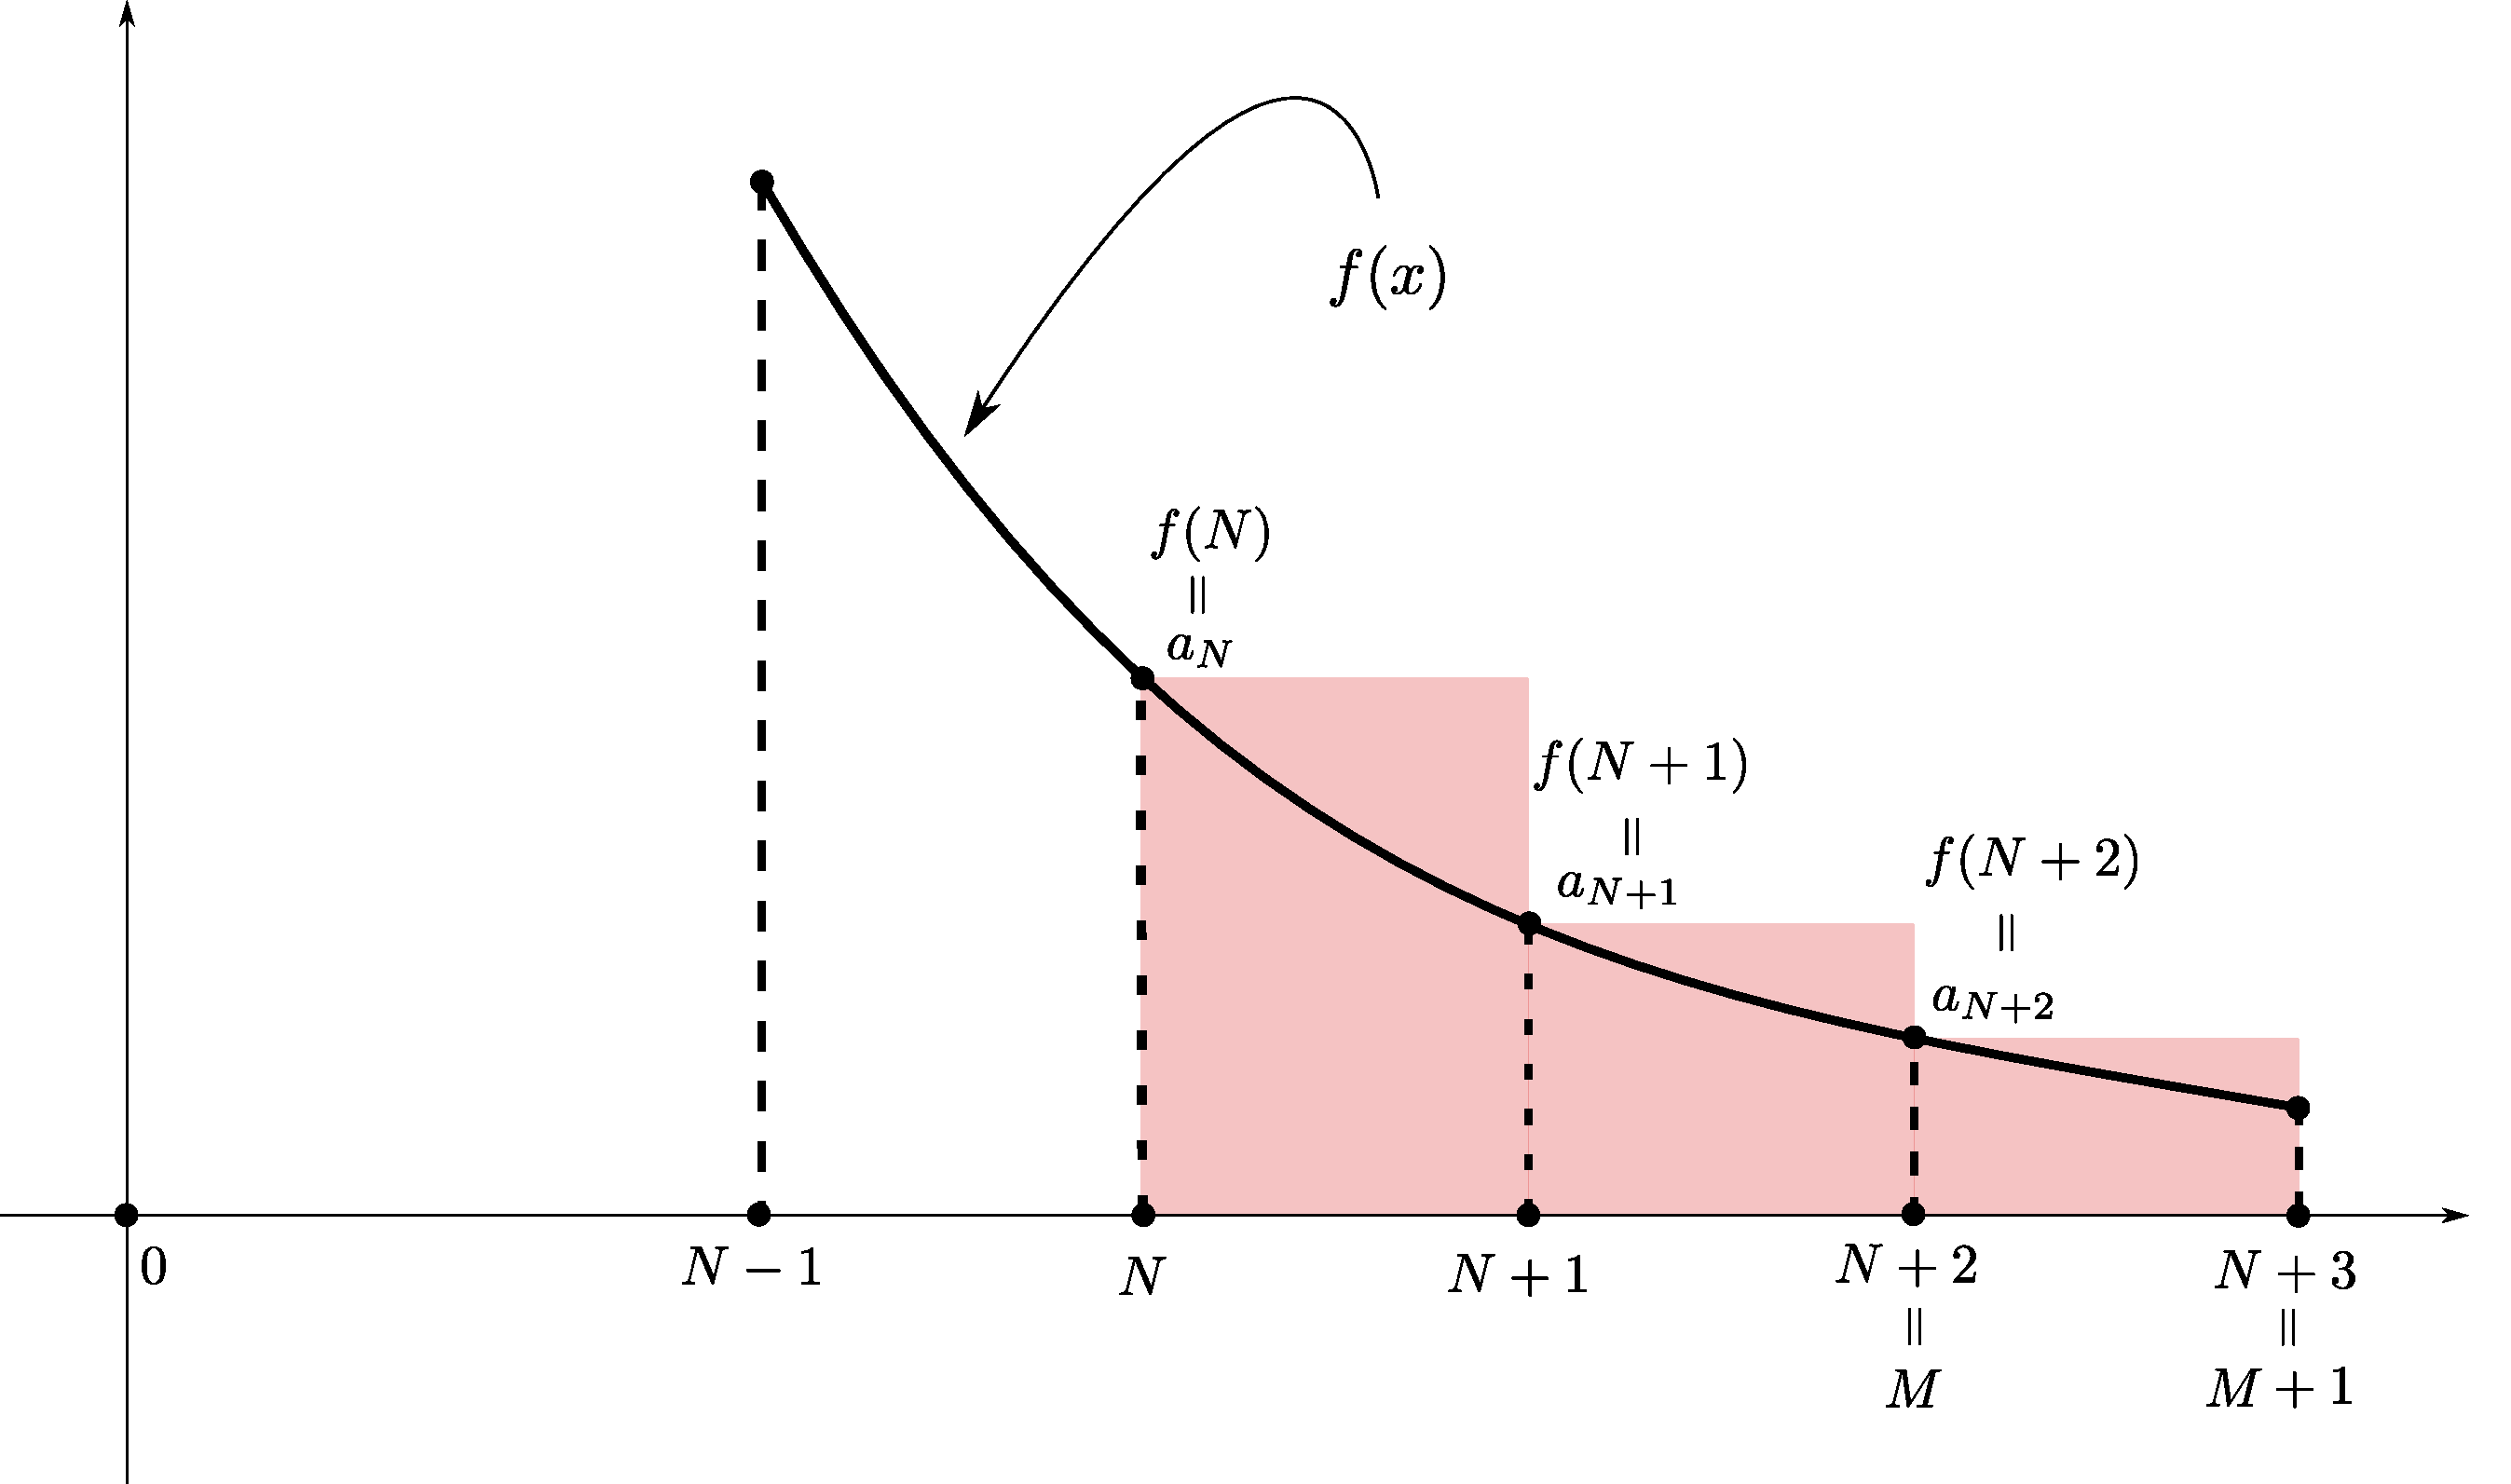
\includegraphics[width=0.63\linewidth]{Figuras/teste-integral-redimensionado1}
\caption{A área hachurada corresponde a soma $\sum_{n=N}^{M}a_n$. Observe que 
o valor desta soma é maior que a integral $\int_{N}^{M+1}f(x)\, dx$.}
\label{fig:teste-integral-redimensionado1}
\end{figure}

Para obter a segunda desigualdade raciocinamos de maneira análoga (bastando apenas
deslocar os retângulo que aparecem na figura acima para esquerda) como mostra
a Figura \ref{fig:teste-integral-redimensionado2}
\begin{figure}[H]
\centering
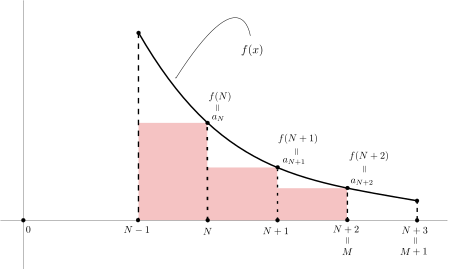
\includegraphics[width=0.63\linewidth]{Figuras/teste-integral-redimensionado2}
\caption{A área hachurada corresponde novamente a soma $\sum_{n=N}^{M}a_n$. Ela é
obtida simplesmente deslocando os retângulos da figura anterior para a esquerda. 
Observe que agora o valor desta soma é menor que a integral $\int_{N-1}^{M}f(x)\, dx$.}
\label{fig:teste-integral-redimensionado2}
\end{figure}
  
  

\end{proof}




\begin{corolario}\label{cor-crit-conv-p-series}
Fixado $p\in [0,+\infty)$, então temos que a $p$-série 
\[
\sum_{n=1}^{\infty} \frac{1}{n^p}
\] 
converge se $p>1$ e diverge se $0\leqslant p\leqslant 1$.
\end{corolario}

\begin{proof}
A prova deste corolário seguirá de uma aplicação do Teste da Integral
(Teorema \ref{teo-teste-da-integral}). Para isto vamos ter que apresentar 
a função $f$, a sequência $(a_n)_{n\in\mathbb{N}\cup\{0\}}$ e 
mostrar que todas as hipóteses do Teorema \ref{teo-teste-da-integral}
são satisfeitas. 

\medskip 
Para isto, podemos tomar $N=2$,
consideramos a sequência $(a_n)_{n\in\mathbb{N}\cup\{0\}}$ dada por $a_0=1$ e 
$a_n=n^{-p}$, para todo $n\in\mathbb{N}$. A função $f:[1,+\infty)\to\mathbb{R}$ 
é escolhida como sendo a função definida por
\[
f(x) = \frac{1}{x^p}.
\]

É imediato verificar que $f$ é monótona não-crescente (note que
$f'(x)<0,\ \forall x\in(1,\infty)$) e que $f(n) = n^{-p}$, para todo $n\in\mathbb{N}$.
Além do mais para todo $M>1$ temos que $f$ é integrável em $[1,M]$ e 
esta integral pode ser explicitamente calculada usando do Teorema Fundamental do Cálculo
como segue. 

Para $p$ positivo e  $p\neq 1$ temos:
\begin{align}\label{eq-aux1-p-series}
\int_{1}^{M}f(x)\, dx
&=
\int_{1}^{M}\frac{1}{x^p}\, dx
=
\int_{1}^{M}x^{-p}\, dx
=
\frac{1}{-p+1} x^{-p+1}\Big|_{1}^{M}
=
\frac{1}{1-p} x^{1-p}\Big|_{1}^{M}
\nonumber
\\[0.3cm]
&=
\frac{M^{1-p}-1}{1-p}
\end{align}

Para $p=1$ temos 
\begin{align}\label{eq-aux2-p-series}
\int_{1}^{M}f(x)\, dx
=
\int_{1}^{M}\frac{1}{x}\, dx
=
\ln(M)-\ln(1)= \ln(M).
\end{align}


Das igualdades \eqref{eq-aux1-p-series} e \eqref{eq-aux2-p-series}
temos que
\begin{align*}
\int_{1}^{\infty} \frac{1}{x^p}\, dx
=
\lim_{M\to\infty} \int_{1}^{M} \frac{1}{x^p}\, dx
&=
\begin{cases}
\displaystyle
\lim_{M\to\infty} \frac{M^{1-p}-1}{1-p},&\ \text{se}\ 0\leqslant p<1;
\\[0.5cm]
\displaystyle
\lim_{M\to\infty} \ln(M),&\ \text{se}\  p=1;
\\[0.5cm]
\displaystyle
\lim_{M\to\infty} \frac{M^{1-p}-1}{1-p},&\ \text{se}\ 1< p<+\infty;
\end{cases}
\\[0.5cm]
&=
\begin{cases}
\displaystyle
+\infty,&\ \text{se}\ 0\leqslant p<1;
\\[0.2cm]
\displaystyle
+\infty,&\ \text{se}\ 0\leqslant p=1;
\\[0.2cm]
\displaystyle
\frac{1}{p-1},&\ \text{se}\ 1< p<+\infty.
\end{cases}
\end{align*}

Finalmente, a prova segue das três igualdades acima e do Teste da Integral.
\end{proof}


\bigskip 
A seguir, lembramos outro importante critério, cuja a contra-positiva se constitui 
em um excelente dispositivo para avaliar se uma série diverge.


\begin{proposicao}\label{prop-conv-term-geral-vai-zero}
Seja $\sum_{n=0}^{\infty} a_n$ uma série de números complexos. 
Se $\sum_{n=0}^{\infty}a_n$ converge, então $a_n\to 0$, quando $n\to\infty$.
\end{proposicao}

\begin{proof}
Já que $\sum_{n=0}^{\infty} a_n$ converge, então sua sequência de somas parciais
forma uma sequência de Cauchy e portanto 
\[
\lim_{n\to\infty} |a_n| = \lim_{n\to\infty} |s_{n+1}-s_n| = 0.
\]
\end{proof}

Uma consequência deste resultado é que se $\sum_{n=0}^{\infty}a_n$
converge, então $(a_n)_{n\in\mathbb{N}\cup\{0\}}$ é uma sequência limitada.

Como veremos na próxima proposição uma 
forma conveniente de estudar a convergência de uma série de números complexos é 
via a série associada dos valores absolutos. Como no caso de séries de números 
reais, esta técnica não se aplica a todos os casos, mas ela é particularmente 
bastante poderosa, pois permite aplicarmos os testes de comparações para 
séries de números não-negativos.


\begin{definicao}
\label{def-conv-absoluta}
\index{Séries!absolutamente convergentes}
Dizemos que $\sum_{n=0}^{\infty} z_n$ converge absolutamente se a série 
$\sum_{n=0}^{\infty}|z_n|$ converge. 
\end{definicao}

\begin{proposicao}\label{prop-conv-abs-implica-conv}
Se a série $\sum_{n=0}^{\infty} z_n$ converge absolutamente, então 
ela é convergente.
\end{proposicao}


\begin{proof}
A ideia da prova consiste novamente em aplicar o critério de Cauchy.
Considere a sequência $(s_n)_{n\in\mathbb{N}\cup\{0\}}$ 
das somas parciais de $(z_n)_{n\in\mathbb{N}\cup\{0\}}$.
Como estamos assumindo que $\sum_{n=0}^{\infty} |z_n|$ converge, 
sabemos que dado $\varepsilon>0$ existe $n_0\in\mathbb{N}$ tal que 
se $m \geqslant n\geqslant n_0$ então 
\[
\Big| |z_n|+|z_{n+1}| +\ldots +|z_m|  \Big|<\varepsilon.
\]
Usando a Desigualdade Triangular e a desigualdade acima, temos
então para todo $m\geqslant n \geqslant n_0$
\begin{align*}
|s_{m}-s_n| = |z_{n}+z_{n+1}+\ldots+ z_{m}|
\leqslant  
\Big| |z_n|+|z_{n+1}| +\ldots +|z_m|  \Big|<\varepsilon.
\end{align*}
Como $\varepsilon>0$ é arbitrário, 
temos que $(s_n)_{n\in\mathbb{N}\cup\{0\}}$ é de Cauchy e portanto 
$\sum_{n=0}^{\infty} z_n$ converge.
\end{proof}


\bigskip 

Um dos exemplos mais importantes de séries que conhecemos é o das 
\textbf{séries geométricas}.
\index{Séries!geometricas}
Esta séries são definidas pelos termos de uma progressão geométrica e desempenham
papel fundamental, por exemplo, no estudo de séries de potências, como veremos adiante.
Esta séries são definidas a partir de uma sequência dada por $a_n = r^n$, 
para todo $n\in\mathbb{N}\cup\{0\}$, onde $r$ é um número real positivo.
Neste caso a sequência das somas parciais de $(a_n)_{n\in\mathbb{N}\cup\{0\}}$
é dada por 
\[
s_n = 1+r+r^2+\ldots r^{n-1}+r^n.
\]
Se $r\neq 1$ sabemos que 
\[
s_n = 1+r+r^2+\ldots r^{n-1}+r^n = \frac{1-r^{n+1}}{1-r}.
\]
Já que temos uma expressão explícita para $s_n$ 
é simples analisar a convergência ou divergência de tais séries. Bastando 
analisar se o limite, quando $n\to\infty$, do lado direito da igualdade acima
existe. E neste caso, se $0<r<1$ temos que $r^{n+1}\to 0$, quando $n\to\infty$,
e consequentemente
\[
\lim_{n\to\infty} s_n
=
\lim_{n\to\infty} \frac{1-r^{n+1}}{1-r}
= 
\frac{\displaystyle\lim_{n\to\infty} (1-r^{n+1})}{1-r} 
=
\frac{1}{1-r}.
\]

Por outro lado, se $r>1$ então temos que $r^{n+1}\to +\infty$, quando $n\to\infty$. 
Portanto
\[
\lim_{n\to\infty} s_n
=
\lim_{n\to\infty} \frac{1-r^{n+1}}{1-r}
= 
\frac{\displaystyle\lim_{n\to\infty} (1-r^{n+1})}{1-r} 
=
+\infty.
\]
No caso em que $r=1$, temos que 
\[
s_n = 1+1^1+1^2+\ldots+1^{n-1}+1^{n}=n+1 \xrightarrow{\ n\to\infty\ } +\infty.
\]


Em resumo, uma série geométrica $\sum_{n=0}^{\infty}r^n$, 
de termos positivos converge se, e somente se,
sua razão $r$ é estritamente menor do que um. 


\bigskip

Já que séries são definidas em termos de sequências de somas parciais. Algumas 
propriedades de sequências são herdadas pelas séries. Abaixo relacionamos alguns
deste fatos simples, mas que serão muito úteis a frente.

\begin{proposicao}
Sejam $\sum_{n=0}^{\infty}z_n$ e $\sum_{n=0}^{\infty}w_n$ duas séries convergentes.
Suponha que $\sum_{n=0}^{\infty}z_n = \alpha$ e $\sum_{n=0}^{\infty} w_n =\beta$.
Então  
\begin{itemize}
	\item a série $\sum_{n=0}^{\infty} cz_n$ converge para $c\alpha$,
	qualquer que seja $c\in\mathbb{C}$;
	
	\item a série $\sum_{n=0}^{\infty}(z_n +w_n)$ converge para $\alpha+\beta$.
\end{itemize}
\end{proposicao}

\begin{proof}
Para cada $n\in\mathbb{N}$, seja $s_n = z_0+z_1+\ldots z_n$, a $n$-ésima soma 
parcial da série $\sum_{n=0}^{\infty} z_n$. Note que, segue 
diretamente das propriedades
algébricas básicas de números complexos que 
a $n$-ésima soma parcial da série $\sum_{n=0}^{\infty} cz_n$ satisfaz a seguinte
igualdade $cz_1+cz_2+\ldots cz_n = cs_n$. Portanto 
\[
\sum_{n=0}^{\infty} cz_n
=
\lim_{n\to\infty} [cz_1+cz_2+\ldots+cz_n]
=
\lim_{n\to\infty} cs_n
=
c\lim_{n\to\infty} s_n
=
c\sum_{n=0}^{\infty} z_n
=
c\alpha.
\]
O que prova a validade do primeiro item da proposição. 

A prova do segundo é no mesmo espírito. Mantendo a notação do item anterior, 
seja $s_n$ a $n$-ésima soma parcial da série $\sum_{n=0}^{\infty}z_n$.
Defina $\widetilde{s}_n$ como sendo a $n$-ésima soma parcial da série
$\sum_{n=0}^{\infty}w_n$. Então, por definição, a $n$-ésima soma parcial da série
$\sum_{n=0}^{\infty}(z_n+w_n)$ satisfaz a seguinte igualdade
\[
(z_0+w_0)+(z_1+w_1)+\ldots+(z_n+w_n) = s_n+\widetilde{s}_n.
\]
Já que a soma de duas sequências convergentes é uma sequência convergente 
e o limite da soma é a soma dos limites, temos que 
a $n$-ésima soma parcial de $\sum_{n=0}^{\infty}(z_n+w_n)$ converge,
quando $n\to\infty$, e além do mais 
\begin{align*}
\sum_{n=0}^{\infty}(z_n+w_n)
&=
\lim_{n\to\infty}
\Big[ (z_0+w_0)+(z_1+w_1)+\ldots+(z_n+w_n) \Big]
\\
&= 
\lim_{n\to\infty}
(s_n+\widetilde{s}_n)
\\
&=
\lim_{n\to\infty}
s_n
+
\lim_{n\to\infty}
\widetilde{s}_n
=
\sum_{n=0}^{\infty}z_n + \sum_{n=0}^{\infty} w_n 
=
\alpha+\beta.
\end{align*}
O que finaliza a prova da proposição.
\end{proof}


\section{Sequências de Funções e Convergência}

Nesta seção vamos definir a noção de sequência de funções, um conceito que
generaliza o conceito de sequências numéricas. Em seguida, vamos discutir
alguns dos conceitos de convergência de sequências de funções. O objetivo
dos conceitos e dos resultados apresentados nesta seção é fornecer um 
arcabouço teórico para estudarmos séries de potencias no plano complexo. 

Diferentemente de sequências de números complexos ou reais, onde
temos um único conceito de convergência, quando
estamos tratando de sequência de funções, há diversas maneiras 
(com características bastante distintas, nem sempre sendo possível 
hierarquizá-las no sentido de apontar qual é a ``melhor'' delas) de 
se definir convergência. Nesta seção vamos apresentar discutir 
sobre três noções de convergência para sequência de funções:
\begin{itemize}
	\item convergência pontual; 
	\item convergência uniforme;
	\item convergência uniforme nas partes compactas.
\end{itemize}

A noção de convergência pontual, como veremos a seguir, é mais simples de 
ser apresentada e de se trabalhar. Por outro lado, a função limite 
obtida por convergência pontual pode não herdar propriedades que
os elementos da sequência de funções possui. Por exemplo, o limite pontual
de uma sequência de funções contínuas pode não ser uma função contínua
(Exemplo \ref{ex-lim-Somas-desc}). 
Ou seja,
é possível construir uma sequência de funções, onde cada elemento desta sequência é 
uma função contínua. Porém a função obtida como limite pontual desta sequência, 
não herda a propriedade de continuidade. Isto alerta para o fato de
que, apesar de ser muito importante e poderosa, a convergência pontual 
pode não ser capaz de fornecer várias informações que eventualmente estaríamos
interessados. 

Para evitar algumas dificuldades técnicas, oriundas do conceito de convergência pontual,
vamos introduzir um outro conceito de convergência de sequência de funções. O conceito de 
convergência uniforme. Embora, seja mais difícil trabalhar com 
este conceito, temos a vantagem de que 
quando conseguimos provar que uma determinada 
sequência de funções converge uniformemente para alguma função complexa, 
então seremos capazes de extrair muito 
mais informações sobre esta função limite! 
Como já deve estar suspeitando o leitor, em geral, não será simples
nem viável provar que uma determinada sequência de funções converge uniformemente 
para uma função limite. Mas em muito casos interessantes será possível mostrar
que se restringimos a nossa sequência de funções, à subconjuntos compactos do
seu domínio, a tarefa de mostrar a convergência uniforme 
poderá ser realizada. A grande vantagem desta abordagem é que mesmo sendo 
este conceito de convergência um pouco mais fraco do que o conceito de convergência
uniforme seremos capazes de mostrar que a função limite preserva diversas propriedades
das ``funções aproximantes''. 
 

O principal exemplo de sequência de funções que o leitor deve ter em mente,
quando estiver lendo esta seção, é o da sequência dos polinômios de 
Taylor de uma série de potências. Vamos estudar
em detalhes esta importante classe de exemplos na Seção \ref{ex-lim-Somas-desc}.


\bigskip 

Em toda esta seção $U\subset\mathbb{C}$ denotará sempre um  
conjunto aberto, que pode ser limitado ou ilimitado. Não há necessidade 
também de assumir que $U$ seja conexo. Isto é, os resultados a serem 
apresentados nesta seção valem para o caso em que $U$ é desconexo. 

\begin{definicao}[Sequência de Funções Complexas]
Dizemos que $(f_n)_{n\in\mathbb{N}\cup\{0\}}$ 
é uma sequência de funções complexas, definidas em $U$, se
\index{Sequência!de funções complexas}
para cada $n\in\mathbb{N}\cup\{0\}$ o termo $f_n$ denota uma 
função definida em $U$ e tomando valores complexos, isto é,  
$f_n:U\to\mathbb{C}$ é uma função.
\end{definicao}

Uma observação importante sobre a definição acima é que em uma sequência
de funções $(f_n)_{n\in\mathbb{N}\cup\{0\}}$ todas as funções da sequência 
estão definidas no mesmo domínio, que aqui convencionamos como sendo um conjunto 
$U\subset \mathbb{C}$ aberto. 

\begin{exemplo}\label{exemplo-seq-func-disco}
Seja $U=\mathbb{D}\subset\mathbb{C}$ o disco unitário. Para cada $n\in\mathbb{N}\cup\{0\}$
seja $f_n:\mathbb{D}\to\mathbb{C}$ a função dada por
\[
f_n(z) = z^n, \qquad \forall\, z\in\mathbb{D}.
\]
Então $(f_n)_{n\in\mathbb{N}\cup\{0\}}$ define uma sequência de funções complexas 
em $\mathbb{D}$.
\end{exemplo}

Sempre que estivermos tratando de sequência de funções é importante deixar claro 
qual é domínio onde as funções da nossa sequência estão definidas. A rigor, a
sequência definida no próximo exemplo é completamente distinta (apesar de sua aparência)
daquela do exemplo anterior

\begin{exemplo}\label{exemplo-seq-func-plano}
Seja $U=\mathbb{C}$. Para cada $n\in\mathbb{N}\cup\{0\}$
seja $g_n:\mathbb{C}\to\mathbb{C}$ a função dada por
\[
g_n(z) = z^n, \qquad \forall\, z\in\mathbb{C }.
\]
Então $(g_n)_{n\in\mathbb{N}\cup\{0\}}$ define uma sequência de funções complexas 
em $\mathbb{C}$.
\end{exemplo}

Apesar da semelhança das leis de $f_n$ e $g_n$, 
apresentadas nos dois exemplos anteriores, 
estas funções devem ser reconhecidas como funções distintas, 
pois possuem domínios distintos. 
Obviamente, $f_n$ pode ser vista 
como a restrição de $g_n$ ao disco unitário. Mas o leitor deve estar atento
que a rigor $f_n$ e $g_n$ devem ser tratadas como funções distintas.
A importância de se fazer tal distinção ficará ainda mais clara, quando introduzirmos 
os conceitos de convergência. Por exemplo, veremos, a frente, que a sequência 
$(f_n)_{n\in\mathbb{N}\cup\{0\}}$ será convergente (no sentido da convergência pontual - a ser definida), porém a sequência $(g_n)_{n\in\mathbb{N}\cup\{0\}}$ não será pontualmente convergente!


\begin{exemplo}
Sejam $U=\mathbb{D}\subset\mathbb{C}$ o disco unitário e 
$(f_n)_{n\in\mathbb{N}\cup\{0\}}$ a sequência de funções 
definidas no Exemplo \ref{exemplo-seq-func-disco}.
Para cada $n\in\mathbb{N}\cup\{0\}$
defina a função $S_n:\mathbb{D}\to\mathbb{C}$ como sendo
\[
S_n(z) = 1+z+z^2+\ldots+z^n = \sum_{j=0}^{n} f_n(z), \qquad \forall\, z\in\mathbb{D}.
\]
Então $(S_n)_{n\in\mathbb{N}\cup\{0\}}$ define uma sequência de funções complexas 
em $\mathbb{D}$. O leitor pode observar que esta sequência de funções é o análogo, 
para sequência de funções, do conceito de sequência de somas parciais. 
Além do mais, para cada $z\in\mathbb{D}$ fixado a sequência numérica
$(S_n(z))_{n\in\mathbb{N}\cup\{0\}}$ representa 
as somas parciais de uma série geométrica de razão $z$. 
\end{exemplo}



\begin{definicao}[Sequência de Somas Parciais de uma sequência de funções]
\label{def-seq-somasparciais-funcoes}
Seja $(f_n)_{n\in\mathbb{N}\cup\{0\}}$ uma sequência de funções complexas 
definida em $U$. Definimos a sequência das somas parciais
de $(f_n)_{n\in\mathbb{N}\cup\{0\}}$, como sendo uma nova sequência de funções 
complexas $(S_n)_{n\in\mathbb{N}\cup\{0\}}$ definidas em $U$, onde 
para cada $n\in\mathbb{N}\cup\{0\}$, a função $S_n:U\to\mathbb{C}$ é dada por 
\[
S_n(z) = f_0(z)+f_1(z)+f_2(z)+\ldots+f_n(z) = \sum_{j=0}^n f_j(z),
\qquad \forall z\in U.
\]
\end{definicao}


Os exemplos que devem aparecer com mais frequência neste texto relacionados
a sequências de funções e suas respectivas sequências de somas parciais são
os seguintes: 

\begin{exemplo}\label{exe-seq-fun-series-pot}
Dada uma sequência numérica $(a_n)_{n\in\mathbb{N}\cup\{0\}}$ arbitrária 
de números complexos e um aberto $U\subset\mathbb{C}$, 
defina a seguinte sequência de funções complexas 
$(f_n)_{n\in\mathbb{N}\cup\{0\}}$, onde para cada $n\in\mathbb{N}$, 
a função $f_n:U\to\mathbb{C}$ é dada por
\[
f_n(z) = a_nz^n, \qquad \forall z\in U.
\] 

Então a sequência das somas parciais de $(f_n)_{n\in\mathbb{N}\cup\{0\}}$,
denotada por $(S_n)_{n\in\mathbb{N}\cup\{0\}}$ é dada por 
\[
S_n(z) = a_0+a_1z+a_2z^2+\ldots +a_{n-1}z^{n-1}+a_nz^n = \sum_{j=0}^n a_jz^j, 
\qquad \forall z\in U.
\]
\end{exemplo}



\begin{exemplo}\label{ex-somas-parciais-zeta}
Seja $U=\{z\in\mathbb{C}: \Re(z)>1\}$ e $\log:\mathbb{C}\setminus L_{\pi}\to\mathbb{C}$
o ramo principal do logaritmo.
Seja $(f_n)_{n\in\mathbb{N}}$ a sequência de funções complexas, onde para cada 
$n\in\mathbb{N}$, a função $f_n:U\to\mathbb{C}$ é definida por
\[
f_n(z) = \exp(-z\log n) = \frac{1}{\exp(z\log n)} = \frac{1}{n^z}.
\]
Então $(S_n)_{n\in\mathbb{N}}$, a sequência das somas parciais de $(f_n)_{n\in\mathbb{N}}$ é 
dada por
\[
S_n(z) = 1+\frac{1}{2^z}+\ldots+\frac{1}{n^z} = \sum_{j=1}^n \frac{1}{j^z}.
\]
\end{exemplo}



\begin{definicao}[Convergência Pontual]
\index{Convergência!pontual}
Sejam $U\subset\mathbb{C}$ um conjunto aberto e $(f_n)_{n\in\mathbb{N}\cup\{0\}}$
uma sequência de funções complexas definidas em $U$. Dizemos que a sequência de
funções $(f_n)_{n\in\mathbb{N}\cup\{0\}}$ \textbf{converge pontualmente} para uma função complexa $f:U\to\mathbb{C}$ se para cada $z\in U$ temos 
\[
\lim_{n\to\infty} f_n(z) = f(z).
\]
\end{definicao}


Do ponto de vista da definição forma de limite a noção de convergência pontual
pode ser reformulada da seguinte forma. 
Seja $(f_n)_{n\in\mathbb{N}\cup\{0\}}$ uma sequência de funções complexas
definidas em $U$ que converge pontualmente para $f:U\to\mathbb{C}$. Então podemos
afirmar que dado $\varepsilon>0$ e fixado $z\in U$, 
existe $n_0\equiv n_0(z,\varepsilon)\in\mathbb{N}$
tal que se $n\geqslant n_0$ então 
\[
|f_n(z)-f(z)|<\varepsilon.
\]
Isto quer dizer que, fixado $\varepsilon>0$ então 
a imagem de $z$ por $f$ está $\varepsilon$-próxima da 
imagem de $z$ por $f_n$, sempre que $n$ for maior ou igual a 
$n_0(\varepsilon,z)$ que pode depender de $\varepsilon$ e eventualmente 
também de $z$.
Observe que não há nenhum conflito, com a observação acima, em dizer que existe 
$w\in U$ tal que 
\[
|f_{n_0(\varepsilon,z)}(w)-f(w)| \geqslant \varepsilon 
\]

\begin{figure}[H]
\centering
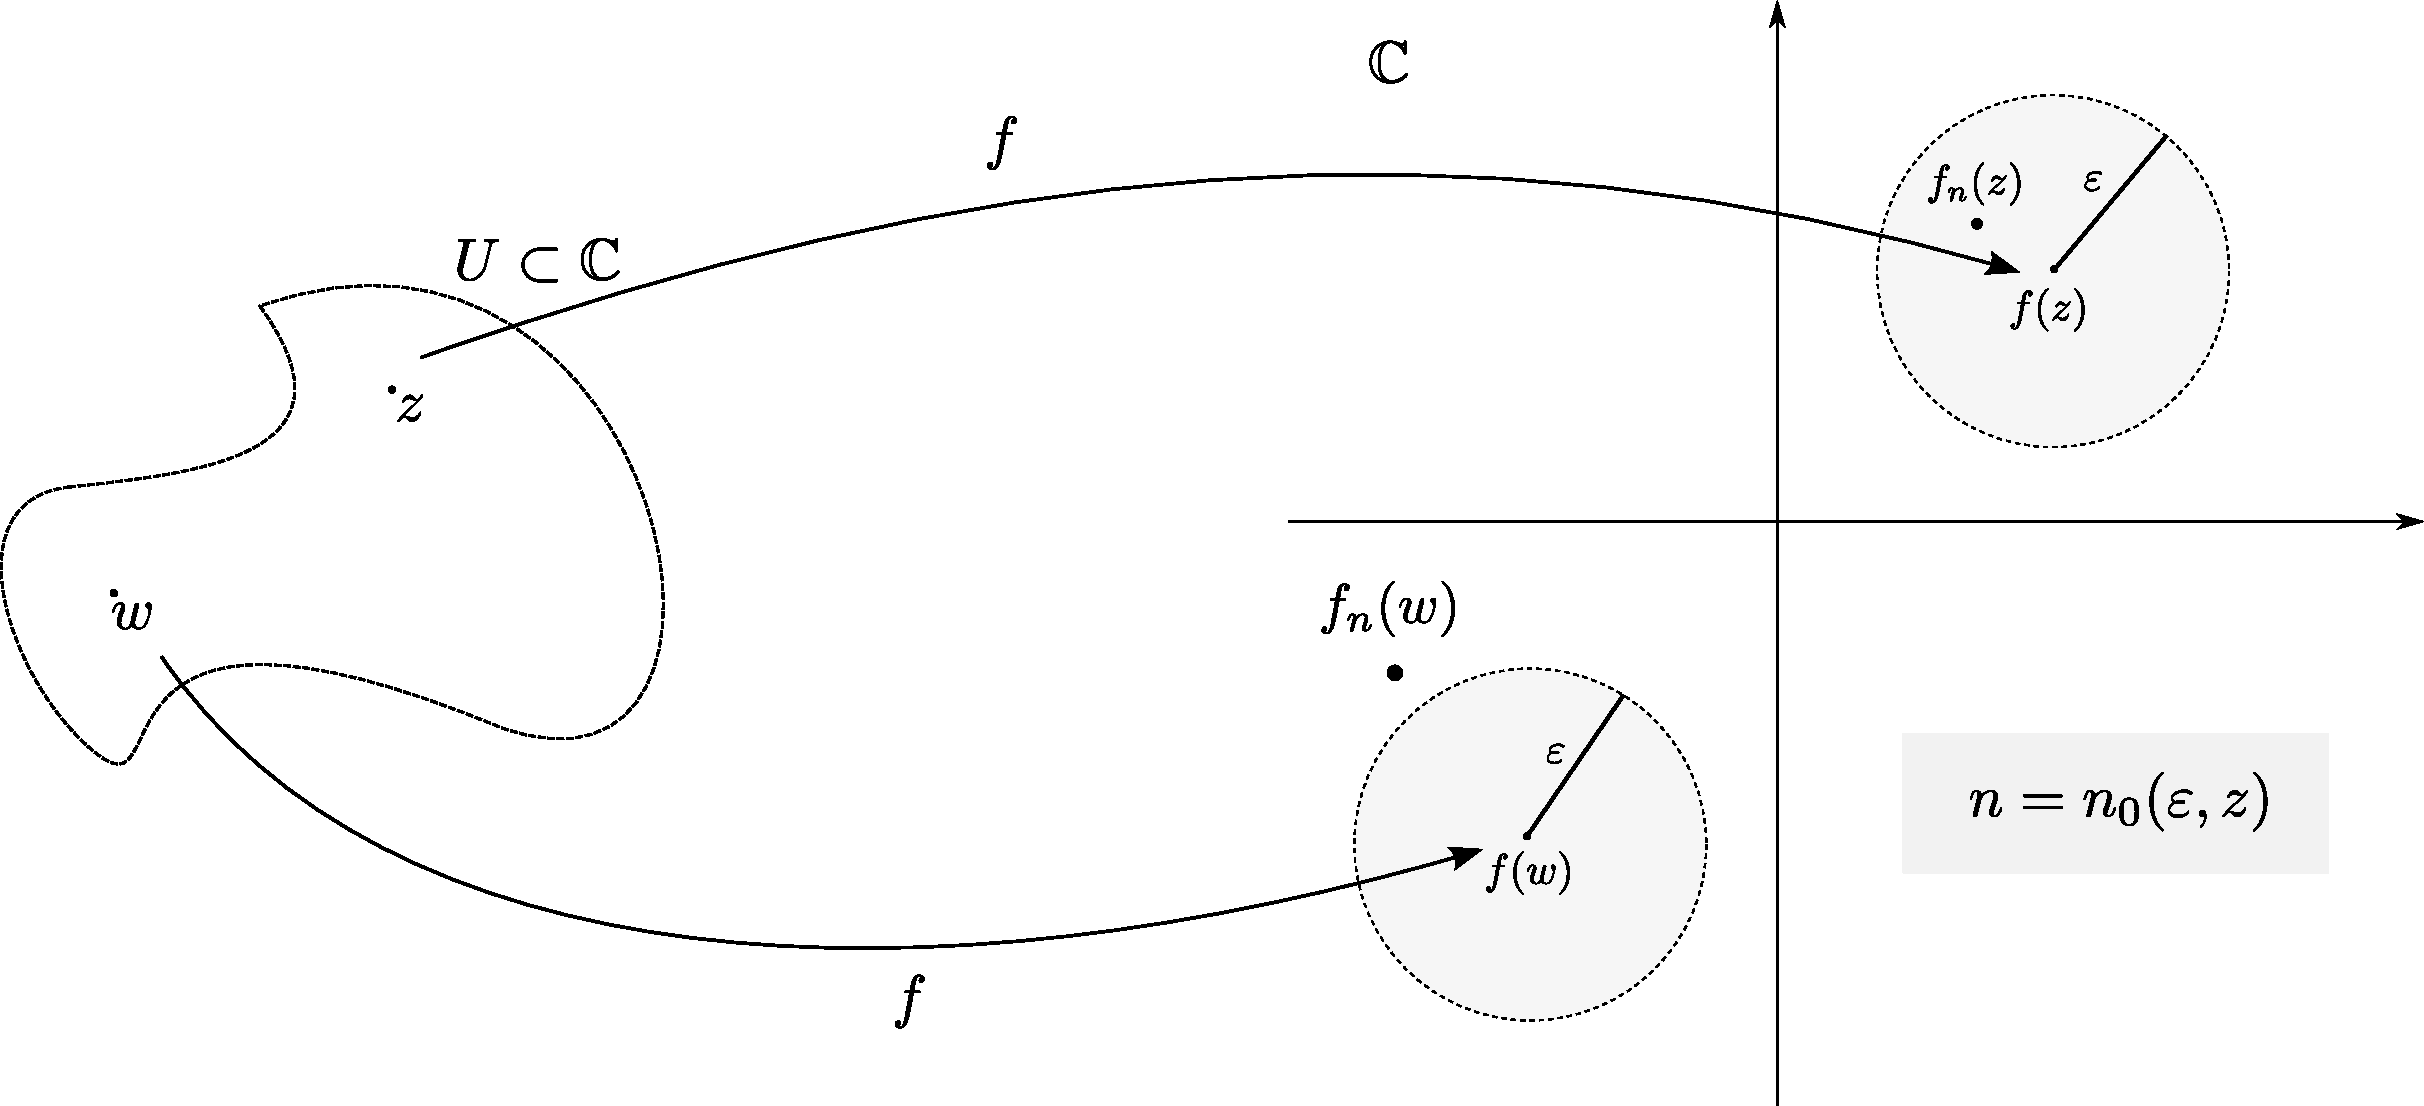
\includegraphics[width=0.95\linewidth]{Figuras/convergencia-pontual-redimensionado}
\caption{Na figura acima, temos uma sequência de funções 
$(f_n)_{n\in\mathbb{N}\cup\{0\}}$ converge pontualmente para $f$. 
Mas note que pode acontecer da convergência ser mais ``lenta'' para alguns pontos. Nesta
figura vimos que $f_n(z)$ está $\varepsilon$ próximo de $f(z)$ mas o mesmo não ocorre
para $f_n(w)$. Como sabemos que $f_n(w)$ converge para $f(w)$ o que está acontecendo
nesta situação é que é necessário tomar o índice $n$ em $f_n(w)$ muito maior do 
que $n_0(\varepsilon,z)$.}
\label{fig:convergencia-pontual-redimensionado}
\end{figure}


A desigualdade acima poderia ser válida inclusive para uma quantidade finita 
de índices consecutivos a $n_0(\varepsilon,z)$, isto é, para 
$n_0(\varepsilon,z)+k$, com $k\in\{1,\ldots,m\}$, ou seja, poderíamos ter ainda
\[
|f_{n_0(\varepsilon,z)+k}(w)-f(w)| \geqslant \varepsilon,
\qquad k\in\{1,\ldots,m\}. 
\] 
Mas é claro, como a propriedade que define a convergência pontual exige que
\[
\lim_{n\to\infty} f_n(w) = f(w),
\]
e por isto, sabemos que deverá existir algum natural $n_1(\varepsilon,w)>n_0(\varepsilon,z)$ (que poderia talvez ser muito maior que $n_0(\varepsilon,z)$) 
satisfazendo
\[
|f_{n}(w)-f(w)| < \varepsilon, \qquad \forall n\geqslant n_1(\varepsilon,w).
\]

Se $(f_n)_{n\in\mathbb{N}\cup\{0\}}$ é uma sequência de funções complexas definidas em
$U$ que converge pontualmente para $f:U\to\mathbb{C}$, então é comum às vezes 
nos referirmos a $f_n$ como uma aproximante de $f$.


\bigskip 
Vamos analisar se as sequências $(f_n)_{n\in\mathbb{N}\cup\{0\}}$ 
e $(g_n)_{n\in\mathbb{N}\cup\{0\}}$ dos Exemplos \ref{exemplo-seq-func-disco}
e \ref{exemplo-seq-func-plano} e verificar se elas convergem pontualmente para alguma função.


Vamos considerar primeiro a sequência de funções do Exemplo \ref{exemplo-seq-func-disco}.
Neste caso, $U=\mathbb{D}$ e para cada $n\in\mathbb{N}$ temos que 
$f_n:\mathbb{D}\to\mathbb{C}$ é dada por $f_n(z)=z^n$. Como qualquer ponto $z\in\mathbb{D}$
pode ser representado em coordenadas polares na forma $z=re^{i\theta}$, onde $0\leqslant r< 1$
e $\theta\in [0,2\pi)$ temos que 
\[
\lim_{n\to\infty} f_n(z) 
= 
\lim_{n\to\infty} z^n 
=
\lim_{n\to\infty} (re^{i\theta})^n
=
\lim_{n\to\infty}r^n e^{in\theta}=0.
\]
Como $z\in\mathbb{D}$ é arbitrário então temos que $(f_n)_{n\in\mathbb{N}\cup\{0\}}$ 
converge pontualmente para a função identicamente nula em $U$, isto é, 
$f:U\to\mathbb{C}$ dada por $f(z)=0$ para todo $z\in\mathbb{D}$.

Por outro lado, podemos ver que a sequência apresentada no Exemplo 
\ref{exemplo-seq-func-plano} não converge pontualmente para nenhuma função 
complexa. De fato, basta observar que existe um ponto 
(na verdade, poderíamos tomar qualquer ponto no conjunto $\mathbb{C}\setminus (\mathbb{D}\setminus\{1\})$) $z\in \mathbb{C}$ para o qual $g_n(z)$ não converge. Por exemplo, tome 
$z=1+i$. Representando este ponto em coordenadas polares, $z=\sqrt{2}e^{i\pi/4}$,
podemos calcular facilmente $z^n = 2^{n/2}e^{in\pi/4}$. 
Já que $|z^n|=2^{n/2}\xrightarrow{\ n\to\infty\ }+\infty$,
segue que $g_n(z)=z^n$ não converge. Portanto não existe nenhuma função $f:\mathbb{C}\to\mathbb{C}$
tal que $(g_n)_{n\in\mathbb{N}\cup\{0\}}$ converge pontualmente para $g$.


\medskip 

Vamos analisar agora a convergência das somas 
parciais do Exemplo \ref{ex-somas-parciais-zeta}.
Neste exemplo, a sequência que gera as somas parciais é definida no 
conjunto $\{z\in\mathbb{C}: \Re(z)>1\}$ e dada por $f_n(z)= \exp(-z\ln n) = 1/n^z$
e as somas parciais são dadas por 
\[
S_k(z) = \sum_{n=1}^{k}\frac{1}{n^z}.
\]
Vamos mostrar, para cada $z\in\{z\in\mathbb{C}: \Re(z)>1\}$ 
que  $(S_n)_{n\in\mathbb{N}}$ converge para um função complexa
$\zeta:\{z\in\mathbb{C}: \Re(z)>1\}\to\mathbb{C}$. 

De fato, para cada $n\in\mathbb{N}$ e $z\in\{z\in\mathbb{C}: \Re(z)>1\}$ 
temos
\[
|f_n(z)| = \frac{1}{n^z}  = |\exp(-z\ln n)| = \exp(-\Re(z)\ln n) = \frac{1}{n^{\Re(z)}}.
\]
Pela desigualdade triangular temos a seguinte estimativa 
\[
|S_k(z)| 
\leq 
\sum_{n=1}^{k}\left|\frac{1}{n^z}\right|
=
\sum_{n=1}^{k} \frac{1}{n^{\Re(z)}}.
\]
Note que no lado direito da igualdade acima, temos a $k$-ésima soma parcial
de uma $p$-série, onde $p=\Re(z)$. 
Já que $z\in\{z\in\mathbb{C}: \Re(z)>1\}$ segue do Corolário \ref{cor-crit-conv-p-series} 
que 
\[
\sum_{n=1}^{\infty}\left|\frac{1}{n^z}\right|
=
\sum_{n=1}^{\infty} \frac{1}{n^{\Re(z)}}.
\]
converge. Então segue da Proposição \ref{prop-conv-abs-implica-conv} que a série
abaixo é convergente
\[
\sum_{n=1}^{\infty} f_n(z) \equiv \sum_{n=1}^{\infty} \frac{1}{n^z}
\]
para cada $z\in\{z\in\mathbb{C}: \Re(z)>1\}$. Logo
existe um número complexo que chamaremos de 
$\zeta(z)$ tal que 
\[
\zeta(z) = \sum_{n=1}^{\infty} \frac{1}{n^z}.
\]

A análise acima mostra que podemos associar a cada $z\in\{z\in\mathbb{C}: \Re(z)>1\}$ 
um número complexo $\zeta(z)\in\mathbb{C}$ dado pelo série acima.
Desta forma temos uma função complexa $\zeta:\{z\in\mathbb{C}: \Re(z)>1\}\to\mathbb{C}$
que é o limite pontual da sequência $(S_n)_{n\in\mathbb{N}}$. 
Esta função é chamada de \textbf{função zeta de Riemann}.
\index{Função!zeta de Riemann}
Na verdade, há um pequeno abuso de terminologia, pois a função que de fato é chamada
de função zeta de Riemann é uma função complexa definida no conjunto $\mathbb{C}\setminus\{1\}$
e a função que temos acima, é na verdade a restrição da verdadeira função zeta de Riemann
ao semi-plano $\{z\in\mathbb{C}: \Re(z)>1\}$.
Para não ter perigo de confusão, nesta seção o que vamos chamar 
de função zeta de Riemann é a
função que acabamos de definir acima, e seu domínio é precisamente o 
semi-plano $\{z\in\mathbb{C}: \Re(z)>1\}$.

Como para cada $n\in\mathbb{N}$, temos que 
temos que a função $z\longmapsto S_n(z)$ é contínua e mais ainda holomorfa
na região $\{z\in\mathbb{C}: \Re(z)>1\}$; e obtida como limite pontual de $(S_n)_{n\in\mathbb{N}}$, duas perguntas que surgem naturalmente são:
\begin{itemize}
	\item a função $\zeta:\{z\in\mathbb{C}: \Re(z)>1\}\to\mathbb{C}$ é uma função contínua?  
	\item a função $\zeta:\{z\in\mathbb{C}: \Re(z)>1\}\to\mathbb{C}$ é uma função holomorfa?
\end{itemize}

Na verdade, a resposta para as duas perguntas é positiva. Mas como vamos
ver a seguir, responder estas perguntas vão requerer uma análise um pouco mais
refinada sobre a convergência da sequência $(S_n)_{n\in\mathbb{N}}$.


\begin{exemplo}\label{ex-lim-Somas-desc}
Considere a sequência de funções complexas $(f_n)_{n\in\mathbb{N}\cup\{0\}}$,
onde para cada $n\in\mathbb{N}\cup\{0\}$ a função 
$f_n:\mathbb{C}\to\mathbb{C}$ é dada por 
\begin{align*}
f_n(z) = \frac{|z|^2}{(1+|z|^2)^n}.
\end{align*}
Seja $(S_n)_{n\in\mathbb{N}\cup\{0\}}$ a sequência das somas parciais de $(f_n)_{n\in\mathbb{N}\cup\{0\}}$. 

\medskip 
Vamos mostrar a seguir que $(S_n)_{n\in\mathbb{N}\cup\{0\}}$ converge pontualmente para a função 
$S:\mathbb{C}\to\mathbb{C}$ dada por
\[
S(z) 
=
\begin{cases}
0,&\text{se}\ z=0;\\
1+|z|^2,&\text{se}\ z\neq 0.
\end{cases}
\]
Fornecendo Assim um exemplo de uma sequência 
$(S_n)_{n\in\mathbb{N}\cup\{0\}}$
de funções complexas \textbf{contínuas}
convergindo para uma função complexa descontínua 
(note que a função $S$ não é contínua na origem). 

Vamos então verificar que 
\[
\lim_{n\to\infty} S_n(z) = S(z), \qquad \forall z\in\mathbb{C}.
\]
Para isto vamos considerar separadamente os casos $z=0$ e $z\neq 0$.

No caso $z=0$, temos para todo $n\geqslant 0$ que
\[ 
S_n(0) = \sum_{j=0}^n f_j(0) = 0
\]
Logo $S_n(0)\xrightarrow{\ n\to\infty\ }0=S(0)$.

No caso $z\neq 0$, 
\[ 
S_n(z) 
= \sum_{j=0}^n f_j(z) 
= \sum_{j=0}^n \frac{|z|^2}{(1+|z|^2)^n}
= |z|^2 \sum_{j=0}^n \frac{1}{(1+|z|^2)^n}.
\]
Já  que para cada $z\neq 0$ fixado, temos $(1+|z|^2)>1$, é imediato verificar 
que $S_n(z)$ é a $n$-ésima soma parcial de uma série geométrica de razão 
\[
r = \frac{1}{1+|z|^2}<1.
\]

Portanto podemos obter explicitamente a expressão do limite de $S_n(z)$,
quando $n\to\infty$, como segue
\begin{align*}
\lim_{n\to\infty} S_n(z) 
&=
|z|^2 \lim_{n\to\infty}\sum_{j=0}^n \frac{1}{(1+|z|^2)^j}
=
|z|^2 
\sum_{n=0}^{\infty} r^n
=
|z|^2 \frac{1}{1-r}
\\
&
=
|z|^2 \ \frac{1}{1- \frac{1}{1+|z|^2} }
\\
&=
1+|z|^2.
\\
&=
S(z).
\end{align*}
\end{exemplo}



Em resumo, o exemplo acima mostra que o limite pontual de uma soma 
de funções contínuas pode \textbf{não} ser uma função contínua. Deixando bem claro
que mesmo a questão da continuidade da função zeta Riemann é um fato
não-trivial. Além do mais, questões similares a estas são relevantes e naturais
também no contexto de séries de potências. Na próxima seção 
vamos estudá-las detalhadamente.


\section{Séries de Potências}
\label{sec-series-potencias}

Nesta seção vamos apresentar a definição e estudar algumas propriedades
básicas sobre séries de potências no plano complexo. 

Vamos usar séries de potências para dar importantes exemplos
de funções analíticas. Ao longo da seção o leitor deve notar
que alguns dos resultados apresentados aqui 
se assemelham a outros resultados familiares que aparecem até 
mesmo nos cursos introdutórios de Cálculo. 




\subsection{Séries de Potências Centradas na Origem}
\label{subsec-series-pot-centro-zero}
\begin{definicao}[Séries de Potências]
\label{def-series-de-potencias}
\index{Séries!de potências}
Sejam $(a_n)_{n\in\mathbb{N}\cup\{0\}}$ uma sequência 
de número complexos e $z\in\mathbb{C}$ um número complexo fixado. 
Considere a sequência $(a_nz^n)_{n\in\mathbb{N}\cup\{0\}}$.
A série numérica associada a esta sequência, isto é,
\[
\sum_{n=0}^{\infty} a_n\, z^n,
\]
é chamada série de potências de centro em $0$.
\end{definicao}


Convidamos o leitor a reler, neste momento, 
cuidadosamente a definição de séries 
numéricas (Definição \ref{def-series-num-complexos}).

Ela diz que a série gerada pela sequência
$(a_nz^n)_{n\in\mathbb{N}\cup\{0\}}$ 
como objeto matemático é na verdade outra sequência 
a chamada sequência de somas parciais, que será denotada por $(S_n(z))_{n\in\mathbb{N}\cup\{0\}}$ e dada por

\begin{align*}
S_0(z) 	&= a_0
\\
S_1(z) 	&= a_0+a_1z
\\
S_2(z) 	&= a_0+a_1z+a_2z^2
\\
S_3(z)	&= a_0+a_1z+a_2z^2+a_3z^3
\\
		&\vdots	
\\
S_n(z)	&= a_0+a_1z+a_2z^2+\ldots+a_nz^n
\\
		&\vdots	
\end{align*}

Portanto seguindo a Definição \ref{def-series-num-complexos} dizemos que
a série de potências 
\[
\sum_{n=0}^{\infty} a_n\, z^n,
\]
converge, se a sequência das somas parciais $(S_n(z))_{n\in\mathbb{N}\cup\{0\}}$ 
converge, isto é, 
existe um número complexo, que sugestivamente será chamado de $f(z)$, tal que
\[
\lim_{n\to\infty} S_n(z) = f(z).
\]


Olhando apenas para os pontos $z\in\mathbb{C}$ 
onde $(S_n(z))_{n\in\mathbb{N}\cup\{0\}}$
converge, podemos definir uma função. A função que leva $z$ em 
$\lim_{n\to\infty}S_n(z)=f(z)$.
A função $f$ definida desta maneira tem seu domínio dado precisamente pelo conjunto 
\[
\mathrm{dom}(f) = 
\Big\{ z\in\mathbb{C} :  \ \text{existe} \ \lim_{n\to\infty}S_n(z)  \Big\}.
\]

Apesar de muito simples, esta descrição, do domínio de $f$, 
é de pouca utilidade. Por exemplo, se estivermos interessados
em estudar continuidade ou diferenciabilidade de $f$ 
em um ponto $z_0$ de seu domínio, vamos precisar
saber, além de outras coisas, se $f$ também está bem definida em todos os pontos de algum disco
com centro em $z_0$ e raio positivo. 
Em outras palavras, do ponto de vista mais clássico de
se fazer uma teoria de cálculo, nos interessa mais é saber quem é o interior 
do domínio de $f$, que seguindo a notação da seção sobre topologia no 
plano complexo era denotado por $\mathrm{int}(\mathrm{dom}(f))$.


\medskip 
Observamos que determinar exatamente o domínio da função $f$, dada acima,
pode ser uma tarefa extremamente complicada. 
Por outro lado, provaremos, a seguir, um resultado incrível 
(Teorema \ref{teo-exist-raio-conv})
que afirma que este domínio é ``moralmente'' 
um disco. 
Mais precisamente, vamos demonstrar que existe um único $R\in [0,+\infty]$ tal que
\[
\mathrm{dom}(f)\subset \overline{D(0,R)} 
\qquad \text{e} \qquad 
\mathrm{int}(\mathrm{dom}(f)) = D(0,R),
\]
e além do mais, este número $R$ depende apenas da sequência 
$(a _n)_{n\in\mathbb{N}\cup\{0\}}$ e dado explicitamente por
\[
R 
= 
\begin{cases}
\frac{1}{ \displaystyle\limsup_{n\to\infty} \sqrt[n]{|a_n|} },&
\ \ \text{se}\ \limsup_{n\to\infty} \sqrt[n]{|a_n|}\neq 0;
\\[1.0cm]
+\infty,&\ \ \text{se}\ \limsup_{n\to\infty} \sqrt[n]{|a_n|}=0,
\end{cases}
\]
onde 
\[
\limsup_{n\to\infty} \sqrt[n]{|a_n|}
\equiv 
\lim_{n\to\infty} \left[ \sup \Big\{ \sqrt[n]{|a_n|}, \sqrt[n+1]{|a_{n+1}|}, \sqrt[n+2]{|a_{n+2}|},\ldots  \Big\} \right].
\]

Se $R=0$ então a série de potências só converge na origem. 
Para $R=+\infty$ a série converge para qualquer escolha de $z\in \mathbb{C}$
o que motiva usar a notação $D(0,+\infty)\equiv \mathbb{C}$.


\bigskip 
Do que foi enunciado acima, 
concluímos que o domínio de $f$ é sempre o disco aberto de centro zero 
e raio $R$ unido eventualmente 
com mais alguns pontos do bordo deste disco (a circunferência $\partial D(0,R)$).
Como no caso de séries de potências de números reais, o número $R$ 
é chamado de raio de convergência da série de potencias e $D(0,R)$
o disco de convergência.  

Após feita as provas dos fatos mencionados acima teremos preparado o 
terreno para olhar para séries de potências como limites de sequências
de funções. Antes porém vamos gostaríamos de acrescentar alguns comentários
sobre o raio de convergência. 



\bigskip

À primeira vista a expressão de $R$ pode parecer assustadora, mas
observamos que em vários exemplos práticos, teremos
\[
\limsup_{n\to\infty} \sqrt[n]{|a_n|} = \lim_{n\to\infty} \sqrt[n]{|a_n|}.
\]
Ou seja, o ``limsup'' é simplesmente o limite. 
Na verdade, isto sempre acontece quando o limite existe.
Mas é importantíssimo observar que nem toda sequência da forma $\sqrt[n]{|a_n|}$
possui limite em $[0,+\infty]$. 
Por outro lado, $\limsup_{n\to\infty} \sqrt[n]{|a_n|}$
está sempre bem definido como um ponto em $[0,+\infty]$. 
Portanto é sempre lícito escrever 
\[
\limsup_{n\to\infty} \sqrt[n]{|a_n|},
\]
independentemente de quem é a sequência  $(a_n)_{n\in\mathbb{N}\cup\{0\}}$.
Mas devemos estar atentos ao fato de que nem sempre faz sentido escrever 
\[
\lim_{n\to\infty} \sqrt[n]{|a_n|}.
\]
Os exemplos a seguir, deixam mais claro este comentário.

\bigskip 

Suponha que $(a_nz^n)_{n\in\mathbb{N}\cup\{0\}}$ seja uma sequência dada por 
\[
a_n 
= 
(2\cos(n\pi)+1)^n, 
\ \text{então}\ \ 
\sqrt[n]{|a_n|} 
=  
\cos(n\pi)+2
=
\begin{cases}
3,& \text{se}\ n \ \text{é ímpar}; 
\\
1,& \text{se}\ n \ \text{é par};  
\end{cases}
\]
então $\sqrt[n]{|a_n|}$ oscila entre $3$ e $1$. 
Assim esta sequência não pode convergir, isto é,
\[
\textbf{não existe} \quad \lim_{n\to\infty}\sqrt[n]{|a_n|}.
\]

Por outro lado, como já comentamos, ela necessariamente 
possui limsup e ele é dado por
\begin{align*}
\limsup_{n\to\infty}\sqrt[n]{|a_n|}
&=
\lim_{n\to\infty} 
\left[ \sup \Big\{ \sqrt[n]{|a_n|}, \sqrt[n+1]{|a_{n+1}|}, \sqrt[n+2]{|a_{n+2}|},\ldots  \Big\} \right]
\\
&=
\lim_{n\to\infty} \left[ \sup \Big\{ 2\cos(n\pi)+1,\, 2\cos((n+1)\pi)+1,\ldots  \Big\} \right]
\\
&=
\lim_{n\to\infty} [ \sup \{ 1,3 \} ]
\\
&=
\lim_{n\to\infty} 3 = 3.
\end{align*} 



Outro exemplo importante é dado pela sequência $a_n = n^n(1-\cos(n\pi))^n$.
Neste caso temos
\[
\sqrt[n]{|a_n|} = n(1-\cos(n\pi)) 
= 
\begin{cases}
2n,& \text{se}\ n \ \text{é ímpar}; 
\\
0,& \text{se}\ n \ \text{é par};  
\end{cases}
\]

Novamente vemos que a sequência $\sqrt[n]{|a_n|}$ não tem limite 
pois neste caso, apesar dos termos ímpares ficarem arbitrariamente 
grandes (dando a impressão de que a sequência poderia convergir para $+\infty$) 
os termos pares desta sequência são nulos. 
Logo, entre dois índices consecutivos, 
os termos desta sequências oscilam entre um número grande $2n$ e zero e portanto \textbf{não} converge para $+\infty$, ou seja,
\[
\textbf{não existe} \quad \lim_{n\to\infty}\sqrt[n]{|a_n|}.
\]

Por outro lado, podemos calcular facilmente 
$\limsup_{n\to\infty}\sqrt[n]{|a_n|}$.
Basta observar que para qualquer $n\in\mathbb{N}$ fixado, que como conjunto (eliminando as vezes que o zero se repete e escrevendo seus elementos em ordem crescente) temos
\[
\Big\{ \sqrt[n]{|a_n|}, \sqrt[n+1]{|a_{n+1}|}, \sqrt[n+2]{|a_{n+2}|},\ldots  \Big\}
=
\{0,2,6,10,\ldots\}
\]
e portanto 
\begin{align*}
\limsup_{n\to\infty} \sqrt[n]{|a_n|}
&\equiv 
\lim_{n\to\infty} \left[ \sup \Big\{ \sqrt[n]{|a_n|}, \sqrt[n+1]{|a_{n+1}|}, \sqrt[n+2]{|a_{n+2}|},\ldots  \Big\} \right]
\\
&=
\lim_{n\to\infty}\sup \{0,2,6,10,\ldots\}
\\
&=
\lim_{n\to\infty}+\infty
\\
&=
+\infty.
\end{align*}


Mas como dissemos, há vários casos em que 
$\lim_{n\to\infty} \sqrt[n]{|a_n|}$ existe. 
Nestes casos, há um teorema que afirma que limite e o limsup coincidem. 
Um destes casos, é fornecido pela sequência $(a_n)_{n\in\mathbb{N}\cup\{0\}}$
dada por
\[
a_n  = \frac{n^{2i}}{2^n}, \qquad \forall n\in\mathbb{N}\cup\{0\},
\]
com $n^{2i}$ definido pelo ramo principal do logaritmo.

Para esta sequência temos
\begin{align*}
\lim_{n\to\infty} \sqrt[n]{|a_n|}
=
\lim_{n\to\infty} \sqrt[n]{\Big|\frac{n^{2i}}{2^n}\Big|}
&=
\lim_{n\to\infty} \sqrt[n]{\Big|\frac{\exp(2i\log n)}{2^n}\Big|}
\\
&=
\lim_{n\to\infty} \sqrt[n]{\frac{|\exp(2i\log n)|}{2^n}}
\\
&=
\lim_{n\to\infty} \sqrt[n]{\frac{1}{2^n}}
=
\frac{1}{2}.
\end{align*}


\begin{teorema}[Existência do Raio de Convergência]
\label{teo-exist-raio-conv}
Sejam $(a_n)_{n\in\mathbb{N}\cup\{0\}}$ uma sequência arbitrária 
de números complexos e
considere a série de potências 
\begin{align}\label{teo-raio-conv-p1}
\sum_{n=0}^{\infty}a_nz^n.
\end{align}
\begin{itemize}
	\item[(i)] Suponha que exista um número complexo $z_1\neq 0$ para o
	qual a série converge, isto é, existe $\lim_{n\to\infty} \sum_{k=0}^{n}a_kz_1^k$.
	Então a série de potências \eqref{teo-raio-conv-p1} é absolutamente convergente
	para todo $z\in D(0,|z_1|)$;
	
	\item[(ii)] suponha que exista um número complexo $z_2\neq 0$ para o 
	qual a série diverge, isto é, $\lim_{n\to\infty} \sum_{k=0}^{n}a_kz_2^k$
	não existe. Então a série de potências \eqref{teo-raio-conv-p1} diverge para 
	qualquer $z$ tal que $|z_2|<|z|$, ou seja, 
	$z\in \mathbb{C}\setminus\overline{D(0,|z_2|)}$.
	
	\item[(iii)] Existe um único $R\in [0,+\infty]$, chamado de
	raio de convergência, tal que
	a série de potencias \eqref{teo-raio-conv-p1} diverge para todo 
	$z \in \{w\in\mathbb{C}: |w|> R\}$.
	Além do mais, se $R>0$ então a série de potências \eqref{teo-raio-conv-p1} é
	absolutamente convergente, para todo $z\in D(0,R)$.
	O raio de convergência é dado por
	\[
	R = 
	\sup \Big\{r\in [0,+\infty]
	\, :\, 
	\sum_{n=0}^{\infty}|a_n|r^n \ \text{converge}\Big\}.
	\]
	Para $R>0$, o disco aberto $D(0,R)$ é chamado de disco 
 	de convergência da série de potências \eqref{teo-raio-conv-p1}.
\end{itemize}
\end{teorema}
\index{Raio!de convergência}
\index{Disco!de convergência}


\begin{proof}
A prova deste teorema consiste basicamente em obter
estimativas de séries de potências por séries geométricas. Então usamos
o que sabemos sobre a convergência e divergência 
de séries geométricas para provar o teorema. 
Como sugere o enunciado esta prova será divida em três partes.
\\

\noindent \textbf{Prova do item \textit{(i)}}. 
Suponha que $z_1\in\mathbb{C}$ é tal que existe o limite
\[
\lim_{n\to\infty} \sum_{k=0}^{n}a_kz_1^k = \sum_{k=0}^{\infty} a_kz_1^k.
\]
Já que a série acima é convergente, segue da 
Proposição \ref{prop-conv-term-geral-vai-zero} 
que seu termo geral tende a zero, ou seja, 
\[
\lim_{n\to \infty}\, a_nz_1^n = 0.
\]
Já que esta sequência converge, então sabemos que ela deve ser limitada, isto é,
existe uma constante $M\equiv M(z_1)>0$, tal que $|a_n||z_1|^n=|a_nz_1^n|\leqslant M$, 
para todo $n\in\mathbb{N}\cup\{0\}$.

Seja $z\in\mathbb{C}$, fixado, 
tal que $|z|<|z_1|$ e defina $r\equiv|z|/|z_1|$. Segue da observação 
acima que para todo $n\in\mathbb{N}\cup\{0\}$ temos
\[
|a_nz^n|
=
|a_n||z|^n
=
|a_n||z_1|^n \left(\frac{|z|}{|z_1|}\right)^n
= 
|a_n||z_1|^n r^n
< 
Mr^n.
\]

Como a desigualdade acima é válida para todo $n\in\mathbb{N}\cup\{0\}$ 
e $r\equiv|z|/|z_1|<1$ segue que
\[
\sum_{n=0}^{\infty} |a_n||z|^n
\leqslant 
\sum_{n=0}^{\infty} Mr^n
=
M\sum_{n=0}^{\infty} r^n
=
M\frac{1}{1-r},
\]
segue do Teste de Comparação (Teorema \ref{teo-teste-comparacao}) 
que a série de potências 
$\sum_{n=0}^{\infty} a_nz^n$
é absolutamente convergente.

\medskip 

\noindent \textbf{Prova do item \textit{(ii)}}. 
Assuma que $z_2\neq 0$ é tal que a série de potências 
$\sum_{k=0}^{\infty}a_kz_2^k$ diverge.
Suponha, por contradição, que exista algum $z\in\mathbb{C}$
com $|z_2|<|z|$, tal que a série de potências $\sum_{n=0}^{\infty} a_nz^n$
converge. O fato desta série de potências convergir em $z$
e $|z_2|<|z|$, nos permite aplicar o resultado do item \textit{(i)}
para garantir que $\sum_{n=0}^{\infty} a_nz_2^n$ converge absolutamente.
O que é um absurdo.



\medskip 

\noindent \textbf{Prova do item \textit{(iii)}}. 
Apesar de estar praticamente tudo pronto, esta parte do teorema 
é bastante delicada porque envolve o conceito de supremo. 
O argumento é o seguinte. 
Considere o conjunto 
\[
A
\equiv 
\left\{ r\in [0,\infty): \sum_{n=0}^{\infty} |a_n|r^n \ \text{converge}  \right\}.
\]
Claramente $0\in A$. E como todo sub-conjunto de $\mathbb{R}$ não-vazio possui
supremo, então está sempre bem definido $R\equiv \sup(A)$. 
É claro que pela definição de supremo, temos sempre $R\in [0,+\infty]$.  


Vamos prosseguir dividindo o restante da prova em dois casos: primeiro $R=0$ 
e o segundo $R>0$.

\bigskip 
\noindent
\textbf{Caso $R=0$}. Neste caso temos que
\[
\{z\in\mathbb{C}: |z|>R\}
=
\{z\in\mathbb{C}: |z|> 0\}
=
\mathbb{C}^{*}.
\] 
Portanto, precisamos mostrar que   
a série de potências $\sum_{n=0}^{\infty} a_nz^n$ diverge
para qualquer $z\in\mathbb{C}^{*}$. 

Obviamente se $z\in\mathbb{C}^{*}$ e $R=0$ então $R<|z|$. 
Portanto, pela definição de $R=\sup(A)$ e pelo item \textit{(i)}
podemos afirmar que a série de potências 
$\sum_{n=0}^{\infty} a_nz^n$ não pode convergir. 
Vamos provar esta afirmação por absurdo. Suponha 
que $\sum_{n=0}^{\infty} a_nz^n$ converge (note que não podemos
garantir que $\sum_{n=0}^{\infty} a_n|z|^n$ converge).
Então segue do item \textit{(i)} que se 
$w$ é um número complexo satisfazendo $0<|w|<|z|$, então a série de potências $\sum_{n=0}^{\infty} a_nw^n$
é absolutamente convergente. Pela definição do conjunto $A$ temos então que 
$|w|\in A$. Mas se $w\in A$ temos pela definição de supremo que  
$0<|w|\leqslant \sup(A)=R=0$, o que é um absurdo.


\medskip 

\noindent
\textbf{Caso $R>0$}. 
Vamos mostrar primeiro que se $z\in D(0,R)$, então 
$\sum_{n=0}^{\infty} a_nz^n$ é absolutamente converge.

Já que $|z|<R$ e $R=\sup(A)$, podemos garantir que existe $r\in A$ 
satisfazendo $|z|<r\leqslant \sup(A)$. Caso contrário, $|z|$ seria
uma cota superior para todo ponto de $A$ e ainda por cima menor que o 
supremo, o que é um absurdo, pois o $\sup(A)$ é a menor das cotas
superiores de $A$. 
Como $r\in A$ e $|z|<r$, segue do item \textit{(i)} que $\sum_{n=0}^{\infty} a_nz^n$ 
é absolutamente convergente. 

É claro que se $R=+\infty$ não há mais nada a fazer. Desta maneira
só resta analisar o que ocorre no caso $0<R<+\infty$. 
Mais precisamente, resta mostrar que se $z\in \{z\in\mathbb{C}: |z|> R\}$
então $\sum_{n=0}^{\infty} a_nz^n$ diverge. Suponha, por contradição,
que $\sum_{n=0}^{\infty} a_nz^n$ converge. Seja $w\in\mathbb{C}$ 
tal que $R<|w|<|z|$. Como estamos assumindo que a série 
de potências converge em $z$, segue do item \textit{(i)} 
que $\sum_{n=0}^{\infty} a_nw^n$ é absolutamente convergente. O que implica
que o número $|w|\in A$. Mas pela definição de $\sup(A)$ 
isto é um absurdo, já que $R<|w|$.
\end{proof}


\medskip 

Para exemplificar o teorema acabamos de provar, vamos apresentar
alguns exemplos em que uma simples análise do termo geral nos
permite concluir quem são os raios de convergência, neste casos.
De certa forma, este próximos exemplos ilustram que em alguns
casos é possível calcular o raio de convergência de maneira ``braçal''
sem necessariamente apelar para algum tipo de fórmula. 
Inclusive um destes exemplos é incluído aqui, 
por causa de uma particularidade muito especial. 
Nele, vamos poder estudar a convergência ou divergência da série 
de potências em todo ponto do bordo do disco de convergência 
$\partial D(0,R)$, algo raramente possível de ser feito.

\begin{exemplo}
Vamos verificar que a 
série de potências $\sum_{n=0}^{\infty}n!z^n$ tem raio de convergência $R=0$.
Para fazer este cálculo, vamos usar a Proposição \ref{prop-conv-term-geral-vai-zero}
que afirma que se uma série numérica converge, então seu termo geral converge para zero.

Logo para mostrar que o raio de convergência desta série de potências é nulo, 
é suficiente mostrar que para qualquer $z\in\mathbb{C}$ fixado, 
que o termo geral, da série numérica associada a sequência $a_n=n!z^n$ não tende a zero,
quando $n\to\infty$.
Para provar esta afirmação vamos dividir o argumento em duas partes. 
Primeiro vamos considerar $|z|\geqslant 1$. Neste caso temos 
$|a_n|=|n!z^n|= n!|z|^n\geqslant n!$, e portanto $a_n$ diverge, quando $n\to\infty$. 
O que mostra que a o termo geral da série de potências não tende a zero. 
Da Proposição \ref{prop-conv-term-geral-vai-zero} concluímos então que a série 
$\sum_{n=0}^{\infty}n!z^n$ não converge neste casos. Assim do
Teorema \ref{teo-exist-raio-conv} segue que $R<1$.

Vamos analisar agora o que acontece com $|a_n|=|n!z^n|$,
quando $n\to\infty$, para $z$ fixado satisfazendo $0<|z|<1$. 

\medskip 

Neste caso, há várias maneiras de se estudar o comportamento de $|a_n|$ quando $n$
cresce. Poderíamos, por exemplo, mostrar que
\begin{itemize}
	\item 
	$
	|n!z^n|=\exp( \ln(n!|z|^n) ) 
	= 
	\exp\big(\ln(n!)+n\ln(|z|) \big) 
	>
	\exp\big( n(\ln(n)+\ln(|z|) \big),
	$
	usando $\sum_{j=0}^n \ln(j) \leqslant \int_{1}^n \ln(x)\, dx$. E concluir que
	\[
	\lim_{n\to\infty}|n!z^n| = +\infty.
	\]
	
	\item ou verificar que se $n_0$ é um número natural satisfazendo $n_0>2|z|^{-1}$,
	então para todo $k\in\mathbb{N}$ temos:
	\[
	(n_0)!z^{n_0}2^{k}< |a_{n_0+k}| 
	\]
	mostrando novamente que $|a_n|\to\infty$, quando $n\to\infty$.
	Uma observação. A desigualdade acima é obtida analisando-se as razões de termos
	consecutivos da sequência $|a_n|$ (analogamente ao que fazemos no teste da razão). 
\end{itemize}

Mas há ainda uma maneira mais simples e elegante que esta duas. Baseada
na expansão em série de Taylor da função exponencial real (vista nos cursos de cálculo)
\[
e^{x} = \sum_{k=0}^{\infty}\frac{x^n}{n!}, \qquad \forall x\in\mathbb{R}.
\]
Entretanto usando esta técnica, não é possível mostrar 
o fato mais forte que é $|a_n|\to\infty$,
mas apenas que $e^{-|z|^{-1}}<|a_n|$, para todo $n\in\mathbb{N}$. O que é suficiente, 
já que a Proposição \ref{prop-conv-term-geral-vai-zero} permite concluir que a série
de potências será divergente, neste caso, pois o termo geral não tende a zero. 

Para provar a desigualdade enunciada acima, basta observar que, para todo $n\in\mathbb{N}$
temos:
\[
\frac{1}{|a_n|} 
= 
\frac{|z|^{-n}}{n!}
=
\frac{|z^{-1}|^{n}}{n!}
< 
\sum_{j=0}^{\infty}\frac{|z^{-1}|^{j}}{j!}=e^{|z|^{-1}}
\quad \Longrightarrow\quad
e^{-|z|^{-1}}<|a_n|, \ \ \forall n\in\mathbb{N}.
\]


Conclusão. Para todo $0<|z|<1$ a série de potências $\sum_{n=0}^{\infty}n!z^n$
é divergente e portanto segue do item \textit{(iii)} 
do Teorema \ref{teo-exist-raio-conv} que $R=0$.
\end{exemplo}



\begin{exemplo}\label{exemplo-divergencia-bordo-disc-conv}
Considere a série de potências $\sum_{n=0}^{\infty}z^n$. 
Note que esta série de potências é absolutamente convergente 
para qualquer $z\in\mathbb{C}$
tal que $|z|=r<1$. De fato,
\[
\sum_{n=0}^{\infty}|z^n| 
= 
\sum_{n=0}^{\infty}|z|^n 
=
\sum_{n=0}^{\infty}r^n
=
\frac{1}{1-r}. 
\]
Como $r$ é arbitrário em $[0,1)$ segue do item \textit{(iii)} do Teorema \ref{teo-exist-raio-conv} que $1\leqslant R$. Analogamente mostramos
que se $|z|=r>1$, então a série de potências diverge. Portanto,
mais uma aplicação item \textit{(iii)} do Teorema \ref{teo-exist-raio-conv}
garante que $R\leqslant 1$. Juntando as duas estimativas que tínhamos para $R$
concluímos que $R=1$. Assim o disco unitário $\mathbb{D}$ é o disco de
convergência desta série.

Este é um dos pouco exemplo em que podemos 
determinar o que acontece com a 
série de potências em cada um dos pontos do 
bordo do seu disco de convergência, 
neste caso $\partial \mathbb{D} = \{z\in\mathbb{C}: |z|=1\}$.
De fato, se $|z|=1$ então $z=\exp(i\theta)$, para algum $\theta\in\mathbb{R}$.
Portanto a série de potências neste ponto é dada por 
\[
\sum_{n=0}^{\infty} z^n
=
\sum_{n=0}^{\infty} (\exp(i\theta))^n
=
\sum_{n=0}^{\infty} \exp(in\theta).
\]
Já que o termo geral da série que aparece à direita, não tende a zero;
segue novamente da Proposição \ref{prop-conv-term-geral-vai-zero} que 
a série de potências é divergente. Isto é, a série de potências 
$\sum_{n=0}^{\infty}z^n$ diverge para todo $z\in\partial \mathbb{D}$.

Note que não é possível chegar a mesma conclusão acima,
usando que $|z|=1$ implica $|z^n|=1$ e 
$\sum_{n=0}^{\infty} |z|^n = \sum_{n=0}^{\infty} 1 = +\infty$.
Pois a série de valores absolutos poderia divergir, mas a série
sem valor absoluto poderia convergir. Exemplo típico disto é dado 
pelo caso da série harmônica alternada. De maneira mais geral,
a série de potências poderia ser condicionalmente convergente 
em algum ponto do bordo do disco de convergência, mesmo não 
sendo absolutamente convergente neste ponto.  
É justamente esta possibilidade que torna a análise no bordo 
do disco de convergência um problema tão complicado. 
\end{exemplo}



\begin{exemplo}
Vamos verificar que a série de potências 
\[
\sum_{n=0}^{\infty} \frac{i^{n}}{n!}z^{n}
\]
tem raio de convergência $R=+\infty$. 

O objetivo deste exemplo é ilustrar, em mais um caso, 
como aplicar o Teorema \ref{teo-exist-raio-conv}.
Vamos usar novamente o que sabemos da série de potências da exponencial real.
A ideia é simples vamos olhar para a série de de valores absolutos.
Seja $z\in\mathbb{C}$ qualquer com $|z|=r$. Então segue do 
Teste de Comparação (Teorema \ref{teo-teste-comparacao}) e das seguintes igualdades
\[
\sum_{n=0}^{\infty}\left|  \frac{i^{n}}{n!}z^{n} \right|
=
\sum_{n=0}^{\infty} \frac{|i^{n}|}{n!}|z|^{n}
=
\sum_{n=0}^{\infty} \frac{1}{n!}r^{n}
=
e^{r}.
\]
que a série de potências 
\[
\sum_{n=0}^{\infty} \frac{i^{n}}{n!}z^{n}
\qquad \text{é absolutamente convergente para todo}\ z\in D(0,r).
\]
E portanto pelo item \textit{(iii)} do Teorema \ref{teo-exist-raio-conv}
segue que $R\geqslant r$. Como $r$ é arbitrário só resta $R=+\infty$.
\end{exemplo}


A proposição a seguir fornece uma maneira simples de calcular o
raio de convergência sob a hipótese de existência de certos limites.
Esta expressão para o raio é uma generalização de uma expressão semelhante
para o raio de potências de séries de números reais.

\begin{proposicao}
\label{prop-raio-raiz-n-razao}
Seja $(a_n)_{n\in\mathbb{N}\cup\{0\}}$ uma sequência de números complexos.
Suponha que existe índice $n_0\in\mathbb{N}$ tal que $a_n\neq 0$, 
para todo $n\geqslant n_0$. Considere a série
de potências $\sum_{n=0}^{\infty}a_nz^n$. Se existir
qualquer um dos seguintes limites
\[
R = \lim_{n\to\infty} \left|\frac{a_n}{a_{n+1}}\right|
\qquad \text{ou}\qquad
R = \lim_{n\to\infty} \frac{1}{\displaystyle \sqrt[n]{|a_n|}}
\]
então, $R$ é exatamente o raio de convergência
da série de potências $\sum_{n=0}^{\infty}a_nz^n$.
\end{proposicao} 

%\begin{proof}
%{\red Em andamento...}
%\end{proof}


\begin{proposicao}
Sejam $\sum_{n=0}^{\infty}a_nz^n$ e $\sum_{n=0}^{\infty}b_nz^n$
séries de potências com raios de convergência $R_1$ e $R_2$,
respectivamente. Para qualquer constante $c\in\mathbb{C}^{*}$ 
a série de potências $\sum_{n=0}^{\infty}ca_nz^n$ tem raio 
de convergência $R_1$ e para todo $z\in D(0,R)$ temos 
$\sum_{n=0}^{\infty}ca_nz^n =c\sum_{n=0}^{\infty}a_nz^n$.
Se $R=\min\{R_1,R_2\}$, então para todo $z\in D(0,R)$ temos 
\[
\sum_{n=0}^{\infty}a_nz^n  + \sum_{n=0}^{\infty}b_nz^n = 
\sum_{n=0}^{\infty}(a_n+b_n)z^n.
\]
\end{proposicao}

%\begin{proof}
%Já que séries de potências são definidas em termos de limites de somas parciais, 
%as propriedades enunciadas nesta proposição 
%são consequências imediatas das propriedades elementares de limite.
%\end{proof}



\begin{proposicao}
Sejam $\sum_{n=0}^{\infty}a_nz^n$ e $\sum_{n=0}^{\infty}b_nz^n$,
séries de potências com raios de convergência $R_1$ e $R_2$, respectivamente.
Seja $R=\min\{R_1,R_2\}$. Então 
\[
\Big(\sum_{n=0}^{\infty}a_nz^n\Big)\Big(\sum_{n=0}^{\infty}b_nz^n\Big)
=
\Big(\sum_{n=0}^{\infty}c_nz^n\Big),
\quad \forall z\in D(0,R),
\]
onde 
\[
c_n = a_0b_n+a_1b_{n-1}+\ldots+a_{n-1}b_{1}+a_{n}b_0 = \sum_{j=0}^n a_{j}b_{n-j}.
\]
Além do mais, a série de potências $\sum_{n=0}^{\infty}c_nz^n$ é absolutamente convergente
para todo $z\in D(0,R)$.
\end{proposicao}

%\begin{proof}
%{\red Em andamento...}
%\end{proof}



\begin{proposicao}
Seja $(a_n)_{n\in\mathbb{N}\cup\{0\}}$ uma sequência arbitrária de números complexos.
Suponha que a série de potências, centrada em zero, gerada por esta sequência tenha raio de convergência $R>0$. 
Seja $f:D(0,R)\to\mathbb{C}$ uma função dada por
\[
f(z) = \sum_{n=0}^{\infty}a_nz^n, \qquad \forall z\in D(0,R).
\]
Então para cada $z\in D(0,R)$, a série de potências
\[
g(z) = \sum_{n=1}^{\infty}na_nz^{n-1}
\] 
é absolutamente convergente e portanto
define uma função complexa em todo o disco $D(0,R)$.
\end{proposicao}

% \begin{proof}
% {\red Em andamento ...}
% \end{proof}

\begin{teorema}
Seja $(a_n)_{n\in\mathbb{N}\cup\{0\}}$ uma sequência arbitrária de números complexos.
Suponha que a série de potências, centrada em zero, gerada por esta sequência tenha raio de convergência $R>0$. 
Seja $f:D(0,R)\to\mathbb{C}$ a função dada por
\[
f(z) = \sum_{n=0}^{\infty}a_nz^n, \qquad \forall z\in D(0,R).
\]
Então a função $f$ possui derivada, no sentido complexo, em todos os 
pontos de seu domínio. Além do mais, 
\[
f'(z) = \sum_{n=1}^{\infty}na_nz^{n-1}, \qquad\forall z\in D(0,R).
\]
Além do mais, a série de potências de $f'$ também tem raio de convergência $R$,
portanto é absolutamente convergente para todo ponto $z$ no 
disco de convergência $D(0,R)$. Como mostra a expressão acima 
$f'$ pode ser obtida simplesmente 
por derivação termo-a-termo da série de potências de $f$.
\end{teorema}

% \begin{proof}
% {\red Em andamento ...}
% \end{proof}



\begin{corolario}
\label{cor-deriva-termo-termo-serie-potencia}
Seja $(a_n)_{n\in\mathbb{N}\cup\{0\}}$ uma sequência arbitrária de números complexos.
Suponha que a série de potências, centrada em zero, gerada por esta sequência tenha raio de convergência $R>0$. 
Seja $f:D(0,R)\to\mathbb{C}$ a função dada por
\[
f(z) = \sum_{n=0}^{\infty}a_nz^n, \qquad \forall z\in D(0,R).
\]
Então a função $f$ possui derivadas de todas as ordens, no sentido complexo, em todos os 
pontos de seu domínio. Além do mais, para cada $k\in\mathbb{N}$ temos
\[
f^{(k)}(z) 
= 
\sum_{n=k}^{\infty}n(n-1)(n-2)\ldots(n-k+1) \, a_n \, z^{n-1}, \qquad\forall z\in D(0,R).
\]
Além do mais, a série de potências de $f^{(k)}$ também tem raio de convergência $R$,
portanto é absolutamente convergente para todo ponto $z$ no 
disco de convergência $D(0,R)$. Como no teorema anterior, a série de potências 
que representa $f^{(k)}$ pode ser obtida simplesmente 
por $k$ derivações sucessivas termo-a-termo da série de potências de $f$.
\end{corolario}

% \begin{proof}
% {\red Em andamento...}
% \end{proof}


\begin{corolario}[Séries de Taylor]
\label{cor-serie-taylor-para-serie-pot}
Seja $(a_n)_{n\in\mathbb{N}\cup\{0\}}$ uma sequência arbitrária de números complexos.
Suponha que a série de potências, centrada em zero, gerada por esta sequência tenha raio de convergência $R>0$. 
Seja $f:D(0,R)\to\mathbb{C}$ a função dada por
$f(z) = \sum_{n=0}^{\infty}a_nz^n$, para todo $z\in D(0,R)$.
Então $f$ é dada por sua \textbf{série de Taylor} de centro em $0$, isto é,
\index{Séries!de Taylor}
\[
f(z) 
= 
\sum_{n=0}^{\infty}
\frac{f^{(n)}(0)}{n!} \, z^{n}, \qquad\forall z\in D(0,R).
\]
A série de Taylor de $f$ também tem raio de convergência $R$ e 
portanto é absolutamente convergente para todo ponto $z$ no 
disco de convergência $D(0,R)$.
\end{corolario}

% usar o \texorpdf... é necessário aqui pro Latex não implicar com o modo matemática e/ou símbolos desse modo
\subsection[Séries de Potências Centradas em \texorpdfstring{$z=z_0$}{z=z0}]
{Séries de Potências Centradas em \texorpdfstring{\boldmath$z=z_0$}{z=z0}}
\label{subsec-series-pot-em-z0}


Apresentamos na seção anterior alguns resultados sobre séries de potências 
centradas em $z=0$. Isto é,
séries geradas por sequências da forma 
$(a_nz^n)_{n\in\mathbb{N}\cup\{0\}}$. 
Estas séries são bem apropriadas para estudar o comportamento de 
local de certas funções, em vizinhanças da origem.
Porém em uma vizinhança de um outro ponto $z=z_0$, no domínio da função, 
pode ser mais apropriado considerar uma serie de potências centrada
no próprio $z_0$, isto é, considerar séries da forma 
\begin{align}\label{eq-aux1-serie-centro-z0}
\sum_{n=0}^{\infty} a_n(z-z_0)^n.
\end{align}

Todos os resultados obtidos na seção anterior podem ser generalizados
para séries centradas em $z_0$. Uma forma de verificar isto é 
considerar a mudança de variáveis $w=z-z_0$ e
notar que nesta nova variável a série de potências acima se torna 
a série de potências 
\begin{align}\label{eq-aux2-serie-centro-z0}
\sum_{n=0}^{\infty} a_nw^n
\end{align}
que está centrada em $w=0$.

Se $R$ denota o raio de convergência da série
de potências \eqref{eq-aux2-serie-centro-z0}, então a
convergência de \eqref{eq-aux2-serie-centro-z0} para $|w|<R$, 
é equivalente, em termos da variável $z$, à convergência
de \eqref{eq-aux1-serie-centro-z0} para todo $z$, 
satisfazendo $|z-z_0|<R$. Portanto a série de potências
dada por \eqref{eq-aux1-serie-centro-z0} é absolutamente 
convergente para todos os pontos do disco $D(z_0,R)$.
Analogamente chamamos $D(z_0,R)$ de disco de convergência 
da série \eqref{eq-aux1-serie-centro-z0}, centrada em $z_0$.

\medskip 

Note que $R$ tem a propriedade de que 
$\sum_{n=0}^{\infty} a_n(z-z_0)^n$, 
diverge para todo $z\in\mathbb{C}$ satisfazendo $R<|z-z_0|$.
 
\medskip 

Destas observações seguem, por exemplo, os seguintes resultados

\begin{teorema}\label{teo-diff-serie-pot-centro-z0}
Seja $(a_n)_{n\in\mathbb{N}\cup\{0\}}$ uma sequência arbitrária de números complexos.
Suponha que a série de potências centrada em $z=z_0$ e gerada por esta sequência tenha raio de convergência $R>0$. 
Seja $f:D(0,R)\to\mathbb{C}$ a função dada por
\[
f(z) = \sum_{n=0}^{\infty}a_n(z-z_0)^n, \qquad \forall z\in D(z_0,R).
\]
Então a função $f$ possui derivada, no sentido complexo, em todos os 
pontos de seu domínio. Além do mais, 
\[
f'(z_0) = \sum_{n=1}^{\infty}na_n(z-z_0)^{n-1}, \qquad\forall z\in D(z_0,R).
\]
Além do mais, a série de potências de $f'$ também tem raio de convergência $R$,
portanto é absolutamente convergente para todo ponto $z$ no 
disco de convergência $D(z_0,R)$. Como mostra a expressão acima 
$f'$ pode ser obtida simplesmente 
por derivação termo-a-termo da série de potências de $f$.
\end{teorema}



\begin{corolario}[Séries de Taylor]
\label{cor-serie-taylor-para-serie-pot-centro-z0}
Seja $(a_n)_{n\in\mathbb{N}\cup\{0\}}$ uma sequência arbitrária de números complexos.
Suponha que a série de potências centrada em zero e gerada por esta sequência, tenha raio de convergência $R>0$. 
Seja $f:D(z_0,R)\to\mathbb{C}$ a função dada por
$f(z) = \sum_{n=0}^{\infty}a_n(z-z_0)^n$, para todo $z\in D(z_0,R)$.
Então $f$ é representada por sua \textbf{série de Taylor} de centro em $z_0$
\index{Séries!de Taylor}
\[
f(z) 
= 
\sum_{n=0}^{\infty}
\frac{f^{(n)}(z_0)}{n!} \, (z-z_0)^{n}, \qquad\forall z\in D(z_0,R).
\]
Além do mais, a série de Taylor de $f$ tem raio de convergência $R$ e 
portanto é absolutamente convergente para todo ponto $z$ no 
disco de convergência $D(z_0,R)$.
\end{corolario}


\section{Funções Analíticas}
\label{sec-funcoes-analiticas}


\begin{definicao}[Função Analítica]
\label{def-funcao-analitica}
\index{Função!analítica}
Seja $U\subset \mathbb{C}$ um aberto. Dizemos que uma função $f:U\to\mathbb{C}$
é analítica em $U$, se para cada ponto $z_0\in U$, existem coeficientes $(a_n)_{n\in\mathbb{N}\cup\{0\}}$ complexos e um raio de convergência 
$R_{z_0}>0$ tal que 
\[
f(z) = \sum_{n=0}^{\infty}a_n(z-z_0)^n, \qquad \forall z\in D(z_0,R_{z_0}).
\]
\end{definicao}
\begin{figure}[H]
\centering
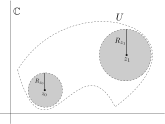
\includegraphics[width=0.5\linewidth]{Figuras/func-analitica-1}
\caption{Nesta figura mostramos como os vários discos de convergência, das expansões em série de potencias de uma função analítica $f$ definida em $U$ poderiam ter raios distintos.}
\label{fig:func-analitica-1}
\end{figure}


Duas observações são importantes neste momento. Primeiro, em geral, 
os coeficientes $a_n$ podem depender da escolha do ponto $z_0$
e talvez o mais apropriado fosse denotar estes coeficientes por $a_n(z_0)$,
para se deixar mais explícito que há esta dependência.
Segundo, se $f:U\to\mathbb{C}$ é uma função analítica, então 
como consequência do Teorema \ref{teo-diff-serie-pot-centro-z0}, 
temos que $f$ possui infinitas derivadas, 
em qualquer ponto de seu domínio e, além do mais, o 
Corolário \ref{cor-serie-taylor-para-serie-pot-centro-z0} afirma que 
\[
a_n \equiv a_n(z_0) = \frac{f^{(n)}(z_0)}{n!}, \qquad \forall n\in\mathbb{N}\cup\{0\}.
\]


Um dos principais resultados desta seção afirma 
que uma série de potências centrada em $w\in\mathbb{C}$, 
com raio de convergência $R_{w}>0$; 
define em seu disco de convergência uma função 
$f:D(w,R_{w})\to\mathbb{C}$ que é analítica. 

Para provar este resultado precisaremos 
enunciar e provar alguns fatos auxiliares sobre troca de ordem de
somas infinitas e a fórmula do Binômio de Newton para váriáveis complexas. 

É importante observar que analiticidade de uma função definida por 
uma série de potências também pode ser obtida 
como consequência da Fórmula Integral de Cauchy. 
Na verdade, no contexto de variáveis complexas, diria que esta
seria a rota mais natural para provar este fato. 
Mas isto requer ferramentas que só serão vistas mais a frente, 
quando estivermos apresentando a teoria de integração complexa. 

Uma vantagem da abordagem desenvolvida nesta seção é que ela se adapta
muito facilmente para outros contextos mais gerais 
em que também podemos definir séries de potências, mas não dispomos
de uma ferramenta como a Fórmula Integral de Cauchy.
Por exemplo, podemos aplicar as ideias desta seção 
para estudar analiticidade de séries de potências definidas
em certos espaços de Banach de dimensão infinita. 

\begin{teorema}\label{teo-fubini-discreto}
Para cada par $n,m\in \mathbb{N}\cup\{0\}$ seja $a_{n,m}$ um número complexo.
Suponha que para cada índice $n\in\mathbb{N}\cup\{0\}$ fixado, que a série 
formada pela sequência $(a_{n,m})_{m\in\mathbb{R}\cup\{0\}}$ converge
absolutamente e que a soma dos 
valores absolutos é dada por
\[
\sum_{m=0}^{\infty} |a_{n,m}| = L_n.
\]
Além do mais, assuma que a série formada por estas somas, isto é, 
$\sum_{n=0}^{\infty} L_n = A$ também é convergente. 

Então as seguintes
séries são convergentes e valem as seguintes igualdades:
\begin{itemize}
\item 
$
\displaystyle \sum_{n=0}^{\infty}\sum_{m=0}^{\infty}|a_{n,m}|
=
\sum_{m=0}^{\infty}\sum_{n=0}^{\infty}|a_{n,m}|;
$

\item 
para cada $m\in\mathbb{N}\cup\{0\}$ fixado,\qquad  $\displaystyle \sum_{n=0}^{\infty} a_{nm} \equiv C_m$;

\item 
$
\displaystyle
\sum_{n=0}^{\infty}\sum_{m=0}^{\infty}a_{n,m} 
=
\sum_{m=0}^{\infty}\sum_{n=0}^{\infty}a_{n,m}.
$
\end{itemize}

\end{teorema}

\bigskip 


O Teorema \ref{teo-fubini-discreto} pode ser visto como uma versão do Teorema
de Fubini sobre integrais iteradas. Para isto basta olharmos 
para $a_{n,m}$ como imagem de uma
função de duas variáveis 
$g:(\mathbb{N}\cup\{0\})\times(\mathbb{N}\cup\{0\})\to\mathbb{R}$.
Deste ponto de vista a conclusão do teorema poderia ser interpretada 
como a afirmação de que a soma dupla pode ser vista como
somas iteradas nas primeira e segunda variáveis, respectivamente, 
e que a ordem das somas podem ser intercambiadas. Ou de maneira
mais intuitiva. Se pensamos na lista de $a_{n,m}$'s como uma espécie 
de matrix com infinitas linhas e infinitas colunas. 
O Teorema \ref{teo-fubini-discreto} 
afirma que podemos primeiro somar cada linha desta matriz e em seguida
somar estas somas e que isto é igual a somar as colunas da matriz e 
depois somar estas somas.

\begin{figure}[H]
\centering
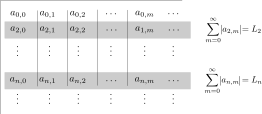
\includegraphics[width=0.75\linewidth]{Figuras/fubini-anm}
\caption{Pensando em toda a lista de $a_{n,m}$'s como uma espécie de matrix com infinitas linhas e infinitas colunas. A hipótese do Teorema \ref{teo-fubini-discreto} é que a soma dos valores absolutos das linhas desta matriz formam um nova sequência $(L_n)_{n\in\mathbb{N}\cup\{0\}}$ cuja a série associada é converge.}
\label{fig:fubini-anm}
\end{figure}


Outra maneira de pensar no Teorema \ref{teo-fubini-discreto} é vendo
que ele se trata de um resultado sobre troca de ordem de limites.
Para deixar isto mais claro vamos reescrever as séries
que aparecem na conclusão deste teorema, como limite de suas somas parciais 
(o que por definição é o que elas realmente são). 


Primeiro observe que
\begin{align}\label{eq-aux1-limite-duplo}
\sum_{n=0}^{\infty}\sum_{m=0}^{\infty}a_{n,m}
=
\lim_{p\to\infty}\sum_{n=0}^{p}\lim_{q\to\infty} \sum_{m=0}^{q}a_{n,m} 
=
\lim_{p\to\infty} \lim_{q\to\infty} \sum_{n=0}^{p} \sum_{m=0}^{q}a_{n,m}, 
\end{align}
onde na última igualdade usamos que para cada $p$ fixado que podemos
permutar a ordem da soma em $n$ com limite em $q$ por causa de uma propriedade
elementar de limite de sequências que afirma que a soma 
dos limites é o limite da soma,
quando cada um dos limites existem. O que justifica a última 
igualdade em \eqref{eq-aux1-limite-duplo}, ou seja,
\[
\sum_{n=0}^{p}\lim_{q\to\infty} \sum_{m=0}^{q}a_{n,m} 
=
\lim_{q\to\infty} \sum_{n=0}^{p}\sum_{m=0}^{q}a_{n,m}. 
\]
\bigskip 


Analogamente, temos 
\begin{align}\label{eq-aux2-limite-duplo}
\sum_{m=0}^{\infty}\sum_{n=0}^{\infty}a_{n,m}
=
\lim_{q\to\infty}\sum_{m=0}^{q}
\lim_{p\to\infty} \sum_{n=0}^{p}
a_{n,m} 
=
\lim_{q\to\infty} 
\lim_{p\to\infty} 
\sum_{n=0}^{q} 
\sum_{m=0}^{p}
a_{n,m}. 
\end{align}

Já que para cada $p,q\in\mathbb{N}$ (finitos) obviamente temos:
\begin{align}
\label{eq-aux3-limite-duplo}
S(p,q) 
\equiv 
\sum_{n=0}^{q} \sum_{m=0}^{p}a_{n,m} 
= 
\sum_{m=0}^{p}\sum_{n=0}^{q} a_{n,m}. 
\end{align}

A grande conclusão do Teorema \ref{teo-fubini-discreto} é que
as expressões do lado direito de \eqref{eq-aux1-limite-duplo}
e \eqref{eq-aux2-limite-duplo} são iguais e consequentemente 
\[
\lim_{p\to\infty} \lim_{q\to\infty} \sum_{n=0}^{p} \sum_{m=0}^{q}a_{n,m}
=
\lim_{q\to\infty}\lim_{p\to\infty} \sum_{n=0}^{p} \sum_{m=0}^{q}a_{n,m}.
\]
Em outras palavras, usando \eqref{eq-aux3-limite-duplo}, podemos simplificar
a expressão acima para
\[
\lim_{p\to\infty} \lim_{q\to\infty} S(p,q)
=
\lim_{q\to\infty}\lim_{p\to\infty} S(p,q).
\]

A igualdade acima poderia, aparentemente, soar como uma resultado muito natural. 
Porém o seguinte contra-exemplo ilustra como a conclusão do Teorema
\ref{teo-fubini-discreto} é altamente não-trivial.

\begin{exemplo}
Para cada par de números naturais $p,q\in\mathbb{N}$ defina 
\[
S(p,q) =  \frac{p}{p+q}.
\]
Então 
\[
\lim_{p\to\infty} \lim_{q\to\infty} S(p,q)
= 
\lim_{p\to\infty} \lim_{q\to\infty} \frac{p}{p+q}
= 
\lim_{p\to\infty} 0
=0
\]
e por outro lado 
\[
\lim_{q\to\infty}\lim_{p\to\infty} S(p,q)
=
\lim_{q\to\infty} \lim_{p\to\infty} \frac{p}{p+q}
=
\lim_{q\to\infty} 1
=1.
\]
Ou seja, em geral, não podemos inverter a ordem com que tomamos
limites.
\end{exemplo}


O Teorema \ref{teo-fubini-discreto} será uma das principais ferramentas utilizadas 
para mostrar que uma função $f$ dada por uma série
de potências em seu disco de convergência $D(z_0,R)$, com $R>0$,  
é uma função analítica.

A princípio, um leitor mais desatento, poderia inicialmente suspeitar de 
que não há nada a fazer, já que nossa função 
$f:D(z_0,R)\to\mathbb{C}$, por hipótese, é dada
por um série de potências, isto é,
\[
f(z) = \sum_{n=0}^{\infty}a_n(z-z_0)^n. 
\]

Mas alertamos que a questão delicada que se coloca aqui 
é que a definição de analiticidade,
exige que $f$ possa ser expressa como série de potências com raio 
de convergência positivo em torno de qualquer ponto do seu domínio. 
Isto é, dado
$z_1\in D(z_0,R)$ qualquer, diferente de $z_0$, a dificuldade técnica que 
se apresenta é: como garantir
que existem coeficientes $(b_n)_{n\in\mathbb{N}\cup\{0\}}$ 
e $R_{z_1}>0$ tais que $f$ possa ser representada como uma 
série de potências em torno deste novo ponto $z_1$, ou seja,
\[
f(z) = \sum_{n=0}^{\infty} b_n(z-z_1)^n, \qquad \forall z\in D(z_1,R_{z_1}).
\]
Em outras palavras, precisamos entender o que acontece quando mudamos
o ponto onde centramos a expansão em série de potencias de $f$. 
Isto passa por entender como se relacionam os coeficientes de cada 
uma destas expansões bem como os raios dos discos de convergência,
respectivos. 

Antes porém, precisamos de mais um resultado preparatório
que consiste em uma generalização, para números complexos, 
da famosa fórmula do Binômio de Newton

\begin{proposicao}[Binômio de Newton]
\label{prop-binom-newton}
\index{Binômio de Newton}
Para quaisquer $z,w\in\mathbb{C}$ e $n\in\mathbb{N}$ temos 
\begin{align}\label{eq-form-binom-newton}
(w+z)^n = \sum_{k=0}^n \binom{n}{k}z^{k}w^{n-k}, 
\quad \text{onde}\quad \binom{n}{k} = \frac{n!}{(n-k)!k!}.
\end{align}
\end{proposicao}

% \begin{proof}
% Observamos que é possível apresentar uma prova desta proposição 
% usando argumentos idênticos a maioria
% daqueles empregados nas provas em que $z$ e $w$ são 
% números reais. Praticamente os seguindo \textit{ipsis litteris}.  
% Isto porque a maioria destas provas, no caso real, 
% só se utiliza da estrutura de corpo de $\mathbb{R}$
% e das relações de Stifel para os coeficientes binomiais.

% \medskip 

% Por questão de completude, vamos apresentar aqui
% uma prova alternativa da validade desta proposição,
% que é enunciada para números complexos, explorando a fórmula do 
% Binômio de Newton conhecida para números reais. 

% Para isto, primeiro observamos que para todo $x\in\mathbb{R}$, temos
% da fórmula do Binômio de Newton, para números reais, que
% \[
% (1+x)^n = \sum_{k=0}^n \binom{n}{k}x^k.
% \]
% Olhando com cuidado a identidade acima, o leitor pode observar que ela
% revela que $x=-1$ é uma raíz, de 
% multiplicidade $n$, do polinômio $p:\mathbb{R}\to\mathbb{R}$,
% de grau $n$, dado por
% \[
% p(x) = \sum_{k=0}^n \binom{n}{k}x^k.
% \]

% Considere agora a função polinomial $P:\mathbb{C}\to\mathbb{C}$ 
% cujos os coeficientes são os mesmos de $p(x)$, isto é, 
% \[
% P(z) = \sum_{k=0}^n \binom{n}{k}z^k.
% \]
% Já que os coeficientes dos polinômios $p$ e $P$ são os mesmos, temos que 
% $\mathrm{grau}(P)=n$,
% e que $z=-1$ também é uma raíz de $P$ de multiplicidade $n$.
% Pois toda raíz de $p$ é obviamente uma raíz de $P$. Eventualmente, poderíamos imaginar que
% $P$ poderia ter raízes outras complexas com parte imaginária  não-nula.
% Mas isto não pode acontecer por causa do 
% algoritmo de divisão de Euclides para polinômios,
% que garante que $(z+1)^n$ é um fator de $P(z)$. 
% Mas como $\mathrm{grau}(P)=n$ então sua fatoração é exatamente 
% esta $(z+1)^n$. Assim temos
% \[
% \sum_{k=0}^n \binom{n}{k}z^k  = P(z) = (z+1)^n, \qquad \forall z\in\mathbb{C} 
% \]

% Agora podemos usar a identidade acima para 
% verificar a validade de fórmula do Binômio de Newton 
% para quaisquer $z\in\mathbb{C}$ e 
% $w\in\mathbb{C}\setminus\{0,-z\}$. De fato, 
% \begin{align*}
% (w+z)^n 
% = 
% w^n\Big(1+\frac{z}{w}\Big)^n 
% = 
% w^n 
% P\Big(\frac{z}{w}\Big) = 
% w^n
% \sum_{k=0}^n \binom{n}{k}\frac{z^k}{w^k}
% =
% \sum_{k=0}^n \binom{n}{k}z^k\,w^{n-k}.
% \end{align*}

% Para finalizar a prova, basta observar que \eqref{eq-form-binom-newton}
% é obviamente verdadeira nos casos em que $w=0$ ou $w=-z$.
% \end{proof}

\bigskip

Para cada $n\in\mathbb{N}\cup\{0\}$ fixado, considere a função
$\mathds{1}_{[n]}:\mathbb{N}\cup\{0\}\to\{0,1\}$ dada por 
\begin{align}\label{eq-def-1mn}
\mathds{1}_{[n]}(m)
\equiv
\begin{cases}
1,\quad\text{se}\ 0\leqslant m\leqslant n;
\\[0.2cm]
0,\quad\text{caso contrário}.
\end{cases}
\end{align}

Note que a função $\mathds{1}_{[n]}(m)$ assume o valor $1$ se seu argumento  $m\in\{0,1,2,\ldots,n\}$ e assume o valor
zero caso $m>n$. 
Vamos usar estas funções na prova do próximo teorema para expressar somas finitas como 
séries infinitas. Em particular, vamos usar a seguinte identidade
\begin{align}\label{eq-aux1-indicadora-[m]}
\sum_{m=0}^n \mathds{1}_{[n]}(m)\, c_n = \sum_{m=0}^{\infty} \mathds{1}_{[n]}(m)\, c_n,
\end{align}
válida para qualquer $n\in\mathbb{N}\cup\{0\}$ fixado e $(c_n)_{n\in\mathbb{N}\cup\{0\}}$ qualquer sequência de números complexos
(observe que nesta identidade não é preciso nem mesmo 
exigir que a serie dos $c_n$'s seja convergente). 
Na verdade, 
nesta identidade a série que aparece no lado direito 
têm todos os termos de índice maior que $n$
nulos, pela definição de $\mathds{1}_{[n]}(m)$. 

Outra identidade importante na prova do próximo teorema 
e que segue diretamente da definição de $\mathds{1}_{[n]}(m)$ é a seguinte: 
para cada $n\in\mathbb{N}\cup\{0\}$ fixado temos
\begin{align}\label{eq-aux2-indicadora-[m]}
\sum_{m=0}^{\infty} 
\mathds{1}_{[n]}(m)\, c_n 
= 
\sum_{m=n}^{\infty} \mathds{1}_{[n]}(m)\, c_n.
\end{align}


Finalmente estamos prontos para mostrar o resultado mais importante
desta seção.

\bigskip 

\begin{teorema}\label{teo-series-pot-analiticas}
Se $f:D(z_0,R)\to\mathbb{C}$ é uma função definida 
por uma série de potencias, com coeficientes complexos 
$(a_n)_{n\in\mathbb{N}\cup\{0\}}$, centrada
em $z_0\in\mathbb{C}$, com raio de convergência $R>0$. Ou seja,
\[
f(z) = \sum_{n=0}^{\infty} a_n(z-z_0)^n, \qquad \forall z\in D(z_0,R).
\]
Então $f:D(z_0,R)\to\mathbb{C}$ é uma função analítica, isto é, 
para qualquer $z_1\in D(z_0,R)$ fixado, existem 
coeficientes complexos $(b_n)_{n\in\mathbb{N}\cup\{0\}}$ 
e um número positivo $R_{z_1}=R-|z_1-z_0|$
tais que 
\[
f(z) = \sum_{n=0}^{\infty} b_n(z-z_1)^n, \qquad \forall z\in D(z_1,R_{z_1}).
\] 
\end{teorema}

\begin{figure}[H]
\centering
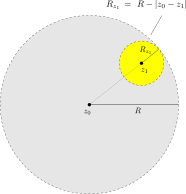
\includegraphics[width=0.55\linewidth]{Figuras/Rz1-func-analitica}
\caption{O raio de convergência da série de potencias centrada em $z_1$ é pelo menos $R_{z_1}=R-|z_0-z_1|$.}
\label{fig:rz1-func-analitica}
\end{figure}


\begin{proof}
Vamos decompor a prova em duas partes. Na primeira parte vamos assumir
que a série de potências está centrada na origem, isto é, $z_0=0$. 
Em seguida, vamos mostrar que o caso geral, $z_0\in\mathbb{C}$ qualquer, 
pode ser reduzido ao caso tratado na primeira parte, 
fazendo uma simples mudança de variáveis.

\bigskip 
\noindent\textbf {Parte 1.}
Como mencionado acima, vamos assumir nesta primeira parte da prova que 
\[
f(z) = \sum_{n=0}^{\infty} a_n z^n, \qquad \forall z\in D(0,R). 
\]
Fixado um ponto arbitrário $z_1\in D(0,R)$ defina $R_{z_1}\equiv R-|z_1|$.


\medskip 

Para cada $m,n\in \mathbb{N}\cup\{0\}$ defina
\[
a_{n,m} = \mathds{1}_{[n]}(m) \cdot a_n \cdot \binom{n}{m} z_1^{n-m}(z-z_1)^{n}, 
\]
onde $\mathds{1}_{[n]}(m)$ é definido como em \eqref{eq-def-1mn}.


Vamos mostrar que os $a_{n,m}$'s satisfazem as hipóteses 
do Teorema \ref{teo-fubini-discreto}, se tomamos $z\in D(z_1,R_{1})$,
onde $R_1=R-|z_1|$. 
Para provar isto, primeiro observamos que 
\[
|a_{n,m}| 
= 
\mathds{1}_{[n]}(m) \cdot |a_n| \cdot \binom{n}{m} |z_1|^{n-m}(|z-z_1|)^{n}. 
\]
E portanto segue da igualdade \eqref{eq-aux1-indicadora-[m]} e da fórmula do Binômio
de Newton (Proposicão \ref{prop-binom-newton}) que para cada  $n\in \mathbb{N}\cup\{0\}$
fixado temos
\begin{align*}
L_n 
\equiv 
\sum_{m=0}^{\infty}|a_{n,m}| 
&=
\sum_{m=0}^{\infty}\mathds{1}_{[n]}(m) \cdot |a_n| \cdot \binom{n}{m} |z_1|^{n-m}(|z-z_1|)^{n} 
\\
&=
\sum_{m=0}^{n} |a_n| \cdot \binom{n}{m} |z_1|^{n-m}(|z-z_1|)^{n} 
\\
&=
|a_n| \sum_{m=0}^{n} \binom{n}{m} |z_1|^{n-m}(|z-z_1|)^{n} 
\\
&=
|a_n| (|z-z_1|+|z_1|)^{n}. 
\end{align*}
Agora note que se tomamos $z\in D(z_1,R_{1})$, então temos $|z-z_1|<R-|z_1|$ e portanto 
$|z-z_1|+|z_1|<R$. Logo temos das propriedades elementares de séries de potencia 
que a série abaixo é convergente
\begin{align*}
\sum_{n=0}^{\infty} L_n = \sum_{n=0}^{\infty} |a_n| (|z-z_1|+|z_1|)^{n}.
\end{align*}
O que mostra que as hipóteses do Teorema \ref{teo-fubini-discreto} são
válidas desde que $z\in D(z_1,R_{1})$. 

\bigskip 
Portanto sob a condição $z\in D(z_1,R_{1})$ poderemos aplicar o Teorema \ref{teo-fubini-discreto} e com isto garantir
a convergência de todas as séries que aparecem abaixo bem como a mudança de 
na ordem das somas feita na nona igualdade abaixo. 
Para facilitar a compreensão pelo leitor, 
observamos também que para a sexta igualdade
que aparece abaixo basta usar \eqref{eq-aux1-indicadora-[m]} e para penúltima
igualdade é só aplicar \eqref{eq-aux2-indicadora-[m]}
\begin{align*}
f(z)
&=
\sum_{n=0}^{\infty} a_nz^n
=
\sum_{n=0}^{\infty} a_n(z-z_1+z_1)^n
\\
&=
\sum_{n=0}^{\infty} a_n \left[ \sum_{m=0}^n \binom{n}{m}z_1^{n-m}(z-z_1)^m  \right]
=
\sum_{n=0}^{\infty}  \left[ \sum_{m=0}^n a_n\binom{n}{m}z_1^{n-m}(z-z_1)^m  \right]
\\
&=
\sum_{n=0}^{\infty}  \left[ \sum_{m=0}^n 
\mathds{1}_{[m]}(n)\cdot a_n\cdot \binom{n}{m}z_1^{n-m}(z-z_1)^m  \right]
\\
&=
\sum_{n=0}^{\infty}  \left[ \sum_{m=0}^{\infty} 
\mathds{1}_{[m]}(n)\cdot a_n\cdot \binom{n}{m}z_1^{n-m}(z-z_1)^m  \right]
\\
&=
\sum_{n=0}^{\infty}  
\sum_{m=0}^{\infty} 
\mathds{1}_{[m]}(n)\cdot a_n\cdot \binom{n}{m}z_1^{n-m}(z-z_1)^m  
\\
&=
\sum_{n=0}^{\infty}  
\sum_{m=0}^{\infty} 
a_{n,m}
=
\sum_{m=0}^{\infty} 
\sum_{n=0}^{\infty}  
a_{n,m}
\\
&=
\sum_{m=0}^{\infty} \sum_{n=0}^{\infty} 
\mathds{1}_{[n]}(m)\cdot a_n\cdot \binom{n}{m}z_1^{n-m}
(z-z_1)^m
\\
&=
\sum_{m=0}^{\infty}  \left[ \sum_{n=0}^{\infty} 
\mathds{1}_{[n]}(m)\cdot a_n\cdot \binom{n}{m}z_1^{n-m}  \right]
(z-z_1)^m
\\
&=
\sum_{m=0}^{\infty}  
\left[ 
\sum_{n=m}^{\infty}  a_n\cdot \binom{n}{m}z_1^{n-m}  \right]
(z-z_1)^m
\\
&=
\sum_{m=0}^{\infty} b_m(z-z_1)^m,
\end{align*}
onde na última igualdade usamos a notação
\begin{align}\label{eq-aux1-teo-series-pot-analiticas}
b_m \equiv \sum_{n=m}^{\infty}  a_n\cdot \binom{n}{m}z_1^{n-m}.
\end{align}

\bigskip 

\noindent\textbf {Parte 2.}
Para provar o teorema quando $z_0$ não é necessariamente zero.
Basta consideramos a mudança de variável $w=z-z_0$.

Fazendo isto temos 
\[
\sum_{n=0}^{\infty}a_n(z-z_0)^n 
=
\sum_{n=0}^{\infty}a_n w^n 
\]
com a série à direta, sendo absolutamente convergente para todo $|w|<R$.

Dado $z_1\in D(z_0,R)$ seja $w_1=z_1-z_0$. É claro que pela escolha
de $z_1$ que temos $|w_1|=|z_0-z_1|<R$.

Note que podemos aplicar o resultado obtido na 
primeira parte da prova, para concluir que 
para todo $w\in D(w_1,R-|w_1|)$ temos:
\[
\sum_{n=0}^{\infty}a_n w^n
=
\sum_{n=0}^{\infty}b_n (w-w_1)^n, \qquad \forall |w-w_1|<R-|w_1|.
\]
Lembrando que $w=z-z_0$ e $w_1=z_1-z_0$, concluímos finalmente da
igualdade acima que 
\[
f(z)
=
\sum_{n=0}^{\infty}a_n (z-z_0)^n
=
\sum_{n=0}^{\infty}b_n \big(\,(z-z_0) -(z_1-z_0)\, \big)^n
=
\sum_{n=0}^{\infty}b_n (z-z_1)^n,
\]
para todo $z\in\mathbb{C}$ satisfazendo $|z-z_1|<R-|w_1|=R-|z_0-z_1|$.
\end{proof}

\bigskip

Há varias observações importante que devem ser feitas sobre o teorema que acabamos
de demonstrar. 


\bigskip 


Primeiro, começamos com nossa função $f:D(z_0,R)\to\mathbb{C}$
dada pela série de potências 
\[
f(z)=\sum_{n=0}^{\infty}a_n(z-z_0)^n.
\]
O mais natural aqui, é que $R$ tenha sido tomado como sendo o raio de convergência 
desta série, que é dado por
\[
R = \frac{1}{\displaystyle\limsup_{n\to\infty} \sqrt[n]{|a_n|}}
\]

O Teorema \ref{teo-series-pot-analiticas} mostra que 
quando mudamos o centro da série de potencias então 
passamos de uma representação de
\[
f(z) = \sum_{n=0}^{\infty}a_n(z-z_0)^n,
\quad \text{válida para todo}\  z\in D(z_0,R),
\] 
para uma nova representação
\begin{align}\label{eq-aux-exe-muda-centro-serie}
f(z) = \sum_{n=0}^{\infty}b_n(z-z_1)^n,
\qquad \text{válida para todo}\ z\in D(z_1,R_1).
\end{align}


Como vimos a série acima converge absolutamente em todo ponto do 
disco $D(z_1,R_1)$, onde $R_1=R-|z_0-z_1|$. Portanto, segue do teorema de existência 
do raio de convergência (\,Teorema \ref{teo-exist-raio-conv} item \textit{(iii)}\,) que
\[
R_{z_1} 
\leqslant 
\frac{1}{\displaystyle\limsup_{n\to\infty} \sqrt[n]{|b_n|}}
\equiv 
\widetilde{R}_{z_1},
\] 
veja Figura \ref{fig:raio-func-analitica-muda-centro}. 

A priori não há nada que proíba a desigualdade acima de ser estrita. 
A ocorrência deste fato é inclusive ligada 
a manifestação de um fenômeno muito importante.
Neste caso, a função $f$ irá admitir uma extensão analítica para além do disco $D(0,R)$!
Para esclarecer este comentário, precisamos 
da definição de extensão analítica de uma função. 

\begin{definicao}[Extensão Analítica]
\label{def-ext-analitica}
\index{Extensão!analítica}
Sejam $U\subset\mathbb{C}$ um conjunto aberto não vazio e
$f:U\to\mathbb{C}$ uma função analítica. Dizemos que $f$ admite
uma extensão analítica à um aberto $V\subset \mathbb{C}$,
contendo $U$ estritamente ($U\subsetneq V$), se existe e uma função analítica $F:V\to\mathbb{C}$ 
tal que $F|_{U}= f$. Isto é, a restrição de $F$ ao conjunto $U$ 
é exatamente a função $f$. 
\end{definicao}


Voltando a discussão acima, se ocorrer $R_{z_1} < \widetilde{R}_{z_1}$
temos que a série de potências em \eqref{eq-aux-exe-muda-centro-serie} 
converge em um ponto $z$ que está
fora do disco $D(z_0,R)$, onde, a rigor, não faria muito sentido falar
de $f(z)$, já que este ponto está fora do domínio da função $f$.
Mas esta observação, nos motiva naturalmente, a definir uma extensão 
analítica de $f$ da seguinte forma. O domínio na nossa extensão será o 
o conjunto $V \equiv D(z_0,R)\cup D(z_1,\widetilde{R}_{z_1})$ e a função
$F:V\to\mathbb{C}$ é dada por 
\[
F(z)
=
\begin{cases}
\displaystyle\sum_{n=0}^{\infty}a_n(z-z_0)^n,&\ \text{se}\ z\in D(z_0,R);
\\[0.9cm]
\displaystyle\sum_{n=0}^{\infty}b_n(z-z_1)^n,&\ \text{se}\ z\in D(z_1,\widetilde{R}_{z_1}).  
\end{cases}
\]

\bigskip 

\begin{figure}[H]
\centering
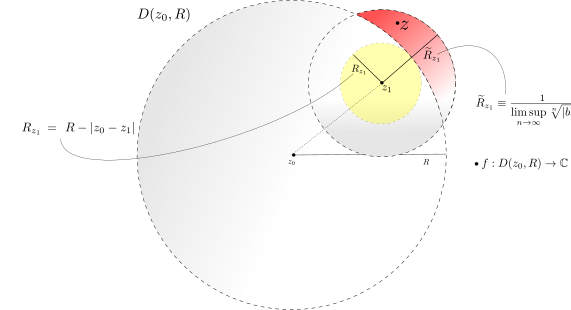
\includegraphics[width=0.95\linewidth]{Figuras/Raio-func-analitica-muda-centro}
\caption{Note que apesar da série de potencias \eqref{eq-aux-exe-muda-centro-serie}, 
centrada em $z_1$ fazer sentido, para qualquer ponto $z$ na região hachurada em vermelho (exterior ao disco $D(z_0,R))$, a rigor, não faz sentido falar de $f(z)$.}
\label{fig:raio-func-analitica-muda-centro}
\end{figure}


Observe que não há ambiguidade na definição acima já que para 
todo $z$ satisfazendo $z\in D(z_0,R)$ e $z\in D(z_1,\widetilde{R}_{z_1})$, isto é, 
\[
z\in D(z_0,R)\cap D(z_1,\widetilde{R}_{z_1})
\] 
temos do Teorema \ref{teo-series-pot-analiticas} que
\[
\sum_{n=0}^{\infty}a_n(z-z_0)^n
=
\sum_{n=0}^{\infty}b_n(z-z_1)^n
\]
e portanto que o valor $F(z)$ está bem definido. 

\medskip 
Claramente temos $F|_{D(z_0,R)} = f$. De fato, se $z\in D(z_0,R)$ segue diretamente das
definições de $F$ e $f$, respectivamente, que 
\[
F(z) = \sum_{n=0}^{\infty}a_n(z-z_0)^n = f(z).
\]

Para verificar que $F$ é analítica precisamos aplicar o 
Teorema \ref{teo-series-pot-analiticas}. 
De fato, para qualquer $z_2\in V= D(z_0,R)\cup D(z_1,\widetilde{R}_{z_1})$ dado,
temos que ou $z_2\in D(z_0,R)$ ou $z_2\in D(z_1,\widetilde{R}_{z_1})$.

\medskip
\noindent
\textbf{Caso 1.} Se $z_2\in D(z_0,R)$ 
então o Teorema \ref{teo-series-pot-analiticas} garante
que existem coeficientes $(c_n)_{n\in\mathbb{N}\cup\{0\}}$ tais que 
\[
F(z) 
= 
\sum_{n=0}^{\infty}a_n(z-z_0)^n 
= 
\sum_{n=0}^{\infty}c_n(z-z_2)^n, \qquad \forall z\in D(z_2,R-|z_0-z_2|).
\]
o que significa que $F$ admite uma representação em séries de potências
centrada em $z_2$ com raio de convergência positivo 
$\widetilde{R}_{z_2} \geqslant R_{z_2}\equiv R-|z_0-z_2|$.

\medskip
\noindent
\textbf{Caso 2.}
Analogamente, se $z_2\in D(z_1,\widetilde{R}_{z_1})$ então temos novamente 
do Teorema \ref{teo-series-pot-analiticas} que existem coeficientes 
$(d_n)_{n\in\mathbb{N}\cup\{0\}}$ tais que 
\[
F(z) 
= 
\sum_{n=0}^{\infty}b_n(z-z_1)^n  
= 
\sum_{n=0}^{\infty}d_n(z-z_2)^n, \qquad \forall z\in D(z_2,\widetilde{R}_{z_1}-|z_1-z_2|).
\]
o que assegura, que também neste caso, $F$ admite uma representação em série
de potências, centrada em $z_2$, com raio de convergência 
$\widetilde{R}_{z_2}\geqslant R_{z_2}\equiv \widetilde{R}_{z_1}-|z_1-z_2|>0$.

\medskip 

Mais a frente, vamos discutir a importante questão 
sobre existência e unicidade de extensões analíticas de uma função.

\medskip


A segunda observação importante sobre o Teorema \ref{teo-series-pot-analiticas}
é que se uma série de potências, centrada em $z_0$, 
tem raio de convergência infinito, ou seja,
se $f:\mathbb{C}\to\mathbb{C}$ é dada por 
\[
f(z) = \sum_{n=0}^{\infty} a_n(z-z_0)^n,\qquad \forall z\in\mathbb{C}
\]
então qualquer que seja $z_1$ em $\mathbb{C}$, existem coeficientes 
$(b_n)_{n\in\mathbb{N}\cup\{0\}}$ tais que 
\[
f(z) = \sum_{n=0}^{\infty} b_n(z-z_1)^n, \qquad \forall z\in\mathbb{C}.
\]
Em outras palavras, se mudamos o centro de uma série de potências 
com raio de convergência infinto, que representa $f$, 
então obtemos uma nova série de potências que representa $f$
e que também tem raio de convergência infinito.


\bigskip

A terceira observação é o seguinte corolário.

\begin{corolario}\label{cor-coeficientes-func-analiticas}
Seja $U\subset\mathbb{C}$ um conjunto aberto e $f:U\to\mathbb{C}$
uma função analítica. Então para cada $z_0\in U$, existe 
$R_{z_0}\in (0,+\infty]$ (positivo estrito) tal que 
\[
f(z) = \sum_{n=0}^{\infty} \frac{f^{(n)}(z_0)}{n!}(z-z_0)^n,
\qquad \forall z\in D(z_0,R_{z_0}).
\]
\end{corolario}

\begin{proof}
Já que $f$ é analítica, temos por definição que para qualquer $z_0\in U$ 
fixado, existem coeficientes $(a_n)_{n\in\mathbb{N}\cup\{0\}}$ e um 
raio de convergência positivo $R_{z_0}$ tais que 
\[
f(z) = \sum_{n=0}^{\infty} a_n(z-z_0)^n,
\qquad \forall z\in D(z_0,R_{z_0}).
\]
Pelo Teorema \ref{teo-diff-serie-pot-centro-z0} e Corolário \ref{cor-serie-taylor-para-serie-pot-centro-z0} a função $f$ 
tem derivadas complexas de todas as ordens e além do mais 
a $n$-ésima derivada de $f$ calculada em $z_0$ satisfaz
\[
a_n = \frac{f^{(n)}(z_0)}{n!}.
\]
\end{proof}



\begin{exemplo}\label{exe-pol-serie-pot}
Se $p:\mathbb{C}\to\mathbb{C}$ é uma função polinomial da forma 
\[
p(z) = a_0+a_1z+a_2z^2+\ldots +a_nz^{n}
\]
então $p$ é uma função analítica.
\end{exemplo}

Escolhemos apresentar e discutir, em detalhes, este exemplo porque
ele ilustra de maneira simples e explícita vários dos conceitos 
e resultados apresentados acima. A ideia apresentada a seguir será fundamental
para estabelecermos vários resultados importantes sobre funções
analíticas. 

\medskip 

Primeiro observe que é possível reconhecer $p$ como 
uma série de potências. 
De fato, considere a sequência $(b_k)_{k\in\mathbb{N}}$
dada por:
\[
b_0=a_0,\quad b_1=a_1,\ \ldots,\quad b_n=a_n,\quad  b_{n+1}=0,\quad b_{n+2}=0,\ \ldots
\]
Então temos para todo $z\in \mathbb{C}$
\[
p(z) = a_0+a_1z+\ldots+a_nz^n = \sum_{k=0}^{\infty} b_kz^k.
\]
Desta forma vemos que $p$ é uma série de potências centrada em zero, com
raio de convergência infinito. Na verdade, esta observação sobre o raio é simplesmente 
uma consequência do lado direito da expressão acima ser uma soma
finita. Este fato óbvio também poderia ser obtido a partir da fórmula 
do raio de convergência, já que, 
\begin{align*}
\limsup_{k\to\infty} \sqrt[k]{|b_k|}
&\equiv 
\lim_{k\to\infty} \left[ \sup \Big\{ \sqrt[k]{|b_k|}, \sqrt[k+1]{|b_{k+1}|}, \sqrt[k+2]{|b_{k+2}|},\ldots  \Big\} \right].
\end{align*}
Pela definição de $b_k$, temos para todo $k>n =\textrm{grau}(p)$ que 
$\sqrt[k]{|b_k|}=0$. Logo a expressão acima, 
é igual a $\lim_{k\to\infty} \sup\{0\} = 0$. Mostrando que
$R^{-1}=0$ e assim $R=+\infty$.  

Aplicando o Teorema \ref{teo-series-pot-analiticas} podemos
concluir que $p$ é uma função analítica. 
Pelas observações feitas acima, podemos mudar o centro da expansão de $p$
para qualquer outro ponto $z_0\in\mathbb{C}$, obtendo novamente outra 
representação em séries de potência para $p$, centrada em $z_0$, com raio 
de convergência também infinito, isto é, existem coeficientes $(c_k)_{k\in\mathbb{N}\cup\{0\}}$ tais que  
\[
p(z) = \sum_{k=0}^{\infty} c_k(z-z_0)^k, \qquad \forall z\in\mathbb{C}.
\]
Do Corolário \ref{cor-coeficientes-func-analiticas} temos que
$c_k= p^{(k)}(z_0)/k!$, para todo $k\geqslant 0$ e
\[
p(z) = \sum_{k=0}^{\infty} \frac{p^{(k)}(z_0)}{k!}(z-z_0)^k, \qquad \forall z\in\mathbb{C}.
\] 
Como as derivadas de $p$ de ordem maiores que $n=\mathrm{grau}(p)$ são nulas, 
temos da igualdade acima que 
\begin{align}\label{eq-polinomio-como-serie-centro-z0}
p(z) = \sum_{k=0}^{n} \frac{p^{(k)}(z_0)}{k!}(z-z_0)^k, \qquad \forall z\in\mathbb{C}.
\end{align}

Para explora só um pouco mais este exemplo, lembramos que identidade 
\eqref{eq-aux1-teo-series-pot-analiticas} fornece uma relação explicita
entre os coeficiente da expansão em série de potencias de uma função 
analítica, quando mudamos o centro da expansão.
Neste caso particular \eqref{eq-aux1-teo-series-pot-analiticas} afirma que
\[
\frac{p^{(k)}(z_0)}{k!}
=
c_k 
= 
\sum_{j=k}^{\infty}  b_j\cdot \binom{j}{k}z_1^{j-k}
=
\sum_{j=k}^{n}  a_j\cdot \binom{j}{k}z_0^{j-k}.
\]

\begin{exemplo}\label{exe-1/z-analitica}
A função $f:\mathbb{C}^{*}\to\mathbb{C}$ dada por 
\[
f(z) = \frac{1}{z}, \qquad \forall z\in\mathbb{C}^{*}
\]
é analítica. 
\end{exemplo}

Para mostrar que $f$ é analítica, 
dado qualquer ponto $z_0\in\mathbb{C}^{*}$ temos que mostrar que
existem coeficientes $(a_n)_{n\in\mathbb{N}\cup\{0\}}$ e 
$R_{z_0}>0$ tais que 
\begin{align}\label{eq-aux3-analiticidade-1/z}
f(z) = \sum_{n=0}^{\infty} a_n(z-z_0)^n, \qquad \forall z\in D(z_0,R_{z_0}).
\end{align}

A ideia vai ser usar séries geométricas, mais precisamente a 
identidade
\begin{align}\label{eq-aux1-analiticidade-1/z}
\frac{1}{1-w} = \sum_{n=0}^{\infty} w^n, \qquad \text{válida para} \ |w|<1.
\end{align}

Dado $z_0\in\mathbb{C}^{*}$, 
observe que podemos escrever, realizando apenas manipulações algébricas simples,
a seguinte igualdade:
\begin{align}\label{eq-aux2-analiticidade-1/z}
\frac{1}{z}
=
\frac{1}{z-z_0+z_0} 
&= 
\frac{1}{\displaystyle z_0\Big( \frac{z-z_0}{z_0}  + 1\Big) } 
\nonumber\\[0.3cm]
&=
\frac{1}{z_0} \frac{1}{\displaystyle\Big( 1+\frac{z-z_0}{z_0}\Big) } 
=
\frac{1}{z_0} \frac{1}{\displaystyle\Big( 1-(-1)\frac{z-z_0}{z_0}\Big) } 
\nonumber\\
&=
\frac{1}{z_0} \frac{1}{\displaystyle\Big( 1-\frac{z-z_0}{-z_0}\Big) } 
\end{align}

Se consideramos apenas os números complexos $z$'s satisfazendo 
\[
\left| \frac{z-z_0}{-z_0} \right|<1, \qquad \text{ou seja},\qquad \ |z-z_0|<|z_0| 
\quad \Longleftrightarrow \quad z\in D(z_0,|z_0|)
\]
Podemos usar identidade \eqref{eq-aux1-analiticidade-1/z} 
na segunda fração que aparece em 
\eqref{eq-aux2-analiticidade-1/z} para concluir que 

\begin{align*}
f(z)
=
\frac{1}{z}
&=
\frac{1}{z_0} \frac{1}{\displaystyle\Big( 1-\frac{z-z_0}{-z_0}\Big) } 
\\[0.3cm]
&=
\frac{1}{z_0}\sum_{n=0}^{\infty} \left( \frac{z-z_0}{-z_0} \right)^n
\\[0.3cm]
&=
\frac{1}{z_0}\sum_{n=0}^{\infty}\frac{1}{(-1)^n \, (z_0)^n} (z-z_0)^n
\\[0.3cm]
&=
\sum_{n=0}^{\infty}\frac{(-1)^n}{(z_0)^{n+1}} (z-z_0)^n,
\qquad \forall z\in D(z_0,|z_0|).
\end{align*}

A identidade acima prova a existência de uma representação 
em série de potências para $f$, em torno de qualquer $z_0\in\mathbb{C}^{*}$, 
com raio de convergência $R_{z_0}=|z_0|>0$
e os coeficientes $a_n$'s dados por 
\[
a_n = \frac{(-1)^n}{(z_0)^{n+1}} ,\qquad \forall n\in\mathbb{N}\cup\{0\},
\]
como exigido em \eqref{eq-aux3-analiticidade-1/z}.


\bigskip

Este exemplo leva a uma observação importantíssima! 
Será que poderíamos ter concluído (apenas com os resultados que provamos até aqui) 
que $f$ é analítica 
simplesmente calculando 
\[
\frac{f^{(n)}(z_0)}{n!} = \frac{(-1)^n}{(z_0)^{n+1}}
\]
e, em seguida, mostrando que este coeficientes nos fornece uma série de
potências convergente com raio de convergência
\[
R 
= 
\frac{1}{\displaystyle\limsup_{n\to\infty} \sqrt[n]{|a_n|}}
=
\frac{1}{\displaystyle\limsup_{n\to\infty} \sqrt[n]{\left|\frac{(-1)^n}{(z_0)^{n+1}}\right|}}
=
\frac{1}{\displaystyle\frac{1}{|z_0|}}
=
|z_0|.
\]

A resposta, a rigor, é não! Até saberíamos que a série de potências
abaixo (que é a série de Taylor de $f$)
\[
\sum_{n=0}^{\infty} \frac{f^{(n)}(z_0)}{n!} (z-z_0)^n
=
\sum_{n=0}^{\infty}\frac{(-1)^n}{(z_0)^{n+1}} (z-z_0)^n,
\quad \text{converge para todo} \ z\in D(z_0,|z_0|).
\]
Mas sem qualquer informação adicional, não teríamos 
como concluir que a série acima, para cada $z$ no disco de convergência,
converge exatamente para $f(z)$. 

\subsection{Princípio da Identidade}

Nesta seção vamos estudar algumas das propriedades fundamentais 
das séries de potências e suas generalizações para funções analíticas
tomando valores em $\mathbb{C}$. 
Um dos principais objetivos é mostrar que se uma função analítica
$f:U\to\mathbb{C}$, definida em um \textbf{domínio} $U$, admite 
uma extensão analítica (no sentido da Definição \ref{def-ext-analitica}) 
à um domínio $V$ contendo $U$, então esta extensão é única.   
Este tipo de resultado mostra claramente a rigidez que a condição 
de analiticidade impõem a uma função. A figura abaixo
ilustra a peculiaridade do resultado mencionado acima, 
já que podemos construir, por exemplo, funções reais deriváveis definidas em 
um intervalo finito $(a,b)$ que 
admitem infinitas extensões deriváveis.



\bigskip 


Para começar vamos considerar as séries de potências mais simples
de todas que àquelas dadas por polinômios.
Seja $p:\mathbb{C}\to\mathbb{C}$ dada por $p(z)=a_0+a_1z+a_2z^2+\ldots+a_nz^n$.
Um polinômio não-nulo de grau $n$. Suponha que $z_0$ é seja uma raiz de $P$ e
considere sua expansão em série de potências em torno de $z=z_0$, obtida no 
Exemplo \ref{exe-pol-serie-pot},
\[
p(z) = \sum_{k=0}^{n} \frac{p^{(k)}(z_0)}{k!}(z-z_0)^k, \qquad \forall z\in\mathbb{C}.
\] 
Já que $p(z_0)=0$, o primeiro termo do somatório acima é nulo e  
portanto podemos reescrever $p$ como segue
\[
p(z)=(z-z_0)\sum_{k=1}^{n} \frac{p^{(k)}(z_0)}{k!}(z-z_0)^{k-1}, \qquad \forall z\in\mathbb{C}.
\]
Procedendo de maneira análoga podemos repetir este processo de fatoração $m$ vezes, 
onde $m$ é determinado pelas seguintes condições:
$p^{(m)}(z_0)\neq 0$, e $p^{(j)}(z_0)=0$ para todo $0\leqslant j\leqslant m-1$. 
Desta forma ficamos com
\[
p(z)=
(z-z_0)^m
\sum_{k=m}^{n} \frac{p^{(k)}(z_0)}{k!}(z-z_0)^{k-m}, \qquad \forall z\in\mathbb{C}.
\]
O valor de $m$ nada mais é do que a multiplicidade de $z_0$ como raíz de $p$.
A razão de apresentá-lo desta maneira é que o método empregado aqui poderá 
ser aplicado também para séries de potências! 

Próximo fato importante que devemos destacar sobre a fatoração obtida acima é que 
o polinômio que aparece como fator de $p(z)$, multiplicando $(z-z_0)^m$, isto é,
\[
q(z) \equiv \sum_{k=m}^{n}\frac{p^{(k)}(z_0)}{k!}(z-z_0)^{k-m} 
\]
é tal que $q(z)$ não se anula em $z=z_0$, pela definição de $m$. 
Já que função $z\longmapsto q(z)$ é contínua dado 
\[ 
\varepsilon = \frac{1}{2}\frac{|p^{(m)}(z_0)|}{m!} 
\]
existe um $\delta>0$ tal que se 
\[
0<|z-z_0|<\delta, 
\quad\text{então}\ \ 
\left| q(z) - \frac{p^{(m)}(z_0)}{m!}\right|
<
\frac{1}{2}\ \frac{|p^{(m)}(z_0)|}{m!}.
\]
Desta forma temos da segunda desigualdade triangular que
\begin{align*}
\left|\frac{p^{(m)}(z_0)}{m!}\right| - |q(z)| 
\leqslant 
\left| q(z) - \frac{p^{(m)}(z_0)}{m!}\right|
<
\frac{1}{2}\ \frac{|p^{(m)}(z_0)|}{m!}
\end{align*}
e portanto 
\[
\frac{1}{2}\ \frac{|p^{(m)}(z_0)|}{m!} <|q(z)|, 
\quad \text{para todo}\ z\ \text{satisfazendo}\ 0<|z-z_0|<\delta.
\]
Mostrando que os zeros de uma função polinomial não-nula 
são isolados. É claro que poderíamos ter chegado a esta mesma conclusão 
por outras vias mais simples. A razão de termos escolhido este argumento é que
ele se generaliza para séries de potências, fornecendo o seguinte
resultado que é de grande importância para a teoria de funções analíticas.


\begin{lema}\label{lema-centro-serie-zero-isolado}
Seja $(a_n)_{n\in\mathbb{N}\cup\{0\}}$ uma sequência de números complexos
não identicamente nula. Suponha que a série de potências 
centrada em $w\in\mathbb{C}$ e gerada por esta sequência, 
tenha raio de convergência $R>0$. 
Seja $f:D(w,R)\to\mathbb{C}$ a função dada por
\[
f(z) = \sum_{n=0}^{\infty}a_n(z-w)^n, \qquad \forall z\in D(w,R)
\]
e denote por $\mathcal{Z}(f)\equiv \{w\in\mathbb{C}: f(w)=0\}$ 
conjunto dos zeros de $f$.  Se o centro da série de potências 
$w\in \mathcal{Z}(f)$ então existe $\delta>0$ tal que 
para todo $z$ satisfazendo $0<|z-w|<\delta$ temos $z\notin \mathcal{Z}(f)$.
Em outras palavras, $w$ é um zero isolado de $f$.
\end{lema}

\begin{figure}[H]
\centering
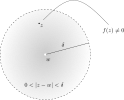
\includegraphics[width=0.45\linewidth]{Figuras/zeros-isolados1}
\caption{O único zero de $f$ dentro do conjunto $\{z\in\mathbb{C}: 0<|z-w|<\delta\}$}
\label{fig:zeros-isolados1}
\end{figure}



\begin{proof}
A prova deste lema é baseada no argumento apresentado no inicio desta seção. 

Suponha que $f(w)=0$. Então temos que $a_0=0$. 
Já que $(a_n)_{n\in\mathbb{N}\cup\{0\}}$ uma sequência de números complexos
não identicamente nula, existe $m\in\mathbb{N}$ (finito),
o primeiro índice, tal que $a_{n}=0$ para todo $0\leqslant n\leqslant m-1$
e $a_{m}\neq 0$. Portanto podemos reescrever $f$ como segue
\begin{align}\label{eq-aux1-principio-ident}
f(z) = (z-w)^{m}\sum_{n=m}^{\infty}a_{n}(z-w)^{m-n}
\equiv (z-w)^{m}g(z).
\end{align}
Note que $g(w)=a_m\neq 0$. Tomando $\varepsilon\equiv |a_m|/2$ segue
da continuidade de $g$ que podemos encontrar um 
$\delta>0$ tal que $B(w,\delta)\subset B(w,R)$ e 
para todo $z$ satisfazendo $0<|z-w|<\delta$ temos $|g(z)-g(w)|<\varepsilon$.
Desta última desigualdade e da segunda desigualdade triangular segue que 
\[
|a_m|-|g(z)|=|g(w)|-|g(z)| \leqslant |g(z)-g(w)|<\varepsilon = \frac{|a_m|}{2}
\quad \Longrightarrow \quad\frac{|a_m|}{2}<|g(z)|,
\]
para todo $z$ satisfazendo $0<|z-w|<\delta$. 
Portanto os dois fatores de \eqref{eq-aux1-principio-ident} não se anulam 
quando para todo $z$ satisfazendo $0<|z-w|<\delta$ e assim $f(z)\neq 0$
sempre que $0<|z-w|<\delta$. O que mostra que $w$ é um zero isolado de $f$.
\end{proof}


\bigskip 

O lema acima prova que se uma série de potências, centrada em $z_0$, 
se anula para $z=z_0$ então $z_0$ é um um zero isolado de $f$. 
O objetivo do próximo lema é preparar o terreno para generalizar
esta afirmação para qualquer zero no disco de convergência da série 
de potências, e não apenas seu centro. 

A estratégia mais natural para se fazer isto seria primeiro aplicar o 
Teorema \ref{teo-series-pot-analiticas} para mudar o centro 
da série de potências para um de seus zeros. Em
seguida, aplicar o lema anterior. 

Há, no entanto, uma dificuldade técnica
de se executar este plano. 
Para exemplificar isto, vamos considerar um caso bem simples, onde 
temos uma série de potências não nula, centrada na origem, 
\[
f(z) = \sum_{n=0}^{\infty} a_nz^n,
\]
que converge em um disco aberto $D(0,R)$, com $R>0$.
Suponha que $z_1$ seja um zero de $f$. 
Aplicando o Teorema \ref{teo-series-pot-analiticas}, podemos mudar o centro 
da expansão acima para $z_1$, isto é, representar $f$ na forma
\[
f(z) = \sum_{n=0}^{\infty} b_n(z-z_1)^n, \qquad \forall z\in D(z_1,R-|z_1|).
\]
Além do mais, podemos invocar a fórmula \eqref{eq-aux1-teo-series-pot-analiticas}.
Esta fórmula fornece, para cada $m\in\mathbb{N}$, uma expressão explicita para $b_m$ em função dos
coeficientes $a_n$'s que é dada por 
\[
b_m \equiv \sum_{n=m}^{\infty}  a_n\cdot \binom{n}{m}z_1^{n-m}.
\]

Se for possível garantir que $b_m\neq 0$, para algum $m\in\mathbb{N}$,
então podemos aplicar o lema acima e garantir que $z_1$ é um 
zero isolado de $f$. O problema é que não é muito claro como 
garantir, pela fórmula acima, 
que a sequência $b_m$ não seja identicamente nula. 
Para contornar este problema vamos provar o seguinte importante resultado.

\begin{lema}\label{lema2-centro-serie-zero-isolado}
Seja $(a_n)_{n\in\mathbb{N}\cup\{0\}}$ uma sequência \textbf{arbitrária} 
de números complexos. Considere que a série de potências, 
centrada em $w\in\mathbb{C}$ e gerada por esta sequência, 
tenha raio de convergência $R>0$. 
Seja $f:D(w,R)\to\mathbb{C}$ a função dada por
\[
f(z) = \sum_{n=0}^{\infty}a_n(z-w)^n, \qquad \forall z\in D(w,R).
\]
Se $f$ se anula em todos os pontos de algum disco aberto 
$D(z_0,r_0)\subset D(w,R)$, com $r_0>0$.
Então $f\equiv 0$ em $D(w,R)$. Em particular, $a_n=0$ para todo $n\geqslant 0$.
\end{lema}

\begin{figure}[H]
\centering
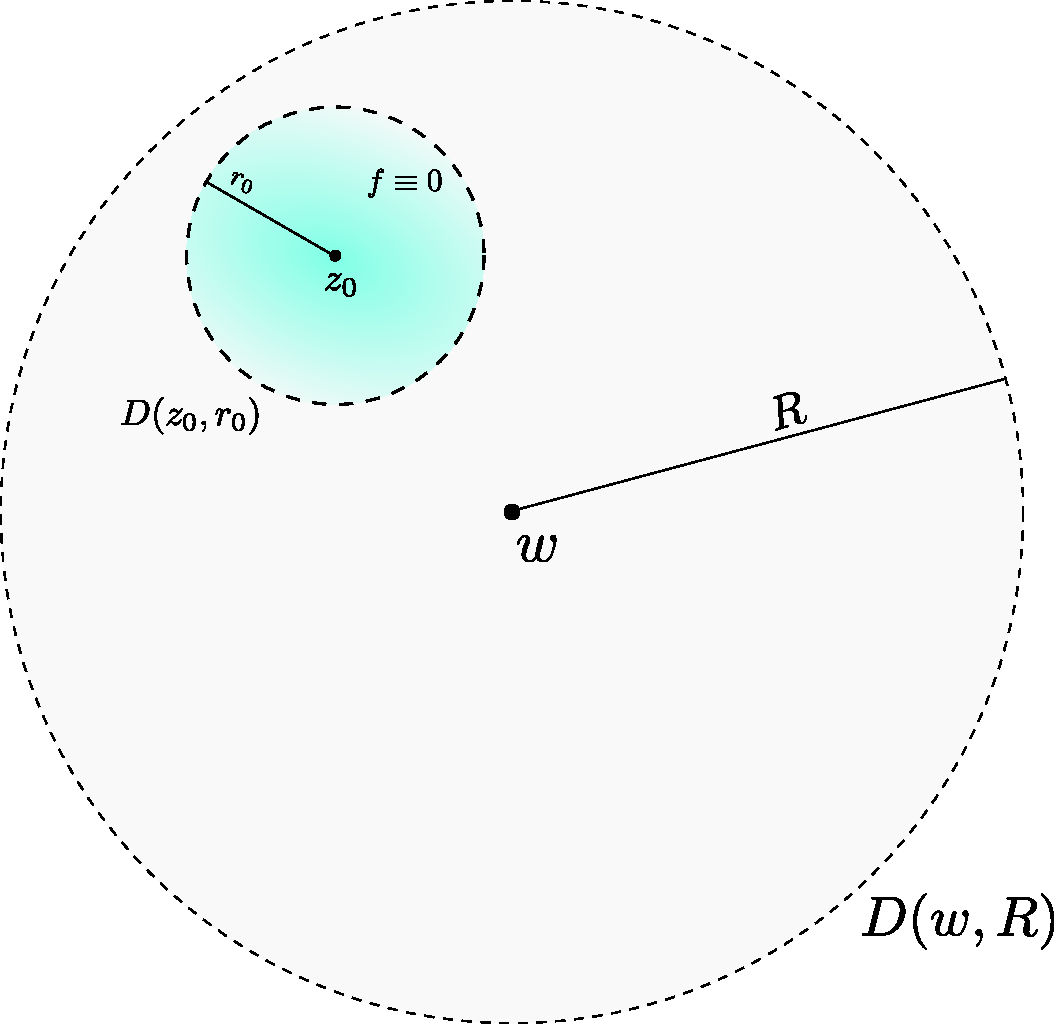
\includegraphics[width=0.6\linewidth]{Figuras/zeros-isolados2}
\caption{A função $f$ se anula em todos os pontos do disco aberto $D(z_0,r_0)$}
\label{fig:zeros-isolados2}
\end{figure}




\begin{proof}
Suponha que exista um disco aberto $D(z_0,r_0)$, com raio $r_0>0$, 
contido em $D(w,R)$ tal que $f(z)=0$ para todo $z\in D(z_0,r_0)$.
Denote por $L_{1}$ o segmento de reta unindo $z_0$ a $w$. 
Seja $z_1$ o único ponto em $L_{1}\cap \partial D(z_0,r_0)$.
Já que $f$ se anula em todos os ponto de $L_1\cap D(z_0,r_0)$ 
e $f$ é contínua em $z_1\in D(0,R)$ segue que $f(z_1)=0$. 
Ou seja, $z_1\in\mathcal{Z}(f)$. 

\begin{figure}[H]
\centering
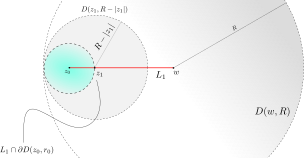
\includegraphics[width=0.6\linewidth]{Figuras/zeros-isolados3}
\caption{Construção da sequência $(z_n)_{n\in\mathbb{N}}$. O primeiro ponto da construção é mostrado acima. Ele é definido como sendo o ponto onde a reta $L_1$ intercepta o disco aberto $D(z_0,r_0)$.}
\label{fig:zeros-isolados3}
\end{figure}




Usando o Teorema \ref{teo-series-pot-analiticas} sabemos que podemos
expandir $f$ em uma série de potências, centrada em $z_1$,
e convergente em todo disco aberto $D(z_1,R-|z_1|)$,
\[
f(z) = \sum_{n=0}^{\infty}b_n(z-z_1)^n.
\]
Já que $z_1\in\mathcal{Z}(f)$ e $f\equiv 0$ em todos os pontos de $L_1$,
segue do Lema \ref{lema-centro-serie-zero-isolado} que $f\equiv 0$
em $D(z_1,R-|z_1|)$. Caso contrário $z_1$ deveria ser um zero isolado de $f$
o que é um absurdo pois $z_1$ é um ponto de acumulação de $L_1$ e 
$f$ se anula em todos os pontos de $L_1$.

 
Se $w\in D(z_1,R-|z_1|)$, não há mais nada a fazer, pois neste
caso existe um $\delta>0$ tal que $D(w,\delta)$
está contido em $D(z_1,R-|z_1|)$ 
e portanto $f\equiv 0$ em $D(w,\delta)$, 
o que implica que todos os coeficientes $a_n$'s da expansão de $f$ em torno
de $w$ são nulos. 


Caso $w\notin D(z_1,R-|z_1|)$, construímos um novo segmento de reta $L_2$
unindo $z_1$ a $w$. Seja $z_2$ o único ponto de interseção entre $L_2$
e $\partial D(z_1,R-|z_1|)$. Argumentando analogamente como acima, verificamos
que $f(z_2)=0$. Usando novamente o Lema \ref{lema-centro-serie-zero-isolado} 
podemos expandir $f$ em uma série de potências, centrada em $z_2$, 
com raio de convergência pelo menos $R-|z_2| = 2(R-|z_1|)>2(R-|z_0|)$.
Já que $z_2\in\mathcal{Z}(f)$ e $f$ se anula em todos os pontos de $L_2$
temos novamente do Lema \ref{lema-centro-serie-zero-isolado} que 
$f\equiv 0$ em $D(z_2,R-|z_2|)$. Como no caso anterior,
se $w\in D(z_2,R-|z_2|)$ não há mais nada a fazer. Caso contrário, 
repetindo os argumentos dados acima, recursivamente, 
até construirmos $z_n$ tal que 
\begin{itemize}
\item
o ponto $z_n$ é o único ponto em $\partial D(z_{n-1},R-|z_{n-1}|)\cap L_n$,
onde $L_n$ é o segmento de reta unindo $z_{n-1}$ a $w$;

\item $f\equiv 0$ em  $D(z_{n},R-|z_{n}|)$;

\item $R-|z_n|= 2^{n-1}(R-|z_1|)$;

\item  $n$ é o menor índice para o qual $w\in D(z_{n},R-|z_{n}|)$.
\end{itemize} 

O que garante a existência de um $n$ finito, satisfazendo a última condição
acima, é o crescimento exponencial obtido no penúltimo item. 

Por construção e pelos teoremas mencionados acima podemos garantir que 
$f$ é identicamente nula no disco $D(z_{n},R-|z_{n}|)$. E portanto
existe algum $\delta>0$ tal que $f$ se nula em todos
os pontos de $D(w,\delta)$. Mas isto implica que todos 
os coeficientes $a_n$'s são nulos e isto encerra a prova deste lema.
\end{proof}



\begin{teorema}[Zeros de Séries de Potência São Isolados]
\label{teo-zeros-series-isolados}
Seja $(a_n)_{n\in\mathbb{N}\cup\{0\}}$ uma sequência de números complexos
\textbf{não identicamente nula}. Suponha que a série de potências 
centrada em $z=z_0$ e gerada por esta sequência tenha raio de convergência $R>0$. 
Seja $f:D(z_0,R)\to\mathbb{C}$ a função dada por
\[
f(z) = \sum_{n=0}^{\infty}a_n(z-z_0)^n, \qquad \forall z\in D(z_0,R).
\]
Então o conjunto de zeros de $f$, notação 
$\mathcal{Z}(f)\equiv \{w\in\mathbb{C}: f(w)=0\}$,
é vazio ou formado apenas por pontos isolados. Isto é, 
para cada $z_1\in \mathcal{Z}(f)$, existe $\delta\equiv\delta_{z_1}>0$ tal que 
se $z$ satisfaz $0<|z-z_1|<\delta$ então $z\notin \mathcal{Z}(f)$.
\end{teorema}


\begin{proof}
Caso $f$ não possua zeros, não há nada a fazer. 
Logo só precisamos considerar o caso em que $\mathcal{Z}(f)$ é não-vazio. 
Seja $z_1\in\mathcal{Z}(f)$. Aplicando o Teorema \ref{teo-series-pot-analiticas}
podemos mudar o centro da série de potências de $f$ para o ponto $z=z_1$.
Obtendo assim a seguinte representação de $f$
\begin{align}\label{eq-aux-teo-zero-ser-isol}
f(z)
=
\sum_{n=0}^{\infty} b_n(z-z_1)^{n}, \qquad \forall z\in D(z_1,R_{z_1}).
\end{align}

Pelo Lema \ref{lema2-centro-serie-zero-isolado} podemos garantir 
que para algum $m\in\mathbb{N}$ temos que $b_m\neq 0$. 
De fato, se $b_n=0$ para todo $n\geqslant 0$, então $f$ é identicamente nula em $D(z_1,R_{z_1})$. Mas então segue do
Lema \ref{lema2-centro-serie-zero-isolado} que $f$ também é identicamente nula em 
$D(z_0,R)$. Portanto $a_n=0$, para todo $n\geqslant 0$ o que é uma contradição.

Já que sabemos que algum coeficiente $b_m$ em \eqref{eq-aux-teo-zero-ser-isol} é não-nulo, 
podemos aplicar o Lema \ref{lema-centro-serie-zero-isolado} e assim
garantir que $z_1$ é um zero isolado de $f$, como queríamos demonstrar.
\end{proof}


\bigskip 

\begin{definicao}[Ponto Aderente a um Conjunto]
\label{def-ponto-aderencia}
\index{Ponto!aderente}
Um ponto $z\in\mathbb{C}$ é dito um \textbf{ponto aderente} a um
conjunto $A\subset \mathbb{C}$, se existe uma sequência 
$(z_n)_{n\in\mathbb{N}}$ satisfazendo 
\begin{itemize}
\item $z_n\in A$ para todo $n\in\mathbb{N}$ (os termos da sequência são pontos de $A$);
\item $z_n\neq z_m$, se $n\neq m$ (os termos da sequência são dois-a-dois distintos);
\item $z_n\xrightarrow{\ n\to\infty\ } z$ (a sequência converge para $z$).
\end{itemize}
\end{definicao}



\begin{observacao}
Um ponto $z\in\mathbb{C}$ pode ser um ponto aderente a um conjunto 
$A\subset\mathbb{C}$, mas não ser um ponto de $A$, isto é, podemos
ter um ponto $z$ aderente a $A$ tal que $z\notin A$.

Para um exemplo simples deste caso, considere o seguinte subconjunto de $\mathbb{C}$
\[
A = \Big\{1,\frac{1}{2}, \frac{1}{3}, \frac{1}{4},\ldots\Big\}.
\]
Então é fácil ver que $0$ é aderente a $A$ mas $0\notin A$.
Outro aspecto interessante deste exemplo é que nenhum ponto do
próprio conjunto $A$ é aderente a $A$. 
\end{observacao}

\bigskip 


\begin{teorema}[Principio da Identidade]
\label{teo-principio-identidade}
\index{Principio da Identidade}
Sejam $U,V\subset \mathbb{C}$ domínios não-vazios tais que $U\cap V$ também é um domínio,
não-vazio. Sejam $f:U\to\mathbb{C}$ e $g:V\to\mathbb{C}$ duas funções analíticas. Suponha que
exista um conjunto $I\subset U\cap V$ possuindo um ponto $z_0$ aderente ao conjunto $I$, e 
tal que $f(z)=g(z)$, para todo $z\in I$. 
Então $f(z)=g(z)$ para todo $z\in U\cap V$.
\end{teorema}

\begin{figure}[H]
\centering
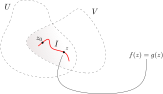
\includegraphics[width=0.65\linewidth]{Figuras/zeros-isolados4}
\caption{O conjunto $I$ onde $f$ e $g$ coincidem é marcado de vermelho. Note que nesta figura $z_0$ é um ponto aderente a $I$. Pois ele pode ser obtido como limite de uma
sequência de pontos que estão em $I$.}
\label{fig:zeros-isolados4}
\end{figure}



\begin{proof}
Vamos dividir a prova deste teorema em duas partes. A primeira parte
mostramos a validade da igualdade $f(z)=g(z)$ em um pequeno disco em torno de $z_0$.
Na segunda parte mostramos como estender a análise local, da primeira parte, 
para todo o domínio $U\cap V$. Este argumento é basicamente um argumento topológico,
mas claro, não apresentado na roupagem de topologia.


\bigskip 
Vale a pena mencionar também que a prova da primeira parte, 
seguirá diretamente dos resultados obtidos
acima, para séries de potências. E seus os argumentos são bem elementares. 
Já a segunda parte, envolve uma argumentação mais sofisticada. 
Numa primeira leitura, a prova da segunda parte pode ser omitida,
sem nenhum prejuízo à compreensão do restante do texto. 

 

\bigskip
\noindent\textbf{Parte 1.}
\\
Por hipótese $z_0\in I$ e além do mais $z_0$ é um ponto aderente a 
$I\subset U\cap V$. 
Já que $f$ e $g$ são analíticas em $U\cap V$ então podemos representar
ambas funções por séries de potências, centradas em $z_0$, com o 
raios de convergência $R_{z_0,f}$ e $R_{z_0,g}$, respectivamente.
Portanto se tomamos $R_{z_0} = \min\{R_{z_0,f},\ R_{z_0,g}\}$ temos que 
\[
f(z) = \sum_{n=0}^{\infty} a_n(z-z_0)^n
\quad \text{e}\ \quad 
g(z) = \sum_{n=0}^{\infty} b_n(z-z_0)^n,
\qquad \forall z\in D(z_0,R_{z_0}).
\]

Segue das propriedades elementares de séries de potência que a diferença das 
séries de potência acima, define uma função $h:D(z_0,R_{z_0})\to\mathbb{C}$
que é dada pela seguinte série de potências:
\[
h(z) \equiv f(z)-g(z) = \sum_{n=0}^{\infty} (a_n-b_n)(z-z_0)^n.
\]
Já que $z_0$ é um ponto aderente a $I$, existe uma 
sequência $(w_n)_{n\in\mathbb{N}}$ de pontos dois-a-dois distintos em $I$ que convergem
para $z_0$. Portanto, para algum $n_0\in\mathbb{N}$ 
temos que $w_n\in D(z_0,R_{z_0})$, para todo $n\geqslant n_0$.
Já que estamos assumindo que $f$ e $g$ coincidem em $I$
então $h(w_n)=0$ para todo $n\geqslant n_0$. 
Desta forma o conjunto de zeros de $h$, ou seja, $\mathcal{Z}(h)$
não é constituído apenas de pontos isolados, pois para todo $n\geqslant n_0$ 
temos que $w_n\in \mathcal{Z}(h)$ e $w_n\xrightarrow{\ n\to\infty\ } z_0\in \mathcal{Z}(h)$.
Logo pelo Teorema \ref{teo-zeros-series-isolados} concluímos que 
os coeficientes da expansão em série de potências de $h$, em torno de $z_0$,
são nulos. E isto mostra que $h\equiv 0$ em $D(z_0,R_{z_0})$.


\medskip
\noindent\textbf{Parte 2.}
\\
Nesta parte, vamos considerar a função $h$ da parte anterior, 
como sendo definida em todo $U\cap V$, isto é, a partir de agora 
$h:U\cap V\to\mathbb{C}$. Sua lei contínua sendo a mesma, ou seja, 
$h(z)=f(z)-g(z)$.

É óbvio que se $D(z_0,R_{z_0})\supset U\cap V$, não há mais nada a fazer. Portanto
vamos assumir que o disco aberto $D(z_0,R_{z_0})$ é um subconjunto estritamente contido
em $U\cap V$. 

%Note que das propriedades elementares de séries de potências 
%segue que $h$ é uma função analítica.
%Diferentemente da primeira parte devemos ficar atentos de que agora agora não é mais 
%possível garantir que exista algum ponto $z_1\in U\cap V$ e um 
%raio positivo $R_{z_1}$ tal que $h$, em todo
%ponto de $U\cap V$, seja representada por uma única série de potências, centrada 
%em $z_1$ com raio de convergência $R_{z_1}$. É claro que $h$ sendo uma função analítica
%ela vai admitir, em cada um dos pontos do seu domínio, uma representação por
%série de potências. Mas tanto os coeficientes quanto o raio de convergência 
%vão depender, em geral, da escolha do ponto em que centramos a série de potências, 
%que irá representar $h$.


\medskip 

Considere o conjunto de zeros da função $h$, isto é,
\[
\mathcal{Z}(h)
\equiv 
\{ z\in U\cap V : h(z)=0 \}.
\]
O objetivo é mostrar que $\mathcal{Z}(h)=U\cap V$. 
Observamos que na Parte 1, foi demonstrado que 
o disco aberto $D(z_0,R_{z_0})$ está completamente contido em $\mathcal{Z}(h)$. 

Seja $z\in U\cap V$ um ponto arbitrário. 
Como estamos supondo que $U\cap V$ é um domínio, podemos
afirmar que existe um caminho, normalizado, injetivo e suave por partes
$\gamma:[0,1]\to\mathbb{C}$ totalmente contido em $U\cap V$
cujos pontos inicial e terminal são $z_0$ e $z$, 
respectivamente. 



Sabemos que $z_0=\gamma(0)\in \mathcal{Z}(h)$ e a ideia, 
desta parte da prova, é mostrar
que $\gamma(t)$, para todo $t\in[0,1]$, está em $\mathcal{Z}(h)$.
A prova deste fato será por contradição. Vamos supor que existe ``um primeiro instante''
antes do tempo $t=1$, em que o caminho $\gamma$ deixa o conjunto de zeros de $h$. E
vamos derivar disto uma contradição.

Para formalizar esta ideia definimos
\[
t^{*} = \sup\big\{ t\in [0,1]:\, \gamma([0,t])\subset \mathcal{Z}(h) \big\}.
\]

O número $t^{*}$ pode ser pensado intuitivamente como 
o ``primeiro instante'' em que a curva $\gamma$ deixa 
o conjunto $\mathcal{Z}(h)$, embora, a rigor,
ele não seja exatamente isto.

\begin{figure}[H]
\centering
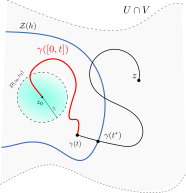
\includegraphics[width=0.55\linewidth]{Figuras/zeros-isolados5}
\caption{Esta figura ilustra a definição de $t^{*}$. A parte em vermelho corresponde a imagem por $\gamma$ do intervalo $[0,t]$ com $t<t^{*}$. Como comentado o ponto $\gamma(t^{*})$ pode ser intuitivamente pensado como o ponto onde o caminho $\gamma$ está prestes a deixar $\mathcal{Z}(h)$.}
\label{fig:zeros-isolados5}
\end{figure}





\medskip 

Na sequência, vamos usar um argumento totalmente análogo ao da Parte 1, 
para mostrar que $\gamma(t^{*})\in \mathcal{Z}(h)$ e, em
seguida, vamos concluir que $t^{*}=1$ e consequentemente que 
$z=\gamma(1)\in \mathcal{Z}(h)$.

\medskip 

Afirmamos que a continuidade de $\gamma$ implica $t^{*}>0$. 
Intuitivamente, o que esta afirmação diz é que toda a ``parte inicial'' 
do caminho $\gamma$ está contida no disco $D(z_0,R_{z_0})$, que por sua vez
está contido em $\mathcal{Z}(h)$. E portanto ``leva'' um tempo positivo para $\gamma(t)$ atingir o bordo do disco $D(z_0,R_{z_0})$. 
De forma precisa, dado $\varepsilon= R_{z_0}$,
segue da continuidade de $\gamma$ em $t=0$ que 
existe $\delta>0$ tal que se $|0-t|=|t|<\delta$ então 
$|z_0-\gamma(t)|=|\gamma(0)-\gamma(t)|<R_{z_0}$. Ou seja, 
$\gamma([0,\delta])\subset D(z_0,R_{z_0})\subset\mathcal{Z}(h)$ e 
consequentemente $0<\delta\leq t^{*}$. Na linguagem informal, usada
acima, o que mostramos é que $\gamma$ não pode deixar o conjunto $\mathcal{Z}(h)$
antes do tempo $t=\delta$. 





\medskip 




Da positividade estrita de $t^{*}$ e da definição de supremo segue 
que existe uma sequência de números positivos
distintos $(t_n)_{n\in\mathbb{N}}$ (estritamente crescente) $0<t_n< t_{n+1}<t^{*}$ tal que $t_n\to t^{*}$, quando $n\to\infty$. 
Invocando novamente a definição de supremo podemos afirmar que 
$\gamma(t_n)\in \mathcal{Z}(h)$, para todo $n\in\mathbb{N}$.
Como $h$ e $\gamma$ são funções contínuas segue que
\[
0
=
\lim_{n\to\infty} h(\gamma(t_n))
= 
h(\gamma(t^{*}))
\]
e consequentemente $\gamma(t^{*})\in\mathcal{Z}(h)$. 

Como $\gamma$ é um caminho totalmente contido em $U\cap V$ temos
que $\gamma(t^{*})\in U\cap V$. Pelo fato da função $h$ ser analítica em 
$U\cap V$, podemos representá-la por uma série de potências, centrada 
em $\gamma(t^{*})$, que converge em 
todo ponto do disco aberto $D( \gamma(t^{*}), R_{\gamma(t^{*})})$, 
com raio $R_{\gamma(t^{*})}$ positivo. 


\begin{figure}[H]
\centering
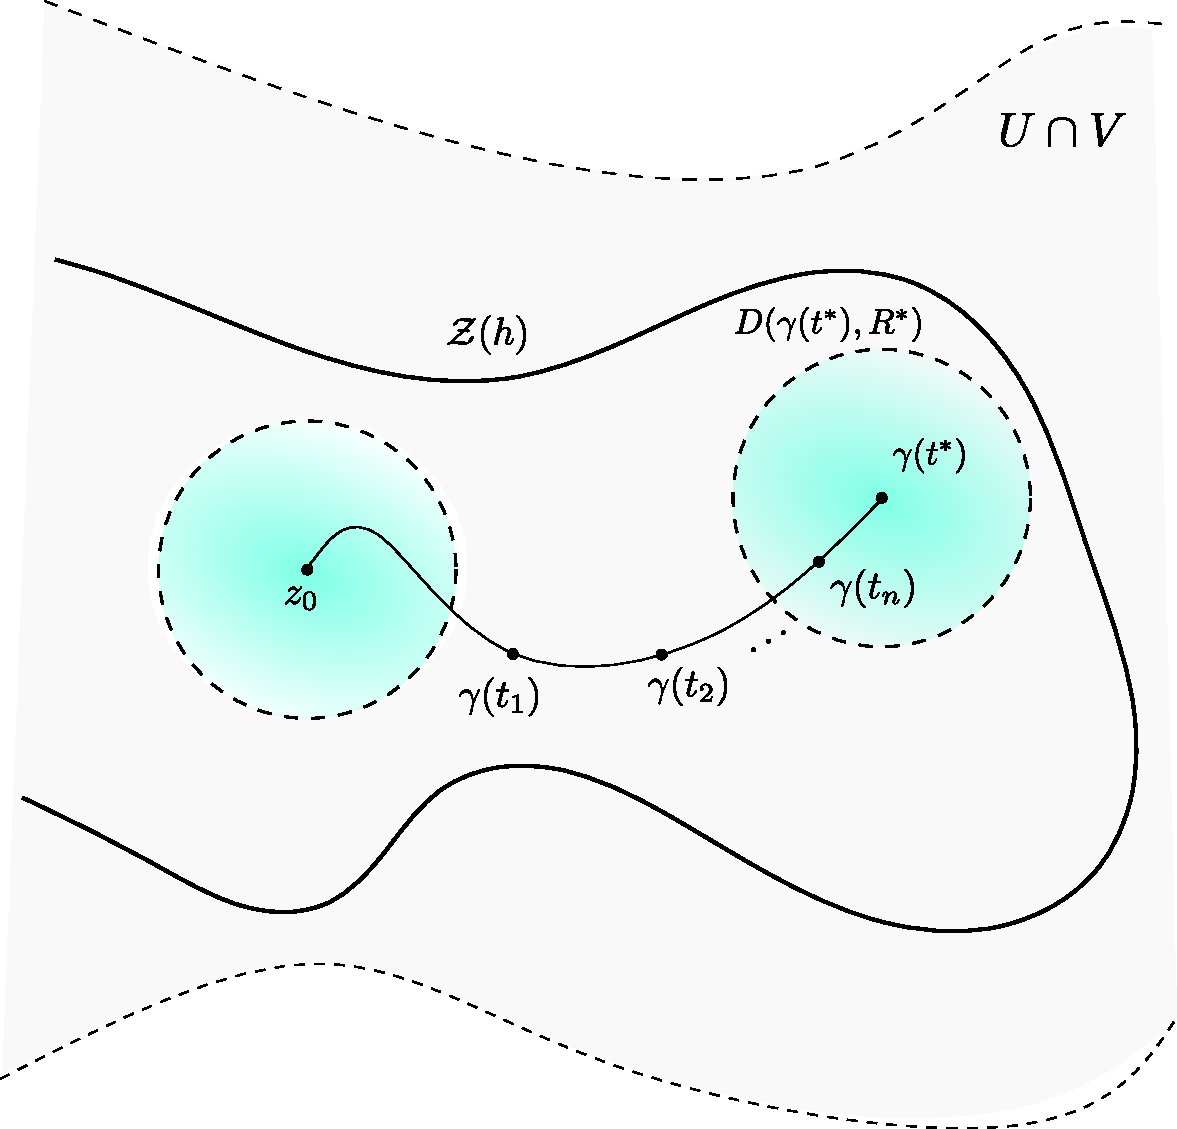
\includegraphics[width=0.6\linewidth]{Figuras/zeros-isolados6}
\caption{O disco $D(\gamma(t^{*}),R^{*})$}
\label{fig:zeros-isolados6}
\end{figure}



Já que $\gamma$ é uma curva injetiva  e $t_n<t_{n+1}$, para todo $n\in\mathbb{N}$,
então os pontos da sequência $(\gamma(t_n))_{n\in\mathbb{N}}$ são todos
distintos. Como $\gamma(t_n)\to \gamma(t^{*})$ temos que $\gamma(t^{*})$
é um ponto aderente ao conjunto $\widetilde{I}\equiv \{\gamma(t^{*}),\gamma(t_1),\gamma(t_2),\ldots\}$.

Argumentando analogamente como na Parte 1, apenas substituindo $I$ por $\widetilde{I}$ 
podemos mostrar que existe algum $R^*>0$ tal que $h\equiv 0$
no disco $D(\gamma(t^*),R^{*})$ e consequentemente que 
$D(\gamma(t^*),R^{*})\subset\mathcal{Z}(h)$.

\medskip 


Depois de todos este preparativos, estamos finalmente prontos para provar que $t^{*}=1$.
De fato, suponha por contradição que $t^{*}<1$. 
Escolhido $\varepsilon = R^{*}$, segue da continuidade de $\gamma$ que 
existe $\delta$ satisfazendo $0<\delta<1-t^{*}$ tal que se $|t-t^{*}|<\delta$ então 
$|\gamma(t)-\gamma(t^{*})|<R^{*}$. Portanto, segue das propriedades
elementares de função ($F(A\cup B)=F(A)\cup F(B)$), da definição de $t^{*}$, 
do argumento de continuidade deste parágrafo e da continência 
$D(\gamma(t^*),R^{*})\subset\mathcal{Z}(h)$
(estabelecida no parágrafo anterior), que 
\begin{align*}
\gamma([0,t^{*}+\delta/2])
=
\gamma([0,t^{*}])\cup \gamma([t^{*},t^{*}+\delta/2])
\subset \mathcal{Z}(h)\cup D(\gamma(t^*),R^{*})
=
\mathcal{Z}(h),
\end{align*}
o que é uma contradição com a definição de $t^{*}$. Como mostramos que $t^{*}$ não pode ser nenhum dos pontos do intervalo $[0,1)$, só resta $t^{*}=1$. Disto segue 
finalmente que $z\in \mathcal{Z}(h)$. Como $z$ foi 
escolhido arbitrariamente em $U\cap V$ segue que $\mathcal{Z}(h)=U\cap V$
e o teorema está finalmente demonstrado.
\end{proof}





\begin{corolario}[Unicidade de Extensões Analíticas]
\label{cor-unicidade-ext-analiticas}
\index{Extensão!analítica}
Sejam $U,V\subset \mathbb{C}$ domínios não vazios, com $U$ estritamente contido em $V$. 
Seja $f:U\to\mathbb{C}$ uma função analítica. Se $F:V\to\mathbb{C}$
e $G:V\to\mathbb{C}$ são funções analíticas que estendem $f$ (extensões
analíticas de $f$), isto é, $F|_{U}=f=G|_{U}$, então $F=G$. 
\end{corolario}


\begin{proof}
A ideia é aplicar o  Teorema \ref{teo-principio-identidade} às funções $F$ e $G$.
Para isto vamos mostrar que todas as hipóteses deste teorema são satisfeitas. 

Primeiro, o teorema citado acima, 
exige que $F$ e $G$ sejam funções analíticas definidas em domínios não-vazios, 
o que é o caso aqui. Ele também exige que $\mathrm{dom}(F)\cap\mathrm{dom}(G)$
seja um domínio não-vazio. Neste caso, esta interseção é precisamente o conjunto $U$,
que por hipótese, é um domínio não-vazio.
Além disto deve, existir um conjunto $I\subset \mathrm{dom}(F)\cap\mathrm{dom}(G)$
possuindo um ponto $z_0$ aderente a $I$, onde $F$ e $G$ coincidem. Neste 
caso o conjunto $I$ pode ser tomado como $I=U=\mathrm{dom}(f)$. De fato,
como $U$ é um domínio não-vazio, dado qualquer ponto $z_0\in U$ 
podemos encontrar um raio $r>0$, tal que que o disco aberto $D(z_0,r)\subset U$.
Logo $z_0$ é um ponto aderente a $U$. Como $F$ e $G$ são extensões de $f$, 
então temos que $F$ e $G$ coincidem em $U$.

Portanto, todas as hipóteses do Teorema 
\ref{teo-principio-identidade} estão garantidas. 
Então ele afirma que $F$ e $G$ coincidem 
em $\mathrm{dom}(F)\cap\mathrm{dom}(G)= V$, e logo $F=G$,
como queríamos demonstrar.
\end{proof}






\begin{exemplo}
Considere a seguinte identidade, bem conhecida, para todo $x,y\in\mathbb{R}$
\begin{align}\label{eq-aux1-form-prod-exp-ext-analitica}
\sum_{n=0}^{\infty} \frac{(x+y)^n }{n!}
=
e^{x+y}
=
e^xe^y
= 
\left( \sum_{n=0}^{\infty} \frac{x^n}{n!} \right)
\left( \sum_{n=0}^{\infty} \frac{y^n}{n!} \right).
\end{align}

Vamos mostrar como as técnicas de extensões analíticas 
(Teorema \ref{teo-principio-identidade})
podem ser usadas para estender a identidade acima para números complexos, isto é,
\[
\sum_{n=0}^{\infty} \frac{(z+w)^n }{n!}
= 
\left( \sum_{n=0}^{\infty} \frac{z^n}{n!} \right)
\left( \sum_{n=0}^{\infty} \frac{w^n}{n!} \right),
\qquad \forall z,w\in\mathbb{C}.
\]

Primeiro, observamos que todas as séries que aparecem acima são convergentes. 
Na verdade, a série de potências dada por
\[
f(z) = \sum_{n=0}^{\infty} \frac{z^n}{n!}
\]
tem raio de convergência
\[
R 
= 
\frac{1}{\displaystyle  \limsup_{n\to\infty} \sqrt[n]{ \frac{1}{n!} } }
=
\limsup_{n\to\infty} \sqrt[n]{ n! }
=+\infty
\]


Fixe $w\in \mathbb{R}$ e considere as funções 
$f_{w}:\mathbb{C}\to\mathbb{C}$ e $g_{w}:\mathbb{C}\to\mathbb{C}$ 
dadas por 
\begin{align*}
f_{w}(z) = \sum_{n=0}^{\infty} \frac{(z+w)^n }{n!}
\quad\text{e}\quad
g_{w}(z) = \left( \sum_{n=0}^{\infty} \frac{z^n}{n!} \right)
\left( \sum_{n=0}^{\infty} \frac{w^n}{n!} \right),
\qquad \forall z\in\mathbb{C}.
\end{align*}

Pelo Teorema \ref{teo-series-pot-analiticas} e pela observação anterior 
é claro que ambas, são funções analíticas
definidas em $\mathbb{C}$. 
Seguindo a notação do Teorema \ref{teo-principio-identidade},
note que se tomamos $I=\mathbb{R}\subset \mathbb{C}$, 
então temos, por exemplo, que $0$ é aderente a $I$ 
e além do mais, para todo $z\in I$, temos que
$f_{w}(z)=g_{w}(z)$. 


\begin{figure}[H]
\centering
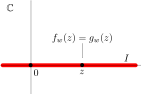
\includegraphics[width=0.4\linewidth]{Figuras/zeros-isolados7}
\caption{Para $z\in\mathbb{R}$ temos que $f_{w}(z)=g_{w}(z)$.}
\label{fig:zeros-isolados7}
\end{figure}



De fato, como $w$ e $z$ são reais e esta igualdade segue imediatamente
de \eqref{eq-aux1-form-prod-exp-ext-analitica}.
Portanto podemos aplicar o  Teorema \ref{teo-principio-identidade}. 
Neste caso ele garante que a igualdade
permanece válida em todo os pontos da interseção dos domínios das funções $f_{w}$ e 
$g_{w}$. Mas como ambas estão definidas em todo plano complexo segue que
$f_{w}(z)=g_{w}(z)$, para todo $z\in \mathbb{C}$. Portanto temos
\begin{align}\label{eq-aux2-form-prod-exp-ext-analitica}
\sum_{n=0}^{\infty} \frac{(z+w)^n }{n!}
=
\left( \sum_{n=0}^{\infty} \frac{z^n}{n!} \right)
\left( \sum_{n=0}^{\infty} \frac{w^n}{n!} \right),
\qquad \forall z\in\mathbb{C} \ \text{e}\ w\in\mathbb{R}.
\end{align}

Para completar a prova da identidade, 
precisamos de mais um passo. Permitir que $w$ seja também
qualquer número complexo. Mas a ideia é a mesma, porém 
agora podemos contar com a vantagem de poder construir as ``funções auxiliares'''
$f_{w}$ e $g_{w}$, fixando números complexos! 

\medskip 

Fixe um número complexo arbitrário $z\in \mathbb{C}$. 
Como o Teorema \ref{teo-series-pot-analiticas}
permite afirmar que qualquer série de potências define em seu raio de convergência
uma função analítica. As seguintes 
funções $F_{z}:\mathbb{C}\to\mathbb{C}$ 
e $G_{z}:\mathbb{C}\to\mathbb{C}$ dadas por 
\[
F_z(w) = \sum_{n=0}^{\infty} \frac{(z+w)^n }{n!}
\quad\text{e}\quad
G_z(w) = 
\left( \sum_{n=0}^{\infty} \frac{z^n}{n!} \right)
\left( \sum_{n=0}^{\infty} \frac{w^n}{n!} \right),
\qquad \forall w\in\mathbb{C}.
\]
são funções analíticas. Repare que $F_z$ deve ser vista como uma série de potências, centrada em $z$, e $G_{z}$ como uma série de potências centrada em zero multiplicada
por uma constante. 


Considerando novamente $I=\mathbb{R}\subset \mathbb{C}$, 
e $0$ como ponto aderente a $I$ temos de 
\eqref{eq-aux2-form-prod-exp-ext-analitica} que 
$
F_{z}(w)=G_{z}(w)
$
para todo $w\in I$. 
Aplicando novamente o Teorema \ref{teo-principio-identidade},
concluímos que $F_{z}(w)=F_{z}(w)$ para todo $w\in\mathbb{C}$. 
Como $z$ é arbitrário podemos afirmar que vale então a seguinte
identidade: 

\begin{align}\label{eq-aux3-form-prod-exp-ext-analitica}
\sum_{n=0}^{\infty} \frac{(z+w)^n }{n!}
=
\left( \sum_{n=0}^{\infty} \frac{z^n}{n!} \right)
\left( \sum_{n=0}^{\infty} \frac{w^n}{n!} \right),
\qquad \forall z,w\in\mathbb{C}.
\end{align}






\medskip 
\noindent
\textbf{Observação}. Apesar deste exercício usar um exemplo simples para
mostrar como se aplicam as técnicas de extensão analíticas, 
só faz sentido ter escolhido este e não outro, 
porque ainda não provamos que a exponencial complexa, definida 
anteriormente por, $\exp(z)\equiv e^{x}(\cos(y)+i\sen(y))$, onde $z=x+iy$,
admite a representação por sua série de Taylor 
\[
\exp(z) = \sum_{n=0}^{\infty} \frac{z^n}{n!}, \qquad \forall z\in\mathbb{C}.
\]
Um roteiro para prova deste fato é apresentado na lista de exercícios. 
Também daremos, mais a frente, outra prova deste fato no texto, após apresentarmos 
a Fórmula Integral de Cauchy.
\end{exemplo}







\begin{exemplo}
Um dos exemplos mais instrutivos sobre extensões analíticas é dado pela 
série geométrica. Como sabemos a série geométrica em $\mathbb{C}$ pode ser 
vista como uma série de potências, centrada em zero e de raio de convergência $R=1$.
Esta série define uma função analítica $f:\mathbb{D}\to\mathbb{C}$ dada por 
\[
f(z) = \sum_{n=0}^{\infty} z^n.
\]
Por outro lado, considere a 
função $g:\mathbb{C}\setminus\{1\}\to\mathbb{C}$ dada por
\[
g(z) = \frac{1}{1-z}.
\]

Também sabemos que
\[
f(z) = \sum_{n=0}^{\infty}z^n  = \frac{1}{1-z} = g(z), \qquad \forall z\in\mathbb{D}.
\]

Em outras palavras, a igualdade acima diz que $f=g|_{\mathbb{D}}$. 
Ou seja, $g$ é uma extensão de $f$. Procedendo analogamente ao Exemplo \ref{exe-1/z-analitica} podemos
mostrar sem dificuldades que a função 
$g:\mathbb{C}\setminus\{1\}\to\mathbb{C}$ é analítica. 
Então o que a igualdade acima nos diz é que $f$ admite uma 
(única - Corolário \ref{cor-unicidade-ext-analiticas}) 
extensão analítica à $\mathbb{C}\setminus\{1\}$. 

Obviamente podemos calcular $g(3)$, substituindo o número complexo $3$ na 
expressão $1/(1-z)$, pois $3$ é um ponto do domínio de $g$. 
Mas apesar de $g$ ser uma extensão de $f$, \textbf{não} faz nenhum sentido
falar em $f(3)$ muito menos escrever 
\[
\sum_{n=0}^{\infty} 3^n = f(3) = g(3) = -\frac{1}{2}.
\]

Este tipo de confusão geralmente é causado pelo frequente abuso de notação
de denotar $f$ e sua extensão pelo mesmo símbolo. Esta não é uma prática
ruim, mas devemos ter sempre em mente que dependendo do ponto em que vamos
calcular a extensão, devemos ser cuidadosos e não 
usar a expressão algébrica da função $f$ inicialmente dada.
Compreender precisamente esta diferença é ainda mais fundamental
para lidar com casos onde a extensão é obtida por algum 
argumento abstrato de existência. Vamos discutir este assunto
mais profundamente e apresentar outros exemplo mais à frente.
\end{exemplo}


\begin{observacao}
No exemplo acima mostramos que $f:\mathbb{D}\to\mathbb{C}$ dada por
\[
f(z) = \sum_{n=0}^{\infty} z^n, \qquad \forall z\in\mathbb{D}
\]
admite uma extensão analíticas à $\mathbb{C}\setminus\{1\}$.
Isto é, 
\[
\sum_{n=0}^{\infty} z^n = \frac{1}{1-z}, \qquad \forall z\in \mathbb{D}.
\]
Por outro lado, vimos no Exemplo \ref{exemplo-divergencia-bordo-disc-conv}
que a série acima diverge para todo $z_0\in \partial\mathbb{D}$. 
Mas observe que para todo 
$z\in \partial\mathbb{D}\setminus\{1\}$ a função $g$ é contínua em todo
$\mathbb{C}\setminus\{1\}$.
Em particular, se $z_0\in\partial\mathbb{D}\setminus\{1\}$ temos
\[
\lim_{z\to z_0}g(z) = \lim_{z\to z_0}\frac{1}{1-z} = \frac{1}{1-z_0}=g(z_0).
\]
Logo o limite acima existe por qualquer caminho. Então podemos tomá-lo
por pontos que estão no interior do disco unitário. 
Dentro do disco unitário sabemos que 
$f=g$, logo temos 
\[
\frac{1}{1-z_0}
=
g(z_0)
=
\lim_{ \substack{z\to z_0 \\ z\in\mathbb{D}\  }  }\ g(z)
=
\lim_{ \substack{z\to z_0 \\ z\in\mathbb{D}\  }  }\ f(z)
=
\lim_{ \substack{z\to z_0 \\ z\in\mathbb{D}\  }  }\ \sum_{n=0}^{\infty} z^n.
\]
Todas as igualdades acima são realmente válidas. 
Mas por que, já que $g$ é um extensão analítica (portanto contínua) de $f$,
agora não temos uma contradição com o fato da série $\sum_{n=0}^{\infty} z^n$
divergir em $z_0$ e ao mesmo tempo $g(z_0)$ estar bem definido? Isto é, 
o que tem de errado em concluir da igualdade acima (absolutamente correta) que
\[
\text{bem definido} \ \longrightarrow  \ g(z_0) = \sum_{n=0}^{\infty}z_0^n
\ \longleftarrow \ \text{diverge}. 
\]

Refraseando a pergunta. Por que a existência de uma extensão analítica para
a série $\sum_{n=0}^{\infty} z^n$, à todo $\mathbb{C}\setminus\{1\}$, em particular, 
à todo disco unitário, exceto $z=1$ não conflita com o fato da 
série ser divergente em todo ponto do bordo do disco unitário?
\end{observacao}

%\chapter*{Lista 5}
\addcontentsline{toc}{chapter}{Lista 5}
\markboth{Lista 5}{Lista 5}
%%%%%%%%%%%%%%%%%%%%%%%%%%%%%%%%%%%%%%%%%%%%%%%%



% Inicio da Lista de Exercícios 
\begin{enumerate}[leftmargin=*]


	\item Calcule $\displaystyle \lim_{n\to\infty} \frac{n!}{n^n}$.

	\item Mostre que, se $|\alpha|<1$ então $\displaystyle\lim_{n\to\infty}n\alpha^n=0$.

	\item Calcule $\displaystyle \lim_{n\to\infty}\left[i+\left(\frac{2+3i}{5}\right)^n \right]$.

	\item Existe o seguinte limite: $\displaystyle \lim_{n\to\infty}\left[i+\left(\frac{2+3i}{5}\right)^n \right]$ ?



	\item Calcule
		\begin{eqnarray*}
			\lim_{n\to\infty} \frac{\log n}{n},
			&\qquad\displaystyle\lim_{n\to\infty} \sqrt[n]{n},	
			&\qquad\lim_{n\to\infty}\frac{\log(ni)}{ni}
			%
			\\[0.3cm]
			%
			\lim_{n\to\infty} \sqrt[n]{ni},
			&\qquad\displaystyle\lim_{n\to\infty} \sqrt[ni]{ni},		
			&\qquad\lim_{n\to\infty} \sqrt[ni]{n}.
		\end{eqnarray*}
		
	\item Para cada $\alpha\in\mathbb{C}$ diga se cada uma das sequências converge ou diverge e, 
			se convergir, determine o limite:
			$$
			\begin{array}{llll}
				\alpha^n,
				&\qquad\displaystyle n\alpha^n,	
				&\qquad\displaystyle \frac{\alpha^n}{n}
				&\qquad\displaystyle \sqrt{n}\left(\sqrt{n+\alpha}-\sqrt{n}\right)
			\end{array}	
			$$
 
 	\item Suponha que $|\alpha|<|\beta|<1$. Existe o limite $\displaystyle \sqrt[n]{\alpha^n+\beta^n}$ ?
 
 	\item Suponha que $1<|\alpha|=|\beta|$. Mostre que, se a sequência $\alpha^n-\beta^n$ 
 		é limitada, então $\alpha=\beta$.

 	\item Existem os seguintes limites: 
 			$$
			\begin{array}{lll}
				\displaystyle \lim_{n\to\infty} \cos(n\pi i)
				&\qquad\text{e}
				&\qquad\displaystyle \lim_{n\to\infty} ni\,\text{sen}\left(\frac{\pi i}{n}\right) ?	
			\end{array}	
			$$

	\item Mostre que as séries abaixo divergem
			$$
			\begin{array}{lll}
				\displaystyle \sum_{n=1}^{\infty}\frac{1}{ni}
				&\qquad\text{e}
				&\qquad\displaystyle \sum_{n=1}^{\infty}\frac{1}{n+i}.
			\end{array}	
			$$

	\item Determine o raio de convergência de cada uma das séries abaixo:
	 \begin{equation*}
		\begin{array}{llll}
			&\displaystyle\sum_{n=0}^{\infty}\frac{n}{(3i)^n}(z-1)^n,
			&\qquad \displaystyle \sum_{n=0}^{\infty}\frac{11^{n+2i}}{n!} z^n,
			&\qquad \displaystyle \sum_{n=0}^{\infty}\frac{n^{2i}}{2^n} (z-\pi)^n,
			%
			\\[1.0cm]
			%
			&\displaystyle\sum_{n=0}^{\infty} \frac{5}{(4+3i)^n} z^n,
			&\qquad \displaystyle \sum_{n=0}^{\infty} \frac{7n}{(5+i)^n} (z+2)^n,
			&\qquad \displaystyle \sum_{n=1}^{\infty} \frac{1}{\log (ni)} z^n,
			%
			\\[1.0cm]
			%
			&\displaystyle\sum_{n=0}^{\infty}\frac{i^n}{2^{ni}}z^n,
			&\qquad \displaystyle \sum_{n=1}^{\infty} \frac{(-1)^{n+1}}{n\sqrt{3i}} z^n,
			&\qquad \displaystyle \sum_{n=0}^{\infty} \frac{3^{ni}}{i(2n)!} z^n,
			%
			\\[1.0cm]
			%
			&\displaystyle\sum_{n=0}^{\infty}\frac{(n!)^2}{(2n)!}z^n,
			&\qquad \displaystyle \sum_{n=1}^{\infty} \left(1+\frac{1}{n}\right)^n z^n,
			&\qquad \displaystyle \sum_{n=1}^{\infty} \left(1+\frac{1}{n}\right)^{n^2} z^n,
			%
			\\[1.0cm]
			%
			&\displaystyle\sum_{n=1}^{\infty} \left(1-\frac{1}{n}\right)^n z^n,
			&\qquad \displaystyle \sum_{n=1}^{\infty} n^{\log n} z^n,
			&\qquad \displaystyle \sum_{n=1}^{\infty} \frac{1}{(\log n)^n} z^n,
		\end{array}
	 \end{equation*}	

	\item Mostre usando o produto de séries que se $f(z)=\displaystyle\sum_{n=0}^{\infty}a_n z^n$
	então
	$$
	\frac{1}{1-z}f(z) = \sum_{n=0}^{\infty}(a_0+\ldots+a_n)z^n.
	$$
	
	\item Mostre que 
		\begin{itemize}
		\item $\displaystyle \sum_{n=0}^{\infty} (n+1)z^n =\frac{1}{(1-z)^2}$.
		\item $\displaystyle \sum_{n=1}^{\infty} nz^n =\frac{z}{(1-z)^2}$.
		\item $\displaystyle \sum_{n=1}^{\infty} n^2z^n =\frac{z+z^2}{(1-z)^2}$.
		\item $\displaystyle \sum_{n=1}^{\infty} n^3z^n =\frac{z+4z^2+z^3}{(1-z)^4}$.
		\item $\displaystyle \sum_{n=1}^{\infty} n^4z^n =\frac{z+11z^2+11z^3+z^4}{(1-z)^5}$.
		\end{itemize}
	
	\item Seja $P(t)=a_0+a_1t+\ldots+a_kt^k$ um polinômio e considere a sequência 
			$\{P(n)\}_{n\in\mathbb{N}}$. Então 
			$$
				f(z) = \sum_{n=1}^{\infty} P(n)z^n
			$$
		é uma função racional. \\
		{\bf Dica:} comece considerando monômios, isto é, séries da forma $\sum_{n=0}^{\infty}n^kz^n$.
		Para estes casos inspiri-se no exercício anterior.
		
	
	\item Considere uma série de potências $\sum_{n=0}^{\infty}a_nz^n$ 
		na qual os coeficientes se repetem ciclicamente, $a_{n+k}=a_{n}$,
		onde $n$ é qualquer e $k$ um inteiro positivo fixado. Calcule
		seu raio de convergência e sua soma.


	\item Seja 
	$$
		f(z) = 1+\sum_{n=1}^{\infty} \frac{\alpha(\alpha-1)\ldots(\alpha-n+1)}{n!}\ \ z^n,
		\qquad\text{onde}\ \alpha\in\mathbb{R}. 
	$$
	Mostre que $f$ converge para todo $|z|<1$ e que $f'(z)=\frac{\alpha f(z)}{1+z}$. 
	Conclua daí que $[(1+z)^{\alpha}f(z)]'=0$ e que $f(z)=(1+z)^{\alpha}$. 
	Este resultado pode ser generalizado para $\alpha\in\mathbb{C}$ ?
		


	\item Use os resultados do apêndice sobre o raio de convergência, do livro texto, 
		para calcular o raio de convergência das seguintes séries:
		\begin{itemize}
			\item $\displaystyle \sum_{n=0}^{\infty}\frac{(n!)^2}{(2n)!}\, z^{2n}$.
			\item $\displaystyle \sum_{n=1}^{\infty}\left( 1+ \frac{1}{n}\right)^{n} z^{n^2}$.
			\item $\displaystyle \sum_{n=1}^{\infty}\left( 1+ \frac{1}{n}\right)^{n^2} z^{n^2}$.
		\end{itemize}		 

	
\end{enumerate}

% Semana 6
%% !TeX spellcheck = pt_BR
\chapter[Semana 6]{}
\chaptermark{}


\hfill%
\begin{minipage}{12cm}
	\begin{flushright}
		\rightskip=0.5cm
		\textit{``At the basis of the distance concept lies, for example, 
		the concept of a convergent point sequence and their defined limits,
		and one can, choosing these ideas as those fundamental to the point 
		set theory, eliminate the notions of distance ... Thirdly, 
		we can associate with each point of the set certain parts of the space
		called neighborhoods, and these can again be made building stones of the 
		theory with the elimination of the distance concept. Here the view
		of a set is in consideration of the association between elements and
		subsets.''}
		\\[0.1cm]
		\rightskip=0.5cm
		---F. Hausdorff, 1949
	\end{flushright}
\end{minipage}



\section[Diferenciabilidade Complexa de Séries de Potências]
{Diferenciabilidade Complexa de Séries\\ de Potências}
\begin{center}
Em construção...
\end{center}




\section[Princípio da Identidade para Séries de Potências]
{Princípio da Identidade para Séries\\ de Potências}
\begin{center}
Em construção...
\end{center}




% Semana 7 
% !TeX spellcheck = pt_BR
%\chapter[Semana 7]{}
\chapter[Teoria de Cauchy]{Teoria de Cauchy:\\ Integração no plano complexo}
\chaptermark{}


\hfill%
\begin{minipage}{12cm}
	\begin{flushright}
		\rightskip=0.5cm
		\textit{``At the basis of the distance concept lies, for example, 
		the concept of a convergent point sequence and their defined limits,
		and one can, choosing these ideas as those fundamental to the point 
		set theory, eliminate the notions of distance ... Thirdly, 
		we can associate with each point of the set certain parts of the space
		called neighborhoods, and these can again be made building stones of the 
		theory with the elimination of the distance concept. Here the view
		of a set is in consideration of the association between elements and
		subsets.''}
		\\[0.1cm]
		\rightskip=0.5cm
		---F. Hausdorff, 1949
	\end{flushright}
\end{minipage}



\section{A Integral Complexa}

\begin{lema}
Sejam $U \subset \C$ um domínio e $f:U \to \C$ uma função holomorfa. Se $f'(z) = 0$ para
todo ponto $z\in U$, então $f$ é uma função constante.
\end{lema}

\begin{definicao}[Integral complexa]
\label{def:integral-complexa}
\index{Integral complexa}
A integral da função $f$ ao longo do caminho $\y$ é
o número complexo
\begin{equation*}
    \int_{\y} f(z) dz = \int_a^b f(\y(t))\y'(t) dt,
\end{equation*}
sendo $\y:[a,b]\to\C$ um caminho suave e
$f:U \to \C$ função contínua com $U$ domínio.
\end{definicao}

\begin{definicao}
Sejam $f$ e $U$ como na Definição \ref{def:integral-complexa} e
$\y = \y_1*\y_2*\cdots*\y_n$ um caminho suave por partes em $U$.
A integral de $f(z)$ ao longo de $\y$ é o número complexo
\begin{equation*}
    \int_{\y} f(z)dz = \sum_{i=1}^n\int_{\y_i} f(z)dz.
\end{equation*}
\end{definicao}



\section[Primitivas e o Teorema Fundamental do Cálculo]
{Primitivas e o Teorema Fundamental\\ do Cálculo}

\begin{definicao}
\label{def:primitiva-complexa}
Seja $f:U \to \C$ uma função contínua com $U\subset\C$ domínio. Uma função $F:U\to\C$
é chamada primitiva de $f$ se $F$ é holomorfa em $U$ e $F'(z) = f(z), \forall z\in U$.
\end{definicao}

\begin{teorema}

Sejam $U\subset\C$ domínio, $f:U\to\C$ função contínua,
$F$ uma primitiva de $f$ em $U$ e $\y$ um caminho suave por partes em $U$ unindo $z_0$ a $z_1$. Então
\begin{equation*}
    \int_{\y} f(z)dz = F(z_1) - F(z_0).
\end{equation*}
Em particular, se o caminho é fechado então
\begin{equation*}
    \int_{\y} f(z)dz = 0.
\end{equation*}
\end{teorema}

\begin{proposicao}
Seja $\displaystyle{ f(z) = \sum_{n=0}^{\infty} a_n(z-z_0)^n }$
definida por uma série de potências com raio de convergência $R>0$.
Então a função
\begin{equation*}
    F(z) = \sum_{n=0}^{\infty} \frac{a_n}{n+1}(z-z_0)^{n+1}
\end{equation*}
é uma primitiva de $f$ e a série que a define converge para $|z-z_0| < R$.
\end{proposicao}

\begin{lema}[Lema Técnico]
\label{lema-tecnico}
Sejam $U\subset\C$ um domínio, $f:U\to\C$ uma função contínua e
$\y(t), a\leq t\leq b$ um caminho suave por partes em $U$, de comprimento $l(\y)$.
Seja $K\geq 0$ um número real tal que $|f(\y(t))| \leq K$ para todo $a\leq t\leq b$. Então
\begin{equation*}
    \left| \int_{\y}f(z)dz \right| \leq Kl(\y).
\end{equation*}
\end{lema}

\begin{teorema}
Seja $f:U\to \C$ uma função contínua definida no domínio $U\subset\C$. As seguintes afirmações são equivalentes:
\begin{enumerate}[(i)]
    \item $f$ tem uma primitiva em $U$
    \item $\int_{\y} f(z) dz = 0$ para qualquer caminho $\y$ fechado e suave por partes em $U$.
    \item $\int_{\lambda} f(z) dz$ só depende dos pontos inicial e final de qualquer caminho $\lambda$ suave por partes em $U$.
\end{enumerate}
\end{teorema}


\section[Os teoremas de Cauchy]{Os teoremas de Cauchy}

\begin{teorema}[Teorema de Cauchy-Goursat]
\label{teo:cauchy-goursat}
\index{Teorema!de Cauchy-Goursat}
Sejam $U$ um domínio em $\C$ e $f: U \to \C$ uma função holomorfa. Suponha que $\Delta \subset U$ é uma triângulo que limita
uma região inteiramente contida em $U$. Então
\begin{equation*}
    \int_{\Delta} f(z) dz = 0.
\end{equation*}
\end{teorema}


\begin{definicao}[Domínio estrelado]
\index{Domínio estrelado}
Seja $U\subset\C$ um domínio. Dizemos que $U$ é estrelado se existe um ponto $z_0\in U$
tal que dado qualquer ponto $z\in U$, o segmento de reta $\overline{z_0z}$ está inteiramente contido em $U$. 
O ponto $z_0$ é chamado um centro do domínio $U$.
\end{definicao}


\begin{corolario}
Sejam $U\subset\C$ um domínio estrelado e $f:U\to\C$ uma
função holomorfa. Então $f$ admite uma primitiva em $U$.
\end{corolario}


\begin{corolario}[Teorema de Cauchy-Goursat bis]
Sejam $U\subset\C$ um domínio estrelado e $f:U\to\C$ uma função holomorfa.
Se $\y$ é um caminho fechado suave por partes em $U$, então
\begin{equation*}
    \int_{\y} f(z) dz = 0.
\end{equation*}
\end{corolario}


\begin{teorema}[Fórmula Integral de Cauchy]
\label{teo:form-integral-cauchy}
\index{Fórmula Integral de Cauchy}
Seja $f:U \to \C$ uma função holomorfa definida no domínio $U\subset\C$.
Sejam $\overline{D}(z_0, r_0)$ um disco fechado inteiramente contido em $U$ e $\y$ sua fronteira, orientada compativelmente. 
Se $z$ é um ponto qualquer no interior de $\overline{D}(z_0, r_0)$ então
\begin{equation*}
    f(z) = \frac{1}{2\pi i}\int_{\y} \frac{f(w)}{w-z}dw.
\end{equation*}
\end{teorema}


\begin{corolario}
Seja $f:U\to\C$ holomorfa com $U$ domínio. Então $f$ tem derivadas de todas as ordens em todos os pontos de $U$ e
\begin{equation*}
    f^{(n)}(z) = \frac{n!}{2\pi i}\int_{\y} \frac{f(w)}{(w-z)^{n+1}}dw, \forall z\in U,
\end{equation*}
onde $\y$ é qualquer circunferência centrada em $z$, percorrida no sentido anti-horário e limitando um disco fechado contido em $U$.
\end{corolario}


\begin{corolario}[Estimativas de Cauchy]
\label{cor-estimativas-cauchy}
\index{Estimativas de Cauchy}
Seja $f$ uma função holomorfa definida no disco $D(z_0, R)$ e suponha que
$|f|\leq K$ em $D(z_0, R)$. Então
\begin{equation*}
    |f^{(n)}(z_0)| \leq \frac{n!K}{R^n}.
\end{equation*}
\end{corolario}


\begin{corolario}[Teorema de Liouville]
\label{teo-liouville}
\index{Teorema!de Liouville}
Seja $f$ função inteira. Se existe $K\geq 0$ tal que $|f(z)|\leq K$ então $f$ é uma função constante.
\end{corolario}


\begin{lema}
Seja $D(a,r), r>0$, um disco e $f: D(a,r)\to\C$ uma função holomorfa. 
Se a imagem de $f$ está contida no interior de uma circunferência $|w| - \alpha$, então $f$ é uma função constante.
\end{lema}


\begin{corolario}[Princípio do Módulo Máximo]
\label{principio-modulo-maximo}
\index{Princípio do Módulo Máximo}
\index{Teorema!do Módulo Máximo}
Sejam $U$ um domínio em $\C$ e $f:U\to\C$ uma função holomorfa.
Suponha que existe um ponto $a\in U$ tal que $|f(a)| \geq |f(z)|, \forall z\in U$. Então $f$ é uma função constante.
\end{corolario}


\begin{teorema}
Sejam $f:U\to\C$ uma função holomorfa com $U$ domínio e $z_0\in U$ qualquer.
Então
\begin{equation*}
    f(z) = \sum_{n=0}^{\infty} \frac{f^{(n)}(z_0)}{n!}(z-z_0)^n,
\end{equation*}
ou seja, $f$ é dada por sua série de Taylor de centro em $z_0$ e, portanto, é uma função analítica.
Ademais, essa série converge em qualquer disco (aberto) $D(z_0, r) \subset U$, isto é, o raio de convergência $R$ da série acima é a menor entre as distâncias de $z_0$ aos pontos da fronteira de $U$.
\end{teorema}


\begin{teorema}[Teorema de Cauchy]
\label{teo-cauchy}
\index{Teorema!de Cauchy}
Sejam $U\subset\C$ um domínio e $f:U\to\C$ uma função holomorfa. Seja $V\subset U$ um subconjunto fechado e limitado, cuja fronteira $\partial V$ consiste de um número finito de curvas de Jordan
suaves por partes, $\partial V = \y_1\cup\cdots\y_n$, e tal que
$V\setminus\partial V$ é domínio. Então
\begin{equation*}
    \int_{\partial V} f(z) dz = 0.
\end{equation*}
\end{teorema}

\begin{teorema}[Fórmula Integral de Cauchy bis.]
\label{form-integral-cauchy-bis}
Seja $f:U\to\C$ uma função holomorfa definida no domínio $U$. Seja $V$ uma região fechada e limitada inteiramente contida em $U$, 
cuja fronteira $\partial V$ é uma curva de Jordan suave por partes, orientada no sentido anti-horário, sendo $V\setminus\partial V$ um domínio.
Se $z_0$ é um ponto qualquer no interior de $V$, então
\begin{equation*}
    f(z_0) = \frac{1}{2\pi i}\int_{\partial V} \frac{f(w)}{w-z_0} dw.
\end{equation*}
\end{teorema}


\begin{teorema}[Teorema de Morera]
\label{teo-morera}
\index{Teorema!de Morera}
Sejam $U\subset\C$ domínio e $f:U\to\C$ uma função contínua.
Se $\int_{\Delta} f(z) dz = 0$ para todo caminho triangular $\Delta\subset U$, então $f$ é holomorfa em $U$.
\end{teorema}


\section[Singularidades, resíduos e o Teorema de Rouché]{Singularidades, resíduos e o Teorema de Rouché}

\begin{teorema}[Teorema de Laurent]
\label{teo-laurent}
\index{Teorema!de Laurent}
Seja $f$ uma função holomorfa no anel $A(a, \rho_1, \rho_2)$. Então
\begin{equation*}
    f(z) = \sum_{m=1}^{\infty} b_m\frac{1}{(z-a)^m} + \sum_{n=0}^{\infty} a_n(z-a)^n,
\end{equation*}
sendo que a primeira série converge absolutamente fora do disco fechado $\overline{D}(a, \rho_1)$
e a segunda série converge absolutamente no disco (aberto) $D(a, \rho_2)$. 
Ademais, essa expansão é única e os coeficientes $b_m$ e $a_n$ são dados por
\begin{align*}
    b_m &= \frac{1}{2\pi i}\int_{\y} f(z)(z-a)^{m-1} dz, m\geq 1 \\
    a_n &= \frac{1}{2\pi i}\int_{\y} \frac{f(w)}{(w-a)^{n+1}} dw, n\geq 0,
\end{align*}
sendo $\y$ uma circunferência de centro $a$ orientada no sentido anti-horário 
e contida no anel $A(a, \rho_1, \rho_2)$.
\end{teorema}


\begin{definicao}[Singularidades e polos]
\index{Singularidade Removível}
\index{Polos}
\index{Singularidade Essencial}
Dizemos que 
\begin{itemize}
    \item $a$ é singularidade removível de $f$ se $b_m = 0$ para $m\geq 1$;
    \item $a$ é polo de ordem $k$ de $f$ se $b_k\neq 0$ e $b_m = 0$ para $m>k$;
    \item $a$ é singularidade essencial de $f$ se $b_m\neq 0$ para infinitos valores de $m$.
\end{itemize}
\end{definicao}


\begin{proposicao}
Seja $f$ uma função holomorfa no anel $A(a, 0, \rho)$. As seguintes afirmações são equivalentes.
\begin{enumerate}[(i)]
    \item $a$ é singularidade removível de $f$;
    \item existe $\displaystyle{\lim_{z\to a} f(z)}$;
    \item $|f|$ é limitado em algum anel $A(a, 0, \delta) \subset A(a, 0, \rho)$.
\end{enumerate}
\end{proposicao}


\begin{corolario}
Se $b_m\neq 0$ para algum $m\geq 1$, então $|f|$ é ilimitado em qualquer disco de centro $a$.
\end{corolario}


\begin{proposicao}
Se $f$ é função holomorfa no anel $A(a, 0, \rho)$, então $a$ é um polo de ordem $k$ de $f$
se, e somente se, $\displaystyle{ \lim_{z\to a} (z-a)^k f(z) }$ existe e é um número complexo não nulo.
\end{proposicao}

\clearpage
\begin{corolario}
Se $f$ é holomorfa no anel $A(a, 0, \rho)$ e $a$ é polo de ordem $k$ de $f$ então
$\displaystyle{ \lim_{z\to a} |f(z)| = \infty }$.
\end{corolario}


\begin{teorema}[Teorema de Casorati-Weierstrass]
\label{teo-casorati-weierstrass}
\index{Teorema!de Casorati-Weierstrass}
Seja $f$ uma função holomorfa no anel $A(a,0,\rho)$ e suponha que $a$ é singularidade essencial de $f$.
Então, dados $0<r\leq\rho, \varepsilon > 0$ e $\alpha\in\C$, existe um número complexo $\beta$
no anel $A(a,0,r)$ tal que $|f(\beta) - \alpha| < \varepsilon$.
\end{teorema}


\begin{definicao}[Resíduo]
\label{def-residuo}
\index{Resíduo}
Se $f$ é uma função holomorfa no anel $A(a, 0, \rho)$, o resíduo de $f$ em $a$ é o coeficiente $b_1$
do termo $(z-a)^{-1}$ de sua série de Laurent com centro em $a$, denotado por $\res(f, a)$.
\end{definicao}


\begin{teorema}[Teorema dos Resíduos]
\label{teo-residuos}
\index{Teorema!dos Resíduos}
Seja $f$ uma função holomorfa num domínio $U\setminus\{ a_1, a_2, \dots, a_m \}$. Suponha que 
$\y \subset U\setminus\{ a_1, a_2, \dots, a_m \}$ é uma curva de Jordan suave por partes,
orientada no sentido anti-horário, tal que a região fechada e limitada por ela determinada está
contida em $U$ e contém todos os pontos $ a_1, a_2, \dots, a_m$. Então
\begin{equation*}
    \frac{1}{2\pi i}\int_{\y} f(z) dz = \sum_{i=1}^m \res(f, a_i).
\end{equation*}
\end{teorema}


\begin{proposicao}
Seja $f$ uma função holomorfa no anel $A(a, 0, \rho)$ e suponha que $a$ é polo de ordem 1 de $f$.
Então $\res(f,a) = \displaystyle{ \lim_{z\to a} (z-a) f(z) }$.
\end{proposicao}


\begin{proposicao}
Seja $f$ uma função holomorfa no anel $A(a, 0, \rho)$ e suponha que $a$ é polo de ordem $k>1$ de $f$.
Considere a função $g(z) = (z-a)^k f(z)$. Então
\begin{equation*}
    \res(f, a) = \frac{g^{(k-1)}(a)}{(k-1)!}.
\end{equation*}
\end{proposicao}


\begin{teorema}
\label{teo-contador-zeros}
Seja $f$ uma função holomorfa num domínio $U\setminus\{ a_1, a_2, \dots, a_m \}$. Suponha que 
$\y \subset U\setminus\{ a_1, a_2, \dots, a_m \}$ é uma curva de Jordan suave por partes,
orientada no sentido anti-horário, tal que a região fechada e limitada por ela determinada está
contida em $U$ e contém todos os pontos $ a_1, a_2, \dots, a_m$. Ademais, suponha que todos esses
pontos sejam polos de $f$ e que $f$ não tem zeros ao longo de $\y$. Então
\begin{equation*}
    \frac{1}{2\pi i}\int_{\y} \frac{f'(z)}{f(z)} dz = \mathcal{Z} - \mathcal{P},
\end{equation*}
sendo $\mathcal{Z}$ o número de zeros de $f$ na região interior a $\y$ (contados com multiplicidade)
e $\mathcal{P}$ o número de polos de $f$ na região interior a $\y$ (contados com multiplicidade).
\end{teorema}


\begin{corolario}
Nas mesmas hipóteses do Teorema \ref{teo-contador-zeros}, se $f$ e $h$ são funções holomorfas em $U$,
então
\begin{equation*}
    \frac{1}{2\pi i}\int_{\y} h(z)\frac{f'(z)}{f(z)} dz = \sum_{\xi_j} h(\xi_j)m_{\xi_j}(f),
\end{equation*}
sendo $\xi_1, \xi_2, \dots, \xi_l$ os zeros de $f$ na região interior a $\y$ e $m_{\xi_j}(f)$
a multiplicidade de $\xi_j$ como zero de $f$.
\end{corolario}


\begin{teorema}[Teorema de Rouché]
\label{teo-rouche}
\index{Teorema!de Rouché}
Sejam $f$ e $g$ duas funções holomorfas definidas num domínio $U\subset\C$. Seja $V\subset U$
uma região fechada e limitada cuja fronteira $\partial V$ é uma curva de Jordan suave por partes, com
$V\setminus\partial V$ um domínio. Se
\begin{equation*}
    |f(z) - g(z)| < |f(z)|, \forall z\in\partial V,
\end{equation*}
então $f$ e $g$ têm o mesmo número de zeros no interior de $V$, cada um deles contados com multiplicidade.
\end{teorema}

Interpretação dinâmica do resíduo?
Cálculo de integrais usando resíduos?
%
\begin{lema}
\label{lema-zeros-vezes-polos}
Se $f:U\subseteq\C\to\C$ é uma função holomorfa tendo $z_0$ como um zero de multiplicidade
$m$ e $g:U\subseteq\C\to\C$ é uma função meromorfa tendo $z_0$ como um polo de ordem $m$, então
$h(z) \equiv f(z)g(z)$ é holomorfa.
\end{lema}
%
\begin{proof}
Podemos escrever $f$ como
%
\[
f(z) = (z - z_0)^m \widetilde{f}(z),
\]
%
com $\widetilde{f}(z_0) \neq 0$, e podemos expandir $g$ em série de Laurent da seguinte
forma
%
\[
g(z) = \sum_{j=1}^m \frac{b_j}{(z - z_0)^j} + \sum_{n=1}^{\infty} a_n (z - z_0)^n.
\]
%
Daí, temos
%
\begin{align*}
    f(z)g(z) = \widetilde{f}(z)
    \left[ \sum_{j=1}^m b_j (z - z_0)^{m-j} + \sum_{n=1}^{\infty} a_n (z - z_0)^{m+n} \right].
\end{align*}
%
Como $\widetilde{f}$ e ambos os somatórios são holomorfos, segue que $h(z) \equiv f(z) \cdot g(z)$ é 
holomorfa.
\end{proof}
%
\begin{teorema}
Seja $\Omega\subseteq\C$ um domínio e $I = \dis{\bigcup_{n\in\N} I_n} \subseteq\R$ onde,
para cada $n\in\N$, $I_n$ é um intervalo fechado em $\R$ e $\sharp I_n \cap I_m = 0, 1$ se
$n\neq m$. Suponha, ainda, que
%
\begin{itemize}
    \item para cada $x\in I\subseteq\R$ a aplicação $z\mapsto f(z,x)$ é holomorfa;
    \item $(z,x) \to f(z,x)$ é contínua;
    \item para qualquer compacto $K\subseteq U$ temos
    %
    \[
    \int_I \sup_{z\in K} |f(z,x)| \, dx < +\infty.
    \]
    %
    Então
    %
    \[
    z \mapsto \int_I f(z,x) \, dx \equiv g(z)
    \]
    %
    é holomorfa em $\Omega$.
\end{itemize}
%
\end{teorema}
%
Aqui fazemos uma observação acerca da notação. Se temos
%
\[
I = \bigcup_{n=1}^{\infty} I_n, \qquad I_n = [a_n, b_n],
\]
%
então para qualquer função integrável $g:\R\to\R$ escrevemos
%
\[
\int_I g(x) \, dx 
\equiv \sum_{n=1}^{\infty} \int_{I_n} g(x) \, dx 
\equiv \sum_{n=1}^{\infty} \int_{a_n}^{b_n} g(x) \, dx.
\]
%
\begin{definicao}[Continuidade uniforme]
\label{def-cont-unif}
\index{Função!uniformemente contínua}
Uma função $f:U\subseteq\C\to\C$ é uniformemente contínua em $U$ se dado $\e > 0$
existe $\delta > 0$ tal que para quaisquer $z,w$ tais que $|z-w| < \delta$ então
$|f(z) - f(w)| < \e$.
\end{definicao}
%
\begin{center}
    {\bf DIAGRAMA SLIDE 4 AULA 19}
\end{center}
%
\begin{teorema}
Seja $f:U\subseteq\R^n\to\C$ uma função contínua. Se $K\subseteq U$ é um compacto,
então $f\big|_K$ é uniformemente contínua.
\end{teorema}
%
\begin{center}
    {\bf DIAGRAMA SLIDE 5 AULA 19}
\end{center}
%
\begin{proof}
Suponha que $f\big|_K$ não é uniformemente contínua. Então, dado $\e>0$, para
cada $n\in\N$ e $\delta_n = 1/n$ podemos encontrar $z_n, w_n\in K$ tais que
$\|z_n - w_n\| < \delta_n$ mas $\e\leq |f(z_n) - f(w_n)|$.
%
\begin{center}
    {\bf DIAGRAMA SLIDE 6 AULA 19}
\end{center}
%
Como $K$ é compacto, existe uma subsequência $(z_{n_k})\subset (z_n)$ tal que
$z_{n_k} \to z\in K$. Considere a sequência $(w_{n_k})$. Pelo mesmo argumento, existe
uma subsequência $(w_{n_{k_p}})\subset (w_{n_k})$ tal que
$w_{n_{k_p}} \to w\in K$. É claro que $z_{n_{k_p}} \to z$.

Daí, como
%
\[
\| z_{n_{k_p}} - w_{n_{k_p}} \| < \frac{1}{n_{k_p}}
\]
%
e $n_{k_p} \xrightarrow{p\to\infty} \infty$, temos
%
\begin{align*}
    \| w - z \| &= \| w - w_{n_{k_p}} + w_{n_{k_p}} + z_{n_{k_p}} - z_{n_{k_p}} - z \| \\
                &\leq \| w - w_{n_{k_p}} \| + \| w_{n_{k_p}} - z_{n_{k_p}} \| + \| z - z_{n_{k_p}} \|\\
                &= \| w - w_{n_{k_p}} \| + \frac{1}{n_{k_p}} + \| z - z_{n_{k_p}} \|
                \xrightarrow{p\to\infty} 0,
\end{align*}
%
ou seja, $w = z$. Por outro lado, temos
%
\[
\e \leq |f(z_{n_{k_p}}) - f(w_{n_{k_p}})|, \forall p\in\N.
\]
%
Como $f$ é contínua, $z_{n_{k_p}}, w_{n_{k_p}} \xrightarrow{p\to\infty} z$, donde segue que
%
\[
0 < \e \leq \lim_{p\to\infty} |f(z_{n_{k_p}}) - f(w_{n_{k_p}})| = |f(z) - f(z)| = 0,
\]
%
o que é absurdo.
\end{proof}
%
\begin{teorema}
Seja $U\subseteq\C$ aberto e $f:U\times[a,b]\to\C$ uma função satisfazendo
%
\begin{enumerate}[1)]
    \item para cada $x\in[a,b]$ a função $z\mapsto f(z,x)$ é holomorfa;
    \item $f:U\times[a,b]\to\C$ é uma função contínua.
\end{enumerate}
%
Então a função $g:U\to\C$ dada por
%
\[
g(z) = \int_a^b f(z,x) \, dx
\]
%
é holomorfa.
\end{teorema}
%
\begin{proof}
Para cada $n\in\N$, considere a partição de $[a,b]$ ilustrada abaixo.
%
\begin{center}
    {\bf DIAGRAMA SLIDE 10 AULA 19}
\end{center}
%
Defina $\Delta x_j = x_{j+1} - x_j = (b-a)/n$ para cada $j = 0, 1, \dots, n-1$.
Defina também
%
\[
g_n(z) = \sum_{j=0}^{n-1} f(z, x_j)\Delta x_j = \frac{b-a}{n}\sum_{j=0}^{n-1} f(z, x_j).
\]
%
Observe que, por hipótese, cada uma das $f(z, x_j)$ é holomorfa. Suponha que 
$\overline{D(z_0,r)} \subseteq U$ para um $r$ suficientemente pequeno. Afirmamos que
$g_n\big|_{D(z_0, r)}$ converge uniformemente para $g\big|_{D(z_0, r)}$.
%
\begin{center}
    {\bf DIAGRAMA SLIDE 11 AULA 19}
\end{center}
%
De fato, por hipótese temos $f:U\times[a,b]\to\C$ contínua de modo que, pelo teorema anterior,
$f\big|_{\overline{D(z_0, r)} \times [a,b]}$ é uniformemente contínua. Portanto, dado $\e>0$
existe $\delta > 0$ tal que se $|x - y| < \delta$ então
%
\[
\sup_{z\in\overline{D(z_0,r)}} |f(z,x) - f(z,y)| < \frac{\e}{b-a}.
\]
%
seja
%
\[
M = \sup\left\{ |f(z,x)| : z\in\overline{D(z_0,r)}, x\in[a,b] \right\} < +\infty
\]
%
e tome $n\in\N$ tal que
%
\[
\frac{1}{n} < \min\left\{ \delta, \frac{\e}{M(b-a)} \right\}.
\]
%
\begin{center}
    {\bf DIAGRAMA SLIDE 12 AULA 19}
\end{center}
%
Sendo assim, para todo $z\in D(z_0, r)$ vale
%
\begin{align*}
    |g_n(z) - g(z)| &= \left| \frac{b-a}{n}\sum_{j=0}^{n-1} f(z,x_j) 
                    - \int_a^b f(z,x) \, dx \right| \\[0.3cm]
                    &= \left| \frac{b-a}{n}\sum_{j=0}^{n-1} f(z,x_j) 
                    - \sum_{j=0}^{n-1}\int_{x_j}^{x_{j+1}} f(z,x) \, dx \right| \\[0.3cm]
                    &= \left| \sum_{j=0}^{n-1}\int_{x_j}^{x_{j+1}} f(z,x_j) \, dx
                    - \sum_{j=0}^{n-1}\int_{x_j}^{x_{j+1}} f(z,x) \, dx \right| \\[0.3cm]
                    &= \left| \sum_{j=0}^{n-1}\int_{x_j}^{x_{j+1}} f(z,x_j) - f(z,x) \, dx 
                    \right| \\[0.3cm]
                    &\leq \sum_{j=0}^{n-1}\int_{x_j}^{x_{j+1}} |f(z,x_j) - f(z,x)| \, dx \\[0.3cm]
                    &\leq \sum_{j=0}^{n-1} \frac{\e}{b-a}\cdot\frac{b-a}{n} \\[0.3cm]
                    &= \e,
\end{align*}
%
ou seja, $g_n\to g$ uniformemente em $D(z_0,r)$. Como $g_n$ é holomorfa para todo $n\in\N$
e a convergência é uniforme em $D(z_0,r)$, podemos garantir que $g$ é holomorfa em $D(z_0,r)$.
Daí, como $z_0$ é arbitrário, segue que $g$ é holomorfa em todo $U$.
\end{proof}
%
\begin{teorema}[Teorema de Fubini]
\label{teo-fubini-integrais-complexas}
\index{Teorema!de Fubini}
Seja $f:I\times U \subseteq \R\times\C \to\C$ uma função tal que
%
\begin{itemize}
    \item $f\big|_{[a,b]\times K}$ é limitada para todos $[a,b]\subseteq I$ e $K\subseteq U$
    compactos;
    \item $s\mapsto f(s, z_0)$ é uma função contínua por partes para cada $z_0\in U$ fixado;
    \item $s\mapsto f(s, z_0)$ e $s\mapsto f(s, z_1)$ são descontínuas nos mesmos pontos
    para todos $z_0, z_1\in U$;
    \item $z\mapsto f(s_0, z)$ é uma função contínua para cada $s_0\in I$ fixado.
\end{itemize}
%
Então, podemos afirmar que
%
\[
\int_{\y} \left( \int_a^b f(s,z) \, ds \right) \, dz 
= \int_a^b \left( \int_{\y} f(s,z) \, dz \right) \, ds,
\]
%
sendo $[a,b]\subseteq I$ e $\y\subseteq U$ um caminho suave por partes.
\end{teorema}
%
\begin{proof}
Seja $f(s, z) = u(s, z) + iv(s, z) = u(s, x, y) + iv(s, x, y)$, com $z = x+iy$. Temos que
%
\begin{align*}
    \int_{\y} \left( \int_a^b f(s,z) \, ds \right) \, dz 
    &= \int_{\y} \left( \int_a^b u(s,z) + iv(s,z) \, ds \right) \, dz \\
    &= \int_{\y} \left( \int_a^b u(s,z) \, ds + i\int_a^b v(s,z) \, ds \right) \, dz \\
    &= \int_0^1 \left( \int_a^b u(s,\y(t)) \, ds + i\int_a^b v(s,\y(t)) \, ds \right) \y'(t) \, dt \\
    &= \int_0^1 \left[ 
    \left( \int_a^b u(s,\y(t)) \, ds \right) x'(t) 
    - \left( \int_a^b v(s,\y(t)) \, ds \right) y'(t) 
    \right] \, dt \\
    &+
    i\int_0^1 \left[ 
    \left( \int_a^b u(s,\y(t)) \, ds \right) y'(t) 
    + \left( \int_a^b v(s,\y(t)) \, ds \right) x'(t) 
    \right] \, dt \\
    &= \int_0^1\int_a^b u(s,\y(t)) x'(t) \, ds \, dt 
    - \int_0^1\int_a^b v(s,\y(t)) y'(t) \, ds \, dt \\
    &+ i\left[
    \int_0^1\int_a^b u(s,\y(t)) y'(t) \, ds \, dt
    + \int_0^1\int_a^b v(s,\y(t)) x'(t) \, ds \, dt
    \right] \\
    &= \int_a^b\int_0^1 u(s,\y(t)) x'(t) \, ds \, dt 
    - \int_a^b\int_0^1 v(s,\y(t)) y'(t) \, ds \, dt \\
    &+ i\left[
    \int_a^b\int_0^1 u(s,\y(t)) y'(t) \, ds \, dt
    + \int_a^b\int_0^1 v(s,\y(t)) x'(t) \, ds \, dt
    \right] \\
    &= \int_a^b\left[
    \int_0^1 u(s,\y(t)) x'(t) \, dt - \int_0^1 v(s,\y(t)) y'(t) \, dt
    \right] \, ds \\
    &+ i\int_a^b\left[
    \int_0^1 u(s,\y(t)) y'(t) \, dt + \int_0^1 v(s,\y(t)) x'(t) \, dt
    \right] \, ds \\
    &= \int_a^b\left[
    \int_0^1 \left( u(s,\y(t)) x'(t) - v(s,\y(t)) y'(t) \right) \, dt 
    \right] \, ds \\
    &+ i\int_a^b\left[
    \int_0^1 u(s,\y(t)) y'(t) \, dt + \int_0^1 v(s,\y(t)) x'(t) \, dt
    \right] \, ds \\
    &= \int_a^b
    \int_0^1 \left( u(s,\y(t)) x'(t) - v(s,\y(t)) y'(t) \right) \, dt \\
    &+ i\left[
    \int_0^1 \left( u(s,\y(t)) y'(t) + u(s,\y(t)) x'(t) \right) \, dt
    \right] \, ds \\
    &= \int_a^b \Bigg[ \int_0^1 \big[
    \left( u(s,\y(t)) x'(t) - v(s,\y(t)) y'(t) \right) \\
    &+ i\left( u(s,\y(t)) y'(t) + v(s,\y(t)) x'(t) \right) \big] \, dt \Bigg] \, ds.
\end{align*}
%
Dessa última igualdade, concluímos finalmente que
%
\[
\int_{\y} \left( \int_a^b f(s,z) \, ds \right) \, dz 
= \int_a^b \left( \int_{\y} f(s,z) \, dz \right) \, ds.
\]
%
\end{proof}
%
\begin{corolario}
Se $f: I \times U \subseteq \R \times \C \to \C$ é uma função contínua, então
dados $-\infty < a < b < +\infty$ com $[a,b] \subseteq I$ e $\y\subseteq U$ um
caminho suave por partes, temos
%
\[
\int_{\y} \left( \int_a^b f(s,z) \, ds \right) \, dz 
= \int_a^b \left( \int_{\y} f(s,z) \, dz \right) \, ds.
\]
%
\end{corolario}
%
Apresentamos a seguir dois exemplos que nos serão úteis quando falarmos da
função gama e da função zeta de Riemann, respectivamente.
\begin{exemplo}
Sejam $0 < \delta < M < +\infty$ e
%
\[
S_{\delta, M} = \left\{ z\in\C : \delta < \Re(z) < M \right\}.
\]
%
Para cada $n\in\N$, considere $f:[1/n,n] \times S_{\delta, M} \to \C$ dada por
$f(s,t) = e^{-t} e^{(s-1)\ln t}$. Observe que $f$ é contínua, de modo que
podemos aplicar o teorema anterior para dizer que
$g_n:S_{\delta, M} \to \C$ dada por
%
\begin{align*}
    g_n(s) &= \int_{1/n}^n e^{-t}t^{s-1} \, dt \\
           &= \int_{1/n}^n e^{-t}e^{(s-1)\ln t} \, dt
\end{align*}
%
é holomorfa em $S_{\delta, M}$.
\end{exemplo}
%
\begin{exemplo}
Para cada $n\in\N$, considere $g_n:\{ \Re(s) > 0 \} \to \C$ dada por
%
\[
g_n(s) = \int_n^{n+1} \frac{x - \lfloor x \rfloor}{x^{s+1}} \, dx.
\]
%
Nesse caso, $f: [n, n+1]\times \{ \Re(s) > 0 \} \to \C$ 
dada por
%
\[
f(s,x) = \frac{x - \lfloor x \rfloor}{x^{s+1}}
\]
%
não define uma função contínua.
%
\begin{center}
    {\bf DIAGRAMA SLIDE 23 AULA 19}
\end{center}
%
De fato,
%
\[
\lim_{x\to (n+1)^-} f(s,x)
%= \lim_{x\to (n+1)^-} \frac{x - \lfloor x \rfloor}{x^{s+1}}
= \frac{1}{(n+1)^{s+1}}
\neq 0 
= \frac{n+1 - \lfloor n+1 \rfloor}{(n+1)^{s+1}}
= f(s,n+1).
\]
%
Não obstante, note que
%
\begin{align*}
    |x^{s+1}| &= \left|\exp((s+1)\ln x)\right| \\
              &= \left|\exp\left( \Re(s) + 1 + i\Im(s) \right) \ln x\right| \\
              &= \exp\left( (\Re(s) + 1)\ln x \right) \\
              &\geq \exp\left( (\Re(s) + 1)\ln n \right) > 0, \, \forall x\in [n,n+1].
\end{align*}
%
Também temos, para todo $x\in[n,n+1]$, que $|x - \lfloor x \rfloor| \leq 1$. Portanto,
%
\[
|f(s,x)| \leq \frac{1}{\exp\left( (\Re(s) + 1)\ln n \right)}, \, 
\forall (s,x) \in \left\{ \Re(s) > 0 \right\}\times[n,n+1].
\]
%
Como as descontinuidades de $f$ ocorrem apenas nos pontos da forma $(s,1)$, podemos
usar o Teorema de Fubini para deduzir que, dado qualquer caminho triangular
$\Delta \subseteq \left\{ \Re(s) > 0 \right\}$, temos
%
\begin{align*}
    \int_{\Delta} g_n(s) \, ds 
    &= \int_{\Delta} \int_n^{n+1} \frac{x - \lfloor x \rfloor}{x^{s+1}} \, dx \, ds \\
    &= \int_n^{n+1} \int_{\Delta} \frac{x - \lfloor x \rfloor}{x^{s+1}} \, ds \, dx \\
    &= \int_n^{n+1} (x - \lfloor x \rfloor) \left( e^{-(s+1)\ln x} \, ds \right) \, dx \\
    &= 0,
\end{align*}
%
ou seja, $g_n$ é holomorfa em $\left\{ \Re(s) > 0 \right\}$.

Agora, note que para todos $n\in\N$ e $s\in\left\{ \Re(s) > 0 \right\}$ temos
%
\begin{align*}
    |g_n(s)| &= \left| \int_n^{n+1} \frac{x - \lfloor x \rfloor}{x^{s+1}} \, dx \right| \\
             &\leq \int_n^{n+1} \frac{1}{x^{\Re(s) + 1}} \, dx \\
             &= -\frac{x^{-\Re(s)}}{\Re(s)}\Bigg|_n^{n+1} \\
             &= \frac{1}{\Re(s)}\left( \frac{1}{n^{\Re(s)}} - \frac{1}{(n+1)^{\Re(s)}} \right).
\end{align*}
%
Sendo assim,
%
\begin{align*}
    \sum_{n=1}^k |g_n(s)| 
    &\leq \frac{1}{\Re(s)}\sum_{n=1}^k\left( \frac{1}{n^{\Re(s)}} - \frac{1}{(n+1)^{\Re(s)}} \right) \\
    &= \frac{1}{\Re(s)} 
    \left( 1 - \frac{1}{2^{\Re(s)}} 
    + \frac{1}{2^{\Re(s)}} - \frac{1}{3^{\Re(s)}} 
    + \cdots +
    \frac{1}{k^{\Re(s)}} - \frac{1}{(k+1)^{\Re(s)}} \right) \\
    &= \frac{1}{\Re(s)} \left( 1 - \frac{1}{(k+1)^{\Re(s)}} \right) 
    \xrightarrow{k\to\infty} \frac{1}{\Re(s)} < +\infty.
\end{align*}
%
Portanto,
%
\[
\sum_{n=1}^{\infty} |g_n(s)| \leq \frac{1}{\Re(s)}, \, 
\forall s\in\left\{ z\in\C : \Re(z) > 0 \right\}.
\]
%
Restringindo nossa análise para $s\in\left\{ z\in\C : \Re(z) > \delta \right\}$, $\delta > 0$,
temos
%
\[
\sum_{n=1}^{\infty} |g_n(s)| \leq \frac{1}{\delta}.
\]
%
Pelo Teste M de Weierstrass, segue que a sequência de funções
%
\[
S_k \equiv \sum_{n=1}^{k} |g_n(s)|
\]
%
converge uniformemente em $\left\{ z\in\C : \Re(z) > \delta \right\}$ para alguma função
holomorfa $S_b: \left\{ z\in\C : \Re(z) > \delta \right\} \to \C$.

Por outro lado, sabemos que a função $S$ dada por
%
\[
s \mapsto \sum_{n=1}^{\infty} g_n(s)
\]
%
está bem definida em $\left\{\Re(s) > 0 \right\}$. Como 
$S\big|_{\left\{ z\in\C : \Re(z) > \delta \right\}}$ é holomorfa, segue que $S$ é holomorfa em
$\left\{\Re(s) > 0 \right\}$. Equivalentemente,
%
\begin{align*}
    S(s) &= \sum_{n=1}^{\infty} g_n(s) \\
         &= \sum_{n=1}^{\infty} \int_n^{n+1} \frac{x - \lfloor x \rfloor}{x^{s+1}} \, dx \\
         &= \int_1^{\infty} \frac{x - \lfloor x \rfloor}{x^{s+1}} \, dx
\end{align*}
%
é holomorfa em $\left\{ z\in\C : \Re(z) > \delta \right\}$.
\end{exemplo}
%
% Lista 6
%% !TeX spellcheck = pt_BR
\chapter*{Lista 6}
\addcontentsline{toc}{chapter}{Lista 6}
\markboth{Lista 6}{Lista 6}
%%%%%%%%%%%%%%%%%%%%%%%%%%%%%%%%%%%%%%%%%%%%%%%%




% Inicio da Lista de Exercícios 
\begin{enumerate}[leftmargin=*]


	\item 
	Seja $\gamma:[a,b]\to\mathbb{R}^2$ um caminho suave inteiramente contido em 
	um aberto conexo $U\subset\mathbb{R}^2$. 
	Seja $F:U\subset\mathbb{R}^2\to\mathbb{R}^2$ um campo vetorial contínuo 
	dado por $F(x,y)=(u(x,y),v(x,y))$. Fazendo a identificação natural
	de $U$ com um subconjunto do plano complexo podemos observar que o campo vetorial $F$
	induz uma função complexa $f:U\to\mathbb{C}$ contínua. 
	Usando a definição escreva a integral de linha de $F$ e em seguida 
	a integral complexa de $f$. Explique quais são as diferenças entre
	estes conceitos.  
	
	
	\item A função $f:\mathbb{C}\to\mathbb{C}$ dada por $f(z)=z^2$
	induz um campo de vetores $F$ em $\mathbb{R}^2$. Descreva este campo 
	em coordenadas, em seguida calcule a integral de linha (real),
	e a integral complexa deste campo, ao longo do círculo unitário
	no sentido anti-horário.  

	\item Seja $U\subset \mathbb{C}$ um aberto conexo contendo a origem e 
	$h:U\to\mathbb{C}$ uma função contínua (não necessariamente holomorfa).
	Para cada $r>0$ fixado considere a curva suave 
	$\gamma_r:[0,2\pi]\to\mathbb{C}$ dada por $\gamma_r(t)=re^{it}$. 
	Mostre que 
	\[
	\lim_{r\to 0} \int_{\gamma_r} \frac{h(z)}{z}\, dz  =2\pi i h(0).
	\]
	(Dica: use a técnica apresentada na prova do Teorema de Cauchy-Goursat.)
	
	\item Sejam $R$ um retângulo contido em um domínio estrelado $\Omega\subset\mathbb{C}$ e  
	$f:\Omega\to\mathbb{C}$ uma função holomorfa. Mostre que
	\[
		\int_{\partial R} f(z)\, dz = 0.
	\]  


	
	\item O objetivo deste exercício é provar que a transformada de Fourier da
	função $f:\mathbb{R}\to\mathbb{R}$ dada por $f(x)=e^{-\pi x^2}$
	é ela mesma. 
	
	Primeiro lembramos que a transformada de Fourier desta função
	é definida para cada $\xi\in\mathbb{R}$ pela expressão
	\[
	\mathcal{F}(f)(\xi)
	=
	\lim_{R\to \infty} 
	\int_{-R}^{R} e^{ -\pi x^2  } e^{ 2\pi i x\xi }\, dx
	\equiv 
	\int_{-\infty}^{\infty} e^{ -\pi x^2  } e^{ 2\pi i x\xi }\, dx.
	\]
	Para calcular a transformada de Fourier acima vamos 
	precisar usar o seguinte fato bem-conhecido
	\[
	\lim_{R\to\infty} \int_{-R}^{R} e^{-\pi x^2}\, dx = 1
	\]
	e seguir os seguintes passos:
		\begin{itemize}
			\item Mostre que basta considerar $\xi\geqslant 0$, isto é, 
			$\mathcal{F}(f)(\xi)=\mathcal{F}(f)(-\xi)$, para todo $\xi\geqslant 0$.
			
			\item Para cada $R,\xi>0$, considere o contorno $\gamma_{R}$ consistindo do 
			retângulo no plano complexo cujos os vértices são os pontos 
			$R, R+i\xi, -R+i\xi,-R$. Faça o esboço deste contorno;
			
			\item Defina a função $g(z)=e^{-\pi z^2}$ e mostre que é possível 
			usar o exercício anterior para calcular a integral 
			$\int_{\gamma_{R}} g(z)\, dz$ para cada $R>0$;
			
			\item Sejam $I_1(R)$ e $I_2(R)$ as 
			integrais da função $g$ ao longo dos segmentos de reta
			unindo os pontos $R$ à $R+i\xi$ e $-R$ à $-R+i\xi$, respectivamente.
			Mostre que existem constantes $C_1,C_2>0$ tais que 
			$|I_1(R)|\leqslant C_1 e^{-\pi R^2}$
			e que $|I_2(R)|\leqslant C_2 e^{-\pi R^2}$.
			
			\item Conclua que 
			\[\mathcal{F}(f)(\xi) = f(\xi). \]
		\end{itemize}
	
	
	\item Calcular $\int_{\gamma} f(z)\, dz$, onde
		\begin{itemize}
			\item[a)] $f(z)=z\overline{z}$ e $\gamma(t)=e^{it}, 0\leq t\leq 2\pi$.
			\item[b)] $\displaystyle f(z)=\frac{z+1}{z}$ e $\gamma(t)= 3e^{it}, 0\leq t\leq 2\pi$.
			\item[c)] $\displaystyle f(z)=\frac{z+1}{z}$ e 
						$\gamma(t) = \frac{1}{4}e^{it}, 0\leq t\leq 2\pi$.
			\item[d)] $\displaystyle f(z)=\frac{z+1}{z}$ e 
						$\gamma(t) = 5i+e^{it}, 0\leq t\leq 2\pi$.			
			\item[e)] $\displaystyle f(z)=\frac{1}{z^2-2}$ e $\gamma(t) = 2+e^{it}, 0\leq t\leq 2\pi$. 
			\item[f)] $\displaystyle f(z)=\frac{1}{z^2-2}$ e $\gamma(t) = 2e^{it}, 0\leq t\leq 2\pi$. 
			\item[g)] $\displaystyle f(z)= \pi e^{\pi\overline{z}}$ e $\gamma$ é o quadrado
						de vértices $0,1,1+i$ e $i$, orientado no sentido anti-horário.
		\end{itemize}
	


\end{enumerate}



\addcontentsline{toc}{part}{%
    \fontfamily{ptm}\selectfont\textit{Módulo 1}
}
\part*{%
    \fontfamily{ptm}\selectfont\textit{Módulo 1}
}

\chapter[Continuação analítica]{Continuação analítica}
\chaptermark{}

\hfill%
\begin{minipage}{10cm}
\begin{flushright}
\rightskip=0.5cm
\textit{``The greatest strategy is doomed if it's implemented badly.''}
\\[0.1cm]
\rightskip=0.5cm
--- Bernhard Riemann
\end{flushright}
\end{minipage}

\section{O princípio da reflexão de Schwarz}

Neste capítulo, vamos tratar de continuações analíticas ao longo de caminhos.
Para iniciar a discussão, começamos abordando um princípio simples que nos permite
estender holomorficamente certas funções analíticas a domínios ``maiores'': 
o princípio da reflexão de Schwarz.

A demonstração desse teorema consiste de duas partes: precisamos definir a 
(candidata a) extensão e checar que ela é holomorfa. Começamos com o segundo passo.

Seja $\Omega\subseteq\mathbb{C}$ um aberto simétrico com respeito à reta real, ou seja,
\begin{equation*}
    z\in\Omega \iff \overline{z}\in\Omega.
\end{equation*}
Denotemos por $\Omega^+$ a porção de $\Omega$ no semi-plano superior e por $\Omega^-$
a porção de $\Omega$ no semi-plano inferior.

\begin{center}
    \textbf{diagrama fig.11 Stein p.58}
\end{center}

Por fim, denotemos por $I$ o conjunto que ``sobrou'' de $\Omega$: 
$I = \Omega\cap\mathbb{R}$. É claro então que
\begin{equation*}
    \Omega = \Omega^+ \cup I \cup \Omega^-
\end{equation*}
e os casos interessantes do teorema a seguir ocorrem quando $I\neq\varnothing$.

\begin{teorema}[Princípio da simetria]
\label{teo-principio-simetria}
Se $f^+$ e $f^-$ são funções holomorfas em $\Omega^+$ e $\Omega^-$, respectivamente,
que se estendem continuamente para $I$ e tais que $f^+(x) = f^-(x), \forall x\in I$,
então a função $f$ definida em $\Omega$ por
\begin{equation*}
    f(z) = \begin{cases}
    f^+(z), z\in\Omega^+ \\
    f^+(z) = f^-(z), z\in I \\
    f^-(z), z\in\Omega^-
    \end{cases}
\end{equation*}
é holomorfa em todo $\Omega$.
\end{teorema}

Apresentamos aqui a demonstração dada em \cite{MR1976398}, pp. 58-59, 
devido à sua simplicidade e clareza. Um argumento mais rigoroso pode ser 
encontrado em \cite{MR503901}, pp. 213-214.

\begin{proof}
Note, antes de mais nada, que por definição temos $f$ contínua em $\Omega$.
A nossa única dificuldade se encontra em mostrar a holomorficidade de $f$ em $I$.

Seja $D$ um disco centrado em um ponto de $I$ e inteiramente contido em $\Omega$.
Usando o Teorema de Morera, vamos mostrar que $f$ é holomorfa em $D$. Para tal,
seja $T$ um triângulo em $D$. Se $T$ não intercepta $I$, então
\begin{equation*}
    \int_T f(z) dz = 0
\end{equation*}
já que $f$ é holomorfa nos semi-discos superior e inferior. Suponhamos, então,
que $T$ intercepta $I$ e analisemos os três casos que surgem:
\paragraph{Caso I:} $T$ tem apenas um vértice sobre $I$. Nesse caso, se 
$Q_{\varepsilon}$ é o quadrilátero obtido levantando levemente o vértice sobre $I$,
temos
\begin{equation*}
    \int_{Q_{\varepsilon}} f(z) dz = 0
\end{equation*}
pois esse quadrilátero está inteiramente contido no semi-disco superior. Daí,
fazendo $\varepsilon\to 0$, segue por continuidade que
\begin{equation*}
    \int_T f(z) dz = 0.
\end{equation*}

\paragraph{Caso II:} $T$ tem um lado sobre $I$. Nesse caso, podemos supor sem perda
de generalidade que o restante de $T$ está no semi-disco superior. Se $T_{\varepsilon}$
é o triângulo obtido de $T$ levantando levemente a aresta que está sobre $I$, temos
\begin{equation*}
    \int_{T_{\varepsilon}} f(z) dz = 0
\end{equation*}
pois esse novo triângulo está contido no semi-disco superior. Daí, fazendo 
$\varepsilon\to 0$, segue por continuidade que
\begin{equation*}
    \int_T f(z) dz = 0.
\end{equation*}

\begin{center}
    \textbf{diagrama p.59 Stein}
\end{center}

\paragraph{Caso III:} $T$ tem duas arestas interceptando $I$. Nesse caso, o interior
de $T$ intercepta $I$ e podemos reduzir esse caso aos anteriores se escrevermos $T$
como união de triângulos que têm um lado ou um vértice sobre $I$.

Portanto, pelo Teorema de Morera segue que $f$ é holomorfa em $D$, como desejado.
\end{proof}

Podemos agora enunciar o princípio da reflexão, usando a mesma notação acima.

\begin{teorema}[Princípio da Reflexão de Schwarz]
\label{teo-reflexao-schwarz}
Suponha que $f$ é uma função holomorfa em $\Omega^+$ que se estende continuamente 
para $I$ e tal que $f$ toma valores reais em $I$. Então existe uma função $F$
holomorfa em todo o $\Omega$ tal que $F\big|_{\Omega^+} = f$.
\end{teorema}

\begin{proof}
A ideia é definir $F$ em $\Omega^-$ por
\begin{equation*}
    F(z) = \overline{f(\overline{z})}.
\end{equation*}
Para mostrar que $F$ é holomorfa em $\Omega^-$, notamos que se $z, z_0\in\Omega^-$
então $\overline{z}, \overline{z_0}\in\Omega^+$ e, portanto, a expansão de $f$
em série de potências em torno de $\overline{z_0}$ nos dá
\begin{equation*}
    f(\overline{z}) = \sum_{n=0}^{\infty} a_n(\overline{z} - \overline{z_0})^n,
\end{equation*}
donde segue que
\begin{equation*}
    F(z) = \sum_{n=0}^{\infty} \overline{a_n}(z - z_0)^n,
\end{equation*}
ou seja, $F$ é holomorfa em $\Omega^-$. Como $f$ toma valores reais em $I$, temos
$\overline{f(x)} = f(x), \forall x\in I$ e, portanto, $F$ se estende continuamente
a $I$. Invocando o princípio da simetria, terminamos a prova.
\end{proof}


\section{Continuação analítica ao longo de caminhos}

% fazer a discussão introdutória (slides da Aula 1 e início dos slides da Aula 2)

\begin{definicao}
\label{def-elemento-funcao}
Um elemento de função é um par $(f, G)$ onde $G$ é um domínio e $f$
é uma função analítica em $G$. Dado um elemento de função $(f,G)$, 
definimos o germe de $f$ em $a$, denotado por $[f]_a$, 
como a coleção de todos os elementos de função $(g,D)$ tais que 
$a\in D$ e $f(z) = g(z)$ para todo $z$ em uma vizinhança de $a$.
\end{definicao}


\begin{definicao}
\label{def-continuacao-analitica}
Seja $\gamma: [0,1] \to \mathbb{C}$ um caminho e suponha que para cada
$t\in[0,1]$ existe um elemento de função $(f_t, D_t)$ tal que
\begin{enumerate}[(a)]
    \item $\gamma(t) \in D_t$;
    \item para cada $t\in[0,1]$ existe $\delta > 0$ tal que se $|s-t| < \delta$
    então $\gamma(s) \in D_t$ e $[f_s]_{\gamma(s)} = [f_t]_{\gamma(s)}$.
\end{enumerate}
Nesse caso, dizemos que $(f_1, D_1)$ é a continuação analítica de $(f_0,D_0)$ ao 
longo de $\gamma$ ou ainda que $(f_1, D_1)$ é obtido a partir de $(f_0,D_0)$ por
continuação analítica ao longo de $\gamma$.
\end{definicao}


\begin{proposicao}
\label{prop-unicidade-continuacao-analitica-caminho}
Seja $\gamma: [0,1]\to\mathbb{C}$ um caminho de $a$ para $b$ e sejam
\begin{align*}
    \left\{ (f_t, D_t): 0\leq t\leq 1 \right\}, \\
    \left\{ (g_t, B_t): 0\leq t\leq 1 \right\}
\end{align*}
continuações analíticas ao longo de $\gamma$ tais que $[f_0]_a = [g_0]_a$.
Então $[f_1]_b = [g_1]_b$.
\end{proposicao}

\begin{proof}
A ideia é mostrar que
\begin{equation*}
    T = \left\{ t\in [0,1] : [f_t]_{\gamma(t)}= [g_t]_{\gamma(t)} \right\}
\end{equation*}
é aberto e fechado em $[0,1]$ (com a topologia induzida pela topologia usual da reta).
Isso, juntamente aos fatos de que $T$ é não-vazio ($0\in T$) e $[0,1]$ é conexo, 
nos permitirá concluir que $T = [0,1]$ e, em particular, $1\in T$.

Para mostrar que $T$ é aberto, seja $t\in T$ não nulo e diferente de 1 
(se $t=1$ terminamos). Por definição de continuação analítica, existe $\delta > 0$
tal que se $|s-t|<\delta$ então $\gamma(s) \in D_t\cap B_t$ e 
\begin{equation*}
    \begin{cases}
    [f_s]_{\gamma(s)} = [f_t]_{\gamma(s)} \\
    [g_s]_{\gamma(s)} = [g_t]_{\gamma(s)}.
    \end{cases}
\end{equation*}
Seja $H\subseteq D_t\cap B_t$ tal que $\gamma(s), \gamma(t)\in H$. 

\begin{center}
    \textbf{diagrama slide 17 aula 2}
\end{center}

Como $t\in T$,
$f_t(z) = g_t(z), \forall z\in H$. Logo, $[f_t]_{\gamma(s)} = [g_t]_{\gamma(s)}$
para todo $\gamma(s)\in D_t\cap D_s$. Segue então das duas igualdades acima que
$[f_s]_{\gamma(s)} = [g_s]_{\gamma(s)}$ se $|s-t|<\delta$. Logo, 
$(t-\delta, t+\delta)\subseteq T$ e, como $t$ é um ponto qualquer de $T$, temos
$T$ aberto em $[0,1]$.

Agora, para mostrar que $T$ é também fechado em $[0,1]$, tome $t$ um ponto limite 
de $T$ e escolha $\delta>0$ tal que $\gamma(s) \in D_t\cap B_t$ e
\begin{equation*}
    \begin{cases}
    [f_s]_{\gamma(s)} = [f_t]_{\gamma(s)} \\
    [g_s]_{\gamma(s)} = [g_t]_{\gamma(s)}.
    \end{cases}
\end{equation*}
sempre que $|s-t|<\delta$. Como $t$ é ponto limite de $T$, existe $s\in T$ com
$|s-t|<\delta$. Seja então $G$ um domínio tal que 
$\gamma((t-\delta, t+\delta))\subseteq G\subseteq D_t\cap B_t$.
Em particular, temos $\gamma(s)\in G$ e, por definição de $T$, segue que
$f_s(z) = g_s(z), \forall z\in G$. Usando novamente as duas igualdades anteriores, 
podemos garantir que
\begin{equation*}
    \begin{cases}
    f_s(z) = f_t(z) \\
    g_s(z) = g_t(z)
    \end{cases}, \forall z\in G
\end{equation*}
donde segue que $f_t(z) = g_t(z), \forall z\in G$. Ora, já que $G$ é aberto 
(e portanto possui um ponto limite em $D_t\cap B_t$), segue que 
$[f_t]_{\gamma(t)} = [g_t]_{\gamma(t)}$, ou seja, $t\in T$ e, consequentemente,
$T$ contém todos os seus pontos limites, i.e., é fechado.
\end{proof}


\begin{observacao}
Note que o caminho $\gamma$ na 
Proposição \ref{prop-unicidade-continuacao-analitica-caminho} é o
mesmo para $f$ e $g$! Isso será muito relevante a seguir devido ao seguinte exemplo.

Defina $\arg_0: \left\{ z\in\mathbb{C} : \Re(z) > 0 \right\} \to (-\pi/2, \pi/2)$,
que é uma restrição do ramo principal do argumento a um domínio mais ``restrito''.

\begin{center}
    \textbf{diagrama slide 4 aula 3}
\end{center}

Considere também a função analítica 
$f: \left\{ z\in\mathbb{C} : \Re(z) > 0 \right\} \to\mathbb{C}$
dada por $f(z) = \ln(z) + i\arg_0(z)$.

\begin{center}
    \textbf{diagrama slide 5 aula 3}
\end{center}

Vamos definir na região do diagrama da esquerda uma continuação analítica
$\left\{ (f_t, D_t), t\in [0,1] \right\}$ ao longo de $\gamma_1$, 
com $-1\in D_1$, $f_1(-1) = i\pi/2$,
$D_0 = \left\{ z\in\mathbb{C} : \Re(z) > 0 \right\}$ e $f_0 = f$.

Na região mostrada no diagrama da direita, vamos definir uma continuação analítica
$\left\{ (g_t, B_t), t\in [0,1] \right\}$ ao longo de $\gamma_2$,
com $-1\in B_1$, $g_1(-1) = -i\pi/2$, 
$B_0 = \left\{ z\in\mathbb{C} : \Re(z) > 0 \right\}$ e $g_0 = f$.

Note que podemos usar essas continuações analíticas para construir duas
\textbf{extensões analíticas} $F:U_1\to\mathbb{C}$ e $G:U_2\to\mathbb{C}$, 
com $F(z) = f_t(z), z\in D_t$ e $G(z) = g_t(z), z\in B_t$, 
sendo $U_1$ e $U_2$ as uniões do domínio original de $f$
com as regiões azul e vermelha, respectivamente. Ora, mas note que
$F$ e $G$, apesar de coincidirem no domínio original de $f$, são distintas!

Esse fato parece, à primeira vista, contradizer o princípio da identidade. 
Entretanto, isso não acontece porque $F$ e $G$ não estão definidas no mesmo
domínio. À segunda vista, pode parecer que a conclusão em que chegamos contradiz
a Proposição \ref{prop-unicidade-continuacao-analitica-caminho}. Mas isso também 
não ocorre, porque $F$ e $G$ foram construídas por caminhos distintos!
\end{observacao}


\begin{definicao}
\label{def-continuacao-analitica-germe}
Se $\gamma: [0,1]\to\mathbb{C}$ é um caminho de $a$ para $b$ e 
$\left\{ (f_t, D_t): 0\leq t\leq 1 \right\}$ é uma continuação analítica ao
longo de $\gamma$, então o germe $[f_1]_b$ é a continuação analítica de
$[f_0]_a$ ao longo de $\gamma$.
\end{definicao}

Note que é preciso usar a Proposição \ref{prop-unicidade-continuacao-analitica-caminho}
para verificar que a definição acima está bem posta. Ademais, note que ela torna
as coisas mais práticas, pois nos permite simplificar a descrição dos $D_t$'s.

\begin{observacao}
Sejam $U_1, U_2\subseteq\mathbb{C}$ domínios não-vazios tais que $U_1\cap U_2$
também é um domínio não-vazio.

\begin{center}
    \textbf{diagrama slide 9 aula 3}
\end{center}

Sejam ainda $f:U_1\to\mathbb{C}$ e $g:U_2\to\mathbb{C}$ funções analíticas
tais que $f(z) = g(z), \forall z\in U_1\cap U_2$. Nesse caso, dizemos que
$g$ é uma continuação analítica de $f$ a $U_2$ e vice-versa: $f$ é 
uma continuação analítica de $g$ a $U_1$.

Essas duas aplicações podem ser usadas para construir uma extensão analítica
$F: U_1\cup U_2\to\mathbb{C}$ dada por partes:
\begin{equation*}
    F(z) = \begin{cases}
    f(z), z\in U_1; \\
    g(z), z\in U_2.
    \end{cases}
\end{equation*}
Nesse caso, $(f,U_1)$ e $(g,U_2)$ são os elementos de função de $F$. 
Essa é a motivação para a definição de \textit{elemento de função}.

Vale reiterar que extensões analíticas por continuações analíticas distintas
não precisam coincidir. No diagrama abaixo temos $F: U\cup V\to\mathbb{C}$
e $G:U\cup W\to\mathbb{C}$ analíticas, com
\begin{align*}
    F(z) &= \begin{cases}
    f(z), z\in U; \\
    g(z), z\in V.
    \end{cases}, \\
    G(z) &= \begin{cases}
    f(z), z\in U; \\
    h(z), z\in W.
    \end{cases}
\end{align*}
mas $F\neq G$.

\begin{center}
    \textbf{diagrama slide 11 aula 3}
\end{center}

\end{observacao}

Damos sequência com duas definições que, à primeira vista, não parecem ter 
nada a ver com os termos por elas definidos.

\begin{definicao}
\label{def-funcao-analitica-completa}
Se $(f,G)$ é um elemento de função, então a função analítica completa obtida
a partir de $(f,G)$ é a coleção $\mathcal{F}$ de todos os germes $[g]_b$ 
para os quais existem $a\in G$ e um caminho $\gamma$ de $a$ para $b$ 
tais que $[g]_b$ é a continuação analítica de $[f]_a$ ao longo de $\gamma$.
\end{definicao}


\begin{definicao}
Uma coleção de germes $\mathcal{F}$ é chamada função analítica completa se
existe um elemento de função $(f,G)$ tal que $\mathcal{F}$ é a função analítica
completa obtida de $(f,G)$.
\end{definicao}

Note que esta definição nos permite ``esquecer'' do ponto $a$ mencionado na
Definição \ref{def-funcao-analitica-completa}. Podemos escolher qualquer ponto
de $G$, já que ele é um domínio.

A pergunta natural a se fazer é: ``por que a terminologia de 
\textbf{função analítica completa} é adequada quando nos referimos a uma
coleção de germes?'', e a resposta é surpreendente. Vamos mostrar que
podemos construir uma função a partir da coleção $\mathcal{F}$ de germes.

Inicialmente, consideremos a coleção
\begin{equation*}
    \mathcal{R} = \left\{ (z, [g]_z) : [g]_z \in \mathcal{F} \right\}.
\end{equation*}
Definimos então $\widetilde{\mathcal{F}}:\mathcal{R}\to\mathbb{C}$ por
\begin{equation*}
    \widetilde{\mathcal{F}}((z, [g]_z)) = g(z),
\end{equation*}
ou seja, escolhemos um ``representante'' do germe e calculamos sua imagem em $z$.

{\red Falar do teorema de uniformização...}

\section{Teorema de Monodromia}

Monodromia é o estudo de como objetos da Análise, Topologia Algébrica, Geometria
Algébrica e Geometria Diferencial se comportam à medida que 
``circundam uma singularidade''. O dá origem ao fenômeno de monodromia são certas
funções que gostaríamos de definir falham em ter um valor único quando ``circulam''
uma singularidade (e.g., o logaritmo).

Como vimos acima com o exemplo do logaritmo, continuações analíticas em 
caminhos distintos não precisam coincidir. O leitor familiar com teoria de
homotopia poderia pensar que uma condição suficiente para a
igualdade das continuações pode ser dada em termos dessa teoria. Entretanto,
como todas as curvas no plano (complexo) são homotópicas, o resultado teria
de ser fraseado em termos de homotopia em um domínio próprio de $\mathbb{C}$,
que é o conteúdo do teorema de monodromia.

Ainda assim, em domínios mais ``malucos'', a teoria de homotopia não é suficiente
e é preciso apelar para a homologia. Manteremos a discussão no nível mais ``baixo'',
sem utilizar a linguagem de homologia, haja vista que tais
ferramentas são deveras \textit{overkill} para os nossos propósitos.

Retornando à discussão sobre o teorema de monodromia: sabemos que se $(f,D)$ é
um elemento de função e $a\in D$, então $f$ tem uma expansão em série de potências
em torno de $a$. O primeiro passo para demonstrar o teorema de Monodromia será
estudar o comportamento do raio de convergência da continuação analítica ao longo
de um caminho.

\begin{lema}
\label{lema-raio-convergencia-continuo}
Sejam $\gamma: [0,1]\to\mathbb{C}$ um caminho e 
$\left\{ (f_t, D_t): 0\leq t\leq 1 \right\}$ uma continuação analítica ao longo de
$\gamma$. Para $t\in[0,1]$, seja $R(t)$ o raio de convergência da expansão em 
série de potências de $f_t$ em torno de $z=\gamma(t)$. Então ou $R(t) \equiv\infty$
ou $R: [0,1]\to (0, \infty)$ é uma função contínua.
\end{lema}

\begin{proof}
Suponha, inicialmente, que existe $0\leq t\leq 1$ tal que $R(t)\equiv\infty$.
Vamos mostrar que
\begin{equation*}
    T = \left\{ t\in[0,1] : R(t)\equiv\infty \right\}
\end{equation*}
é fechado e aberto, donde seguirá que $T = [0,1]$ por conexidade.

Da hipótese de existência de um $t\in T$, podemos escrever
\begin{equation*}
    f_t(z) = \sum_{n=0}^\infty a_n(\gamma(t))(z - \gamma(t))^n, \forall z\in D_t
\end{equation*}
e, ademais, a séria acima define uma função inteira (devido ao raio de convergência
infinito). Como $D_t$ é conexo, podemos estender $f_t$ a uma função inteira $F_t$.

Pelas condições de compatibilidade da Definição \ref{def-continuacao-analitica},
existe $\delta > 0$ tal que se $|s-t|<\delta$ então 
$[f_t]_{\gamma(s)} = [f_s]_{\gamma(s)}$. Portanto, se
$(F_t,\mathbb{C}) \in [f_t]_{\gamma(s)}$ então $(F_t,\mathbb{C}) \in [f_s]_{\gamma(s)}$.
Note que $(F_t,\mathbb{C}) \in [f_s]_{\gamma(s)}$ implica $F_t(z) = f_s(z)$, para todo
$z\in D_s$. Portanto, 
\begin{align*}
    \sum_{n=0}^\infty \widetilde{a_n}(\gamma(s))(z-\gamma(s))^n 
    =
    F_t(z)
    =
    f_s(z)
    =
    \sum_{n=0}^\infty a_n(\gamma(s))(z-\gamma(s))^n,
\end{align*}
onde a série à direita é a expansão em série de potências de $F_t$ em torno 
de $\gamma(s)$. Pelo princípio da identidade, devemos ter 
$a_n(\gamma(s)) = \widetilde{a_n(\gamma(s))}, \forall n$ e, como o raio 
de convergência da série à direita é infinito (pois $F_t$ é inteira), segue
que $R(s) = \infty$. Portanto, temos $T$ aberto.

Para mostrar que $T$ é fechado, seja $(s_n)_{n\in\mathbb{N}}\subseteq T$ uma
sequência em $T$ que converge para um $t$ fixado. Sabemos que existe 
$\delta = \delta(t)$ tal que se $|s-t|<\delta$ então 
$[f_t]_{\gamma(s)} = [f_s]_{\gamma(s)}$. Como $s_n\xrightarrow{n\to\infty} t$,
existe $n_0\in\mathbb{N}$ tal que se $n\geq n_0$ então $|s_n - t|<\delta$.
Logo, para um $n$ satisfazendo tal condição, temos
$[f_t]_{\gamma(s_n)} = [f_{s_n}]_{\gamma(s_n)}$. Temos então
\begin{align*}
    \sum_{j=0}^\infty \widetilde{a_j}(\gamma(t))(z-\gamma(t))^j
    =
    f_t(z)
    \stackrel{z\in D_{s_n}}{=}
    f_{s_n}(z)
    =
    \sum_{j=0}^\infty a_n(\gamma(t))(z-\gamma(t))^n.
\end{align*}
Ora, então $\widetilde{a_j}(\gamma(t)) = a_j(\gamma(t))$ e, por hipótese, temos
\begin{equation*}
    R(t) := \frac{1}{\displaystyle{\limsup_{j\to\infty}} \sqrt{ |a_j(\gamma(t))| } } 
    = \infty,
\end{equation*}
de modo que $R(t) = \infty$ e, portanto, $T$ é fechado.

Segue então que se existe $t\in [0,1]$ tal que $R(t) = \infty$, então
$R(t) \equiv\infty$ em $[0,1]$.

Resta analisar o caso $R(t) < \infty, \forall t\in[0,1]$. Por analiticidade, podemos
supor também que $R(t) > 0$ em $[0,1]$.

Fixe $t\in [0,1]$ e considere a expansão em série de potência
\begin{equation*}
    f_t(z) = \sum_{n=0}^{\infty} a_n(\gamma(t))(z-\gamma(t))^n.
\end{equation*}
Seja $\delta_1$ tal que 
\begin{enumerate}[i)]
    \item se $|s-t|<\delta_1$ então $\gamma(s)\in D_t\cap D(\gamma(t), R(t));$
    
    \begin{center}
        \textbf{diagrama slide 31 aula 3}
    \end{center}
    
    \item $[f_t]_{\gamma(s)} = [f_s]_{\gamma(s)}$.
\end{enumerate}
Fixe $s$ tal que $|s-t<\delta_1|$. Note que podemos pensar em $f_t$ como uma 
função analítica em $D(\gamma(t), R(t))$ (basta estendê-la analiticamente caso
$D(\gamma(t), R(t))$ tenha pontos fora de $D_t$). Note, ainda, que existe uma 
vizinhança $W\subseteq\mathbb{C}$ de $\gamma(s)$ tal que 
$f_t(z) = f_s(z), \forall z\in W$.

\begin{center}
    \textbf{diagrama slide 32 aula 3}
\end{center}

A menos de estender analiticamente, podemos pensar em $f_s$ como uma função analítica
em $D_s\cup D(\gamma(t), R(t))$. Suponha que
\begin{equation*}
    f_s(z) = \sum_{n=0}^\infty a_n(\gamma(s))(z-\gamma(s))^n
\end{equation*}
seja a expansão em série de potências de $f_s$ em torno de $\gamma(s)$. Temos então
\begin{equation*}
    R(t) - |\gamma(t) - \gamma(s)| \leq R(s).
\end{equation*}
Por outro lado, podemos também pensar em $f_t$ como sendo analítica no conjunto
$D_t\cup D(\gamma(s), R(s))$ e expandir
\begin{equation*}
    f_t(z) = \sum_{n=0}^\infty a_n(\gamma(t))(z-\gamma(t))^n,
\end{equation*}
obtendo
\begin{equation*}
    R(s) - |\gamma(t) - \gamma(s)| \leq R(t).
\end{equation*}
Juntando as duas desigualdade, obtemos
\begin{equation*}
    -|\gamma(t) - \gamma(s)| \leq R(t) - R(s) \leq |\gamma(t) - \gamma(s)| 
    \iff
    |R(t) - R(s)| \leq |\gamma(t) - \gamma(s)|.
\end{equation*}
A última desigualdade implica, então, que $t\mapsto R(t)$ define uma função contínua,
encerrando a demonstração.
\end{proof}

É interessante observar que o final da demonstração anterior nos permite dizer
mais do que ``$R(t)$ é uma função contínua em $[0,1]$''. De fato, definindo o que
vem a ser um 
\href{https://en.wikipedia.org/wiki/Modulus_of_continuity}{módulo de continuidade},
notamos que $R(t)$ tem o mesmo módulo de continuidade que $\gamma$; por exemplo, se
$\gamma$ é Lipschitz, então $R(t)$ também o é 
(e isso é facilmente verificado com a última desigualdade da demonstração).
Dito de outro modo, $R(t)$ herda o módulo de continuidade de $\gamma$.

\begin{lema}
\label{ext-epsilon-proximas}
Seja $\gamma: [0,1] \to \mathbb{C}$ um caminho do ponto $a$ para o ponto $b$ e seja $\{(f_t, D_t): 0 \leq t \leq 1\}$ uma continuação analítica ao longo de $\gamma$. Existe um $\varepsilon > 0$ tal que, se $\sigma :[0,1] \to \mathbb{C}$ é um caminho de $a$ para $b$ satisfazendo $|\gamma(t) - \sigma(t)| < \varepsilon$ para todo $t$ e $\{(g_t, B_t): 0 \leq t \leq 1\}$ é uma continuação analítica ao longo de $\sigma$ com $[f_0]_a = [g_0]_a$, então $[f_1]_b = [g_1]_b$.
\end{lema}
\begin{proof}
Novamente, aqui, $R(t)$ é o raio de convergência da serie de potências da função $f_t$ em torno de $\gamma(t)$. Pelo Lema anterior, temos que $R(t) \equiv \infty$ ou $0 < R(t) < \infty$, onde $R(t) > 0$ devido ao fato de que cada função $f_t$ é analítica em $D_t$. 

Se $R(t) \equiv \infty$, então qualquer $\varepsilon > 0$ escolhido é suficiente para que o Lema seja válido. Como o raio de convergência é infinito para cada $t$, podemos estender a função $g_t$ analiticamente para a função definida pela série de potências da expansão de $f_t$ usando o princípio da identidade.

Suponha agora que $0 < R(t) < \infty$. No restante da demonstração, vamos supor que $D_t$ é o disco de centro $\gamma(t)$ e raio $R(t)$. Isto pode ser feito, pois, caso $D_t$ não fosse um disco, então, ou $D_t \subseteq D(\gamma(t),R(t))$ ou $D(\gamma(t),R(t)) \subseteq D_t$ e poderíamos sempre estender $f_t$ usando o princípio da identidade. Isto simplificará os argumentos.

Escolha um $\varepsilon$ satisfazendo
\begin{equation*}
0 < \varepsilon < \frac{1}{2}\min\{R(t): t \in [0,1]\}.
\end{equation*}

Para cada $t \in [0,1]$, temos $|\gamma(t) - \sigma(t)| < \varepsilon < R(t)$, então $\sigma(t) \in B_t \cap D_t$ para todo $t$. Queremos mostrar que $[f_1]_b = [g_1]_b$, o que pode ser feito mostrando que $f_1(z) = g_1(z)$ para todo $z \in B_1 \cap D_1$. Como é difícil mostrar isso para o valor particular $t=1$ diretamente, vamos passar a uma estratégia que já adotamos antes.

Defina
\begin{equation*}
T = \{t \in [0,1]: f_t(z) = g_t(z) \forall z \in B_t \cap D_t\}.
\end{equation*}

$T$ não é vazio, por conta da hipótese $[f_0]_a = [g_0]_a$. Vamos mostrar que $T$ é aberto e fechado no conexo $[0,1]$, ou seja, $T = [0,1]$. Seja $t \in T$; existe um $\delta > 0$ tal que
\begin{align}
\label{Eq5}
    &|\gamma(s) - \gamma(t)| < \varepsilon, \ \ \ \ \ [f_s]_{\gamma(s)} = [f_t]_{\gamma(s)} \\
    &|\sigma(s) - \sigma(t)| < \varepsilon, \ \ \ \ \ [g_s]_{\gamma(s)} = [g_t]_{\gamma(s)} \\
    &\sigma(s) \in B_t
\end{align}

sempre que $|s-t|<\delta$. Aqui, usamos a continuidade da funções $\gamma$ e $\sigma$ e a condição de compatibilidade da definição de continuação analítica ao longo de um caminho.

Seja $G$ a intercessão $B_s \cap B_t \cap D_s \cap D_t$. Vamos mostrar que $\sigma(s) \in G$, então $G \neq \emptyset$. Pela definição de continuação ao longo de um caminho, temos $\sigma(s) \in B_t \cap B_s$. Da hipótese do Lema,
\begin{equation*}
|\sigma(s) - \gamma(s)| < \varepsilon < R(s),
\end{equation*}

donde segue que $\sigma(s) \in D_s$. Usando a desigualdade triangular e as condições em \ref{Eq5}, temos que 
\begin{align*}
|\sigma(s) - \gamma(t)| &= |\sigma(s) - \gamma(s) + \gamma(s) - \gamma(t)| \\
&\leq |\sigma(s) - \gamma(s)| + |\gamma(s) - \gamma(t)| \\
&< 2\varepsilon < R(t).
\end{align*}

Isto mostra que $\sigma(s) \in D_t$ e, portanto, $\sigma(s) \in G$.

Como $t \in T$, temos que $f_t(z) = g_t(z)$ para todo $z$ em $G$. As condições em \ref{Eq5} implicam que 
\begin{align*}
    \begin{cases}
    f_s(z) &= f_t(z) \\
    g_s(z) &= g_t(z)
    \end{cases}
\end{align*}

sempre que $z \in G$. Segue que $f_s(z) = g_s(z)$ para todo $z \in G$. Pelo princípio da identidade, podemos concluir que $f_s(z) = g_s(z) \forall z \in D_s \cap B_s$, então $s \in T$ sempre que $|s-t|< \delta$, o que mostra que $T$ é aberto.

Vamos mostrar agora que $T$ é também fechado. Lembre-se que um conjunto é fechado se, e somente se, contém todos os seus pontos de acumulação. Seja $t$ um ponto de acumulação de $T$ e $\{s_n\}$ uma sequência de pontos em $T$ com $s_n \to t$. Novamente, existe um $\delta > 0$ tal que valem as condições em \ref{Eq5} sempre que $|s-t|<\delta$; existe também um $N \in \mathbb{N}$ tal que 
\begin{equation*}
n \geq N \implies |s_n - t| < \delta.
\end{equation*}

Aplicando um raciocínio totalmente análogo ao que fizemos antes, mostra-se que $\sigma(s_n) \in G = B_s \cap B_t \cap D_s \cap D_t$. Como consequência de condições de compatibilidade análogas àquelas listadas em \ref{Eq5}, temos

\begin{align*}
    \begin{cases}
    f_{s_n}(z) &= f_t(z) \\
    g_{s_n}(z) &= g_t(z)
    \end{cases}
\end{align*}

sempre que $z \in G$. Agora, $s_n \in T$, então 
\begin{equation*}
f_t(z) = f_{s_n}(z) = g_{s_n}(z) = g_t(z)
\end{equation*}

para todo $z$ em $G$. Aplicando o princípio da identidade, concluímos que $t \in T$. Logo, $T$ é fechado. Isto demonstra o Lema.
\end{proof}

\addcontentsline{toc}{part}{%
    \fontfamily{ptm}\selectfont\textit{Módulo 2}
}
\part*{%
    \fontfamily{ptm}\selectfont\textit{Módulo 2}
}

\chapter{A função \texorpdfstring{$\zeta$}{zeta} de Riemann}
\chaptermark{}

\hfill%
\begin{minipage}{10cm}
    \begin{flushright}
    \rightskip=0.5cm
        \textit{%
            ``If I were to awaken after having slept for a thousand years, my first question would be: Has the Riemann hypothesis been proven?''
        }
        \\[0.1cm]
    \rightskip=0.5cm
    --- David Hilbert
    \end{flushright}
\end{minipage}

\section{Funções Inteiras}
    \subsection{Fórmula de Jensen e número de zeros}
    
    Nesta seção, mostraremos o Teorema da Fórmula de Jensen, que relaciona os zeros 
    de uma função em um disco com a média logarítmica do módulo desta função ao 
    longo do bordo do disco. Não é claro, a princípio, o significado desta fórmula,
    mas ela permitirá que cheguemos a várias conclusões muito interessantes. 
    Vamos poder, por exemplo, estabelecer estimativas a respeito da quantidade 
    de zeros de uma função no interior de um disco de raio dado.
    
    Inicialmente, começamos mostrando dois resultados que nos serão bastante úteis.
    Primeiro, observe que, se $f$ é holomorfa num disco de raio $R$ e centro $z_0$,
    pela fórmula integral de Cauchy, com $\gamma = z_0 + re^{i\theta}$ e $0 < r < R$,
    temos
    %
    \begin{align*}
        f(z_0) &= \frac{1}{2\pi i}\int_\gamma \frac{f(w)}{w - z_0} \, dw \\
        &= \frac{1}{2\pi i} \int_{0}^{2\pi} \frac{f(z_0 + re^{i\theta})}{z_0 + re^{i\theta} - z_0} rie^{i\theta} \, d\theta \\
        &= \frac{1}{2\pi}\int_{0}^{2\pi}f(z_0 + re^{i\theta}) \, d\theta.
    \end{align*}
    %
    Portanto,
    %
    \begin{equation}
    \label{eq-representacao-int-re-f(z)}
        \Re(f(z_0)) 
        = \frac{1}{2\pi}\int_{0}^{2\pi}\Re(f(z_0 + re^{i\theta})) \, d\theta.
    \end{equation}
    %
    Anteriormente, tentamos definir um ramo para o logaritmo de uma função $f(z)$, 
    mas o princípio do argumento nos foi um obstáculo porque $f$ tinha um zero 
    no interior da região delimitada por $\y$. Tanto zeros quanto singularidades 
    podem trazer problemas  se quisermos fazer uma construção daquele tipo, justamente
    por conta do princípio do argumento. 
    
    Se $G$ é uma conjunto aberto simplesmente conexo contendo 1 e que não contém 0,
    podemos definir um ramo do logaritmo $F(z) = \log_G(z)$ tal que $F$ é holomorfa 
    em $G$ e coincide com o logaritmos de base $e$ num intervalo real contendo 1. 
    Além disso, $\exp(F(z)) = z$ para todo $z \in G$. Lembre-se que podemos definir
    %
    \begin{equation*}
        \ln{x} = \int_{0}^{x}\frac{1}{t} \, dt.
    \end{equation*}    
    %
    Tomando esta situação como inspiração, definimos
    %
    \begin{equation*}
        F(z) = \int_\y \frac{1}{z} \, dz,
    \end{equation*}
    %
    onde $\y$ é uma curva contida em $G$ conectando 1 a $z$. Observe que $F$ está 
    bem definida, pois $G$ é um conjunto simplesmente conexo, ou seja qualquer 
    curva fechada é homotópica a zero, como no Teorema de Monodromia 
    (Teorema \ref{teo-monodromia}). Mais precisamente, se $\beta$ e $\y$ são 
    duas curvas contidas em $G$ conectando 1 a $z$, temos
    %
    \begin{equation*}
        \int_{\y * \beta^-} \frac{1}{z} \, dz = 0,
    \end{equation*}    
    %
    pois $1/z$ é holomorfa na região interior à concatenação dessas curvas. 
    A hipótese de $G$ ser simplesmente conexo é importante, pois, 
    num certo sentido, estamos fazendo continuações analíticas 
    no sentido do Teorema de Monodromia.
    
    Observe que 
    %
    \begin{equation*}
        \frac{d}{dz}F(z) = \frac{1}{z},
    \end{equation*}    
    %
    então 
    \begin{align*}
        \frac{d}{dz}(z\exp{-F(z)}) &= \exp{(-F(z))} + z\exp{(-F(z))}\frac{-1}{z} \\
        & = 0.
    \end{align*}
    %
    Como $G$ é conexo, concluímos que $z\exp(-F(z))$ é constante. Calculando o 
    valor da expressão em $z = 1$, obtemos o resultado. Mostramos agora a última
    parte. Como $1 \in G$ e $G$ é aberto, existe um intervalo aberto 
    $I \subseteq \R$ contendo $1$ tal que, para $x \in I$,
    %
    \begin{equation*}
        F(x) = \int_{1}^{x} \frac{1}{t} \, dt = \ln{x}.
    \end{equation*}    
    %
    O próximo lema é, essencialmente, uma repetição dos argumentos acima, mas 
    num contexto mais geral.
    %
    \begin{lema}%Teorema 6.2 cap 3 Stein
    \label{lema-ramo-log}
        Sejam $G\subset \C$ um domínio simplesmente conexo e $f:G \to \C$ uma função holomorfa tal que $f(z)\neq 0$ para todo $z\in G$. Então existe uma função holomorfa $g:G\to\C$ tal que
        %
        \begin{equation*}
            f(z) = \exp(g(z)), \qquad \forall z\in G.
        \end{equation*}
        %
        A função $g$ é chamada de um ramo do logaritmo de $f$ em $G$.
    \end{lema}
    %
    \begin{proof}
        Em termos práticos, $g(z) = \log f(z)$ se pudermos dar sentido a essa
        expressão. Seja $z_0 \in G$. Seguindo as ideias que mostramos anteriormente,
        definimos
        %
        \begin{equation*}
            g(z) = \int_{\y} \frac{f'(z)}{f(z)} \, dz, + C_0
        \end{equation*}
        %
        onde $\y$ é uma curva conectando $z_0$ a $z$ contida em $G$. Como $G$ é
        simplesmente conexo, $g$ está bem definida (i.e., independe da escolha de
        $\y$). A constante $C_0$ é escolhida de modo que $\exp(C_0) = f(z_0)$. 
        Além disso, observe que 
        %
        \begin{equation*}
            g'(z) = \frac{f'(z)}{f(z)}.
        \end{equation*}
        %
        Derivando a expressão $f(z)\exp(-g(z))$ e usando a conexidade de $G$, vemos
        que ela é constante. O seu valor em $z = z_0$ é 1, então concluímos que 
        $f(z) = \exp(g(z))$.
    \end{proof}
    %
    
    \medskip 
    
    
    A seguir, enunciamos e provamos o teorema que é o foco desta seção. O lema
    anterior e a observação no início da seção são usados fortemente para resolver
    integrais que seriam complicadas se tentássemos resolver explicitamente. 
    Denotamos por $D_R$ um disco centrado na origem com raio $R$.
    %
    \begin{teorema}[Fórmula de Jensen]
    \label{teo:form-jensen}
    \index{Fórmula!de Jensen}
    \index{Teorema!de Jensen}
        Sejam $G$ um aberto que contém o fecho do disco $D_R$ e $f$ uma função
        holomorfa em $G$ tal que $f(0) \neq 0$ e $f(z) \neq 0$ para 
        $z \in \partial D_R$. Denote por $z_1, \dots, z_N$ os zeros de $f$ no 
        interior de $D_R$ (listados com multiplicidade). 
        Então
        %
        \begin{equation}
        \label{eq-formula-jensen}
            \ln{|f(0)|} = \sum_{k = 1}^{N}\ln{\frac{|z_k|}{R}} 
            + \frac{1}{2\pi}\int_{0}^{2\pi}\ln{|f(Re^{i\theta})|} \, d\theta.
        \end{equation}
        %
    \end{teorema}
    %
    \begin{proof}
        Pelas propriedades do logaritmo e pela linearidade da integral, vemos que, 
        se duas funções satisfazem as hipóteses desse teorema, então o produto delas
        também satisfaz. Como os $z_j$ são os únicos zeros de $f$ no interior de
        $D_R$, a função $g:G -\{z_1, \dots, z_N\}\to \mathbb{C}$ dada por
        %
        \begin{equation*}
            g(z) = \frac{f(z)}{(z-z_1) \cdots (z-z_N)}
        \end{equation*}
        %
        tem apenas singularidades removíveis em $\overline{D}_R$. 
        Portanto podemos aplicar o Teorema de Riemann para
        garantir que $g$ admite uma extensão holomorfa, a todo $G$.  
        Além do mais, $g$ não se nula em $\overline{D}_R$. 
        Portanto temos
        %
        \begin{equation*}
            f(z) = (z-z_1)\cdots(z-z_N)g(z).
        \end{equation*}
        %
        Observe que se mostramos a validade da identidade
        \eqref{eq-formula-jensen} para funções do tipo $g(z)$ 
        (holomorfas e não se anulam em $\overline{D}_R$) e para as funções $z-z_j$ 
        o teorema fica demonstrado para $f$, pois ela é um produto destas funções.
        
        Como $G$ é aberto e contém $\overline{D}_R$, podemos encontrar $\Tilde{R}>R$
        tal que $D_{\Tilde{R}}$ está contido em $G$. Podemos, então, aplicar o 
        Lema \ref{lema-ramo-log} para a função $g$ e deduzir que existe uma função
        $h$ holomorfa em $D_{\Tilde{R}}$ tal que $g(z) = \exp(h(z))$. Segue que
        %
        \begin{equation*}
            |g(z)| = |\exp(h(z))| = e^{\Re{(h(z))}} 
            \implies \ln{|g(z)|} = \Re{(h(z))}.
        \end{equation*}
        %
        Usando última identidade acima e \eqref{eq-representacao-int-re-f(z)}
        a $\Re{(h(0))}$, obtemos 
        %
        \begin{align*}
            \ln{|g(0)|} = \Re(h(0)) &= \frac{1}{2\pi} 
            \int_{0}^{2\pi}\Re{(h(Re^{i\theta}))} \, d\theta \\
            &= \frac{1}{2\pi}\int_{0}^{2\pi}\ln{|g(Re^{i\theta})|} \, d\theta.
        \end{align*}
        %
        Mostrando a validade da Fórmula de Jensen para
        funções que não se anulam em $\overline{D}_R$.
        
        
        Resta mostrar que o resultado vale para uma função da forma $f(z) = z - w$,
        onde $w \in D_R$. Nosso objetivo é mostrar que vale
        %
        \begin{equation*}
            \ln{|w|} = \ln{\frac{|w|}{R}} 
            + \frac{1}{2\pi}\int_{0}^{2\pi}\ln{|Re^{i\theta} - w|} \, d\theta.
        \end{equation*}
        %
        Desenvolvendo os termos dessa soma onde é possível e notando que
        $|Re^{i\theta} - w| = R|e^{i\theta} - w/R|$, temos que o problema se 
        reduz a mostrar que vale
        %
        \begin{equation*}
            \int_{0}^{2\pi}\ln{|e^{i\theta} - a|} \, d\theta = 0,
        \end{equation*}
        %
        onde $|w/R| = |a| < 1$. Observe ainda que 
        $|e^{i\theta} - a| = |e^{i\theta}||1-ae^{i\theta}| = |1-ae^{i\theta}|$, 
        então reescrevemos a integral de interesse como
        %
        \begin{equation*}
            \int_{0}^{2\pi}\ln{|1 - ae^{i\theta}|} \, d\theta = 0.
        \end{equation*}
        %
        Explicitamente, esta integral se escreve como
        %
        \begin{equation*}
            \int_{0}^{2\pi}\ln{\sqrt{1 + |a|^2 - 2|a|\cos{\theta}}} \, d\theta,
        \end{equation*}
        %
        que não é tão simples de ser resolvida. A aplicação do 
        Lema \ref{lema-ramo-log} simplificará consideravelmente este cálculo. 
        
        Considere a função $F(z) = 1 - az$. $F$ não se anula e é holomorfa no 
        disco de raio $1$ centrado na origem, pois $|a| < 1$. Portanto, ela é
        holomorfa e não se anula num disco $D$ de raio $1 + \e$ centrado na origem,
        para algum $\e > 0$ suficientemente pequeno. 
        Este disco é uma região simplesmente
        conexa, então, pelo Lema \ref{lema-ramo-log}, existe uma função $G$ holomorfa
        em $D$ tal que 
        %
        \begin{equation*}
            F(z) = \exp(G(z)) \ \ \forall z \in D.
        \end{equation*}
        %
        
        Observe que $F(0) = 1$. Usando novamente a identidade
        \eqref{eq-representacao-int-re-f(z)} , temos
        %
        \begin{align*}
             0 = \ln{|F(0)|} &= \Re{(G(0))}\\
                &= \frac{1}{2\pi} \int_{0}^{2\pi}\Re{(G(e^{i\theta}))} \, d\theta \\
                &= \frac{1}{2\pi} \int_{0}^{2\pi}\ln{|F(e^{i\theta})|} \, d\theta \\
                &= \frac{1}{2\pi} \int_{0}^{2\pi}\ln{|1 - ae^{i\theta}|} \, d\theta .
        \end{align*}
        %
        O que encerra a prova do Teorema.
    \end{proof}
    
    
    
    
    \bigskip 
    
    
    
    Podemos ainda dar uma demonstração alternativa deste teorema que deixa mais explicita as ideias de extensão analítica contidas nesta demonstração. Observe que a fórmula de Jensen pode ser escrita na forma alternativa
    %
    \begin{equation*}
        \ln{\Big |f(0) \frac{R}{z_1}\cdots\frac{R}{z_N}\Big |} 
        = \frac{1}{2\pi}\int_{0}^{2\pi}\ln{|f(Re^{i\theta})|} \, d\theta, 
    \end{equation*}
    %
    onde usamos apenas as propriedades do logaritmo para reescrevê-la.
    
    Para uma função do tipo $g(z)$ acima, o teorema vale. Seja $f$ uma função
    satisfazendo as hipóteses do Teorema e considere a função
    %
    \begin{equation}\label{eq-aux-F-formula-jensen}
        F(z) = f(z)\frac{R^2 - z\overline{z}_1}{R(z-z_1)}\cdots
        \frac{R^2 - z\overline{z}_N}{R(z-z_N)}
    \end{equation}
    %
    definida em todo o $G$ exceto nos zeros de $f$. 
    Usando o Teorema de Riemann podemos garantir que $F$ admite uma extensão
    holomorfa a todo domínio $G$, 
    já que suas singularidades são todas removíveis. 
    Portanto, a menos de extensão, podemos assumir 
    que $F$ é uma função holomorfa em $G$. 
    Além disso, se $|z| = R$, então 
    %
    \begin{align*}
        \Big | \frac{R^2 - z\overline{z}_1}{R(z-z_j)} \Big | &= \Big | 
        \frac{R^2 - z\overline{z}_j}{R(z-z_j) \frac{R}{\overline{z}}} \Big | \\
        &= \Big | \frac{R^2 - z\overline{z}_j}{R^2-z_j\overline{z}}  \Big | \\
        &= 1.
    \end{align*}
    %
    Isto mostra que $|F(z)| = |f(z)|$ para todo $z \in \partial D_R$.
    Por hipótese, $f$ não anula $\partial D_R$. Consequentemente $F$ 
    não se anula no bordo de $D_R$. 
    Logo vale a fórmula de Jensen para $F$ e portanto
    %
    \begin{equation*}
        \ln{|F(0)|} = \frac{1}{2\pi}\int_{0}^{2\pi}\ln{|F(Re^{i\theta})|}\, d\theta.
    \end{equation*}
    %
    Usando a expressão de $F$ dada em 
    \eqref{eq-aux-F-formula-jensen}, 
    obtemos o resultado desejado.
    
    
    
    \bigskip 
    
    
    Agora, vamos usar a fórmula de Jensen para encontrar uma relação entre a
    taxa de crescimento de uma função inteira no infinito e o comportamento
    assintótico do número de zeros (contados com multiplicidade) desta
    função dentro dos discos $D(0,R)$ quando $R\to +\infty$.
    
    % Primeiro, note que podemos reescrever a fórmula de Jensen da seguinte forma:
    % %
    % \begin{align*}
    %     \ln|f(0)| = \sum_{j=1}^n \ln\left|\frac{z_j}{R}\right| 
    %     + \frac{1}{2\pi}\int_0^{2\pi} \ln|f(Re^{i\theta})| \, d\theta,
    % \end{align*}
    % %
    % usando as propriedades do logaritmo e do valor absoluto.
    
    Seja $f:U\subset\C\to\C$ é uma função holomorfa em $\overline{D(0,R)}$.
    Para cada $r\in (0,R)$ denotamos por $n_f(r) \equiv n(r)$ o número de zeros 
    de $f$, contados com multiplicidade, dentro do disco aberto $D(0,r)$.
    Note que segue diretamente da definição que se $0 < r_1 \leq r_2 < R$, então
    $n_f(r_1) \leq n_f(r_2)$, ou seja, $n_f$ é uma função não-decrescente. Usaremos
    esse fato no seguinte lema que, por sua vez, será o primeiro de dois resultados
    que nos permitirão extrair a relação entre: zeros e a ordem de uma função.
    
    % Vamos denotar por $n_f(r)$ o número zeros da função $f$ 
    % (contados com multiplicidade) no interior de um disco de raio $r$ e 
    % centro na origem. 
    % É fácil ver que $n_f$ é uma função não decrescente de $r$.
    %
    \begin{corolario}
    \label{corol:num-zeros}
        Se $z_1, \dots, z_N$ são os zeros de $f$ no interior de $D_R$, então
        %
        \begin{equation*}
            \int_{0}^{R}n_f(r) \, \frac{dr}{r} 
            = \sum_{k=1}^{N} \ln{\left |\frac{R}{z_k}\right|}.
        \end{equation*}
        %
    \end{corolario}
    %
    \begin{proof}
    Observe inicialmente que 
    %
    \begin{equation*}
        \ln{\left |\frac{R}{z_k}\right|} = \ln{R} - \ln{|z_k|} 
        = \int_{|z_K|}^{R} \, \frac{dr}{r}.
    \end{equation*}
    %
    Portanto, 
    %
    \begin{equation*}
        \sum_{k=1}^{N}\ln{\left |\frac{R}{z_k}\right|} 
        = \sum_{k=1}^{N}\int_{|z_k|}^{R} \, \frac{dr}{r}.
    \end{equation*}
    %
    Defina, para $k \in \{1, \dots, N\}$, as funções
    
    \begin{tabular}{%
    		@{}
    		m{.5\textwidth}
    		@{}
    		m{.5\textwidth}
    		@{}
    	}
    	\centering
    	$\dis
    	\eta_k(r) = 
        \begin{cases}
            1, &\text{se } r > |z_k| \\
            0, &\text{se } r \leq |z_k|
        \end{cases}
    	$
    	&
    	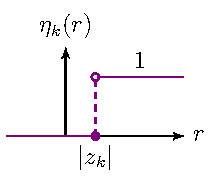
\includegraphics{Figuras/função salto.pdf} 
    \end{tabular}
    
    Então $n_f(r) = \dis{\sum_{k=1}^{N} \eta_k(r)}$. Segue que
    %
    \begin{align*}
        \sum_{k=1}^{N}\int_{|z_K|}^{R} \, \frac{dr}{r} 
        &= \sum_{k=1}^{N}\int_{|z_K|}^{R}\eta_k(r) \, \frac{dr}{r} \\
        &= \int_{|z_K|}^{R}\left(\sum_{k=1}^{N}\eta_k(r)\right) \, \frac{dr}{r} \\
        &= \int_{0}^{R}n_f(r) \, \frac{dr}{r}.
    \end{align*}
    %
    \end{proof}
    %
%\subsection{Ordem de crescimento e o número de zeros de uma função}
    % Agora, vamos usar a fórmula de Jensen para encontrar uma relação entre a
    % taxa de crescimento de uma função inteira no infinito e o comportamento
    % assintótico do número de zeros (contados com multiplicidade) desta
    % função dentro dos discos $D(0,R)$ quando $R\to +\infty$.
    
    % Primeiro, note que podemos reescrever a fórmula de Jensen da seguinte forma:
    % %
    % \begin{align*}
    %     \ln|f(0)| = \sum_{j=1}^n \ln\left|\frac{z_j}{R}\right| 
    %     + \frac{1}{2\pi}\int_0^{2\pi} \ln|f(Re^{i\theta})| \, d\theta,
    % \end{align*}
    % %
    % usando as propriedades do logaritmo e do valor absoluto.
    
    % Seja $f:U\subset\C\to\C$ é uma função holomorfa em $\overline{D(0,R)}$.
    % Para cada $r\in (0,R)$ denotamos por $n_f(r) \equiv n(r)$ o número de zeros 
    % de $f$, contados com multiplicidade, dentro do disco aberto $D(0,r)$.
    % Note que segue diretamente da definição que se $0 < r_1 \leq r_2 < R$, então
    % $n_f(r_1) \leq n_f(r_2)$, ou seja, $n_f$ é uma função não-decrescente. Usaremos
    % esse fato no seguinte lema que, por sua vez, será o primeiro de dois resultados
    % que nos permitirão extrair a relação entre zeros e a ordem de uma função.
    %
    % \begin{lema}
    % \label{lema:int-num-zeros}
    %     Sejam $R > 0$, $U\subseteq\C$ tal que $\overline{D(0,R)} \subseteq U$
    %     e $f:U\to\C$ uma função holomorfa. Se $z_1, z_2, \dots, z_n$ são zeros
    %     de $f$ em $D(0,R)$, então
    %     %
    %     \begin{equation*}
    %         \int_0^R n_f(r) \, \frac{dr}{r} 
    %         = \sum_{j=1}^n \ln\left|\frac{R}{z_j}\right|.
    %     \end{equation*}
    %     %
    % \end{lema}
    % %
    % \begin{proof}
    %     Note, primeiramente, que
    %     %
    %     \begin{equation*}
    %         \sum_{j=1}^n \ln\left|\frac{R}{z_j}\right| 
    %         = \sum_{j=1}^n \int_{|z_j|}^R \frac{1}{r} \, dr.
    %     \end{equation*}
    %     %
    %     Ademais, para cada $j=1, 2, \dots, n$, considere a função $\eta_j:\R\to\R$
    %     definida anteriormente:
    %     %
    %     \begin{equation*}
    %         \eta_j(r) 
    %         = \begin{cases}
    %         1, & |z_j| < r \\
    %         0, & |z_j| \geq r
    %         \end{cases}.
    %     \end{equation*}
    %     Daí, para cada $r$ fixado, temos
    %     %
    %     \begin{equation*}
    %         \sum_{j=1}^n \eta_j(r) = n_f(r),
    %     \end{equation*}
    %     %
    %     donde segue que
    %     %
    %     \begin{align*}
    %         \sum_{j=1}^n \int_{|z_j|}^R 1 \, \frac{dr}{r}
    %         = \sum_{j=1}^n \int_{0}^R \eta_j(r) \, \frac{dr}{r}
    %         = \int_{0}^R \left( \sum_{j=1}^n \eta_j(r) \right) \, \frac{dr}{r}
    %         = \int_{0}^R n_f(r) \, \frac{dr}{r},
    %     \end{align*}
    %     %
    %     como desejado.
    % \end{proof}
    %
    \noindent
    O segundo resultado que precisaremos é consequência imediata do 
    Corolário \ref{corol:num-zeros}.
    %
    \begin{corolario}
    \label{corol:jensen-com-zeros}
        Sejam $f:\C\to\C$ uma função inteira e $R>0$. Suponha que $f(0)\neq 0$
        e que $f(z)\neq 0$ para todo $z\in\partial D(0,R)$. Então
        %
        \begin{equation*}
            \int_0^R n_f(r) \, \frac{dr}{r}
            = \frac{1}{2\pi} \int_0^{2\pi} \ln|f(Re^{i\theta})| \, d\theta
            - \ln|f(0)|.
        \end{equation*}
        %
    \end{corolario}
    %
    \begin{proof}
       Pelo Corolário \ref{corol:num-zeros}, temos
       %
       \begin{equation*}
           \int_0^R n_f(r) \, \frac{dr}{r} 
           = \sum_{j=1}^n \ln\left|\frac{R}{z_j}\right|.
       \end{equation*}
       %
       Daí, basta usar esta identidade na fórmula de Jensen para obter o resultado.
    \end{proof}
    %
    \subsection{Funções de Ordem Finita de Crescimento}
    %
    \begin{definicao}[Ordem de Crescimento]
    \label{def:ordem-func}
    \index{Ordem de Crescimento}
        Seja $f:\C\to\C$ uma função inteira. Se existem um número positivo $\rho$
        e constantes $A,B>0$ tais que
        %
        \begin{equation*}
            |f(z)| \leq A\exp(B|z|^{\rho}),\quad  \forall z\in\C,
        \end{equation*}
        %
        dizemos que $f$ tem ordem de crescimento no máximo $\rho$. Definimos a
        ordem de crescimento de $f$ como sendo o número
        %
        \begin{equation*}
            \rho_f 
            \equiv 
            \inf 
            \left\{ 
                \rho > 0 :
                \begin{array}{c}
                    \exists m\ \textrm{constantes}\  
                    A\equiv A(\rho)>0\ \text{e}\ B\equiv B(\rho)>0 
                    \\[0.2cm]
                    \text{tais que}\ 
                    |f(z)| \leq A\exp(B|z|^{\rho}), \quad \forall z\in\C
                \end{array}
            \right\}.
        \end{equation*}
        %
    \end{definicao}
    %
    Alguns exemplos são:
    %
    \begin{itemize}
        \item a função $f:\C\to\C$ dada por $f(z) = e^z$ tem ordem de crescimento 1;
        \item a função $g:\C\to\C$ dada por $g(z) = e^{\alpha z^2 + z}, \alpha\in\C^*$
        tem ordem de crescimento 2;
        \item a função $f:\C\to\C$ dada por $f(z) = e^{e^z}$ não tem ordem de
        crescimento finita.
    \end{itemize}
    %
    \begin{teorema}
    \label{teo:est-num-zeros}
        Se $f:\C\to\C$ tem ordem de crescimento no máximo $\rho$, então:
        %
        \begin{enumerate}[(i)]
            \item $n_f(r) \leq Cr^{\rho}$ para algum $C>0$ e $r\gg 1$;
            \item se $z_1, z_2, \dots$ denotam os zeros de $f$, com $z_k\neq 0$,
            então para todo $s>\rho$ temos
            %
            \begin{equation*}
                \sum_{k=1}^{\infty} \frac{1}{|z_k|^s} < + \infty.
            \end{equation*}
            %
        \end{enumerate}
        %
    \end{teorema}
    %
    \begin{proof}
       Primeiro vamos mostrar que a conclusão do item {\it (i)} é válida. 
       Observe que basta mostrar que vale a estimativa
       %
       \begin{equation*}
           n_f(r) \leq Cr^{\rho}
       \end{equation*}
       %
       no caso em que $f$ não se anula na origem. 
       De fato, se $f(0) = 0$ e $k$
       é a multiplicidade de $0$, então a função $F:\C^*\to\C$ dada por 
       $F(z) = f(z)/z^k$ admite uma extensão inteira que não se anula na origem
       e além do mais $n_F(r) = n_f(r) - k$. Logo, para todo $r\geqslant 1$ temos
       %
       \begin{align*}
           n_f(r) = n_F(r) + k &\leq Cr^{\rho} + k \\
                               &\leq Cr^{\rho} + kr^{\rho} \\
                               &= (C+k) r^{\rho}.
       \end{align*}
       %

       
       Já que estamos assumindo que $f(0) \neq 0$, podemos aplicar o 
       Corolário \ref{corol:jensen-com-zeros}, que diz que
       %
       \begin{equation*}
           \int_0^R n_f(x) \, \frac{dx}{x} 
           = \frac{1}{2\pi} \int_0^{2\pi} \ln|f(Re^{i\theta})| \, d\theta - \ln|f(0)|.
       \end{equation*}
       %
       Escolhendo $R = 2r$ temos, pelas propriedades da integral, que
       %
       \begin{align*}
           \int_r^{2r} n_f(x) \, \frac{dx}{x}
           \leq \int_0^{2r} n_f(x) \, \frac{dx}{x}
           = \frac{1}{2\pi} \int_0^{2\pi} \ln|f(2re^{i\theta})| \, d\theta - \ln|f(0)|.
       \end{align*}
       %
       Lembrando que $n_f$ é monótona não-decrescente, temos a seguinte estimativa:
       %
       \begin{align*}
           \int_r^{2r} n_f(x) \, \frac{dx}{x}
           \geq n_f(r) \int_r^{2r} \frac{dx}{x} 
           = n_f(r)[\ln(2r) - \ln(r)]
           = n_f(r)\ln(2).
       \end{align*}
       %
       Por outro lado, segue da hipótese de $f$ 
       ter ordem de crescimento no máximo $\rho$ que
       %
       \begin{align*}
           \left| \frac{1}{2\pi} \int_0^{2\pi} \ln|f(2re^{i\theta})| \, d\theta \right|
           &\leq \frac{1}{2\pi} \int_0^{2\pi} \big|\ln|f(2re^{i\theta})| \big| \, d\theta 
           \\[0.2cm]
           &\leq \frac{1}{2\pi} \int_0^{2\pi} \ln\left(Ae^{B(2r)^{\rho}}\right) 
           \, d\theta 
           \\[0.2cm]
           &= \ln A + B2^{\rho}r^{\rho} 
           \\[0.2cm]
           &\leq r^{\rho}\ln A + B2^{\rho}r^{\rho} 
           \\[0.2cm]
           &= (\ln A + 2^{\rho}B)r^{\rho}.
       \end{align*}
       %
       Usando essas duas estimativas e tomando $r\gg 1$ (suficientemente grande),
       temos
       %
       \begin{align*}
           n_f(r)\ln(2) \leq \int_r^{2r} n_f(x) \, \frac{dx}{x} 
                        &\leq \int_0^{2r} n_f(x) \, \frac{dx}{x} 
                        \\[0.2cm]
                        &= \frac{1}{2\pi}\int_0^{2\pi} \ln|f(2re^{i\theta})| \, d\theta
                        - \ln|f(0)| 
                        \\[0.2cm]
                        &\leq (\ln A + 2^{\rho}B)r^{\rho} + \big|\ln|f(0)|\big| 
                        \\[0.2cm]
                        &\leq (\ln A + 2^{\rho}B)r^{\rho} + \big|\ln|f(0)|\big|r^{\rho} 
                        \\[0.2cm]
                        &= [\ln A + 2^{\rho}B + \big|\ln|f(0)|\big|]r^{\rho},
       \end{align*}
       %
       donde segue que
       %
       \begin{equation*}
           n_f(r) \leq \frac{\ln A + 2^{\rho}B + \big|\ln|f(0)|\big|}{\ln(2)}r^{\rho} 
           \equiv Cr^{\rho}.
       \end{equation*}
       %
       
       \medskip 
       Para provar a validade da conclusão do item {\it (ii)}, basta notar que
       %
       \begin{align*}
           \sum_{\substack{k\in\N \\ |z_k|\geq 1}} \frac{1}{|z_k|^s}
           &= \sum_{j=0}^{\infty} 
           \sum_{\substack{k\in\N \\ 2^j \leq |z_k| < 2^{j+1}}} \frac{1}{|z_k|^s} 
           \\[0.3cm]
           &\leq \sum_{j=0}^{\infty} \frac{1}{2^{sj}}n_f(2^{j+1})
           \\[0.2cm]
           &\leq \sum_{j=0}^{\infty} \frac{C}{2^{sj}}(2^{j+1})^{\rho} 
           \\[0.2cm]
           &\leq C2^{\rho} \sum_{j=0}^{\infty} 2^{(\rho - s)j}< +\infty,\quad 
           \text{se}\ \rho < s.
       \end{align*}
       %
    \end{proof}
    %
    
    Esse teorema merece alguns comentários. Primeiro, é importante observar que
    a demonstração do item {\it (ii)} se aproveita de uma certa 
    invariância na escala logarítmica da estimativa da integral
    de $n_{f}(x)/x$. Além disso, uma pergunta natural em relação ao item
    {\it (i)} seria: podemos fazer melhor, isto é, existe uma 
    estimativa mais forte para
    $n_f(r)$? A reposta é não, e o motivo fica claro nos seguintes exemplos.
    %
    \begin{exemplo}
        Considere a função $f:\C\to\C$ dada por $f(z) = \sen(\pi z)$, que tem
        zeros de ordem 1 nos inteiros. Ora, já que
        %
        \begin{align*}
            f(z) = \frac{e^{i\pi z} - e^{-i\pi z}}{2i},
        \end{align*}
        %
        temos que
        %
        \begin{align*}
            |f(z)| &\leq \frac{1}{2}\left( |e^{i\pi z}| + |e^{-i\pi z}| \right) \\
                   &\leq \frac{1}{2}\left( e^{\pi y} + e^{-\pi y} \right) \\
                   &\leq \frac{1}{2}\left( e^{\pi |z|} + e^{\pi |z|} \right) \\
                   &= e^{\pi |z|},
        \end{align*}
        %
        o que mostra que a ordem de crescimento de $f$ é no máximo 1. Por outro lado,
        tomando $z = ix$, podemos observar que
        %
        \begin{align*}
            |f(z)|=|f(ix)|&=\frac{1}{2}\left| e^{i\pi (ix)} - e^{-i\pi (ix)} \right| \\
                          &= \frac{1}{2}\left| e^{-\pi x} - e^{\pi x} \right| \\
                          &= \frac{1}{2} \left( e^{\pi x} - e^{-\pi x} \right) \\
                          &= \frac{1}{2}\left( 1 - e^{-2\pi x} \right)e^{\pi x} \\
                          &\geq \frac{1}{2}\left( 1 - e^{-2\pi} \right)e^{\pi x} \\
                          &= ce^{\pi |z|}.
        \end{align*}
        %
        Logo, $f$ tem ordem de crescimento $\rho = 1$. Daí, sendo
        %
        \begin{equation*}
            \mathcal{Z}(f) \equiv \{ z\in\C : f(z) = 0 \} = \mathbb{Z},
        \end{equation*}
        %
        temos, pelo teorema anterior,
        %
        \begin{align*}
            \sum_{k\in\mathbb{Z}^*} \frac{1}{|k|^s} 
            = \sum_{k=1}^{\infty} \frac{1}{|z_k|^s} < +\infty \text{ se } 1 = \rho < s.
        \end{align*}
        %
    \end{exemplo}
    %
    \begin{exemplo}
        Considere a função inteira $f:\C\to\C$ dada por
        %
        \begin{equation*}
            f(z) = \cos(z^{1/2}) \equiv \sum_{n=0}^{\infty} (-1)^n \frac{z^n}{(2n)!}.
        \end{equation*}
        %
        Note que não estamos falando da composta da função cosseno com o ramo
        principal da raiz quadrada, apesar da notação. Podemos pensar $f$ como
        continuação analítica dessa composta.
        
        Lembrando que
        %
        \begin{equation*}
            \cos z = \frac{e^{iz} + e^{-iz}}{2}
        \end{equation*}
        %
        e que $|e^z| \leq e^{|z|}$, temos
        %
        \begin{align*}
            |f(z)| &= \frac{1}{2}\left| 
            e^{i\exp\left(\frac{1}{2}(\ln|z| + i\arg z)\right)} 
            + e^{-i\exp\left(\frac{1}{2}(\ln|z| + i\arg z)\right)} \right| \\
            &= \frac{1}{2}\left| e^{i|z|^{1/2}\exp(i\arg z/2)} 
            + e^{-i|z|^{1/2}\exp(i\arg z/2)} \right| \\
            &\leq e^{ \left| i|z|^{1/2}\exp(i\arg z/2) \right| } \\
            &= e^{|z|^{1/2}}.
        \end{align*}
        %
        Portanto, a função $f$ tem crescimento no máximo $1/2$. 
        Observe que $f$ se anula 
        em $z_n = \dis \left( (n+1/2)\pi \right)^2$, para cada $n\in\mathbb{Z}$ e, ademais, a série
        %
        \begin{equation*}
            \sum_{n\in\mathbb{Z}} \frac{1}{|z_n|^s} < +\infty,
            \qquad \text{ sempre que } s > 1/2.
        \end{equation*}
        %
    \end{exemplo}
    %



    \bigskip 
    



    Uma outra pergunta interessante é: existe alguma função inteira cujos zeros são
    dados exatamente pela lista $z_1, z_2, \dots$, contados com multiplicidade? Dito
    de outro modo: dada uma lista de números complexos, conseguimos encontrar uma 
    função inteira cujos zeros são exatamente aqueles números?
    
    O ``candidato natural'', pensando em polinômios, seria
    %
    \begin{equation*}
        f(z) = \lim_{n\to\infty} (z-z_1)(z-z_2)\cdots(z - z_n).
    \end{equation*}
    %
    Mas refletindo um pouco sobre este limite, 
    rapidamente nos convenceríamos que esse produto 
    é complicado de se controlar, pois a cada novo valor de $n$ não
    só temos o dobro do número de parcelas que tínhamos anteriormente, como também todas estas parcelas se modificam a cada etapa.
    
    Weierstrass teve uma grande ideia para modificar 
    adequadamente a expressão acima de modo a
    obter um produto semelhante, mas que é sempre
    convergente (independentemente da escolha da lista $z_1,z_2,\ldots$) 
    e que se anula apenas em $z=z_j$, para cada $j\in\N$. 
    Trataremos disto na seção a seguir.
    
\section{Produtos Infinitos}
    \index{Produtos!infinitos}
    Dada uma sequência $\{ a_n \}_{n\in\N}$ de números complexos, dizemos que o
    produto $\dis{ \prod_{n=1}^{\infty} (1+a_n) }$ converge se existe o seguinte limite
    %
    \begin{equation}
    \index{Convergência!de produtos infinitos}
    \label{def-prod-infinito}
        \lim_{n\to\infty} \prod_{j=1}^n (1+a_j).
    \end{equation}
    %
    
    
    Embora fosse natural definir produtos infinitos de uma 
    dada sequência $\{ a_n \}_{n\in\N}$ de números complexos,
    diretamente pelo limite de seus produtos parciais, isto é, 
    $
    \lim_{n\to\infty} \prod_{j=1}^n a_j 
    \equiv 
    \lim_{n\to\infty}(a_1\cdot\ldots\cdot a_n)
    $, 
    seria muito mais difícil trabalhar com eles.
    Uma das dificuldades que resulta de tal definição é que o limite 
    de uma sequência da forma 
    $\prod_{j=1}^n a_j$
    pode convergir para zero sem que 
    nenhum dos fatores $a_j$'s seja nulo. 
    Por exemplo, considere a sequência $a_n\equiv 2^{-n}$, para todo 
    $n\in\mathbb{N}$. Neste caso, é fácil ver que 
    $
    \lim_{n\to\infty}\prod_{j=1}^n a_j
    =
    \lim_{n\to\infty}\prod_{j=1}^n 2^{-j} 
    = 
    \lim_{n\to\infty}2^{-(n^2+n)/2}
    =
    0
    $
    e evidentemente nenhum dos $a_n$'s é nulo.
    
    Definimos a noção de produto infinito 
    como feito em \eqref{def-prod-infinito} para podermos garantir
    que um produto infinito é nulo se, e somente se,
    um de seus fatores é nulo. 
    Provamos este fato na proposição abaixo.
    Esta propriedade é fundamental nas provas dos 
    resultados mais importante desta
    seção que são os Teoremas de fatoração de Weierstrass e Hadamard. 
    Além do mais, adotando esta definição 
    conseguimos um critério simples para a convergência destes
    produtos infinitos, em termos de séries infinitas, objetos que 
    sabemos manipular muito bem.
    
    
    %
    \begin{proposicao}
    \label{prop:prod-inf}
        Se $\dis{\sum_{n\in\N} |a_n| < +\infty }$, então o produto
        $\dis{ \prod_{n=1}^{\infty} (1+a_n) }$ converge. Ademais, o produto converge
        para zero se, e somente se, um de seus fatores é nulo, ou seja, existe
        $k\in\N$ tal que $1+a_k = 0$.
        Por último, a ordem dos fatores no produtório é irrelevante, ou seja, 
        %
        \[
        \prod_{n=1}^{\infty} (1+a_n) = \prod_{n=1}^{\infty} (1+a_{\tau(n)})
        \]
        %
        para qualquer permutação $\tau$ de $\N$.
    \end{proposicao}
    %
    \begin{proof}
       Se $\dis{\sum_{n\in\N} |a_n| < +\infty }$, então existe $n_0\in\N$
       tal que se $n\geq n_0$ então $|a_n| < 1/2$. Para simplificar o 
       argumento, vamos supor que esta desigualdade é válida para todo $n\in\N$.
       
       Considere o ramo principal do logaritmo e a sequência $\log(1+a_n)$.
       É claro que se $|z| < 1/2$, então
       %
       \begin{equation*}
           1 + z = e^{\log(1+z)}.
       \end{equation*}
       %
       Portanto, os produtos parciais podem ser escritos como
       %
       \begin{equation*}
           \prod_{j=1}^n (1 + a_j) = \prod_{j=1}^n e^{\log(1 + a_j)} = e^{B_n},
       \end{equation*}
       %
       sendo
       %
       \begin{equation*}
           B_n = \sum_{j=1}^n \underbrace{\log(1 + a_j)}_{b_j}.
       \end{equation*}
       %
       Usando expansão em série de potências, temos que
       %
       \begin{align*}
           |\log(1+w)|&=\left| \sum_{n=0}^{\infty} (-1)^n \frac{w^{n+1}}{n+1} \right| \\
                      &\leq |w|\cdot\left| 1 - \frac{w}{2} + \frac{w^2}{3} 
                      - \cdots \right| \\
                      &\leq |w|\cdot\frac{1}{1 - |w|} \\
                      &\leq 2|w|,
       \end{align*}
       %
       considerando $|w| \leq 1/2$. Portanto,
       %
       \begin{equation*}
           |B_n| = \left| \sum_{j=1}^n \log(1 + a_j) \right| 
           \leq \sum_{j=1}^n |\log(1+a_j)|
           \leq \sum_{j=1}^n 2|a_j|,
       \end{equation*}
       %
       ou seja, $B_{\infty}$ é absolutamente convergente, isto é, existe
       $B\in\C$ tal que $B_n \xrightarrow{n\to\infty} B$. Ora, já que
       %
       \begin{equation*}
           \prod_{j=1}^n (1+a_j) = e^{B_n},
       \end{equation*}
       %
       segue que existe
       %
       \begin{equation*}
           \lim_{n\to\infty} \prod_{j=1}^n (1+a_j) = \lim_{n\to\infty} e^{B_n} = e^B.
       \end{equation*}
       %
       Além disso, observe que se $1+a_n \neq 0$ para todo $n\in \N$, então
       %
       \begin{equation*}
           \left| \prod_{j=1}^{\infty} (1+a_j) \right| = |e^B| \neq 0.
       \end{equation*}
       %
       Por último, note que se $\tau$ for uma permutação em $\N$ e 
       trocarmos $a_j$ por $a_{\tau(j)}$ nas expressões
       envolvendo os $B_n$'s, chegaremos à conclusão de que, ainda assim,
       $B_n\xrightarrow{n\to\infty} B$. Portanto, a convergência do produtório de Weierstrass
       é invariante por permutação dos fatores.
    \end{proof}
    %
    
    O próximo passo é falar de produtos infinitos de funções holomorfas.
    %
    \begin{proposicao}
    \label{prop:prod-inf-func-holom}
        Seja $\{ F_n \}_{n\in\N}$ uma sequência de funções holomorfas
        definidas em um domínio $\Omega\subseteq\C$. Se existem constantes
        $c_n>0$ tais que 
        \[ 
        \sum_{n\in\N} c_n < +\infty 
        \quad\text{e}\quad 
        \sup_{z\in\Omega} |F_n(z) - 1| \leq c_n, \, \forall n\in\N,
        \]
        então:
        %
        \begin{enumerate}[(i)]
            \item o produto infinito $\dis{ \prod_{n=1}^{\infty} F_n(z) }$ converge
            uniformemente em $\Omega$ para uma função holomorfa $F(z)$;
            \item se para cada $n\in\mathbb{N}$ temos que $F_n(z) \neq 0$, para todo  
            $z\in\Omega$, então 
            \[
            \frac{F'(z)}{F(z)} = \sum_{n=1}^{\infty} \frac{F_n'(z)}{F_n(z)}.
            \]
        \end{enumerate}
        %
    \end{proposicao}
    %
    \begin{proof}
       Vamos começar com (i). Note que para cada $z\in\Omega$ fixado podemos
       escrever $F_n(z) = 1 + a_n(z)$. Ademais, segue da hipótese que
       $|a_n(z)| = |F_n(z) - 1| \leq c_n$ e que
       %
       \begin{equation*}
           \sum_{n\in\N} |a_n(z)| \leq \sum_{n\in\N} c_n < +\infty.
       \end{equation*}
       %
       Logo, existe
       %
       \begin{equation*}
           \lim_{n\to\infty} \prod_{j=1}^n F_j(z) 
           = \lim_{n\to\infty} \prod_{j=1}^n [1 + a_j(z)].
       \end{equation*}
       %
       Além disso, os produtos parciais de $F_j$ convergem uniformemente, uma vez
       que sendo $D' = \dis{ D\left( 0, 2\sum_{n\in\N} c_n \right) }$, temos
       %
       \begin{align*}
           \left| \prod_{j=1}^{m+n} F_j(z) - \prod_{j=1}^{n} F_j(z) \right|
           &=\left|\prod_{j=1}^{m+n} [1+a_j(z)] - \prod_{j=1}^{n} [1+a_j(z)] \right| \\
           &= \left| e^{B_{m+n}(z)} - e^{B_n(z)} \right| \\
           &= \left| \int_{B_n(z)}^{B_{m+n}(z)} e^w \, dw \right| \\
           &\leq \sup_{w\in D'} 
           |e^w|\cdot |B_{m+n}(z) - B_n(z)| \\
           &= k|B_{m+n} - B_n(z)| \xrightarrow{m,n\to\infty} 0.
       \end{align*}
       %
       Logo, a função
       %
       \begin{equation*}
           z \mapsto \lim_{n\to\infty} \prod_{j=1}^n F_j(z) 
                                       \equiv \prod_{j=1}^{\infty} F_j(z)
                                       \equiv F(z)
       \end{equation*}
       %
       é holomorfa em $\Omega$.
       
       Agora, para o item (ii), seja $K\subseteq\Omega$ um subconjunto compacto
       e defina
       %
       \begin{equation*}
           G_n(z) = \prod_{j=1}^n F_j(z), \forall z\in\Omega.
       \end{equation*}
       %
       Já que $G_n \xrightarrow[\text{unif}]{n\to\infty} F$, temos que
       $G_n' \xrightarrow[\text{unif em compactos}]{n\to\infty} F'$.
       Para ver isto basta observar que
       %
       \begin{equation*}
           G_n'(z) - F'(z) = 
           \frac{1}{2\pi i} \int_{\y} (G_n(w) - F(w))\frac{1}{(w-z)^2} \, dw
       \end{equation*}
       %
       sendo $\y$ como ilustrado abaixo.
       %
       \begin{figure}[H]\centering
           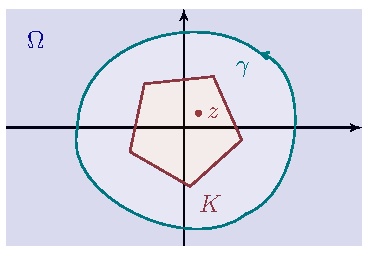
\includegraphics{Figuras/y para Gn'-Fn'.pdf}
       \end{figure}
       %
       Por hipótese, $F_n(z) \neq 0$ para todos $n\in\N$ e $z\in\Omega$, de modo
       que $F(z)\neq 0$ para todo $z\in\Omega$. Já que $F$ é holomorfa e, 
       consequentemente, contínua, podemos dizer que
       %
       \begin{equation*}
           \inf_{z\in K} |F(z)| = F(z_*) > 0.
       \end{equation*}
       %
       Portanto, podemos garantir que $G_n(z)$ é uniformemente limitada inferiormente
       em $n$ e $z\in K$. De fato,
       %
       \begin{align*}
           \inf_{z\in K} |G_n(z)| = \inf_{z\in K} |G_n(z) - F(z) + F(z)|
           \geq \inf_{z\in K} | |G_n(z) - F(z)| - |F(z)| |.
       \end{align*}
       %
       Como $G_n$ converge uniformemente para $F$, existe $n_0\in\N$ tal que
       se $n\geq n_0$, então 
       $|G_n(z) - F(z)| < \dis{\frac{1}{2} F(z_*) }$ para todo 
       $z\in K$. Logo, para todo $n\geq n_0$ temos
       %
       \begin{equation*}
           \inf_{z\in K} |G_n(z)| > \frac{1}{2}\inf_{z\in K} |F(z)| 
                                  = \frac{1}{2} F(z_*) > 0.
       \end{equation*}
       %
       Por outro lado, se $n\leq n_0$, então como $F_j(z)\neq 0$ para todo 
       $z\in\Omega$, temos que
       %
       \begin{align*}
           \inf_{z\in K} |G_n(z)| &= \inf_{z\in K} |F_1(z)|\cdots|F_n(z)| \\
                                  &\geq \prod_{j=1}^n \inf_{z\in K} |F_j(z)| \\
                                  &= |F_1(z^1_*)| \cdots |F_n(z^n_*)| \equiv I_K.
       \end{align*}
       %
       Portanto, 
       %
       \begin{equation*}
           \inf_{n\in\N} \inf_{z\in K} |G_n(z)| 
           \geq \min\left\{ I_K, \frac{1}{2}|F(z_*)| \right\} > 0,
       \end{equation*}
       %
       donde segue que 
       %
       \begin{equation*}
           \frac{G_n'}{G_n} \xrightarrow[\text{unif. em } K]{n\to\infty} \frac{F'}{F}
       \end{equation*}
       %
       para cada $z\in K$ e, como $K$ é compacto arbitrário, segue que
       %
       \begin{equation*}
           \frac{G_n'(z)}{G_n(z)} \xrightarrow{n\to\infty} \frac{F'(z)}{F(z)}
       \end{equation*}
       %
       para cada $z\in\Omega$. Observe que não podemos garantir que essa última
       convergência é uniforme em $\Omega$.
       
       Ademais, para cada $n\in\N$ temos
       %
       \begin{align*}
           \frac{G_n'(z)}{G_n(z)} 
           &= \frac{ \frac{d}{dz}[F_1(z)\cdots F_n(z)] }{F_1(z)\cdots F_n(z)} \\
           &= \sum_{j=1}^n F'_j(z)
           \frac{F_1(z)\cdots F_{j-1}(z)F_{j+1}(z)\cdots F_n(z)}{F_1(z)\cdots F_n(z)} 
           \\
           &= \sum_{j=1}^n \frac{F'_j(z)}{F_j(z)},
       \end{align*}
       %
       o que mostra que
       %
       \begin{equation*}
           \frac{F'(z)}{F(z)} = \lim_{n\to\infty} \frac{G'_n(z)}{G_n(z)}
                              = \lim_{n\to\infty} \sum_{j=1}^n \frac{F'_j(z)}{F_j(z)}
                              \equiv \sum_{j=1}^{\infty} \frac{F'_j(z)}{F_j(z)}.
       \end{equation*}
       %
    \end{proof}
    %
    
    Vamos usar este teorema para trabalhar com um exemplo interessante.
    \begin{exemplo}[A fórmula do produto da função seno]
    \index{Fórmula! do produto da função seno}
        Vamos estabelecer a validade da seguinte fórmula:
        %
        \begin{equation*}
            \frac{\sen(\pi z)}{\pi} = z\prod_{n=1}^{\infty} 
            \left( 1 - \frac{z^2}{n} \right).
        \end{equation*}
        %
        Para tanto, vamos estabelecer uma fórmula para $\cot(\pi z)$.
        Apesar de parecer estranha, a escolha da função cotangente é tudo menos
        coincidência. De fato, devido à Proposição \ref{prop:prod-inf-func-holom},
        para encontrar uma fórmula do produto da função $\sen(\pi z)/\pi$ precisaremos 
        considerar a sua derivada logarítmica, que nada mais é que $\pi\cot(\pi z)$.
        
        Vamos então mostrar que, para todo $z\in\C\setminus\mathbb{Z}$, temos
        %
        \begin{equation*}
            \pi\cot(\pi z) = \sum_{n=-\infty}^{\infty} \frac{1}{z+n}
                           \equiv \lim_{n\to\infty} \sum_{|j|\leq n} \frac{1}{z+j}
                           = \frac{1}{z} + \sum_{n=1}^{\infty} \frac{2z}{z^2 - n^2},
        \end{equation*}
        %
        onde usamos que
        %
        \begin{equation*}
            \frac{1}{z+n} + \frac{1}{z-n} = \frac{2z}{z^2 - n^2}.
        \end{equation*}
        %
        A estratégia para mostrar essa identidade será mostrar que tanto
        $F(z) = \pi\cot(\pi z)$ e $S(z) = \dis{\frac{1}{z} + 
        \sum_{n=1}^{\infty} \frac{2z}{z^2- n^2}}$ satisfazem as seguintes propriedades:
        %
        \begin{enumerate}[(i)]
            \item $H(z+1) = H(z)$;
            \item $H(z) = \dis{ \frac{1}{z} + H_0(z) }$, sendo $H_0$ analítica próxima
            do zero;
            \item $H(z)$ tem polos simples em $\Z$ e nenhuma outra singularidade.
        \end{enumerate}
        %
        De fato, para $F$,
        %
        \begin{enumerate}[(i)]
            \item 
            %
            \begin{align*}
                F(z+1)=\pi\cot(\pi(z+1)) &= \pi\frac{\cos(\pi(z+1))}{\sen(\pi(z+1))} \\
                                         &= \pi\frac{-\cos(\pi z)}{-\sen(\pi z)} \\
                                         &= \pi\cot(\pi z) \\
                                         &= F(z).
            \end{align*}
            %
            \item 
            %
            \begin{align*}
                \lim_{z\to 0} zF(z) &= \lim_{z\to 0} \pi z 
                \frac{\cos(\pi z)}{\sen(\pi z)} \\
                &= \lim_{z\to 0} \cos(\pi z)\cdot\frac{\pi z}{\sen(\pi z)} \\
                &= \lim_{z\to 0} \frac{\pi z}{\sen(\pi z)} \\
                &= 1 = \res(F,0).
            \end{align*}
            %
            Como $F$ tem apenas singularidades isoladas em $\Z$, segue do
            teorema de Laurent que para todo $z\in A(0,0,1)$ temos
            %
            \begin{equation*}
                F(z) = \frac{\res(F,0)}{z} + H_0(z) = \frac{1}{z} + H_0(z),
            \end{equation*}
            %
            com $H_0$ holomorfa em $D(0,1).$
            
            \item $F$ é claramente holomorfa em $\C\setminus\Z$.
        \end{enumerate}
        %
        Agora, para $S$, temos
        %
        \begin{enumerate}[(i)]
            \item $\forall z\in\C\setminus\Z$:
            %
            \begin{align*}
                S(z+1) &= \lim_{n\to\infty} \sum_{|j|\leq n} \frac{1}{z+1+j} \\
                       &= \lim_{n\to\infty}\left( \sum_{|j|\leq n+1} \frac{1}{z+j}
                       - \frac{1}{z-n-1} - \frac{1}{z-n} \right) \\
                       &= \lim_{n\to\infty} \sum_{|j|\leq n} \frac{1}{z_j} \\
                       &= S(z)
            \end{align*}
            %
            \item $\forall z\in D(0,1/2)$, temos
            %
            \begin{equation*}
                S(z) = \frac{1}{z} + \sum_{n=1}^{\infty} \frac{2z}{z^2 - n^2}.
            \end{equation*}
            %
            Considere a sequência de funções $h_n:D(0,1/2)\to\C$ dada por
            $h_n(z) = \dis{ \frac{2z}{z^2 - n^2} }$. Para cada $n\in\N$, temos
            que $h_n$ é uma função holomorfa e, além disso,
            %
            \begin{align*}
                \sup_{z\in D(0,1/2)} |h_n(z)| 
                = \sup_{z\in D(0,1/2)} \left| \frac{2z}{n^2
                \left( \frac{z^2}{n^2} - 1 \right)} \right|
                = \frac{2}{n^2}\sup_{z\in D(0,1/2)} 
                \frac{|z|}{\left| \frac{z^2}{n^2} - 1 \right|}
                = \frac{2}{n^2}.
            \end{align*}
            %
            Logo,
            %
            \begin{equation*}
                \sum_{n=1}^{\infty} \sup_{z\in D(0,1/2)} |h_n(z)|
                \leq 2\sum_{n=1}^{\infty} \frac{1}{n^2} < +\infty.
            \end{equation*}
            %
            Pelo teste M de Weierstrass, segue que 
            $\dis{ \sum_{n=1}^{\infty} h_n(z) \equiv S_0(z) }$ define uma função
            $S_0: D(0,1/2) \to\C$ holomorfa. Assim, 
            %
            \begin{equation*}
                S(z) = \frac{1}{z} + S_0(z),
            \end{equation*}
            %
            com $S_0$ holomorfa em $D(0,1/2)$.
            
            \item Fixado $n\in\Z$, temos que
            %
            \begin{align*}
                S(z) &= \frac{1}{z} + \sum_{j\in\N\setminus\{n\}} \frac{2z}{z^2 - j^2}
                + \frac{2z}{z^2 - n^2} \\
                &= S_1(z) + \frac{1}{z+n} + \frac{1}{z-n}.
            \end{align*}
            %
            Pelo teste M de Weierstrass, segue que $S_1(z) + \dis{\frac{1}{z+n}}$
            é holomorfa em $D(n, 1/2)$, de modo que $S$ tem apenas polos simples
            em cada ponto de $\Z$.
        \end{enumerate}
        %
        Sabendo que $F$ e $S$ satisfazem (i), (ii) e (iii), podemos afirmar que
        $H:\C\setminus\Z\to\C$ dada por
        %
        \begin{equation*}
            H(z) \equiv F(z) - S(z)
        \end{equation*}
        %
        satisfaz $H(z+1) = H(z)$. Ademais, segue da propriedade (ii) que
        $\res(H,0) = 0$, de modo que $z=0$ é uma singularidade removível de $H$.
        Esta informação, junto com a periodicidade de $H$ dada pelo item (i)
        implica que, para todo $n\in\Z$,
        %
        \begin{equation*}
            \lim_{z\to n} H(z) = \lim_{z\to n} H(z-n) = \lim_{z\to 0} H(z) = 0.
        \end{equation*}
        %
        Logo, segue do teorema de Riemann que $H$ admite extensão inteira.
        
        Para estabelecer a fórmula da cotangente, é suficiente mostrar que
        $H$ é limitada e usar o teorema de Liouville.
        
        Ademais, para mostrar que $H$ é limitada, basta trabalhar na faixa
        %
        \begin{equation*}
            S_{\frac{1}{2}} = \left\{ z\in\C : |\Re(z)| \leq \frac{1}{2} \right\},
        \end{equation*}
        %
        uma vez que $H$ satisfaz a periodicidade (i).
        %
        \begin{figure}[H]\centering
            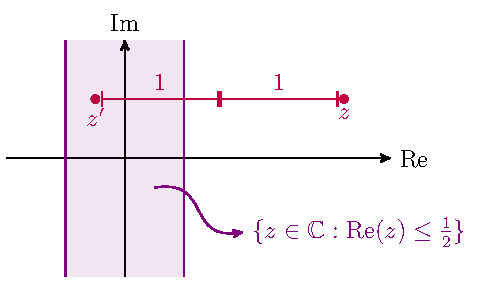
\includegraphics{Figuras/S_meio.pdf}
        \end{figure}
        %
        Já que $H:\C\to\C$ é inteira, então $H$ é limitada em
        %
        \begin{equation*}
            \Omega_1 = S_1 \cap S_{\frac{1}{2}},
        \end{equation*}
        %
        com
        %
        \begin{equation*}
            S_1 = \{ z\in\C : |\Im(z)| \leq 1 \},
        \end{equation*}
        %
        ou seja, 
        %
        \begin{equation}
            \sup_{z\in \Omega_1} |H(z)| = k_1 < +\infty
        \end{equation}
        %
        pois $\Omega_1$ é um compacto, como ilustrado abaixo.
        %
        \begin{figure}[H]\centering
            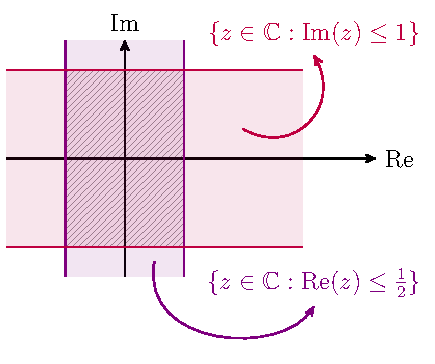
\includegraphics{Figuras/S_meio cap S_1.pdf}
            \caption{%
                A região hachurada, $\Omega_1$, é um compacto.
            }
        \end{figure}
        %
        Para terminar a demonstração que $H$ é limitada em $S_{\frac{1}{2}}$,
        resta analisar o que acontece com a função em
        %
        \begin{equation*}
            \Omega_2 = S_{\frac{1}{2}} \cap \left\{ z\in\C : |\Im(z)| > 1 \right\}.
        \end{equation*}
        %
        Ora, se $z = x + iy$, então
        %
        \begin{align*}
            \cot(\pi z) &= 
            i\frac{ e^{i\pi z} + e^{-i\pi z} }{ e^{i\pi z} - e^{-i\pi z} } \\
            &= i\frac{ e^{i\pi x}e^{-\pi y} + e^{-i\pi x}e^{\pi y} }
            { e^{i\pi x}e^{-\pi y} - e^{-i\pi x}e^{\pi y} } \\
            &= i\frac{ e^{-2\pi y} + e^{-2\pi ix} }{ e^{-2\pi y} - e^{-2\pi ix} }.
        \end{align*}
        %
        Como estamos supondo $|y|>1$, segue que
        %
        \begin{align*}
            |\cot(\pi z)| = 
            \left| 
            \frac{ e^{-2\pi y} + e^{-2\pi ix} }{ e^{-2\pi y} - e^{-2\pi ix} } 
            \right|
            \leq \frac{ 1 + e^{-2\pi y} }{ 1 - e^{-2\pi y} }
            \leq \widetilde{k_1}.
        \end{align*}
        %
        Ainda para $|y|>1$ e $|x|\leq 1/2$, temos
        %
        \begin{align*}
            \left| 
            \frac{1}{z} + \sum_{n=1}^{\infty} \frac{2z}{z^2 - n^2} 
            \right|
            &= \left| 
            \frac{1}{x+iy} + \sum_{n=1}^{\infty} \frac{2(x+iy)}{x^2 - y^2 - n^2 +2ixy} 
            \right| \\
            &\leq \frac{1}{\sqrt{x^2 + y^2}} 
            + \sum_{n=1}^{\infty} \frac{|2x|}{\sqrt{(x^2 - y^2 - n^2)^2 + 4x^2y^2}} \\
            &+ \sum_{n=1}^{\infty} \frac{|2y|}{\sqrt{(x^2 - y^2 - n^2)^2 + 4x^2y^2}} \\
            &\leq 1 
            + \sum_{n=1}^{\infty} \frac{1}{|y|^2 + n^2 - 1/4}
            + \sum_{n=1}^{\infty} \frac{|2y|}{|y|^2 + n^2 - 1/4} \\
            &\leq 1 + \sum_{n=1}^{\infty} \frac{1}{n^2} 
            + 2\sum_{n=1}^{\infty} \frac{|y|}{|y|^2/4 + n^2 - n^2/4} \\
            &\leq 1 + \frac{\pi^2}{6} + 
            8\sum_{n=1}^{\infty} \frac{|y|}{\frac{1}{4}(|y|^2 + 3n^2)} \\
            &\leq 1 + \frac{\pi^2}{6} +
            8\sum_{n=1}^{\infty} \frac{|y|}{|y|^2 + n^2}.
        \end{align*}
        %
        Agora, como $b:(0, +\infty)\to\R$ dada por $\dis{ b(x) = \frac{|y|}{|y|^2 + x^2} }$
        é decrescente já que
        %
        \begin{equation*}
            b'(x) = |y|\frac{-2x}{(|y|^2 + x^2)^2} < 0 \, \forall x+iy \in\Omega_2,
        \end{equation*}
        %
        podemos assegurar que
        %
        \begin{equation*}
            \sum_{n=1}^{\infty} \frac{|y|}{|y|^2 + n^2} 
            \leq
            \int_0^{\infty} \frac{|y|}{|y|^2 + x^2} \, dx.
        \end{equation*}
        %
        \begin{figure}[H]\centering
            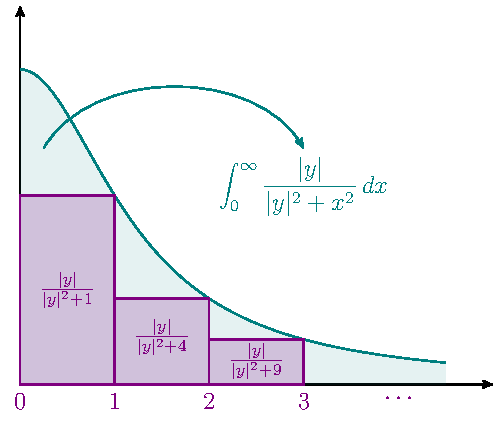
\includegraphics{%
                Figuras/majoração por integral.pdf
            }
        \end{figure}
        %
        Agora, considerando a mudança de variáveis $u = x/|y|$, temos
        %
        \begin{align*}
            \int_0^{\infty} \frac{|y|}{|y|^2 + x^2} \, dx = 
            \int_0^{\infty} \frac{1}{1 + u^2} \, du =
            \frac{\pi}{2}.
        \end{align*}
        %
        Até o momento, mostramos que
        %
        \begin{enumerate}
            \item $|\cot(\pi z)| = \dis{ 
            \left|\frac{ e^{-2\pi y} + e^{-2i\pi x} }{ e^{-2\pi y} - e^{-2i\pi x} } \right|
            \leq \frac{ 1 + e^{-2\pi y} }{ 1 - e^{-2\pi y} }
            \leq \widetilde{k_1}}$;
            
            \item $|S(z)| = \dis{ 
            \left| \frac{1}{z} + \sum_{n=1}^{\infty} \frac{2z}{z^2 - n^2} \right| 
            \leq 1 + \frac{\pi^2}{6} + 8\int_0^{\infty} \frac{|y|}{|y|^2 + x^2} \, dx
            = 1 + \frac{\pi^2}{6} + 4\pi =
            \widetilde{k_2}}$,
        \end{enumerate}
        %
        donde segue que
        %
        \begin{align*}
            \sup_{z\in\Omega_2} |H(z)| \leq 
            \sup_{z\in\Omega_2} |F(z) - S(z)| \leq
            \pi\widetilde{k_1} + \widetilde{k_2} \equiv
            k.
        \end{align*}
        %
        Portanto, lembrando que $H$ é periódica, temos
        %
        \begin{equation*}
            \sup_{z\in\C} |H(z)| =
            \sup_{z\in\Omega_1\cup\Omega_2} |H(z)| \leq
            k,
        \end{equation*}
        %
        ou seja, $H$ é limitada em $\C$.
        Pelo teorema de Liouville, como $H$ é inteira, temos
        $H(z)$ constante. 
        Agora, note que $H$ pode ser vista como extensão holomorfa de $F(z) - S(z)$,
        que é uma função ímpar. Portanto, $H$ 
        também é ímpar e $H(0) = 0$, donde segue 
        que $H\equiv 0$, ou seja, $F(z) \equiv S(z)$ e temos
        %
        \begin{equation*}
            \pi\cot(\pi z) = \frac{1}{z} + \sum_{n=1}^{\infty} \frac{2z}{z^2 - n^2},
            \, \forall z\in\C\setminus\Z.
        \end{equation*}
        %
        Finalmente, para mostrar a fórmula de produto para o seno, sejam
        %
        \begin{align*}
            G(z) &= \frac{\sen(\pi z)}{\pi} , \\
            P(z) &= z\prod_{n=1}^{\infty} \left( 1 - \frac{z^2}{n^2} \right).
        \end{align*}
        %
        Para mostrar a convergência de $P(z)$, vamos usar a 
        Proposição \ref{prop:prod-inf-func-holom} com $P(z) = zF(z)$, 
        $\Omega = D(0,R)\setminus\Z$,
        $F_n(z) = 1 - \dis{ \frac{z^2}{n^2} }$. Daí, temos
        %
        \begin{equation*}
            |F_n(z) - 1| \leq \sup_{z\in\Omega} \frac{|z|^2}{n^2} = \frac{R^2}{n^2}
            \equiv c_n.
        \end{equation*}
        %
        Portanto, para todo $z\in\Omega$,
        %
        \begin{align*}
            \frac{P'(z)}{P(z)} =
            \frac{1}{z} + \sum_{n=1}^{\infty} \frac{ -\frac{2z}{n^2} }{ 1 - \frac{z^2}{n^2} }
            = \frac{1}{z} + \sum_{n=1}^{\infty} \frac{2z}{z^2 - n^2}.
        \end{align*}
        %
        Agora, como $G'(z)/G(z) = \pi\cot(\pi z)$, 
        o resultado que acabamos de mostrar
        nos dá, para todo $z\in\Omega$,
        %
        \begin{equation*}
            \left( \frac{P(z)}{G(z)} \right)'
            = \frac{ P'(z)G(z) - P(z)G'(z) }{ G^2(z) }
            = \frac{P(z)}{G(z)}\left[ \frac{P'(z)}{P(z)} - \frac{G'(z)}{G(z)} \right]
            \equiv 0,
        \end{equation*}
        %
        de modo que $P(z) = cG(z)$ para alguma constante $c, \, \forall z\in\Omega$,
        pois $\Omega$ é conexo. 
        Ora, então
        %
        \begin{equation*}
            1 
            = \lim_{z\to 0} \prod_{n=1}^{\infty} \left( 1 - \frac{z^2}{n^2} \right)
            = \lim_{z\to 0} \frac{P(z)}{z} 
            = c\lim_{z\to 0} \frac{G(z)}{z}
            = c\lim_{z\to 0} \frac{\sen(\pi z)}{\pi z}
            = c,
        \end{equation*}
        %
        onde usamos que o produtório é holomorfo.
        Portanto, $P(z) = G(z)$ para todo $z\in\Omega$. 
        Pelo Princípio da Identidade,
        como $\Omega$ é aberto e conexo, segue que essa identidade vale para todo
        $z\in\C$.
    \end{exemplo}
    %
    \begin{exercicio}
        Use a série de Taylor de $\sin z$ e a identidade 
        % 
        \[
          \sin \pi z = \pi z\prod_{n=1}^\infty \left(1 - \frac{z^2}{n^2}\right),
        \]
        %
        deduzida acima, para demonstrar que 
        %
        \[
          \sum_{n=1}^\infty \frac{1}{n^2} = \frac{\pi^2}{6}.
        \]
    \end{exercicio}
    %
    
\section{O Teorema de Weierstrass}
    
    Anteriormente, vimos que, para construir uma função com zeros prescritos 
    na forma de uma lista ou sequência $\{a_n\}$, 
    uma tentativa ingênua era escrever
    %
    $$ f(z) = \lim_{n \to \infty} (z-a_1) \cdots (z-a_n).$$
    %
    Produtos como esse (em geral) não convergem para qualquer sequência 
    escolhida $\{a_n\}$, então essa não é a melhor escolha para construir $f$. 
    
    Mostramos, também, que vale a igualdade 
    %
    $$\frac{\sin{\pi z}}{\pi} = z \prod_{n = 1}^{\infty} \left(1 - \frac{z^2}{n^2}\right)$$
    %
    e a função $\sin{\pi z}$ se anula exatamente em $\mathbb{Z}$. 
    Analisando o produto com mais cuidado, vemos que cada fator é da forma 
    $(n^2 - z^2)/n^2 = (n - z)(n + z)/n^2$ 
    que se anula exatamente em $\pm n \in \Z$. 
    Além disso, o fato de termos escolhido fatores 
    %
    $$\left(1 - \frac{z^2}{n^2}\right)$$
    %
    em vez de $(n^2 - z^2)$ 
    nos permitiu usar a Proposição \ref{prop:prod-inf-func-holom}. 
    
    Se queremos definir uma função que se anula precisamente em uma sequência 
    qualquer $\{a_n\}$ de uma forma análoga à vista acima, ter $z^2$ nos 
    fatores pode não ser vantajoso, pois $-a_n$ pode não estar na sequência e mesmo 
    assim anular a função se $a_n$ anulá-la. Ademais, o fator $z^2$ não teve nenhuma 
    importância particular em termos de estimativas a nosso favor. Portanto, um bom 
    caminho é considerar fatores da forma
    %
    $$ \left(1 - \frac{z}{a_n}\right)g_n(z), $$
    %
    onde $g_n(z)$ são funções que facilitariam a convergência. O grande problema 
    está em como escolher tais funções e é neste ponto que reside a maior 
    contribuição de Weierstrass: ele encontrou funções que garantem a 
    convergência dada qualquer sequência $\{a_n\}$.
    
    Vamos enunciar o grande resultado desta seção agora 
    e demonstrá-lo no decorrer do texto.
    
    \begin{teorema}[Teorema do Produto de Weierstrass]
    \label{teo-Weierstrass-fatoracao}
    \index{Teorema!do Produto de Weierstrass}
        Dada uma sequência $\{a_n\}$ de números complexos tal que 
        $|a_n| \to \infty$, quando $n \to \infty$, 
        existe uma função inteira $f: \C \to \C$ que 
        se anula em $z=a_n$, para cada $n\in\mathbb{N}$, 
        e não se anula em quaisquer outros pontos do plano complexo.
        
        Além do mais, se $a_m\neq a_n$ 
        para todo $m\neq n$, então, para 
        cada $n\in\N$ temos que $z=a_n$ 
        é um zero simples de $f$ (multiplicidade um). 
    \end{teorema}
 
 \bigskip 
    
    Note que não é possível existir uma função como no enunciado do Teorema
    de Weierstrass, quando a sequência $\{a_n\}$ 
    assume infinitos valores distintos e
    a condição $|a_n| \xrightarrow{n\to\infty} \infty$ não é satisfeita.
    De fato, suponha por absurdo que exista tal função. 
    Já que $\{a_n\}$ toma infinitos valores distintos e 
    a sequência $|a_n|$ não tende a infinto, quando $n\to \infty$,
    podemos encontrar algum $R>0$ e infinitos elementos distintos 
    da sequência $\{a_n\}$ dentro do disco fechado $\overline{D(0,R)}$. 
    Desta forma, segue da compacidade de $\overline{D(0,R)}$, 
    que existe alguma 
    subsequência $\{a_{n_{k}}\}$ de $\{a_n\}$, formada também
    por elementos distintos, que converge
    para algum ponto $w\in \overline{D(0,R)}$.
    Isto é, $a_{n_{k}}\to w$, quando $k\to\infty$.
    Como $f(a_{n_{k}})=0$, para  todo $k\in\mathbb{N}$ 
    e $f$ é contínua, então segue que 
    $f(w)=f(\lim_{k\to\infty} a_{n_k})=\lim_{k\to\infty} f(a_{n_k}) =0$.  
    Logo $w$ é um zero de $f$ que é um ponto aderente à uma 
    sequência de zeros de $f$. Portanto segue do Princípio da Identidade 
    que $f\equiv 0$. Mas isto é um absurdo, pois estamos assumindo 
    que $a_1, a_2, \dots$ são os únicos zeros de $f$.
 
 
 \bigskip 
 
    
    Vamos introduzir agora um dos ingredientes mais importantes da prova
    do Teorema de Weierstrass, que são os chamados fatores canônicos. 
    Para cada $k \in \N$, definimos 
    o fator canônico de grau $k$ por
    \index{Fatores Canônicos}
    %
    \[
    E_k(z) = (1-z)\exp{\left(z + \frac{z^2}{2} + \cdots + \frac{z^k}{k}\right)}.
    \]
    %
    Para $k=0$, definimos $E_0(z) = 1-z$ Observe que a 
    função $E_k(z/w)$ se anula apenas em $z = w$ (se $w \neq 0$). 
    %
    \begin{lema}
    \label{lema-wstr-est-factor}
    Se $|z| \leq 1/2$, então, para algum $c>0$, 
    temos $|1-E_k(z)| \leq c|z|^{k+1}$ qualquer 
    que seja $k$ inteiro não negativo.
    \end{lema}
    %
    \begin{proof}
    Podemos escolher um ramo do logaritmo adequado 
    de modo que vale a equação $1-z = \exp{\log(1-z)}$. 
    Além disso, da série geométrica, sabemos que 
    %
    \[
    \frac{1}{1-z} = \sum_{n=0}^{\infty}z^n 
    \]
    %
    já que $|z| \leq 1/2 < 1$. Integrando esta equação, obtemos que
    %
    \[ 
    \log(1-z) = - \sum_{n=0}^{\infty}\frac{z^n}{n}.
    \]
    %
    Observe que 
    %
    \begin{align*}
        E_k(z) &= \exp{\left(\log(1-z) + z + \cdots + \frac{z^k}{k}\right)} \\
        &= \exp\left(-\sum_{n=k+1}^{\infty}\frac{z^n}{n}\right) \\
        &= \exp{w}.
    \end{align*}
    %
    Agora, estimamos $|w|$:
    %
    \begin{align*}
        |w| &= \left | -\sum_{n=k+1}^{\infty}\frac{z^n}{n} \right | \\
        &\leq |z|^{k+1}\sum_{n=k+1}^{\infty}\frac{|z|^{n - (k+1)}}{n} \\
        &\leq |z|^{k+1}\sum_{n=0}^{\infty}|z|^n \\
        &\leq |z|^{k+1}\sum_{n=0}^{\infty} 2^{-n} \\
        &= 2|z|^{k+1} \leq 2 \frac{1}{2^{k+1}} \leq 1.
    \end{align*}
    %
    Portanto,
    %
    \begin{align*}
        |1 - E_k(z)| = |1 - \exp{w}| 
        &= \left | \sum_{n=1}^{\infty}\frac{w^n}{n!} \right | \\
        &\leq |w|\sum_{n=1}^{\infty}\frac{|w|^{n-1}}{n\cdot (n-1)!} \\
        &\leq |w|\sum_{n=0}^{\infty}\frac{|w|^n}{n!} \\
        &\leq |w|\sum_{n=0}^{\infty}\frac{1}{n!} \\
        &=|w|e \leq 2e|z|^{k+1}.
    \end{align*}
    %
    Tomando $c = 2e$, temos o resultado.
    \end{proof}
    %
    
    Observe que, neste lema, a escolha $|z| \leq 1/2$ é 
    feita por motivos de simplicidade. Em termos práticos 
    poderíamos escolher $|z| \leq \alpha$ para $\alpha \in (0,1)$.
    
    Dada uma função inteira $f$, se $a$ é um zero de ordem 
    $m$ de $f$, então existe uma função inteira $g$ tal que
    %
    \[ 
    f(z) = (z-a)^mg(z) 
    \]
    %
    e $g(a) \neq 0$. Portanto, para os nossos propósitos, 
    podemos supor que a sequência de zeros no Teorema de 
    Weierstrass não contém o zero. Vamos mostrar que função 
    %
    \[ 
    f(z) = z^m \prod_{n=1}^{\infty}E_n(z/a_n)
    \]
    %
    tem um zero de ordem $m$ na  origem e se anula em $a_n$ 
    para todo $n$ e em nenhum outro ponto.
    
    Seja $R>1$ e denote $D_R = D(0,R)$. Existe $n_0 \in \N$ tal que 
    %
    \begin{align*}
        \begin{cases}
            |a_n| < 2R, \text{ se } n \leq n_0 \\
            |a_n| \geq 2R, \text{ se } n > n_0
        \end{cases},
    \end{align*}
    %
    pois supomos que $|a_n| \to \infty$. Note que a função 
    %
    \[
    z^m\prod_{n=1}^{n_0}E_n(z/a_n)
    \]
    %
    é inteira e se anula precisamente em $z = 0$ e $z = a_n$ com 
    $n \leq n_0$. Para $n > n_0$, temos $|a_n| \geq 2R$ e segue que
    %
    \[
    \left | \frac{z}{a_n} \right | \leq \frac{|z|}{2R} < \frac{R}{2R} = \frac{1}{2}
    \]
    %
    sempre que $|z| < R$. Do Lema \ref{lema-wstr-est-factor} 
    concluímos que 
    $|1 - E_n(z/a_n)| \leq c|z/a_n|^{n+1} \leq c2^{-(n+1)}$ 
    para $z \in D_R$ e $n > n_0$. 
    Pela Proposição \ref{prop:prod-inf-func-holom}, concluímos que 
    %
    \[
    \prod_{n=n_0 + 1}^{\infty}E_n(z/a_n)
    \]
    %
    converge uniformemente em $D_R$ para uma função holomorfa 
    e que não se anula em $D_R$.
    
    Para cada $R$, concluímos que a função 
    %
    \[
    f_R (z) = z^m\left(\prod_{n=1}^{n_0}E_n(z/a_n)\right)\left(\prod_{n=n_0 + 1}^{\infty}E_n(z/a_n)\right)
    \]
    %
    é holomorfa em $D_R$ e se anula precisamente em $z = 0$ 
    e nos pontos da sequência $\{a_n\}$ no interior de $D_R$. 
    Podemos reescrever a expressão acima numa forma mais conveniente:
    %
    \begin{align*}
        f_R (z) &= z^m \cdot \prod_{n=1}^{n_0}E_n(z/a_n) \cdot \lim_{N \to \infty}\prod_{n=n_0 + 1}^{N}E_n(z/a_n) \\
        &= \lim_{N \to \infty} \left( z^m \cdot \prod_{n=1}^{n_0}E_n(z/a_n) \right) \cdot \prod_{n=n_0 + 1}^{N}E_n(z/a_n) \\
        &= \lim_{N \to \infty}  z^m \cdot \prod_{n=1}^{N}E_n(z/a_n) \\
        &= z^m \prod_{n=1}^{\infty}E_n(z/a_n).
    \end{align*}
    %
    Por construção, é simples ver que, se $R'>R$, então 
    $f_{R'}|_{D_R} = f_R$, ou seja, $f_{R'}$ 
    é uma extensão analítica de $f_R$. Isto mostra que a aplicação
    %
    \[
    z \mapsto z^m \prod_{n=1}^{\infty}E_n(z/a_n)
    \]
    %
    está bem definida para todo $z \in \C$, pois $R$ é arbitrário 
    e define uma função que satisfaz as conclusões do Teorema de Weierstrass.
    
    A força deste teorema pode ser vista por uma consideração simples. 
    Como saber se um produtório da forma
    %
    $$\prod_{n=1}^{\infty} \left( 1 - \frac{z}{a_n} \right)$$
    %
    converge? Pela Proposição \ref{prop:prod-inf-func-holom}, 
    um caminho seria analisar se a soma 
    %
    \[
    \sum_{n=1}^{\infty} \left | \frac{z}{a_n} \right |
    \]
    %
    converge ou não. Isto naturalmente impõe condições sobre a sequência em questão. 
    Utilizando o que foi construído no Teorema de Weierstrass, 
    podemos considerar sequências arbitrárias. Uma consequência disso é que, 
    além dos zeros, podemos escolher suas multiplicidades, 
    já que um mesmo valor pode se repetir na sequência.
    %
    \begin{corolario}
    Se duas funções $f_1$ e $f_2$ satisfazem as 
    condições do Teorema de Weierstrass, então $f_1(z) = f_2(z)\exp{g(z)}$ 
    para alguma função inteira $g(z)$. 
    \end{corolario}
    %
    \begin{observacao}
        O corolário acima é essencialmente a solução ao seguinte problema:
        dada $f_2$ inteira, como obter $f_1$ 
        inteira e com os mesmos zeros de $f_2$?
        Um raciocínio heurístico que nos ajuda a 
        esclarecer a resposta é o seguinte:
        atendendo à preservação dos zeros, 
        é claro que não se pode fazer sobre $f_2$ 
        operações como translação e inversão, e intuitivamente 
        ficamos mesmo só com operações de rotação e 
        expansão (ou contração), que podem ser executadas 
        simultaneamente pela exponencial complexa.
        Finalmente, $f_1$ ser inteira pede que o 
        argumento da exponencial também seja inteiro, 
        e portanto $f_1=f_2\cdot\exp\circ g$ para alguma $g$ inteira.
    \end{observacao}
    %
    \begin{proof}
    Seja $h(z) = f_1(z)/f_2(z)$. Se $f_1$ e $f_2$ 
    ambas se anulam em um ponto $a$, 
    então este é um zero de mesma multiplicidade para ambas, 
    ou seja, $f_i(z) = (z-a)^mg_i(z)$ com $g_i$ holomorfa e 
    $g_i(a) \neq 0$ para  $i = 1,2$ e $m$ natural. 
    
    Tomando o limite de $h(z)$ quando $z \to a$, 
    vemos que o limite existe e é não nulo, logo, 
    $a$ é uma singularidade removível de $h$, então podemos estender $h$ 
    para todo o plano complexo fazendo 
    $h(a) = \lim_{z \to a} h(z)$ para cada singularidade $a$.
    
    Usando a mesma notação para $h$ e sua extensão, temos que ela é inteira. 
    Como $\C$ é simplesmente conexo, 
    segue do Lema \ref{lema-ramo-log} que $h(z) = \exp{g(z)}$ 
    para alguma função $g$ inteira.
    \end{proof}
    %
    
    \subsection{Interpolações e o Teorema de Weierstrass}
    
    
    Nesta seção vamos apresentar uma aplicação muito 
    interessante do Teorema de Weierstrass. 
    Ela é baseada também em outro importante teorema, 
    conhecido como Teorema de Mittag-Leffler 
    (veja abaixo, Teorema \ref{teo-mittag-leffler}). 
    
    
    Um dos problemas mais clássicos de 
    interpolação polinomial consiste em: 
    fornecido um conjunto finito de pares 
    de números complexos (ou reais) da forma
    %
    \[
    (z_1,w_1), (z_2,w_2), \ldots, (z_n,w_n);
    \]
    %
    encontrar um polinômio $P$ de menor grau possível 
    cujo gráfico contém todos estes pares de pontos, 
    ou seja, $P(z_j)=w_j$ para cada $j=1,\ldots,n$. 
    Às vezes, nos referimos a um polinômio 
    satisfazendo esta propriedade como um 
    polinômio interpolador\index{Polinômio! interpolador} e os pares de
    números complexos $(z_i,w_i)$, com $i=1,\ldots,n$ como dados.
    
    Caso o conjunto de dados acima não possua nenhuma propriedade especial, em geral, um 
    polinômio interpolador para estes dados 
    terá grau no mínimo $n-1$. 
    Na verdade, Lagrange mostrou
    que este problema sempre 
    admite uma solução com um polinômio de grau exatamente $n-1$. 
    Tais polinômios são chamados, hoje em dia, 
    de polinômios interpoladores de Lagrange\index{Polinômio! interpolador de Lagrange}. 
    Para o conjunto de dados fornecidos acima, 
    o polinômio interpolador de Lagrange tem a forma 
    %
    \[
      P(z)
      =
      \sum_{k=1}^n 
      w_k
      \prod_{\substack{j=1 \\ j\neq k}}^n
      \frac{z-z_j}{z_k-z_j}
    %   \frac
    %   {(z-z_1)(z-z_2)\cdots (z-z_{j-1})(z-z_{j+1})\cdots (z-z_n)}
    %   {(z_j-z_1)(z_j-z_2)\cdots (z_j-z_{j-1})(z_j-z_{j+1})\cdots (z_j-z_n)}
    \]
    %
    
    No que segue, usamos os Teoremas 
    de Weierstrass e Mittag-Leffler para mostrar que dada
    uma sequência infinita de números complexos 
    distintos $(z_n)_{n\in\N}$ e uma sequência arbitrária
    $(w_n)_{n\in\N}$, se $|z_n|\xrightarrow{n\to\infty}\infty$, 
    então podemos construir uma
    função inteira $f:\C\to\C$ tal que 
    $f(z_n)=w_n$, para todo $n\in\mathbb{N}$.
    Note que esta aplicação pode ser vista 
    como um resultado de interpolação e que, na verdade, 
    generaliza o esquema de interpolação baseado nos 
    polinômios de Lagrange, mas
    para o caso de uma interpolação 
    em que a função deve se ajustar a um 
    conjunto infinito enumerável de valores. 
    
    Como mencionado acima, para resolver o problema 
    de interpolação, por uma função inteira, 
    de um conjunto infinito de dados, vamos
    precisar do Teorema de Mittag-Leffler. Este é um resultado
    de natureza análoga à do Teorema de Weierstrass, 
    mas que ao invés de considerar o problema de zeros prescritos,
    considera o problema de existência de uma 
    função meromorfa
    em $\C$ cujas singularidades são 
    polos de ordem e localização prescritos por 
    alguma sequência de números complexos 
    $(z_n)$ satisfazendo $|z_n|\xrightarrow{n\to\infty}\infty$.
    
    
    \begin{teorema}[Teorema de Mittag-Leffler]
    \label{teo-mittag-leffler}
    \index{Teorema!de Mittag-Leffler}
    Seja $(z_n)_{n\in\mathbb{N}}$ uma 
    sequência de número complexos distintos com 
    $|z_n|\xrightarrow{n\to\infty}\infty$. 
    Seja $(P_n)_{n\in\N}$ uma sequência qualquer de polinômios 
    não-nulos tais que $P_n(0)=0$, 
    para todo $n\in\N$. 
    Então existe uma função $f$ meromorfa em 
    $\C$ cujas singularidades são apenas os pontos da sequência $(z_n)_{n\in\N}$ e a parte
    principal da série de Laurent de $f$ em torno de
    $z_n$ é dada exatamente por $P_n\big(1/(z-z_n)\big)$,
    isto é, para cada $n\in\N$, 
    existe um raio positivo $r_n$ dado por
    $r_n \equiv \inf\{|z_n-z_j|: j\in \N\setminus\{n\} \}$ 
    tal que para todo ponto $z$ 
    do anel aberto $A(z_n,0,r_n)$ temos
    %
    \[
    f(z) = P_n\left(\frac{1}{z-z_n}\right)+h_n(z),
    \]
    %
    onde $h_n:D(z_n,r_n)\to\C$ é uma função holomorfa.
    \end{teorema}
    
    
    A maneira mais natural de pensar em como este teorema 
    poderia ser provado  seria
    considerando a seguinte série de funções: 
    \[
     f(z) = \sum_{n=1}^{\infty} P_n\left( \frac{1}{z-z_n}  \right).
    \]
    Entretanto, como o leitor já deve estar imaginando, 
    esta tentativa esbarraria no problema
    da convergência desta série, 
    já que no enunciado do teorema é permitido escolher 
    a sequência  $(z_n)_{n\in\N}$ de forma muito geral. 
    Não obstante, veremos que a prova é baseada nesta ideia:
    ao invés de considerarmos exatamente esta série, 
    vamos construir uma outra série de funções que 
    é basicamente uma modificação da série acima, onde 
    cada parcela desta nova série é obtida
    subtraindo-se uma função holomorfa apropriada 
    de cada uma das parcelas da série acima. 
    
    
    
    
    \begin{proof}[Prova do Teorema de Mittag-Leffler]
    Primeiro vamos assumir que $z_n\neq 0$, para todo $n\in\N$.
    Desta forma 
    $U\equiv \C\setminus\{z_1,z_2,\ldots\}$ 
    é um domínio contendo a origem do plano complexo.
    
    
    Para cada $n\in\N$, temos que a função $g_n:U\to\mathbb{C}$
    dada por
    %
    \[
    g_n(z) = P_n\left(\frac{1}{z-z_n}\right),
    \]
    %
    define uma função analítica em $U$. 
    Observe que a única singularidade de 
    $g_n$ é o ponto $z=z_n$. 
    Portanto, podemos garantir para todo $z\in D(0,|z_n|)$ que
    %
    \[
    g_n(z) = \sum_{k=0}^{\infty} \frac{g_{n}^{(k)}(0)}{k!}z^k. 
    \]
    %
    Além do mais, para cada $n\in\N$, existe $k_n\in\mathbb{N}$ tal que
    %
    \begin{equation}
    \label{eq-aux1-teo-mittag-leffer}
    \left| 
    g_n(z) - \sum_{k=0}^{k_n} \frac{g_{n}^{(k)}(0)}{k!}z^k
    \right|
    =
    \left| 
    \sum_{k=k_n+1}^{\infty} \frac{g_{n}^{(k)}(0)}{k!}z^k
    \right|
    \leq 
    \frac{1}{2^n},\quad \forall z\in \overline{D(0,|z_n|/2)}.
    \end{equation}    
    %
    Para cada $n\in\N$, considere a função $f_n:U\to\C$ dada por
    %
    \[
    f_n(z) = P_n\left(\frac{1}{z-z_n}\right)- \sum_{k=0}^{k_n} \frac{g_{n}^{(k)}(0)}{k!}z^k.
    \]
    %
    Claramente $f_n$ é uma função holomorfa em $U$. 
    
    O próximo passo é mostrar que a função $f$ dada
    pela seguinte série de funções 
    %
    \[
    f\equiv \sum_{n=1}^{\infty} f_n
    \]
    %
    está bem definida em $U$ e, além disso, define uma
    função holomorfa neste domínio. 
    Para provar estas afirmações a ideia é 
    usar o Teste M de Weierstrass. 
    
    Seja $K\subset U$ um subconjunto compacto arbitrário. 
    Como $|z_n|\xrightarrow{n\to\infty}\infty$, podemos 
    garantir que existe algum 
    $n_0\in\N$ tal que $K\subset \overline{D(0,|z_n|/2)}$ 
    para todo $n\geqslant n_0$. 
    
    Usando a desigualdade \eqref{eq-aux1-teo-mittag-leffer}
    e as observações acima, podemos garantir que
    %
    \[
    \sum_{n=n_0}^{\infty} \sup_{z\in K}|f_n(z)|
    \leqslant 
    \sum_{n=n_0}^{\infty} \sup_{z\in \overline{D(0,|z_n|/2)}} |f_n(z)|
    \leqslant 
    \sum_{n=n_0}^{\infty} \frac{1}{2^n}
    \leqslant
    2.
    \]
    %
    Logo, segue da continuidade das $f_j$'s em $K$ 
    e da desigualdade acima que
    %
    \[
    \sum_{n=1}^{\infty} \sup_{z\in K} |f_n(z)|
    \leqslant
    \sum_{n=1}^{n_0} \sup_{z\in K} |f_n(z)|
    +2
    <+\infty.
    \]
    %
    Como $K$ é um subconjunto arbitrário de $U$, segue do teste
    M de Weierstrass que a série de funções 
    $\sum_{n=1}^{\infty}f_n$ define uma função holomorfa em $U$,
    que denotaremos por $f$. 
    
    Para finalizar a prova do Teorema,
    precisamos obter a série de Laurent de $f$ 
    em torno de cada uma de suas singularidades.
    
    Para cada $n\in\mathbb{N}$, seja 
    $r_n \equiv \inf\{ |z_n-z_j|: j\in\N\setminus\{n\}\}$. 
    Considere a função $q_n:A(z_n,0,r_n)\to\C$ dada por
    %
    \[
    q_n(z) = f(z)-f_n(z) \equiv 
    f(z)- P_n\left(\frac{1}{z-z_n}\right) +
    \sum_{k=0}^{k_n} \frac{g_{n}^{(k)}(0)}{k!}z^k.
    \]
    %
    Para finalizar a prova, basta mostrar 
    que $z_n$ é a única singularidade
    da função $q_n$ em $D(z_n,r_n)$ 
    e que esta singularidade 
    é removível, pois já
    que $P_j(0)=0$, para todo $j\in\N$,
    podemos obter, imediatamente, da identidade abaixo
    %
    \[
    f(z) = P_n\left(\frac{1}{z-z_n}\right) + q_n(z)+
    \sum_{k=0}^{k_n} \frac{g_{n}^{(k)}(0)}{k!}z^k
    \]
    %
    que $P_n(1/(z-z_n))$ é a parte principal da 
    série de Laurent de $f$ no anel $A(z_n,0,r_n)$.
    
    
    Para mostrar a validade da afirmação feita acima, 
    note que pela definição de $f$ e $f_n$, temos para todo
    $z\in A(z_n,0,r_n)$ que
    %
    \begin{align*}
    q_n(z) 
    &= 
    f(z)- P_n\left(\frac{1}{z-z_n}\right) +
    \sum_{k=0}^{k_n} \frac{g_{n}^{(k)}(0)}{k!}z^k  
    \\[0.4cm]
    &=
    \sum_{k=1}^{\infty} f_k(z)
    - P_n\left(\frac{1}{z-z_n}\right) +
    \sum_{k=0}^{k_n} \frac{g_{n}^{(k)}(0)}{k!}z^k
    \\[0.4cm]
    &=
    \sum_{k=1}^{\infty} f_k(z) - f_n(z)
    \\[0.4cm]
    &=
    \sum_{k\in \N\setminus\{n\}} f_k(z).
    \end{align*}
    %
    Para finalizar a prova só precisamos mostrar que o 
    limite abaixo existe
    %
    \begin{equation}
    \label{eq-aux2-teo-mittag-leffer}
    \lim_{z\to z_n} q_n(z) 
    = 
    \lim_{z\to z_n} \sum_{k\in \N\setminus\{n\}} f_k(z)
    = 
    \sum_{k\in \N\setminus\{n\}} \lim_{z\to z_n} f_k(z)
    =
    \sum_{k\in \N\setminus\{n\}} f_k(z_n).
    \end{equation}    
    %
    Para mostrar que a afirmação acima é verdadeira,
    vamos apelar mais uma vez para o Teste M de Weierstrass.
    Primeiro, observe que, para todo $k\in\N$ com $k\neq n$, temos
    da definição de $r_n$ que a função 
    $f_k$ é holomorfa em $D(z_n,r_n)$, 
    para cada $k\in\N\setminus\{n\}$. 
    Usando novamente que $|z_n|\xrightarrow{n\to\infty}\infty$,
    podemos afirmar que existe algum $n_1\in\N$
    tal que $n_1\geqslant n$  e além do mais, 
    para todo $k\geqslant n_1$, 
    temos que $D(z_n,r_n)\subset \overline{D(0,|z_k|/2)}$.
    Seja $K$ um subconjunto compacto arbitrário do disco aberto $D(z_n,r_n)$. 
    Então segue da estimativa 
    \eqref{eq-aux1-teo-mittag-leffer} e da continuidade de $f_k$ em
    $D(z_n,r_n)$ que 
    %
    \begin{align*}
    \sum_{k\in \N\setminus\{n\}} \sup_{z\in K}|f_k(z)|
    &=
    \sum_{k=1}^{n-1}\sup_{z\in K}|f_k(z)|
    +
    \sum_{k=n+1}^{n_1}\sup_{z\in K}|f_k(z)|
    +
    \sum_{k=n_1+1}^{\infty}\sup_{z\in K}|f_k(z)|
    \\[0.4cm]
    &\leqslant
    \sum_{k=1}^{n-1}\sup_{z\in K}|f_k(z)|
    +
    \sum_{k=n+1}^{n_1}\sup_{z\in K}|f_k(z)|
    +
    \sum_{k=n_1+1}^{\infty}\sup_{z\in \overline{D(0,|z_k|/2)}}|f_k(z)|
    \\[0.4cm]
    &\leqslant
   \sum_{k=1}^{n-1}\sup_{z\in K}|f_k(z)|
    +
    \sum_{k=n+1}^{n_1}\sup_{z\in K}|f_k(z)|
    +    
    \sum_{k=n_1+1}^{\infty}\frac{1}{2^k}
    <+\infty.
    \end{align*}
    %
    Já que $K\subset D(z_n,r_n)$ é um compacto abritário, segue da 
    estimativa acima e do teste M de Weierstrass
    que a série de funções
    %
    \[
    \sum_{k\in \N\setminus\{n\}} f_k
    \]
    %
    define uma função holomorfa em $D(z_n,r_n)$.
    Em particular, esta série de funções é uma função contínua 
    em $D(z_n,r_n)$ e, portanto, existe o 
    limite em \eqref{eq-aux2-teo-mittag-leffer}
    e isto encerra a prova do teorema para o caso em que
    todos os termos da sequência $(z_n)_{n\in\N}$
    são não-nulos. 
    
    
    \medskip 
    
    Para o caso em que um elemento da sequência $(z_n)_{n\in\N}$ 
    se anula, digamos $z_1=0$,
    consideramos a sequência $z_2,z_3,\ldots$ e 
    construímos as funções $f_2,f_3,\ldots$ como
    no caso anterior. Em seguida, definimos para 
    cada $z\in\C\setminus \{0,z_2,\ldots\}$
    \[
    f(z) = P_1\left(\frac{1}{z}\right) +\sum_{n=2}^{\infty}f_n(z).
    \]
    Então podemos argumentar como no caso anterior 
    e mostrar que todas as singularidades de $f$ ocorrem
    nos pontos $\{z_1=0,z_2,z_3,\ldots\}$ e que a série de Laurent de $f$ é determinada como no enunciado do teorema. 
    Esta última observação finalmente encerra a prova do Teorema de Mittag-Leffler.
    \end{proof}
    
    
    
    
    
    \begin{teorema}[Teorema de Interpolação]
    \label{teo-interpolacao}
    \index{Teorema!de Interpolação}
    Dada uma sequência de números complexos distintos
    $(z_n)_{n\in\N}$ e uma sequência arbitrária $(w_n)_{n\in\N}$, 
    se $|z_n|\xrightarrow{n\to\infty}\infty$
    então é possível 
    encontrar uma função inteira $f:\C\to\C$ tal 
    que $f(z_n)=w_n$, para todo $n\in\N$.
    \end{teorema}
    
    
    \begin{proof}
    Já que $(z_n)_{n\in\N}$ é uma sequência de números
    complexos distintos, segue do Teorema do Produto de 
    Weiertrass que existe uma função inteira $g:\C\to\C$
    tal que $z=z_n$ é um zero simples de $g$, para cada $n\in\N$. 
    Além do mais, a função $g$ não se anula em nenhum
    outro ponto do plano complexo. 
    Da analiticidade de $g$ segue que, para cada $n\in\N$, existe uma função 
    inteira $g_n$ que não se anula no 
    disco aberto $D(z_n,r_n)$, para algum $r_n>0$,
    e satisfaz 
    %
    \[
    g(z) = (z-z_n)g_n(z), \quad\forall z\in\C.
    \]
    %
    Já que $g_n(z_n)\neq 0$, podemos observar que está bem definido, 
    para cada $n\in\N$, o seguinte polinômio de grau um  
    %
    \[
    P_n(z) = \frac{w_n}{g_n(z_n)}\cdot z.
    \]
    %
    Como para todo $n\in\N$ temos $P_n(0)=0$, 
    podemos aplicar o 
    Teorema de Mittag-Leffler para garantir a existência 
    de uma função $h$, meromorfa em $\C$,
    cujas singularidades são dadas pelos pontos da
    sequência $(z_n)_{n\in\N}$ e tal que a série de Laurent 
    de $h$ em torno $z=z_n$ é dada por 
    %
    \[
    h(z) 
    = 
    P_n\left( \frac{1}{z-z_n}\right)+h_n(z)
    =
    \frac{w_n}{g_n(z_n)}\cdot \frac{1}{z-z_n} +h_n(z),
    \]
    %
    para todo $z\in A(z_n,0,\rho_n)$, para algum $\rho_n>0$
    e para alguma função holomorfa $h_n:D(z_n,\rho_n)\to\C$.
    
    Como, para cada $n\in\N$, temos que $z=z_n$ é um zero 
    simples de $g$ e também um polo simples de $h$, segue que
    $z=z_n$ é uma singularidade removível da função 
    $f:\C\setminus\{z_1,z_2,\ldots\}\to\C$ dada por
    $f(z)=g(z)h(z)$. 
    
    Para finalizar a prova do teorema basta observar
    que temos, para cada $n\in\N$,
    %
    \begin{align*}
    f(z_n)
    =
    \lim_{z\to z_n}f(z)
    &=
    \lim_{z\to z_n}
    g(z)h(z)
    \\
    &=
    \lim_{z\to z_n}
    (z-z_n)g_n(z)
    \left( \frac{w_n}{g_n(z_n)} \cdot\frac{1}{z-z_n}+h_n(z) \right)
    \\
    &=
    \lim_{z\to z_n}
    \left( 
    w_n\frac{g_n(z)}{g_n(z_n)}
    +
    (z-z_n)g_n(z)h_n(z) 
    \right)
    =
    w_n.
    \end{align*}
    %
    \end{proof}
    %
    
    \section{O Teorema da Fatoração de Hadamard}
    Nesta seção vamos discutir um refinamento do teorema da fatoração de Weierstrass,
    enunciado como teorema de Hadamard. Esse teorema combina os resultados que discutimos
    sobre o crescimento de uma função e sua quantidade de zeros com o teorema de
    Weierstrass. Recorde que o teorema de Weierstrass afirma que uma função inteira
    que se anula em $0, a_1, a_2, \dots$ e em nenhum outro ponto tem a forma
    %
    \[
        e^{g(z)}z^m\prod_{n=1}^{\infty} E_n(z/a_n),
    \]
    %
    para alguma função $g$ inteira.
    Hadamard refinou este resultando mostrando que, no caso de funções de ordem finita,
    o grau dos fatores canônicos pode ser tomado constante e $g$ é um polinômio.
    
    A título de lembrete, dizemos que uma função inteira tem ordem de crescimento no máximo
    $\rho > 0$ se $|f(z)| \leq A\exp(B|z|^{\rho}), \, \forall z\in\C$. A ordem de 
    crescimento de $f$ é, então, o ínfimo de todos os $\rho$ que satisfazem essa
    condição. Recorde também que mostramos que se $f$ tem ordem de crescimento no
    máximo $\rho$ então
    %
    \[
        n_f(r) \leq Cr^{\rho}, \quad r \gg 1,
    \]
    %
    onde $n_f(r)$ denota os zeros de $f$ em $D(0, r)$. Antes de seguir para o teorema, 
    recorde por último que se $a_1, a_2, \dots \in\C^*$ são zeros de $f$ e $\rho < s$
    então
    %
    \[
        \sum_{n=1}^{\infty} \frac{1}{|a_n|^s} < +\infty.
    \]
    %
    Vamos ao enunciado do teorema.
    %
    \begin{teorema}[Teorema da Fatoração de Hadamard]
    \index{Teorema!da Fatoração de Hadamard}
    \label{teo:fatoracao-hadamard}
        Suponha que $f:\C\to\C$ é uma função inteira com ordem de crescimento $\rho_0$.
        Seja $k\equiv \lfloor \rho_0 \rfloor \in \Z$. 
        Se $a_1, a_2, \ldots \in\C^*$ são os 
        zeros não-nulos de $f$, então
        %
        \[
            f(z) = \exp(P(z))z^m\prod_{n=1}^{\infty} E_k(z/a_n),
        \]
        %
        onde $P$ é um polinômio de grau menor ou igual a $k$ e $m$ é a multiplicidade
        de $z=0$ como zero de $f$.
    \end{teorema}
    %
    Vamos precisar de alguns lemas auxiliares para demonstrar esse resultado.
    %
    \begin{lema}
    \label{lema:majoracao}
        Para qualquer $0 < \alpha < 1$ fixado, temos que
        $x+1 > x^\alpha, \ \forall x>0$. 
    \end{lema}
    %
    Este lema nos será muito útil em algumas majorações, e o usaremos sem cerimônia.
    %
    \begin{proof}
        Para $x_0>0$ fixo e $0<\alpha<1$,
        $\alpha \mapsto (x_0+1)^{1/\alpha}$ 
        é estritamente decrescente. 
        Como $x_0 + 1 > 1$ e $1/\alpha > 1$ ,
        $(x_0+1)^{1/\alpha} > (x_0+1) > x_0$,
        e, portanto, 
        $(x_0+1)^{1/\alpha} > x_0$, 
        o que implica em
        $x_0+1 > x_0^\alpha$. 
        Sendo $x_0$ arbitrário, o lema está demonstrado. 
    \end{proof}
    %
    \begin{lema}
    \label{lema:5.2-Stein}
        Os produtos canônicos satisfazem as seguintes desigualdades:
        %
        \begin{enumerate}[i)]
            \item $\exp( -2|z|^{k+1} ) \leq |E_k(z)|, \, |z| \leq 1/2$;
            \item $|1 - z|\exp( -c(k)|z|^k ) \leq |E_k(z)|, \, |z| \geq 1/2$,
        \end{enumerate}
        %
        sendo $c(k)$ uma constante positiva e finita que depende de $k$.
    \end{lema}
    %
    \begin{proof}
        \begin{enumerate}
            \item[{\it i)}] Para $z\in\C$ tal que $|z| \leq 1/2$, temos que 
            $1-z\in\C\setminus L_{\pi}$ e podemos escrever
            %
            \[
                \log(1-z) = -\sum_{n=0}^{\infty} \frac{z^n}{n},
            \]
            %
            onde $\log$ denota o ramo principal do logaritmo. Logo,
            %
            \begin{align*}
                E_k(z) = \exp\left( \log(1-z) + \sum_{n=1}^k \frac{z^n}{n} \right)
                       = \exp\left( -\sum_{n=k+1}^{\infty} \frac{z^n}{n} \right)
                       \equiv \exp(w).
            \end{align*}
            %
            Já que $\exp(-w) \leq |\exp(w)|$ e $|w| \leq 2|z|^{k+1}$ (demonstração
            do Lema \ref{lema-wstr-est-factor}), temos que
            %
            \[
                \exp(-2|z|^{k+1}) \leq \exp(-|w|) \leq |\exp(w)| = |E_k(z)|,
            \]
            %
            e está verificada a validade de {\it i)}.
            
            \item[{\it ii)}] Por definição, para todo $k\geq 1$ temos que
            %
            \begin{align*}
                |E_k(z)| &= |1-z| \cdot \left| 
                \exp \left( z + z^2/2 + \cdots + z^k/k \right) 
                \right| \\[0.3cm]
                &\geq |1 - z| \cdot \exp 
                \left( -\left| z + z^2/2 + \cdots + z^k/k \right| \right),
            \end{align*}
            %
            onde usamos que $|e^z| \geq e^{-|z|}$. Agora, se $|z| \geq 1/2$ então
            segue da desigualdade triangular que
            %
            \begin{align*}
                -\left| z + z^2/2 + \cdots + z^k/k \right| 
                &\geq -|z| - |z^2|/2 - \cdots - |z^k|/k \\[0.3cm]
                &= -|z|^k\left( 
                \frac{1}{|z|^{k-1}} + \frac{1}{2|z|^{k-2}} + \cdots + \frac{1}{k} \right) \\[0.3cm]
                &\geq -|z|^k\left( 2^{k-1} + \frac{2^{k-2}}{2} + \cdots + \frac{1}{k} \right)\\[0.3cm]
                &\equiv -|z|^k c(k).
            \end{align*}
            %
            Logo, para $|z| \geq 1/2$ temos
            %
            \[
                |1 - z|\exp(-c(k)|z|^k) \leq |E_k(z)|,
            \]
            %
            encerrando a prova do item {\it ii)} e do lema.
        \end{enumerate}
    \end{proof}
    %
    
    A prova do teorema de Hadamard se baseia em cotas inferiores para o produto
    dos fatores canônicos quando $z$ está longe das raízes $a_1, a_2, \dots$.
    Nesse teorema, o ``grau'' dos produtos canônicos é constante e igual a $k$
    e não varia como no teorema de Weierstrass. Por isso, vamos trabalhar para obter
    essas estimativas para os casos em que $z$ está no complemento de pequenos discos
    centrados nas raízes citadas acima.
    %
    \begin{lema}
    \label{lema:5.3-Stein}
        Sejam $k = \lfloor \rho_0 \rfloor$ e $s>0$ tal que $\rho_0 < s < k+1$.
        Então existe uma constante $C \equiv C(k,s)$, que depende de $k$ e $s$,
        tal que
        %
        \[
            \exp\left( -C(k,s) |z|^s \right) \leq \left| 
                                             \prod_{n=1}^{\infty} E_k(z/a_n) 
                                             \right|,
        \]
        %
        para todo $z\in\C\setminus\dis\bigcup_{n=1}^{\infty} 
        D\left( a_n, \frac{1}{|a_n|^{k+1}} \right)$.
    \end{lema}
    %
    \begin{proof}
        A prova deste lema é delicada. Recorde que como os $a_n$ são
        zeros de $f$, temos que $|a_n| \xrightarrow{n\to\infty} +\infty$,
        de modo que podemos supor, sem perda de generalidade, que $|a_n| \geq 1$.
        Para começar, vamos mostrar que o produtório de $E_k(z/a_n)$ converge.
        
        Pelo Lema \ref{lema-wstr-est-factor}, existe $n_0\in\N$ tal que se $n\geq n_0$
        então
        %
        \begin{equation*}
            \left| E_k(z/a_n) - 1 \right| 
            \leq 2e\left| \frac{z}{a_n} \right|^{k+1}
            = 2e|z|^{k+1}\cdot\frac{1}{|a_n|^{k+1}}.
        \end{equation*}
        %
        Uma vez que $1 \leq |a_n|$ e $\rho_0 < s < k+1$, temos 
        $|a_n|^s \leq |a_n|^{k+1}$. Utilizando essa desigualdade na estimativa acima,
        segue que
        %
        \begin{equation*}
            \left| E_k(z/a_n) - 1 \right|
            \leq 2e|z|^{k+1}\cdot\frac{1}{|a_n|^{k+1}}
            \leq 2e|z|^{k+1}\cdot\frac{1}{|a_n|^s}.
        \end{equation*}
        %
        Portanto,
        %
        \begin{equation*}
            \sum_{n=n_0}^{\infty} \left| E_k(z/a_n) - 1 \right|
            \leq 2e|z|^{k+1} \sum_{n=n_0}^{\infty} \frac{1}{|a_n|^s} < +\infty
        \end{equation*}
        %
        e obtemos
        %
        \begin{equation*}
            \Big |\prod_{n=1}^{\infty} E_k(z/a_n) \Big | < \infty.
        \end{equation*}
        %
        Logo, podemos reescrever o produtório como
        %
        \begin{equation*}
            \prod_{n=1}^{\infty} E_k(z/a_n)
            = \prod_{\substack{n\in\N \\ |a_n| \leq 2|z|}}^{\infty} E_k(z/a_n) \cdot 
            \prod_{\substack{n\in\N \\ |a_n| > 2|z|}}^{\infty} E_k(z/a_n).
        \end{equation*}
        %
        Observe que o primeiro dos produtos no lado direito tem uma quantidade finita
        de fatores, enquanto que o segundo tem uma quantidade infinita. Vamos obter
        cotas inferiores semelhantes à do enunciado do lema para cada um deles,
        começando pelo segundo.
        
        Temos, usando o fato de que $|z/a_n| < 1/2$ e o Lema \ref{lema:5.2-Stein},
        que
        %
        \begin{align*}
            \left|
            \prod_{\substack{n\in\N \\ |a_n| > 2|z|}}^{\infty} E_k(z/a_n)
            \right|
            =
            \prod_{\substack{n\in\N \\ |a_n| > 2|z|}}^{\infty} \left|E_k(z/a_n)\right|
            \geq
            \prod_{\substack{n\in\N \\ |a_n| > 2|z|}}^{\infty} \exp\left( 
            -2\left| \frac{z}{a_n} \right|^{n+1}
            \right).
        \end{align*}
        %
        Agora, o último produtório pode ser reescrito como
        %
        \begin{equation*}
            \prod_{\substack{n\in\N \\ |a_n| > 2|z|}}^{\infty} \exp\left( 
            -2\left| \frac{z}{a_n} \right|^{n+1}
            \right)
            =
            \exp\left( 
            -2|z|^{k+1} \sum_{\substack{n\in\N \\ |a_n| > 2|z|}} \frac{1}{|a_n|^{k+1}}
            \right).
        \end{equation*}
        %
        Agora, vamos estimar o somatório. Note que, como $|a_n| > 2|z|$, temos
        %
        \begin{equation*}
            \frac{1}{|a_n|^{k+1}} 
            = \frac{1}{|a_n|^s|a_n|^{k+1-s}}
            \leq \frac{1}{|a_n|^s 2^{k+1-s}|z|^{k+1-s}}.
        \end{equation*}
        %
        Daí,
        %
        \begin{equation*}
            \sum_{\substack{n\in\N \\ |a_n| > 2z}} \frac{1}{|a_n|^{k+1}}
            \leq
            \frac{1}{2^{k+1-s}|z|^{k+1-s}}
            \sum_{\substack{n\in\N \\ |a_n| > 2|z|}} \frac{1}{|a_n|^s} 
            < +\infty,
        \end{equation*}
        %
        de maneira que
        %
        \begin{align*}
            \left|
            \prod_{\substack{n\in\N \\ |a_n| > 2|z|}}^{\infty} E_k(z/a_n)
            \right|
            &\geq 
            \exp\left(
            -2|z|^{k+1} \cdot \frac{1}{2^{k+1-s}|z|^{k+1-s}}
            \sum_{\substack{n\in\N \\ |a_n| > 2|z|}} \frac{1}{|a_n|^s}
            \right) \\
            &\equiv 
            \exp\left(
            -C_1(k,s) |z|^s
            \right),
        \end{align*}
        %
        sendo
        %
        \begin{equation*}
            C_1(k,s) = 2^{s-k}
            \sum_{\substack{n\in\N \\ |a_n| > 2|z|}} \frac{1}{|a_n|^s}.
        \end{equation*}
        %
        Agora, para obter cotas inferiores para o primeiro produto, a saber
        %
        \begin{equation*}
            \prod_{\substack{n\in\N \\ |a_n| \leq 2|z|}}^{\infty} E_k(z/a_n),
        \end{equation*}
        %
        usamos o item ii) do Lema \ref{lema:5.2-Stein} para escrever
        %
        \begin{equation*}
            \left|
            \prod_{\substack{n\in\N \\ |a_n| \leq 2|z|}} E_k(z/a_n)
            \right| \geq
            \prod_{\substack{n\in\N \\ |a_n| \leq 2|z|}} \left| 1 - \frac{z}{a_n} \right|
            \prod_{\substack{n\in\N \\ |a_n| \leq 2|z|}} \exp\left( -c(k)|z/a_n|^k \right),
        \end{equation*}
        %
        sendo $c(k)$ como na demonstração do item ii) do Lema \ref{lema:5.2-Stein}.
        Agora, note que
        %
        \begin{equation*}
            \prod_{\substack{n\in\N \\ |a_n| \leq 2|z|}} \exp\left( -c(k)|z/a_n|^k \right)
            =
            \exp\left( 
            -c(k)|z|^k \sum_{\substack{n\in\N \\ |a_n| \leq 2|z|}} \frac{1}{|a_n|^k}
            \right).
        \end{equation*}
        %
        Daí, como $s-k > 0$ por hipótese, temos
        %
        \begin{equation*}
            |a_n|^{-k} = |a_n|^{-s}|a_n|^{s-k} \leq |a_n|^{-s} 2^{s-k} |z|^{s-k}.
        \end{equation*}
        %
        Assim, obtemos a seguinte cota inferior
        %
        \begin{align*}
            \exp
            \left( 
            -c(k)|z|^k \sum_{\substack{n\in\N \\ |a_n| \leq 2|z|}} \frac{1}{|a_n|^k}
            \right)
            &\geq
            \exp
            \left( 
            -c(k)|z|^k|z|^{s-k}2^{s-k} \sum_{\substack{n\in\N \\ |a_n| \leq 2|z|}} \frac{1}{|a_n|^s}
            \right) \\
            &=
            \exp
            \left( 
            -C_2(k,s)|z|^s
            \right),
        \end{align*}
        %
        sendo
        %
        \begin{equation*}
            C_2(k, s) = -c(k) 2^{s-k} \sum_{\substack{n\in\N \\ |a_n| \leq 2|z|}} \frac{1}{|a_n|^s}.
        \end{equation*}
        %
        Agora, para estimar
        %
        \begin{equation*}
            \prod_{\substack{n\in\N \\ |a_n| \leq 2|z|}} \left| 1 - \frac{z}{a_n} \right|,
        \end{equation*}
        %
        vamos usar o fato de que $z$ está longe dos discos de centro $a_n$ e raio $1/|a_n|^{k+1}$,
        ou seja, que $|a_n - z| \geq 1/|a_n|^{k+1}$ para todo $n\in\N$. Daí, segue que
        %
        \begin{align*}
            \prod_{\substack{n\in\N \\ |a_n| \leq 2|z|}} \left| 1 - \frac{z}{a_n} \right|
            &=
            \prod_{\substack{n\in\N \\ |a_n| \leq 2|z|}} \left| \frac{a_n - z}{a_n} \right| \\
            &\geq
            \prod_{\substack{n\in\N \\ |a_n| \leq 2|z|}} \frac{1}{|a_n|^{k+1}}\cdot\frac{1}{|a_n|} \\
            &=
            \prod_{\substack{n\in\N \\ |a_n| \leq 2|z|}} \frac{1}{|a_n|^{k+2}}.
        \end{align*}
        %
        Precisamos agora estimar o último produtório acima. Lembrando que ele
        é finito, vamos tomar o logaritmo natural 
        e utilizar a estimativa de Jensen para o número de zeros de $f$ para obter
        %
        \begin{align*}
            \ln\left( \prod_{\substack{n\in\N \\ |a_n| \leq 2|z|}} \frac{1}{|a_n|^{k+2}} \right)
            &=
            \sum_{\substack{n\in\N \\ |a_n| \leq 2|z|}} -\ln\left( |a_n|^{k+2} \right) \\[0.4cm]
            &= 
            -(k+2)\sum_{\substack{n\in\N \\ |a_n| \leq 2|z|}} \ln|a_n| \\[0.4cm]
            &\geq 
            -(k+2)\sum_{\substack{n\in\N \\ |a_n| \leq 2|z|}} \ln(2|z|) \\[0.4cm]
            &\geq 
            -(k+2) n_f(2|z|) \ln(2|z|) \\[0.4cm]
            &\geq
            -(k+2) C_3(k, s) |z|^s \ln(2|z|) \\[0.4cm]
            &\geq
            -(k+2) C_4(k, s) |z|^{s + \e}, \\[0.4cm]
            &=
            -C_5(k,s) |z|^{s + \e} \, \ \ \ \ \forall \e > 0.
        \end{align*}
        %
        Na quinta desigualdade, usamos $n_f(2|z|) \leq C|z|^{\rho_0}$ pela estimativa do número de zeros. A constante $C_3(k,s)$ é escolhida de modo que $C|z|^{\rho_0} < C_3(k,s)|z|^s$ levando em conta os casos em que $|z|< 1$ ou $|z| \geq 1$. Na sexta desigualdade, escolhemos $C_4(k,s)$ de tal forma que $\ln(2|z|) \leq C_4(k,s)|z|^\e$. Portanto, obtemos
        %
        \begin{equation*}
            \prod_{\substack{n\in\N \\ |a_n| \leq 2|z|}} \frac{1}{|a_n|^{k+2}}
            \geq
            \exp
            \left(
            -C_5(k, s) |z|^{s + \e}
            \right), \, \forall \e > 0.
        \end{equation*}
        %
        Para juntar esta estimativa com a estimativa para o produtório de $\exp(-c(k)|z/a_n|^k)$,
        primeiro observamos que
        %
        \begin{align*}
            \prod_{\substack{n\in\N \\ |a_n| \leq 2|z|}} \exp\left( -c(k)|z/a_n|^k \right)
            \geq
            \exp
            \left( 
            -C_2(k,s)|z|^s
            \right)
            \geq
            \exp
            \left( 
            -C_6(k,s)|z|^{s + \e}
            \right), \, \forall \e > 0.
        \end{align*}
        %
        Daí, temos finalmente que
        %
        \begin{equation*}
            \left|
            \prod_{\substack{n\in\N \\ |a_n| \leq 2|z|}} E_k(z/a_n)
            \right| 
            \geq
            \exp
            \left(
            -C_7(k, s) |z|^{s + \e}
            \right),
        \end{equation*}
        %
        sendo $C_7 \equiv C_5 + C_6$. Para verificar que esta desigualdade encerra
        a prova do lema, observamos que
        %
        \begin{equation*}
            \left|
            \prod_{\substack{n\in\N \\ |a_n| > 2|z|}}^{\infty} E_k(z/a_n)
            \right|
            \geq
            \exp
            \left(
            -C_1(k, s) |z|^s
            \right)
            \geq
            \exp
            \left(
            -C_8(k, s) |z|^{s + \e}
            \right), \, \forall \e > 0.
        \end{equation*}
        %
        Por fim, basta notar que o argumento inteiro vale para qualquer 
        $s \in (\rho_0, k+1)$, basta escolher $\e > 0$ tal que
        $s + \e \in (\rho_0 , k+1)$ temos
        %
        \begin{align*}
            \left|
            \prod_{n=1}^{\infty} E_k(z/a_n)
            \right|
            = 
            \left|
            \prod_{\substack{n\in\N \\ |a_n| \leq 2|z|}}^{\infty} E_k(z/a_n) 
            \right|
            \cdot
            \left|
            \prod_{\substack{n\in\N \\ |a_n| > 2|z|}}^{\infty} E_k(z/a_n)
            \right|
            \geq
            \exp
            \left(
            -C_9(k, s) |z|^{s + \e},
            \right)
        \end{align*}
        %
        sendo $C_9 \equiv C_7 + C_8$. Já que qualquer número real em $(\rho_0, k+1)$
        pode ser escrito como $s + \e$ para algum $s \in (\rho_0, k+1)$ e $\e > 0$,
        finalizamos a prova do lema.
    \end{proof}
    %
    \begin{corolario}
    \label{cor-seq-raios-inf}
        Existe uma sequência $r_1, r_2, \dots, r_m, \dots,$ com $r_m \to \infty$ tal que
        %
        \begin{equation*}
            \left|
            \prod_{n=1}^{\infty} E_k(z/a_n)
            \right|
            \geq
            \exp(-C|z|^s),
        \end{equation*}
        %
        para
        %
        \begin{equation*}
            z \in \bigcup_{n=1}^{\infty} \partial D(0, r_n).
        \end{equation*}
        %
    \end{corolario}
    %
    \begin{proof}
        Já que $\rho_0 < s < k+1$, temos
        %
        \begin{equation*}
            \sum_{n=1}^{\infty} \frac{1}{|a_n|^{k+1}} < +\infty.
        \end{equation*}
        %
        Portanto, existe $n_0\in\N$ tal que
        %
        \begin{equation*}
            \sum_{n = n_0 + 1}^{\infty} \frac{1}{|a_n|^{k+1}} < \frac{1}{10}.
        \end{equation*}
        %
        Sendo assim, dados inteiros consecutivos $L$ e $L+1 \gg 1$, podemos
        encontrar $r\in [L, L+1]$ tal que
        %
        \begin{equation*}
            \partial D(0, r) 
            \cap 
            \bigcup_{n=1}^{\infty} D\left( a_n, \frac{1}{|a_n|^{k+1}} \right)
            =
            \varnothing.
        \end{equation*}
        %
        De fato, se não existisse tal $r$ então a união dos fechados
        %
        \begin{equation*}
            I_n = 
            \left[
            |a_n| - \frac{1}{|a_n|^{k+1}}, |a_n| + \frac{1}{|a_n|^{k+1}}
            \right],
        \end{equation*}
        %
        que têm comprimento $2/|a_n|^{k+1}$, formaria uma cobertura de $[L, L+1]$
        %
        \begin{figure}[H]\centering
            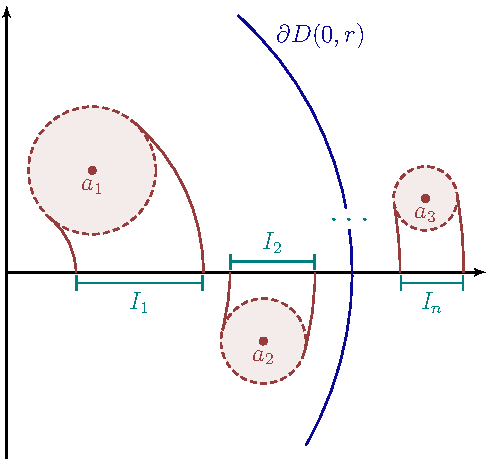
\includegraphics{%
                Figuras/In Hadamard.pdf
            }
        \end{figure}
        %
        Ora, mas a união dos $I_n$ não pode cobrir $[L, L+1]$ já que
        %
        \begin{align*}
            \Leb\left(
            \bigcup_{n=n_0}^{\infty} I_n
            \right) 
            \leq
            \sum_{n=n_0}^{\infty} \Leb(I_n)
            =
            \sum_{n=n_0}^{\infty} \frac{2}{|a_n|^{k+1}}
            <
            \frac{2}{10},
        \end{align*}
        %
        enquanto que $\Leb([L, L+1]) = 1$. Portanto, podemos encontrar 
        a sequência desejada $(r_n)_{n\in\N}$ com $r_n \xrightarrow{n\to\infty} \infty$
        aplicando o Lema \ref{lema:5.3-Stein}.
    \end{proof}
    %
    
    \medskip
    
    Antes de rumar para a demonstração do teorema de Hadamard, vamos precisar de um último
    lema.
    %
    \begin{lema}
    \label{lema:5.5-Stein}
        Seja $g:\C\to\C$ uma função inteira tal que, para algum $s>0$,
        %
        \begin{equation*}
            \Re(g(z)) \leq C r^s
        \end{equation*}
        %
        sempre que $|z| = r$ para uma sequência de números reais positivos $r$ que tende para o infinito.
        Então $g$ é um polinômio de grau menor ou igual a $s$.
    \end{lema}
    %
    \begin{proof}
        Expandindo $g$ em série de potências ao redor da origem, temos
        %
        \begin{equation*}
            g(z) = \sum_{n=0}^{\infty} a_n z^n.
        \end{equation*}
        %
        Observe que $a_k = g^{(k)}(0)/k!$. Usando a fórmula integral de Cauchy e lembrando como as derivadas de $g$ se expressam por meio desta fórmula, temos que, para $n \geq 0$,
        %
        \begin{align*}
            a_n = \frac{g^{(n)}(0)}{n!} &= \frac{1}{2\pi i} \int_{\partial D_r} \frac{g(w)}{(w - 0)^{n+1}} \, dw \\
            &= \frac{1}{2\pi r^n} \int_{0}^{2\pi} g(re^{i\theta})e^{-in\theta} \, d\theta.
        \end{align*}
        %
        A mesma identidade vale para $n < 0$, mas, nesse caso a integral se anula, pois $g(w)/w^{n+1} = g(w)w^{-n-1}$ é holomorfa. Concluímos, então, que
        \begin{equation*}
            \frac{1}{2\pi} \int_0^{2\pi} g(re^{i\theta}) e^{-in\theta} \, d\theta
            =
            \begin{cases}
                a_n r^n, n \geq 0 \\
                0, n < 0
            \end{cases}.
        \end{equation*}
        %
        Tomando conjugados complexos, obtemos
        %
        \begin{equation*}
            \frac{1}{2\pi} \int_0^{2\pi} \overline{ g(re^{i\theta}) } e^{-in\theta} \, d\theta = 0
        \end{equation*}
        %
        sempre que $n > 0$. Como $2\Re(g) = g + \overline{g}$, adicionamos as duas equações
        acima para obter
        %
        \begin{equation*}
            a_n r^n = \frac{1}{\pi} \int_0^{\pi} \Re(g(re^{i\theta}))e^{-in\theta} \, d\theta,
            \, n > 0.
        \end{equation*}
        %
        Para $n = 0$, tomamos a parte real em ambos os lados da primeira integral para encontrar
        %
        \begin{equation*}
            2\Re(a_0) = \frac{1}{\pi}\int_0^{2\pi} \Re(g(re^{i\theta})) \, d\theta.
        \end{equation*}
        %
        Agora, notamos o fato de que para todo $n\neq 0$ a integral de $e^{-in\theta}$
        em qualquer circunferência de centro na origem é nula. Portanto,
        %
        \begin{equation*}
            a_n 
            = 
            \frac{1}{\pi r^n} \int_0^{2\pi} \left[ \Re(g(re^{i\theta})) - Cr^s \right]e^{-in\theta}
            \, d\theta, \, n > 0,
        \end{equation*}
        %
        e segue que
        %
        \begin{equation*}
            |a_n| 
            \leq
            \frac{1}{\pi r^n} 
            \int_0^{2\pi} \left[ Cr^s - \Re(g(re^{i\theta})) \right] \, d\theta
            \leq
            2Cr^{s-n} - 2\Re(a_0)r^{-n}.
        \end{equation*}
        %
        Fazendo $r\to\infty$, obtemos que $a_n = 0$ para $n > s$, de modo que $g$
        é um polinômio de grau no máximo $s$, como desejado.
    \end{proof}
    %
    
    \medskip
    
    Agora, para provar o teorema de Hadamard, seja
    %
    \begin{equation*}
        E(z) = z^m \prod_{n=1}^{\infty} E_k(z/a_n).
    \end{equation*}
    %
    Para mostrar que $E$ é inteira, aplicamos a Proposição \ref{prop:prod-inf-func-holom} notando que
    %
    \begin{equation*}
        |1 - E_k(z/a_n)| \leq c\left| \frac{z}{a_n} \right|^{k+1}
    \end{equation*}
    %
    para todo $n$ suficientemente grande (como no Lema \ref{lema-wstr-est-factor}) e também que
    %
    \begin{equation*}
        \sum_{n=0}^{\infty} \frac{1}{|a_n|^{k+1}}
    \end{equation*}
    %
    converge, pois $\rho_0 < s < k+1$, . Além disso, $E$ tem os mesmos zeros 
    que $f$, de modo que $f/E$ é holomorfa e não se anula em lugar nenhum,
    ou seja,
    %
    \begin{equation*}
        \frac{f(z)}{E(z)} = e^{g(z)}
    \end{equation*}
    %
    para alguma função inteira $g$. Como $f$ tem ordem de crescimento
    $\rho_0$ e pela estimativa para $E$ obtida no Corolário \ref{cor-seq-raios-inf},
    temos
    %
    \begin{align*}
        \exp(\Re(g(z))) &= \left| \frac{f(z)}{E(z)} \right| \\
                        &\leq \frac{A_1 \exp( B_1|z|^{\rho_0} )}{A_2 \exp( -B_2|z|^{s} )} \\
                        &= A_1 \exp(B_1 |z|^{\rho_0} + B_2 |z|^s) \\
                        &\leq A_1 \exp(B_3 |z|^s).
    \end{align*}
    %
    para $|z| = r_m$. Isso mostra que
    %
    \begin{equation*}
        \Re(g(z)) \leq A_2|z|^s, \, |z| = r_m
    \end{equation*}
    %
    e segue do Lema \ref{lema:5.5-Stein} que $g$ é um polinômio de grau menor
    ou igual a $s$, terminando a demonstração.
    %
    % falar do teo de Mittag-Leffler e da aplicação para funções com imagens prescritas (?)
 
 
 
 
 
    \subsection{O Pequeno Teorema de Picard}
    
    Nesta seção vamos mostrar, como consequência do Teorema de Hadamard, um resultado fascinante devido a Picard. Ele afirma, entre outras coisas, 
    que a imagem de uma função inteira, de ordem de crescimento finita, pode omitir no máximo um ponto do plano complexo! 
    Isto é, se $f:\C\to\C$ é uma função inteira com ordem de 
    crescimento $0\leqslant \rho<+\infty$, então a o conjunto imagem $f(\C)$ 
    é todo o plano complexo, exceto por, possivelmente, um ponto.
    Este resultado é conhecido como o {\it Pequeno Teorema de Picard}. Seu enunciado mais preciso é apresentado logo abaixo.
 
    
        %
        \begin{teorema}[Pequeno Teorema de Picard]
        \label{teo:pequeno-picard}
        \index{Pequeno Teorema de Picard}
            Se $f:\C\to\C$ é uma função inteira não constante e com ordem de crescimento 
            $\rho \in [0,+\infty)$, então
            %
            \[
              \sharp (f(\C))^c \leq 1.
            \]
            %
            Além do mais,
            \begin{itemize}
                \item se $0\leqslant \rho<1$, então $f(\C)=\C$; 
                
                \item se $1\leqslant \rho<+\infty$, então 
                a imagem de $f$ omite no máximo um ponto do plano complexo 
                e todo ponto da imagem de $f$ possui infinitas pré-imagens.
            \end{itemize}
        \end{teorema}

        \medskip 
        %
        Antes de apresentar a prova do Teorema de Picard vamos enunciar um pequeno lema preliminar, um corolário do Teorema Fundamental da Álgebra.
        
        \medskip 
        %
        \begin{lema}
        \label{lema-pol-sobrejetor}
            Todo polinômio não constante $P:\C\to\C$ é sobrejetor.
        \end{lema}
        %
        \begin{proof}[Demonstração do lema]
            Dado $w\in\C$, o polinômio $P(z) - w$ é não constante e, pelo
            Teorema Fundamental da Álgebra, tem uma raiz $z_w$. Ora, então
            $P(z_w) = w$ e, portanto, $P$ é sobrejetor.
        \end{proof}
        
        \medskip
        %
        Vamos, então, à demonstração do Pequeno Teorema de Picard.
        %
        \begin{proof}[Demonstração do Pequeno Teorema de Picard]
            Suponha que existe algum $a\in\C$ tal que
            %
            \[
            f(z) - a \neq 0, \quad \forall z\in\C.
            \]
            %
            Em outras palavras, estamos supondo que a função inteira $g:\C\to\C$ 
            dada por $g(z)= f(z)-a$ não possui raízes. 
            Observe que $g$ é uma função inteira de ordem de crescimento 
            finito $\rho$. Portanto, podemos aplicar o Teorema da 
            Fatoração de Hadamard (Teorema \ref{teo:fatoracao-hadamard}) 
            para garantir que 
            %
            \begin{align}
            \label{eq-aux1-litle-picard}
                f(z) - a = e^{P(z)},
            \end{align}
            %
            onde $P(z)$ é um polinômio de grau no máximo $\rho$.
            
            \medskip 
            Vamos separar o restante do argumento em dois casos.
            \begin{itemize}
                \item Caso 1. $0\leqslant \rho<1$;
                \item Caso 2. $1\leq\rho<+\infty$.
            \end{itemize}
            \medskip 
            
            
            Caso 1. Neste caso, como $0\leqslant \rho<1$, então  
            segue do Teorema da Fatoração de Hadamard que
            o polinômio que aparece no lado direito de
            \eqref{eq-aux1-litle-picard} é tal que
            $\textrm{grau}(P)=\lfloor \rho \rfloor =0$, ou seja, 
            $P$ é constante. Mas então existe 
            alguma constante $K\in \C$ tal que 
            $f(z)-a=e^K$ para todo $z\in\C$, o que 
            é um absurdo, pois por hipótese 
            $f$ é não-constante. 
            
            O absurdo vem de termos assumido que existe um número complexo $a$ tal que a função $g=f-a$ não possui raízes. Desta forma, para todo $a\in\C$ fixado, existe algum $z\in \C$ 
            tal que $f(z)=a$ e, portanto, $f(\C)=\C$.
            
            
            \bigskip
            Caso 2.
            Neste segundo caso, sabemos que $P$ tem grau no máximo
            $\rho \geq 1$. Se, por ventura, $P$ for constante,
            então voltamos ao caso anterior.
            
            Assumamos então $P$ não constante.
            Já que todo ponto não-nulo do plano complexo
            pode ser representado em coordenadas polares, podemos afirmar que dado um ponto arbitrário 
            $b\in \C\setminus\{a\}$,
            existe algum $\varphi \in [0, 2\pi)$ tal que
            %
            \[
            b - a = |b - a| e^{i\varphi}.
            \]
            %
            Usando o Lema \ref{lema-pol-sobrejetor},
            podemos garantir que existe um número complexo $z_b\in\C$ tal que
            %
            \begin{align*}
                P(z_b) = \ln|b-a| + i\varphi.
            \end{align*}
            %
            Substituindo $z$ por $z_b$ em
            \eqref{eq-aux1-litle-picard} e usando a igualdade acima ficamos com
            %
            \[
            f(z_b) - a = b - a 
            \qquad \iff \qquad f(z_b) = b.
            \] 
            %
            Consequentemente, a  
            imagem do $f$ pode omitir 
            no máximo um ponto de $\C$.
            
            Para mostrar que a imagem inversa de qualquer ponto 
            $b\in \C\setminus\{a\}$ possui infinitos pontos, basta 
            observar que para cada $k\in\Z$, podemos usar 
            novamente o Lema \ref{lema-pol-sobrejetor}
            para garantir que existe um ponto 
            $z_{b,k}\in \C$
            tal que 
            \begin{align*}
                P(z_{b,k}) = \ln|b-a| + i(\varphi+2k\pi).
            \end{align*}
            Argumentando de maneira análoga, 
            concluímos que 
            $f(z_{b,k})=b$. 
            Já que para qualquer par de inteiros distintos $k$ e $k'$
            temos $z_{b,k}\neq z_{b,k'}$, pois 
            $\Im(P(z_{b,k}))\neq \Im(P(z_{b,k'}))$, 
            segue que $b$ tem infinitas pré-imagens. 
            Como $b\in \C\setminus\{a\}$
            é arbitrário, finalizamos a prova do teorema.
        \end{proof}
        %
        
        
        
\section{A função Gama}

    O fatorial é uma aplicação conhecida de todos que, para cada inteiro não negativo $n$ 
    associa $n! \equiv n \cdot (n-1) \cdots 3 \cdot 2 \cdot 1$ e convenciona-se $0! = 1$. 
    Podemos expressar os fatoriais como integrais reais por meio da identidade
    %
    \[ 
    (n-1)! = \int_0^{\infty}e^{-t} t^{n-1} \, dt.
    \]
    %
    Nesta seção, vamos estudar a função Gama, que será denotada por $\Gamma$. Ela é uma função de grande importância na Análise 
    Matemática e na Teoria Analítica dos Números. 
    Esta função pode ser vista como uma extensão 
    do conceito de fatorial de um número natural. 
    Para cada $s>0$, definimos
    %
    \begin{align}
        \label{def-func-gamma-real}
    \Gamma(s) \equiv \int_0^{\infty}e^{-t} t^{s-1} \, dt.
    \end{align}
    %
    Primeiro, vamos mostrar que $\Gamma$ está bem definida. Problemas de convergência 
    podem ocorrer quando $t = 0$ e $s - 1 < 0$ e também conforme $t$ toma valores muito grandes.
    
    Observe que $s - 1 < 0$ ocorre somente se $0 < s < 1$. Vamos mostrar que a integral 
    de 0 a 1 é limitada. Seja $\e > 0$ qualquer, então
    %
    \begin{align*}
        \left| \int_{\e}^{1}e^{-t}t^{s-1} \, dt \right| 
        &\leq \int_{\e}^{1}t^{s-1} \, dt \\[0.3cm]
        &= \frac{t^s}{s}\Big |_{\e}^{1} \\[0.3cm]
        &= \frac{1}{s} - \frac{\e^s}{s} \xrightarrow{\ \e\to 0\ } \frac{1}{s}.
    \end{align*}
    %
    Esta simples estimativa mostra a razão de escolhermos $s > 0$. 
    No entanto, isto não mostra completamente o por quê desta escolha.
    O segundo motivo é que, se $s = -\delta < 0$, então
    %
    \begin{align*}
        \int_{\e}^{1}e^{-t}t^{s-1} \, dt &= \int_{\e}^{1}e^{-t}t^{-1-\delta} \, dt \\[0.3cm]
        &\geq \int_{\e}^{1}t^{-1-\delta} \, dt \\[0.3cm]
        &= \frac{t^{-\delta}}{\delta}\Big |_{t = \e}^{1} \\[0.3cm]
        &= \frac{\e^{-\delta}}{\delta} - \frac{1}{\delta} \xrightarrow{\ \e\to 0\ } \infty.
    \end{align*}
    %
    
   
    
    Analisamos agora a outra porção da integral. Primeiro, observe que $e^{-t/2}t^{s-1}$ 
    vai a 0 conforme $t$ cresce. Isto mostra que esta expressão é limitada. Então
    %
    \begin{align*}
        \int_{1}^{1/\e}e^{-t}t^{s-1} \, dt &\leq M\int_{\e}^{1}e^{-t/2} \, dt \\[0.3cm]
        &= 2M(e^{-1/2} - e^{-1/2\e}) < \infty
    \end{align*}
    %
    para todo $\e > 0$. 
    Estas considerações mostram que a função $\Gamma$ está bem 
    definida para todo $s > 0$.
    
    O nosso objetivo é estender $\Gamma$ para todo o plano complexo. 
    Tentaremos realizar tal extensão admitindo que $s$ seja um número complexo. 
    Inicialmente, consideraremos o semiplano $\Re(s) > 0$.
    
    
    \begin{lema}
    \label{lema-conv-abs-cond-int-imp}
        Sejam $\Omega \subseteq \C$ um domínio e 
        $f: \Omega \times (0,\infty)\to \C$ uma função. 
        Assuma que para cada $z \in \Omega$ fixado, 
        que o conjunto de descontinuidades da função 
        $t \mapsto f(z,t)$ tenha medida de Lebesgue nula. 
        Além disso, assuma que para $z\in \Omega$ fixado e cada $\delta>0$ dado que 
        %
        \[
        \sup_{t \in [\delta,1/\delta]} |f(z,t)| < \infty.
        \]
        %
        Se $z\in \Omega$ fixado é tal que o seguinte limite existe
        %
        \[
        \lim_{\delta \to 0} 
        \int_{\delta}^{ \frac{1}{\delta} }
        |f(z,t)| \, dt
        \equiv 
        \int_{0}^{\infty} |f(z,t)|\, dt ,
        \]
        %
        então para cada $z\in\Omega$, existe o limite 
        %
        \[
        g(z) \equiv \lim_{\delta \to \infty} 
        \int_{\delta}^{ \frac{1}{\delta} }f(z,t) \, dt
        \equiv
        \int_{0}^{\infty }f(z,t) \, dt.
        \]
        %
    \end{lema}
    %
    \begin{proof}
        Fixado $z\in \Omega$ e dado $\delta>0$ temos diretamente
        das hipóteses do lema que a integral abaixo existe e é finita
        %
        \[
        \int_{\delta}^{ \frac{1}{\delta}  }|f(z,t)| \, dt.
        \]
        %
        Além disso, por hipótese temos garantia da existência do seguinte
        limite:
        %
        \[
        I \equiv \lim_{\delta \to \infty} 
        \int_{\delta}^{ \frac{1}{\delta} }|f(z,t)| \, dt.
        \]
        % 
        Isto significa que, dado $\e > 0$ qualquer, existe 
        $\delta_0\equiv \delta_0(\varepsilon,z) > 0$ tal que, para todo
        $0<\delta < \delta_0$  temos
        %
        \[
        \Big | I - \int_{\delta}^{ \frac{1}{\delta} }|f(z,t)| \, dt \Big | < \e.
        \]
        %
        Usando a desigualdade triangular 
        podemos verificar que para quaisquer par de
        números reais $\rho$ e $\delta$ satisfazendo
        $0<\rho,\, \delta <\delta_0$, temos
        %
        \begin{align}
        \label{eq-aux1-lema-conv-abs-cond-int-imp}
        \left| 
            \int_{\rho}^{ \frac{1}{\rho} }|f(z,t)| \, dt
            -
            \int_{\delta}^{ \frac{1}{\delta} }|f(z,t)| \, dt
        \right| 
        &= 
        \left| 
            \int_{\rho}^{ \frac{1}{\rho} }|f(z,t)| \, dt - I
            +
            I -\int_{\delta}^{ \frac{1}{\delta} }|f(z,t)| \, dt
        \right|
        \nonumber\\[0.3cm]
        &\leqslant
        \left| 
            I- \int_{\rho}^{ \frac{1}{\rho} }|f(z,t)| \, dt 
        \right|
        +
        \left| 
            I -\int_{\delta}^{ \frac{1}{\delta} }|f(z,t)| \, dt
        \right|
        \nonumber\\[0.3cm]
        &<
        2\e.
        \end{align}
        %
        Seja $(a_n)_{n\in\N}$ uma sequência arbitraria de números reais estritamente positivos tal que 
        $a_n\to 0$, quando $n\to\infty$ e defina para cada $n\in\N$
        %
        \[
        I_n  
        \equiv 
        I_n(z) 
        \equiv
        \int_{ a_n }^{ \frac{1}{a_n} }f(z,t) \, dt.
        \]
        %
        Como $(a_n)_{n\in \N}$ é uma sequência arbitrária
        tudo que precisamos para finalizar a prova do lema é mostrar que a sequência $(I_n)_{n\in\N}$ é uma sequência de Cauchy e, em seguida,
        mostrar que o limite desta sequência é independente da escolha
        particular de $(a_n)_{n\in \N}$. 
        
        Já que $a_n\to 0$, quando $n\to\infty$, sabemos que dado 
        $\e>0$, existe $n_0\in\N$ tal que para todo $n,m\geqslant n_0$
        temos $0< a_n,\, a_m <\delta_0$. Portanto segue diretamente da desigualdade \eqref{eq-aux1-lema-conv-abs-cond-int-imp}
        que 
        \begin{align*}
            |I_n - I_m| 
            = 
            \left| 
            \int_{a_n}^{ \frac{1}{a_n} }f(z,t) \, dt 
            - \int_{ a_{m} }^{ \frac{1}{a_m} }f(z,t) \, dt 
            \right|
            <2\e.
        \end{align*}
        %
        O que mostra que $(I_n)_{n\in\N}$ é uma sequência de Cauchy
        e consequentemente uma sequência convergente. 
        Denote por $J$ o limite desta sequência. 
        A rigor, observamos que o valor deste limite poderia depender 
        da particular escolha da sequência $(a_n)_{n\in\N}$. 
        Mas aqui este não é o caso e para suportar esta afirmação  
        vamos mostrar que este limite é o 
        mesmo para qualquer sequência de número reais positivos 
        que converge para zero. 
        
        Suponha que $J_1, J_2$ são limites obtidos usando 
        duas sequências distintas de números reais positivos que convergem para zero, digamos $(a_n)_{n\in\N}$ e $(b_n)_{n\in\N}$,
        respectivamente. 
        
        Nestas condições, dado $\e>0$ podemos encontrar $n_0\in\N$ tal 
        que para todo $n\geqslant n_0$ temos
        $0<a_n,\ b_n <\delta_0$ e também
        \[
        \left|J_1-\int_{a_n}^{ \frac{1}{a_n} }f(z,t) \, dt \right|<\e
        \qquad\text{e}\qquad
        \left|J_2-\int_{b_n}^{ \frac{1}{b_n} }f(z,t) \, dt \right|<\e.
        \]
        
        Usando a desigualdade triangular, 
        as três últimas desigualdades acima e em seguida a desigualdade \eqref{eq-aux1-lema-conv-abs-cond-int-imp}
        podemos concluir que 
        %
        \begin{align*}
            |J_1& - J_2| 
            \\[0.3cm]
            &= 
            \left| 
            J_1-\int_{a_n}^{ \frac{1}{a_n} }f(z,t) \, dt 
            +\int_{a_n}^{ \frac{1}{a_n} }f(z,t) \, dt 
            - \int_{ b_{n} }^{ \frac{1}{b_n} }f(z,t) \, dt
            +
             \int_{ b_{n} }^{ \frac{1}{b_n} }f(z,t) \, dt
             -J_2
            \right| 
            \\[0.3cm]
            &\leqslant
            \left| 
            J_1-\int_{a_n}^{ \frac{1}{a_n} }\!\! f(z,t) \, dt 
            \right|
            +
            \left|
            \int_{a_n}^{ \frac{1}{a_n} }\!\! f(z,t) \, dt 
            - \int_{ b_{n} }^{ \frac{1}{b_n} }\!\! f(z,t) \, dt
            \right|
            +
            \left|
             \int_{ b_{n} }^{ \frac{1}{b_n} }\!\!\! f(z,t) \, dt
             -J_2
            \right|
            \\[0.3cm]
            &<4\e.
        \end{align*}
        %
       Como $\e>0$ na desigualdade acima é arbitrário, 
       temos obrigatoriamente $J_1=J_2$. 
       Com isto encerramos a prova do lema.
    \end{proof}
    %
    \begin{observacao}
        No lema anterior, assumimos que a função $f$ com $z$ fixado tem um conjunto de descontinuidades com medida de Lesbegue nula, isto é equivalente a dizer que ela é Riemann integrável 
        em relação à variável $t$ real. Além disso, vale um resultado análogo ao anterior: Se assumimos que existe 
        %
        \[
        \lim_{a \to \infty} \int_{-a}^{a}|f(z,t)| \, dt,
        \]
        %
        então podemos mostrar similarmente que existe
        %
        \[
        \lim_{a \to \infty} \int_{-a}^{a}f(z,t) \, dt.
        \]
        %
    \end{observacao}
    
    
    \bigskip 
    
    
    Seja $s \in \C$ e denote $\sigma = \Re(s)$. Então 
    para todo $t>0$ temos que 
    %
    \begin{align*}
        |t^{s-1}| &= |\exp((s-1)\ln t)| \\
        %
        &= \exp(-\ln{t})|\exp(s\ln t)| \\
        %
        &= \exp(-\ln{t})|\exp(\sigma\ln t)| \\
        %
        &= t^{\sigma - 1}.
    \end{align*}
    %
    Além do mais, para qualquer $\delta>0$ dado,
    temos as seguinte estimativa
    \[
    \sup_{t\in [\delta,1/\delta]} |e^{-t}t^{s-1}|
    =
    \sup_{t\in [\delta,1/\delta]} e^{-t}t^{\sigma-1}
    <+\infty.
    \]
    %
    Tomando $\sigma=\Re(s)>0$ temos também que 
    \begin{equation*}
        \int_{0}^{\infty}|e^{-t}t^{s-1}| \, dt = \int_{0}^{\infty}e^{-t}|t^{s-1}| \, dt = \int_{0}^{\infty}e^{-t}t^{\sigma-1} \, dt 
        = 
        \Gamma(\sigma)<+\infty,
    \end{equation*}
    %
    Seja $\Omega\equiv \{s\in\C: \Re(s)>0\}$. 
    Já que a aplicação $f:\Omega\times (0,\infty)\to\C$ dada por 
    $f(s,t)= e^{-t}t^{s-1}$ é contínua, segue 
    das observações acima que podemos aplicar o lema anterior para 
    provar que existe
    %
    \[
    \Gamma(s)\equiv \int_{0}^{\infty}e^{-t}t^{s-1} \, dt,
    \]
    para todo $s\in\C$ tal que $\Re(s)>0$. 
    %
    \begin{teorema}
        A função $\Gamma:(0,\infty)\to\R$ definida em \eqref{def-func-gamma-real}
        admite uma extensão analítica para o semiplano 
        $\{s \in \C : \Re(s) >0 \}$ e além do mais para qualquer ponto
        $s$ neste semi-plano esta extensão analítica é representada pela
        seguinte integral 
        \[
        \Gamma(s)\equiv \int_{0}^{\infty}e^{-t}t^{s-1} \, dt
        \]
    \end{teorema}
    %
    \begin{proof}
        Naturalmente, a função que é candidata a ser a extensão de $\Gamma(s)$ 
        é aquela que tem a mesma expressão, mas em que admitimos que a variável $s$ seja complexa.
        Aqui, por abuso de linguagem, denotaremos esta candidata por $\Gamma(s)$ também. Sejam 
        $
        0 < \delta < M$ quaisquer números reais positivos fixados e 
        considere a faixa $S\equiv  S_{\delta, M} 
        \equiv 
        \{ s \in \C : \delta < \Re(s) < M\}$. 
        Vamos mostrar, para quaisquer escolhas das constantes $\delta$ e $M$, que a função $s\longmapsto\Gamma(s)$ definida na faixa $S$ é o limite uniforme da sequência de funções $(g_n)_{n\in \N}$, onde
        %
        \[
        g_n(s) = \int_{1/n}^{n}e^{-t}t^{s-1} \, dt.
        \]
        %
        Vamos mostrar também que $g_n$ é uma função holomorfa,
        para cada $n\in \N$ e concluir então que $\Gamma$ é holomorfa na faixa $S$. 
        
        Para provar as afirmações feitas acima, vamos começar mostrando que para cada $n\in \N$ fixado que $g_n:S\to C$ é uma função contínua. De fato, seja $s_0 \in S$ temos  
        %
        \begin{align*}
            |g_n(s)-g_n(s_0)|
            &=
            \left|
            \int_{1/n}^{n}e^{-t}t^{s-1} \, dt
            -
            \int_{1/n}^{n}e^{-t}t^{s_0-1} \, dt
            \right|
            \\[0.3cm]
            &\leqslant
            \int_{1/n}^{n} |t^{s-1}-t^{s_0-1}| \, dt
            \\[0.3cm]
            &\leqslant
            \int_{1/n}^{n}
            \frac{1}{t} |t^{s}-t^{s_0}|            
            \, dt
            \\[0.3cm]
            &\leqslant
            n
            \int_{1/n}^{n}
            |t^s-t^{s_0}| \, dt.
        \end{align*}
        %
    
    Observe agora que a aplicação $s \mapsto t^s = \exp(s\ln t)$ é contínua e $ I_n = [1/n, n]$ é compacto, então podemos encontrar $\delta > 0$ tal que $\sup_{t \in I_n} |t^s-t^{s_0}| < \e/n^2$ quando $|s - s_0| < \delta$. Para verificar isto note que, fixado $t \in I_n$ e dado $\e/n^2 > 0$, encontramos $\delta_t > 0$ tal que $|t^s - t^{s_0}| < \e/n^2$ sempre que $|s - s_0| < \delta_t$. Como $t \mapsto t^s$ também é contínua, há uma vizinhança $B_t = (t-\xi_t, t+ \xi_t)$ de $t$ em que ainda vale a mesma estimativa. As bolas $B_t$ formam uma cobertura de $I_n$ por abertos, então, por compacidade, há uma subcobertura finita com centros $t_1, t_2, \dots, t_r$. Seja $\delta = \min\{\delta_{t_1}, \dots, \delta_{t_r}\}$, então $|s - s_0| < \delta$ implica que $|t^s-t^{s_0}| < \e/n^2$ para todo $t \in I_n$, ou seja, $\sup_{t \in I_n} |t^s-t^{s_0}| < \e/n^2$. 
    
    Com esta estimativa, temos 
    %
    \begin{align*}
        |g_n(s)-g_n(s_0)| &\leq n
            \int_{1/n}^{n}
            |t^s-t^{s_0}| \, dt\\
            %
            &\leq n \frac{\e}{n^2}\int_{1/n}^{n} \, dt \\
            %
            &= n\left(n-\frac{1}{n}\right)\frac{\e}{n^2} \\
            %
            &\leq \e.
    \end{align*}
    %
    Isto mostra que as $g_n$ são funções contínuas.
        
    Próximo passo é mostrar que a integral de $g_n$ ao longo de qualquer
    triângulo contido em $S$ é nula. 
    Para isto, seja $\Delta$ um triângulo arbitrário, contido em $S$. 
    Como a função no integrando que define $g_n$ é contínua, 
    segue do Teorema de Fubini que
        %
        \begin{align*}
            \int_{\Delta}g_n(s)\, ds &= \int_{\Delta}\int_{1/n}^{n}e^{-t}t^{s-1} \, dt \, ds \\
            &= \int_{1/n}^{n} \int_{\Delta} e^{-t}t^{s-1} \, ds \, dt  \\
            &= \int_{1/n}^{n} 0 \, dt = 0.
        \end{align*}
        %
        Já que $\Delta$ é um triângulo qualquer em $S$ e $g_n$ é contínua segue finalmente do Teorema de Morera que $g_n$ é holomorfa.
        
        
        
    \bigskip 
    
    Vamos mostrar agora que $g_n$ converge uniformemente,
    quando $n\to\infty$, para $\Gamma$. De fato, dado qualquer
    $s\in S$ temos 
        %
        \begin{align*}
            |\Gamma(s) - g_n(s)| &= \Big | \int_{0}^{\infty}e^{-t}t^{s-1} \, dt -  \int_{1/n}^{n}e^{-t}t^{s-1} \, dt \Big | \\
            %
            & = \Big | \int_{0}^{1/n}e^{-t}t^{s-1} \, dt +  \int_{n}^{\infty}e^{-t}t^{s-1} \, dt \Big | \\
            %
            &\leq \Big | \int_{0}^{1/n}e^{-t}t^{s-1} \, dt \Big | +  \Big | \int_{n}^{\infty}e^{-t}t^{s-1} \, dt \Big | \\
            %
            &\leq \int_{0}^{1/n}e^{-t}|t^{s-1}| \, dt  + \int_{n}^{\infty}e^{-t}|t^{s-1}| \, dt \\
            %
            &\leq \int_{0}^{1/n}t^{\sigma-1} \, dt + \int_{n}^{\infty}e^{-t}t^{\sigma-1} \, dt \\
            %
            &\leq \int_{0}^{1/n}t^{\delta-1} \, dt + \int_{n}^{\infty}e^{-t}t^{M-1} \, dt \\
            %
            &\leq \frac{1}{\delta}\frac{1}{n^\delta} + K_M\int_{n}^{\infty}e^{-t/2} \, dt.
        \end{align*}
        %
        Já que o lado direito da estimativa acima vai a zero,
        quando $n\to\infty$, independentemente da escolha de $s\in S$, segue que $\Gamma(s)$ é holomorfa na faixa 
        $S$ \textcolor{red}{(citar teorema)}. 
        Lembrando que as constantes $M$ e $\delta$ são arbitrárias, 
        podemos concluir que $\Gamma(s)$ é holomorfa em todo $U$.
    \end{proof}
    
    
    \bigskip 
    
    A seguir, mostramos que a função Gama satisfaz uma equação funcional.
    Esta equação funcional será usada para revelar diversas propriedades 
    da função Gama, que não são simples de serem obtidas à partir 
    de sua definição.
    Vamos usá-la para dar uma prova de que função Gama pode ser estendida à 
    função meromorfa em $\C$ bem como para determinar os resíduos 
    de Gama em cada uma de suas singularidades.  
    %
    
    
    Apesar de toda sua aplicabilidade e incríveis consequências a equação funcional pode ser obtida por uma simples aplicação do método de integração por partes, como mostramos a seguir. 
    
    Pela regra do produto, temos que
    %
    $$\frac{d}{dt}(e^{-t}t^{s}) = se^{-t}t^{s-1} - e^{-t}t^{s}.$$
    %
    Considerando que $s$ satisfaz $\Re(s)>0$, integrando ambos os lados da igualdade acima e usando o Teorema Fundamental do Cálculo obtemos
    %
    \begin{align*}
        0 
        &= 
        \lim_{\e \to 0^+} e^{-t}t^s \Big|_{\e}^{1/\e} 
        \\[0.3cm]
        %
        &= 
        \lim_{\e \to 0^+} s\int_{\e}^{1/\e} e^{-t}t^{s-1} \, dt - \int_{\e}^{1/\e} e^{-t}t^{s} \, dt 
        \\[0.3cm]
        %
        &= 
        s\Gamma(s) - \Gamma(s+1).
    \end{align*}
    %
    Portanto, fica demonstrado o seguinte teorema.
    
    \begin{teorema}\label{teo-eq-func-Gama}
    Se $\Re(s)>0$, então $\Gamma(s+1) = s\Gamma(s)$.
    \end{teorema}

    Note que podemos concluir do teorema 
    acima a validade da afirmação feita 
    no início desta seção, isto é, 
    $\Gamma(n) = (n-1)!$, 
    para todo $n > 0$ inteiro. 
    
    \begin{teorema}
    \label{teo-cont-meromorfa-gamma}
        A função $\Gamma$, inicialmente definida para $\Re(s) > 0$, admite uma continuação analítica à uma função meromorfa em $\C$ com polos simples nos inteiros não positivos. Além disso, o resíduo em $-n$ é $(-1)^{n}/n!$ para todo $n \in \N \cup \{0\}$.
    \end{teorema}
    \begin{proof}
    Para cada $m \in \N$, defina 
    \[
    U_m = \{s \in \C \setminus \{0,-1, \dots, -(m-1)\}: \Re(s) > -m \}.
    \]
    Vamos definir a continuação de $\Gamma$ por etapas, primeiro a estendemos para $U_1$, depois para $U_2$ e assim sucessivamente. Seja $F_1 : U_1 \to \C$ dada por
    %
    $$F_1(s) = \frac{\Gamma(s+1)}{s}.$$
    %
    Quando $\Re(s) > 0$, podemos concluir da equação funcional de $\Gamma$ que 
    %
    $$F_1(s) = \frac{s\Gamma(s)}{s} = \Gamma(s),$$
    %
    logo, $F_1$ e $\Gamma$ coincidem neste semiplano. Em particular, $F_1$ é holomorfa porque é definida a partir de $\Gamma$ e, quando $\Re(s)> -1$, temos $\Re(s+1) > 0$. Observe ainda que
    %
    $$ \lim_{s \to 0} sF_1(s) = \Gamma(1) = 1 \neq 0,$$
    %
    então $s=0$ é um polo simples de $F_1$ com resíduo neste ponto sendo igual à $1$.
    
    Definimos agora a função holomorfa $F_2 : U_2 \to \C$ 
    pela seguinte expressão
    %
    $$F_2(s) = \frac{\Gamma(s+2)}{s(s+1)}.$$
    %
    Quando $\Re(s) > -1$, podemos usar a equação funcional e observar que $F_2(s) = F_1(s)$ neste semiplano. Além disso, 
    %
    $$ \lim_{s \to -1} (s+1)F_2(s) = \lim_{s \to -1} \frac{\Gamma(s+2)}{s} = \frac{\Gamma(1)}{-1} = -1 \neq 0$$
    %
    e temos $\res(F_2,-1) = -1$. 
    
    Continuamos deste modo definindo $F_{n+1} : U_{n+1} \to \C$ por
    %
    $$F_{n+1}(s) = \frac{\Gamma(s+n+1)}{(s+n)(s+n-1) \cdots (s+1)s}.$$
    %
    Como anteriormente, esta função também é holomorfa e temos
    %
    \begin{align*}
        \lim_{s \to -n} (s+n)F_{n+1}(s) &= \lim_{s \to -n} (s+n)\frac{\Gamma(s+n+1)}{(s+n)(s+n-1) \cdots (s+1)s} \\
        &= \frac{\Gamma(1)}{(-1)(-2) \cdots [-(n-1)](-n)} = \frac{(-1)^n}{n!}
    \end{align*}
    %
    mostrando que $F_{n+1}$ tem um polo simples em $s=-n$ e que o resíduo desta função neste polo é exatamente $(-1)^n/n!$. 
    
    Usando os fatos demonstrados acima podemos definir a função $\Gamma$ em todo conjunto $\C\setminus \{0,-1,-2,-3,\ldots\}$
    da seguinte forma. 
    Dado $s\in \C\setminus \{0,-1,-2,-3,\ldots\}$ seja $n\in \N$
    o menor natural tal que $s\in U_n$ e defina $\Gamma(s) \equiv F_n(s)$. Observe que Gama definida assim é uma função bem definida e além do mais todas suas singularidades, 
    isto é, os pontos do conjunto $\{0,-1,-2,-3,\ldots$ são pontos isolados e todos são também polos simples de $\Gamma$ com resíduos dados por 
    \[
    \mathrm{res}(\Gamma,-n) = \frac{(-1)^n}{n!}.
    \]
    \end{proof}
    
    
    
    \begin{corolario}
    \label{cor-eq-func-Gamma}
    Para todo $s\in \C\setminus\{0,-1,-2,-3,\ldots\}$ temos 
    \[
    \Gamma(s+1) = s\Gamma(s).
    \]
    \end{corolario}
    \begin{proof}
    Observe que pelo Teorema \ref{teo-cont-meromorfa-gamma} 
    podemos assegurar que a aplicação 
    \[
    s\longmapsto f(s) = \Gamma(s+1) - s\Gamma(s)
    \] 
    define uma função holomorfa em $\C \setminus \{0, -1, -2, \dots\}$. Pelo Teorema \ref{teo-eq-func-Gama} 
    segue que $f$ é identicamente nula em $\Re(s)> 0$. 
    Já que $\C \setminus \{0, -1, -2, \dots\}$ é um domínio segue do principio da identicamente que $f$ é identicamente nula.
    \end{proof}
    
    \medskip 
    Esta equação funcional é bem conhecida para a função $\Gamma$ real. Então poderíamos usar este fato e ter procedido como fizemos acima para mostrar que ela vale se estende 
    $\Re(s)> 0$. Bastaria definir $f(s)$ para $\Re(s)> 0$ e usar que ela é nula sobre os reais positivos.
    
    Podemos obter a continuação da função $\Gamma$ de uma forma alternativa analisando as integrais parciais
    %
    \begin{equation}
    \label{eq-Gamma1}
    \int_{0}^{1}e^{-t}t^{s-1} \, dt + \int_{1}^{\infty}e^{-t}t^{s-1} \, dt.
    \end{equation}
    %
    Vamos mostrar que a integral à direita define uma função inteira. Defina, para cada $n \in \N$,
    %
    \[
    g_n(s) = \int_{1}^{n}e^{-t}t^{s-1} \, dt
    \]
    %
    para $s \in \C$. Vamos usar o Teorema de Morera para mostrar que cada $g_n$ é holomorfa e vamos verificar que a sequência definida por estas funções converge uniformemente para a integral à direita em (\ref{eq-Gamma1}). Observe que esta integral existe, pois seu módulo é limitado por 
    %
    $$\int_{1}^{\infty}e^{-t}t^{\Re(s) - 1} \, dt < \infty. $$
    
    Sejam $s_0$ um número fixado, então
    %
    \begin{align*}
        |g_n(s) - g_n(s_0)| &= \Big | \int_{1}^{n}e^{-t}(t^{s-1}-t^{s_0-1}) \, dt\Big | \\
        %
        &\leq \int_{1}^{n}\frac{e^{-t}}{t}|t^{s}-t^{s_0}| \, dt \\
        %
        &\leq \int_{1}^{n}|t^{s}-t^{s_0}| \, dt 
    \end{align*}
    %
    Observe que a função $s \mapsto t^s = \exp(s\ln t)$ é inteira e $J_n = [1,n]$ é compacto, então, dado $\e > 0$, podemos encontrar $\delta > 0$ tal que $\sup_{t \in J_n}|t^{s}-t^{s_0}| < \e/(n-1)$ se $|s-s_0| < \delta$. Analogamente ao que fizemos antes, temos 
    %
    \begin{align*}
    |g_n(s) - g_n(s_0)| &\leq \int_{1}^{n}|t^{s}-t^{s_0}| \, dt \\
    %
    &\leq \frac{\e}{n-1} \int_{1}^{n} \, dt = \e.
    \end{align*}
    %
    Isto mostra que as funções $g_n$ são contínuas em $\C$. Se $\Delta$ é um triângulo qualquer
    %
    \begin{align*}
        \int_\Delta g_n(s) \, ds &= \int_\Delta\int_{1}^{n}e^{-t}t^{s-1} \, dt \, ds \\
        %
        &= \int_{1}^{n}\int_\Delta e^{-t}t^{s-1} \, ds \, dt = 0.
    \end{align*}
    %
    Pelo Teorema de Morera, as $g_n$ são holomorfas. Na verdade, não é difícil ver que definem funções inteiras. 
    
    Seja $\sigma = \Re(s)$. Observe que 
    %
    \begin{align*}
        \Big | \int_{1}^{\infty}e^{-t}t^{s-1} \, dt - g_n(s) \Big | &= \Big | \int_{1}^{\infty}e^{-t}t^{s-1} \, dt - \int_{1}^{n}e^{-t}t^{s-1} \, dt \Big | \\
        %
        &= \Big | \int_{n}^{\infty}e^{-t}t^{s-1} \, dt \Big | \\
        %
        &\leq \int_{n}^{\infty}e^{-t}|t^{s-1}| \, dt \\
        %
        &= \int_{n}^{\infty}e^{-t}t^{\sigma-1} \, dt.\\
        %
        &= \int_{n}^{\infty}e^{-t/2}(e^{-t/2}t^{\sigma-1}) \, dt
    \end{align*}
    %
    Devemos mostrar que esta expressão vai a zero quando $n \to \infty$. Para ver isto, analisamos a integral a partir da expressão na ultima desigualdade acima. A função $u(t) = e^{-t/2}t^{\sigma-1}$ definida para $t > 0$ é contínua e tal que $\lim_{t \to \infty} u(t) = 0$, então é limitada superiormente por alguma constante positiva. Usando cálculo em uma variável real, determinamos o máximo desta função, que é $M = e^{-(\sigma -1)}(2(\sigma -1))^{\sigma-1}$ atingido em $t = 2(\sigma-1)$ se $\sigma > 1$. Caso $\sigma < 1$ a função assume valores menores, ainda, pois $0 < t^{\sigma-1} \leq 1$ neste caso. Segue que
    
    \begin{align*}
        \Big | \int_{1}^{\infty}e^{-t}t^{s-1} \, dt - \int_{1}^{n}e^{-t}t^{s-1} \, dt \Big | &\leq M \int_{n}^{\infty}e^{-t/2} \, dt.\\
        %
        &= -2M e^{-t/2} \Big |_{n}^{\infty} \\
        %
        &= 2M e^{-n/2} \xrightarrow{n \to \infty} 0
    \end{align*}
    
    Portanto,
    %
    \[
    \int_{1}^{\infty}e^{-t}t^{s-1} \, dt
    \]
    %
    define uma função inteira, pois é limite uniforme de uma sequência de funções inteiras.
    
    Vamos analisar agora 
    %
    \[
    \int_{0}^{1}e^{-t}t^{s-1} \, dt.
    \]
    %
    Para tanto, vamos considerar a expansão de $e^{-t}$ em série de Taylor. 
    %
    \begin{align}
    \label{Gamma-ext-2}
        \int_{0}^{1}e^{-t}t^{s-1} \, dt &=  \int_{0}^{1}\sum_{n=0}^{\infty}\frac{(-t)^n}{n!} t^{s-1} \, dt \\
        %
        &= \sum_{n=0}^{\infty} \frac{(-1)^n}{n!}\int_{0}^{1}t^{n + s-1} \, dt \\
        %
        &= \sum_{n=0}^{\infty} \frac{(-1)^n}{n!}\frac{t^{n + s}}{s+n} \Big |_{0}^{1} \\
        %
        &= \sum_{n=0}^{\infty} \frac{(-1)^n}{n!(s+n)}.
    \end{align}
    %
    A troca da soma com a integral na segunda igualdade é justificada pelo Lema abaixo.
    %
    \begin{lema}
    \textcolor{red}{Lema para troca integral com soma}
    \end{lema}
    %
    Vamos mostrar que a função em (\ref{Gamma-ext-2}) define uma função meromorfa em $\C$ com polos $0,-1,-2,\dots$. Seja $R>0$ fixado e $N$ um inteiro positivo satisfazendo $N>R>-N+1$. Podemos escrever
    %
    $$ \sum_{n=0}^{\infty} \frac{(-1)^n}{n!(s+n)} = \sum_{n=0}^{N} \frac{(-1)^n}{n!(s+n)} + \sum_{n=N+1}^{\infty} \frac{(-1)^n}{n!(s+n)} = f_N(s) + g(s).$$
    %
    A função $f_N(s)$ é meromorfa no disco $D(0,R)$ e tem polos $0,-1,-2,\dots,-N+1$. De fato, seja $k$ inteiro com $0 \geq k \geq -N+1$, então
    %
    $$\lim_{s \to k} (s+k)f_N(s) = \lim_{s \to k} (s+k)\sum_{n=0}^{N} \frac{(-1)^n}{n!(s+n)} = \lim_{s \to k} (s+k)\frac{(-1)^k}{k!(s+k)} = \frac{(-1)^k}{k!}.$$
    %
    Agora a função $g(s)$ é holomorfa no disco $D(0,R)$. Note que, com $n > N$ e $s \in D(0,R)$, temos $|s+n| \geq N-R+1 > 1$, então
    $1/|s+n| \leq 1/(N-R+1)$. Portanto, cada parcela da soma que define $g(s)$ satisfaz
    %
    $$\frac{(-1)^n}{n!(s+n)} \leq \frac{1}{(N-R+1)n!} = M_n.$$
    %
    Observe que $M_n$ define uma sequência somável. Segue do teste $M$ de Weierstrass, que $g(s)$ é holomorfa em $D(0,R)$. Agora, $R$ é arbitrário, então
    %
    $$\sum_{n=0}^{\infty} \frac{(-1)^n}{n!(s+n)}$$
    %
    define uma função meromorfa em $\C$ com polos $0,-1,-2, \dots$. Por fim podemos enunciar o que provamos.
    
    \begin{teorema}
    \label{teo-cont-meromorfa-gamma2}
        A função $\Gamma$, inicialmente definida para $\Re(s) > 0$, admite uma continuação analítica à uma função meromorfa em $\C$ com polos simples nos inteiros não positivos. Além disso, o resíduo em $-n$ é $(-1)^{n}/n!$ para todo $n \in \N \cup \{0\}$. A expressão que a define é
        %
        $$\sum_{n=0}^{\infty} \frac{(-1)^n}{n!(s+n)} + \int_{1}^{\infty}e^{-t}t^{s-1} \, dt.$$
        %
    \end{teorema}
    
    Uma equação funcional é uma maneira muito boa de se obter informações sobre uma função. Por exemplo, a função $\sen(s)$ definida para $s \in \C$ satisfaz a equação $\sen(s) = \sen(s + 2\pi)$ e isso mostra que, para conhecer a imagem desta função no plano todo, basta saber a imagem de uma faixa vertical da forma $\{s : \Re(s_0) < \Re(s) < \Re(s_0) + 2\pi\}$ para algum $s_0$ arbitrário. A função $\Gamma$ satisfaz outra equação funcional que nos permite perceber uma certa simetria em relação ao ponto $(1/2,0)$. 
    
    \begin{teorema}
    Para todo $s \in \C \setminus \Z$, temos 
    %
    $$\Gamma(s)\Gamma(1-s) = \frac{\pi}{\sen \pi s}$$
    %
    \end{teorema}
    
    Por conta do princípio da identidade e pelo fato de continuações analíticas preservarem as equações funcionais (nesse caso), basta provar este resultado para $0<s<1$. Portanto, mostramos primeiro o lema a seguir.
    
    \begin{lema}
    Para todo $a \in (0,1)$, temos
    %
    $$\int_{0}^{\infty}\frac{x^{a-1}}{1+x} \, dx = \frac{\pi}{\sen \pi a}.$$
    %
    \end{lema}
    \begin{proof}
        Demonstramos este lema com o auxílio de uma função complexa usando o Teorema dos Resíduos. Primeiro, considere a mudança de varáveis $x = e^u$. Na variável $u$, a integral fica
        %
        $$\int_{-\infty}^{\infty}\frac{e^{au}}{1+e^u} \, du. $$
        %
        Considere, então, a função $f(s) = e^{as}/(1+e^s)$ e observe que ela tem polo simples em $z=i\pi$, já que $e^{i\pi} + 1 = 0$. Podemos calcular o resíduo de $f$ em $i\pi$ da seguinte forma
        %
        \begin{align*}
            \res(f,i\pi) &= \lim_{s \to i\pi} (s-i\pi) f(s) \\
            %
            &= \lim_{s \to i\pi} (s-i\pi)\frac{e^{as}}{(1+e^s)} \\
            %
            &=\lim_{s \to i\pi} e^{as}\frac{(s-i\pi)}{(e^s - e^{i\pi})} \\
            %
            &= e^{ai\pi}\frac{1}{\exp'(i\pi)} \\
            %
            &= e^{ai\pi}e^{-i\pi} = -e^{ai\pi}
        \end{align*}
        %
        
        Considere a curva $\gamma$ como no diagrama abaixo, onde $R>1$.
        \\
        %
        \textcolor{red}{diagrama página 35 aula 21}
        %
        \\
        Denote por $\gamma_1$ a curva com parametrização $R + 2\pi i t$ com $t \in [0,1]$. A integral de $f$ ao longo de $\gamma_1$ deve ir a $0$ quando $R \to \infty$. Basta observar que 
        %
        \begin{align*}
            \left | \int_{\gamma_1}f(z) dz   \right | &= 2\pi \left | \int_{0}^{1} \frac{e^{a(R + 2\pi i t)}}{1 + e^{R + 2\pi i t}} dt   \right |
            %
            &\leq \int_{0}^{1} \frac{|e^{a(R + 2\pi i t)}|}{|1 + e^{R + 2\pi i t}|} dt.
        \end{align*}
        %
        Temos $|e^{a(R + 2\pi i t)}| = e^{aR}$ e, conforme $t$ varia em $[0,1]$, $e^{R + 2\pi i t}$ varia varia no bordo do disco $D(0,e^R)$. Agora, $|1 + e^{R + 2\pi i t}| = |e^{R + 2\pi i t} - (-1)| \geq e^R - 1$, pois $-1$ está no interior de $D(0,e^R)$. Segue que
        %
        \begin{align*}
            \left | \int_{\gamma_1}f(z) dz   \right | &\leq \int_{0}^{1} \frac{|e^{a(R + 2\pi i t)}|}{|1 + e^{R + 2\pi i t}|} dt \\
            %
            &\leq \int_{0}^{1}\frac{e^{aR}}{e^R-1} \, dt\\
            %
            &=\frac{e^{aR}}{e^R-1} = \frac{e^{R(a-1)}}{1 - e^{-R}} \xrightarrow{R \to \infty} 0.
        \end{align*}
        %
        
        Analogamente, a integral ao longo de $\gamma_3 = -R + 2\pi i t$ vai a $0$ conforme $R$ cresce. Denote por $I$ a integral ao longo de $\gamma_4 = t$ com $t \in [-R,R]$. $\gamma_2$ é a curva com parametrização $-t + 2\pi i$, observe que
        %
        \begin{align*}
            \int_{\gamma_2}f(s) \, ds &= -\int_{-R}^{R}f(-t + 2\pi i) \, dt \\
            %
            &= -\int_{-R}^{R}\frac{e^{a(-t + 2 \pi i)}}{1 + e^{-t + 2\pi i}} \, dt \\
            %
            &= -e^{a2\pi i}\int_{-R}^{R}\frac{e^{-at}}{1 + e^{-t}e^{2\pi i}} \, dt \\
            %
            &= -e^{a2\pi i}\int_{-R}^{R}\frac{e^{at}}{1 + e^{t}} \, dt \\
            %
            &= -e^{a2\pi i}I.
        \end{align*}
        %
        
        Portanto concluímos que 
        %
        \begin{align*}
        \int_\gamma f(z) \, dz &= \int_{\gamma_1} f(z) \, dz + \int_{\gamma_2} f(z) \, dz + \int_{\gamma_3} f(z) \, dz + \int_{\gamma_4} f(z) \, dz \\
        %
        &= \int_{\gamma_1} f(z) \, dz + \int_{\gamma_3} f(z) \, dz + (1 - e^{a 2\pi i}) I.
        \end{align*}
        %
        Tomando o limite $R \to \infty$, temos
        %
        $$-2\pi ie^{a\pi i} = 2\pi i \res(f,i\pi) = (1 - e^{a 2\pi i}) \lim_{R \to \infty}I.$$
        %
        A integral que queremos obter é, exatamente $\lim_{R \to \infty}I$, concluímos que este limite é igual a
        %
        \begin{align*}
            \frac{2\pi ie^{a\pi i}}{e^{a 2\pi i} - 1} &= \frac{2\pi ie^{a\pi i}}{e^{a 2\pi i} - 1} \\
            %
            &= \pi \frac{ e^{a\pi i} \cdot 2i}{e^{a \pi i}(e^{a \pi i} - e^{-a \pi i})}\\
            %
            &= \pi \frac{1}{\sen \pi a},
        \end{align*}
        o que conclui a demonstração do Lema.
    \end{proof}
    
    Com este Lema, fica simples demonstrar o teorema. Com a mudança de variáveis, $x = tu$ para algum $t>0$, podemos escrever
    %
    \begin{align*}
        \Gamma(1-s) &= \int_{0}^{\infty}e^{-x}x^{-s}\, dx \\
        %
        &= \int_{0}^{\infty}e^{-tu}u^{-s}t^{1-s}\, du.
    \end{align*}
    %
    De modo que podemos interpretar o produto $\Gamma(1-s)\Gamma(s)$ como uma integral dupla e calcular esta integral.
    %
    \begin{align*}
        \Gamma(1-s)\Gamma(s) &= \Gamma(1-s)\int_{0}^{\infty}e^{-t}t^{s-1}\, dt \\
        %
        &= \int_{0}^{\infty}e^{-t}t^{s-1}\Gamma(1-s)\, dt
        %
        &= \int_{0}^{\infty}e^{-t}t^{s-1}\int_{0}^{\infty}e^{-tu}u^{-s}t^{1-s}\, du \, dt \\
        %
        &= \int_{0}^{\infty}\int_{0}^{\infty}e^{-t(1+u)}u^{-s}\, du \, dt \\
        %
        &= \int_{0}^{\infty} u^{-s}\int_{0}^{\infty}e^{-t(1+u)}\, dt \, du \\
        %
        &= \int_{0}^{\infty} u^{-s} \left [-\frac{e^{-t(1+u)}}{1+u} \right]_{t=0}^{\infty} \, du \\
        %
        &= \int_{0}^{\infty} \frac{u^{-s}}{1+u}  \, du \\
        %
        &= \frac{\pi}{\sen(\pi(1-s))} = \frac{\pi}{\sen(\pi s)}.
    \end{align*}
    %
    Onde aplicamos o Lema na última igualdade com $a - 1 = -s$. Isto conclui a demonstração do Teorema.
    
    Observe que $\Gamma(s)$ tem polos $0,-1,-2, \dots $ e $\Gamma(1-s)$ tem polos $1, 2, 3, \dots$, por isso foi importante a hipótese $s \not \in \Z$. O Teorema que acabamos de provar deixa ainda mais explícita esta relação, uma vez que $\sen \pi s$ se anula exatamente em $\Z$. 
    
    Observe agora, que a aplicação $s \mapsto 1-s$ pode ser vista como a reflexão em torno do ponto $1/2$. Para todo $s \in \C$ temos $\frac{s + (1-s)}{2} = \frac{1}{2}$ e isto mostra que $1/2$ é o ponto médio entre estes dois pontos. A função $\sen \pi s$ é bem conhecida e sabemos calcular os seus valores facilmente. Juntando isto ao teorema que acabamos de mostrar, concluímos que, se sabemos calcular $\Gamma(s)$ no semiplano $\Re(s) > 1/2$, então sabemos calculá-la também no semiplano $\Re(s) < 1/2$.
    
    Outra consequência deste teorema é sobre a função recíproca da função $\Gamma(s)$, ou seja, $1/\Gamma(s)$. Podemos escrever
    %
    $$\frac{1}{\Gamma(s)} = \Gamma(1-s) \frac{\sen \pi s}{\pi},$$
    %
    onde $\Gamma(1-s)$ tem polos simples nos inteiros positivos e $\sen \pi s$ tem zeros de ordem 1 nestes pontos. Seja $n>0$ inteiro, podemos escrever 
    %
    $$\Gamma(1-s) = \frac{1}{(s-n)}g(s),$$
    %
    em que $g(s)$ é holomorfa. Analogamente, $\sen \pi s = (s-n)h(s)$ em que $h(s)$ é holomorfa e não se anula em $n$. Portanto,
    %
    $$ \Gamma(1-s) \frac{\sen \pi s}{\pi} = \frac{g(s)h(s)}{\pi} $$
    %
    e existe o limite quando $s \to n$, logo, $1/\Gamma(s)$ tem singularidades removíveis nos inteiros positivos.
    
    Além disso, se $n \geq 0$ é inteiro, temos
    %
    \begin{align*}
        \lim_{s \to -n} \frac{1}{\Gamma(s)} &=  \lim_{s \to -n} \Gamma(1-s) \frac{\sen \pi s}{\pi} \\
        %
        &= \Gamma(1+n) \lim_{s \to -n} \frac{\sen \pi s}{\pi} \\
        %
        &= n! \lim_{s \to -n} \frac{\sen \pi s}{\pi}  = 0.
    \end{align*}
    %
    Portanto, demonstramos o teorema.
    %
    \begin{teorema}
    A função $1/\Gamma(s)$ é inteira e tem zeros simples em $0,-1,-2, \dots$.
    \end{teorema}
    
    % a continuar
    
    
    
    
    
    
    
    
    
    
    \subsection{A Função Zeta de Riemann}
    %
    \begin{center}
        \red{Introduzir a história da função zeta...}
    \end{center}
    %
    Inicialmente, definimos a função zeta no semi-plano $\Re(s) > 1$
    por\index{Função!zeta de Riemann}
    %
    \[
    \zeta(s) = \sum_{n=1}^{\infty} \frac{1}{n^s} 
             = \sum_{n=1}^{\infty} \frac{1}{e^{s\ln n}}.
    \]
    %
    Para verificar que $\zeta$ é holomorfa no semi-plano mencionado,
    vamos usar o Teste-M de Weierstrass.
    %
    \begin{figure}[H]\centering
        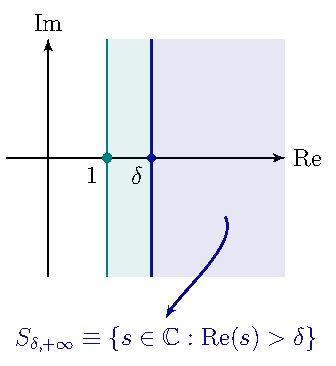
\includegraphics{Figuras/S delta infinito.pdf}
    \end{figure}
    %
    Seja $\delta>1$ e $S_{\delta, +\infty}$  
    o semi-plano dado por
    %
    \[
    S_{\delta, +\infty} 
    \equiv 
    \left\{ s\in\C :\ \Re(s) > \delta \right\}.
    \]
    %
    Para cada $n\in\N$ seja  
    $f_n: S_{\delta, +\infty}\to\C$
    a função holomorfa definida por
    %
    \[
    f_n(s) = \frac{1}{n^s} = \exp(-s\ln n).
    \]
    %
    Note que segue diretamente das definições 
    de $f_n$, $S_{\delta, +\infty}$ e de supremo que
    %
    \[
    \sup_{s\in S_{\delta,+\infty}} |f_n(s)| 
    = 
    \sup_{s\in S_{\delta,+\infty}}
    \exp(-\Re(s)\ln n) 
    \leq 
    \exp(-\delta\ln n).
    \]
    %
    Desta estimativa segue que 
    %
    \[
    \sum_{n=1}^{\infty} 
    \sup_{s\in S_{\delta,+\infty}}|f_n(s)|
    \leq 
    \sum_{n=1}^{\infty} \exp(-\delta\ln n)
    = 
    \sum_{n=1}^{\infty} \frac{1}{n^\delta}
    \]
    %
    e como $\delta > 1$, podemos garantir que 
    a série do lado direito da igualdade acima é convergente.
    Já que cada $f_n$ é holomorfa em $S_{\delta, +\infty}$, segue
    diretamente do Teste-M de Weierstrass que $\zeta$ define de fato uma holomorfa em
    $S_{\delta,+\infty}$. 
    Por fim,
    como $\delta > 1$ foi tomado arbitrariamente, segue que
    $\zeta$ é holomorfa em todo semi-plano $\Re(s) > 1$.
    
    Agora, vamos mostrar que $\zeta$ admite uma extensão meromorfa a $\C$, com apenas
    um polo simples em $s=1$ com resíduo 1. Como veremos, o argumento da extensão de
    $\zeta$ é bem mais delicado que o da extensão da função $\Gamma$. De fato,
    para realizarmos a extensão vamos precisar considerar, além da função $\Gamma$, 
    outra função especial:
    a função teta de Jacobi $\vartheta: \R\to\C$
    dada por
    %
    \begin{equation}
    \index{Função! Teta de Jacobi}
    \label{def-funcao-teta-jacobi}
        \vartheta(t) = \sum_{n=-\infty}^{\infty} e^{-\pi n^2t}.
    \end{equation}
    %
    Assim como $\Gamma$, a função $\vartheta$ também satisfaz uma equação funcional,
    a saber
    %
    \begin{equation}
    \label{eq-funcional-teta}
        \vartheta(t) = t^{-1/2}\vartheta\left( \frac{1}{t} \right), \, \forall t\neq 0.
    \end{equation}
    %
    Também vamos precisar das seguintes estimativas:
    %
    \begin{itemize}
        \item $\vartheta(t) \leq Ct^{-1/2}$, $0 < t \leq 1$;
        \item $|\vartheta(t) - 1| \leq \widetilde{C}e^{-\pi t}$, $t\geq 1$.
    \end{itemize}
    %
    Por comodidade, reunimos estes resultados nos dois lemas a seguir.
    %
    \begin{lema}
    \label{lema-eq-funcional}
        A função $\vartheta$ satisfaz a equação funcional
        %
        \[
        \vartheta(t) = t^{-1/2}\vartheta\left( \frac{1}{t} \right), \, \forall t\neq 0.
        \]
        %
    \end{lema}
    %
    \begin{proof}
        Para mostrar a validade da equação, vamos utilizar a transformada
        de Fourier de $f(x) = e^{-\pi x^2}$ e a Fórmula da Soma de Poisson 
        (Teorema \ref{teo-form-soma-poisson}). Como vimos em
        \eqref{eq-trans-fourier-gaussiana},
        %
        \[
        \widehat{f}(\xi) = \int_{-\infty}^{\infty} e^{-\pi x^2}e^{-2\pi ix\xi} \, d\xi 
                         = e^{-\pi \xi^2}.
        \]
        %
        Portanto, para cada $t>0$ fixado, podemos 
        obter a transformada de Fourier de $g(x) = e^{-\pi tx^2}$, 
        como segue
        %
        \begin{align*}
            \widehat{g}(\xi) &= 
            \int_{-\infty}^{\infty} e^{-\pi tx^2}e^{-2\pi ix\xi} \, dx 
            \\[0.3cm]
             &= \int_{-\infty}^{\infty} 
             e^{-\pi u^2}e^{-2\pi i\frac{u}{\sqrt{t}}\xi} \frac{1}{\sqrt{t}} \, du \\[0.3cm]
             &= \frac{1}{\sqrt{t}}
             \int_{-\infty}^{\infty} e^{-\pi u^2}e^{-2\pi iu\frac{\xi}{\sqrt{t}}} \, du \\[0.3cm]
             &= \frac{1}{\sqrt{t}}\exp\left( -\pi \frac{\xi^2}{t} \right),
        \end{align*}
        %
        onde na segunda igualdade acima usamos a mudança de variáveis
        $u = \sqrt{t}x$. 
        Agora, aplicando a Fórmula da Soma de Poisson obtemos
        %
        \begin{align*}
            \vartheta(t) = \sum_{n\in\Z} e^{-\pi tn^2}
                         = \sum_{n\in\Z} g(n) 
                         = \sum_{n\in\Z} \widehat{g}(n) 
                         = \frac{1}{\sqrt{t}}\sum_{n\in\Z} e^{-\pi n^2/t}
                         = \frac{1}{\sqrt{t}}\vartheta\left( \frac{1}{t} \right).
        \end{align*}
        %
    \end{proof}
    %
    \begin{lema}
    \label{lema-estimativas}
        A função $\vartheta$ satisfaz as estimativas
        %
        \begin{itemize}
            \item $\vartheta(t) \leq Ct^{-1/2}$, $0 < t \leq 1$;
            \item $|\vartheta(t) - 1| \leq \widetilde{C}e^{-\pi t}$, $t\geq 1$.
        \end{itemize}
        %
    \end{lema}
    %
    \begin{proof}
        Começamos com a primeira estimativa. Pela equação funcional \eqref{eq-funcional-teta},
        temos
        %
        \begin{align*}
            |\vartheta(t)| &= \frac{1}{\sqrt{t}}\left| \vartheta\left( \frac{1}{t} \right) \right| \\
                           &= \frac{1}{\sqrt{t}}\left| \sum_{n\in\Z} e^{-\pi n^2/t} \right| \\
                           &= \frac{1}{\sqrt{t}}\left| 1 + 2\sum_{n=1}^{\infty} e^{-\pi n^2/t} \right| \\
                           &\leq \frac{1}{\sqrt{t}}\left( 1 + 2\sum_{n=1}^{\infty} e^{-\pi n^2} \right) \\
                           &= Ct^{-1/2},
        \end{align*}
        %
        onde usamos que $e^{-\pi n^2/t} \leq e^{-\pi n^2}$ para $0 < t \leq 1$ e tomamos
        $C \equiv 1 + 2\sum_{n=1}^{\infty} e^{-\pi n^2}$.
        
        Para o segundo item, basta observar que
        %
        \begin{align*}
            |\vartheta(t) - 1| &= \left| \sum_{n\in\Z} e^{-\pi n^2t} - 1 \right| \\
                               &= \left| 1 + 2\sum_{n=1}^{\infty} e^{-\pi n^2t} - 1 \right| \\
                               &= 2\sum_{n=1}^{\infty} e^{-\pi n^2t} \\
                               &\leq 2\sum_{n=1}^{\infty} e^{-\pi nt} \\
                               &= 2\cdot\frac{e^{-\pi t}}{1 - e^{-\pi t}} \\
                               &\leq \left( \frac{2}{1 - e^{-\pi}} \right)e^{-\pi t} \\
                               &= \widetilde{C}e^{-\pi t}.
        \end{align*}
        %
    \end{proof}
    %
    Tendo estabelecido esses lemas, podemos começar a analisar as relações entre as funções
    $\Gamma$, $\zeta$ e $\vartheta$. 
    Um dos resultados mais importantes envolvendo a relação entre estas
    três funções é o Teorema \ref{teo-zeta-gamma-teta} abaixo. Antes de
    apresentar a prova deste teorema vamos precisar um lema auxiliar. 
    
    \begin{lema}
    \label{lema-aux-teo-zeta-gamma-teta}
    Para todo $s\in \C$ tal que $\Re(s)>1$, vale a identidade mostrada abaixo. 
    Além do mais, as séries e integrais que aparecem nesta expressão são todas convergentes.
    \begin{equation}
        \label{eq-aux1-lema-int-sum-teta}
        \sum_{n=1}^{\infty}\int_0^{\infty} e^{-\pi n^2u}u^{s/2 - 1} \, du
        =
        \int_0^{\infty}\sum_{n=1}^{\infty} e^{-\pi n^2u}u^{s/2 - 1} \, du
    \end{equation}
    \end{lema}
    \begin{proof}
        Vamos começar mostrando que a série que aparece no lado 
        esquerdo de \eqref{eq-aux1-lema-int-sum-teta} é absolutamente convergente para todo $s\in \C$ tal que $\Re(s)>1$. 
        
        Para provar esta convergência é necessário 
        obter uma expressão mais simples que 
        permita entender o comportamento assintótico da $n$-ésima parcela 
        desta soma quando $n\to\infty$. 
        Isto pode ser feito usando o Teorema da Mudança de Variáveis,
        fazendo $\pi n^2 u = t$, e a definição da função Gama
        como segue:
        %
        \begin{align}
        \label{eq-aux2-lema-int-sum-teta}
            \int_0^{\infty} e^{-\pi n^2u}u^{s/2 - 1} \, du 
            &= \int_0^{\infty} e^{-t}t^{s/2 - 1} \left( \frac{1}{\pi n^2} \right)^{s/2} \, dt 
            \nonumber\\[0.3cm]
            &= \pi^{-s/2}\frac{1}{n^s}\int_0^{\infty} e^{-t}t^{s/2 - 1} \, dt 
            \nonumber\\[0.3cm]
            &= \pi^{-s/2}\Gamma\left( \frac{s}{2} \right)\frac{1}{n^s}.
        \end{align}
        %
        Já que o lado direito da expressão acima é absolutamente somável, 
        quando $\Re(s)>1$, podemos concluir que a série que 
        aparece no lado esquerdo 
        de \eqref{eq-aux1-lema-int-sum-teta} é convergente.
        
        
        Sobre o lado direito da igualdade \eqref{eq-aux1-lema-int-sum-teta},
        primeiro observamos que a série que aparece nesta expressão,
        isto é, 
        \[
        \sum_{n=1}^{\infty} e^{-\pi n^2u}
        \]
        é convergente para todo $u>0$, 
        por uma aplicação direta do teste da raiz $n$-ésima. 
        Note que esta série não converge para $u=0$.
        
        Além do mais, segue do teste M de Weierstrass que para cada $s$ fixado a aplicação 
        \[
        u\longmapsto \sum_{n=1}^{\infty} e^{-\pi n^2u} u^{s/2-1}  
        \]
        é holomorfa no semiplano $\{u\in \C: \Re(u)>\delta\}$ para 
        todo $\delta>0$. Consequentemente, como $\delta>0$ é arbitrário segue que a aplicação acima define uma função complexa contínua em $(0,+\infty)$ e portanto Riemann integrável em cada um dos intervalos limitados e fechados desta semi-reta.
        
        O próximo passo na prova do lema é mostrar que para cada $s\in \C$ com $\Re(s)>1$ fixado,
        temos
        \[
        \lim_{N\to\infty}
        \int_0^{\infty}\sum_{n=N}^{\infty} e^{-\pi n^2u}u^{s/2 - 1} \, du
        =
        0.
        \]
        
        Para isto é suficiente mostrar que 
        \[
        \lim_{N\to\infty}
        \int_0^{\infty}\sum_{n=N}^{\infty} |e^{-\pi n^2u}u^{s/2 - 1}| \, du
        =
        0.
        \]
        Note que usando as mesmas cotas da prova do Teste da Integral (veja \eqref{eq-aux1-teste-integral}) temos para todo $u>0$ e $N>1$ a seguinte desigualdade:
        \begin{align}
        \label{eq-aux1-lema-int-soma-theta}
            \sum_{n=N}^{\infty} 
            |e^{-\pi n^2u}u^{s/2 - 1}|
            &=
            u^{\Re(s)/2 - 1} 
            \sum_{n=N}^{\infty} e^{-\pi n^2u}
            \nonumber\\[0.3cm]
            &\leqslant
            u^{\Re(s)/2 - 1}\
            \int_{N}^{\infty} 
            e^{-\pi u x^2}\, dx.
        \end{align}
        
        Usando coordenadas polares e o Teorema de Fubini (como no cálculo clássico da integral Gaussiana) podemos estimar a integral que aparece no lado direito da desigualdade acima. De fato, 
        \begin{align}
        \label{eq-aux2-lema-int-soma-theta}
        \left(
        \int_{N}^{\infty} e^{-\pi u x^2}\, dx
        \right)^2
        &=
        \int_{N}^{\infty}\int_{N}^{\infty}
        e^{-\pi u (x^2+y^2)}\, dx\,dy
        \nonumber\\[0.3cm]
        &=
        \iint_{[N,\infty)\times [N,\infty)}
        e^{-\pi u (x^2+y^2)}\, dx\,dy
        \nonumber\\[0.3cm]
        &\leqslant 
        \int_{0}^{\frac{\pi}{2}}
        \int_{N}^{\infty}
        e^{-\pi u r^2}\, r\,dr\,d\theta
        \nonumber\\[0.3cm]
        &=
        \frac{\pi}{2}\cdot\frac{1}{2\pi u} 
        e^{-\pi u N}
        \leqslant
        \frac{1}{u}e^{-\pi u N}.
        \end{align}
    %
    \begin{figure}[H]\centering
        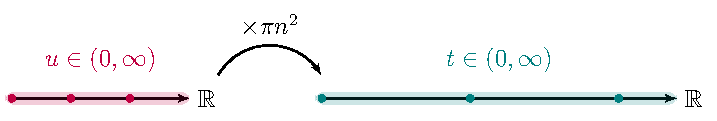
\includegraphics{Figuras/mudança de variável.pdf}
    \end{figure}
    %    
    Tomando a raiz quadrada nos dois lados da desigualdade acima e, em seguida, substituindo a cota obtida em \eqref{eq-aux1-lema-int-soma-theta} 
    ficamos com 
    \begin{align}
    \label{eq-aux3-lema-int-soma-theta}
    \sum_{n=N}^{\infty} 
    |e^{-\pi n^2u}u^{s/2 - 1}|
    \leqslant
    u^{\Re(s)/2 - 1}
    \, u^{-1/2}\, 
    e^{-\frac{\pi u N}{2}}
    =
    u^{\frac{1}{2}(\Re(s)-3)}
    e^{-\frac{\pi u N}{2}}.
    \end{align}

    Portanto, temos 
    \begin{align}
    \int_0^{\infty}\!\sum_{n=N}^{\infty} |e^{-\pi n^2u}u^{s/2 - 1}| \, du
    &\leqslant
    \int_0^{\infty}
    u^{\frac{1}{2}(\Re(s)-3)}
    e^{-\frac{\pi u N}{2}}
    \, du.
    \end{align}
    Usando a mudança de variáveis $t=\pi u N/2$ na integral que aparece no lado direito da desigualdade acima e também que $\Re(s)>1$, obtemos
    \begin{align*}
    \int_0^{\infty}\!\sum_{n=N}^{\infty} |e^{-\pi n^2u}u^{s/2 - 1}| \, du
    &\leqslant
    \frac{2}{\pi N}
    \left(\frac{2}{\pi N}\right)^{\frac{1}{2}(\Re(s)-3)}
    \int_0^{\infty}
    t^{\frac{1}{2}(\Re(s)-3)}
    e^{-t}
    \, dt
    \\[0.3cm]
    &=
    \left(\frac{2}{\pi N}\right)^{\frac{1}{2}(\Re(s)-1)}
    \int_0^{\infty}
    t^{\frac{1}{2}(\Re(s)-1)-1}
    e^{-t}
    \, dt
    \\[0.3cm]
    &=
    \left(\frac{2}{\pi N}\right)^{\frac{1}{2}(\Re(s)-1)}
    \Gamma\left(\frac{1}{2}\left(\Re(s)-1\right)\right).
    \end{align*}
    Como $\Re(s) > 1$, a desigualdade acima permite concluir que 
    \begin{align}
    \label{eq-aux4-lema-int-soma-theta}
    \lim_{N\to\infty}
    \int_0^{\infty}\sum_{n=N}^{\infty} e^{-\pi n^2u}u^{s/2 - 1} \, du
    =
    0.
    \end{align}
    
    Para finalizar, observe que temos das propriedades elementares
    de séries convergentes e da integral de Riemann 
    a seguinte igualdade
    \begin{align*}
    \int_0^{\infty}\sum_{n=1}^{\infty} e^{-\pi n^2u}u^{s/2 - 1} \, du  
    &=
    \int_0^{\infty}
    \left[ 
    \sum_{n=1}^{N-1} e^{-\pi n^2u}u^{s/2 - 1}
    +
    \sum_{n=N}^{\infty} e^{-\pi n^2u}u^{s/2 - 1} 
    \right]
    du
    \\[0.3cm]
    &=
    \sum_{n=1}^{N-1}
    \int_0^{\infty}
    e^{-\pi n^2u}u^{s/2 - 1}\, du
    +
    \int_{0}^{\infty}
    \sum_{n=N}^{\infty} e^{-\pi n^2u}u^{s/2 - 1}\, du.
    \end{align*}
    Tomando o limite quando $N\to\infty$ 
    em ambos lados da igualdade acima e 
    usando \eqref{eq-aux4-lema-int-soma-theta} finalizamos a prova do lema.
    \end{proof}
    %
    \begin{teorema}
    \label{teo-zeta-gamma-teta}
        Para todo $s\in\C$ com $\Re(s) > 1$, vale
        %
        \[
        \pi^{-s/2}\Gamma\left( \frac{s}{2} \right)\zeta(s) 
        = \frac{1}{2}\int_0^{\infty} u^{s/2 - 1}[\vartheta(u) - 1] \, du.
        \]
        %
    \end{teorema}
    %
    \begin{proof}
    A parte mais complicada da prova deste teorema já foi discutida no lema anterior e assim vamos precisar apenas juntar as peças.    
    
    De acordo com \eqref{eq-aux2-lema-int-sum-teta} 
    sabemos que para todo $\Re(s)>1$, 
    vale a seguinte igualdade %
        \[
            \int_0^{\infty} e^{-\pi n^2u}u^{s/2 - 1} \, du
            = \pi^{-s/2}\Gamma\left( \frac{s}{2} \right)\frac{1}{n^s}.
        \]
        %
        Somando, sobre $n\in\N$, ambos lados da identidade acima temos
        %
        \[
            \sum_{n\in\N} \int_0^{\infty} e^{-\pi n^2u}u^{s/2 - 1} \, du
            = 
            \displaystyle\pi^{-s/2}\Gamma\left( \frac{s}{2} \right)\sum_{n\in\N}\frac{1}{n^s} 
        \]
        Como estamos assumindo que $\Re(s)>1$ 
        podemos aplicar o Lema \ref{lema-aux-teo-zeta-gamma-teta}
        para permutar a ordem das soma e da integral
        que aparecem na igualdade acima, ficando com 
        \[
            \int_0^{\infty}
            \sum_{n\in\N} 
            e^{-\pi n^2u}u^{s/2 - 1} \, du
            = 
            \displaystyle\pi^{-s/2}\Gamma\left( \frac{s}{2} \right)\sum_{n\in\N}\frac{1}{n^s} 
        \]
Usando a definição da função $\vartheta$, segue da igualdade acima que 
%
        \[
        \int_0^{\infty} \frac{1}{2}[\vartheta(u) - 1] u^{s/2 - 1} \, du
        = 
        \displaystyle
        \pi^{-s/2}\Gamma\left( \frac{s}{2} \right)\zeta(s)
        \]
o que encerra a prova do teorema.
    \end{proof}
    
    \bigskip 
    
    
    %
    Esse último teorema merece alguns comentários. 
    Observe, primeiramente, que o lado esquerdo
    da identidade contém: 
    \begin{itemize}
        \item uma função inteira, $\pi^{s/2}$;
        
    \item uma função meromorfa em $\C$ com
    polos simples nos inteiros pares não positivos, $\Gamma(s/2)$;
    
    \item e uma função holomorfa em $\Re(s) > 1$.
    
    \end{itemize}
    
    Portanto a aplicação que leva 
    $s\longmapsto \xi(s)$ dada por
    %
    \begin{align}
    \label{def-fun-xi}
    \xi(s) = \pi^{-s/2}\Gamma\left( \frac{s}{2} \right)\zeta(s),
    \end{align}
    %
    define uma função holomorfa no semi-plano $\Re(s) > 1$.
    %
    \begin{teorema}
    \label{teo-form-reflexao-xi}
        A função $\xi$ definida em \eqref{def-fun-xi}
        admite uma continuação analítica à todo domínio $\C\setminus\{0,1\}$,
        que abuso de notação será também denotada por, 
        \[\xi:\C\setminus\{0,1\}\to\C.\]
        As suas singularidades em $s=0$ e $s=1$
        são polos simples e seus resíduos são dados por $\mathrm{res}(\xi,0)=-1$ e $\mathrm{res}(\xi,1)=1$.
        Ademais, ela satisfaz
        a seguinte equação funcional
        %
        \[
        \xi(s) = \xi(1-s), \, \forall s\in\C\setminus\{0,1\}.
        \]
        %
    \end{teorema}
    %
    \begin{proof}
        Por comodidade, consideramos a função auxiliar $\psi:\R_+\to\C$ dada por
        %
        \[
        \psi(u) = \frac{1}{2}[\vartheta(u) - 1].
        \]
        %
        A partir da equação funcional de $\vartheta$, deduzimos a seguinte equação funcional
        para $\psi$:
        %
        \begin{align*}
            \psi(u) &= \frac{1}{2}\left[\frac{1}{\sqrt{u}}\vartheta\left( \frac{1}{u} \right) - 1\right] \\
                    &= \frac{1}{2}\left[\frac{1}{\sqrt{u}}
                    \left( \vartheta\left( \frac{1}{u} \right) - 1 + 1 \right) - 1\right] \\
                    &= \frac{1}{2}\left[\frac{1}{\sqrt{u}}
                    \left( 2\psi\left( \frac{1}{u} \right) + 1 \right) - 1\right] \\
                    &= \frac{1}{\sqrt{u}}\psi\left( \frac{1}{u} \right) + \frac{1}{2\sqrt{u}} - \frac{1}{2}.
        \end{align*}
        %
        Agora, do Teorema \ref{teo-zeta-gamma-teta}, sabemos que
        %
        \begin{align*}
            \pi^{-s/2}\Gamma\left( \frac{s}{2} \right)\zeta(s) 
            = \int_0^{\infty} u^{s/2 - 1}\frac{1}{2}[\vartheta(u) - 1] \, du
            = \int_0^{\infty} u^{s/2 - 1}\psi(u) \, du.
        \end{align*}
        %
        Para calcular esta última integral, vamos dividi-la em duas parcelas e controlar
        cada uma delas:
        %
        \begin{align}
        \label{eq-aux1-teo-eq-func-zeta-completa}
        \int_0^{\infty} u^{s/2 - 1}\psi(u) \, du
        = \int_0^1 u^{s/2 - 1}\psi(u) \, du + \int_1^{\infty} u^{s/2 - 1}\psi(u) \, du.
        \end{align}
        
        %
        Para avaliar a primeira parcela do lado direito, usamos a equação funcional de $\psi$, o Teorema Fundamental do Cálculo e por último uma mudança de variáveis como segue:
        %
        \begin{align*}
            \int_0^1 u^{s/2 - 1}\psi(u) \, du 
            &= 
            \int_0^1 u^{s/2 - 1}
            \left[
                \frac{1}{\sqrt{u}}\psi\left(\frac{1}{u}\right) 
                + \frac{1}{2\sqrt{u}} - \frac{1}{2}
            \right] \, du 
            \\[0.3cm]
            &= 
            \int_0^1
            \left[
                u^{s/2 - 1}u^{-1/2}\psi\left(\frac{1}{u}\right) 
                + \frac{u^{s/2 - 3/2}}{2} - \frac{u^{s/2 - 1}}{2}
            \right] \, du
            \\[0.3cm]
            &= 
            \frac{u^{s/2 - 1/2}}{s-1}\Bigg|_0^1 - \frac{u^{s/2}}{s}\Bigg|_0^1 
            + \int_0^1 u^{s/2 - 1}u^{-1/2}\psi\left(\frac{1}{u}\right) \, du 
            \\[0.3cm]
            &= \frac{1}{s-1} - \frac{1}{s} + \int_0^1 u^{s/2 - 3/2}\psi\left(\frac{1}{u}\right) \, du 
            \\[0.3cm]
            &= \frac{1}{s-1} - \frac{1}{s} + \int_1^{\infty} v^{-s/2 - 1/2}\psi(v) \, dv.
        \end{align*}
        %
        Agora usamos esta expressão em 
        \eqref{eq-aux1-teo-eq-func-zeta-completa} e somamos as duas integrais de forma a obter a seguinte igualdade
        %
        \begin{align*}
            \int_0^{\infty} u^{s/2 - 1}\psi(u) \, du
            = \frac{1}{s-1} - \frac{1}{s} + 
            \int_1^{\infty} \left[u^{-s/2 - 1/2} + u^{s/2 - 1}\right]\psi(u) \, du.
        \end{align*}
        %
        Agora, vamos mostrar que a integral no lado direito define uma função holomorfa da variável complexa $s$.
        Para tanto, defina
        %
        \[
        g_n(s) = \int_1^n \left[ u^{s/2 - 1} + u^{-s/2 - 1/2} \right] \psi(u) \, du.
        \]
        %
        Já que o integrando acima define uma função contínua em $\C\times [1,n]$ podemos usar o Teorema de Fubini para integrar $g_n$ ao longo de  
        qualquer curva de Jordan suave por partes  
        $\y$ contida no plano complexo e desta forma concluir que
        %
        \begin{align*}
            \int_{\y} g_n(s) \, ds 
            &=\int_{\y} \left( 
            \int_1^n \left[ u^{s/2 - 1} + u^{-s/2 - 1/2} \right] \psi(u) \, du \right) \, ds 
            \\[0.3cm]
            &= \int_1^n \psi(u) \int_{\y} \left[ u^{s/2 - 1} + u^{-s/2 - 1/2} \right] \, ds \, du 
            \\[0.3cm]
            &= 0.
        \end{align*}
        %
        Vamos considerar agora a restrição de $g_n$ à faixa
        %
        \[
        S_{-M, M} = \{ s\in\C : -M \leq \Re(s)\leq M \}
        \]
        %
        e mostrar que estas restrições 
        convergem uniformemente para $
        g:S_{-M, M}\to\C$ dada por
        %
        \[
        g(s) 
        = 
        \int_1^{\infty} 
        \left[ 
        u^{s/2 - 1} + u^{-s/2 - 1/2} 
        \right] 
        \psi(u) \, du.
        \]
        
        
        %
        Já sabemos que $g$ está bem definida em $\Re(s) > 1$. Usando o Lema \ref{lema-conv-abs-cond-int-imp}
        sabemos que para mostrar que $g$ está bem
        definida em toda a faixa $S_{-M, M}$, basta mostrar que
        %
        \[
        \int_1^{\infty} \left| u^{s/2 - 1} + u^{-s/2 - 1/2} \right|\cdot|\psi(u)| \, du < +\infty,
        \qquad \forall s\in S_{-M, M}.
        \]
        %
        De fato, para $u\geq 1$ temos que
        %
        \[
        |u^{s/2 - 1} + u^{-s/2 - 1/2}| \leq 2u^{|\Re(s)|/2 - 1/2} \leq 2u^{M/2 - 1/2} \leq 2u^K,
        \]
        %
        sendo $K = M/2 - 1/2$. 
        Do Lema \ref{lema-estimativas}
        e da definição de $\psi$ temos a seguinte 
        equivalência para algumas constantes positivas
        $C_1$ e $C_2$
        %
        \[
        |\vartheta(u) - 1| 
        \leq 
        C_1\, e^{-\pi u} 
        \qquad\iff\qquad 
        |\psi(u)| 
        \leq 
        C_2\, e^{-\pi u},
        \qquad \forall u\geqslant 1.
        \]
        %
        Usando estas três últimas desigualdades e uma comparação básica entre exponenciais e polinômios 
        concluímos que
        %
        \begin{align*}
        \int_1^{\infty} 
        \left| u^{s/2 - 1} + u^{-s/2 - 1/2} \right|\cdot|\psi(u)| 
        \, du
        &\leqslant
        \int_1^{\infty} 2u^{K}\cdot C_2\, e^{\pi u} \, du
        \\
        &\leq 
        \int_1^{\infty} \left( 2u^K\ C_2\ 
        e^{-\pi u/2} \right)e^{-\pi u/2}\, du 
        \\
        &\leq 
        C_3\int_1^{\infty} e^{-\pi u/2} \, du \\
        &< +\infty.
        \end{align*}
        %
        Usando estimativas idênticas às acima, 
        podemos verificar que 
        %
        \begin{align*}
            \sup_{s\in S_{-M,M}} |g_n(s) - g(s)| 
            &\leq 
            \sup_{s\in S_{-M,M}}
            \int_n^{\infty} \left| u^{s/2 - 1} + u^{-s/2 - 1/2} \right|\cdot|\psi(u)| \, du 
            \\[0.3cm]
            &\leq 
            K_1\int_n^{\infty} e^{-\pi u/2} \, du 
            \\
            &= 
            K_2\, e^{-\pi n/2} 
            \xrightarrow{\ n\to\infty\ } 0.
        \end{align*}
        %
        Como para cada $n\in\N$ a função $g_n$ é analítica e que $g_n$ converge uniformemente para $g$,
        quando $n\to\infty$, na faixa $S_{-M, M}$, segue que
        $g$ é analítica em $S_{-M, M}$. 
        
        Por fim, como o parâmetro $M$ que determina a largura da faixa $S_{-M,M}$ é arbitrário, segue que a aplicação
        %
        \begin{equation}
        \label{eq-aux1-cont-analitica-xi}
        s 
        \longmapsto 
        \int_1^{\infty} \left[ u^{s/2 - 1} + u^{-s/2 - 1/2} \right] \psi(u) \, du
        \end{equation}
        %
        define uma função inteira.
        
        Considere então a extensão meromorfa de $\xi$ dada pelo lado direito da igualdade
        %
        \[
        \xi(s) = \frac{1}{s-1} - \frac{1}{s} + \int_1^{\infty} [u^{s/2 - 1} + u^{-s/2 - 1/2}]\psi(u) \, du.
        \]
        %
        Notando que a soma das duas primeiras parcelas e o integrando na igualdade acima são invariantes pela aplicação $s\longmapsto 1-s$ podemos verificar  imediatamente que $\xi(s) = \xi(1-s)$. De fato, 
        %
        \begin{align*}
            \xi(1-s) &= \frac{1}{1-s-1} - \frac{1}{1-s} 
            + \int_1^{\infty} [u^{1/2 - s/2 - 1} + u^{-1/2 + s/2 - 1/2}]\psi(u) \, du \\
            &= \frac{1}{s-1} - \frac{1}{s} + \int_1^{\infty} [u^{s/2 - 1} + u^{-s/2 - 1/2}]\psi(u) \, du \\
            &= \xi(s).
        \end{align*}
        %
    \end{proof}
    %
    Com esse teorema, podemos olhar agora para a função $\zeta$.
    %
    \begin{teorema}
    \label{teo-cont-zeta}
        A função $\zeta:\{ s\in\C : \Re(s) > 1 \} \to \C$ admite uma continuação meromorfa a todo $\C$,
        com apenas um polo simples em $s=1$ com resíduo $1$.
    \end{teorema}
    %
    \begin{proof}
        Já sabemos que para todo $s\in\C$ tal que $\Re(s) > 1$ vale
        %
        \[
        \xi(s) = \pi^{-s/2}\Gamma\left(\frac{s}{2}\right)\zeta(s).
        \]
        %
        Também sabemos que, nessa região, $\Gamma(s/2)\neq 0$. Portanto, é lícito escrever
        %
        \[
        \zeta(s) 
        = 
        \pi^{s/2}\frac{1}{\Gamma(s/2)}\xi(s), 
        \qquad \forall s\in\C, \, \Re(s) > 1.
        \]
        %
        Como $1/\Gamma$ é uma função inteira com zeros 
        de multiplicidade 1 nos inteiros pares não positivos,
        podemos afirmar 
        que existe uma função 
        $g:\C\to\C$ holomorfa com $g(0)\neq 0$ tal que
        %
        \[
        \frac{1}{\Gamma(s)} = s\, g(s) 
        \qquad\implies\qquad
        \frac{1}{\Gamma(s/2)} = \frac{s}{2}\cdot g\Big(\frac{s}{2}\Big).
        \]
        %
        Portanto,
        %
        \begin{align*}
            \zeta(s) &= 
            \pi^{s/2}\frac{1}{\Gamma(s/2)}\xi(s)
            \\[0.3cm]
            &=
            \pi^{s/2}\ \frac{s}{2}\ g\Big(\frac{s}{2}\Big)
            \left( \frac{1}{s-1} - \frac{1}{s} + h(s) \right) 
            \\[0.3cm]
            &= \frac{\pi^{s/2}}{2}\left( \frac{s}{s-1} - 1 + s\, h(s) \right)g\Big(\frac{s}{2}\Big),
        \end{align*}
        %
        sendo $h$ a função inteira que aparece em \eqref{eq-aux1-cont-analitica-xi} 
        ao longo 
        da prova do teorema anterior. 
        O lado direito da identidade acima
        é a extensão procurada, 
        haja vista que define uma função holomorfa em $\C\setminus\{1\}$.
        Resta, portanto, mostrar que $s=1$ é 
        polo simples e calcular seu resíduo. Para tanto,
        basta calcular
        %
        \begin{align*}
            \lim_{s\to 1} (s-1)\zeta(s) 
            &= \lim_{s\to 1} \frac{\pi^{s/2}}{2}\Big( s - (s-1) + (s-1)\,s\,h(s) \Big)g\Big(\frac{s}{2}\Big)\\[0.3cm]
            &= \frac{\pi^{1/2}}{2}\lim_{s\to 1} \left[ s\, g\Big(\frac{s}{2}\Big)\right] \\[0.3cm]
            &= \frac{\pi^{1/2}}{2}\lim_{s\to 1} \frac{2}{\Gamma(s/2)} \\[0.3cm]
            &= \frac{\pi^{1/2}}{2}\cdot\frac{2}{\Gamma(1/2)} \\[0.3cm]
            &= \frac{\pi^{1/2}}{2}\cdot\frac{2}{\pi^{1/2}} \\[0.3cm]
            &= 1.
        \end{align*}
        %
    \end{proof}
    %
    A seguir, vamos mostrar uma representação da função $\zeta$
    em termos de um produtório.
    %
    \begin{teorema}[A Fórmula de Produto de Euler]
    \label{teo-form-prod-euler}
    \index{Fórmula!do Produto de Euler}
        Para todo $s\in\C$ tal que $\Re(s) > 1$, temos
        %
        \[
        \prod_{p\in\mathbb{P}} 
        \left(1 - \frac{1}{p^s} \right)
        \zeta(s) 
        =
        1,
        \]
        %
        onde o produtório que aparece acima converge uniformemente nas
        partes compactas do semi-plano $\{Re(s)>1\}$ e é realizado sobre o conjunto de todos os números primos. Consequentemente, 
        se $\Re(s)>1$ temos $\zeta(s)\neq 0$ e 
        também vale a famosa fórmula de produto de Euler 
        \[
        \zeta(s) 
        =
        \prod_{p\in\mathbb{P}} 
        \left(1 - \frac{1}{p^s} \right)^{-1}.
        \]
    \end{teorema}
    %
    \begin{proof}
        Nesta prova, é de importância fundamental o fato de que a
        série de Dirichlet da função zeta de Riemann, ou seja,
        %
        \[
        \sum_{n=1}^{\infty} \frac{1}{n^s}
        \]
        %
        converge {\bf absolutamente} no semi-plano $\Re(s) > 1$.
        
        Para provar o teorema primeiro vamos mostrar, por indução em $n$, uma identidade auxiliar, que envolve certos produtos parciais. Em seguida, argumentamos que é possível 
        tomar o limite destes produtos parciais, quando $n$ tende a infinito e obter a fórmula desejada. 
        
        O primeiro passo da indução, mencionada acima, consiste em observar que para todo $s\in\C$ tal que $\Re(s)>1$ temos
        da propriedades elementares de séries absolutamente convergentes que
        %
        \begin{align}
        \label{eq:tirando-pares-form-prod}
            \frac{1}{2^s}\zeta(s) 
            &= \frac{1}{2^s}\left(
            1 + \frac{1}{2^s} + \frac{1}{2^s} 
            + \frac{1}{3^s} + \frac{1}{4^s}
            + \frac{1}{5^s} + \cdots
            \right)
            \nonumber\\
            &= \frac{1}{2^s} + \frac{1}{4^s} + \frac{1}{6^s}
            + \frac{1}{8^s} + \frac{1}{10^s} + \cdots.
        \end{align}
        %
        Daí, subtraindo \eqref{eq:tirando-pares-form-prod} da expressão
        em série de Dirichlet de $\zeta$, ficamos com
        %
        \begin{equation}
        \label{eq:zeta-sem-pares}
            \left( 1 - \frac{1}{2^s} \right)\zeta(s) 
            = 1 + \frac{1}{3^s} + \frac{1}{5^s} 
            + \frac{1}{7^s} + \frac{1}{9^s} + \cdots.
        \end{equation}
        %
        Antes de prosseguir com o argumento, é importante frisar um
        ponto: a priori, se $A$ é um conjunto infinito enumerável qualquer e $(a_n)_{n\in A}$ é uma coleção arbitrária de números complexos, indexada em $A$, então a soma dos $a_n$'s sobre $A$, isto é,
        %
        \[
        \sum_{n\in A} a_n,
        \]
        %
        pode não estar bem definida. 
        Isto ocorre, por exemplo, quando a família das 
        somas sobre os subconjuntos finitos de $A$, 
        forma um conjunto de números complexos 
        com mais de um ponto de acumulação. 
        Em outras palavras, dependendo da ordem em que realizamos a
        soma podemos construir somas parciais que convergem para 
        distintos limites ou mesmo que nem sequer convergem.
        Este fenômeno é comum quando lidamos, por exemplo, 
        com séries condicionalmente convergentes.
        
    
        Por outro lado, quando lidamos com uma família de números complexos absolutamente somável, então a ordem
        em que realizamos a soma não é relevante e, 
        nesse caso, o símbolo acima está bem definido.
        
        
        Feita esta ressalva, observamos que todas as somas (finitas e infinitas) que aparecem nos argumentos abaixo 
        são somas absolutamente convergentes. 
        O que permite usar, sem ambiguidade, a notação acima.
        
        Antes de voltar ao argumento de indução vamos introduzir mais algumas notações. Dado um número primo $p$ denotamos o conjunto 
        dos múltiplos de $p$ por 
        %
        \[
        p\N \equiv  \{ p, 2p, 3p, \dots \}.
        \]
        %
        E usaremos a notação 
        %
        \[
        \N(2, 3, \dots, p_n) 
        = \{ 2, 3, 4, \dots \} 
        \setminus \bigcup_{p\in\{2, 3, \dots, p_n\}} p\N,
        \]
        %
        onde $p_n$ o $n$-ésimo primo, para denotar o 
        conjunto de todos os números naturais maiores ou iguais a dois
        que não são múltiplos de $2,3,5,7,11,\ldots p_n$. 
        
        Utilizando esta notação observe que podemos reescrever \eqref{eq:zeta-sem-pares} como 
        %
        \[
        \sum_{n\in\N(2)} \frac{1}{n^s}.
        \]
        %
        Procedendo analogamente, temos que
        %
        \[
        \frac{1}{3^s}\left( 1 - \frac{1}{2^s} \right)\zeta(s)
        = \frac{1}{3^s} + \frac{1}{9^s} + \frac{1}{15^s} + \cdots
        \]
        %
        e, portanto,
        %
        \[
        \left(1 - \frac{1}{3^s}\right)\left(1 - \frac{1}{2^s}\right)\zeta(s)
        = 1 + \frac{1}{5^s} + \frac{1}{7^s} + \frac{1}{11^s} + \cdots
        = 1 + \sum_{n\in\N(2,3)} \frac{1}{n^s}.
        \]
        %
        Segue então por indução em $n$ que
        %
        \begin{align*}
            \left(1 - \frac{1}{p_n^s}\right)
            \cdots
            \left(1 - \frac{1}{3^s}\right)
            \left(1 - \frac{1}{2^s}\right)\zeta(s)
            &= 1 + \sum_{n\in\N(2,3, \dots, p_n)} \frac{1}{n^s} 
            \\[0.5cm]
            \big\Downarrow
            \\[0.5cm]
            \left|
            \prod_{j=1}^n \left(1 - \frac{1}{p_j^s}\right)\zeta(s) - 1
            \right|
            = \left|
            \sum_{j\in\N(2,3, \dots, p_n)} \frac{1}{j^s}
            \right|
            &\leq \sum_{j=p_n}^{\infty} \left|\frac{1}{j^s}\right|,
            \,\quad \forall n\geq 1.
        \end{align*}
        %
        Como a cauda da série de Dirichlet 
        de $\zeta$ converge para $0$,
        segue que
        %
        \[
        \left[
        \lim_{n\to\infty} \prod_{j=1}^n \left(1 - \frac{1}{p_j^s}\right)
        \right]\zeta(s)
        = 1
        \qquad \iff \qquad
        \prod_{p\in\mathbb{P}} \left(1 - \frac{1}{p^s}\right)\zeta(s)
        = 1.
        \]
        %
        
        Como consequência da igualdade acima podemos afirmar que $\zeta(s)\neq 0$ no semi-plano
        $\Re(s) > 1$. 
        
        
        Por fim, lembrando que se uma sequência
        de números complexos $(b_n)_{n\in\N}$ 
        é tal que $b_n\to b\neq 0$,
        então temos que $1/b_n \to 1/b$. 
        Desta propriedade elementar de sequências convergentes e da identidade acima podemos concluir finalmente que 
        %
        \[
        \zeta(s) 
        = \prod_{p\in\mathbb{P}} \left(1 - \frac{1}{p^s}\right)^{-1}.
        \]
        %
    \end{proof}
    %
    
    \subsection{Regiões Livres de Zeros da Função Zeta de Riemann}
    
    Agora, vamos analisar as regiões nas quais a função zeta não se anula.
    O último teorema nos garante que no semi-plano $\Re(s)>1$, $\zeta(s) \neq 0$.
    Da equação funcional para $\zeta$, sabemos que os inteiros pares não positivos,
    $\{0, -2, -4, -6, \dots\}$ são todos zeros dessa função, geralmente chamados
    \textbf{zeros triviais} de $\zeta$.
    %
    \begin{figure}[H]\centering
        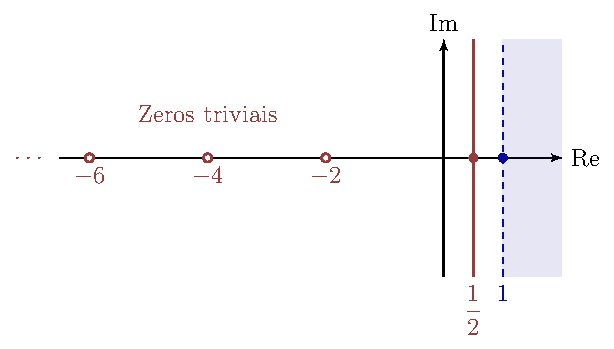
\includegraphics{Figuras/zeros triviais.pdf}
    \end{figure}
    %
    Usando a simetria de $\zeta$ em torno da reta $\Re(s) = 1/2$, vamos argumentar que,
    a menos dos zeros triviais, $\zeta(s)\neq 0$ para todo $s\in\C$ com $\Re(s)<0$.
    
    De fato, como
    %
    \[
    \xi(s) = \pi^{-s/2}\Gamma\left(\frac{s}{2}\right)\zeta(s)
    \]
    %
    para todo $s\in\C$ com $\Re(s)>1$, temos que $\xi$ não se anula nesse semi-plano,
    pois nenhum dos fatores se anula. Daí, segue da equação funcional
    %
    \[
    \xi(s) = \xi(1-s)
    \]
    %
    que $\xi$ também não se anula no semi-plano $\Re(s) < 0$, ou seja, que $\xi(1-s)\neq 0$
    para todo $s\in\C$ com $\Re(s)>1$. Ora, mas
    %
    \[
    \xi(1-s) = \pi^{-(1-s)/2}\Gamma\left(\frac{1-s}{2}\right)\zeta(1-s).
    \]
    %
    Note que $\pi^{-(1-s)/2}\neq 0$ e $\Gamma((1-s)/2)\neq 0$. Portanto, devemos
    necessariamente ter $\zeta(1-s)\neq 0$, ou seja, $\zeta$ não se anula no
    semi-plano $\Re(s) < 0$.
    %
    \begin{figure}[H]\centering
        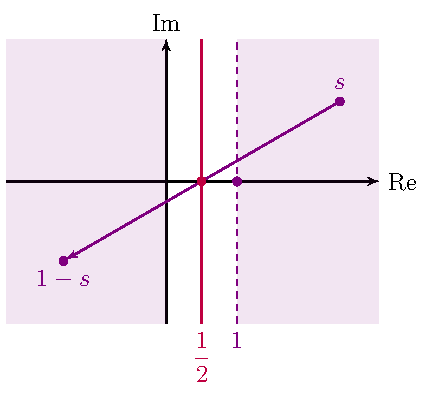
\includegraphics{Figuras/espelho de s.pdf}
    \end{figure}
    %
    \begin{center}
        \red{Falar das quádruplas de zeros}
        
        \red{Falar de $\overline{\zeta(\overline{s})}$}
    \end{center}
    %
    
    
    \subsubsection*{Algumas propriedades adicionais da função Gama}
    %
    Vamos tratar de mais algumas propriedades da função $\Gamma$ que nos
    serão úteis mais à frente, a saber: a ordem de crescimento de $1/\Gamma$
    e sua expressão em termos de uma fórmula de produto. 
    
    Para lidar com a ordem de crescimento de $1/\Gamma$, vamos precisar
    do seguinte lema auxiliar.
    %
    \begin{lema}
    \label{lema-aux-cresc-inv-gama}
        Para todo $s\in\C$ com $1\leq|s|$ e dado $k>0$ fixado qualquer,
        vale a desigualdade
        %
        \[
        e^{k|s|} \leq e^k e^{k|s|\ln|s|}.
        \]
        %
    \end{lema}
    %
    \begin{proof}
        Observe que para mostrar a validade da desigualdade, basta 
        mostrar que
        %
        \[
        e^{k|s|(1 - \ln|s|)} \leq e^k
        \]
        %
        e que mostrar essa última desigualdade, por sua vez, é equivalente a mostrar que
        a função $f$ definida por $f(x) = x(1-\ln x)$ para $x\geq 1$ tem máximo igual a 1.
        Para verificar esse fato, basta observar que
        %
        \[
        f'(x) = 1 - \ln x - x(1/x) = -\ln x \leq 0
        \]
        %
        para todo $x\geq 1$. Portanto, $f$ admite um máximo em $x=1$, que é igual a $1$,
        e fica mostrada a validade do lema.
    \end{proof}
    %
    \begin{teorema}
    \label{teo-ordem-cresc-inv-gama}
        A função $1/\Gamma$ é tal que
        %
        \[
        \left| \frac{1}{\Gamma(s)} \right| \leq K_1e^{K_2|s|\ln|s|}
        \]
        %
        para todo $s\in\C$, sendo $K_1$ e $K_2$ constantes reais positivas,
        ou seja, a ordem de crescimento de $1/\Gamma$ é 1 no sentido de que
        para todo $\e>0$ existe $C(\e)>0$ tal que
        %
        \[
        \left| \frac{1}{\Gamma(s)} \right| \leq C(\e)e^{K_2|s|^{1+\e}},
        \]
        %
        para todo $s\in\C$.
    \end{teorema}
    %
    \begin{proof}
        Nesta demonstração, vamos precisar usar dois fatos importantes obtidos previamente,
        a saber, a equação funcional de $\Gamma$:
        %
        \[
        \Gamma(s)\Gamma(1-s) = \frac{\pi}{\sen(\pi s)}, \, \forall s\in\C\setminus\Z
        \]
        %
        e a extensão de $\Gamma$:
        %
        \[
        \Gamma(s) = \sum_{n=0}^{\infty} \frac{(-1)^n}{n!(n+s)} 
                    + \int_0^{\infty} e^{-t}t^{s-1} \, dt, \, 
                    \forall s\in\C\setminus\{0, -1, -2, \dots\}.
        \]
        %
        Com essas duas identidades, podemos escrever
        %
        \begin{align}
        \label{eq-expressao-inv-gama}
            \frac{1}{\Gamma(s)} &= \Gamma(1-s)\frac{\sen(\pi s)}{\pi} \nonumber \\ 
                                &= \left( \sum_{n=0}^{\infty} \frac{(-1)^n}{n!(n+1-s)} \right)
                                \frac{\sen(\pi s)}{\pi}
                                + \left( \int_0^{\infty} e^{-t}t^{-s} \, dt \right)
                                \frac{\sen(\pi s)}{\pi}, \, \forall s\in\C\setminus\Z.
        \end{align}
        %
        Com isso, dividiremos a prova em duas etapas. Primeiro, vamos estimar a parcela integral
        da identidade acima e, após isso, vamos estimar a parcela em série.
        
        Para a primeira etapa, começamos mostrando que
        %
        \begin{equation}
        \label{eq-cota-int-parte-real}
            \int_1^{\infty} e^{-t} t^{\sigma - 1} \, dt \leq e^{(\sigma + 1)\ln(\sigma + 1)},
        \end{equation}
        %
        sendo $\Re(s) = \sigma \geq 0$. De fato, escolha $n\in\N$ tal que 
        $\sigma \leq n\leq \sigma+1$. Então, usando o fato de que $0< 1/t \leq 1$ e também
        a monotonicidade do logaritmo e da exponencial, temos
        %
        \begin{align*}
            \int_1^{\infty} e^{-t}t^{\sigma - 1} \, dt 
            &\leq \int_1^{\infty} e^{-t}t^{\sigma} \, dt \\
            &\leq \int_1^{\infty} e^{-t} t^n \, dt \\
            &= \Gamma(n+1) \\
            &= n! \\
            &\leq n^n \\
            &= e^{n\ln n} \\
            &\leq e^{(\sigma + 1)\ln(\sigma + 1)}.
        \end{align*}
        %
        Essa desigualdade nos permite concluir que
        %
        \[
        \left| \int_1^{\infty} e^{-t} t^s \, dt \right| \leq e^{(|\sigma|+1)\ln(|\sigma|+1)}, \, 
        \forall s\in\C.
        \]
        %
        Para majorar a segunda parcela de \eqref{eq-expressao-inv-gama}, vamos majorar
        $e^{(|\sigma|+1)\ln(|\sigma|+1)}$. Essa majoração será dividida em duas partes.
        
        Para $0 < |s| < 1$, podemos escrever
        %
        \begin{align*}
            e^{(|\sigma|+1)\ln(|\sigma|+1)} &\leq e^{(|s|+1)\ln(|s|+1)} \\
                                            &= e^{|s|\ln(|s|+1)}e^{\ln(|s|+1)} \\
                                            &\leq 2\exp\left[ |s|\ln\left( |s|(1 + 1/|s|) \right) \right] \\
                                            &\leq 2e^{|s|\ln|s|}e^{|s|\ln(1 + 1/|s|)}.
        \end{align*}
        %
        Observe que, pela Regra de L'Hôpital,
        %
        \begin{align*}
            \lim_{s\to 0} \left[ |s|\ln\left( 1 + \frac{1}{|s|} \right) \right]
            &= \lim_{s\to 0} \frac{\ln(1 + 1/|s|)}{1/|s|} \\
            &= \lim_{x\to 0^+} \frac{\ln(1 + 1/x)}{1/x} \\
            &= \lim_{x\to 0^+} (1 + 1/x)^{-1}(-1/x^2)/(-1/x^2) \\
            &= 0.
        \end{align*}
        %
        Portanto, dado $\e=1$ existe $0<\delta<1$ tal que se $|s|<\delta$ então
        %
        \[
        \left| \frac{\ln(1 + 1/|s|)}{1/|s|} \right| < 1 \implies |\ln(1 + 1/|s|)| \leq 2/|s| 
                                                        \implies |s|\ln(1+1/|s|) \leq 2.
        \]
        %
        Voltando à estimativa, temos que para $0<|s|<1$ vale que
        %
        \begin{align*}
            e^{(|\sigma|+1)\ln(|\sigma|+1)} &\leq 2e^2e^{|s|\ln|s|}.
        \end{align*}
        %
        Agora, para $1\leq|s|$, usamos o Lema \ref{lema-aux-cresc-inv-gama}
        e obtemos
        %
        \begin{align*}
            e^{(|\sigma|+1)\ln(|\sigma|+1)} &\leq e^{(|s|+1)\ln(|s|+1)} \\
                                            &\leq e^{2|s|\ln(2|s|)} \\
                                            &= e^{2|s|(\ln|s| + \ln 2)} \\
                                            &\leq e^{2|s|\ln|s|}e^{2|s|} \\
                                            &\leq e^{2|s|\ln|s|}e^2e^{2|s|\ln|s|} \\
                                            &\leq e^2e^{4|s|\ln|s|}.
        \end{align*}
        %
        Ademais, sabemos que $|\sen(\pi s)| \leq e^{\pi |s|}$ pela Fórmula de Euler. 
        Portanto,
        usando novamente o Lema \ref{lema-aux-cresc-inv-gama},
        a segunda parcela de \eqref{eq-expressao-inv-gama} é majorada por
        %
        \begin{equation}
            \left| \left( \int_0^{\infty} e^{-t}t^{-s} \, dt \right)\frac{\sen(\pi s)}{\pi} \right|
            \leq
            C_1e^{C_2|s|\ln|s|},
        \end{equation}
        %
        sendo
        %
        \[
        C_1 = \begin{cases}
            2e^{\pi + 2}/\pi, \, 0 < |s| < 1 \\
            e^{\pi + 2}/\pi, \, 1\leq |s|
        \end{cases} \qquad \text{ e } \qquad
        C_2 = \begin{cases}
            1, \, 0 < |s| < 1 \\
            4, \, 1\leq |s|
        \end{cases}.
        \]
        %
        
        Agora, precisamos majorar a parcela que envolve a série em \eqref{eq-expressao-inv-gama}.
        Para tanto, vamos dividir nossa análise em dois casos: $|\Im(s)| > 1$ e $|\Im(s)|\leq 1$.
        
        Se $|\Im(s)| > 1$, então $|n+1-s| \geq 1$, como ilustra o diagrama abaixo.
        %
        \begin{figure}[H]\centering
            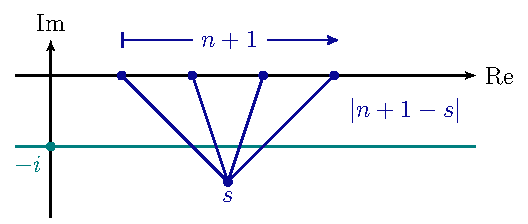
\includegraphics{Figuras/Im(s)>1.pdf}
        \end{figure}
        %
        Daí, segue pela desigualdade triangular que
        %
        \[
        \left| \sum_{n=0}^{\infty} \frac{(-1)^n}{n!(n+1-s)} \right| 
        \leq \sum_{n=0}^{\infty} \frac{1}{n!|n+1-s|} 
        \leq \sum_{n=0}^{\infty} \frac{1}{n!}
        = e.
        \]
        %
        Portanto, como $|\sen(\pi s)| \leq e^{\pi |s|}$ temos que para 
        todo $s\in\C$ com $|\Im(s)|>1$
        vale
        %
        \[
        \left| \left(\sum_{n=0}^{\infty} \frac{(-1)^n}{n!(n+1-s)}\right)\frac{\sen(\pi s)}{\pi} \right|
        \leq \frac{e}{\pi} e^{\pi |s|}
        \leq C_3e^{C_4|s|\ln|s|},
        \]
        %
        sendo $C_3 = e^{\pi + 1}/\pi$ e $C_4 = \pi$ 
        pelo Lema \ref{lema-aux-cresc-inv-gama}.
        
        Agora, se $|\Im(s)| \leq 1$, escolhemos $k\in\Z$ tal que
        %
        \[
        k - \frac{1}{2} \leq \Re(s) < k + \frac{1}{2}.
        \]
        %
        Isso reduz nossa análise a retângulos, como o ilustrado abaixo.
        %
        \begin{figure}[H]\centering
            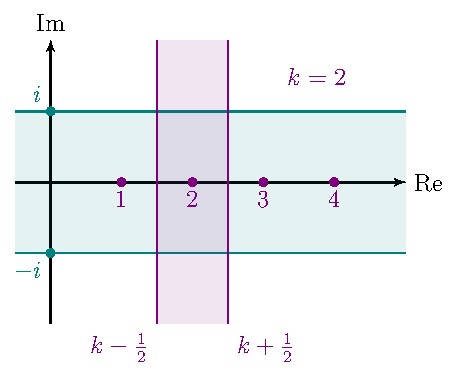
\includegraphics{Figuras/K>=1.pdf}
        \end{figure}
        %
        Para terminar, dividimos a análise novamente em dois sub-casos: $k\geq 1$ e $k\leq 0$.
        
        \paragraph{Caso i): $k\geq 1$.} Nesse caso, podemos escrever
        %
        \begin{align*}
            \left(\sum_{n=0}^{\infty} \frac{(-1)^n}{n!(n+1-s)}\right)\frac{\sen(\pi s)}{\pi}
            = \frac{(-1)^{k-1}\sen(\pi s)}{(k-1)!(k-s)\pi} +
            \left(\sum_{\substack{n\in\N \\ n\neq k}}^{\infty} 
            \frac{(-1)^n}{n!(n+1-s)}\right)\frac{\sen(\pi s)}{\pi}.
        \end{align*}
        %
        Temos que
        %
        \[
        \left|\lim_{s\to k} \frac{\sen(\pi s)}{(k-s)\pi}\right| 
        = \left|\lim_{s\to k} \frac{\pi\cos(\pi s)}{-\pi}\right|
        = 1.
        \]
        %
        Ademais, se $n\neq k$ então $|n+1-s| \geq 1/2$ e, usando o
        Lema \ref{lema-aux-cresc-inv-gama}, temos
        %
        \begin{align*}
            \left|\left(\sum_{\substack{n\in\N \\ n\neq k}}^{\infty} 
            \frac{(-1)^n}{n!(n+1-s)}\right)\frac{\sen(\pi s)}{\pi}\right|
            \leq \frac{2}{\pi}\sum_{\substack{n\in\N \\ n\neq k}} \frac{1}{n!}e^{\pi |s|}
            \leq 2\frac{e}{\pi} e^{\pi |s|}
            \leq C_5e^{C_6 |s|\ln|s|}
        \end{align*}
        %
        sendo $C_5 = 2e^{\pi + 1}/\pi$ e $C_6 = \pi$.
        %
        \paragraph{Caso ii): $k\leq 0$.} Nesse caso, temos $\Re(s) < 1/2$ já que estamos
        supondo que 
        %
        \[
        k - \frac{1}{2} \leq \Re(s) < k + \frac{1}{2}.
        \]
        %
        Portanto,
        %
        \[
        |n+1-s| \geq |n+1 - i\Im(s) - \Re(s)| \geq |n+1 - \Re(s)| \geq \frac{1}{2},
        \]
        %
        conforme ilustra o diagrama abaixo. 
        %
        \begin{figure}[H]\centering
            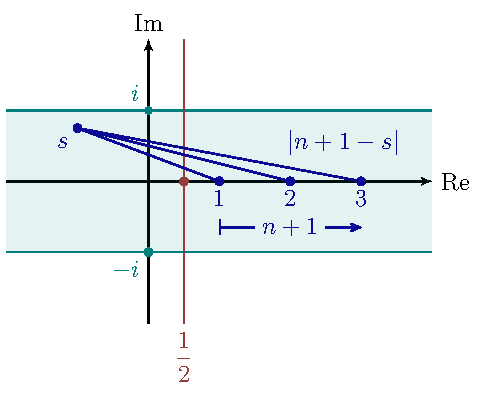
\includegraphics{Figuras/K<=0.pdf}
        \end{figure}
        %
        Logo, novamente usando o Lema \ref{lema-aux-cresc-inv-gama}, temos a estimativa
        %
        \[
        \left|\left(\sum_{n=0}^{\infty} \frac{(-1)^n}{n!(n+1-s)}\right)\frac{\sen(\pi s)}{\pi}\right|
        \leq 2\frac{e}{\pi} e^{\pi |s|} 
        \leq C_7 e^{C_8 |s|\ln|s|}
        \]
        %
        sendo $C_7 = 2e^{\pi + 1}/\pi$ e $C_8 = \pi$ novamente.
        
        Recapitulando, vimos que
        %
        \[
        \left| \left( \int_0^{\infty} e^{-t}t^{-s} \, dt \right)\frac{\sen(\pi s)}{\pi} \right| \leq C_1e^{C_2|s|\ln|s|}
        \]
        %
        sendo
        %
        \[
        C_1 = \begin{cases}
            2e^{\pi + 2}/\pi, \, 0 < |s| < 1 \\
            e^{\pi + 2}/\pi, \, 1\leq |s|
        \end{cases}, \qquad
        C_2 = \begin{cases}
            1, \, 0 < |s| < 1 \\
            4, \, 1\leq |s|
        \end{cases}.
        \]
        %
        e que
        %
        \[
        \left|\left(\sum_{n=0}^{\infty} \frac{(-1)^n}{n!(n+1-s)}\right)\frac{\sen(\pi s)}{\pi}\right| \leq C_3e^{C_4|s|\ln|s|},
        \]
        %
        sendo
        %
        \[
        C_3 = \begin{cases}
            e^{\pi + 1}/\pi, |\Im(s)| > 1 \\
            2e^{\pi + 1}/\pi, |\Im(s)| \leq 1
        \end{cases}, \qquad 
        C_4 = \pi.
        \]
        %
        Portanto, podemos tomar $C_1 = 2e^{\pi + 2}/\pi = C_3$, $C_2 = 4 = C_4$,
        para que as cotas sejam
        válidas para todo $s\in\C$.
        
        Daí, obtemos finalmente
        %
        \begin{align*}
            \left| \frac{1}{\Gamma(s)} \right| 
            &\leq \left|\left(\sum_{n=0}^{\infty} \frac{(-1)^n}{n!(n+1-s)}\right)\frac{\sen(\pi s)}{\pi}\right|
            + \left| \left( \int_1^{\infty} e^{-t} t^{-s} \, dt \right)\frac{\sen(\pi s)}{\pi} \right| \\[0.3cm]
            &\leq C_3e^{C_4|s|\ln|s|} + C_1e^{C_2|s|\ln|s|} \\[0.3cm]
            &= K_1e^{K_2|s|\ln|s|},
        \end{align*}
        %
        sendo
        %
        \[
        K_1 = 2\frac{e^{\pi + 2}}{\pi} \qquad \text{ e } \qquad K_2 = 4.
        \]
        %
    \end{proof}
    %
    
    \medskip
    
    Agora, vamos demonstrar uma belíssima fórmula de produto para $1/\Gamma$.
    %
    \begin{teorema}
    \label{teo-form-prod-inv-gama}
        Para todo $s\in\C$ temos
        %
        \[
        \frac{1}{\Gamma(s)} = e^{\y s}s\prod_{n=1}^{\infty} \left( 1 + \frac{s}{n} \right)e^{-s/n},
        \]
        %
        sendo
        %
        \[
        \y \equiv \lim_{N\to\infty} \sum_{j=1}^N \frac{1}{j} - \ln N
        \]
        %
        a constante de Euler-Mascheroni.
        \index{Constante de Euler-Mascheroni}
    \end{teorema}
    %
    \begin{proof}
        A demonstração é uma aplicação quase direta do Teorema de Hadamard, uma vez que provamos
        no teorema anterior que $1/\Gamma$ tem ordem de crescimento $1$.
        
        Antes, entretanto, vamos mostrar a existência do limite que define $\y$. Para tanto,
        observe que
        %
        \begin{align*}
            \sum_{j=1}^N \frac{1}{j} - \ln N 
            = \sum_{j=1}^N \frac{1}{j} - \int_1^N \frac{1}{x} \, dx
            = \frac{1}{N} + \sum_{j=1}^{N-1} \int_j^{j+1} \left(\frac{1}{j} - \frac{1}{x}\right) \, dx.
        \end{align*}
        %
        Pelo Teorema do Valor Médio aplicado à função $f(y) = 1/y$, sabemos que
        %
        \[
        \left| \frac{1}{j} - \frac{1}{x} \right| \leq \frac{1}{j^2}, \, \forall j\leq x\leq j+1.
        \]
        %
        Portanto,
        %
        \[
        \sum_{j=1}^N \frac{1}{j} - \ln N = \frac{1}{N} + \sum_{j=1}^{N-1} a_j,
        \]
        %
        sendo
        %
        \[
        |a_j| = \left| \int_j^{j+1} \left(\frac{1}{j} - \frac{1}{x}\right) \, dx \right| \leq \frac{1}{j^2}.
        \]
        %
        Logo, sabemos que
        %
        \[
        \sum_{j=1}^{\infty} a_j \leq \sum_{j=1}^{\infty} \frac{1}{j^2} = \frac{\pi^2}{6},
        \]
        %
        de modo que existe
        %
        \[
        \lim_{N\to\infty} \sum_{j=1}^N \frac{1}{j} - \ln N = \sum_{j=1}^{\infty} a_j.
        \]
        %
        
        Feito isto, basta aplicarmos o Teorema de Hadamard a $1/\Gamma$ para obter constantes
        $A,B\in\C$ tais que
        %
        \[
        \frac{1}{\Gamma(s)} = e^{As + B}s\prod_{n=1}^{\infty} \left(1 + \frac{s}{n}\right)e^{-s/n}, \,
        \forall s\in\C.
        \]
        %
        Podemos reescrever essa identidade como
        %
        \[
        1 = e^{As + B}s\Gamma(s)\prod_{n=1}^{\infty} \left(1 + \frac{s}{n}\right)e^{-s/n}.
        \]
        %
        Tomando o limite quando $s\to 0$ e lembrando que $\lim_{s\to 0}s\Gamma(s) = 1$, segue que
        %
        \[
        e^B = 1 \iff B = 0.
        \]
        %
        Por outro lado, tomando $s=1$ na identidade temos
        %
        \begin{align*}
            1 = \frac{1}{\Gamma(1)} &= e^A \prod_{n=1}^{\infty} \left(1 + \frac{1}{n}\right)e^{-1/n} \\
                                &= e^A \lim_{N\to\infty}\prod_{n=1}^{N} \left(1 + \frac{1}{n}\right)e^{-1/n} \\
                                &= e^A \lim_{N\to\infty}\prod_{n=1}^{N} \exp(\ln(1+1/n) - 1/n) \\
                                &= e^A \lim_{N\to\infty} \exp\left[ -\sum_{n=1}^N \frac{1}{n} +
                                                \sum_{n=1}^N \ln(1 + 1/n) \right] \\
                                &= e^A \lim_{N\to\infty} \exp\left[ -\sum_{n=1}^N \frac{1}{n} +
                                                \ln\left( \prod_{n=1}^N (1 + 1/n) \right) \right] \\
                                &= e^A \lim_{N\to\infty} \exp\left[ -\sum_{n=1}^N \frac{1}{n} +
                                                \ln\left( \prod_{n=1}^N \frac{n+1}{n} \right) \right] \\
                                &= e^A \lim_{N\to\infty} \exp\left[ -\sum_{n=1}^N \frac{1}{n} +
                                                \ln(N+1) \right] \\
                                &= e^Ae^{-\y},
        \end{align*}
        %
        onde usamos $\ln(N+1) = \ln(N) + \ln(1 + 1/N)$ e segue que $A = \y + 2\pi ik, k\in\Z$. Ora, mas como $\Gamma(s)\in\R, \, \forall s\in\R$,
        segue que $k = 0$ e $A = \y$, completando a demonstração.
    \end{proof}
    %
    
    \medskip
    
    Agora, vamos voltar a tratar da função $\zeta$. Mostramos
    anteriormente que essa função não se anula fora da faixa
    $0 \leq \Re(s) \leq 1$. Vamos, agora, mostrar que
    $\zeta$ não se anula na reta $\Re(s) = 1$ (isso implicará,
    pela simetria da função, que ela não se anula na reta 
    $\Re(s) = 0$ e, portanto, que todos os zeros não triviais
    da $\zeta$ estão no interior da faixa $0<\Re(s)<1$.
    
    Para provar o resultado, vamos precisar de três lemas
    auxiliares.
    %
    \begin{lema}
    \label{lema-log-zeta}
        Para todo $s\in\C$ tal que $\Re(s)>1$, vale a identidade
        %
        \begin{align}
        \label{eq1-log-zeta}
        \log\zeta(s) 
        = 
        \sum_{p\in \mathbb{P}}\sum_{m=1}^{\infty} \frac{p^{-ms}}{m} 
        = 
        \sum_{n=1}^{\infty} c_nn^{-s},
        \end{align}
        %
        onde $p$ percorre o conjunto dos números primos. Além do mais,
        para cada $n\in\N$ temos $c_n\geq 0$ e cada uma das séries acima convergem absolutamente.
    \end{lema}
    %
    \begin{proof}
        Frisamos, novamente, que a notação $\log\zeta(s)$ \textbf{não} denota a composta entre o ramo principal do logaritmo e a função $\zeta$, mas sim um ramo abstrato do logaritmo de $\zeta$ que é fornecido pela aplicação do Lema \ref{lema-ramo-log}, que realmente pode ser usado neste caso já que $\Re(s)>1$ é um domínio simplesmente conexo onde a função $\zeta$ não se anula.
        
        
        \medskip 
        
        
        Para demonstrar este lema, vamos primeiramente mostrar a validade da identidade \eqref{eq1-log-zeta} quando $s\in\R$ e $s>1$.  
        Em seguida, usaremos um argumento de 
        extensão analítica para verificar que a
        identidade se estende à todo o semi-plano $\Re(s)>1$.
        
        \medskip 
        
        
        Primeiro recordamos que para todo $x\in \R$ tal que $|x|<1$ temos
        %
        \[
        \ln\left( \frac{1}{1-x} \right) = \sum_{m=1}^{\infty} \frac{x^m}{m},
        \]
        %
        com a série acima sendo absolutamente convergente.
        
        Já que $\zeta(s)\in\R_+$ sempre que $s\in\R$ e $s>1$
        podemos usar a representação em produto para $\zeta$ para
        obter a seguinte igualdade%
        \[
        \ln(\zeta(s)) 
        = 
        \ln\left( \prod_{p\in\mathbb{P}} \frac{1}{1 - p^{-s}} \right)
        = 
        \sum_{p\in\mathbb{P}} \ln\left( \frac{1}{1 - p^{-s}} \right)
        = 
        \sum_{p\in \mathbb{P}}\sum_{m=1}^{\infty} \frac{p^{-ms}}{m}.
        \]
        %
        Agora, tomando $c_n = 1/m$ se $n = p^m$ e $c_n = 0$ caso contrário, podemos reescrever
        %
        \[
        \ln(\zeta(s)) = \sum_{n=1}^{\infty} c_n n^{-s}.
        \]
        %
        Até o momento, mostramos que essa expressão é válida para $s\in(1, +\infty)$.
        Ora, mas o lado direito é analítico no semi-plano $\Re(s)>1$, pelo mesmo argumento que 
        usamos para mostrar que $\zeta$ admitia uma representação em série de Dirichlet nesse
        semi-plano. Além disso, sabemos que a função zeta não se anula em $\Re(s)>1$, de modo que
        existe $\log\zeta(s)$ pelo Lema \ref{lema-ramo-log}.
        
        Sabemos que esse ramo do logaritmo para $\zeta$ coincide com o somatório acima no intervalo
        $(1, +\infty)$, que é um conjunto contendo um ponto de aderência, onde estas duas funções coincidem. Portanto, pelo 
        Corolário \ref{cor-unicidade-ext-analiticas}, podemos representar $\log\zeta(s)$
        por
        %
        \[
        \log\zeta(s) = \sum_{n=1}^{\infty} c_n n^{-s},
        \]
        %
        para todo $s\in\C$ com $\Re(s)>1$.
    \end{proof}
    %
    \begin{observacao}
        Na demonstração do lema acima, utilizamos a notação $\prod_{p\in\mathbb{P}}$ para
        o produtório. A rigor, esse símbolo não está bem definido assim como foi o caso
        para os somatórios. Entretanto, como estamos trabalhando com produtos de Weierstrass,
        a Proposição \ref{prop:prod-inf} garante que nessas condições a ordem dos índices
        é irrelevante para o cálculo.
    \end{observacao}
    %
    \begin{lema}
    \label{lema-des-cosseno}
        Para todo $\theta\in\R$, vale a desigualdade
        %
        \[
        3 + 4\cos\theta + \cos 2\theta \geq 0.
        \]
        %
    \end{lema}
    %
    \begin{proof}
        Basta notar que
        %
        \begin{align*}
        0\leqslant 2(1 + \cos\theta)^2  
        &=
        2(1+2\cos\theta+\cos^2\theta)
        \\
        &=
        2\left( 1+2\cos\theta+\frac{1+\cos2\theta}{2} \right)
        \\
        &=
        3 + 4\cos\theta + \cos 2\theta.        
        \end{align*}
        %
    \end{proof}
    %
    O último lema que precisaremos para demonstrar o 
    teorema desejado é consequência dessa desigualdade.
    %
    \begin{lema}
    \label{lema-log-produto-zetas}
        Para todos $\sigma>1$ e $t\in\R$, vale a desigualdade
        %
        \[
        \ln|\zeta^3(\sigma)\zeta^4(\sigma + it)\zeta(\sigma + 2it)|
        \geq 0.
        \]
        %
    \end{lema}
    %
    \begin{proof}
        Seja $s = \sigma + it$. Note que
        %
        \[
        \Re(n^{-s})
        = \Re(e^{-(\sigma + it)\ln n})
        = \Re(e^{-\sigma\ln n}e^{-it\ln n})
        = e^{-\sigma\ln n}\cos(t\ln n)
        = n^{-\sigma}\cos(t\ln n).
        \]
        %
        Usando esse fato e o Lema \ref{lema-log-zeta}, temos
        %
        \begin{align*}
            \ln|\zeta^3(\sigma)\zeta^4(\sigma + it)
            &\zeta(\sigma + 2it)|
            \\[0.3cm]
            &= \ln|\zeta^3(\sigma)| + \ln|\zeta^4(\sigma + it)|
                                    + \ln|\zeta(\sigma + 2it)| \\[0.3cm]
            &= 3\ln|\zeta(\sigma)| + 4\ln|\zeta(\sigma + it)| 
                                   + \ln|\zeta(\sigma + 2it)| \\[0.3cm]
            &= 3\Re(\log(\zeta(\sigma))) + 4\Re(\log(\zeta(\sigma + it)))
                                         + \Re(\log(\zeta(\sigma + 2it))) \\[0.3cm]
            &= \sum_{n=1}^{\infty} c_n \left[\Re(n^{-\sigma}) 
                                        + \Re(n^{-\sigma - it})
                                        + \Re(n^{-\sigma} - 2it) \right] \\[0.3cm]
            &= \sum_{n=1}^{\infty} c_n n^{-\sigma}\left[3 + 4\cos\theta_n
                                                        + \cos 2\theta_n \right],
        \end{align*}
        %
        sendo $\theta_n = t\ln n$ e $c_n\geq 0$ como definidos na prova
        do Lema \ref{lema-log-zeta}. Pelo Lema \ref{lema-des-cosseno}, segue que
        %
        \[
        \sum_{n=1}^{\infty} c_n n^{-\sigma}\left[3 + 4\cos\theta_n
                                                        + \cos 2\theta_n \right]
        \geq 0,
        \]
        %
        e temos o resultado desejado.
    \end{proof}
    %
    
    \medskip
    
    
    Podemos agora enunciar precisamente e demonstrar o teorema desejado.
    %
    \begin{teorema}
    \label{teo-zeta-nao-nula-re1}
        A função $\zeta$ não se anula na reta $\Re(s) = 1$, ou seja,
        $\zeta(1 + it) \neq 0$ para todo $t\in\R$.
    \end{teorema}
    %
    \begin{proof}
        Suponha, por absurdo, que $\zeta(1 + it_0) = 0$ para algum 
        $t_0\in\R^*$. Como $\zeta$ é holomorfa em $1 + it_0$, existe
        uma vizinhança desse ponto tal que
        %
        \[
        \zeta(s) = (s - (1 + it_0))^n g(s),
        \]
        %
        onde $g(s)$ é uma função holomorfa e que não se anula em $1 + it_0$
        na vizinhança. 
        %
        \begin{figure}[H]\centering
            \includegraphics{Figuras/vizinhança.pdf}
        \end{figure}
        %
        Daí, para $2 > \sigma > 1$ temos
        %
        \[
        |\zeta(\sigma + it_0)|^4 = |\sigma-1|^{4n}|g(\sigma + it_0)|^4
                                 \leq C_1(\sigma-1)^4,
        \]
        %
        sendo $C_1 = |g(\sigma + it_0)|^4$. Ademais, como $s=1$ é polo simples
        de $\zeta$, sabemos que
        %
        \[
        |\zeta(\sigma)|^3 = \frac{C_2}{(\sigma - 1)^3},
        \]
        %
        para alguma constante positiva $C_2$. Por último, como $\zeta$ 
        também é holomorfa em $\sigma + 2it_0$, segue que
        $|\zeta(\sigma + 2it_0)|$ é limitado na vizinhança que estamos
        considerando por, digamos, $C_3 > 0$. Portanto,
        %
        \[
        |\zeta(\sigma)^3\zeta^4(\sigma + it_0)\zeta(\sigma + 2it_0)|
        \leq C_1C_2C_3(\sigma - 1) \xrightarrow{\sigma\to 1} 0,
        \]
        %
        ou seja,
        %
        \[
        \ln|\zeta(\sigma)^3\zeta^4(\sigma + it_0)\zeta(\sigma + 2it_0)| 
        \xrightarrow{\sigma\to 1} -\infty,
        \]
        %
        contrariando o Lema \ref{lema-log-produto-zetas}. Portanto,
        $\zeta$ não se anula na reta $\Re(s) = 1$, como afirmado.
    \end{proof}
    %
    
    \medskip
    
    A primeira consequência imediata deste teorema é que $\zeta$ 
    não se anula sobre o eixo imaginário, isto é, sobre a reta $\Re(s) = 0$.
    Portanto, todos os zeros não triviais de $\zeta$ se encontram na
    chamada \textbf{faixa crítica}: $0 < \Re(s) < 1$.
    %
    \begin{figure}[H]\centering
        \includegraphics{Figuras/faixa crítica.pdf}
    \end{figure}
    %
    A famosa \textbf{hipótese de Riemann} afirma que todos os zeros não
    triviais de $\zeta$ se encontram sobre a reta crítica, isto é,
    são da forma $1/2 + it$, com $t\in\R$.
    
    
    \subsection{A função zeta de Riemann e o Teorema do Número Primo}
    
    Nesta seção, vamos utilizar a função $\zeta$ para provar o
    Teorema do Número Primo
    \index{Teorema!do Número Primo}, que diz que
    %
    \[
    \pi(x) \sim x/\log x,
    \]
    %
    sendo $\pi(x)$ a quantidade de números primos menores ou iguais a $x$, e
    onde $\sim$ significa que $\pi(x)$ e $x/\log x$ são assintoticamente equivalentes
    no infinito, isto é, que
    %
    \[
    \lim_{x\to\infty} \frac{\pi(x)}{x/\log x} = 1.
    \]
    %
    Para tanto, vamos precisar de alguns resultados que nos dão informação
    acerca do crescimento de $\zeta$. O primeiro deles é o seguinte.
    %
    \begin{proposicao}
    \label{prop-2.5-Stein}
        Dado $s = \sigma + it$, com $\sigma, t\in\R$, 
        existe uma sequência $\{f_n\}_{n\in\N}$ de funções inteiras
        satisfazendo 
        %
        \[
        |f_n(s)| \leq \frac{|s|}{n^{\sigma + 1}}
        \]
        %
        e tais que, para todo $N\in\N^*$, vale
        %
        \begin{equation}
        \label{eq-8-Stein}
            \sum_{1\leq n < N} \frac{1}{n^s}
            -
            \int_1^N \frac{1}{x^s} \, dx
            =
            \sum_{1\leq n < N} f_n(s).
        \end{equation}
        %
    \end{proposicao}
    %
    \begin{proof}
        Para cada $n\in\N$, defina $f_n:\C\to\C$ por
        %
        \begin{equation}
        \label{eq-def-fn}
            f_n(s) = 
            \int_n^{n+1} \left[ \frac{1}{n^s} - \frac{1}{x^s} \right] \, dx.
        \end{equation}
        %
        Observe que $f_n$ é inteira para cada $n\in\N$. De fato, dado um triângulo 
        $\Delta\subseteq\C$ qualquer, podemos usar o Teorema de Fubini
        e o Teorema de Cauchy-Goursat para concluir que
        %
        \begin{align*}
            \int_{\Delta} f_n(s) \, ds
            &= 
            \int_{\Delta}\left[\int_n^{n+1}\frac{1}{n^s} - \frac{1}{x^s} \, dx\right] \, ds \\
            &= \int_n^{n+1}\left[\int_{\Delta}\frac{1}{n^s} - \frac{1}{x^s} \, ds\right] \, dx \\
            &= \int_n^{n+1} 0 \, dx \\
            &= 0.
        \end{align*}
        %
        Como $\Delta$ era um triângulo qualquer, segue do Teorema de Cauchy-Goursat que
        $f_n$ é inteira para cada $n\in\N$.
        
        {\red Agora, note que aplicando o Teorema do Valor Médio à função $f(x) = x^{-s}$, temos que}
        %
        \[
        \left|\frac{1}{n^s} - \frac{1}{x^s}\right| \leq \frac{|s|}{n^{\sigma + 1}},
        \]
        %
        para todo $n\leq x\leq n+1$. Pelo Lema Técnico (Lema \ref{lema-tecnico}) e por
        \eqref{eq-def-fn}, segue que
        %
        \[
        |f_n(s)| \leq \int_n^{n+1} \left|\frac{1}{n^s} - \frac{1}{x^s}\right| \, dx \leq \frac{|s|}{n^{\sigma + 1}}.
        \]
        %
        Por outro lado, podemos escrever
        %
        \begin{equation}
        \label{eq-int-reescrita}
            \int_1^N \frac{1}{x^s} \, dx = \sum_{1\leq n < N} \int_n^{n+1} \frac{1}{x^s} \, dx.
        \end{equation}
        %
        Logo, juntando \eqref{eq-int-reescrita} com \eqref{eq-def-fn} obtemos
        %
        \begin{align*}
        \sum_{1\leq n < N} \frac{1}{n^s} - \int_1^N \frac{1}{x^s} \, dx
        &= \sum_{1\leq n < N} \left[ \frac{1}{n^s} - \int_n^{n+1} \frac{1}{x^s} \, dx\right] \\
        &= \sum_{1\leq n < N} \int_n^{n+1} \left[ \frac{1}{n^s} - \frac{1}{x^s} \right] \, dx \\
        &= \sum_{1\leq n < N} f_n(s),
        \end{align*}
        %
        como afirmado.
    \end{proof}
    %
    O que nos será mais útil é o seguinte corolário desta proposição.
    %
    \begin{corolario}
    \label{cor-zeta-menos-singularidade}
        Para todo $s\in\C$ com $\Re(s) > 0$, temos
        %
        \[
        \zeta(s) - \frac{1}{s-1} = H(s),
        \]
        %
        onde
        %
        \[
        H(s) = \sum_{n=1}^{\infty} f_n(s)
        \]
        %
        define uma função holomorfa em $\Re(s) > 0$, sendo
        %
        \[
        f_n(s) = \int_n^{n+1} \left[ \frac{1}{n^s} - \frac{1}{x^s} \right] \, dx.
        \]
        %
    \end{corolario}
    %
    \begin{proof}
        Para provar a analiticidade de $H$ no semi-plano $\Re(s) > 0$, vamos usar o
        teste $M$ de Weierstrass.
        
        Seja $\delta > 0$ e suponha que $s$ está no semi-plano $\Re(s) > \delta$. 
        {\red Então, para todo $s$ nesse semi-plano, sabemos que}
        %
        \[
        |f_n(s)| \leq \frac{1}{n^{\delta + 1}},
        \]
        %
        de modo que
        %
        \[
        \sum_{n=1}^{\infty} \sup_{\Re(s) > \delta} |f_n(s)| 
        \leq \sum_{n=1}^{\infty} \frac{1}{n^{\delta + 1}}
        = \zeta(1 + \delta)
        < +\infty.
        \]
        %
        Portanto, pelo teste M de Weierstrass sabemos que $H$ é holomorfa no semi-plano
        $\Re(s) > \delta$. Ora, como $\delta>0$ foi tomado arbitrariamente, então
        $H$ é holomorfa no semi-plano $\Re(s) > 0$.
        
        {\red Agora, observe que para todo $s\in\C$ com $\Re(s) > 1$ podemos escrever}
        %
        \begin{align*}
            \zeta(s) - \frac{1}{s-1} &= \sum_{n=1}^{\infty} \frac{1}{n^s} - \frac{1}{s-1} \\
                                     &= \lim_{N\to\infty} \left(\sum_{n=1}^N \frac{1}{n^s} - \frac{1}{s-1} \right) \\
                                     &= \lim_{N\to\infty} \left(\sum_{n=1}^N \frac{1}{n^s} 
                                                            - \int_1^N \frac{1}{x^s} \, dx \right) \\
                                     &= \lim_{N\to\infty} \sum_{n=1}^N f_n(s) \\
                                     &= H(s)
        \end{align*}
        %
        {\red notando que}
        %
        \[
        \int_1^N x^{-s} \, dx = \frac{N^{-s + 1}}{-s+1} + \frac{1}{s-1}
        \]
        %
        {\red e que a primeira parcela desaparece quando $N\to\infty$.}
        
        {\red checar o argumento e, se estiver certo, argumentar sobre a extensão analítica de $\zeta$}.
    \end{proof}
    %
    \begin{proposicao}
    \label{prop-2.7-Stein}
        Suponha que $s = \sigma + it$, sendo $\sigma, t\in\R$. Então para cada $\sigma_0$ fixado
        com $0\leq\sigma_0\leq1$ e para todo $\e>0$ existe uma uma constante $C_{\e}$ tal que
        %
        \begin{enumerate}[i)]
            \item $|\zeta(s)| \leq C_{\e}|t|^{1-\sigma_0+\e}$ se $\sigma_0\leq\sigma$ e $|t|\geq 1$;
            \item $|\zeta'(s)| \leq C_{\e}|t|^{\e}$ se $1\leq\sigma$ e $|t|\geq 1$.
        \end{enumerate}
        %
    \end{proposicao}
    %
    \begin{observacao}
        Note que essa proposição nos diz que
        %
        \[
        |\zeta(1+it)| \leq C_{\e}|t|^{\e}, 
        \]
        %
        para todo $t\gg 1$.
    \end{observacao}
    %
    \begin{proof}
        Vamos considerar a mesma sequência $\{f_n\}_{n\in\N}$ definida na Proposição \ref{prop-2.5-Stein}, a saber,
        a sequência de funções $f_n:\C\to\C$ definida por
        %
        \[
        f_n(s) = \int_n^{n+1} \left[ \frac{1}{n^s} - \frac{1}{x^s} \right] \, dx.
        \]
        %
        \begin{enumerate}
            \item Observe que, utilizando a desigualdade triangular, propriedades elementares da integral e o fato de que
            $\sigma_0\leq\sigma$, temos
            %
            \begin{align*}
                |f_n(s)| &\leq \int_n^{n+1} \left|\frac{1}{n^s} - \frac{1}{x^s}\right| \, dx \\
                         &\leq \int_n^{n+1} \frac{1}{|n|^s} + \frac{1}{|x|^s} \, dx \\
                         &\leq \int_n^{n+1} \frac{2}{|n|^s} \, dx \\
                         &= \frac{2}{|n^s|} \\
                         &= \frac{2}{n^{\sigma}} \\
                         &\leq \frac{2}{n^{\sigma_0}}.
            \end{align*}
            %
            Dado $\delta \geq 0$ qualquer, podemos usar essa cota e a Proposição \ref{prop-2.5-Stein} para deduzir que
            %
            \[
            |f_n(s)| = |f_n(s)|^{\delta}|f_n(s)|^{1-\delta} 
                     \leq \left(\frac{|s|}{n^{\sigma_0+1}}\right)^{\delta}\left(\frac{2}{n^{\sigma_0}}\right)^{1-\delta}
                     \leq \frac{2|s|^{\delta}}{n^{\sigma_0+\delta}},
            \]
            %
            sendo $0\leq\sigma_0\leq 1$ e $\sigma_0\leq\sigma$. Daí, tomando $\delta = 1 - \sigma_0 + \e$, temos
            %
            \[
            |f_n(s)| \leq \frac{2|s|^{1 - \sigma_0 + \e}}{n^{\sigma_0 + 1 - \sigma_0 + \e}} = \frac{2|s|^{1 - \sigma_0 + \e}}{n^{1 + \e}}.
            \]
            %
            Somando em $n\in\N$ e usando o Corolário \ref{cor-zeta-menos-singularidade}, segue que
            %
            \begin{align*}
                |\zeta(s)| &= \left|\sum_{n=1}^{\infty} f_n(s) + \frac{1}{s-1}\right| \\
                           &\leq \sum_{n=1}^{\infty} |f_n(s)| + \frac{1}{|s-1|} \\
                           &\leq \sum_{n=1}^{\infty} \frac{2|s|^{1 - \sigma_0 + \e}}{n^{1+\e}} + \frac{1}{|s-1|} \\
                           &\leq 2|s|^{1 - \sigma_0 + \e}\zeta(1 + \e) + \frac{1}{|s-1|}.
            \end{align*}
            %
            Aqui vamos dividir nossa análise em dois casos: quando $0 < \sigma \leq 2$ e quando $\sigma > 2$.
            %
            \paragraph{Caso 1: $0 < \sigma \leq 2$.}
            a
            %
            \paragraph{Caso 2: $\sigma > 2$.}
            a
            
        \end{enumerate}
    \end{proof}
    %

\addcontentsline{toc}{part}{%
    \fontfamily{ptm}\selectfont\textit{Módulo 3}
}
\part*{%
    \fontfamily{ptm}\selectfont\textit{Módulo 3}
}

\appendix

\chapter{On the Number of Primes Less Than a Given Magnitude}

%\hfill%
%\begin{minipage}{10cm}
\begin{flushleft}
\rightskip=0.5cm
by BERNHARD RIEMANN\footnote{Translated from \textit{Uber die Anzahl der Primzahlen unter einer gegebenen Grösse} by H.M. Edwards.}
\end{flushleft}
%\end{minipage}

I believe I can best express my gratitude for the honor which the Academy 
has bestowed on me in naming me as one of its correspondents by immediately 
availing myself of the privilege this entails to communicate an investigation
of the frequency of prime numbers, a subject which because of the interest
shown in it by Gauss and Dirichlet over many years seems not wholly unworthy
of such a communication.

In this investigation I take as my starting point the observation of Euler
that the product
%
\[
\prod \frac{1}{1 - \dfrac{1}{p^s}} = \sum \frac{1}{n^s},
\]
%
where $p$ ranges over all prime numbers and $n$ over all whole numbers. The
function of a complex variable $s$ which these two expressions define when they
converge I denote by $\zeta(s)$. They converge only when the real part of $s$
is greater than $1$; however, it is easy yo find and expression of the function
always is valid. By applying the equation
%
\[
\int_0^{\infty} e^{-nx}x^{s-1} \, dx = \frac{\prod(s-1)}{n^s},
\]
%
one finds first
%
\[
\prod(s-1)\zeta(s) = \int_0^{\infty} \frac{x^{s-1}\, dx}{e^x - 1}.
\]
%
If one considers the integral
%
\[
\int \frac{(-x)^{s-1} \, dx}{e^x - 1}
\]
%
from $+\infty$ to $+\infty$ in the positive sense around the boundary
of a domain which contains the value 0 but no other singularity of the
integrand in its interior, then it is easily seen to be equal to
%
\[
(e^{-\pi si} - e^{\pi si})\int_0^{\infty} \frac{x^{s-1} \, dx}{e^x - 1},
\]
%
provided that in the many-valued function $(-x)^{s-1} = e^{(s-1)\log(-x)}$
the logarithm of $-x$ is determined in such a way that it is real for negative
values of $x$. Thus
%
\[
2\sin\pi s\prod(s-1)\zeta(s) 
= i \int_{\infty}^{\infty} \frac{(-x)^{s-1} \, dx}{e^x - 1}
\]
%
when the integral is defined as above.

This equation gives the value of the function $\zeta(s)$ for all complex
$s$ and shows that it is single-valued and finite for all values of $s$
other than 1, and also that it vanishes when $s$ is a negative even integer.

When the real part of $s$ is negative, the integral can be taken, instead
of in the positive sense around the boundary of the given domain, in the
negative sense around the complement of this domain because in that case
(when $\Re s < 0$) the integral over values with infinitely large modulus
is infinitely small. But inside this complementary domain the only singularities
of the integrand are at the integer multiples of $2\pi i$, and the integral 
is therefore equal to the sum of the integrals taken around these singularities
in the negative sense. Since the integral around the value $n2\pi i$ is
$(-n2\pi i)^{s-1}(-2\pi i)$, this gives
%
\[
2\sin\pi s\prod(s-1)\zeta(s) = (2\pi)^s\sum n^{s-1}[(-i)^{s-1} + i^{s-1}],
\]
%
and therefore a relation between $\zeta(s)$ and $\zeta(1-s)$ which, by making
use of known properties of the function $\prod$, can also be formulated as the
statement that
%
\[
\prod\left(\frac{s}{2} - 1\right)\pi^{-s/2}\zeta(s)
\]
%
remains unchanged when $s$ is replaced by $1-s$.

This property of the function motivated me to consider the integral 
$\prod ((s/2) - 1)$ instead of the integral $\prod(s-1)$ in the general
term of $\sum n^{-s}$, which leads to a very convenient expression of
the function $\zeta(s)$. In fact
%
\[
\frac{1}{n^s}\prod\left(\frac{s}{2} - 1\right)\pi^{-s/2}
= \int_0^{\infty} e^{-nn\pi x}x^{(s/2) - 1} \, dx;
\]
%
so when one sets
%
\[
\sum_{1}^{\infty} e^{-nn\pi x} = \psi(x),
\]
%
it follows that
%
\[
\prod\left(\frac{s}{2} - 1\right)\pi^{-s/2}\zeta(s)
= \int_0^{\infty} \psi(x)x^{(s/2) - 1} \, dx
\]
%
or, because
%
\begin{equation*}
\tag{Jacobi, Fund., p. 184}
2\psi(x) + 1 = x^{-1/2}\left[ 2\psi\left(\frac{1}{x}\right) + 1 \right],
\end{equation*}
%
that
%
\begin{align*}
    \prod\left(\frac{s}{2} - 1\right) 
    &= \int_1^{\infty} \psi(x)x^{(s/2) - 1} \, dx
    + \int_0^1 \psi\left(\frac{1}{x}\right) x^{(s-3)/2} \, dx \\
    &+ \frac{1}{2}\int_0^1 (x^{(s-3)/2} - x^{(s/2) - 1}) \, dx \\
    &= \frac{1}{s(s-1)} 
    + \int_1^{\infty} \psi(x)(x^{(s/2) - 1} + x^{-(1+s)/2}) \, dx.
\end{align*}
%
I now set $s = \frac{1}{2} + ti$ and
%
\[
\prod\left(\frac{s}{2}\right)(s-1)\pi^{-s/2}\zeta(s) = \xi(t)
\]
%
so that
%
\[
\xi(t) = \frac{1}{2} - 
\left(tt + \frac{1}{4}\right)\int_1^{\infty} \psi(x)x^{-3/4}
\cos\left(\frac{1}{2}t\log x\right) \, dx
\]
%
or also
%
\[
\xi(t) = 4\int_1^{\infty} \frac{d[x^{3/2}\psi'(x)]}{dx}
x^{-1/4}\cos\left(\frac{1}{2}t\log x\right) \, dx.
\]
%
This function is finite for all finite values of $t$ and can be developed
as a power series in $tt$ which converges very rapidly. Now since for values
of $s$ with real part greater than 1, $\log\zeta(s) = - \sum \log(1 - p^{-s})$
is finite and since the same is true of the other factors of $\xi(t)$, the
function $\xi(t)$ can vanish only when the imaginary part of $t$ lies
between $\frac{1}{2}i$ and $-\frac{1}{2}i$. The number of roots of $\xi(t) = 0$
whose real parts lie between 0 and $T$ is about
%
\[
= \frac{T}{2\pi}\log\frac{T}{2\pi} - \frac{T}{2\pi}
\]
%
because the integral $\int d\log\xi(t)$ taken in the positive sense around the
domain consisting of all values whose imaginary parts lie between $\frac{1}{2}i$
and $-\frac{1}{2}i$ and whose real parts lie between 0 and $T$ is
(up to a fraction of the order of magnitude of $1/T$) equal to
$[T\log(T/2\pi) - T]i$ and is, on the other hand, equal to the number
of roots within these bounds and it is very likely that all of the
roots are real. One would of course like to have a rigorous proof
of this, but I have put aside the search for such a proof after some fleeting
vain attempts because it is not necessary for the immediate objetive of my
investigation.

If one denotes by $\alpha$ the roots of the equation $\xi(\alpha) = 0$,
then one can express $\log\xi(t)$ as
%
\[
\sum\log\left(1 - \frac{tt}{\alpha\alpha}\right) + \log\xi(0)
\]
%
because, since the density of roots of size $t$ grows only like $\log(t/2\pi)$
as $t$ grows, this expression converges and for infinite $t$ is only infinite
like $t\log t$; thus it differs from $\log\xi(t)$ by a function of $tt$ which
is continuous and finite for finite $t$ and which, when divided by $tt$, is
infinitely small for infinite $t$. This difference is therefore a constant, 
the value of which can be determined by setting $t=0$.

With these preparatory facts, the number of primes less than $x$ can now be
determined.

Let $F(x)$, when $x$ is not exactly equal to a prime, be equal to this number,
but when $x$ is a prime let it be greater by $\frac{1}{2}$ so that for an $x$
where $F(x)$ jumps
%
\[
F(x) = \frac{F(x+0) + F(x-0)}{2}.
\]
%
If one sets
%
\[
p^{-s} = s\int_p^{\infty} x^{-s-1} \, dx, 
\qquad
p^{-2s} = s\int_{p^2}^{\infty} x^{-s-2} \, dx,
\qquad
\dots
\]
%
in the formula
%
\[
\log\zeta(s) = -\sum\log(1 - p^{-s}) 
             = \sum p^{-s} + \frac{1}{2}\sum p^{-2s} + \frac{1}{3}\sum p^{-3s}
             + \cdots,
\]
%
one finds
%
\[
\frac{\log\zeta(s)}{s} = \int_1^{\infty} f(x)x^{-s-1} \, dx
\]
%
when one denotes
%
\[
F(x) + \frac{1}{2}F(x^{1/2}) + \frac{1}{3}F(x^{1/3}) + \cdots
\]
%
by $f(x)$.

This equation is valid for every complex value $a+bi$ os $s$ provided $a>1$.
But when in such circumstances
%
\[
g(s) = \int_0^{\infty} h(x)x^{-s} d\log x
\]
%
is valid, the function $h$ can be expressed in terms of $g$ by means of 
Fourier's theorem. The equation splits when $h$ is real and when 
$g(a+bi) = g_1(b) + ig_2(b)$ into the equation
%
\begin{align*}
    g_1(b) &= \int_0^{\infty} h(x)x^{-a}\cos(b\log x) d\log x, \\
    ig_2(b) &= -i\int_0^{\infty} h(x)x^{-a}\sin(b\log x) d\log x.
\end{align*}
%
When both equations are multiplied by $[cos(b\log y) + i\sin(b\log y)]\, db$
and integrated from $-\infty$ to $+\infty$, one finds in both cases that the
right side is $\pi h(y)y^{-\alpha}$ so that when they are added and multiplied
by $iy^{\alpha}$
%
\[
2\pi i h(y) = \int_{a - \infty y}^{a + \infty t} g(s) y^s \, ds,
\]
%
where the integration is to be carried out in such a way that the real part
of $s$ remains constant.

The integral represents, for a value of $y$ where the function $h(y)$ has a
jump, the middle value between the two values of $h$ on either side of the
jump. The function $f$ was defined in such a way that it too has this property,
so one has in full generality
%
\[
f(y) 
= \frac{1}{2\pi i}\int_{a-\infty i}^{a+\infty i} \frac{\log\zeta(s)}{s}y^s \, ds.
\]
%
For $\log\zeta$ when can now substitute the expression
%
\begin{align*}
    \frac{s}{2}\log\pi - \log(s-1) - \log\prod\left(\frac{s}{2}\right) \\
    + \sum_{\alpha} \log\left[1 + \frac{(s - \frac{1}{2})^2}{\alpha\alpha}\right]
    + \log\xi(0)
\end{align*}
%
found above; the integrals of the individual terms of this expression will not
converge, however, when they are taken to infinity, so it is advantageous to
reformulate the equation as
%
\[
f(x) = -\frac{1}{2\pi i}\frac{1}{\log x}
\int_{a-\infty i}^{a+\infty i} \frac{d\frac{\log\zeta(s)}{s}}{ds} x^s \, ds
\]
%
by integration by parts.

Since
%
\[
-\log\prod\left(\frac{s}{2}\right) 
= \lim\left[ \sum_{n=1}^{m} \log\left( 1 + \frac{s}{2n} \right) 
- \frac{s}{2}\log m \right]
\]
%
for $m=\infty$ and therefore,
%
\[
-\frac{d\frac{1}{2}\log\prod\left(\frac{s}{2}\right)}{ds}
= \sum_{1}^{\infty} \frac{d\frac{1}{2}\log\left(1 + \frac{s}{2n}\right)}{ds},
\]
%
all of the terms in the expression for $f(x)$ except for the term
%
\[
\frac{1}{2\pi i}\frac{1}{\log x} 
\int_{a-\infty i}^{a+\infty i} \frac{1}{ss}\log\xi(0)x^s \, ds = \log\xi(0)
\]
%
take the form
%
\[
\pm\frac{1}{2\pi i}\frac{1}{\log x}
\int_{a-\infty i}^{a+\infty i} 
\frac{d\left[\frac{1}{s}\log\left(1 - \frac{s}{\beta}\right)\right]}{ds}x^s \, ds.
\]
%
But
%
\[
\frac{d\left[\frac{1}{s}\log\left(1 - \frac{s}{\beta}\right)\right]}{d\beta} 
= \frac{1}{(\beta - s)\beta}
\]
%
and, when the real part of $s$ is greater than the real part of $\beta$,
%
\[
-\frac{1}{2\pi i}\int_{a-\infty i}^{a+\infty i}
\frac{x^s \, ds}{(\beta - s)\beta} 
= \frac{x^{\beta}}{\beta}
= \int_{\infty}^x x^{\beta - 1} \, dx
\]
%
or
%
\[
= \int_0^x x^{\beta - 1} \, dx
\]
%
depending on whether the real part ot $\beta$ is negative or positive.
Thus
%
\begin{align*}
    \pm\frac{1}{2\pi i}\frac{1}{\log x}
    \int_{a-\infty i}^{a+\infty i}
    \frac{d\left[\frac{1}{s}\log\left(1 - \frac{s}{\beta}\right)\right]}
    {ds}x^s \, ds \\
    = -\frac{1}{2\pi i}\int_{a-\infty i}^{a+\infty i}
    \frac{1}{s}\log\left( 1 - \frac{s}{\beta} \right)x^s \, ds \\
    = \int_{\infty}^x \frac{x^{\beta - 1}}{\log x} \, dx + \text{const}
\end{align*}
%
in the first case and
%
\[
= \int_0^x \frac{x^{\beta - 1}}{\log x} \, dx + \text{const}
\]
%
in the second case.

In the first case the constant of integration can be determined by taking
$\beta$ to be negative and infinite. In the second case the integral from
0 to $x$ takes on two values which differ by $2\pi i$ depending on whether
the path of integration is in the upper halfplane or in the lower halfplane;
if the path of integration is in the upper halfplane, the ingral will be
infinitely small when the coefficient of $i$ in $\beta$ is infinite and positive,
and if the path is in the lower halfplane, the integral will be infinitely
small when the coefficient of $i$ in $\log[1 - (s/\beta)]$ on the left side
in such a way that the constants of integration drop out.

By setting these values in the expression for $f(x)$ one finds
%
\begin{align*}
    f(x) = \text{Li}(x) - 
    \sum_{\alpha} 
    [\text{Li}(x^{(1/2) + \alpha i}) + \text{Li}(x^{(1/2) - \alpha i})] \\
    + \int_x^{\infty} \frac{1}{x^2 - 1}\frac{dx}{x\log x} + \log\xi(0),
\end{align*}
%
where the sum $\sum_{\alpha}$ is over all positive roots (or all roots with
positive real parts) of the equation $\xi(\alpha) = 0$, ordered according
to their size. It is possible, by means of a more exact discussion of the
function $\xi$, easily to show that with this ordering of the roots the sum
of the series
%
\[
\sum_{\alpha} 
[\text{Li}(x^{(1/2) + \alpha i}) + \text{Li}(x^{(1/2) - \alpha i})]\log x
\]
%
is the same as the limiting value of
%
\[
\frac{1}{2\pi i}\int_{a-bi}^{a+bi} 
\frac{d\frac{1}{s}\sum\log\left[1 + \frac{(s - \frac{1}{2})^2}{\alpha\alpha}\right]}{ds} x^s \, ds
\]
%
as $b$ grows without bound; by a different ordering, however, it can approach
any arbitrary real value.

From $f(x)$ one can find $F(x)$ by inverting
%
\[
f(x) = \sum \frac{1}{n}F(x^{1/n})
\]
%
to find
%
\[
F(x) = \sum (-1)^{\mu} \frac{1}{m} f(x^{1/m}),
\]
%
where $m$ ranges over all positive integers which are not divisible by any square
other than 1 and where $\mu$ denotes the number o prime factors of $m$.

If $\sum_{\alpha}$ is restricted to a finite number of terms, then the derivative
of the expression for $f(x)$ or, except for a part which decreases very rapidly
as $x$ increases,
%
\[
\frac{1}{\log x} - 2\sum_{\alpha}\frac{\cos(\alpha\log x)x^{-1/2}}{\log x}
\]
%
gives an approximate expression for the density of primes + half the density of
prime squares + $\frac{1}{3}$ the density of prime cubes, etc., of magnitude $x$.

Thus the known approximation $F(x) = \text{Li}(x)$ is correct only to an order
of magnitude of $x^{1/2}$ and gives a value which is somewhat too large, because
the nonperiodic terms in the expression of $F(x)$ are, except for quantities
which remain bounded as $x$ increases, 
%
\begin{align*}
\text{Li}(x) - \frac{1}{2}\text{Li}(x^{1/2}) - \frac{1}{3}\text{Li}(x^{1/3})
- \frac{1}{5}\text{Li}(x^{1/5}) \\ 
+ \frac{1}{6}\text{Li}(x^{1/6}) - \frac{1}{7}\text{Li}(x^{1/7}) + \cdots.
\end{align*}
%
In fact the comparison of $\text{Li}(x)$ with the number of primes less than
$x$ which was undertaken by Gauss and Goldschmidt and which was pursued up
to $x=$ three million shows that the number of primes is already less than
$\text{Li}(x)$ in the first hundred thousand and that the difference, with
minor fluctuations, increases gradually as $x$ increases. The thickening
and thinning of primes which is representend by the periodic terms in the
formula has also been observed in the counts of primes, without, however, any
possibility of establishing a law for it having been noticed. It would be
interesting in a future count to examine the influence of individual periodic
terms in the formula for the density of primes. More regular than the behavior
of $F(x)$ is the behavior of $f(x)$ which already in the first hundred is on
average very nearly equal to $\text{Li}(x) + \log\xi(0)$.



%%%%%%%%%%%%%%%%%%%%%%%%%%%%%%%%%%%%%%%%%%%%%%%%%%%%%%%%%%%%%%%%%%%%%%
\newpage
%%%%%%%%%%%%%%%%%% Referências e Índice Remissivo
\backmatter
%
\bibliographystyle{babalpha}
\bibliography{referencias}


\pagestyle{empty}
\printindex 			% Gera Índice Remissivo


\end{document}
